\documentclass[twoside]{book}

% Packages required by doxygen
\usepackage{fixltx2e}
\usepackage{calc}
\usepackage{doxygen}
\usepackage[export]{adjustbox} % also loads graphicx
\usepackage{graphicx}
\usepackage[utf8]{inputenc}
\usepackage{makeidx}
\usepackage{multicol}
\usepackage{multirow}
\PassOptionsToPackage{warn}{textcomp}
\usepackage{textcomp}
\usepackage[nointegrals]{wasysym}
\usepackage[table]{xcolor}

% Font selection
\usepackage[T1]{fontenc}
\usepackage[scaled=.90]{helvet}
\usepackage{courier}
\usepackage{amssymb}
\usepackage{sectsty}
\renewcommand{\familydefault}{\sfdefault}
\allsectionsfont{%
  \fontseries{bc}\selectfont%
  \color{darkgray}%
}
\renewcommand{\DoxyLabelFont}{%
  \fontseries{bc}\selectfont%
  \color{darkgray}%
}
\newcommand{\+}{\discretionary{\mbox{\scriptsize$\hookleftarrow$}}{}{}}

% Page & text layout
\usepackage{geometry}
\geometry{%
  a4paper,%
  top=2.5cm,%
  bottom=2.5cm,%
  left=2.5cm,%
  right=2.5cm%
}
\tolerance=750
\hfuzz=15pt
\hbadness=750
\setlength{\emergencystretch}{15pt}
\setlength{\parindent}{0cm}
\setlength{\parskip}{3ex plus 2ex minus 2ex}
\makeatletter
\renewcommand{\paragraph}{%
  \@startsection{paragraph}{4}{0ex}{-1.0ex}{1.0ex}{%
    \normalfont\normalsize\bfseries\SS@parafont%
  }%
}
\renewcommand{\subparagraph}{%
  \@startsection{subparagraph}{5}{0ex}{-1.0ex}{1.0ex}{%
    \normalfont\normalsize\bfseries\SS@subparafont%
  }%
}
\makeatother

% Headers & footers
\usepackage{fancyhdr}
\pagestyle{fancyplain}
\fancyhead[LE]{\fancyplain{}{\bfseries\thepage}}
\fancyhead[CE]{\fancyplain{}{}}
\fancyhead[RE]{\fancyplain{}{\bfseries\leftmark}}
\fancyhead[LO]{\fancyplain{}{\bfseries\rightmark}}
\fancyhead[CO]{\fancyplain{}{}}
\fancyhead[RO]{\fancyplain{}{\bfseries\thepage}}
\fancyfoot[LE]{\fancyplain{}{}}
\fancyfoot[CE]{\fancyplain{}{}}
\fancyfoot[RE]{\fancyplain{}{\bfseries\scriptsize Generated by Doxygen }}
\fancyfoot[LO]{\fancyplain{}{\bfseries\scriptsize Generated by Doxygen }}
\fancyfoot[CO]{\fancyplain{}{}}
\fancyfoot[RO]{\fancyplain{}{}}
\renewcommand{\footrulewidth}{0.4pt}
\renewcommand{\chaptermark}[1]{%
  \markboth{#1}{}%
}
\renewcommand{\sectionmark}[1]{%
  \markright{\thesection\ #1}%
}

% Indices & bibliography
\usepackage{natbib}
\usepackage[titles]{tocloft}
\setcounter{tocdepth}{3}
\setcounter{secnumdepth}{5}
\makeindex

% Packages requested by user
\usepackage{amsmath}

% Hyperlinks (required, but should be loaded last)
\usepackage{ifpdf}
\ifpdf
  \usepackage[pdftex,pagebackref=true]{hyperref}
\else
  \usepackage[ps2pdf,pagebackref=true]{hyperref}
\fi
\hypersetup{%
  colorlinks=true,%
  linkcolor=blue,%
  citecolor=blue,%
  unicode%
}

% Custom commands
\newcommand{\clearemptydoublepage}{%
  \newpage{\pagestyle{empty}\cleardoublepage}%
}

\usepackage{caption}
\captionsetup{labelsep=space,justification=centering,font={bf},singlelinecheck=off,skip=4pt,position=top}

%===== C O N T E N T S =====

\begin{document}

% Titlepage & ToC
\hypersetup{pageanchor=false,
             bookmarksnumbered=true,
             pdfencoding=unicode
            }
\pagenumbering{alph}
\begin{titlepage}
\vspace*{7cm}
\begin{center}%
{\Large G\+FS Physics Documentation }\\
\vspace*{1cm}
{\large Generated by Doxygen 1.8.13}\\
\end{center}
\end{titlepage}
\clearemptydoublepage
\pagenumbering{roman}
\tableofcontents
\clearemptydoublepage
\pagenumbering{arabic}
\hypersetup{pageanchor=true}

%--- Begin generated contents ---
\chapter{F\+Y18 F\+V3\+G\+FS Beta Version Physics}
\label{index}\hypertarget{index}{}\section{Introduction}\label{index_Introduction}
The development of the Interoperable Physics Driver (I\+PD) is being funded by the Next Generation Global Prediction System (N\+G\+G\+PS) program as a means to facilitate the research, development, and transition to operations of innovations in atmospheric physical parameterizations. A series of continuous development works have been done on I\+PD by the N\+O\+AA Environmental Modeling Center(\+E\+M\+C), Geophysical Fluid Dynamics Laboratory (G\+F\+DL), Global Model Test Bed (G\+M\+TB). Since the I\+PD version 2.\+1, it has been included and released in the N\+O\+AA Environment Modeling System (N\+E\+MS) trunk, and coupled to the Global Spectral Model (G\+SM) and the G\+FS physics suite. By the I\+PD version 3.\+0, the N\+E\+M\+S/\+G\+SM with I\+P\+D3 has been verified to be identical to the N\+O\+AA implementation G\+FS results, which creates a benchmark for the continuous development. Then the I\+PD is continuously developed by G\+F\+DL to be coupled with F\+V3 dynamic core and G\+FS physics suite, which creates the latest version I\+PD version 4.\+0. The main focus of this documentation is the implementation of the latest I\+PD version (I\+P\+D4) within the N\+E\+M\+S/\+F\+V3\+G\+FS model. It is important to keep in mind that the development of the I\+PD is ongoing, and decisions about its future are currently being made.

In order to facilitate the research and implementation, I\+PD is required to be universal to all possible parameterizations in physics suites. Therefore, the I\+PD development is concurrent with the development of the Common Community Physics Package (C\+C\+PP), which is intended to be a collection of parameterizations for use in Numerical Weather Prediction (N\+WP). Each suite is accompanied by a pre/post parameterization interface, which converts variables between those provided by the driver and those required by the parameterization, in case they differ. Through this mechanism, the C\+C\+PP and I\+PD provide physical tendencies back to the dynamic core, which is in turn responsible for updating the state variables. The I\+PD and C\+C\+PP can also provide variables for diagnostic output, or for use in other Earth System models. Within C\+C\+PP, these parameterizations are necessary to simulate the effects of processes that are either sub-\/grid in scale (e.\+g., eddy structures in the planetary boundary layer), or are too complicated to be represented explicitly. Common categories of parameterizations include radiation, surface layer, planetary boundary layer and vertical mixing, deep and shallow cumulus, and microphysics. However, other categorizations are possible. More information about the physics that currently exist in the G\+SM, the prototype for the C\+C\+PP, and used with the I\+PD, please see the C\+C\+PP Documentation here\+: {\tt G\+FS Operational Physics Documentation }

The figure below is an overview diagram of how the I\+P\+D4 is called in the G\+FS system.

\section{Future Plans}\label{index_future}
The I\+PD will undergo the necessary development to accommodate the incoming physics suites and the C\+C\+PP will be designed to accommodate schemes that span multiple categories, such as the Simplified Higher Order Closure parameterization (S\+H\+OC). The parameterizations can be grouped together into \char`\"{}physics suites\char`\"{} (defined here\+: \doxyref{Definition of a Physics Suite}{p.}{index_mainpage-suite}), which are sets of parameterizations known to work well together. Indeed, accurately representing the feedbacks and interactions between the physical processes represented by the parameterizations is essential. The planned work under I\+PD development is to include A\+M4 and Meso Physics suites into N\+E\+M\+S\+F\+V3.

The C\+C\+PP will be designed to be model–agnostic in the sense that parameterizations contained in the package receive inputs from the dynamic core through the I\+PD. A pre/post physics layer translates variables between those used in the dynamic core and those required by the Driver, and perform any necessary de-\/ and re-\/staggering. Currently all physics is assumed to be columnar. The notion of a patch of columns is only intended for the possibility of improving numerical efficiency through vectorization or local shared memory parallelization.

There also a plan to develop the standalone I\+PD. The standalone I\+PD will be used to invoke any set of parameterizations or suite within the C\+C\+PP through the offline way in comparing with the online running of coupled F\+V3 model within N\+E\+MS framework. The standalone driver will be driven by the snapshot of data from online model (N\+E\+M\+S\+F\+V3). It will provide an alternative way to test the physics suites. The process will be simple, but the effect will be close to using the online model.\section{Requirements for the I\+PD}\label{index_mainpage-requirements}
The I\+PD is expected to interact with any set of physics and any dynamic core, thus several requirements are needed to satisfy this interaction. Because of its purpose as a Community tool to promote research with operational models and foster transition of research to operations, it is imperative that requirements also be placed on the physics parameterizations.

These requirements are stated explicitly here\+:

{\tt Interoperable Physics Driver and Common Community Physics Package (C\+C\+PP)\+: Goals and Requirements }\section{Definition of a Physics Suite}\label{index_mainpage-suite}
It is important that the I\+PD is able to support a {\bfseries physics suite} as an identifiably distinguishable entity from an arbitrary group of physical parameterizations. The distinction between {\bfseries physical parameterization} and {\bfseries physics suite} is made as follows.

A {\bfseries physical parameterization} is a code that represents one or more physical processes that force or close model dynamics. It is defined by the code implementation of the mathematical functions comprising the scheme, and not by a particular set of parameters or coefficients that could be set externally.

A {\bfseries physics suite} is a set of non-\/redundant atmospheric physical parameterizations that have been designed or modified to work together to meet the forcing and closure requirements of a dynamical core used for a weather or climate prediction application. A set of physical parameterizations chosen to be identified as a suite results from the needs and judgements of a particular user, developer, or group of either.

In some cases, a suite may be identified as a benchmark or reference set of physical parameterizations, against which variations can be tested. Since a suite can be configured in different ways for different applications by modifying its tunable parameters, an accompanying set of tunable parameters should be specified when defining a reference implementation or configuration of a physics suite.

In the context of N\+G\+G\+PS, a Physics Review Committee will be established to determine which physical parameterizations should be accepted onto the Common Community Physics Package, and which physics suites should be identified as such.

An {\bfseries ensemble physics suite} is a collection of physics suites as defined above, and may be implemented as part of multi-\/physics ensemble forecast system.

Currently, {\bfseries physics suites} are only allowed to support columnar physics.\section{The I\+P\+D Prototype}\label{index_mainpage-prototype}
The I\+P\+D-\/related code utilizes modern Fortran standards up to F2003 and should be compatible with current Fortran compiler implementations. Model data are encapsulated into several Derived Data Types (D\+DT) with Type Bound Procedures. Most of the model arguments are pointers to the actual arrays that are allocated and are by default managed externally to the driver. The D\+D\+Ts serve as containers of the passed arguments and several D\+D\+Ts exist to provide some structure and organization to the data. One goal and constraint of this development was to minimize changes to existing code. The G\+FS currently calls multiple physics schemes as a part of its physics suite. In doing so, it passes many atmospheric variables between the dynamic core and the physics modules using an initialization procedure. This list of arguments had become unruly consisting of over a hundred variables. Through the use of the D\+D\+Ts, the list was reduced to a more succinct set of required variables (on the order of 10) to be used by all of the physics modules in their interaction with the atmospheric model. \begin{DoxyVerb}   type IPD_data_type
      public
          type(statein_type) :: Statein
          type(stateout_type) :: Stateout
          type(sfcprop_type) :: Sfcprop
          type(coupling_type) :: Coupling
          type(grid_type) :: Grid
          type(tbd_type) :: Tbd
          type(cldprop_type) :: Cldprop
          type(radtend_type) :: Radtend
          type(diag_type) :: Intdiag
   end type IPD_data_type


   type model_data_in
       private
          real :: vara
          real :: varb
   end type

   type model_data
       private

          type (model_data_in) :: data_in
          type (model_data_out) :: data_out
          type (model_data_inout) :: data_inout

   contains
          procedure :: setin => set_model_in
          procedure :: setout => set_model_out
          procedure :: setinout => set_model_inout 

   end type
\end{DoxyVerb}


The current implementation of the driver uses the following set D\+D\+Ts\+:


\begin{DoxyItemize}
\item tbd\+\_\+type \+: arguments that still need to be categorized.
\item statein\+\_\+type \+: input states for physics
\item stateout\+\_\+type \+: output states for physics
\item sfcprop\+\_\+type \+: surface properties
\item diag\+\_\+type \+: diagnostic fluxes and other fields
\item cldprop\+\_\+type \+: cloud related fields
\item radtend\+\_\+type \+: radiation fields
\item grid\+\_\+type \+: parameters that are set once in the initialize phase
\item coupling\+\_\+type \+: fields used for coupling to land/ocean/chemistry modules
\item restart\+\_\+ type \+: fields used for model restart
\end{DoxyItemize}

The methods that belonging to each of these D\+D\+Ts vary, but consist of some combination of these four\+:
\begin{DoxyItemize}
\item set
\item setphys
\item setrad
\item print
\end{DoxyItemize}\subsection{Memory Management}\label{index_DDT}
When the D\+D\+Ts are created, the variables are initially assigned to null values. Then as the set methods are create containers, the parameters (including the values of the array sizes) are defined. These array-\/size values are then passed into the physics routines, where the arrays are allocated.

As an example allocate the variable for the model run. \begin{DoxyVerb}   do nb = 1,size(Init_parm%blksz)
          call Statein (nb)%create (Init_parm%blksz(nb), IPD_Control)
          call Stateout(nb)%create (Init_parm%blksz(nb), IPD_Control)
          call Sfcprop (nb)%create (Init_parm%blksz(nb), IPD_Control)
          call Coupling(nb)%create (Init_parm%blksz(nb), IPD_Control)
          call Grid (nb)%create (Init_parm%blksz(nb), IPD_Control)
          call Tbd (nb)%create (Init_parm%blksz(nb), IPD_Control)
          call Cldprop (nb)%create (Init_parm%blksz(nb), IPD_Control)
          call Radtend (nb)%create (Init_parm%blksz(nb), IPD_Control)
     !--- internal representation of diagnostics
          call Diag (nb)%create (Init_parm%blksz(nb), IPD_Control)
   enddo
\end{DoxyVerb}


All other physics arrays are allocated in a similar manner.\section{Physics Driver Calling Sequence}\label{index_mainpage-codeflow}


A comparison between the call trees of I\+PD version 4 and I\+PD version 3 for G\+FS physics can be found here in the documentation. It is noted that the I\+PD v4 is based on the I\+PD v3 structure and code, but has made important update con calling sequence. The original code in I\+PD v3 is distributed into I\+P\+Dv4, G\+F\+S\+\_\+driver, and basic code for defining containers. Code for calling physics suites are passed into and improved in I\+P\+Dv4. Code for allocation and physics process calling sequence are passed in G\+F\+S\+\_\+driver. Code in I\+P\+Dv3 for defining D\+D\+Ts is separated as container definition code. After this improvement, the function of I\+PD v4 is changed into a calling interface, which is more easily to keep in a constant status when connecting different physics suites.\section{Pre/\+Post Physics Variable Translation}\label{index_mainpage-vartrans}
In the current implementation of the I\+PD, the variables from the dynamic core (names, units, etc.) can exactly match the variables needed by the G\+FS physics or other physics suites. Therefore, to connect the variables between the dynamical core and the physics it is only necessary that the subroutine arguments in the calls to create containers to correctly coincide with the local input variables. For other dynamic cores and physics packages, this will likely be the similar case. The specific wrapper code like G\+F\+S\+\_\+dirver creates a translation layer between the dynamic core and I\+PD, between the physics and the I\+PD, or both. The dynamic core may use variables with different units, completely different variable types (e.\+g. relative vs. specific humidity), different staggering, etc., and will therefore need to be translated into a form that can be used by the physics. Once the physics step is complete, the physics variables will need to be translated back into a form that can be used by the dynamic core. By the I\+PD v4 design, the translation layer(s) would be external to the Driver so that it may remain agnostic to the specific choice of dynamic core and physics suite. A separate implementation of the translation layer would be necessary for each unique pairing of a dynamical core and a physics suite. 
\chapter{Module Index}
\section{Modules}
Here is a list of all modules\+:\begin{DoxyCompactList}
\item \contentsline{section}{R\+R\+T\+MG Shortwave/\+Longwave Radiation Scheme}{\pageref{group___r_r_t_m_g}}{}
\begin{DoxyCompactList}
\item \contentsline{section}{module\+\_\+radiation\+\_\+driver}{\pageref{group__module__radiation__driver}}{}
\end{DoxyCompactList}
\item \contentsline{section}{module\+\_\+radiation\+\_\+aerosols}{\pageref{group__module__radiation__aerosols}}{}
\item \contentsline{section}{module\+\_\+radiation\+\_\+astronomy}{\pageref{group__module__radiation__astronomy}}{}
\item \contentsline{section}{module\+\_\+radiation\+\_\+clouds}{\pageref{group__module__radiation__clouds}}{}
\item \contentsline{section}{module\+\_\+radiation\+\_\+gases}{\pageref{group__module__radiation__gases}}{}
\item \contentsline{section}{module\+\_\+radiation\+\_\+surface}{\pageref{group__module__radiation__surface}}{}
\item \contentsline{section}{module\+\_\+radlw\+\_\+main}{\pageref{group__module__radlw__main}}{}
\begin{DoxyCompactList}
\item \contentsline{section}{module\+\_\+radlw\+\_\+kgbnn}{\pageref{group__module__radlw__kgbnn}}{}
\end{DoxyCompactList}
\item \contentsline{section}{module\+\_\+radsw\+\_\+main}{\pageref{group__module__radsw__main}}{}
\begin{DoxyCompactList}
\item \contentsline{section}{module\+\_\+radsw\+\_\+kgbnn}{\pageref{group__module__radsw__kgbnn}}{}
\end{DoxyCompactList}
\item \contentsline{section}{Scale-\/\+Aware Mass-\/\+Flux Deep Convection}{\pageref{group___s_a_m_f}}{}
\item \contentsline{section}{Scale-\/\+Aware Mass-\/\+Flux Shallow Convection}{\pageref{group___s_a_m_f__shal}}{}
\item \contentsline{section}{Hybrid Eddy-\/diffusivity Mass-\/flux Scheme}{\pageref{group___h_e_d_m_f}}{}
\item \contentsline{section}{Precipitation (snow or rain) Production}{\pageref{group__precip}}{}
\item \contentsline{section}{Zhao-\/\+Carr-\/\+Sundqvist Microphysics}{\pageref{group___zhao-_carr}}{}
\begin{DoxyCompactList}
\item \contentsline{section}{Grid-\/\+Scale Condensation and Evaporation of Cloud}{\pageref{group__condense}}{}
\end{DoxyCompactList}
\item \contentsline{section}{N\+O\+AH Land Surface}{\pageref{group___n_o_a_h}}{}
\item \contentsline{section}{G\+FS Thermodynamics Surface Ice}{\pageref{group___g_f_s___ice}}{}
\item \contentsline{section}{G\+FS Near Sea Surface Temperature}{\pageref{group___g_f_s___n_s_s_t}}{}
\item \contentsline{section}{G\+FS Orographic Gravity Wave Drag}{\pageref{group___g_f_s__gwd}}{}
\begin{DoxyCompactList}
\item \contentsline{section}{G\+FS Orographic Gravity Wave Drag and Mountain Blocking}{\pageref{group___g_f_s__ogwd}}{}
\item \contentsline{section}{G\+FS Convective Gravity Wave Drag}{\pageref{group___g_f_s__cgwd}}{}
\end{DoxyCompactList}
\item \contentsline{section}{G\+FS Ozone Sources and Sinks}{\pageref{group___g_f_s__ozn}}{}
\end{DoxyCompactList}

\chapter{Modules Index}
\section{Modules List}
Here is a list of all documented modules with brief descriptions\+:\begin{DoxyCompactList}
\item\contentsline{section}{\hyperlink{namespacemodule__radlw__avplank}{module\+\_\+radlw\+\_\+avplank} \\*This module contains plank flux data }{\pageref{namespacemodule__radlw__avplank}}{}
\item\contentsline{section}{\hyperlink{namespacemodule__radlw__cldprlw}{module\+\_\+radlw\+\_\+cldprlw} \\*This module contains cloud property coefficients }{\pageref{namespacemodule__radlw__cldprlw}}{}
\item\contentsline{section}{\hyperlink{namespacemodule__radlw__kgb01}{module\+\_\+radlw\+\_\+kgb01} \\*This module sets up absorption coefficients for band 01\+: 10-\/250 cm-\/1 (low -\/ h2o; high -\/ h2o) }{\pageref{namespacemodule__radlw__kgb01}}{}
\item\contentsline{section}{\hyperlink{namespacemodule__radlw__kgb02}{module\+\_\+radlw\+\_\+kgb02} \\*This module sets up absorption coefficients for band 02\+: 250-\/500 cm-\/1 (low -\/ h2o; high -\/ h2o) }{\pageref{namespacemodule__radlw__kgb02}}{}
\item\contentsline{section}{\hyperlink{namespacemodule__radlw__kgb03}{module\+\_\+radlw\+\_\+kgb03} \\*This module sets up absorption coefficients for band 03\+: 500-\/630 cm-\/1 (low -\/ h2o, co2; high -\/ h2o, co2) }{\pageref{namespacemodule__radlw__kgb03}}{}
\item\contentsline{section}{\hyperlink{namespacemodule__radlw__kgb04}{module\+\_\+radlw\+\_\+kgb04} \\*This module sets up absorption coefficients for band 04\+: 630-\/700 cm-\/1 (low -\/ h2o, co2; high -\/ co2, o3) }{\pageref{namespacemodule__radlw__kgb04}}{}
\item\contentsline{section}{\hyperlink{namespacemodule__radlw__kgb05}{module\+\_\+radlw\+\_\+kgb05} \\*This module sets up absorption coefficients for band 05\+: 700-\/820 cm-\/1 (low -\/ h2o, co2; high -\/ co2, o3) }{\pageref{namespacemodule__radlw__kgb05}}{}
\item\contentsline{section}{\hyperlink{namespacemodule__radlw__kgb06}{module\+\_\+radlw\+\_\+kgb06} \\*This module sets up absorption coefficients for band 06\+: 820-\/980 cm-\/1 (low -\/ h2o; high -\/ /) }{\pageref{namespacemodule__radlw__kgb06}}{}
\item\contentsline{section}{\hyperlink{namespacemodule__radlw__kgb07}{module\+\_\+radlw\+\_\+kgb07} \\*This module sets up absorption coefficients for band 07\+: 980-\/1080 cm-\/1 (low -\/ h2o, o3; high -\/ o3) }{\pageref{namespacemodule__radlw__kgb07}}{}
\item\contentsline{section}{\hyperlink{namespacemodule__radlw__kgb08}{module\+\_\+radlw\+\_\+kgb08} \\*This module sets up absorption coefficients for band 08\+: 1080-\/1180 cm-\/1 (low -\/ h2o; high -\/ o3) }{\pageref{namespacemodule__radlw__kgb08}}{}
\item\contentsline{section}{\hyperlink{namespacemodule__radlw__kgb09}{module\+\_\+radlw\+\_\+kgb09} \\*This module sets up absorption coefficients for band 09\+: 1180-\/1390 cm-\/1 (low -\/ h2o, ch4; high -\/ ch4) }{\pageref{namespacemodule__radlw__kgb09}}{}
\item\contentsline{section}{\hyperlink{namespacemodule__radlw__kgb10}{module\+\_\+radlw\+\_\+kgb10} \\*This module sets up absorption coefficients for band 10\+: 1390-\/1480 cm-\/1 (low -\/ h2o; high -\/ h2o) }{\pageref{namespacemodule__radlw__kgb10}}{}
\item\contentsline{section}{\hyperlink{namespacemodule__radlw__kgb11}{module\+\_\+radlw\+\_\+kgb11} \\*This module sets up absorption coefficients for band 11\+: 1480-\/1800 cm-\/1 (low -\/ h2o; high -\/ h2o) }{\pageref{namespacemodule__radlw__kgb11}}{}
\item\contentsline{section}{\hyperlink{namespacemodule__radlw__kgb12}{module\+\_\+radlw\+\_\+kgb12} \\*This module sets up absorption coefficients for band 12\+: 1800-\/2080 cm-\/1 (low -\/ h2o, co2; high -\/ /) }{\pageref{namespacemodule__radlw__kgb12}}{}
\item\contentsline{section}{\hyperlink{namespacemodule__radlw__kgb13}{module\+\_\+radlw\+\_\+kgb13} \\*This module sets up absorption coefficients for band 13\+: 2080-\/2250 cm-\/1 (low -\/ h2o, n2o; high -\/ /) }{\pageref{namespacemodule__radlw__kgb13}}{}
\item\contentsline{section}{\hyperlink{namespacemodule__radlw__kgb14}{module\+\_\+radlw\+\_\+kgb14} \\*This module sets up absorption coefficients for band 14\+: 2250-\/2380 cm-\/1 (low -\/ co2; high -\/ co2) }{\pageref{namespacemodule__radlw__kgb14}}{}
\item\contentsline{section}{\hyperlink{namespacemodule__radlw__kgb15}{module\+\_\+radlw\+\_\+kgb15} \\*This module sets up absorption coefficients for band 15\+: 2380-\/2600 cm-\/1 (low -\/ n2o, co2; high -\/ /) }{\pageref{namespacemodule__radlw__kgb15}}{}
\item\contentsline{section}{\hyperlink{namespacemodule__radlw__kgb16}{module\+\_\+radlw\+\_\+kgb16} \\*This module sets up absorption coefficients for band 16\+: 2600-\/3000 cm-\/1 (low -\/ h2o, ch4; high -\/ /) }{\pageref{namespacemodule__radlw__kgb16}}{}
\item\contentsline{section}{\hyperlink{namespacemodule__radlw__parameters}{module\+\_\+radlw\+\_\+parameters} \\*This module contains LW band parameters set up }{\pageref{namespacemodule__radlw__parameters}}{}
\item\contentsline{section}{\hyperlink{namespacemodule__radlw__ref}{module\+\_\+radlw\+\_\+ref} \\*This module contains reference temperature and pressure }{\pageref{namespacemodule__radlw__ref}}{}
\item\contentsline{section}{\hyperlink{namespacemodule__radsw__cldprtb}{module\+\_\+radsw\+\_\+cldprtb} \\*This module contains cloud radiative property coefficients }{\pageref{namespacemodule__radsw__cldprtb}}{}
\item\contentsline{section}{\hyperlink{namespacemodule__radsw__kgb16}{module\+\_\+radsw\+\_\+kgb16} \\*This module sets up absorption coefficients for band 16\+: 2600-\/3250 cm-\/1 (low -\/ h2o, ch4; high -\/ ch4) }{\pageref{namespacemodule__radsw__kgb16}}{}
\item\contentsline{section}{\hyperlink{namespacemodule__radsw__kgb17}{module\+\_\+radsw\+\_\+kgb17} \\*This module sets up absorption coeffients for band 17\+: 3250-\/4000 cm-\/1 (low -\/ h2o,co2; high -\/ h2o,co2) }{\pageref{namespacemodule__radsw__kgb17}}{}
\item\contentsline{section}{\hyperlink{namespacemodule__radsw__kgb18}{module\+\_\+radsw\+\_\+kgb18} \\*This module sets up absorption coeffients for band 18\+: 4000-\/4650 cm-\/1 (low -\/ h2o,ch4; high -\/ ch4) }{\pageref{namespacemodule__radsw__kgb18}}{}
\item\contentsline{section}{\hyperlink{namespacemodule__radsw__kgb19}{module\+\_\+radsw\+\_\+kgb19} \\*This module sets up absorption coeffients for band 19\+: 4650-\/5150 cm-\/1 (low -\/ h2o,co2; high -\/ co2) }{\pageref{namespacemodule__radsw__kgb19}}{}
\item\contentsline{section}{\hyperlink{namespacemodule__radsw__kgb20}{module\+\_\+radsw\+\_\+kgb20} \\*This module sets up absorption coeffients for band 20\+: 5150-\/6150 cm-\/1 (low -\/ h2o; high -\/ h2o) }{\pageref{namespacemodule__radsw__kgb20}}{}
\item\contentsline{section}{\hyperlink{namespacemodule__radsw__kgb21}{module\+\_\+radsw\+\_\+kgb21} \\*This module sets up absorption coeffients for band 21\+: 6150-\/7700 cm-\/1 (low -\/ h2o,co2; high -\/ h2o,co2) }{\pageref{namespacemodule__radsw__kgb21}}{}
\item\contentsline{section}{\hyperlink{namespacemodule__radsw__kgb22}{module\+\_\+radsw\+\_\+kgb22} \\*This module sets up absorption coeffients for band 22\+: 7700-\/8050 cm-\/1 (low -\/ h2o, o2; high -\/ o2) }{\pageref{namespacemodule__radsw__kgb22}}{}
\item\contentsline{section}{\hyperlink{namespacemodule__radsw__kgb23}{module\+\_\+radsw\+\_\+kgb23} \\*This module sets up absorption coeffients for band 23\+: 8050-\/12850 cm-\/1 (low -\/ h2o; high -\/ nothing) }{\pageref{namespacemodule__radsw__kgb23}}{}
\item\contentsline{section}{\hyperlink{namespacemodule__radsw__kgb24}{module\+\_\+radsw\+\_\+kgb24} \\*This module sets up absorption coeffients for band 24\+: 12850-\/16000 cm-\/1 (low -\/ h2o, o2; high -\/ o2) }{\pageref{namespacemodule__radsw__kgb24}}{}
\item\contentsline{section}{\hyperlink{namespacemodule__radsw__kgb25}{module\+\_\+radsw\+\_\+kgb25} \\*This module sets up absorption coeffients for band 25\+: 16000-\/22650 cm-\/1 (low -\/ h2o; high -\/ nothing) }{\pageref{namespacemodule__radsw__kgb25}}{}
\item\contentsline{section}{\hyperlink{namespacemodule__radsw__kgb26}{module\+\_\+radsw\+\_\+kgb26} \\*This module sets up absorption coeffients for band 26\+: 22650-\/29000 cm-\/1 (low -\/ nothing; high -\/ nothing) }{\pageref{namespacemodule__radsw__kgb26}}{}
\item\contentsline{section}{\hyperlink{namespacemodule__radsw__kgb27}{module\+\_\+radsw\+\_\+kgb27} \\*This module sets up absorption coeffients for band 27\+: 29000-\/38000 cm-\/1 (low -\/ o3; high -\/ o3) }{\pageref{namespacemodule__radsw__kgb27}}{}
\item\contentsline{section}{\hyperlink{namespacemodule__radsw__kgb28}{module\+\_\+radsw\+\_\+kgb28} \\*This module sets up absorption coeffients for band 28\+: 38000-\/50000 cm-\/1 (low -\/ o3,o2; high -\/ o3,o2) }{\pageref{namespacemodule__radsw__kgb28}}{}
\item\contentsline{section}{\hyperlink{namespacemodule__radsw__kgb29}{module\+\_\+radsw\+\_\+kgb29} \\*This module sets up absorption coeffients for band 29\+: 820-\/2600 cm-\/1 (low -\/ h2o; high -\/ co2) }{\pageref{namespacemodule__radsw__kgb29}}{}
\item\contentsline{section}{\hyperlink{namespacemodule__radsw__parameters}{module\+\_\+radsw\+\_\+parameters} \\*This module is for specifying the band structures and program parameters used by the R\+R\+T\+M\+G-\/\+SW scheme }{\pageref{namespacemodule__radsw__parameters}}{}
\item\contentsline{section}{\hyperlink{namespacemodule__radsw__ref}{module\+\_\+radsw\+\_\+ref} \\*This module contains the reference pressures (in logarithm form) at 59 vertical levels (T\+OA is omitted), and the mid-\/latitude summer (M\+LS) standard temperature profile for the 59 pressure layers that are used to establish pre calculated transmission tables }{\pageref{namespacemodule__radsw__ref}}{}
\item\contentsline{section}{\hyperlink{namespacemodule__radsw__sflux}{module\+\_\+radsw\+\_\+sflux} \\*This module contains various indexes and coefficients for SW spectral bands, as well as the spectral distribution of solar flux. The values of spectral solar flux are derived based on a prescribed solar constant ( $1368.22 W/m^2$). Scaling will be applied for the actual inputted solar constant value }{\pageref{namespacemodule__radsw__sflux}}{}
\end{DoxyCompactList}

\chapter{Data Type Index}
\section{Data Types List}
Here are the data types with brief descriptions\+:\begin{DoxyCompactList}
\item\contentsline{section}{\textbf{ gfs\+\_\+typedefs\+::gfs\+\_\+cldprop\+\_\+type} }{\pageref{structgfs__typedefs_1_1gfs__cldprop__type}}{}
\item\contentsline{section}{\textbf{ gfs\+\_\+typedefs\+::gfs\+\_\+control\+\_\+type} }{\pageref{structgfs__typedefs_1_1gfs__control__type}}{}
\item\contentsline{section}{\textbf{ gfs\+\_\+typedefs\+::gfs\+\_\+coupling\+\_\+type} }{\pageref{structgfs__typedefs_1_1gfs__coupling__type}}{}
\item\contentsline{section}{\textbf{ gfs\+\_\+typedefs\+::gfs\+\_\+diag\+\_\+type} }{\pageref{structgfs__typedefs_1_1gfs__diag__type}}{}
\item\contentsline{section}{\textbf{ gfs\+\_\+typedefs\+::gfs\+\_\+grid\+\_\+type} }{\pageref{structgfs__typedefs_1_1gfs__grid__type}}{}
\item\contentsline{section}{\textbf{ gfs\+\_\+typedefs\+::gfs\+\_\+init\+\_\+type} }{\pageref{structgfs__typedefs_1_1gfs__init__type}}{}
\item\contentsline{section}{\textbf{ gfs\+\_\+typedefs\+::gfs\+\_\+radtend\+\_\+type} }{\pageref{structgfs__typedefs_1_1gfs__radtend__type}}{}
\item\contentsline{section}{\textbf{ gfs\+\_\+typedefs\+::gfs\+\_\+sfcprop\+\_\+type} }{\pageref{structgfs__typedefs_1_1gfs__sfcprop__type}}{}
\item\contentsline{section}{\textbf{ gfs\+\_\+typedefs\+::gfs\+\_\+statein\+\_\+type} }{\pageref{structgfs__typedefs_1_1gfs__statein__type}}{}
\item\contentsline{section}{\textbf{ gfs\+\_\+typedefs\+::gfs\+\_\+stateout\+\_\+type} }{\pageref{structgfs__typedefs_1_1gfs__stateout__type}}{}
\item\contentsline{section}{\textbf{ gfs\+\_\+typedefs\+::gfs\+\_\+tbd\+\_\+type} }{\pageref{structgfs__typedefs_1_1gfs__tbd__type}}{}
\item\contentsline{section}{\textbf{ ipd\+\_\+typedefs\+::ipd\+\_\+data\+\_\+type} }{\pageref{structipd__typedefs_1_1ipd__data__type}}{}
\item\contentsline{section}{\textbf{ ipd\+\_\+typedefs\+::ipd\+\_\+diag\+\_\+type} }{\pageref{structipd__typedefs_1_1ipd__diag__type}}{}
\item\contentsline{section}{\textbf{ ipd\+\_\+typedefs\+::ipd\+\_\+restart\+\_\+type} }{\pageref{structipd__typedefs_1_1ipd__restart__type}}{}
\item\contentsline{section}{\textbf{ ipd\+\_\+typedefs\+::var\+\_\+subtype} }{\pageref{structipd__typedefs_1_1var__subtype}}{}
\end{DoxyCompactList}

\chapter{File Index}
\section{File List}
Here is a list of all documented files with brief descriptions\+:\begin{DoxyCompactList}
\item\contentsline{section}{{\bfseries G\+F\+S\+\_\+radiation\+\_\+driver.\+F90} }{\pageref{_g_f_s__radiation__driver_8_f90}}{}
\item\contentsline{section}{\hyperlink{gscond_8f}{gscond.\+f} \\*This file contains the subroutine that calculates grid-\/scale condensation and evaporation for use in the Zhao and Carr (1997) \cite{zhao_and_carr_1997} scheme }{\pageref{gscond_8f}}{}
\item\contentsline{section}{\hyperlink{gwdc_8f}{gwdc.\+f} \\*This file is the original code for parameterization of stationary convection forced gravity wave drag based on Chun and Baik(1998) \cite{chun_and_baik_1998} }{\pageref{gwdc_8f}}{}
\item\contentsline{section}{\hyperlink{gwdps_8f}{gwdps.\+f} \\*This file is the parameterization of orographic gravity wave drag and mountain blocking }{\pageref{gwdps_8f}}{}
\item\contentsline{section}{\hyperlink{mfpbl_8f}{mfpbl.\+f} \\*This file contains the subroutine that calculates the updraft properties and mass flux for use in the Hybrid E\+D\+MF P\+BL scheme }{\pageref{mfpbl_8f}}{}
\item\contentsline{section}{\hyperlink{moninedmf_8f}{moninedmf.\+f} \\*Contains most of the hybrid eddy-\/diffusivity mass-\/flux scheme except for the subroutine that calculates the mass flux and updraft properties }{\pageref{moninedmf_8f}}{}
\item\contentsline{section}{\hyperlink{ozphys_8f}{ozphys.\+f} \\*This file is ozone sources and sinks }{\pageref{ozphys_8f}}{}
\item\contentsline{section}{\hyperlink{precpd_8f}{precpd.\+f} \\*This file contains the subroutine that calculates precipitation processes from suspended cloud water/ice }{\pageref{precpd_8f}}{}
\item\contentsline{section}{\hyperlink{radiation__aerosols_8f}{radiation\+\_\+aerosols.\+f} \\*This file contains climatological atmospheric aerosol schemes for radiation computations }{\pageref{radiation__aerosols_8f}}{}
\item\contentsline{section}{\hyperlink{radiation__astronomy_8f}{radiation\+\_\+astronomy.\+f} \\*This file sets up astronomical quantities for solar radiation calculations }{\pageref{radiation__astronomy_8f}}{}
\item\contentsline{section}{\hyperlink{radiation__clouds_8f}{radiation\+\_\+clouds.\+f} \\*This file contains routines to compute cloud related quantities for radiation computations }{\pageref{radiation__clouds_8f}}{}
\item\contentsline{section}{\hyperlink{radiation__gases_8f}{radiation\+\_\+gases.\+f} \\*This file contains routines that set up ozone climatological profiles and other constant gas profiles, such as co2, ch4, n2o, o2, and those of cfc gases. All data are entered as mixing ratio by volume, except ozone which is mass mixing ratio (g/g) }{\pageref{radiation__gases_8f}}{}
\item\contentsline{section}{\hyperlink{radiation__surface_8f}{radiation\+\_\+surface.\+f} \\*This file contains routines that set up surface albedo for SW radiation and surface emissivity for LW radiation }{\pageref{radiation__surface_8f}}{}
\item\contentsline{section}{\hyperlink{radlw__datatb_8f}{radlw\+\_\+datatb.\+f} \\*This file contains the following\+: }{\pageref{radlw__datatb_8f}}{}
\item\contentsline{section}{\hyperlink{radlw__main_8f}{radlw\+\_\+main.\+f} \\*This file contains N\+C\+EP\textquotesingle{}s modifications of the rrtmg-\/lw radiation code from A\+ER }{\pageref{radlw__main_8f}}{}
\item\contentsline{section}{\hyperlink{radlw__param_8f}{radlw\+\_\+param.\+f} \\*This file contains LW band parameters setup }{\pageref{radlw__param_8f}}{}
\item\contentsline{section}{\hyperlink{radsw__datatb_8f}{radsw\+\_\+datatb.\+f} \\*This file contains many individual data modules with specifically precalculated data tables\+: }{\pageref{radsw__datatb_8f}}{}
\item\contentsline{section}{\hyperlink{radsw__main_8f}{radsw\+\_\+main.\+f} \\*This file contains N\+C\+EP\textquotesingle{}s modifications of the rrtmg-\/sw radiation code from A\+ER }{\pageref{radsw__main_8f}}{}
\item\contentsline{section}{\hyperlink{radsw__param_8f}{radsw\+\_\+param.\+f} \\*This file contains SW band parameters setup }{\pageref{radsw__param_8f}}{}
\item\contentsline{section}{\hyperlink{samfdeepcnv_8f}{samfdeepcnv.\+f} \\*Contains the entire S\+A\+MF deep convection scheme }{\pageref{samfdeepcnv_8f}}{}
\item\contentsline{section}{\hyperlink{samfshalcnv_8f}{samfshalcnv.\+f} \\*Contains the entire S\+A\+MF shallow convection scheme }{\pageref{samfshalcnv_8f}}{}
\item\contentsline{section}{{\bfseries sfc\+\_\+diff.\+f} }{\pageref{sfc__diff_8f}}{}
\item\contentsline{section}{\hyperlink{sfc__drv_8f}{sfc\+\_\+drv.\+f} \\*This file contains the N\+O\+AH land surface scheme }{\pageref{sfc__drv_8f}}{}
\item\contentsline{section}{\hyperlink{sfc__nst_8f}{sfc\+\_\+nst.\+f} \\*This file contains the G\+FS N\+S\+ST model }{\pageref{sfc__nst_8f}}{}
\item\contentsline{section}{\hyperlink{sfc__sice_8f}{sfc\+\_\+sice.\+f} \\*This file contains the G\+FS thermodynamics surface ice model }{\pageref{sfc__sice_8f}}{}
\end{DoxyCompactList}

\chapter{Module Documentation}
\hypertarget{group___r_r_t_m_g}{}\section{R\+R\+T\+MG Shortwave/\+Longwave Radiation Scheme}
\label{group___r_r_t_m_g}\index{R\+R\+T\+M\+G Shortwave/\+Longwave Radiation Scheme@{R\+R\+T\+M\+G Shortwave/\+Longwave Radiation Scheme}}


The G\+FS radiation scheme.  




\subsection{Detailed Description}
Radiative processes are among the most complex and computationally intensive parts of all model physics. As an essential component of modeling the atmosphere, radiation directly and indirectly connects all physics processes with model dynamics, and it regulates the overall earth-\/atmosphere energy exchanges and transformations.

The radiation package in G\+FS physics has standardized component modules (Table 1). The radiation driver module (\hyperlink{group__module__radiation__driver}{module\+\_\+radiation\+\_\+driver}) is the interface with the Interoperable Physics Driver (I\+PD) for N\+G\+G\+PS, and it has three subroutines called by I\+PD (Figure 1)\+:
\begin{DoxyItemize}
\item \hyperlink{group__module__radiation__driver_ga3d4ef1d77b7d7ef09fafcb4413e1cbf2}{radinit()} is called in subroutine nuopc\+\_\+phys\+\_\+init to set up radiation related fixed parameters.
\item \hyperlink{group__module__radiation__driver_ga28280ee9ea8ee0d183ab9d541a31b718}{radupdate()} is called in subroutine nuopc\+\_\+rad\+\_\+update to update values between timesteps.
\item grrad() is called in subroutine nuopc\+\_\+rad\+\_\+run, and it is the driver of radiation calculation. 
\end{DoxyItemize}

The schematic radiation module structure is shown in Table 1. 

G\+FS radiation package is intended to provide a fast and accurate method of determining the total radiative flux at any given location. These calculations provide both the total radiative flux at the ground surface, which is needed to establish the surface energy budget, and the vertical radiative flux divergence, which is used to calculate the radiative heating and cooling rates of a given atmospheric layer. The magnitude of the terms in the surface energy budget can set the stage for moist deep convection and are crucial to the formation of low-\/level clouds. In addition, the vertical radiative flux divergence can produce substantial cooling, particularly at the tops of clouds, which can have strong dynamical effects on cloud evolution.

It uses a correlated-\/k distribution method and a transmittance lookup table that is linearly scaled by optical depth to achieve high accuracy and efficiency. The algorithm contains 140 unevenly distributed quadrature points (reduced from the original set of 256) to integrate the cumulative probability distribution functions of absorption over 16 spectral bands. It employs the Clough-\/\+Kneizys-\/\+Davies (C\+K\+D\+\_\+2.\+4) continuum model (Clough et al. 1992 \cite{clough_et_al_1992}) to compute absorption by water vapor at the continuum band. Longwave cloud radiative properties external to the R\+R\+TM depend on cloud liquid/ice water path and the effective radius of ice particles and water droplets (Hu and Stamnes 1993 \cite{hu_and_stamnes_1993}; Ebert and Curry 1992 \cite{ebert_and_curry_1992}).

Changes to Radiation Parameterization since 2007\+: ~\newline
 The longwave (LW) and the shortwave (SW) radiation parameterizations in N\+C\+EP\textquotesingle{}s operational G\+FS are both modified and optimized versions of the Rapid Radiative Transfer Model for G\+C\+Ms (R\+R\+T\+M\+G\+\_\+\+LW v2.\+3 and R\+R\+T\+M\+G\+\_\+\+SW v2.\+3, respectively) developed at A\+ER (Iacono et al. 2008 \cite{iacono_et_al_2008},Mlawer et al. 1997 \cite{mlawer_et_al_1997}, Iacono et al., 2000 \cite{iacono_et_al_2000}, Clough et al., 2005 \cite{clough_et_al_2005}). The LW algorithm contains 140 unevenly distributed g-\/points (quadrature points) in 16 broad spectral bands, while the SW algorithm includes 112 g-\/points in 14 bands. In addition to the major atmospheric absorbing gases of ozone, water vapor, and carbon dioxide, the algorithm also includes various minor absorbing species such as methane, nitrous oxide, oxygen, and in the longwave up to four types of halocarbons (C\+F\+Cs). To represent statistically the unresolved subgrid cloud variability when dealing multi layered clouds, a Monte-\/\+Carlo Independent Column Approximation (Mc\+I\+CA) method is used in the R\+R\+T\+MG radiative transfer. A maximum-\/random cloud overlap method is used in both LW and SW radiation calculations. Cloud condensate path and effective radius for water and ice are used for the calculation of cloud-\/radiative properties. Hu and Stamnes\textquotesingle{}s method (1993) \cite{hu_and_stamnes_1993} is used to treat water clouds in both LW and SW parameterizations. For ice clouds. Fu\textquotesingle{}s parameterizations (1996,1998) \cite{fu_1996} \cite{fu_et_al_1998} are used in the SW and LW, respectively.

In the operational G\+FS, a climatological tropospheric aerosol with a 5-\/degree horizontal resolution is used in both LW and SW radiations. A generalized spectral mapping formulation was developed to compute radiative properties of various aerosol components for each of the radiation spectral bands. A separate stratospheric volcanic aerosol parameterization was added that is capable of handling volcanic events. In SW, a new table of incoming solar constants is derived covering time period of 1850-\/2019 (Vandendool, personal communivation). An eleven-\/year solar cycle approximation will be used for time out of the window period in long term climate simulations. The SW albedo parameterization uses surface vegetation type based seasonal climatology similar to that described in the N\+C\+EP O\+F\+F\+I\+CE Note 441 (Hou et al. 2002 \cite{hou_et_al_2002}) but with a modification in the treatment of solar zenith angle dependency over snow-\/free land surface (Yang et al. 2008 \cite{yang_et_al_2008}). Similarly, vegetation type based non-\/black-\/body surface emissivity is used for the LW radiation. Concentrations of atmospheric greenhouse gases are either obtained from global network measurements, such as carbon dioxide (C\+O2), or taking the climatological constants, the actual C\+O2 value for the forecast time is an estimation based on the most recent five-\/year observations. In the lower atmosphere ($<$3km) a monthly mean C\+O2 distribution in 15 degree horizontal resolution is used, while a global mean monthly value is used in the upper atmosphere. \subsection*{Modules}
\begin{DoxyCompactItemize}
\item 
\hyperlink{group__module__radiation__driver}{module\+\_\+radiation\+\_\+driver}
\begin{DoxyCompactList}\small\item\em The G\+FS radiation driver module. \end{DoxyCompactList}\end{DoxyCompactItemize}

\section{module\+\_\+radiation\+\_\+driver}
\label{group__module__radiation__driver}\index{module\+\_\+radiation\+\_\+driver@{module\+\_\+radiation\+\_\+driver}}


The G\+FS radiation driver module.  


Collaboration diagram for module\+\_\+radiation\+\_\+driver\+:
% FIG 0
\subsection*{Modules}
\begin{DoxyCompactItemize}
\item 
module \textbf{ module\+\_\+radiation\+\_\+driver}
\end{DoxyCompactItemize}
\subsection*{Constant values}
\begin{DoxyCompactItemize}
\item 
real(kind=kind\+\_\+phys) \textbf{ module\+\_\+radiation\+\_\+driver\+::qmin}
\begin{DoxyCompactList}\small\item\em lower limit of saturation vapor pressure (=1.\+0e-\/10) \end{DoxyCompactList}\item 
real(kind=kind\+\_\+phys) \textbf{ module\+\_\+radiation\+\_\+driver\+::qme5}
\begin{DoxyCompactList}\small\item\em lower limit of specific humidity (=1.\+0e-\/7) \end{DoxyCompactList}\item 
real(kind=kind\+\_\+phys) \textbf{ module\+\_\+radiation\+\_\+driver\+::qme6}
\begin{DoxyCompactList}\small\item\em lower limit of specific humidity (=1.\+0e-\/7) \end{DoxyCompactList}\item 
real(kind=kind\+\_\+phys) \textbf{ module\+\_\+radiation\+\_\+driver\+::epsq}
\begin{DoxyCompactList}\small\item\em E\+P\+SQ=1.\+0e-\/12. \end{DoxyCompactList}\item 
real, parameter \textbf{ module\+\_\+radiation\+\_\+driver\+::prsmin} = 1.\+0e-\/6
\begin{DoxyCompactList}\small\item\em lower limit of toa pressure value in mb \end{DoxyCompactList}\item 
integer \textbf{ module\+\_\+radiation\+\_\+driver\+::itsfc} =0
\begin{DoxyCompactList}\small\item\em control flag for LW surface temperature at air/ground interface (default=0, the value will be set in subroutine radinit) \end{DoxyCompactList}\item 
integer \textbf{ module\+\_\+radiation\+\_\+driver\+::month0} =0
\begin{DoxyCompactList}\small\item\em new data input control variables (set/reset in subroutines radinit/radupdate)\+: \end{DoxyCompactList}\item 
integer \textbf{ module\+\_\+radiation\+\_\+driver\+::iyear0} =0
\item 
integer \textbf{ module\+\_\+radiation\+\_\+driver\+::monthd} =0
\item 
logical \textbf{ module\+\_\+radiation\+\_\+driver\+::loz1st} =.true.
\begin{DoxyCompactList}\small\item\em control flag for the first time of reading climatological ozone data (set/reset in subroutines radinit/radupdate, it is used only if the control parameter ioznflg=0) \end{DoxyCompactList}\item 
integer, parameter \textbf{ module\+\_\+radiation\+\_\+driver\+::ltp} = 0
\begin{DoxyCompactList}\small\item\em optional extra top layer on top of low ceiling models ~\newline
 L\+TP=0\+: no extra top layer \end{DoxyCompactList}\item 
logical, parameter \textbf{ module\+\_\+radiation\+\_\+driver\+::lextop} = (L\+TP $>$ 0)
\begin{DoxyCompactList}\small\item\em control flag for extra top layer \end{DoxyCompactList}\item 
subroutine, public \textbf{ module\+\_\+radiation\+\_\+driver\+::radinit} (si, N\+L\+AY, imp\+\_\+physics, me)
\begin{DoxyCompactList}\small\item\em This subroutine initialize a model\textquotesingle{}s radiation process through calling of specific initialization subprograms that directly related to radiation calculations. This subroutine needs to be invoked only once at the start stage of a model\textquotesingle{}s run, and the call is placed outside of both the time advancement loop and horizontal grid loop. \end{DoxyCompactList}\end{DoxyCompactItemize}
\begin{DoxyCompactItemize}
\item 
subroutine, public \textbf{ module\+\_\+radiation\+\_\+driver\+::radupdate} (idate, jdate, deltsw, deltim, lsswr, me, slag, sdec, cdec, solcon)
\begin{DoxyCompactList}\small\item\em This subroutine checks and updates time sensitive data used by radiation computations. This subroutine needs to be placed inside the time advancement loop but outside of the horizontal grid loop. It is invoked at radiation calling frequncy but before any actual radiative transfer computations. \end{DoxyCompactList}\end{DoxyCompactItemize}
\begin{DoxyCompactItemize}
\item 
subroutine, public \textbf{ module\+\_\+radiation\+\_\+driver\+::gfs\+\_\+radiation\+\_\+driver} (Model, Statein, Stateout, Sfcprop, Coupling, Grid, Tbd, Cldprop, Radtend, Diag)
\begin{DoxyCompactList}\small\item\em This subroutine is the driver of main radiation calculations. It sets up column profiles, such as pressure, temperature, moisture, gases, clouds, aerosols, etc., as well as surface radiative characteristics, such as surface albedo, and emissivity. The call of this subroutine is placed inside both the time advancing loop and the horizontal grid loop. \end{DoxyCompactList}\end{DoxyCompactItemize}


\subsection{Detailed Description}
The G\+FS radiation driver module. 

\doxyref{module\+\_\+radiation\+\_\+driver}{p.}{namespacemodule__radiation__driver} prepares the atmospheric profile, invokes the main radiation calculations, and computes radiative fluxes and heating rates for some arbitrary number of vertical columns. This module also regulates the logistic running flow of the computations, such as data initialization and update accordance with forecast timing progress, the sequential order of subroutine calls, and sorting results for final output. There are three externally accessible subroutines\+:
\begin{DoxyItemize}
\item \doxyref{radinit()}{p.}{group__module__radiation__driver_ga3d4ef1d77b7d7ef09fafcb4413e1cbf2}\+: the initialization subroutine of radiation calculations It is invoked by the model\textquotesingle{}s initialization process and is independent with forecat time progress.
\item \doxyref{radupdate()}{p.}{group__module__radiation__driver_ga28280ee9ea8ee0d183ab9d541a31b718}\+: calls many update subroutines to check and update radiation required but time varying data sets and module variables. It is placed inside a model\textquotesingle{}s time advancing loop.
\item grrad()\+: the driver of radiation calculation subroutines. It sets up profile variables for radiation input, including clouds, surface albedos, atmospheric aerosols, ozone, etc. It is located inside the timing loop, and control the sequence of the radiative process calculations. \begin{DoxyVersion}{Version}
N\+C\+E\+P-\/\+Radiation\+\_\+driver v5.\+2 Jan 2013 
\end{DoxyVersion}

\end{DoxyItemize}

\subsection{Function/\+Subroutine Documentation}
\mbox{\label{group__module__radiation__driver_ga3d4ef1d77b7d7ef09fafcb4413e1cbf2}} 
\index{module\+\_\+radiation\+\_\+driver@{module\+\_\+radiation\+\_\+driver}!radinit@{radinit}}
\index{radinit@{radinit}!module\+\_\+radiation\+\_\+driver@{module\+\_\+radiation\+\_\+driver}}
\subsubsection{radinit()}
{\footnotesize\ttfamily subroutine, public module\+\_\+radiation\+\_\+driver\+::radinit (\begin{DoxyParamCaption}\item[{real (kind=kind\+\_\+phys), dimension(\+:), intent(in)}]{si,  }\item[{integer, intent(in)}]{N\+L\+AY,  }\item[{integer, intent(in)}]{imp\+\_\+physics,  }\item[{integer, intent(in)}]{me }\end{DoxyParamCaption})}



This subroutine initialize a model\textquotesingle{}s radiation process through calling of specific initialization subprograms that directly related to radiation calculations. This subroutine needs to be invoked only once at the start stage of a model\textquotesingle{}s run, and the call is placed outside of both the time advancement loop and horizontal grid loop. 


\begin{DoxyParams}{Parameters}
{\em si} & model vertical sigma interface \\
\hline
{\em nlay} & number of model vertical layers \\
\hline
{\em me} & print control flag \\
\hline
\end{DoxyParams}
\subsection{General Algorithm}\label{group__module__radiation__driver_gen_radinit}

\begin{DoxyEnumerate}
\item Set up control variables and external module variables in module physparam
\item Initialization
\end{DoxyEnumerate}
\begin{DoxyItemize}
\item astronomy initialization routine\+: call module\+\_\+radiation\+\_\+astronomy\+::sol\+\_\+init()
\item aerosols initialization routine\+: call module\+\_\+radiation\+\_\+aerosols\+::aer\+\_\+init()
\item C\+O2 and other gases intialization routine\+: call module\+\_\+radiation\+\_\+gases\+::gas\+\_\+init()
\item surface intialization routine\+: call module\+\_\+radiation\+\_\+surface\+::sfc\+\_\+init()
\item cloud initialization routine\+: call module\+\_\+radiation\+\_\+clouds\+::cld\+\_\+init()
\item LW radiation initialization routine\+: call module\+\_\+radlw\+\_\+main\+::rlwinit()
\item SW radiation initialization routine\+: call module\+\_\+radsw\+\_\+main\+::rswinit() 
\end{DoxyItemize}

Definition at line 417 of file G\+F\+S\+\_\+radiation\+\_\+driver.\+F90.



References itsfc, iyear0, lextop, loz1st, ltp, month0, monthd, and vtagrad.

\mbox{\label{group__module__radiation__driver_ga28280ee9ea8ee0d183ab9d541a31b718}} 
\index{module\+\_\+radiation\+\_\+driver@{module\+\_\+radiation\+\_\+driver}!radupdate@{radupdate}}
\index{radupdate@{radupdate}!module\+\_\+radiation\+\_\+driver@{module\+\_\+radiation\+\_\+driver}}
\subsubsection{radupdate()}
{\footnotesize\ttfamily subroutine, public module\+\_\+radiation\+\_\+driver\+::radupdate (\begin{DoxyParamCaption}\item[{integer, dimension(\+:), intent(in)}]{idate,  }\item[{integer, dimension(\+:), intent(in)}]{jdate,  }\item[{real (kind=kind\+\_\+phys), intent(in)}]{deltsw,  }\item[{real (kind=kind\+\_\+phys), intent(in)}]{deltim,  }\item[{logical, intent(in)}]{lsswr,  }\item[{integer, intent(in)}]{me,  }\item[{real (kind=kind\+\_\+phys), intent(out)}]{slag,  }\item[{real (kind=kind\+\_\+phys), intent(out)}]{sdec,  }\item[{real (kind=kind\+\_\+phys), intent(out)}]{cdec,  }\item[{real (kind=kind\+\_\+phys), intent(out)}]{solcon }\end{DoxyParamCaption})}



This subroutine checks and updates time sensitive data used by radiation computations. This subroutine needs to be placed inside the time advancement loop but outside of the horizontal grid loop. It is invoked at radiation calling frequncy but before any actual radiative transfer computations. 


\begin{DoxyParams}{Parameters}
{\em idate} & N\+C\+EP absolute date and time of intial condition (year,month,day,time-\/zone,hour,minute,second, mil-\/second) \\
\hline
{\em jdate} & N\+C\+EP absolute date and time at forecast time (year,month,day,time-\/zone,hour,minute,second, mil-\/second) \\
\hline
{\em deltsw} & SW radiation calling time interval in seconds \\
\hline
{\em deltim} & model advancing time-\/step duration in seconds \\
\hline
{\em lsswr} & logical control flag for SW radiation calculations \\
\hline
{\em me} & print control flag \\
\hline
{\em slag} & equation of time in radians \\
\hline
{\em sdec,cdec} & sine and cosine of the solar declination angle \\
\hline
{\em solcon} & solar constant adjusted by sun-\/earth distance $(W/m^2)$ \\
\hline
\end{DoxyParams}
\subsection{General Algorithm}\label{group__module__radiation__driver_gen_radupdate}

\begin{DoxyEnumerate}
\item Set up time stamp at fcst time and that for green house gases (currently co2 only)
\item Call module\+\_\+radiation\+\_\+astronomy\+::sol\+\_\+update(), yearly update, no time interpolation.
\item Call module\+\_\+radiation\+\_\+aerosols\+::aer\+\_\+update(), monthly update, no time interpolation
\item Call co2 and other gases update routine\+: module\+\_\+radiation\+\_\+gases\+::gas\+\_\+update()
\item Call surface update routine (currently not needed)
\item Call clouds update routine (currently not needed) 
\end{DoxyEnumerate}

Definition at line 667 of file G\+F\+S\+\_\+radiation\+\_\+driver.\+F90.



References iyear0, loz1st, month0, and monthd.



Referenced by gfs\+\_\+driver\+::gfs\+\_\+rad\+\_\+time\+\_\+vary().

Here is the caller graph for this function\+:
% FIG 1
\mbox{\label{group__module__radiation__driver_ga9c5872d3bd177315e79977d40245a99a}} 
\index{module\+\_\+radiation\+\_\+driver@{module\+\_\+radiation\+\_\+driver}!gfs\+\_\+radiation\+\_\+driver@{gfs\+\_\+radiation\+\_\+driver}}
\index{gfs\+\_\+radiation\+\_\+driver@{gfs\+\_\+radiation\+\_\+driver}!module\+\_\+radiation\+\_\+driver@{module\+\_\+radiation\+\_\+driver}}
\subsubsection{gfs\+\_\+radiation\+\_\+driver()}
{\footnotesize\ttfamily subroutine, public module\+\_\+radiation\+\_\+driver\+::gfs\+\_\+radiation\+\_\+driver (\begin{DoxyParamCaption}\item[{type(gfs\+\_\+control\+\_\+type), intent(in)}]{Model,  }\item[{type(gfs\+\_\+statein\+\_\+type), intent(in)}]{Statein,  }\item[{type(gfs\+\_\+stateout\+\_\+type), intent(inout)}]{Stateout,  }\item[{type(gfs\+\_\+sfcprop\+\_\+type), intent(in)}]{Sfcprop,  }\item[{type(gfs\+\_\+coupling\+\_\+type), intent(inout)}]{Coupling,  }\item[{type(gfs\+\_\+grid\+\_\+type), intent(in)}]{Grid,  }\item[{type(gfs\+\_\+tbd\+\_\+type), intent(in)}]{Tbd,  }\item[{type(gfs\+\_\+cldprop\+\_\+type), intent(in)}]{Cldprop,  }\item[{type(gfs\+\_\+radtend\+\_\+type), intent(inout)}]{Radtend,  }\item[{type(gfs\+\_\+diag\+\_\+type), intent(inout)}]{Diag }\end{DoxyParamCaption})}



This subroutine is the driver of main radiation calculations. It sets up column profiles, such as pressure, temperature, moisture, gases, clouds, aerosols, etc., as well as surface radiative characteristics, such as surface albedo, and emissivity. The call of this subroutine is placed inside both the time advancing loop and the horizontal grid loop. 


\begin{DoxyParams}{Parameters}
{\em prsi} & model level pressure in Pa \\
\hline
{\em prsl} & model layer mean pressure in Pa \\
\hline
{\em prslk} & exner function = $ (p/p0)^{rocp} $ \\
\hline
{\em tgrs} & model layer mean temperature in K \\
\hline
{\em qgrs} & layer specific humidity in gm/gm \\
\hline
{\em tracer} & layer prognostic tracer amount mixing-\/ratio, including\+: ozone,cloud condensate,aerosols,etc \\
\hline
{\em vvl} & layer mean vertical velocity in pa/sec (used only for the legacy diagnostic style of cloud scheme) \\
\hline
{\em slmsk} & sea/land mask array (sea\+:0,land\+:1,sea-\/ice\+:2) \\
\hline
{\em xlon} & grid longitude in radians,ok for both 0-\/$>$2pi or -\/pi-\/$>$+pi ranges \\
\hline
{\em xlat} & grid latitude in radians, default to pi/2-\/$>$-\/pi/2 range, otherwise need to adjust in the called subroutine \\
\hline
{\em tsfc} & surface temperature in K \\
\hline
{\em snowd} & snow depth water equivalent in mm (used when control flag ialbflg=1) \\
\hline
{\em sncovr} & snow cover in fraction (used when contrl flag ialbflg=1) \\
\hline
{\em snoalb} & maximum snow albedo in fraction (used when control flag ialbflg=1) \\
\hline
{\em zorl} & surface roughness in cm \\
\hline
{\em hprim} & topographic standard deviation in m \\
\hline
{\em alvsf} & ialbflg=0\+: uv+visible albedo with strong cosz dependency (z=60) ~\newline
 ialbflg=1\+: uv+visible black sky albedo (z=60 degree) \\
\hline
{\em alnsf} & ialbflg=0\+: near IR albedo with strong cosz dependency (z=60) ~\newline
 ialbflg=1\+: near IR black sky albedo (z=60 degree) \\
\hline
{\em alvwf} & ialbflg=0\+: uv+visible albedo with weak cosz dependency (z=60) ~\newline
 ialbflg=1\+: uv+visible white sky albedo \\
\hline
{\em alnwf} & ialbflg=0\+: near IR albedo with weak cosz dependency (z=60) ~\newline
 ialbflg=1\+: near IR white sky albedo \\
\hline
{\em facsf} & fractional coverage with strong cosz dependency \\
\hline
{\em facwf} & fractional coverage with weak cosz dependency \\
\hline
{\em fice} & fraction ice cover over open water grid \\
\hline
{\em tisfc} & surface temperature over ice cover in K \\
\hline
{\em sinlat} & sine of latitude for the model grid \\
\hline
{\em coslat} & cosine of latitude for the model grid \\
\hline
{\em solhr} & hour time after 00z at the current time-\/step \\
\hline
{\em jdate} & current forecast date and time (year, month, day,time-\/zone,hour, minute, second, mil-\/second) \\
\hline
{\em solcon} & solar constant (sun-\/earth distant adjusted) in $W/m^2$ \\
\hline
{\em cv} & fraction of convective cloud cover (for diagnostic clouds only) \\
\hline
{\em cvt,cvb} & convective cloud top/bottom pressure in pa (for diagnostic clouds only) \\
\hline
{\em fcice} & fraction of cloud ice content (for Ferrier microphysics scheme only) \\
\hline
{\em frain} & fraction of rain water (for Ferrier microphysics scheme only) \\
\hline
{\em rrime} & mass ratio of total to unrimed ice content ($>$= 1, for Ferrier microphysics scheme only) \\
\hline
{\em flgmin} & minimum large ice fraction (for Ferrier microphysics scheme only) \\
\hline
{\em icsdsw,icsdlw} & auxiliary cloud control arrays for radiations if isubcsw/isubclw (physparam) are set to 2, the arrays contains random seeds for the sub-\/column cloud overlap scheme, Mc\+I\+CA, used in S\+W/\+LW radiations \\
\hline
{\em ntcw} & =0\+: no cloud condensate calculated; ~\newline
 $>$0\+: tracer array location index for cloud condensate \\
\hline
{\em ncld} & only used when ntcw$>$0 \\
\hline
{\em ntoz} & =0\+: use climatological ozone profile ~\newline
 $>$0\+: use interactive ozone profile \\
\hline
{\em N\+T\+R\+AC} & number of tracers \\
\hline
{\em N\+F\+XR} & number of fields (second dimension) of I/O array fluxr \\
\hline
{\em dtlw,dtsw} & time durations for L\+W/\+SW radiation calls in second \\
\hline
{\em lsswr,lslwr} & logical control flags for S\+W/\+LW radiation calls \\
\hline
{\em lssav} & logical control flag for storing 3-\/d cloud field \\
\hline
{\em IX,IM} & horizontal dimension and number of used points \\
\hline
{\em LM} & vertical layer dimension \\
\hline
{\em me} & control flag for parallel process \\
\hline
{\em lprnt} & control flag for diagnostic printout \\
\hline
{\em ipt} & grid-\/point index for diagnostic printout (debugging) \\
\hline
{\em kdt} & time-\/step sequential number \\
\hline
{\em deltaq} & half width of pdf cloud uniform total water distribution (for pdf cloud cover scheme) \\
\hline
{\em sup} & supersaturation in pdf cloud when t is very low (for pdf cloud cover scheme) \\
\hline
{\em cnvw} & layer convective cloud water content (for pdf cloud scheme) \\
\hline
{\em cnvc} & layer convective cloud cover (for pdf cloud scheme) \\
\hline
{\em htrsw} & total sky SW heating rate in k/sec \\
\hline
{\em topfsw} & derived type, SW radiation fluxes at T\+OA, components\+: (check module\+\_\+radsw\+\_\+parameters for definition) ~\newline
 upfxc -\/ total-\/sky upward SW flux at toa ( $W/m^2$) ~\newline
 dnflx -\/ total-\/sky downward SW flux at toa ( $W/m^2$) ~\newline
 upfx0 -\/ clear-\/sky upward SW flux at toa ( $W/m^2$) \\
\hline
{\em sfcfsw} & derived type, SW radiation fluxes at surface, components\+: (check module\+\_\+radsw\+\_\+parameters for definition) ~\newline
 upfxc -\/ total-\/sky upward SW flux at sfc ( $W/m^2$) ~\newline
 dnfxc -\/ total-\/sky downward SW flux at sfc ( $W/m^2$) ~\newline
 upfx0 -\/ clear-\/sky upward SW flux at sfc ( $W/m^2$) ~\newline
 dnfx0 -\/ clear-\/sky downward SW flux at sfc ( $W/m^2$) \\
\hline
{\em dswcmp} & downward surface SW spectral components\+: ~\newline
 (\+:, 1) -\/ total-\/sky sfc downward nir direct flux ~\newline
 (\+:, 2) -\/ total-\/sky sfc downward nir diffused flux ~\newline
 (\+:, 3) -\/ total-\/sky sfc downward uv+vis direct flux ~\newline
 (\+:, 4) -\/ total-\/sky sfc downward uv+vis diffused flux \\
\hline
{\em uswcmp} & upward surface SW spectral components\+: ~\newline
 (\+:, 1) -\/ total-\/sky sfc upward nir direct flux ~\newline
 (\+:, 2) -\/ total-\/sky sfc upward nir diffused flux ~\newline
 (\+:, 3) -\/ total-\/sky sfc upward uv+vis direct flux ~\newline
 (\+:, 4) -\/ total-\/sky sfc upward uv+vis diffused flux \\
\hline
{\em sfalb} & mean surface diffused albedo for SW radiation \\
\hline
{\em coszen} & mean cosine of solar zenith angle over radiation calling period \\
\hline
{\em coszdg} & daytime mean cosine of zenith angle over the radiation calling period \\
\hline
{\em htrlw} & total-\/sky LW heating rate in k/sec \\
\hline
{\em topflw} & derived type, LW radiation fluxes at T\+OA, component\+: (check module\+\_\+radlw\+\_\+paramters for definition) ~\newline
 upfxc -\/ total-\/sky upward LW flux at toa ( $W/m^2$) ~\newline
 upfx0 -\/ clear-\/sky upward LW flux at toa ( $W/m^2$) \\
\hline
{\em sfcflw} & derived type, LW radiation fluxes at surface, component\+: (check module\+\_\+radlw\+\_\+paramters for definition) ~\newline
 upfxc -\/ total-\/sky upward LW flux at sfc ( $W/m^2$) ~\newline
 upfx0 -\/ clear-\/sky upward LW flux at sfc ( $W/m^2$) ~\newline
 dnfxc -\/ total-\/sky downward LW flux at sfc ( $W/m^2$) ~\newline
 dnfx0 -\/ clear-\/sky downward LW flux at sfc ( $W/m^2$) \\
\hline
{\em tsflw} & surface air temp during LW calculation call in K \\
\hline
{\em semis} & surface emissivity in fraction for LW radiation \\
\hline
{\em cldcov} & 3-\/d cloud fraction \\
\hline
{\em fluxr} & array for saving time accumulated 2-\/d fields that are defined as\+: ~\newline
 (\+:, 1) -\/ toa total-\/sky upward LW radiation flux ~\newline
 (\+:, 2) -\/ toa total-\/sky upward SW radiation flux ~\newline
 (\+:, 3) -\/ sfc total-\/sky upward SW radiation flux ~\newline
 (\+:, 4) -\/ sfc total-\/sky downward SW radiation flux ~\newline
 (\+:, 5) -\/ high domain cloud fraction ~\newline
 (\+:, 6) -\/ mid domain cloud fraction ~\newline
 (\+:, 7) -\/ low domain cloud fraction ~\newline
 (\+:, 8) -\/ high domain mean cloud top pressure ~\newline
 (\+:, 9) -\/ mid domain mean cloud top pressure ~\newline
 (\+:,10) -\/ low domain mean cloud top pressure ~\newline
 (\+:,11) -\/ high domain mean cloud base pressure ~\newline
 (\+:,12) -\/ mid domain mean cloud base pressure ~\newline
 (\+:,13) -\/ low domain mean cloud base pressure ~\newline
 (\+:,14) -\/ high domain mean cloud top temperature ~\newline
 (\+:,15) -\/ mid domain mean cloud top temperature ~\newline
 (\+:,16) -\/ low domain mean cloud top temperature ~\newline
 (\+:,17) -\/ total cloud fraction ~\newline
 (\+:,18) -\/ boundary layer domain cloud fraction ~\newline
 (\+:,19) -\/ sfc total-\/sky downward LW radiation flux ~\newline
 (\+:,20) -\/ sfc total-\/sky upward LW radiation flux ~\newline
 (\+:,21) -\/ sfc total-\/sky downward SW U\+V-\/B radiation flux ~\newline
 (\+:,22) -\/ sfc clear-\/sky downward SW U\+V-\/B radiation flux ~\newline
 (\+:,23) -\/ T\+OA incoming solar radiation flux ~\newline
 (\+:,24) -\/ sfc U\+V+visible beam downward SW radiation flux ~\newline
 (\+:,25) -\/ sfc U\+V+visible diffused downward SW radiation flux ~\newline
 (\+:,26) -\/ sfc near-\/\+IR beam downward SW radiation flux ~\newline
 (\+:,27) -\/ sfc near-\/\+IR diffused downward SW radiation flux ~\newline
 (\+:,28) -\/ toa clear-\/sky upward LW radiation flux ~\newline
 (\+:,29) -\/ toa clear-\/sky upward SW radiation flux ~\newline
 (\+:,30) -\/ sfc clear-\/sky downward LW radiation flux ~\newline
 (\+:,31) -\/ sfc clear-\/sky upward SW radiation flux ~\newline
 (\+:,32) -\/ sfc clear-\/sky downward SW radiation flux ~\newline
 (\+:,33) -\/ sfc clear-\/sky upward LW radiation flux ~\newline
 optional\+: ~\newline
 (\+:,34) -\/ aerosol A\+OD at 550nm (all components) ~\newline
 (\+:,35) -\/ aerosol A\+OD at 550nm for du component ~\newline
 (\+:,36) -\/ aerosol A\+OD at 550nm for bc component ~\newline
 (\+:,37) -\/ aerosol A\+OD at 550nm for oc component ~\newline
 (\+:,38) -\/ aerosol A\+OD at 550nm for su component ~\newline
 (\+:,39) -\/ aerosol A\+OD at 550nm for ss component \\
\hline
{\em htrswb} & spectral bands distributed total sky SW heating rate in k/sec \\
\hline
{\em htrlwb} & spectral bands distributed total sky LW heating rate in k/sec\\
\hline
\end{DoxyParams}
\subsection{General Algorithm}\label{group__module__radiation__driver_gen_grrad}

\begin{DoxyEnumerate}
\item Setup surface ground temperature and ground/air skin temperature if required.
\item Prepare atmospheric profiles for radiation input.
\begin{DoxyItemize}
\item Compute relative humidity.
\item Get layer ozone mass mixing ratio (if use ozone climatology data, call getozn()).
\item Call coszmn(), to compute cosine of zenith angle.
\item Call getgases(), to set up non-\/prognostic gas volume mixing ratioes (gasvmr).
\item Get temperature at layer interface, and layer moisture.
\item Check for daytime points for SW radiation.
\item Call module\+\_\+radiation\+\_\+aerosols\+::setaer(),to setup aerosols property profile for radiation.
\item Obtain cloud information for radiation calculations (clouds,cldsa,mtopa,mbota) ~\newline
 for prognostic cloud\+:
\begin{DoxyItemize}
\item For Zhao/\+Moorthi\textquotesingle{}s prognostic cloud scheme, call module\+\_\+radiation\+\_\+clouds\+::progcld1()
\item For Zhao/\+Moorthi\textquotesingle{}s prognostic cloud+pdfcld, call module\+\_\+radiation\+\_\+clouds\+::progcld3() call module\+\_\+radiation\+\_\+clouds\+::progclduni() for unified cloud and ncld=2
\end{DoxyItemize}
\item If cloud condensate is not computed (ntcw=0), using the legacy cloud scheme, compute cloud information based on Slingo\textquotesingle{}s diagnostic cloud scheme (call module\+\_\+radiation\+\_\+clouds\+::diagcld1())
\end{DoxyItemize}
\item Start SW radiation calculations
\begin{DoxyItemize}
\item Call module\+\_\+radiation\+\_\+surface\+::setalb() to setup surface albedo. for SW radiation.
\end{DoxyItemize}
\item Approximate mean surface albedo from vis-\/ and nir-\/ diffuse values.
\begin{DoxyItemize}
\item Call module\+\_\+radsw\+\_\+main\+::swrad(), to compute SW heating rates and fluxes.
\item Save two spectral bands\textquotesingle{} surface downward and upward fluxes for output.
\end{DoxyItemize}
\item Start LW radiation calculations
\begin{DoxyItemize}
\item Call module\+\_\+radiation\+\_\+surface\+::setemis(),to setup surface emissivity for LW radiation.
\item Call module\+\_\+radlw\+\_\+main\+::lwrad(), to compute LW heating rates and fluxes.
\end{DoxyItemize}
\item Save calculation results
\begin{DoxyItemize}
\item Save surface air temp for diurnal adjustment at model t-\/steps
\item For time averaged output quantities (including total-\/sky and clear-\/sky SW and LW fluxes at T\+OA and surface; conventional 3-\/domain cloud amount, cloud top and base pressure, and cloud top temperature; aerosols A\+OD, etc.), store computed results in corresponding slots of array fluxr with appropriate time weights. 
\end{DoxyItemize}
\end{DoxyEnumerate}

Definition at line 1015 of file G\+F\+S\+\_\+radiation\+\_\+driver.\+F90.



References epsq, itsfc, lextop, ltp, prsmin, qme5, qme6, and qmin.



\subsection{Variable Documentation}
\mbox{\label{group__module__radiation__driver_gafdc2a7e1dbfb075ac33a2388564d9428}} 
\index{module\+\_\+radiation\+\_\+driver@{module\+\_\+radiation\+\_\+driver}!qmin@{qmin}}
\index{qmin@{qmin}!module\+\_\+radiation\+\_\+driver@{module\+\_\+radiation\+\_\+driver}}
\subsubsection{qmin}
{\footnotesize\ttfamily real (kind=kind\+\_\+phys) module\+\_\+radiation\+\_\+driver\+::qmin\hspace{0.3cm}{\ttfamily [private]}}



lower limit of saturation vapor pressure (=1.\+0e-\/10) 



Definition at line 361 of file G\+F\+S\+\_\+radiation\+\_\+driver.\+F90.



Referenced by gfs\+\_\+radiation\+\_\+driver().

\mbox{\label{group__module__radiation__driver_gab671cb80142c71dab5f41f01ccdcc088}} 
\index{module\+\_\+radiation\+\_\+driver@{module\+\_\+radiation\+\_\+driver}!qme5@{qme5}}
\index{qme5@{qme5}!module\+\_\+radiation\+\_\+driver@{module\+\_\+radiation\+\_\+driver}}
\subsubsection{qme5}
{\footnotesize\ttfamily real (kind=kind\+\_\+phys) module\+\_\+radiation\+\_\+driver\+::qme5\hspace{0.3cm}{\ttfamily [private]}}



lower limit of specific humidity (=1.\+0e-\/7) 



Definition at line 363 of file G\+F\+S\+\_\+radiation\+\_\+driver.\+F90.



Referenced by gfs\+\_\+radiation\+\_\+driver().

\mbox{\label{group__module__radiation__driver_ga4916e37c472b2f824b6f566ff67200cd}} 
\index{module\+\_\+radiation\+\_\+driver@{module\+\_\+radiation\+\_\+driver}!qme6@{qme6}}
\index{qme6@{qme6}!module\+\_\+radiation\+\_\+driver@{module\+\_\+radiation\+\_\+driver}}
\subsubsection{qme6}
{\footnotesize\ttfamily real (kind=kind\+\_\+phys) module\+\_\+radiation\+\_\+driver\+::qme6\hspace{0.3cm}{\ttfamily [private]}}



lower limit of specific humidity (=1.\+0e-\/7) 



Definition at line 365 of file G\+F\+S\+\_\+radiation\+\_\+driver.\+F90.



Referenced by gfs\+\_\+radiation\+\_\+driver().

\mbox{\label{group__module__radiation__driver_ga0b0bf0fa8723b80d0891ec3327d187d7}} 
\index{module\+\_\+radiation\+\_\+driver@{module\+\_\+radiation\+\_\+driver}!epsq@{epsq}}
\index{epsq@{epsq}!module\+\_\+radiation\+\_\+driver@{module\+\_\+radiation\+\_\+driver}}
\subsubsection{epsq}
{\footnotesize\ttfamily real (kind=kind\+\_\+phys) module\+\_\+radiation\+\_\+driver\+::epsq\hspace{0.3cm}{\ttfamily [private]}}



E\+P\+SQ=1.\+0e-\/12. 



Definition at line 367 of file G\+F\+S\+\_\+radiation\+\_\+driver.\+F90.



Referenced by gfs\+\_\+radiation\+\_\+driver().

\mbox{\label{group__module__radiation__driver_ga3fc43ca0d2c5f69a380ddb4f0926ecc7}} 
\index{module\+\_\+radiation\+\_\+driver@{module\+\_\+radiation\+\_\+driver}!prsmin@{prsmin}}
\index{prsmin@{prsmin}!module\+\_\+radiation\+\_\+driver@{module\+\_\+radiation\+\_\+driver}}
\subsubsection{prsmin}
{\footnotesize\ttfamily real, parameter module\+\_\+radiation\+\_\+driver\+::prsmin = 1.\+0e-\/6\hspace{0.3cm}{\ttfamily [private]}}



lower limit of toa pressure value in mb 



Definition at line 373 of file G\+F\+S\+\_\+radiation\+\_\+driver.\+F90.



Referenced by gfs\+\_\+radiation\+\_\+driver().

\mbox{\label{group__module__radiation__driver_ga9ee6a89464bf206cc07ea30d7eeaaeb8}} 
\index{module\+\_\+radiation\+\_\+driver@{module\+\_\+radiation\+\_\+driver}!itsfc@{itsfc}}
\index{itsfc@{itsfc}!module\+\_\+radiation\+\_\+driver@{module\+\_\+radiation\+\_\+driver}}
\subsubsection{itsfc}
{\footnotesize\ttfamily integer module\+\_\+radiation\+\_\+driver\+::itsfc =0\hspace{0.3cm}{\ttfamily [private]}}



control flag for LW surface temperature at air/ground interface (default=0, the value will be set in subroutine radinit) 



Definition at line 377 of file G\+F\+S\+\_\+radiation\+\_\+driver.\+F90.



Referenced by gfs\+\_\+radiation\+\_\+driver(), and radinit().

\mbox{\label{group__module__radiation__driver_ga6eb268f296c77047f389ed6fac5f95be}} 
\index{module\+\_\+radiation\+\_\+driver@{module\+\_\+radiation\+\_\+driver}!month0@{month0}}
\index{month0@{month0}!module\+\_\+radiation\+\_\+driver@{module\+\_\+radiation\+\_\+driver}}
\subsubsection{month0}
{\footnotesize\ttfamily integer module\+\_\+radiation\+\_\+driver\+::month0 =0\hspace{0.3cm}{\ttfamily [private]}}



new data input control variables (set/reset in subroutines radinit/radupdate)\+: 



Definition at line 380 of file G\+F\+S\+\_\+radiation\+\_\+driver.\+F90.



Referenced by radinit(), and radupdate().

\mbox{\label{group__module__radiation__driver_ga4d755de48d0aa83f337a2a907ac7d8a2}} 
\index{module\+\_\+radiation\+\_\+driver@{module\+\_\+radiation\+\_\+driver}!iyear0@{iyear0}}
\index{iyear0@{iyear0}!module\+\_\+radiation\+\_\+driver@{module\+\_\+radiation\+\_\+driver}}
\subsubsection{iyear0}
{\footnotesize\ttfamily integer module\+\_\+radiation\+\_\+driver\+::iyear0 =0\hspace{0.3cm}{\ttfamily [private]}}



Definition at line 380 of file G\+F\+S\+\_\+radiation\+\_\+driver.\+F90.



Referenced by radinit(), and radupdate().

\mbox{\label{group__module__radiation__driver_gac4baf8ff048aaa5b85d03cc42c579c7b}} 
\index{module\+\_\+radiation\+\_\+driver@{module\+\_\+radiation\+\_\+driver}!monthd@{monthd}}
\index{monthd@{monthd}!module\+\_\+radiation\+\_\+driver@{module\+\_\+radiation\+\_\+driver}}
\subsubsection{monthd}
{\footnotesize\ttfamily integer module\+\_\+radiation\+\_\+driver\+::monthd =0\hspace{0.3cm}{\ttfamily [private]}}



Definition at line 380 of file G\+F\+S\+\_\+radiation\+\_\+driver.\+F90.



Referenced by radinit(), and radupdate().

\mbox{\label{group__module__radiation__driver_gaf6e0e1ef2ebb78f57c897ebaf633edd2}} 
\index{module\+\_\+radiation\+\_\+driver@{module\+\_\+radiation\+\_\+driver}!loz1st@{loz1st}}
\index{loz1st@{loz1st}!module\+\_\+radiation\+\_\+driver@{module\+\_\+radiation\+\_\+driver}}
\subsubsection{loz1st}
{\footnotesize\ttfamily logical module\+\_\+radiation\+\_\+driver\+::loz1st =.true.\hspace{0.3cm}{\ttfamily [private]}}



control flag for the first time of reading climatological ozone data (set/reset in subroutines radinit/radupdate, it is used only if the control parameter ioznflg=0) 



Definition at line 385 of file G\+F\+S\+\_\+radiation\+\_\+driver.\+F90.



Referenced by radinit(), and radupdate().

\mbox{\label{group__module__radiation__driver_gaab2535e9906afd709124056f4ca1e470}} 
\index{module\+\_\+radiation\+\_\+driver@{module\+\_\+radiation\+\_\+driver}!ltp@{ltp}}
\index{ltp@{ltp}!module\+\_\+radiation\+\_\+driver@{module\+\_\+radiation\+\_\+driver}}
\subsubsection{ltp}
{\footnotesize\ttfamily integer, parameter module\+\_\+radiation\+\_\+driver\+::ltp = 0\hspace{0.3cm}{\ttfamily [private]}}



optional extra top layer on top of low ceiling models ~\newline
 L\+TP=0\+: no extra top layer 



Definition at line 389 of file G\+F\+S\+\_\+radiation\+\_\+driver.\+F90.



Referenced by gfs\+\_\+radiation\+\_\+driver(), and radinit().

\mbox{\label{group__module__radiation__driver_gad27b36d0186c8147fe839eb5c268d157}} 
\index{module\+\_\+radiation\+\_\+driver@{module\+\_\+radiation\+\_\+driver}!lextop@{lextop}}
\index{lextop@{lextop}!module\+\_\+radiation\+\_\+driver@{module\+\_\+radiation\+\_\+driver}}
\subsubsection{lextop}
{\footnotesize\ttfamily logical, parameter module\+\_\+radiation\+\_\+driver\+::lextop = (L\+TP $>$ 0)\hspace{0.3cm}{\ttfamily [private]}}



control flag for extra top layer 



Definition at line 393 of file G\+F\+S\+\_\+radiation\+\_\+driver.\+F90.



Referenced by gfs\+\_\+radiation\+\_\+driver(), and radinit().


\hypertarget{group__module__radiation__aerosols}{}\section{module\+\_\+radiation\+\_\+aerosols}
\label{group__module__radiation__aerosols}\index{module\+\_\+radiation\+\_\+aerosols@{module\+\_\+radiation\+\_\+aerosols}}


This module contains climatological atmospheric aerosol schemes for radiation computations.  




\subsection{Detailed Description}
\begin{DoxyVersion}{Version}
N\+C\+E\+P-\/\+Radiation\+\_\+aerosols v5.\+2 Jan 2013
\end{DoxyVersion}
~\newline
 This module has three externally callable subroutines\+:
\begin{DoxyItemize}
\item \hyperlink{group__module__radiation__aerosols_ga58ac70a5189ef62c63cf2c87465a030a}{aer\+\_\+init()} -- initialization; called at the start of run to set up module parameters
\item \hyperlink{group__module__radiation__aerosols_ga237071d2a0691d5aae199937d9b6aca5}{aer\+\_\+update()} -- updating aerosol data; called within the time loop to check and update data sets
\item \hyperlink{group__module__radiation__aerosols_ga184fcc0618c1c4d42fa08cfe1e20e5c1}{setaer()} -- mapping aeros profile, compute aeros opticals
\end{DoxyItemize}

~\newline
 References\+:
\begin{DoxyItemize}
\item O\+P\+AC climatological aerosols\+: Hou et al. 2002 \cite{hou_et_al_2002}; Hess et al. 1998 \cite{hess_et_al_1998}
\item G\+O\+C\+A\+RT interactive aerosols\+: Chin et al., 2000 \cite{chin_et_al_2000}
\item Stratospheric volcanical aerosols\+: Sato et al. 1993 \cite{sato_et_al_1993} 
\end{DoxyItemize}\subsection*{Data Types}
\begin{DoxyCompactItemize}
\item 
type \hyperlink{structmodule__radiation__aerosols_1_1gocart__index__type}{module\+\_\+radiation\+\_\+aerosols\+::gocart\+\_\+index\+\_\+type}
\begin{DoxyCompactList}\small\item\em index for gocart aerosol species to be included in the calculations of aerosol optical properties (ext, ssa, asy) \end{DoxyCompactList}\item 
type \hyperlink{structmodule__radiation__aerosols_1_1tracer__index__type}{module\+\_\+radiation\+\_\+aerosols\+::tracer\+\_\+index\+\_\+type}
\begin{DoxyCompactList}\small\item\em index for gocart aerosols from prognostic tracer fields \end{DoxyCompactList}\end{DoxyCompactItemize}
\subsection*{Variables}
\begin{DoxyCompactItemize}
\item 
\mbox{\Hypertarget{group__module__radiation__aerosols_gae0d9615fa694e2a5dfe8fb48e99b7e76}\label{group__module__radiation__aerosols_gae0d9615fa694e2a5dfe8fb48e99b7e76}} 
integer, parameter, public \hyperlink{group__module__radiation__aerosols_gae0d9615fa694e2a5dfe8fb48e99b7e76}{module\+\_\+radiation\+\_\+aerosols\+::nf\+\_\+aesw} = 3
\begin{DoxyCompactList}\small\item\em num of output fields for SW rad \end{DoxyCompactList}\item 
\mbox{\Hypertarget{group__module__radiation__aerosols_gafba0069cd611248a9595a126a13f5203}\label{group__module__radiation__aerosols_gafba0069cd611248a9595a126a13f5203}} 
integer, parameter, public \hyperlink{group__module__radiation__aerosols_gafba0069cd611248a9595a126a13f5203}{module\+\_\+radiation\+\_\+aerosols\+::nf\+\_\+aelw} = 3
\begin{DoxyCompactList}\small\item\em num of output fields for LW rad \end{DoxyCompactList}\item 
\mbox{\Hypertarget{group__module__radiation__aerosols_ga654ab60d433133542d3c07edd2244566}\label{group__module__radiation__aerosols_ga654ab60d433133542d3c07edd2244566}} 
integer, parameter, public \hyperlink{group__module__radiation__aerosols_ga654ab60d433133542d3c07edd2244566}{module\+\_\+radiation\+\_\+aerosols\+::nlwstr} = 1
\begin{DoxyCompactList}\small\item\em starting band number in ir region \end{DoxyCompactList}\item 
\mbox{\Hypertarget{group__module__radiation__aerosols_ga3d126c465af80bb698d9d1a288c181bb}\label{group__module__radiation__aerosols_ga3d126c465af80bb698d9d1a288c181bb}} 
integer, parameter, public \hyperlink{group__module__radiation__aerosols_ga3d126c465af80bb698d9d1a288c181bb}{module\+\_\+radiation\+\_\+aerosols\+::nspc} = 5
\begin{DoxyCompactList}\small\item\em num of species for output aod (opnl) \end{DoxyCompactList}\item 
\mbox{\Hypertarget{group__module__radiation__aerosols_ga476c0181513603112dec3f4d2a2ec839}\label{group__module__radiation__aerosols_ga476c0181513603112dec3f4d2a2ec839}} 
integer, parameter, public \hyperlink{group__module__radiation__aerosols_ga476c0181513603112dec3f4d2a2ec839}{module\+\_\+radiation\+\_\+aerosols\+::nspc1} = N\+S\+PC + 1
\begin{DoxyCompactList}\small\item\em total+species \end{DoxyCompactList}\item 
\mbox{\Hypertarget{group__module__radiation__aerosols_ga7db1adcf476a9a5532230aa11fcc3bb7}\label{group__module__radiation__aerosols_ga7db1adcf476a9a5532230aa11fcc3bb7}} 
real(kind=kind\+\_\+phys), parameter {\bfseries module\+\_\+radiation\+\_\+aerosols\+::f\+\_\+zero} = 0.\+0
\item 
\mbox{\Hypertarget{group__module__radiation__aerosols_ga63babe7f9ec4ff6a0364993f4be3768e}\label{group__module__radiation__aerosols_ga63babe7f9ec4ff6a0364993f4be3768e}} 
real(kind=kind\+\_\+phys), parameter {\bfseries module\+\_\+radiation\+\_\+aerosols\+::f\+\_\+one} = 1.\+0
\item 
\mbox{\Hypertarget{group__module__radiation__aerosols_ga1d6c41e3bb818aa8b6f8f10d1c3f38a7}\label{group__module__radiation__aerosols_ga1d6c41e3bb818aa8b6f8f10d1c3f38a7}} 
integer, save \hyperlink{group__module__radiation__aerosols_ga1d6c41e3bb818aa8b6f8f10d1c3f38a7}{module\+\_\+radiation\+\_\+aerosols\+::nswbnd} = N\+B\+D\+SW
\begin{DoxyCompactList}\small\item\em number of actual bands for sw aerosols; calculated according to laswflg setting \end{DoxyCompactList}\item 
\mbox{\Hypertarget{group__module__radiation__aerosols_gab17b7f75d6d737fd2fc81eae44cba81d}\label{group__module__radiation__aerosols_gab17b7f75d6d737fd2fc81eae44cba81d}} 
integer, save \hyperlink{group__module__radiation__aerosols_gab17b7f75d6d737fd2fc81eae44cba81d}{module\+\_\+radiation\+\_\+aerosols\+::nlwbnd} = N\+B\+D\+LW
\begin{DoxyCompactList}\small\item\em number of actual bands for lw aerosols; calculated according to lalwflg and lalw1bd settings \end{DoxyCompactList}\item 
\mbox{\Hypertarget{group__module__radiation__aerosols_gab77b3b4aa76361277d828c7ba5dc3eda}\label{group__module__radiation__aerosols_gab77b3b4aa76361277d828c7ba5dc3eda}} 
integer, save \hyperlink{group__module__radiation__aerosols_gab77b3b4aa76361277d828c7ba5dc3eda}{module\+\_\+radiation\+\_\+aerosols\+::nswlwbd} = N\+B\+D\+SW+N\+B\+D\+LW
\begin{DoxyCompactList}\small\item\em total number of bands for sw+lw aerosols \end{DoxyCompactList}\item 
\mbox{\Hypertarget{group__module__radiation__aerosols_ga2e0dc6d161d1906050efd67c471673c9}\label{group__module__radiation__aerosols_ga2e0dc6d161d1906050efd67c471673c9}} 
integer, parameter, public \hyperlink{group__module__radiation__aerosols_ga2e0dc6d161d1906050efd67c471673c9}{module\+\_\+radiation\+\_\+aerosols\+::nwvsol} = 151
\begin{DoxyCompactList}\small\item\em num of wvnum regions where solar flux is constant \end{DoxyCompactList}\item 
\mbox{\Hypertarget{group__module__radiation__aerosols_gae94df49c8ff8c0ec8e6b8adb891f3c6b}\label{group__module__radiation__aerosols_gae94df49c8ff8c0ec8e6b8adb891f3c6b}} 
integer, parameter, public \hyperlink{group__module__radiation__aerosols_gae94df49c8ff8c0ec8e6b8adb891f3c6b}{module\+\_\+radiation\+\_\+aerosols\+::nwvtot} = 57600
\begin{DoxyCompactList}\small\item\em total num of wvnum included \end{DoxyCompactList}\item 
\mbox{\Hypertarget{group__module__radiation__aerosols_ga45b2c26ccba5d4fd2dfccf31bcc02824}\label{group__module__radiation__aerosols_ga45b2c26ccba5d4fd2dfccf31bcc02824}} 
integer, parameter, public \hyperlink{group__module__radiation__aerosols_ga45b2c26ccba5d4fd2dfccf31bcc02824}{module\+\_\+radiation\+\_\+aerosols\+::nwvtir} = 4000
\begin{DoxyCompactList}\small\item\em total num of wvnum in ir range \end{DoxyCompactList}\item 
\mbox{\Hypertarget{group__module__radiation__aerosols_ga80194c8356dfb92a43306abbe7097711}\label{group__module__radiation__aerosols_ga80194c8356dfb92a43306abbe7097711}} 
integer, dimension(nwvsol), save \hyperlink{group__module__radiation__aerosols_ga80194c8356dfb92a43306abbe7097711}{module\+\_\+radiation\+\_\+aerosols\+::nwvns0}
\begin{DoxyCompactList}\small\item\em number of wavenumbers in each region where the solar flux is constant \end{DoxyCompactList}\item 
\mbox{\Hypertarget{group__module__radiation__aerosols_gaed8bb8a8bc26d72a6c3d31ed4430941f}\label{group__module__radiation__aerosols_gaed8bb8a8bc26d72a6c3d31ed4430941f}} 
real(kind=kind\+\_\+phys), dimension(nwvsol), save \hyperlink{group__module__radiation__aerosols_gaed8bb8a8bc26d72a6c3d31ed4430941f}{module\+\_\+radiation\+\_\+aerosols\+::s0intv}
\begin{DoxyCompactList}\small\item\em solar flux $w/m^2$ in each wvnumb region where it is constant \end{DoxyCompactList}\item 
\mbox{\Hypertarget{group__module__radiation__aerosols_gab37644d8cc2c222af700b86db91f05e7}\label{group__module__radiation__aerosols_gab37644d8cc2c222af700b86db91f05e7}} 
integer, parameter \hyperlink{group__module__radiation__aerosols_gab37644d8cc2c222af700b86db91f05e7}{module\+\_\+radiation\+\_\+aerosols\+::minvyr} = 1850
\begin{DoxyCompactList}\small\item\em lower limit (year) data available \end{DoxyCompactList}\item 
\mbox{\Hypertarget{group__module__radiation__aerosols_gad856a3d564ff84043219626759673f27}\label{group__module__radiation__aerosols_gad856a3d564ff84043219626759673f27}} 
integer, parameter \hyperlink{group__module__radiation__aerosols_gad856a3d564ff84043219626759673f27}{module\+\_\+radiation\+\_\+aerosols\+::maxvyr} = 1999
\begin{DoxyCompactList}\small\item\em upper limit (year) data available \end{DoxyCompactList}\item 
\mbox{\Hypertarget{group__module__radiation__aerosols_gab016f51c81a1157ee234dc82f8f114ee}\label{group__module__radiation__aerosols_gab016f51c81a1157ee234dc82f8f114ee}} 
integer, dimension(\+:,\+:,\+:), allocatable, save \hyperlink{group__module__radiation__aerosols_gab016f51c81a1157ee234dc82f8f114ee}{module\+\_\+radiation\+\_\+aerosols\+::ivolae}
\begin{DoxyCompactList}\small\item\em monthly, 45-\/deg lat-\/zone aerosols data set in subroutine \textquotesingle{}aer\+\_\+init\textquotesingle{} \end{DoxyCompactList}\item 
\mbox{\Hypertarget{group__module__radiation__aerosols_gaf224f7d7991e3d48aeaa4d221da50f41}\label{group__module__radiation__aerosols_gaf224f7d7991e3d48aeaa4d221da50f41}} 
integer \hyperlink{group__module__radiation__aerosols_gaf224f7d7991e3d48aeaa4d221da50f41}{module\+\_\+radiation\+\_\+aerosols\+::kyrstr}
\begin{DoxyCompactList}\small\item\em starting year of data in the input file \end{DoxyCompactList}\item 
\mbox{\Hypertarget{group__module__radiation__aerosols_ga79127786cce93bccf8749ef8c85f6467}\label{group__module__radiation__aerosols_ga79127786cce93bccf8749ef8c85f6467}} 
integer \hyperlink{group__module__radiation__aerosols_ga79127786cce93bccf8749ef8c85f6467}{module\+\_\+radiation\+\_\+aerosols\+::kyrend}
\begin{DoxyCompactList}\small\item\em ending year of data in the input file \end{DoxyCompactList}\item 
\mbox{\Hypertarget{group__module__radiation__aerosols_ga928c08857f866e4b848873a23a1d49e7}\label{group__module__radiation__aerosols_ga928c08857f866e4b848873a23a1d49e7}} 
integer \hyperlink{group__module__radiation__aerosols_ga928c08857f866e4b848873a23a1d49e7}{module\+\_\+radiation\+\_\+aerosols\+::kyrsav}
\begin{DoxyCompactList}\small\item\em the year of data in use in the input file \end{DoxyCompactList}\item 
\mbox{\Hypertarget{group__module__radiation__aerosols_ga302ae8a5aa2b8fb08ad366ef124cee45}\label{group__module__radiation__aerosols_ga302ae8a5aa2b8fb08ad366ef124cee45}} 
integer \hyperlink{group__module__radiation__aerosols_ga302ae8a5aa2b8fb08ad366ef124cee45}{module\+\_\+radiation\+\_\+aerosols\+::kmonsav}
\begin{DoxyCompactList}\small\item\em the month of data in use in the input file \end{DoxyCompactList}\item 
\mbox{\Hypertarget{group__module__radiation__aerosols_ga1fffbb55ad2986a216b721a6c103c4cf}\label{group__module__radiation__aerosols_ga1fffbb55ad2986a216b721a6c103c4cf}} 
integer, parameter \hyperlink{group__module__radiation__aerosols_ga1fffbb55ad2986a216b721a6c103c4cf}{module\+\_\+radiation\+\_\+aerosols\+::nxc} = 5
\begin{DoxyCompactList}\small\item\em num of max componets in a profile \end{DoxyCompactList}\item 
\mbox{\Hypertarget{group__module__radiation__aerosols_ga45121ca4dcb3194e8afb4090fa810657}\label{group__module__radiation__aerosols_ga45121ca4dcb3194e8afb4090fa810657}} 
integer, parameter \hyperlink{group__module__radiation__aerosols_ga45121ca4dcb3194e8afb4090fa810657}{module\+\_\+radiation\+\_\+aerosols\+::nae} = 7
\begin{DoxyCompactList}\small\item\em num of aerosols profile structures \end{DoxyCompactList}\item 
\mbox{\Hypertarget{group__module__radiation__aerosols_gae77b22f76f193cef19b6e6c3ee8e0773}\label{group__module__radiation__aerosols_gae77b22f76f193cef19b6e6c3ee8e0773}} 
integer, parameter \hyperlink{group__module__radiation__aerosols_gae77b22f76f193cef19b6e6c3ee8e0773}{module\+\_\+radiation\+\_\+aerosols\+::ndm} = 5
\begin{DoxyCompactList}\small\item\em num of atmos aerosols domains \end{DoxyCompactList}\item 
\mbox{\Hypertarget{group__module__radiation__aerosols_ga52cda855a397136f75768d205292ddbb}\label{group__module__radiation__aerosols_ga52cda855a397136f75768d205292ddbb}} 
integer, parameter \hyperlink{group__module__radiation__aerosols_ga52cda855a397136f75768d205292ddbb}{module\+\_\+radiation\+\_\+aerosols\+::imxae} = 72
\begin{DoxyCompactList}\small\item\em num of lon-\/points in glb aeros data set \end{DoxyCompactList}\item 
\mbox{\Hypertarget{group__module__radiation__aerosols_gafdfdd058364062349b02cec9c712ea80}\label{group__module__radiation__aerosols_gafdfdd058364062349b02cec9c712ea80}} 
integer, parameter \hyperlink{group__module__radiation__aerosols_gafdfdd058364062349b02cec9c712ea80}{module\+\_\+radiation\+\_\+aerosols\+::jmxae} = 37
\begin{DoxyCompactList}\small\item\em num of lat-\/points in glb aeros data set \end{DoxyCompactList}\item 
\mbox{\Hypertarget{group__module__radiation__aerosols_gae8ffb66e7e617f045663ce2732743b4a}\label{group__module__radiation__aerosols_gae8ffb66e7e617f045663ce2732743b4a}} 
integer, parameter \hyperlink{group__module__radiation__aerosols_gae8ffb66e7e617f045663ce2732743b4a}{module\+\_\+radiation\+\_\+aerosols\+::naerbnd} =61
\begin{DoxyCompactList}\small\item\em num of bands for clim aer data (opac) \end{DoxyCompactList}\item 
\mbox{\Hypertarget{group__module__radiation__aerosols_gaa6d18b0588e80cb40871cc75870d09ba}\label{group__module__radiation__aerosols_gaa6d18b0588e80cb40871cc75870d09ba}} 
integer, parameter \hyperlink{group__module__radiation__aerosols_gaa6d18b0588e80cb40871cc75870d09ba}{module\+\_\+radiation\+\_\+aerosols\+::nrhlev} =8
\begin{DoxyCompactList}\small\item\em num of rh levels for rh-\/dep components \end{DoxyCompactList}\item 
\mbox{\Hypertarget{group__module__radiation__aerosols_gac6bc533a79d4b19129834cbc9a9fbc18}\label{group__module__radiation__aerosols_gac6bc533a79d4b19129834cbc9a9fbc18}} 
integer, parameter \hyperlink{group__module__radiation__aerosols_gac6bc533a79d4b19129834cbc9a9fbc18}{module\+\_\+radiation\+\_\+aerosols\+::ncm1} = 6
\begin{DoxyCompactList}\small\item\em num of rh independent aeros species \end{DoxyCompactList}\item 
\mbox{\Hypertarget{group__module__radiation__aerosols_ga61dbcce5b0bb02dd31d4a37983887a7b}\label{group__module__radiation__aerosols_ga61dbcce5b0bb02dd31d4a37983887a7b}} 
integer, parameter \hyperlink{group__module__radiation__aerosols_ga61dbcce5b0bb02dd31d4a37983887a7b}{module\+\_\+radiation\+\_\+aerosols\+::ncm2} = 4
\begin{DoxyCompactList}\small\item\em num of rh dependent aeros species \end{DoxyCompactList}\item 
\mbox{\Hypertarget{group__module__radiation__aerosols_gab46e61a4a386794a5e9e97d8ef7d98a5}\label{group__module__radiation__aerosols_gab46e61a4a386794a5e9e97d8ef7d98a5}} 
integer, parameter {\bfseries module\+\_\+radiation\+\_\+aerosols\+::ncm} = N\+C\+M1+N\+C\+M2
\item 
\mbox{\Hypertarget{group__module__radiation__aerosols_ga6aa3218393ea05cab77ab7867cfeab90}\label{group__module__radiation__aerosols_ga6aa3218393ea05cab77ab7867cfeab90}} 
real(kind=kind\+\_\+phys), dimension(nrhlev), save \hyperlink{group__module__radiation__aerosols_ga6aa3218393ea05cab77ab7867cfeab90}{module\+\_\+radiation\+\_\+aerosols\+::rhlev}
\begin{DoxyCompactList}\small\item\em predefined relative humidity levels \end{DoxyCompactList}\item 
\mbox{\Hypertarget{group__module__radiation__aerosols_ga8ce24a58afb33dd372995bf5aaf95be9}\label{group__module__radiation__aerosols_ga8ce24a58afb33dd372995bf5aaf95be9}} 
real(kind=kind\+\_\+phys), dimension(ndm, nae), save \hyperlink{group__module__radiation__aerosols_ga8ce24a58afb33dd372995bf5aaf95be9}{module\+\_\+radiation\+\_\+aerosols\+::haer}
\begin{DoxyCompactList}\small\item\em scale height of aerosols (km) \end{DoxyCompactList}\item 
\mbox{\Hypertarget{group__module__radiation__aerosols_ga274fad1b6e00e66375882e32494d61c0}\label{group__module__radiation__aerosols_ga274fad1b6e00e66375882e32494d61c0}} 
real(kind=kind\+\_\+phys), dimension(ndm, nae), save \hyperlink{group__module__radiation__aerosols_ga274fad1b6e00e66375882e32494d61c0}{module\+\_\+radiation\+\_\+aerosols\+::prsref}
\begin{DoxyCompactList}\small\item\em ref pressure lev (sfc to toa) in mb (100\+Pa) \end{DoxyCompactList}\item 
\mbox{\Hypertarget{group__module__radiation__aerosols_ga227ac7558dc0f33c34c34544771617ec}\label{group__module__radiation__aerosols_ga227ac7558dc0f33c34c34544771617ec}} 
real(kind=kind\+\_\+phys), dimension(ndm, nae), save \hyperlink{group__module__radiation__aerosols_ga227ac7558dc0f33c34c34544771617ec}{module\+\_\+radiation\+\_\+aerosols\+::sigref}
\begin{DoxyCompactList}\small\item\em ref sigma lev (sfc to toa) \end{DoxyCompactList}\item 
\mbox{\Hypertarget{group__module__radiation__aerosols_ga40447f925f01790155c4d98ff8b0c04d}\label{group__module__radiation__aerosols_ga40447f925f01790155c4d98ff8b0c04d}} 
real(kind=kind\+\_\+phys), dimension(\+:,\+:), allocatable, save {\bfseries module\+\_\+radiation\+\_\+aerosols\+::extrhi}
\item 
\mbox{\Hypertarget{group__module__radiation__aerosols_ga439929b1de549fadecc8537bae13e9de}\label{group__module__radiation__aerosols_ga439929b1de549fadecc8537bae13e9de}} 
real(kind=kind\+\_\+phys), dimension(\+:,\+:), allocatable, save {\bfseries module\+\_\+radiation\+\_\+aerosols\+::scarhi}
\item 
\mbox{\Hypertarget{group__module__radiation__aerosols_gae4e1ead8bb34371c2d9f1b428846c10c}\label{group__module__radiation__aerosols_gae4e1ead8bb34371c2d9f1b428846c10c}} 
real(kind=kind\+\_\+phys), dimension(\+:,\+:), allocatable, save {\bfseries module\+\_\+radiation\+\_\+aerosols\+::ssarhi}
\item 
\mbox{\Hypertarget{group__module__radiation__aerosols_gaac2d735c117dd7d1e72264e611764f79}\label{group__module__radiation__aerosols_gaac2d735c117dd7d1e72264e611764f79}} 
real(kind=kind\+\_\+phys), dimension(\+:,\+:), allocatable, save {\bfseries module\+\_\+radiation\+\_\+aerosols\+::asyrhi}
\item 
\mbox{\Hypertarget{group__module__radiation__aerosols_ga1c69f7b8ff0c98252e94def83dabfed4}\label{group__module__radiation__aerosols_ga1c69f7b8ff0c98252e94def83dabfed4}} 
real(kind=kind\+\_\+phys), dimension(\+:,\+:,\+:), allocatable, save {\bfseries module\+\_\+radiation\+\_\+aerosols\+::extrhd}
\item 
\mbox{\Hypertarget{group__module__radiation__aerosols_ga859ba893a7b0b727ce02f3f29906a0a6}\label{group__module__radiation__aerosols_ga859ba893a7b0b727ce02f3f29906a0a6}} 
real(kind=kind\+\_\+phys), dimension(\+:,\+:,\+:), allocatable, save {\bfseries module\+\_\+radiation\+\_\+aerosols\+::scarhd}
\item 
\mbox{\Hypertarget{group__module__radiation__aerosols_gac0714d386ee3dc2ca7f6692905566274}\label{group__module__radiation__aerosols_gac0714d386ee3dc2ca7f6692905566274}} 
real(kind=kind\+\_\+phys), dimension(\+:,\+:,\+:), allocatable, save {\bfseries module\+\_\+radiation\+\_\+aerosols\+::ssarhd}
\item 
\mbox{\Hypertarget{group__module__radiation__aerosols_ga090d37e62ba333db64e28bf89e89a08d}\label{group__module__radiation__aerosols_ga090d37e62ba333db64e28bf89e89a08d}} 
real(kind=kind\+\_\+phys), dimension(\+:,\+:,\+:), allocatable, save {\bfseries module\+\_\+radiation\+\_\+aerosols\+::asyrhd}
\item 
\mbox{\Hypertarget{group__module__radiation__aerosols_gac0c59f22f472671cd86221cc1ed46c60}\label{group__module__radiation__aerosols_gac0c59f22f472671cd86221cc1ed46c60}} 
real(kind=kind\+\_\+phys), dimension(\+:), allocatable, save {\bfseries module\+\_\+radiation\+\_\+aerosols\+::extstra}
\end{DoxyCompactItemize}
\subsection*{topospheric aerosol profile distribution}
\begin{DoxyCompactItemize}
\item 
\mbox{\Hypertarget{group__module__radiation__aerosols_ga358c83599fb321a59c958e54d9f284d9}\label{group__module__radiation__aerosols_ga358c83599fb321a59c958e54d9f284d9}} 
real(kind=kind\+\_\+phys), dimension(nxc, imxae, jmxae), save \hyperlink{group__module__radiation__aerosols_ga358c83599fb321a59c958e54d9f284d9}{module\+\_\+radiation\+\_\+aerosols\+::cmixg}
\begin{DoxyCompactList}\small\item\em aeros component mixing ratio \end{DoxyCompactList}\item 
\mbox{\Hypertarget{group__module__radiation__aerosols_ga0ccc698bc870cb6ccbc1c2b64a3f45f6}\label{group__module__radiation__aerosols_ga0ccc698bc870cb6ccbc1c2b64a3f45f6}} 
real(kind=kind\+\_\+phys), dimension(2,imxae, jmxae), save \hyperlink{group__module__radiation__aerosols_ga0ccc698bc870cb6ccbc1c2b64a3f45f6}{module\+\_\+radiation\+\_\+aerosols\+::denng}
\begin{DoxyCompactList}\small\item\em aeros number density \end{DoxyCompactList}\item 
\mbox{\Hypertarget{group__module__radiation__aerosols_ga4cb38abaf6ece5a0ed717edd6f6b4078}\label{group__module__radiation__aerosols_ga4cb38abaf6ece5a0ed717edd6f6b4078}} 
integer, dimension(nxc, imxae, jmxae), save \hyperlink{group__module__radiation__aerosols_ga4cb38abaf6ece5a0ed717edd6f6b4078}{module\+\_\+radiation\+\_\+aerosols\+::idxcg}
\begin{DoxyCompactList}\small\item\em aeros component index \end{DoxyCompactList}\item 
\mbox{\Hypertarget{group__module__radiation__aerosols_ga28df10ba381278cc7474bea0bfdaa870}\label{group__module__radiation__aerosols_ga28df10ba381278cc7474bea0bfdaa870}} 
integer, dimension( imxae, jmxae), save \hyperlink{group__module__radiation__aerosols_ga28df10ba381278cc7474bea0bfdaa870}{module\+\_\+radiation\+\_\+aerosols\+::kprfg}
\begin{DoxyCompactList}\small\item\em aeros profile index \end{DoxyCompactList}\end{DoxyCompactItemize}
\subsection*{module variables for gocart aerosol optical properties}
\begin{DoxyCompactItemize}
\item 
\mbox{\Hypertarget{group__module__radiation__aerosols_gad345c77fc29d8b02de34990162645a66}\label{group__module__radiation__aerosols_gad345c77fc29d8b02de34990162645a66}} 
integer, parameter \hyperlink{group__module__radiation__aerosols_gad345c77fc29d8b02de34990162645a66}{module\+\_\+radiation\+\_\+aerosols\+::kaerbnd} =61
\begin{DoxyCompactList}\small\item\em num of bands for aer data (gocart) \end{DoxyCompactList}\item 
\mbox{\Hypertarget{group__module__radiation__aerosols_ga33f2d4489a1730a27cbdc2e2add0f977}\label{group__module__radiation__aerosols_ga33f2d4489a1730a27cbdc2e2add0f977}} 
integer, parameter \hyperlink{group__module__radiation__aerosols_ga33f2d4489a1730a27cbdc2e2add0f977}{module\+\_\+radiation\+\_\+aerosols\+::krhlev} =36
\begin{DoxyCompactList}\small\item\em num of rh levels for rh-\/dep components \end{DoxyCompactList}\item 
\mbox{\Hypertarget{group__module__radiation__aerosols_ga92b09dd26cc321af3b5da0b1c310a588}\label{group__module__radiation__aerosols_ga92b09dd26cc321af3b5da0b1c310a588}} 
integer, save \hyperlink{group__module__radiation__aerosols_ga92b09dd26cc321af3b5da0b1c310a588}{module\+\_\+radiation\+\_\+aerosols\+::kcm1} = 0
\begin{DoxyCompactList}\small\item\em num of rh indep aerosols (set in subr set\+\_\+aerspc) \end{DoxyCompactList}\item 
\mbox{\Hypertarget{group__module__radiation__aerosols_gab2be28697a95bcec8d5cd8de7ebd4328}\label{group__module__radiation__aerosols_gab2be28697a95bcec8d5cd8de7ebd4328}} 
integer, save \hyperlink{group__module__radiation__aerosols_gab2be28697a95bcec8d5cd8de7ebd4328}{module\+\_\+radiation\+\_\+aerosols\+::kcm2} = 0
\begin{DoxyCompactList}\small\item\em num of rh dep aerosols (set in subr set\+\_\+aerspc) \end{DoxyCompactList}\item 
\mbox{\Hypertarget{group__module__radiation__aerosols_ga4816bc93b826ff2fad9ff0805ea39fd5}\label{group__module__radiation__aerosols_ga4816bc93b826ff2fad9ff0805ea39fd5}} 
integer, save \hyperlink{group__module__radiation__aerosols_ga4816bc93b826ff2fad9ff0805ea39fd5}{module\+\_\+radiation\+\_\+aerosols\+::kcm}
\begin{DoxyCompactList}\small\item\em =K\+C\+M1+\+K\+C\+M2 (set in subr set\+\_\+aerspc) \end{DoxyCompactList}\item 
\mbox{\Hypertarget{group__module__radiation__aerosols_gace40d50e36de1fc08c4ff35f6d8dbda9}\label{group__module__radiation__aerosols_gace40d50e36de1fc08c4ff35f6d8dbda9}} 
real(kind=kind\+\_\+phys), dimension(\+:) {\bfseries module\+\_\+radiation\+\_\+aerosols\+::rhlev\+\_\+grt}
\item 
\mbox{\Hypertarget{group__module__radiation__aerosols_ga1248e740e53498ed7a06f7d475b1fb25}\label{group__module__radiation__aerosols_ga1248e740e53498ed7a06f7d475b1fb25}} 
real(kind=kind\+\_\+phys), dimension(krhlev) {\bfseries module\+\_\+radiation\+\_\+aerosols\+::data}
\item 
\mbox{\Hypertarget{group__module__radiation__aerosols_gac755c4235327053fff060ffa3b2ee2a3}\label{group__module__radiation__aerosols_gac755c4235327053fff060ffa3b2ee2a3}} 
integer, dimension(\+:), allocatable \hyperlink{group__module__radiation__aerosols_gac755c4235327053fff060ffa3b2ee2a3}{module\+\_\+radiation\+\_\+aerosols\+::iendwv\+\_\+grt}
\begin{DoxyCompactList}\small\item\em spectral band structure\+: ending wavenumber ( $cm^-1$) for each band \end{DoxyCompactList}\end{DoxyCompactItemize}
\subsection*{relative humidity independent aerosol optical properties\+:}
\label{_amgrpa6563448dee168f70e5cf706e8c39b7a}%
species \+: dust (8 bins) \begin{DoxyCompactItemize}
\item 
\mbox{\Hypertarget{group__module__radiation__aerosols_ga6683021bded82850053c16eb3e906998}\label{group__module__radiation__aerosols_ga6683021bded82850053c16eb3e906998}} 
real(kind=kind\+\_\+phys), dimension(\+:,\+:), allocatable \hyperlink{group__module__radiation__aerosols_ga6683021bded82850053c16eb3e906998}{module\+\_\+radiation\+\_\+aerosols\+::rhidext0\+\_\+grt}
\begin{DoxyCompactList}\small\item\em extinction coefficient \end{DoxyCompactList}\item 
\mbox{\Hypertarget{group__module__radiation__aerosols_gaea46db63db26a316e73640bc63f75383}\label{group__module__radiation__aerosols_gaea46db63db26a316e73640bc63f75383}} 
real(kind=kind\+\_\+phys), dimension(\+:,\+:), allocatable \hyperlink{group__module__radiation__aerosols_gaea46db63db26a316e73640bc63f75383}{module\+\_\+radiation\+\_\+aerosols\+::rhidssa0\+\_\+grt}
\begin{DoxyCompactList}\small\item\em single scattering albedo \end{DoxyCompactList}\item 
\mbox{\Hypertarget{group__module__radiation__aerosols_ga8491a714c86e9bd7ebdc401662f5068e}\label{group__module__radiation__aerosols_ga8491a714c86e9bd7ebdc401662f5068e}} 
real(kind=kind\+\_\+phys), dimension(\+:,\+:), allocatable \hyperlink{group__module__radiation__aerosols_ga8491a714c86e9bd7ebdc401662f5068e}{module\+\_\+radiation\+\_\+aerosols\+::rhidasy0\+\_\+grt}
\begin{DoxyCompactList}\small\item\em asymmetry parameter \end{DoxyCompactList}\end{DoxyCompactItemize}
\subsection*{relative humidity dependent aerosol optical properties\+:}
\label{_amgrp44cffce2235139b90d4d294d7b587144}%
species \+: soot, suso, waso, ssam, sscm \begin{DoxyCompactItemize}
\item 
\mbox{\Hypertarget{group__module__radiation__aerosols_ga35a5c7b67a3cf11c5016a693e115d384}\label{group__module__radiation__aerosols_ga35a5c7b67a3cf11c5016a693e115d384}} 
real(kind=kind\+\_\+phys), dimension(\+:,\+:,\+:), allocatable \hyperlink{group__module__radiation__aerosols_ga35a5c7b67a3cf11c5016a693e115d384}{module\+\_\+radiation\+\_\+aerosols\+::rhdpext0\+\_\+grt}
\begin{DoxyCompactList}\small\item\em extinction coefficient \end{DoxyCompactList}\item 
\mbox{\Hypertarget{group__module__radiation__aerosols_ga40d680662eadf30221997dadcce734b1}\label{group__module__radiation__aerosols_ga40d680662eadf30221997dadcce734b1}} 
real(kind=kind\+\_\+phys), dimension(\+:,\+:,\+:), allocatable \hyperlink{group__module__radiation__aerosols_ga40d680662eadf30221997dadcce734b1}{module\+\_\+radiation\+\_\+aerosols\+::rhdpssa0\+\_\+grt}
\begin{DoxyCompactList}\small\item\em single scattering albedo \end{DoxyCompactList}\item 
\mbox{\Hypertarget{group__module__radiation__aerosols_gab5a0bbefbfed6b393f0abad26e6e4d04}\label{group__module__radiation__aerosols_gab5a0bbefbfed6b393f0abad26e6e4d04}} 
real(kind=kind\+\_\+phys), dimension(\+:,\+:,\+:), allocatable \hyperlink{group__module__radiation__aerosols_gab5a0bbefbfed6b393f0abad26e6e4d04}{module\+\_\+radiation\+\_\+aerosols\+::rhdpasy0\+\_\+grt}
\begin{DoxyCompactList}\small\item\em asymmetry parameter \end{DoxyCompactList}\end{DoxyCompactItemize}
\subsection*{relative humidity independent aerosol optical properties}
\begin{DoxyCompactItemize}
\item 
\mbox{\Hypertarget{group__module__radiation__aerosols_gacb7ff037be78e950ea42d956816c93d5}\label{group__module__radiation__aerosols_gacb7ff037be78e950ea42d956816c93d5}} 
real(kind=kind\+\_\+phys), dimension(\+:,\+:), allocatable, save \hyperlink{group__module__radiation__aerosols_gacb7ff037be78e950ea42d956816c93d5}{module\+\_\+radiation\+\_\+aerosols\+::extrhi\+\_\+grt}
\begin{DoxyCompactList}\small\item\em extinction coefficient for S\+W+\+LW spectral band \end{DoxyCompactList}\item 
\mbox{\Hypertarget{group__module__radiation__aerosols_gae8587d9b4ebd9cf5d363a82d15049324}\label{group__module__radiation__aerosols_gae8587d9b4ebd9cf5d363a82d15049324}} 
real(kind=kind\+\_\+phys), dimension(\+:,\+:), allocatable, save \hyperlink{group__module__radiation__aerosols_gae8587d9b4ebd9cf5d363a82d15049324}{module\+\_\+radiation\+\_\+aerosols\+::ssarhi\+\_\+grt}
\begin{DoxyCompactList}\small\item\em single scattering albedo for S\+W+\+LW spectral band \end{DoxyCompactList}\item 
\mbox{\Hypertarget{group__module__radiation__aerosols_ga4b5f80817af9f2116618d6c8f0e194de}\label{group__module__radiation__aerosols_ga4b5f80817af9f2116618d6c8f0e194de}} 
real(kind=kind\+\_\+phys), dimension(\+:,\+:), allocatable, save \hyperlink{group__module__radiation__aerosols_ga4b5f80817af9f2116618d6c8f0e194de}{module\+\_\+radiation\+\_\+aerosols\+::asyrhi\+\_\+grt}
\begin{DoxyCompactList}\small\item\em asymmetry parameter for S\+W+\+LW spectral band \end{DoxyCompactList}\end{DoxyCompactItemize}
\subsection*{relative humidity dependent aerosol optical properties}
\begin{DoxyCompactItemize}
\item 
\mbox{\Hypertarget{group__module__radiation__aerosols_ga07bfe1ada075519d1d3ceabe21b65a96}\label{group__module__radiation__aerosols_ga07bfe1ada075519d1d3ceabe21b65a96}} 
real(kind=kind\+\_\+phys), dimension(\+:,\+:,\+:), allocatable, save \hyperlink{group__module__radiation__aerosols_ga07bfe1ada075519d1d3ceabe21b65a96}{module\+\_\+radiation\+\_\+aerosols\+::extrhd\+\_\+grt}
\begin{DoxyCompactList}\small\item\em extinction coefficient for S\+W+\+LW spectral band \end{DoxyCompactList}\item 
\mbox{\Hypertarget{group__module__radiation__aerosols_ga4aa91ab1d0b9d71c704dc565ef4704bf}\label{group__module__radiation__aerosols_ga4aa91ab1d0b9d71c704dc565ef4704bf}} 
real(kind=kind\+\_\+phys), dimension(\+:,\+:,\+:), allocatable, save \hyperlink{group__module__radiation__aerosols_ga4aa91ab1d0b9d71c704dc565ef4704bf}{module\+\_\+radiation\+\_\+aerosols\+::ssarhd\+\_\+grt}
\begin{DoxyCompactList}\small\item\em single scattering albedo for S\+W+\+LW band \end{DoxyCompactList}\item 
\mbox{\Hypertarget{group__module__radiation__aerosols_ga2da45b8bd425415ca417f6590cc54da6}\label{group__module__radiation__aerosols_ga2da45b8bd425415ca417f6590cc54da6}} 
real(kind=kind\+\_\+phys), dimension(\+:,\+:,\+:), allocatable, save \hyperlink{group__module__radiation__aerosols_ga2da45b8bd425415ca417f6590cc54da6}{module\+\_\+radiation\+\_\+aerosols\+::asyrhd\+\_\+grt}
\begin{DoxyCompactList}\small\item\em asymmetry parameter for S\+W+\+LW band \end{DoxyCompactList}\end{DoxyCompactItemize}
\subsection*{module variables for gocart aerosol clim data set}
\begin{DoxyCompactItemize}
\item 
\mbox{\Hypertarget{group__module__radiation__aerosols_gaa7b2e0e1d0669af4efc75cb32301f1f1}\label{group__module__radiation__aerosols_gaa7b2e0e1d0669af4efc75cb32301f1f1}} 
integer, parameter \hyperlink{group__module__radiation__aerosols_gaa7b2e0e1d0669af4efc75cb32301f1f1}{module\+\_\+radiation\+\_\+aerosols\+::imxg} = 144
\begin{DoxyCompactList}\small\item\em num of lon-\/points in geos dataset \end{DoxyCompactList}\item 
\mbox{\Hypertarget{group__module__radiation__aerosols_ga816ee06781e63adf8752a9a67ab2da2d}\label{group__module__radiation__aerosols_ga816ee06781e63adf8752a9a67ab2da2d}} 
integer, parameter \hyperlink{group__module__radiation__aerosols_ga816ee06781e63adf8752a9a67ab2da2d}{module\+\_\+radiation\+\_\+aerosols\+::jmxg} = 91
\begin{DoxyCompactList}\small\item\em num of lat-\/points in geos dataset \end{DoxyCompactList}\item 
\mbox{\Hypertarget{group__module__radiation__aerosols_ga5339e589d92fab8cbb310b84b6ca3d9e}\label{group__module__radiation__aerosols_ga5339e589d92fab8cbb310b84b6ca3d9e}} 
integer, parameter \hyperlink{group__module__radiation__aerosols_ga5339e589d92fab8cbb310b84b6ca3d9e}{module\+\_\+radiation\+\_\+aerosols\+::kmxg} = 30
\begin{DoxyCompactList}\small\item\em num of vertical layers in geos dataset \end{DoxyCompactList}\item 
\mbox{\Hypertarget{group__module__radiation__aerosols_gadb4c4cdc8e3212777229d1f54e79bb05}\label{group__module__radiation__aerosols_gadb4c4cdc8e3212777229d1f54e79bb05}} 
integer, save \hyperlink{group__module__radiation__aerosols_gadb4c4cdc8e3212777229d1f54e79bb05}{module\+\_\+radiation\+\_\+aerosols\+::nmxg}
\begin{DoxyCompactList}\small\item\em to be determined by set\+\_\+aerspc \end{DoxyCompactList}\item 
\mbox{\Hypertarget{group__module__radiation__aerosols_ga084315fde4afcad23cd3aeb18a4d8a4e}\label{group__module__radiation__aerosols_ga084315fde4afcad23cd3aeb18a4d8a4e}} 
real(kind=kind\+\_\+phys), parameter {\bfseries module\+\_\+radiation\+\_\+aerosols\+::dltx} = 360.\+0 / float(I\+M\+XG)
\item 
\mbox{\Hypertarget{group__module__radiation__aerosols_ga499bb3c75e9802c5ee7fd6cdb6660f7e}\label{group__module__radiation__aerosols_ga499bb3c75e9802c5ee7fd6cdb6660f7e}} 
real(kind=kind\+\_\+phys), parameter {\bfseries module\+\_\+radiation\+\_\+aerosols\+::dlty} = 180.\+0 / float(J\+M\+XG-\/1)
\item 
\mbox{\Hypertarget{group__module__radiation__aerosols_ga942aa3a9f61cb40592bd0879a91c2ede}\label{group__module__radiation__aerosols_ga942aa3a9f61cb40592bd0879a91c2ede}} 
real(kind=kind\+\_\+phys), dimension(\+:,\+:,\+:), allocatable, save \hyperlink{group__module__radiation__aerosols_ga942aa3a9f61cb40592bd0879a91c2ede}{module\+\_\+radiation\+\_\+aerosols\+::psclmg}
\begin{DoxyCompactList}\small\item\em pressure in cb \end{DoxyCompactList}\item 
\mbox{\Hypertarget{group__module__radiation__aerosols_ga123d552c7f98f7371565f4e2017efd45}\label{group__module__radiation__aerosols_ga123d552c7f98f7371565f4e2017efd45}} 
real(kind=kind\+\_\+phys), dimension(\+:,\+:,\+:,\+:), allocatable, save \hyperlink{group__module__radiation__aerosols_ga123d552c7f98f7371565f4e2017efd45}{module\+\_\+radiation\+\_\+aerosols\+::dmclmg}
\begin{DoxyCompactList}\small\item\em aerosol dry mass in g/m3 or aerosol mixing ration in mol/mol or Kg/\+Kg \end{DoxyCompactList}\item 
\mbox{\Hypertarget{group__module__radiation__aerosols_ga1a0e35ab33517e765898870b8b1ab1ad}\label{group__module__radiation__aerosols_ga1a0e35ab33517e765898870b8b1ab1ad}} 
real(kind=kind\+\_\+phys), dimension(\+:), allocatable, save \hyperlink{group__module__radiation__aerosols_ga1a0e35ab33517e765898870b8b1ab1ad}{module\+\_\+radiation\+\_\+aerosols\+::geos\+\_\+rlon}
\begin{DoxyCompactList}\small\item\em geos-\/gocart longitude arrays \end{DoxyCompactList}\item 
\mbox{\Hypertarget{group__module__radiation__aerosols_gaef43bfbd28ef9b87e8d6973ba7331a18}\label{group__module__radiation__aerosols_gaef43bfbd28ef9b87e8d6973ba7331a18}} 
real(kind=kind\+\_\+phys), dimension(\+:), allocatable, save \hyperlink{group__module__radiation__aerosols_gaef43bfbd28ef9b87e8d6973ba7331a18}{module\+\_\+radiation\+\_\+aerosols\+::geos\+\_\+rlat}
\begin{DoxyCompactList}\small\item\em geos-\/gocart latitude arrays \end{DoxyCompactList}\item 
\mbox{\Hypertarget{group__module__radiation__aerosols_gab8118108e60a4795a8caa5af71232399}\label{group__module__radiation__aerosols_gab8118108e60a4795a8caa5af71232399}} 
character $\ast$4, save \hyperlink{group__module__radiation__aerosols_gab8118108e60a4795a8caa5af71232399}{module\+\_\+radiation\+\_\+aerosols\+::gocart\+\_\+climo} = \textquotesingle{}xxxx\textquotesingle{}
\begin{DoxyCompactList}\small\item\em control flag for gocart climo data set\+: xxxx as default; ver3 for geos3; ver4 for geos4; 0000 for unknown data \end{DoxyCompactList}\item 
\mbox{\Hypertarget{group__module__radiation__aerosols_ga166e63abaa518ec795f8eea6d115f03c}\label{group__module__radiation__aerosols_ga166e63abaa518ec795f8eea6d115f03c}} 
real(kind=kind\+\_\+io4), dimension(\+:), allocatable \hyperlink{group__module__radiation__aerosols_ga166e63abaa518ec795f8eea6d115f03c}{module\+\_\+radiation\+\_\+aerosols\+::molwgt}
\begin{DoxyCompactList}\small\item\em molecular wght of gocart aerosol species \end{DoxyCompactList}\item 
\mbox{\Hypertarget{group__module__radiation__aerosols_gaa27bf6912bfd67b78381892d4f555c51}\label{group__module__radiation__aerosols_gaa27bf6912bfd67b78381892d4f555c51}} 
logical, save \hyperlink{group__module__radiation__aerosols_gaa27bf6912bfd67b78381892d4f555c51}{module\+\_\+radiation\+\_\+aerosols\+::lgrtint} = .true.
\begin{DoxyCompactList}\small\item\em logical parameter for gocart initialization control \end{DoxyCompactList}\item 
\mbox{\Hypertarget{group__module__radiation__aerosols_ga018d5414597049069c1ddd1094285371}\label{group__module__radiation__aerosols_ga018d5414597049069c1ddd1094285371}} 
logical, save \hyperlink{group__module__radiation__aerosols_ga018d5414597049069c1ddd1094285371}{module\+\_\+radiation\+\_\+aerosols\+::lckprnt} = .false.
\begin{DoxyCompactList}\small\item\em logical parameter for gocart debug print control \end{DoxyCompactList}\item 
\mbox{\Hypertarget{group__module__radiation__aerosols_ga4b0aa142aee31c40361dadc390ccc68e}\label{group__module__radiation__aerosols_ga4b0aa142aee31c40361dadc390ccc68e}} 
real(kind=kind\+\_\+phys), save \hyperlink{group__module__radiation__aerosols_ga4b0aa142aee31c40361dadc390ccc68e}{module\+\_\+radiation\+\_\+aerosols\+::ctaer} = f\+\_\+zero
\begin{DoxyCompactList}\small\item\em merging coefficients for fcst/clim; determined from fdaer \end{DoxyCompactList}\item 
\mbox{\Hypertarget{group__module__radiation__aerosols_ga36f851e49de5e1f7da38da5fa6ea445c}\label{group__module__radiation__aerosols_ga36f851e49de5e1f7da38da5fa6ea445c}} 
logical, save \hyperlink{group__module__radiation__aerosols_ga36f851e49de5e1f7da38da5fa6ea445c}{module\+\_\+radiation\+\_\+aerosols\+::get\+\_\+fcst} = .true.
\begin{DoxyCompactList}\small\item\em option to get fcst gocart aerosol field \end{DoxyCompactList}\item 
\mbox{\Hypertarget{group__module__radiation__aerosols_ga7fe1943010fe47c9d86ef4c993848459}\label{group__module__radiation__aerosols_ga7fe1943010fe47c9d86ef4c993848459}} 
logical, save \hyperlink{group__module__radiation__aerosols_ga7fe1943010fe47c9d86ef4c993848459}{module\+\_\+radiation\+\_\+aerosols\+::get\+\_\+clim} = .true.
\begin{DoxyCompactList}\small\item\em option to get clim gocart aerosol field \end{DoxyCompactList}\item 
\mbox{\Hypertarget{group__module__radiation__aerosols_gaa9aa876f65d1e1e971607bff4ffbddad}\label{group__module__radiation__aerosols_gaa9aa876f65d1e1e971607bff4ffbddad}} 
integer, save \hyperlink{group__module__radiation__aerosols_gaa9aa876f65d1e1e971607bff4ffbddad}{module\+\_\+radiation\+\_\+aerosols\+::isoot}
\begin{DoxyCompactList}\small\item\em index for rh dependent aerosol optical properties (2nd dimension for extrhd\+\_\+grt, ssarhd\+\_\+grt, and asyrhd\+\_\+grt) \end{DoxyCompactList}\item 
\mbox{\Hypertarget{group__module__radiation__aerosols_gad15292f4a185c28ad44687d95ef4d3a4}\label{group__module__radiation__aerosols_gad15292f4a185c28ad44687d95ef4d3a4}} 
integer, save {\bfseries module\+\_\+radiation\+\_\+aerosols\+::iwaso}
\item 
\mbox{\Hypertarget{group__module__radiation__aerosols_gacddb4dccea82201fd3b193c15c85ec78}\label{group__module__radiation__aerosols_gacddb4dccea82201fd3b193c15c85ec78}} 
integer, save {\bfseries module\+\_\+radiation\+\_\+aerosols\+::isuso}
\item 
\mbox{\Hypertarget{group__module__radiation__aerosols_gab64435256571a80bbb577fc4f27b39ee}\label{group__module__radiation__aerosols_gab64435256571a80bbb577fc4f27b39ee}} 
integer, save {\bfseries module\+\_\+radiation\+\_\+aerosols\+::issam}
\item 
\mbox{\Hypertarget{group__module__radiation__aerosols_ga762cff73e22fefab8adf68d08d5c4df1}\label{group__module__radiation__aerosols_ga762cff73e22fefab8adf68d08d5c4df1}} 
integer, save {\bfseries module\+\_\+radiation\+\_\+aerosols\+::isscm}
\item 
\mbox{\Hypertarget{group__module__radiation__aerosols_gae87b7754284ce0d44cab3ab11c7d302d}\label{group__module__radiation__aerosols_gae87b7754284ce0d44cab3ab11c7d302d}} 
integer {\bfseries module\+\_\+radiation\+\_\+aerosols\+::gocart\+\_\+index\+\_\+type\+::dust1}
\item 
\mbox{\Hypertarget{group__module__radiation__aerosols_gaaf95cb5b3df728ac3b333edd8ab7820f}\label{group__module__radiation__aerosols_gaaf95cb5b3df728ac3b333edd8ab7820f}} 
integer {\bfseries module\+\_\+radiation\+\_\+aerosols\+::gocart\+\_\+index\+\_\+type\+::dust2}
\item 
\mbox{\Hypertarget{group__module__radiation__aerosols_ga5d844db6dd6100b45808b5e19b468a84}\label{group__module__radiation__aerosols_ga5d844db6dd6100b45808b5e19b468a84}} 
integer {\bfseries module\+\_\+radiation\+\_\+aerosols\+::gocart\+\_\+index\+\_\+type\+::dust3}
\item 
\mbox{\Hypertarget{group__module__radiation__aerosols_ga26a20aa03ac34523cc19644000d4924e}\label{group__module__radiation__aerosols_ga26a20aa03ac34523cc19644000d4924e}} 
integer {\bfseries module\+\_\+radiation\+\_\+aerosols\+::gocart\+\_\+index\+\_\+type\+::dust4}
\item 
\mbox{\Hypertarget{group__module__radiation__aerosols_ga7d24acaa59ee8524dd8eca8f91f740c6}\label{group__module__radiation__aerosols_ga7d24acaa59ee8524dd8eca8f91f740c6}} 
integer {\bfseries module\+\_\+radiation\+\_\+aerosols\+::gocart\+\_\+index\+\_\+type\+::dust5}
\item 
\mbox{\Hypertarget{group__module__radiation__aerosols_ga911c3dc2e5722a38166950003a4d0875}\label{group__module__radiation__aerosols_ga911c3dc2e5722a38166950003a4d0875}} 
integer {\bfseries module\+\_\+radiation\+\_\+aerosols\+::gocart\+\_\+index\+\_\+type\+::ssam}
\item 
\mbox{\Hypertarget{group__module__radiation__aerosols_ga814b63e33cdf9c3e1e470406056a9fcb}\label{group__module__radiation__aerosols_ga814b63e33cdf9c3e1e470406056a9fcb}} 
integer {\bfseries module\+\_\+radiation\+\_\+aerosols\+::gocart\+\_\+index\+\_\+type\+::sscm}
\item 
\mbox{\Hypertarget{group__module__radiation__aerosols_ga1556732edff9dba1d6593a1117af056f}\label{group__module__radiation__aerosols_ga1556732edff9dba1d6593a1117af056f}} 
integer {\bfseries module\+\_\+radiation\+\_\+aerosols\+::gocart\+\_\+index\+\_\+type\+::suso}
\item 
\mbox{\Hypertarget{group__module__radiation__aerosols_ga9975caaff0c49d25180699beb469601f}\label{group__module__radiation__aerosols_ga9975caaff0c49d25180699beb469601f}} 
integer {\bfseries module\+\_\+radiation\+\_\+aerosols\+::gocart\+\_\+index\+\_\+type\+::waso\+\_\+phobic}
\item 
\mbox{\Hypertarget{group__module__radiation__aerosols_ga05425c83c167f7820a126c72e561a4da}\label{group__module__radiation__aerosols_ga05425c83c167f7820a126c72e561a4da}} 
integer {\bfseries module\+\_\+radiation\+\_\+aerosols\+::gocart\+\_\+index\+\_\+type\+::waso\+\_\+philic}
\item 
\mbox{\Hypertarget{group__module__radiation__aerosols_gabe87221aca998b4d7ca231525e7dc355}\label{group__module__radiation__aerosols_gabe87221aca998b4d7ca231525e7dc355}} 
integer {\bfseries module\+\_\+radiation\+\_\+aerosols\+::gocart\+\_\+index\+\_\+type\+::soot\+\_\+phobic}
\item 
\mbox{\Hypertarget{group__module__radiation__aerosols_gac382ab82531e2f1cb6021b786666f004}\label{group__module__radiation__aerosols_gac382ab82531e2f1cb6021b786666f004}} 
integer {\bfseries module\+\_\+radiation\+\_\+aerosols\+::gocart\+\_\+index\+\_\+type\+::soot\+\_\+philic}
\item 
\mbox{\Hypertarget{group__module__radiation__aerosols_ga70c58693c0aac6e4dbb6cf425fb0ce6a}\label{group__module__radiation__aerosols_ga70c58693c0aac6e4dbb6cf425fb0ce6a}} 
type(\hyperlink{structmodule__radiation__aerosols_1_1gocart__index__type}{gocart\+\_\+index\+\_\+type}), save {\bfseries module\+\_\+radiation\+\_\+aerosols\+::dm\+\_\+indx}
\item 
\mbox{\Hypertarget{group__module__radiation__aerosols_gaf4355efd112704adbaeab5a3fd1d7912}\label{group__module__radiation__aerosols_gaf4355efd112704adbaeab5a3fd1d7912}} 
integer {\bfseries module\+\_\+radiation\+\_\+aerosols\+::tracer\+\_\+index\+\_\+type\+::du001}
\item 
\mbox{\Hypertarget{group__module__radiation__aerosols_gab68920703fa2cda7cbc42cb568a2ed56}\label{group__module__radiation__aerosols_gab68920703fa2cda7cbc42cb568a2ed56}} 
integer {\bfseries module\+\_\+radiation\+\_\+aerosols\+::tracer\+\_\+index\+\_\+type\+::du002}
\item 
\mbox{\Hypertarget{group__module__radiation__aerosols_ga9b2422518e2c8aaba9f0b64bd0c4676a}\label{group__module__radiation__aerosols_ga9b2422518e2c8aaba9f0b64bd0c4676a}} 
integer {\bfseries module\+\_\+radiation\+\_\+aerosols\+::tracer\+\_\+index\+\_\+type\+::du003}
\item 
\mbox{\Hypertarget{group__module__radiation__aerosols_ga69658f70ffccecfae1751c227ec1b14c}\label{group__module__radiation__aerosols_ga69658f70ffccecfae1751c227ec1b14c}} 
integer {\bfseries module\+\_\+radiation\+\_\+aerosols\+::tracer\+\_\+index\+\_\+type\+::du004}
\item 
\mbox{\Hypertarget{group__module__radiation__aerosols_gaabd67af89106955952b0010bb3a70e4e}\label{group__module__radiation__aerosols_gaabd67af89106955952b0010bb3a70e4e}} 
integer {\bfseries module\+\_\+radiation\+\_\+aerosols\+::tracer\+\_\+index\+\_\+type\+::du005}
\item 
\mbox{\Hypertarget{group__module__radiation__aerosols_gacce0ecff4d4e84dffc0c23965053ac36}\label{group__module__radiation__aerosols_gacce0ecff4d4e84dffc0c23965053ac36}} 
integer {\bfseries module\+\_\+radiation\+\_\+aerosols\+::tracer\+\_\+index\+\_\+type\+::ss001}
\item 
\mbox{\Hypertarget{group__module__radiation__aerosols_ga9e96ed67b1e072d97314bc9e6e09eee7}\label{group__module__radiation__aerosols_ga9e96ed67b1e072d97314bc9e6e09eee7}} 
integer {\bfseries module\+\_\+radiation\+\_\+aerosols\+::tracer\+\_\+index\+\_\+type\+::ss002}
\item 
\mbox{\Hypertarget{group__module__radiation__aerosols_ga5aef8974607bb85ae1a23598a402adfb}\label{group__module__radiation__aerosols_ga5aef8974607bb85ae1a23598a402adfb}} 
integer {\bfseries module\+\_\+radiation\+\_\+aerosols\+::tracer\+\_\+index\+\_\+type\+::ss003}
\item 
\mbox{\Hypertarget{group__module__radiation__aerosols_ga88d0024b6f7f6fa3ae4e1da0e9ce7db8}\label{group__module__radiation__aerosols_ga88d0024b6f7f6fa3ae4e1da0e9ce7db8}} 
integer {\bfseries module\+\_\+radiation\+\_\+aerosols\+::tracer\+\_\+index\+\_\+type\+::ss004}
\item 
\mbox{\Hypertarget{group__module__radiation__aerosols_ga3c67144cb8aeedfb6c51c474a5072605}\label{group__module__radiation__aerosols_ga3c67144cb8aeedfb6c51c474a5072605}} 
integer {\bfseries module\+\_\+radiation\+\_\+aerosols\+::tracer\+\_\+index\+\_\+type\+::ss005}
\item 
\mbox{\Hypertarget{group__module__radiation__aerosols_gaa73b4be9d303cfce2c00407204c5f930}\label{group__module__radiation__aerosols_gaa73b4be9d303cfce2c00407204c5f930}} 
integer {\bfseries module\+\_\+radiation\+\_\+aerosols\+::tracer\+\_\+index\+\_\+type\+::so4}
\item 
\mbox{\Hypertarget{group__module__radiation__aerosols_ga3ace1c1bbade423efd216e676511c470}\label{group__module__radiation__aerosols_ga3ace1c1bbade423efd216e676511c470}} 
integer {\bfseries module\+\_\+radiation\+\_\+aerosols\+::tracer\+\_\+index\+\_\+type\+::ocphobic}
\item 
\mbox{\Hypertarget{group__module__radiation__aerosols_ga95e99f68fc7344f78f2ee316bc447651}\label{group__module__radiation__aerosols_ga95e99f68fc7344f78f2ee316bc447651}} 
integer {\bfseries module\+\_\+radiation\+\_\+aerosols\+::tracer\+\_\+index\+\_\+type\+::ocphilic}
\item 
\mbox{\Hypertarget{group__module__radiation__aerosols_ga4b1c1a1b44b5eb68ec19abb48e748fa0}\label{group__module__radiation__aerosols_ga4b1c1a1b44b5eb68ec19abb48e748fa0}} 
integer {\bfseries module\+\_\+radiation\+\_\+aerosols\+::tracer\+\_\+index\+\_\+type\+::bcphobic}
\item 
\mbox{\Hypertarget{group__module__radiation__aerosols_ga776ae744bfaad492a1aeccf32864d1a0}\label{group__module__radiation__aerosols_ga776ae744bfaad492a1aeccf32864d1a0}} 
integer {\bfseries module\+\_\+radiation\+\_\+aerosols\+::tracer\+\_\+index\+\_\+type\+::bcphilic}
\item 
\mbox{\Hypertarget{group__module__radiation__aerosols_gad6c4782fbaae13df20891197b67568ec}\label{group__module__radiation__aerosols_gad6c4782fbaae13df20891197b67568ec}} 
type(\hyperlink{structmodule__radiation__aerosols_1_1tracer__index__type}{tracer\+\_\+index\+\_\+type}), save {\bfseries module\+\_\+radiation\+\_\+aerosols\+::dmfcs\+\_\+indx}
\item 
\mbox{\Hypertarget{group__module__radiation__aerosols_ga6ddeb7b34ad2d6ab1575be3520e85891}\label{group__module__radiation__aerosols_ga6ddeb7b34ad2d6ab1575be3520e85891}} 
integer, save \hyperlink{group__module__radiation__aerosols_ga6ddeb7b34ad2d6ab1575be3520e85891}{module\+\_\+radiation\+\_\+aerosols\+::num\+\_\+gridcomp} = 0
\begin{DoxyCompactList}\small\item\em number of aerosol grid components \end{DoxyCompactList}\item 
\mbox{\Hypertarget{group__module__radiation__aerosols_ga48c2c6c9c509f5c37fea5d788040ad7a}\label{group__module__radiation__aerosols_ga48c2c6c9c509f5c37fea5d788040ad7a}} 
character, dimension(\+:), allocatable, save \hyperlink{group__module__radiation__aerosols_ga48c2c6c9c509f5c37fea5d788040ad7a}{module\+\_\+radiation\+\_\+aerosols\+::gridcomp}
\begin{DoxyCompactList}\small\item\em aerosol grid components \end{DoxyCompactList}\item 
\mbox{\Hypertarget{group__module__radiation__aerosols_gad1187b5d87889c68cbe5929e20e83ac7}\label{group__module__radiation__aerosols_gad1187b5d87889c68cbe5929e20e83ac7}} 
integer, parameter \hyperlink{group__module__radiation__aerosols_gad1187b5d87889c68cbe5929e20e83ac7}{module\+\_\+radiation\+\_\+aerosols\+::max\+\_\+num\+\_\+gridcomp} = 5
\begin{DoxyCompactList}\small\item\em default full-\/package setting \end{DoxyCompactList}\item 
\mbox{\Hypertarget{group__module__radiation__aerosols_gac8278b0db773d6ba6ab4d71c9bb1b109}\label{group__module__radiation__aerosols_gac8278b0db773d6ba6ab4d71c9bb1b109}} 
character $\ast$2, dimension(max\+\_\+num\+\_\+gridcomp) \hyperlink{group__module__radiation__aerosols_gac8278b0db773d6ba6ab4d71c9bb1b109}{module\+\_\+radiation\+\_\+aerosols\+::max\+\_\+gridcomp}
\begin{DoxyCompactList}\small\item\em data max\+\_\+gridcomp /\textquotesingle{}DU\textquotesingle{}, \textquotesingle{}BC\textquotesingle{}, \textquotesingle{}OC\textquotesingle{}, \textquotesingle{}SU\textquotesingle{}, \textquotesingle{}SS\textquotesingle{}/ \end{DoxyCompactList}\item 
\mbox{\Hypertarget{group__module__radiation__aerosols_ga8ca79ca1e5161374aff3cad4121b360f}\label{group__module__radiation__aerosols_ga8ca79ca1e5161374aff3cad4121b360f}} 
integer, dimension(ncm) \hyperlink{group__module__radiation__aerosols_ga8ca79ca1e5161374aff3cad4121b360f}{module\+\_\+radiation\+\_\+aerosols\+::idxspc}
\begin{DoxyCompactList}\small\item\em index conversion array\+:data idxspc / 1, 2, 1, 1, 1, 1, 3, 5, 5, 4 / \end{DoxyCompactList}\item 
\mbox{\Hypertarget{group__module__radiation__aerosols_ga4555a127ac5bab48353628ea81c55e4e}\label{group__module__radiation__aerosols_ga4555a127ac5bab48353628ea81c55e4e}} 
real(kind=kind\+\_\+phys), parameter \hyperlink{group__module__radiation__aerosols_ga4555a127ac5bab48353628ea81c55e4e}{module\+\_\+radiation\+\_\+aerosols\+::wvn550} = 1.\+0e4/0.\+55
\begin{DoxyCompactList}\small\item\em the wavenumber ( $cm^-1$) of wavelength 550nm for diagnostic aod output \end{DoxyCompactList}\item 
\mbox{\Hypertarget{group__module__radiation__aerosols_ga112670c954eb372efc017253b1096b17}\label{group__module__radiation__aerosols_ga112670c954eb372efc017253b1096b17}} 
integer, save \hyperlink{group__module__radiation__aerosols_ga112670c954eb372efc017253b1096b17}{module\+\_\+radiation\+\_\+aerosols\+::nv\+\_\+aod} = 1
\begin{DoxyCompactList}\small\item\em the sw spectral band covering wvn550 (comp in aer\+\_\+init) \end{DoxyCompactList}\item 
subroutine, public \hyperlink{group__module__radiation__aerosols_ga58ac70a5189ef62c63cf2c87465a030a}{module\+\_\+radiation\+\_\+aerosols\+::aer\+\_\+init} (N\+L\+AY, me)
\begin{DoxyCompactList}\small\item\em The initialization program is to set up necessary parameters and working arrays. \end{DoxyCompactList}\item 
\mbox{\Hypertarget{group__module__radiation__aerosols_ga3135fdf318002f9d56dd2d93225f4aac}\label{group__module__radiation__aerosols_ga3135fdf318002f9d56dd2d93225f4aac}} 
subroutine \hyperlink{group__module__radiation__aerosols_ga3135fdf318002f9d56dd2d93225f4aac}{wrt\+\_\+aerlog}
\begin{DoxyCompactList}\small\item\em This subroutine writes aerosol parameter configuration to run log file. \end{DoxyCompactList}\item 
subroutine \hyperlink{group__module__radiation__aerosols_gaa7fe6dc2964bc474a132b93aaab82cb0}{set\+\_\+spectrum}
\begin{DoxyCompactList}\small\item\em This subroutine defines the one wavenumber solar fluxes based on toa solar spectral distribution, and define the one wavenumber IR fluxes based on black-\/body emission distribution at a predefined temperature. \end{DoxyCompactList}\item 
\mbox{\Hypertarget{group__module__radiation__aerosols_ga9b4558586df512eab092565549b835e2}\label{group__module__radiation__aerosols_ga9b4558586df512eab092565549b835e2}} 
subroutine \hyperlink{group__module__radiation__aerosols_ga9b4558586df512eab092565549b835e2}{set\+\_\+volcaer}
\begin{DoxyCompactList}\small\item\em The initialization program for stratospheric volcanic aerosols. \end{DoxyCompactList}\item 
subroutine \hyperlink{group__module__radiation__aerosols_gacdc24d7d4c01b97920ef940cc01c9cc0}{module\+\_\+radiation\+\_\+aerosols\+::clim\+\_\+aerinit} (solfwv, eirfwv, me)
\begin{DoxyCompactList}\small\item\em This subroutine is the opac-\/climatology aerosol initialization program to set up necessary parameters and working arrays. \end{DoxyCompactList}\item 
subroutine \hyperlink{group__module__radiation__aerosols_ga95fabbc4272ae70f3b345f9b1a898d46}{set\+\_\+aercoef}
\begin{DoxyCompactList}\small\item\em The initialization program for climatological aerosols. The program reads and maps the pre-\/tabulated aerosol optical spectral data onto corresponding SW radiation spectral bands. \end{DoxyCompactList}\item 
\mbox{\Hypertarget{group__module__radiation__aerosols_ga637761b6110739f2d96322e2ddcc1291}\label{group__module__radiation__aerosols_ga637761b6110739f2d96322e2ddcc1291}} 
subroutine \hyperlink{group__module__radiation__aerosols_ga637761b6110739f2d96322e2ddcc1291}{optavg}
\begin{DoxyCompactList}\small\item\em This subroutine computes mean aerosols optical properties over each SW radiation spectral band for each of the species components. This program follows G\+F\+DL\textquotesingle{}s approach for thick cloud optical property in SW radiation scheme (2000). \end{DoxyCompactList}\item 
subroutine, public \hyperlink{group__module__radiation__aerosols_ga237071d2a0691d5aae199937d9b6aca5}{module\+\_\+radiation\+\_\+aerosols\+::aer\+\_\+update} (iyear, imon, me)
\begin{DoxyCompactList}\small\item\em This subroutine checks and updates time varying climatology aerosol data sets. \end{DoxyCompactList}\item 
\mbox{\Hypertarget{group__module__radiation__aerosols_gafac9a9c603c033c8511e8dbfe984f703}\label{group__module__radiation__aerosols_gafac9a9c603c033c8511e8dbfe984f703}} 
subroutine \hyperlink{group__module__radiation__aerosols_gafac9a9c603c033c8511e8dbfe984f703}{trop\+\_\+update}
\begin{DoxyCompactList}\small\item\em This subroutine updates the monthly global distribution of aerosol profiles in five degree horizontal resolution. \end{DoxyCompactList}\item 
\mbox{\Hypertarget{group__module__radiation__aerosols_ga6ec9bd68d45a5f2c6bb9997bdad420c3}\label{group__module__radiation__aerosols_ga6ec9bd68d45a5f2c6bb9997bdad420c3}} 
subroutine \hyperlink{group__module__radiation__aerosols_ga6ec9bd68d45a5f2c6bb9997bdad420c3}{volc\+\_\+update}
\begin{DoxyCompactList}\small\item\em This subroutine searches historical volcanic data sets to find and read in monthly 45-\/degree lat-\/zone band of optical depth. \end{DoxyCompactList}\item 
subroutine, public \hyperlink{group__module__radiation__aerosols_ga184fcc0618c1c4d42fa08cfe1e20e5c1}{module\+\_\+radiation\+\_\+aerosols\+::setaer} (prsi, prsl, prslk, tvly, rhlay, slmsk, tracer, xlon, xlat, I\+M\+AX, N\+L\+AY, N\+L\+P1, lsswr, lslwr, aerosw, aerolw, aerodp)
\begin{DoxyCompactList}\small\item\em This subroutine computes aerosols optical properties. \end{DoxyCompactList}\end{DoxyCompactItemize}
\begin{DoxyCompactItemize}
\item 
subroutine \hyperlink{group__module__radiation__aerosols_ga494892c147b1e14ffb241e413bc17a8b}{module\+\_\+radiation\+\_\+aerosols\+::aer\+\_\+property} (prsi, prsl, prslk, tvly, rhlay, dz, hz, tracer, alon, alat, slmsk, laersw, laerlw, I\+M\+AX, N\+L\+AY, N\+L\+P1, aerosw, aerolw, aerodp)
\begin{DoxyCompactList}\small\item\em This subroutine maps the 5 degree global climatological aerosol data set onto model grids, and compute aerosol optical properties for SW and LW radiations. \end{DoxyCompactList}\item 
\mbox{\Hypertarget{group__module__radiation__aerosols_gae60b55ebc37825b2c3c95f95b23ed558}\label{group__module__radiation__aerosols_gae60b55ebc37825b2c3c95f95b23ed558}} 
subroutine \hyperlink{group__module__radiation__aerosols_gae60b55ebc37825b2c3c95f95b23ed558}{radclimaer}
\begin{DoxyCompactList}\small\item\em This subroutine computes aerosols optical properties in N\+S\+W\+L\+W\+BD bands. there are seven different vertical profile structures. in the troposphere, aerosol distribution at each grid point is composed from up to six components out of ten different substances. \end{DoxyCompactList}\end{DoxyCompactItemize}
\begin{DoxyCompactItemize}
\item 
subroutine \hyperlink{group__module__radiation__aerosols_ga579538840d4d8c86efa155b788c14ae3}{module\+\_\+radiation\+\_\+aerosols\+::gocart\+\_\+init} (N\+W\+V\+T\+OT, solfwv, soltot, N\+W\+V\+T\+IR, eirfwv, N\+B\+D\+SW, N\+L\+W\+B\+ND, N\+S\+W\+L\+W\+BD, imon, me, raddt, fdaer)
\begin{DoxyCompactList}\small\item\em The initialization program for gocart aerosols. \end{DoxyCompactList}\item 
\mbox{\Hypertarget{group__module__radiation__aerosols_gafb13b833ac59cf949702bdbde93d2c44}\label{group__module__radiation__aerosols_gafb13b833ac59cf949702bdbde93d2c44}} 
subroutine \hyperlink{group__module__radiation__aerosols_gafb13b833ac59cf949702bdbde93d2c44}{set\+\_\+aerspc} (raddt, fdaer)
\begin{DoxyCompactList}\small\item\em This subroutine determines merging coefficients ctaer; setup aerosol specification. \end{DoxyCompactList}\item 
\mbox{\Hypertarget{group__module__radiation__aerosols_ga8b6a882f91674d1c0f7f71f297a5f92e}\label{group__module__radiation__aerosols_ga8b6a882f91674d1c0f7f71f297a5f92e}} 
subroutine \hyperlink{group__module__radiation__aerosols_ga8b6a882f91674d1c0f7f71f297a5f92e}{rd\+\_\+gocart\+\_\+luts}
\begin{DoxyCompactList}\small\item\em This subroutine reads input gocart aerosol optical data from Mie code calculations. \end{DoxyCompactList}\item 
\mbox{\Hypertarget{group__module__radiation__aerosols_ga8d1f5010e8cbc6abda50b8fc233ad7e9}\label{group__module__radiation__aerosols_ga8d1f5010e8cbc6abda50b8fc233ad7e9}} 
subroutine \hyperlink{group__module__radiation__aerosols_ga8d1f5010e8cbc6abda50b8fc233ad7e9}{optavg\+\_\+grt}
\begin{DoxyCompactList}\small\item\em This subroutine computes mean aerosols optical properties over each S\+W/\+LW radiation spectral band for each of the species components. This program follows G\+F\+DL\textquotesingle{}s approach for thick cloud optical property in SW radiation scheme (2000). \end{DoxyCompactList}\item 
subroutine \hyperlink{group__module__radiation__aerosols_ga15bad8499ffd17d967e5788cd6721c4d}{rd\+\_\+gocart\+\_\+clim}
\begin{DoxyCompactList}\small\item\em This subroutine\+: \end{DoxyCompactList}\item 
subroutine \hyperlink{group__module__radiation__aerosols_ga04ce3c11b81d0a0b025f79c4f29acfb8}{module\+\_\+radiation\+\_\+aerosols\+::setgocartaer} (alon, alat, prslk, rhlay, dz, hz, N\+S\+W\+L\+W\+BD, prsl, tvly, trcly, I\+M\+AX, N\+L\+AY, N\+L\+P1, ivflip, lsswr, lslwr, aerosw, aerolw)
\begin{DoxyCompactList}\small\item\em This subroutine computes SW + LW aerosol optical properties for gocart aerosol species (merged from fcst and clim fields). \end{DoxyCompactList}\item 
\mbox{\Hypertarget{group__module__radiation__aerosols_ga651c4be2fa354238990c5c7b9488e9fd}\label{group__module__radiation__aerosols_ga651c4be2fa354238990c5c7b9488e9fd}} 
subroutine \hyperlink{group__module__radiation__aerosols_ga651c4be2fa354238990c5c7b9488e9fd}{map\+\_\+aermr}
\begin{DoxyCompactList}\small\item\em This subroutine maps input tracer fields (trcly) to local tracer array (aermr). \end{DoxyCompactList}\item 
\mbox{\Hypertarget{group__module__radiation__aerosols_ga4ff866c545425e7029a11999e97d8faa}\label{group__module__radiation__aerosols_ga4ff866c545425e7029a11999e97d8faa}} 
subroutine \hyperlink{group__module__radiation__aerosols_ga4ff866c545425e7029a11999e97d8faa}{aeropt\+\_\+grt}
\begin{DoxyCompactList}\small\item\em This subroutine computes aerosols optical properties in N\+S\+W\+L\+W\+BD S\+W/\+LW bands. Aerosol distribution at each grid point is composed from up to N\+M\+XG aerosol species (from N\+U\+M\+\_\+\+G\+R\+I\+D\+C\+O\+MP components). \end{DoxyCompactList}\end{DoxyCompactItemize}


\subsection{Function/\+Subroutine Documentation}
\mbox{\Hypertarget{group__module__radiation__aerosols_ga58ac70a5189ef62c63cf2c87465a030a}\label{group__module__radiation__aerosols_ga58ac70a5189ef62c63cf2c87465a030a}} 
\index{module\+\_\+radiation\+\_\+aerosols@{module\+\_\+radiation\+\_\+aerosols}!aer\+\_\+init@{aer\+\_\+init}}
\index{aer\+\_\+init@{aer\+\_\+init}!module\+\_\+radiation\+\_\+aerosols@{module\+\_\+radiation\+\_\+aerosols}}
\subsubsection{\texorpdfstring{aer\+\_\+init()}{aer\_init()}}
{\footnotesize\ttfamily subroutine, public module\+\_\+radiation\+\_\+aerosols\+::aer\+\_\+init (\begin{DoxyParamCaption}\item[{integer, intent(in)}]{N\+L\+AY,  }\item[{integer, intent(in)}]{me }\end{DoxyParamCaption})}


\begin{DoxyParams}{Parameters}
{\em N\+L\+AY} & number of model vertical layers (not used) \\
\hline
{\em me} & print message control flag \\
\hline
\end{DoxyParams}
\hypertarget{group___g_f_s__ozn_gen_al}{}\subsection{General Algorithm}\label{group___g_f_s__ozn_gen_al}

\begin{DoxyEnumerate}
\item Call \hyperlink{group__module__radiation__aerosols_ga3135fdf318002f9d56dd2d93225f4aac}{wrt\+\_\+aerlog()} to write aerosol parameter configuration to output logs.
\item Call \hyperlink{group__module__radiation__aerosols_gaa7fe6dc2964bc474a132b93aaab82cb0}{set\+\_\+spectrum()} to set up spectral one wavenumber solar/\+IR fluxes.
\item Call \hyperlink{group__module__radiation__aerosols_gacdc24d7d4c01b97920ef940cc01c9cc0}{clim\+\_\+aerinit()} to invoke tropospheric aerosol initialization.
\item Call \hyperlink{group__module__radiation__aerosols_ga9b4558586df512eab092565549b835e2}{set\+\_\+volcaer()} to invoke stratospheric volcanic aerosol initialization. 
\end{DoxyEnumerate}

Definition at line 687 of file radiation\+\_\+aerosols.\+f.



References clim\+\_\+aerinit(), kmonsav, kyrend, kyrsav, kyrstr, nlwbnd, nswbnd, nswlwbd, set\+\_\+spectrum(), set\+\_\+volcaer(), and wrt\+\_\+aerlog().



Referenced by module\+\_\+radiation\+\_\+driver\+::radinit().

Here is the call graph for this function\+:\nopagebreak
\begin{figure}[H]
\begin{center}
\leavevmode
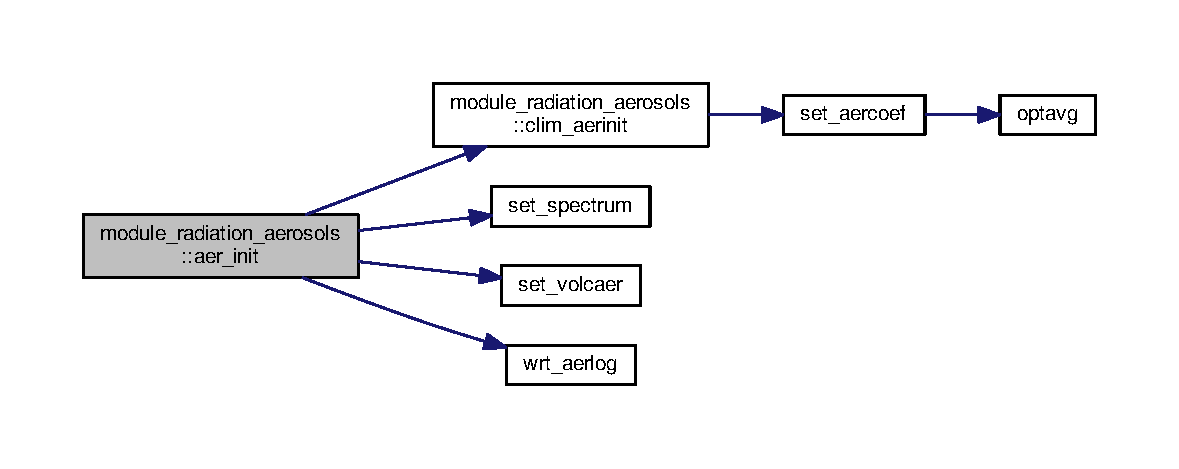
\includegraphics[width=350pt]{group__module__radiation__aerosols_ga58ac70a5189ef62c63cf2c87465a030a_cgraph}
\end{center}
\end{figure}
\mbox{\Hypertarget{group__module__radiation__aerosols_ga494892c147b1e14ffb241e413bc17a8b}\label{group__module__radiation__aerosols_ga494892c147b1e14ffb241e413bc17a8b}} 
\index{module\+\_\+radiation\+\_\+aerosols@{module\+\_\+radiation\+\_\+aerosols}!aer\+\_\+property@{aer\+\_\+property}}
\index{aer\+\_\+property@{aer\+\_\+property}!module\+\_\+radiation\+\_\+aerosols@{module\+\_\+radiation\+\_\+aerosols}}
\subsubsection{\texorpdfstring{aer\+\_\+property()}{aer\_property()}}
{\footnotesize\ttfamily subroutine module\+\_\+radiation\+\_\+aerosols\+::aer\+\_\+property (\begin{DoxyParamCaption}\item[{real (kind=kind\+\_\+phys), dimension(\+:,\+:), intent(in)}]{prsi,  }\item[{real (kind=kind\+\_\+phys), dimension(\+:,\+:), intent(in)}]{prsl,  }\item[{real (kind=kind\+\_\+phys), dimension(\+:,\+:), intent(in)}]{prslk,  }\item[{real (kind=kind\+\_\+phys), dimension(\+:,\+:), intent(in)}]{tvly,  }\item[{real (kind=kind\+\_\+phys), dimension(\+:,\+:), intent(in)}]{rhlay,  }\item[{real (kind=kind\+\_\+phys), dimension(\+:,\+:), intent(in)}]{dz,  }\item[{real (kind=kind\+\_\+phys), dimension(\+:,\+:), intent(in)}]{hz,  }\item[{real (kind=kind\+\_\+phys), dimension(\+:,\+:,\+:), intent(in)}]{tracer,  }\item[{real (kind=kind\+\_\+phys), dimension(\+:), intent(in)}]{alon,  }\item[{real (kind=kind\+\_\+phys), dimension(\+:), intent(in)}]{alat,  }\item[{real (kind=kind\+\_\+phys), dimension(\+:), intent(in)}]{slmsk,  }\item[{logical, intent(in)}]{laersw,  }\item[{logical, intent(in)}]{laerlw,  }\item[{integer, intent(in)}]{I\+M\+AX,  }\item[{integer, intent(in)}]{N\+L\+AY,  }\item[{integer, intent(in)}]{N\+L\+P1,  }\item[{real (kind=kind\+\_\+phys), dimension(\+:,\+:,\+:,\+:), intent(out)}]{aerosw,  }\item[{real (kind=kind\+\_\+phys), dimension(\+:,\+:,\+:,\+:), intent(out)}]{aerolw,  }\item[{real (kind=kind\+\_\+phys), dimension(\+:,\+:), intent(out)}]{aerodp }\end{DoxyParamCaption})\hspace{0.3cm}{\ttfamily [private]}}


\begin{DoxyParams}{Parameters}
{\em prsi} & (I\+M\+AX,N\+L\+P1), pressure at interface in mb \\
\hline
{\em prsl} & (I\+M\+AX,N\+L\+AY), layer mean pressure(not used) \\
\hline
{\em prslk} & (I\+M\+AX,N\+L\+AY), exner function= $(p/p0)^{rocp}$ (not used) \\
\hline
{\em tvly} & (I\+M\+AX,N\+L\+AY), layer virtual temperature (not used) \\
\hline
{\em rhlay} & (I\+M\+AX,N\+L\+AY), layer mean relative humidity \\
\hline
{\em dz} & (I\+M\+AX,N\+L\+AY), layer thickness in m \\
\hline
{\em hz} & (I\+M\+AX,N\+L\+P1), level high in m \\
\hline
{\em tracer} & (I\+M\+AX,N\+L\+AY,N\+T\+R\+AC), aer tracer concentrations (not used) \\
\hline
{\em alon,alat} & (I\+M\+AX), longitude and latitude of given points in degree \\
\hline
{\em slmsk} & (I\+M\+AX), sea/land mask (sea\+:0,land\+:1,sea-\/ice\+:2) \\
\hline
{\em laersw,laerlw} & logical flag for sw/lw aerosol calculations \\
\hline
{\em I\+M\+AX} & horizontal dimension of arrays \\
\hline
{\em N\+L\+AY,N\+L\+P1} & vertical dimensions of arrays \\
\hline
{\em N\+S\+PC} & num of species for optional aod output fields \\
\hline
{\em aerosw} & (I\+M\+AX,N\+L\+AY,N\+B\+D\+SW,N\+F\+\_\+\+A\+E\+SW), aeros opt properties for sw ~\newline
 (\+:,\+:,\+:,1)\+: optical depth ~\newline
 (\+:,\+:,\+:,2)\+: single scattering albedo ~\newline
 (\+:,\+:,\+:,3)\+: asymmetry parameter \\
\hline
{\em aerolw} & (I\+M\+AX,N\+L\+AY,N\+B\+D\+LW,N\+F\+\_\+\+A\+E\+LW), aeros opt properties for lw ~\newline
 (\+:,\+:,\+:,1)\+: optical depth ~\newline
 (\+:,\+:,\+:,2)\+: single scattering albedo ~\newline
 (\+:,\+:,\+:,3)\+: asymmetry parameter \\
\hline
{\em aerodp} & (I\+M\+AX,N\+S\+P\+C+1), vertically integrated aer-\/opt-\/depth \\
\hline
\end{DoxyParams}
\hypertarget{group__module__radiation__aerosols_gel_aer_pro}{}\subsection{General Algorithm}\label{group__module__radiation__aerosols_gel_aer_pro}

\begin{DoxyEnumerate}
\item Map aerosol data to model grids
\begin{DoxyItemize}
\item Map grid in longitude direction, lon from 0 to 355 deg resolution
\item Map grid in latitude direction, lat from 90n to 90s in 5 deg resolution
\end{DoxyItemize}
\item Determin the type of aerosol profile (kp) and scale hight for domain 1 (h1) to be used at this grid point.
\item Compute horizontal bi-\/linear interpolation weights
\item Do horizontal bi-\/linear interpolation on aerosol partical density (denn)
\item Do horizontal bi-\/linear interpolation on mixing ratios
\item Prepare to setup domain index array and effective layer thickness, also convert pressure level to sigma level to follow the terrain.
\item Call \hyperlink{group__module__radiation__aerosols_gae60b55ebc37825b2c3c95f95b23ed558}{radclimaer()} to calculate S\+W/\+LW aerosol optical properties for the corresponding frequency bands. 
\end{DoxyEnumerate}

Definition at line 2774 of file radiation\+\_\+aerosols.\+f.



References cmixg, denng, haer, idxcg, imxae, jmxae, kprfg, nlwbnd, nspc, nswbnd, nv\+\_\+aod, nxc, prsref, radclimaer(), and sigref.



Referenced by setaer().

Here is the call graph for this function\+:
% FIG 0
\mbox{\Hypertarget{group__module__radiation__aerosols_ga237071d2a0691d5aae199937d9b6aca5}\label{group__module__radiation__aerosols_ga237071d2a0691d5aae199937d9b6aca5}} 
\index{module\+\_\+radiation\+\_\+aerosols@{module\+\_\+radiation\+\_\+aerosols}!aer\+\_\+update@{aer\+\_\+update}}
\index{aer\+\_\+update@{aer\+\_\+update}!module\+\_\+radiation\+\_\+aerosols@{module\+\_\+radiation\+\_\+aerosols}}
\subsubsection{\texorpdfstring{aer\+\_\+update()}{aer\_update()}}
{\footnotesize\ttfamily subroutine, public module\+\_\+radiation\+\_\+aerosols\+::aer\+\_\+update (\begin{DoxyParamCaption}\item[{integer, intent(in)}]{iyear,  }\item[{integer, intent(in)}]{imon,  }\item[{integer, intent(in)}]{me }\end{DoxyParamCaption})}


\begin{DoxyParams}{Parameters}
{\em iyear} & 4-\/digit calender year \\
\hline
{\em imon} & month of the year \\
\hline
{\em me} & print message control flag \\
\hline
\end{DoxyParams}
\hypertarget{group__module__radiation__aerosols_gen_aer_upd}{}\subsection{General Algorithm}\label{group__module__radiation__aerosols_gen_aer_upd}

\begin{DoxyEnumerate}
\item Call \hyperlink{group__module__radiation__aerosols_gafac9a9c603c033c8511e8dbfe984f703}{trop\+\_\+update()} to update monthly tropospheric aerosol data.
\item Call \hyperlink{group__module__radiation__aerosols_ga6ec9bd68d45a5f2c6bb9997bdad420c3}{volc\+\_\+update()} to update yearly stratospheric volcanic aerosol data. 
\end{DoxyEnumerate}

Definition at line 1806 of file radiation\+\_\+aerosols.\+f.



References trop\+\_\+update(), and volc\+\_\+update().



Referenced by module\+\_\+radiation\+\_\+driver\+::radupdate().

Here is the call graph for this function\+:\nopagebreak
\begin{figure}[H]
\begin{center}
\leavevmode
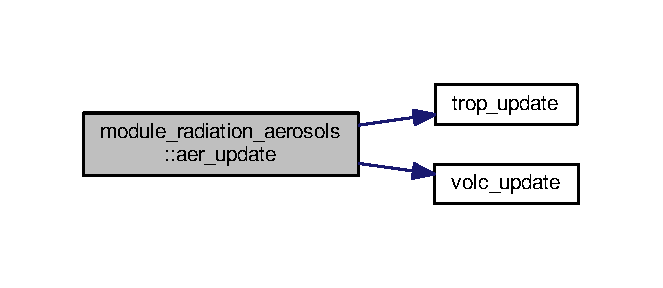
\includegraphics[width=318pt]{group__module__radiation__aerosols_ga237071d2a0691d5aae199937d9b6aca5_cgraph}
\end{center}
\end{figure}
\mbox{\Hypertarget{group__module__radiation__aerosols_gacdc24d7d4c01b97920ef940cc01c9cc0}\label{group__module__radiation__aerosols_gacdc24d7d4c01b97920ef940cc01c9cc0}} 
\index{module\+\_\+radiation\+\_\+aerosols@{module\+\_\+radiation\+\_\+aerosols}!clim\+\_\+aerinit@{clim\+\_\+aerinit}}
\index{clim\+\_\+aerinit@{clim\+\_\+aerinit}!module\+\_\+radiation\+\_\+aerosols@{module\+\_\+radiation\+\_\+aerosols}}
\subsubsection{\texorpdfstring{clim\+\_\+aerinit()}{clim\_aerinit()}}
{\footnotesize\ttfamily subroutine module\+\_\+radiation\+\_\+aerosols\+::clim\+\_\+aerinit (\begin{DoxyParamCaption}\item[{real (kind=kind\+\_\+phys), dimension(\+:)}]{solfwv,  }\item[{real (kind=kind\+\_\+phys), dimension(\+:)}]{eirfwv,  }\item[{integer, intent(in)}]{me }\end{DoxyParamCaption})\hspace{0.3cm}{\ttfamily [private]}}


\begin{DoxyParams}{Parameters}
{\em solfwv} & (N\+W\+V\+T\+OT), solar flux for each individual wavenumber $(w/m^2)$ \\
\hline
{\em eirfwv} & (N\+W\+V\+T\+IR), IR flux(273k) for each individual wavenumber $(w/m^2)$ \\
\hline
{\em me} & print message control flag\\
\hline
\end{DoxyParams}
\hypertarget{group__module__radiation__aerosols_gen_clim_aerinit}{}\subsection{General Algorithm}\label{group__module__radiation__aerosols_gen_clim_aerinit}

\begin{DoxyItemize}
\item call \hyperlink{group__module__radiation__aerosols_ga95fabbc4272ae70f3b345f9b1a898d46}{set\+\_\+aercoef()} to invoke tropospheric aerosol initialization. 
\end{DoxyItemize}

Definition at line 1083 of file radiation\+\_\+aerosols.\+f.



References set\+\_\+aercoef().



Referenced by aer\+\_\+init().

Here is the call graph for this function\+:
% FIG 1
\mbox{\Hypertarget{group__module__radiation__aerosols_ga579538840d4d8c86efa155b788c14ae3}\label{group__module__radiation__aerosols_ga579538840d4d8c86efa155b788c14ae3}} 
\index{module\+\_\+radiation\+\_\+aerosols@{module\+\_\+radiation\+\_\+aerosols}!gocart\+\_\+init@{gocart\+\_\+init}}
\index{gocart\+\_\+init@{gocart\+\_\+init}!module\+\_\+radiation\+\_\+aerosols@{module\+\_\+radiation\+\_\+aerosols}}
\subsubsection{\texorpdfstring{gocart\+\_\+init()}{gocart\_init()}}
{\footnotesize\ttfamily subroutine module\+\_\+radiation\+\_\+aerosols\+::gocart\+\_\+init (\begin{DoxyParamCaption}\item[{integer, intent(in)}]{N\+W\+V\+T\+OT,  }\item[{real (kind=kind\+\_\+phys), dimension(\+:), intent(in)}]{solfwv,  }\item[{real (kind=kind\+\_\+phys), intent(in)}]{soltot,  }\item[{integer, intent(in)}]{N\+W\+V\+T\+IR,  }\item[{real (kind=kind\+\_\+phys), dimension(\+:), intent(in)}]{eirfwv,  }\item[{integer, intent(in)}]{N\+B\+D\+SW,  }\item[{integer, intent(in)}]{N\+L\+W\+B\+ND,  }\item[{integer, intent(in)}]{N\+S\+W\+L\+W\+BD,  }\item[{integer, intent(in)}]{imon,  }\item[{integer, intent(in)}]{me,  }\item[{real (kind=kind\+\_\+phys), intent(in)}]{raddt,  }\item[{real (kind=kind\+\_\+phys), intent(in)}]{fdaer }\end{DoxyParamCaption})\hspace{0.3cm}{\ttfamily [private]}}


\begin{DoxyItemize}
\item determine weight and index for aerosol composition/luts
\item read in monthly global distribution of gocart aerosols
\item read and map the tabulated aerosol optical spectral data onto corresponding S\+W/\+LW radiation spectral bands.
\end{DoxyItemize}


\begin{DoxyParams}{Parameters}
{\em N\+W\+V\+T\+OT} & total num of wave numbers used in sw spectrum \\
\hline
{\em solfwv} & (N\+W\+V\+T\+OT), solar flux for each individual wavenumber (w/m2) \\
\hline
{\em soltot} & total solar flux for the spectrual range (w/m2) \\
\hline
{\em N\+W\+V\+T\+IR} & total num of wave numbers used in the ir region \\
\hline
{\em eirfwv} & (N\+W\+V\+T\+IR), ir flux(273k) for each individual wavenumber (w/m2) \\
\hline
{\em N\+B\+D\+SW} & num of bands calculated for sw aeros opt prop \\
\hline
{\em N\+L\+W\+B\+ND} & num of bands calculated for lw aeros opt prop \\
\hline
{\em N\+S\+W\+L\+W\+BD} & total num of bands calc for sw+lw aeros opt prop \\
\hline
{\em imon} & month of the year \\
\hline
{\em me} & print message control flag \\
\hline
{\em raddt} & \\
\hline
{\em fdaer} & \\
\hline
\end{DoxyParams}
\hypertarget{group__module__radiation__aerosols_gel_go_ini}{}\subsection{General Algorithm}\label{group__module__radiation__aerosols_gel_go_ini}


Definition at line 3533 of file radiation\+\_\+aerosols.\+f.



References extrhd\+\_\+grt, extrhi\+\_\+grt, get\+\_\+clim, iendwv\+\_\+grt, kaerbnd, krhlev, lckprnt, lgrtint, module\+\_\+radsw\+\_\+parameters\+::nswstr, nv\+\_\+aod, optavg\+\_\+grt(), rd\+\_\+gocart\+\_\+clim(), rd\+\_\+gocart\+\_\+luts(), rhdpasy0\+\_\+grt, rhdpext0\+\_\+grt, rhdpssa0\+\_\+grt, rhidasy0\+\_\+grt, rhidext0\+\_\+grt, rhidssa0\+\_\+grt, and set\+\_\+aerspc().

Here is the call graph for this function\+:
% FIG 2
\mbox{\Hypertarget{group__module__radiation__aerosols_ga15bad8499ffd17d967e5788cd6721c4d}\label{group__module__radiation__aerosols_ga15bad8499ffd17d967e5788cd6721c4d}} 
\index{module\+\_\+radiation\+\_\+aerosols@{module\+\_\+radiation\+\_\+aerosols}!rd\+\_\+gocart\+\_\+clim@{rd\+\_\+gocart\+\_\+clim}}
\index{rd\+\_\+gocart\+\_\+clim@{rd\+\_\+gocart\+\_\+clim}!module\+\_\+radiation\+\_\+aerosols@{module\+\_\+radiation\+\_\+aerosols}}
\subsubsection{\texorpdfstring{rd\+\_\+gocart\+\_\+clim()}{rd\_gocart\_clim()}}
{\footnotesize\ttfamily subroutine gocart\+\_\+init\+::rd\+\_\+gocart\+\_\+clim (\begin{DoxyParamCaption}{ }\end{DoxyParamCaption})\hspace{0.3cm}{\ttfamily [private]}}


\begin{DoxyItemize}
\item 1. read in aerosol dry mass and surface pressure from G\+E\+O\+S3-\/\+G\+O\+C\+A\+RT C3.\+1 2000 monthly dataset or aerosol mixing ratio and surface pressure from G\+E\+O\+S4-\/\+G\+O\+C\+A\+RT 2000-\/2007 averaged monthly data set.
\item 2. compute goes lat/lon array (for horizontal mapping) 
\end{DoxyItemize}

Definition at line 4543 of file radiation\+\_\+aerosols.\+f.



References dmclmg, geos\+\_\+rlat, geos\+\_\+rlon, gocart\+\_\+climo, gridcomp, imxg, jmxg, kmxg, molwgt, nmxg, nswlwbd, num\+\_\+gridcomp, and psclmg.



Referenced by gocart\+\_\+init().

\mbox{\Hypertarget{group__module__radiation__aerosols_ga95fabbc4272ae70f3b345f9b1a898d46}\label{group__module__radiation__aerosols_ga95fabbc4272ae70f3b345f9b1a898d46}} 
\index{module\+\_\+radiation\+\_\+aerosols@{module\+\_\+radiation\+\_\+aerosols}!set\+\_\+aercoef@{set\+\_\+aercoef}}
\index{set\+\_\+aercoef@{set\+\_\+aercoef}!module\+\_\+radiation\+\_\+aerosols@{module\+\_\+radiation\+\_\+aerosols}}
\subsubsection{\texorpdfstring{set\+\_\+aercoef()}{set\_aercoef()}}
{\footnotesize\ttfamily subroutine clim\+\_\+aerinit\+::set\+\_\+aercoef (\begin{DoxyParamCaption}{ }\end{DoxyParamCaption})\hspace{0.3cm}{\ttfamily [private]}}

\hypertarget{group__module__radiation__aerosols_det_set_aercoef}{}\subsection{General Algorithm}\label{group__module__radiation__aerosols_det_set_aercoef}

\begin{DoxyEnumerate}
\item Reading climatological aerosols optical data from aeros\+\_\+file, including\+:
\begin{DoxyItemize}
\item ending wave num for 61 aerosol spectral bands
\item atmos scale height for 5 domains, 7 profs
\item reference pressure for 5 domains, 7 profs
\item rh independent ext coef for 61 bands, 6 species
\item rh independent sca coef for 61 bands, 6 species
\item rh independent ssa coef for 61 bands, 6 species
\item rh independent asy coef for 61 bands, 6 species
\item rh dependent ext coef for 61 bands, 8 rh lev, 4 species
\item rh dependent sca coef for 61 bands, 8 rh lev, 4 species
\item rh dependent ssa coef for 61 bands, 8 rh lev, 4 species
\item rh dependent asy coef for 61 bands, 8 rh lev, 4 species
\item stratospheric background aeros for 61 bands
\end{DoxyItemize}
\item Convert pressure reference level (in mb) to sigma reference level assume an 1000mb reference surface pressure.
\item Compute solar flux weights and interval indices for mapping spectral bands between SW radiation and aerosol data.
\item Compute LW flux weights and interval indices for mapping spectral bands between lw radiation and aerosol data.
\item Call \hyperlink{group__module__radiation__aerosols_ga637761b6110739f2d96322e2ddcc1291}{optavg()} to compute spectral band mean properties for each species. 
\end{DoxyEnumerate}

Definition at line 1172 of file radiation\+\_\+aerosols.\+f.



References haer, imxae, jmxae, naerbnd, ncm1, ncm2, nlwbnd, nlwstr, nrhlev, nswbnd, nswlwbd, module\+\_\+radsw\+\_\+parameters\+::nswstr, nv\+\_\+aod, optavg(), prsref, sigref, and wvn550.



Referenced by clim\+\_\+aerinit().

Here is the call graph for this function\+:\nopagebreak
\begin{figure}[H]
\begin{center}
\leavevmode
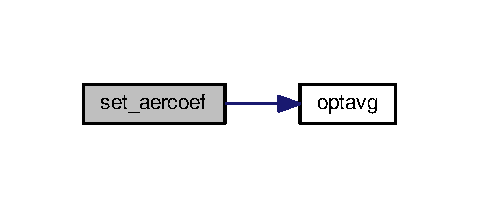
\includegraphics[width=230pt]{group__module__radiation__aerosols_ga95fabbc4272ae70f3b345f9b1a898d46_cgraph}
\end{center}
\end{figure}
\mbox{\Hypertarget{group__module__radiation__aerosols_gaa7fe6dc2964bc474a132b93aaab82cb0}\label{group__module__radiation__aerosols_gaa7fe6dc2964bc474a132b93aaab82cb0}} 
\index{module\+\_\+radiation\+\_\+aerosols@{module\+\_\+radiation\+\_\+aerosols}!set\+\_\+spectrum@{set\+\_\+spectrum}}
\index{set\+\_\+spectrum@{set\+\_\+spectrum}!module\+\_\+radiation\+\_\+aerosols@{module\+\_\+radiation\+\_\+aerosols}}
\subsubsection{\texorpdfstring{set\+\_\+spectrum()}{set\_spectrum()}}
{\footnotesize\ttfamily subroutine aer\+\_\+init\+::set\+\_\+spectrum (\begin{DoxyParamCaption}{ }\end{DoxyParamCaption})\hspace{0.3cm}{\ttfamily [private]}}


\begin{DoxyItemize}
\item inputs\+: (module constants)
\begin{DoxyItemize}
\item N\+W\+V\+T\+OT\+: total num of wave numbers used in sw spectrum
\item N\+W\+V\+T\+IR\+: total num of wave numbers used in the ir region
\end{DoxyItemize}
\item outputs\+: (in-\/scope variables)
\begin{DoxyItemize}
\item solfwv(\+N\+W\+V\+T\+O\+T)\+: solar flux for each individual wavenumber ( $W/m^2$)
\item eirfwv(\+N\+W\+V\+T\+I\+R)\+: ir flux(273k) for each individual wavenumber ( $W/m^2$) 
\end{DoxyItemize}
\end{DoxyItemize}

Definition at line 933 of file radiation\+\_\+aerosols.\+f.



References nwvns0, nwvsol, nwvtir, and s0intv.



Referenced by aer\+\_\+init().

\mbox{\Hypertarget{group__module__radiation__aerosols_ga184fcc0618c1c4d42fa08cfe1e20e5c1}\label{group__module__radiation__aerosols_ga184fcc0618c1c4d42fa08cfe1e20e5c1}} 
\index{module\+\_\+radiation\+\_\+aerosols@{module\+\_\+radiation\+\_\+aerosols}!setaer@{setaer}}
\index{setaer@{setaer}!module\+\_\+radiation\+\_\+aerosols@{module\+\_\+radiation\+\_\+aerosols}}
\subsubsection{\texorpdfstring{setaer()}{setaer()}}
{\footnotesize\ttfamily subroutine, public module\+\_\+radiation\+\_\+aerosols\+::setaer (\begin{DoxyParamCaption}\item[{real (kind=kind\+\_\+phys), dimension(\+:,\+:), intent(in)}]{prsi,  }\item[{real (kind=kind\+\_\+phys), dimension(\+:,\+:), intent(in)}]{prsl,  }\item[{real (kind=kind\+\_\+phys), dimension(\+:,\+:), intent(in)}]{prslk,  }\item[{real (kind=kind\+\_\+phys), dimension(\+:,\+:), intent(in)}]{tvly,  }\item[{real (kind=kind\+\_\+phys), dimension(\+:,\+:), intent(in)}]{rhlay,  }\item[{real (kind=kind\+\_\+phys), dimension(\+:), intent(in)}]{slmsk,  }\item[{real (kind=kind\+\_\+phys), dimension(\+:,\+:,\+:), intent(in)}]{tracer,  }\item[{real (kind=kind\+\_\+phys), dimension(\+:), intent(in)}]{xlon,  }\item[{real (kind=kind\+\_\+phys), dimension(\+:), intent(in)}]{xlat,  }\item[{integer, intent(in)}]{I\+M\+AX,  }\item[{integer, intent(in)}]{N\+L\+AY,  }\item[{integer, intent(in)}]{N\+L\+P1,  }\item[{logical, intent(in)}]{lsswr,  }\item[{logical, intent(in)}]{lslwr,  }\item[{real (kind=kind\+\_\+phys), dimension(\+:,\+:,\+:,\+:), intent(out)}]{aerosw,  }\item[{real (kind=kind\+\_\+phys), dimension(\+:,\+:,\+:,\+:), intent(out)}]{aerolw,  }\item[{real (kind=kind\+\_\+phys), dimension(\+:,\+:), intent(out)}]{aerodp }\end{DoxyParamCaption})}


\begin{DoxyParams}{Parameters}
{\em prsi} & (I\+M\+AX,N\+L\+P1), pressure at interface in mb \\
\hline
{\em prsl} & (I\+M\+AX,N\+L\+AY), layer mean pressure in mb \\
\hline
{\em prslk} & (I\+M\+AX,N\+L\+AY), exner function = $(p/p0)^{rocp}$ \\
\hline
{\em tvly} & (I\+M\+AX,N\+L\+AY), layer virtual temperature in K \\
\hline
{\em rhlay} & (I\+M\+AX,N\+L\+AY), layer mean relative humidity \\
\hline
{\em slmsk} & (I\+M\+AX), sea/land mask (sea\+:0,land\+:1,sea-\/ice\+:2) \\
\hline
{\em tracer} & (I\+M\+AX,N\+L\+AY,N\+T\+R\+AC), aerosol tracer concentration \\
\hline
{\em xlon} & (I\+M\+AX), longitude of given points in radiance, ok for both 0-\/$>$2pi or -\/pi-\/$>$+pi ranges \\
\hline
{\em xlat} & (I\+M\+AX), latitude of given points in radiance, default to pi/2 -\/$>$ -\/pi/2, otherwise see in-\/line comment \\
\hline
{\em I\+M\+AX} & 1, horizontal dimension of arrays \\
\hline
{\em N\+L\+AY,N\+L\+P1} & 1, vertical dimensions of arrays \\
\hline
{\em lsswr,lslwr} & logical flags for sw/lw radiation calls \\
\hline
{\em aerosw} & (I\+M\+AX,N\+L\+AY,N\+B\+D\+SW,N\+F\+\_\+\+A\+E\+SW), aeros opt properties for sw ~\newline
 (\+:,\+:,\+:,1)\+: optical depth ~\newline
 (\+:,\+:,\+:,2)\+: single scattering albedo ~\newline
 (\+:,\+:,\+:,3)\+: asymmetry parameter \\
\hline
{\em aerolw} & (I\+M\+AX,N\+L\+AY,N\+B\+D\+LW,N\+F\+\_\+\+A\+E\+LW), aeros opt properties for lw ~\newline
 (\+:,\+:,\+:,1)\+: optical depth ~\newline
 (\+:,\+:,\+:,2)\+: single scattering albedo ~\newline
 (\+:,\+:,\+:,3)\+: asymmetry parameter \\
\hline
{\em aerodp} & (I\+M\+AX,N\+S\+P\+C1), vertically integrated optical depth \\
\hline
\end{DoxyParams}
\hypertarget{group__module__radiation__aerosols_general_setaer}{}\subsection{General Algorithm}\label{group__module__radiation__aerosols_general_setaer}

\begin{DoxyEnumerate}
\item Convert lat/lon from radiance to degree.
\item Compute level height and layer thickness.
\item Calculate SW aerosol optical properties for the corresponding frequency bands\+:
\begin{DoxyItemize}
\item if opac aerosol climatology is used, call \hyperlink{group__module__radiation__aerosols_ga494892c147b1e14ffb241e413bc17a8b}{aer\+\_\+property()}\+: this subroutine maps the 5 degree global climatological aerosol data set onto model grids, and compute aerosol optical properties for SW and LW radiations.
\item if gocart aerosol scheme is used, call \hyperlink{group__module__radiation__aerosols_ga04ce3c11b81d0a0b025f79c4f29acfb8}{setgocartaer()}\+: this subroutine computes sw + lw aerosol optical properties for gocart aerosol species (merged from fcst and clim fields).
\end{DoxyItemize}
\item Compute stratosphere volcanic forcing\+:
\begin{DoxyItemize}
\item select data in 4 lat bands, interpolation at the boundaries
\item Find lower boundary of stratosphere\+: polar, fixed at 25000pa (250mb); tropic, fixed at 15000pa (150mb); mid-\/lat, interpolation
\item SW\+: add volcanic aerosol optical depth to the background value
\item Smoothing profile at boundary if needed
\item LW\+: add volcanic aerosol optical depth to the background value 
\end{DoxyItemize}
\end{DoxyEnumerate}

Definition at line 2186 of file radiation\+\_\+aerosols.\+f.



References aer\+\_\+property(), ivolae, kmonsav, kyrsav, nf\+\_\+aelw, nf\+\_\+aesw, nlwbnd, nspc1, nswlwbd, module\+\_\+radsw\+\_\+parameters\+::nswstr, and setgocartaer().



Referenced by module\+\_\+radiation\+\_\+driver\+::gfs\+\_\+radiation\+\_\+driver().

Here is the call graph for this function\+:
% FIG 3
\mbox{\Hypertarget{group__module__radiation__aerosols_ga04ce3c11b81d0a0b025f79c4f29acfb8}\label{group__module__radiation__aerosols_ga04ce3c11b81d0a0b025f79c4f29acfb8}} 
\index{module\+\_\+radiation\+\_\+aerosols@{module\+\_\+radiation\+\_\+aerosols}!setgocartaer@{setgocartaer}}
\index{setgocartaer@{setgocartaer}!module\+\_\+radiation\+\_\+aerosols@{module\+\_\+radiation\+\_\+aerosols}}
\subsubsection{\texorpdfstring{setgocartaer()}{setgocartaer()}}
{\footnotesize\ttfamily subroutine module\+\_\+radiation\+\_\+aerosols\+::setgocartaer (\begin{DoxyParamCaption}\item[{real (kind=kind\+\_\+phys), dimension(\+:), intent(in)}]{alon,  }\item[{real (kind=kind\+\_\+phys), dimension(\+:), intent(in)}]{alat,  }\item[{real (kind=kind\+\_\+phys), dimension(\+:,\+:), intent(in)}]{prslk,  }\item[{real (kind=kind\+\_\+phys), dimension(\+:,\+:), intent(in)}]{rhlay,  }\item[{real (kind=kind\+\_\+phys), dimension(\+:,\+:), intent(in)}]{dz,  }\item[{real (kind=kind\+\_\+phys), dimension(\+:,\+:), intent(in)}]{hz,  }\item[{integer, intent(in)}]{N\+S\+W\+L\+W\+BD,  }\item[{real (kind=kind\+\_\+phys), dimension(\+:,\+:), intent(in)}]{prsl,  }\item[{real (kind=kind\+\_\+phys), dimension(\+:,\+:), intent(in)}]{tvly,  }\item[{real (kind=kind\+\_\+phys), dimension(\+:,\+:,\+:), intent(in)}]{trcly,  }\item[{integer, intent(in)}]{I\+M\+AX,  }\item[{integer, intent(in)}]{N\+L\+AY,  }\item[{integer, intent(in)}]{N\+L\+P1,  }\item[{integer, intent(in)}]{ivflip,  }\item[{logical, intent(in)}]{lsswr,  }\item[{logical, intent(in)}]{lslwr,  }\item[{real (kind=kind\+\_\+phys), dimension(\+:,\+:,\+:,\+:), intent(out)}]{aerosw,  }\item[{real (kind=kind\+\_\+phys), dimension(\+:,\+:,\+:,\+:), intent(out)}]{aerolw }\end{DoxyParamCaption})\hspace{0.3cm}{\ttfamily [private]}}


\begin{DoxyParams}{Parameters}
{\em alon} & I\+M\+AX, longitude of given points in degree \\
\hline
{\em alat} & I\+M\+AX, latitude of given points in degree \\
\hline
{\em prslk} & (I\+M\+AX,N\+L\+AY), pressure in cb \\
\hline
{\em rhlay} & (I\+M\+AX,N\+L\+AY), layer mean relative humidity \\
\hline
{\em dz} & (I\+M\+AX,N\+L\+AY), layer thickness in m \\
\hline
{\em hz} & (I\+M\+AX,N\+L\+P1), level high in m \\
\hline
{\em N\+S\+W\+L\+W\+BD} & total number of sw+ir bands for aeros opt prop \\
\hline
{\em prsl} & (I\+M\+AX,N\+L\+AY), layer mean pressure in mb \\
\hline
{\em tvly} & (I\+M\+AX,N\+L\+AY), layer mean virtual temperature in K \\
\hline
{\em trcly} & (I\+M\+AX,N\+L\+AY,N\+T\+R\+AC), layer mean specific tracer in g/g \\
\hline
{\em I\+M\+AX} & horizontal dimension of arrays \\
\hline
{\em N\+L\+AY,N\+L\+P1} & vertical dimensions of arrays \\
\hline
{\em ivflip} & control flag for direction of vertical index ~\newline
 =0\+: index from toa to surface ~\newline
 =1\+: index from surface to toa \\
\hline
{\em lsswr,lslwr} & logical flag for sw/lw radiation calls \\
\hline
{\em aerosw} & (I\+M\+AX,N\+L\+AY,N\+B\+D\+SW,N\+F\+\_\+\+A\+E\+SW), aeros opt properties for SW ~\newline
 (\+:,\+:,\+:,1)\+: optical depth ~\newline
 (\+:,\+:,\+:,2)\+: single scattering albedo ~\newline
 (\+:,\+:,\+:,3)\+: asymmetry parameter \\
\hline
{\em aerolw} & (I\+M\+AX,N\+L\+AY,N\+B\+D\+LW,N\+F\+\_\+\+A\+E\+LW), aeros opt properties for LW ~\newline
 (\+:,\+:,\+:,1)\+: optical depth ~\newline
 (\+:,\+:,\+:,2)\+: single scattering albedo ~\newline
 (\+:,\+:,\+:,3)\+: asymmetry parameter \\
\hline
\end{DoxyParams}
\hypertarget{group__module__radiation__aerosols_gen_setgo}{}\subsection{General Algorithm}\label{group__module__radiation__aerosols_gen_setgo}

\begin{DoxyEnumerate}
\item Call \hyperlink{group__module__radiation__aerosols_ga651c4be2fa354238990c5c7b9488e9fd}{map\+\_\+aermr()} to map input tracer array (trcly) to local tracer array (aermr).
\item Map geos-\/gocart climo (dmclmg) to gfs grids (dmclm).
\item Call \hyperlink{group__module__radiation__aerosols_ga4ff866c545425e7029a11999e97d8faa}{aeropt\+\_\+grt()} to alculate sw/lw aerosol optical properties for the corresponding frequency bands. 
\end{DoxyEnumerate}

Definition at line 4898 of file radiation\+\_\+aerosols.\+f.



References aeropt\+\_\+grt(), ctaer, dmclmg, geos\+\_\+rlat, geos\+\_\+rlon, get\+\_\+clim, get\+\_\+fcst, gocart\+\_\+climo, imxg, jmxg, kmxg, map\+\_\+aermr(), molwgt, nlwbnd, nmxg, and psclmg.



Referenced by setaer().

Here is the call graph for this function\+:
% FIG 4

\hypertarget{group__module__radiation__astronomy}{}\section{module\+\_\+radiation\+\_\+astronomy}
\label{group__module__radiation__astronomy}\index{module\+\_\+radiation\+\_\+astronomy@{module\+\_\+radiation\+\_\+astronomy}}


This module sets up astronomical quantities for solar radiation calculations.  




\subsection{Detailed Description}
\begin{DoxyVersion}{Version}
N\+C\+E\+P-\/\+Radiation\+\_\+astronomy v5.\+2 Jan 2013 
\end{DoxyVersion}
\subsection*{Parameter constants}
\begin{DoxyCompactItemize}
\item 
\mbox{\Hypertarget{group__module__radiation__astronomy_ga220d2b997b3073cf2985d62111c5405d}\label{group__module__radiation__astronomy_ga220d2b997b3073cf2985d62111c5405d}} 
real(kind=kind\+\_\+phys), parameter {\bfseries module\+\_\+radiation\+\_\+astronomy\+::degrad} = 180.\+0/con\+\_\+pi
\item 
\mbox{\Hypertarget{group__module__radiation__astronomy_ga4fbf4be04e17f1f8d0674ee2e20506b0}\label{group__module__radiation__astronomy_ga4fbf4be04e17f1f8d0674ee2e20506b0}} 
real(kind=kind\+\_\+phys), parameter {\bfseries module\+\_\+radiation\+\_\+astronomy\+::tpi} = 2.\+0 $\ast$ con\+\_\+pi
\item 
\mbox{\Hypertarget{group__module__radiation__astronomy_ga7369d8561566f5e7e51ccc40e09f2520}\label{group__module__radiation__astronomy_ga7369d8561566f5e7e51ccc40e09f2520}} 
real(kind=kind\+\_\+phys), parameter {\bfseries module\+\_\+radiation\+\_\+astronomy\+::hpi} = 0.\+5 $\ast$ con\+\_\+pi
\item 
\mbox{\Hypertarget{group__module__radiation__astronomy_gad59856e8f877eb05a6b22610f14a391d}\label{group__module__radiation__astronomy_gad59856e8f877eb05a6b22610f14a391d}} 
real(kind=kind\+\_\+phys), parameter {\bfseries module\+\_\+radiation\+\_\+astronomy\+::f12} = 12.\+0
\item 
\mbox{\Hypertarget{group__module__radiation__astronomy_ga37b491dde50d06e339effb4a31d9f245}\label{group__module__radiation__astronomy_ga37b491dde50d06e339effb4a31d9f245}} 
real(kind=kind\+\_\+phys), parameter {\bfseries module\+\_\+radiation\+\_\+astronomy\+::f3600} = 3600.\+0
\item 
\mbox{\Hypertarget{group__module__radiation__astronomy_gafeb2fccbe8137de6099a09035762ff5e}\label{group__module__radiation__astronomy_gafeb2fccbe8137de6099a09035762ff5e}} 
real(kind=kind\+\_\+phys), parameter {\bfseries module\+\_\+radiation\+\_\+astronomy\+::czlimt} = 0.\+0001
\item 
\mbox{\Hypertarget{group__module__radiation__astronomy_gadbf9cdfc7b55d882f015a4bc4ef276ab}\label{group__module__radiation__astronomy_gadbf9cdfc7b55d882f015a4bc4ef276ab}} 
real(kind=kind\+\_\+phys), parameter {\bfseries module\+\_\+radiation\+\_\+astronomy\+::pid12} = (2.\+0$\ast$asin(1.\+0))/f12
\end{DoxyCompactItemize}
\subsection*{Module variable (to be set in module\+\_\+radiation\+\_\+astronomy\+:\+:sol\+\_\+init)\+:}
\begin{DoxyCompactItemize}
\item 
\mbox{\Hypertarget{group__module__radiation__astronomy_ga37e08872f67023b11f839ac15151af09}\label{group__module__radiation__astronomy_ga37e08872f67023b11f839ac15151af09}} 
real(kind=kind\+\_\+phys), public {\bfseries module\+\_\+radiation\+\_\+astronomy\+::solc0} = con\+\_\+solr
\item 
\mbox{\Hypertarget{group__module__radiation__astronomy_ga7ea431b6d4f4d6ee1f6545d6baeee44f}\label{group__module__radiation__astronomy_ga7ea431b6d4f4d6ee1f6545d6baeee44f}} 
integer {\bfseries module\+\_\+radiation\+\_\+astronomy\+::isolflg} = 10
\item 
\mbox{\Hypertarget{group__module__radiation__astronomy_ga05ee7e378d38b90242738b9bf6c40c00}\label{group__module__radiation__astronomy_ga05ee7e378d38b90242738b9bf6c40c00}} 
character(26) {\bfseries module\+\_\+radiation\+\_\+astronomy\+::solar\+\_\+fname} = \textquotesingle{} \textquotesingle{}
\end{DoxyCompactItemize}
\subsection*{Module variables (to be set in module\+\_\+radiation\+\_\+astronomy\+:\+:sol\+\_\+update)}
\begin{DoxyCompactItemize}
\item 
\mbox{\Hypertarget{group__module__radiation__astronomy_ga264a011aa71fb670339ac555dc24e486}\label{group__module__radiation__astronomy_ga264a011aa71fb670339ac555dc24e486}} 
real(kind=kind\+\_\+phys) \hyperlink{group__module__radiation__astronomy_ga264a011aa71fb670339ac555dc24e486}{module\+\_\+radiation\+\_\+astronomy\+::sollag} =0.\+0
\begin{DoxyCompactList}\small\item\em equation of time \end{DoxyCompactList}\item 
\mbox{\Hypertarget{group__module__radiation__astronomy_gae195d9c834e2789170f89c988d28b01e}\label{group__module__radiation__astronomy_gae195d9c834e2789170f89c988d28b01e}} 
real(kind=kind\+\_\+phys) \hyperlink{group__module__radiation__astronomy_gae195d9c834e2789170f89c988d28b01e}{module\+\_\+radiation\+\_\+astronomy\+::sindec} =0.\+0
\begin{DoxyCompactList}\small\item\em sine of the solar declination angle \end{DoxyCompactList}\item 
\mbox{\Hypertarget{group__module__radiation__astronomy_ga07386e90045639b8023abd826e0e2768}\label{group__module__radiation__astronomy_ga07386e90045639b8023abd826e0e2768}} 
real(kind=kind\+\_\+phys) \hyperlink{group__module__radiation__astronomy_ga07386e90045639b8023abd826e0e2768}{module\+\_\+radiation\+\_\+astronomy\+::cosdec} =0.\+0
\begin{DoxyCompactList}\small\item\em cosine of the solar declination angle \end{DoxyCompactList}\item 
\mbox{\Hypertarget{group__module__radiation__astronomy_ga723159a44491e4ae974128123a1e8dcd}\label{group__module__radiation__astronomy_ga723159a44491e4ae974128123a1e8dcd}} 
real(kind=kind\+\_\+phys) \hyperlink{group__module__radiation__astronomy_ga723159a44491e4ae974128123a1e8dcd}{module\+\_\+radiation\+\_\+astronomy\+::anginc} =0.\+0
\begin{DoxyCompactList}\small\item\em solar angle increment per interation of cosz calc \end{DoxyCompactList}\item 
\mbox{\Hypertarget{group__module__radiation__astronomy_gab68b4488022a4c6340cb60dca3feff6a}\label{group__module__radiation__astronomy_gab68b4488022a4c6340cb60dca3feff6a}} 
real(kind=kind\+\_\+phys), dimension(12) \hyperlink{group__module__radiation__astronomy_gab68b4488022a4c6340cb60dca3feff6a}{module\+\_\+radiation\+\_\+astronomy\+::smon\+\_\+sav}
\begin{DoxyCompactList}\small\item\em saved monthly solar constants (isolflg=4 only) \end{DoxyCompactList}\item 
\mbox{\Hypertarget{group__module__radiation__astronomy_ga83370fbee96388e545a89eb25ed6df90}\label{group__module__radiation__astronomy_ga83370fbee96388e545a89eb25ed6df90}} 
integer \hyperlink{group__module__radiation__astronomy_ga83370fbee96388e545a89eb25ed6df90}{module\+\_\+radiation\+\_\+astronomy\+::iyr\+\_\+sav} =0
\begin{DoxyCompactList}\small\item\em saved year of data used \end{DoxyCompactList}\item 
\mbox{\Hypertarget{group__module__radiation__astronomy_gab93fe36440da3cc1f1d64cae2ec4c25b}\label{group__module__radiation__astronomy_gab93fe36440da3cc1f1d64cae2ec4c25b}} 
integer \hyperlink{group__module__radiation__astronomy_gab93fe36440da3cc1f1d64cae2ec4c25b}{module\+\_\+radiation\+\_\+astronomy\+::nstp} =6
\begin{DoxyCompactList}\small\item\em total number of zenith angle iterations \end{DoxyCompactList}\item 
subroutine, public \hyperlink{group__module__radiation__astronomy_gaa9eeb5462c1dbddb971cee28eb38ca47}{module\+\_\+radiation\+\_\+astronomy\+::sol\+\_\+init} (me)
\begin{DoxyCompactList}\small\item\em This subroutine initializes astronomy process, and set up module constants. \end{DoxyCompactList}\item 
subroutine, public \hyperlink{group__module__radiation__astronomy_ga095550b8122f922ad122db44aa262b15}{module\+\_\+radiation\+\_\+astronomy\+::sol\+\_\+update} (jdate, kyear, deltsw, deltim, lsol\+\_\+chg, me, slag, sdec, cdec, solcon)
\begin{DoxyCompactList}\small\item\em This subroutine computes solar parameters at forecast time. \end{DoxyCompactList}\item 
\mbox{\Hypertarget{group__module__radiation__astronomy_ga33f3a3fbb7f232aab2a624025c991890}\label{group__module__radiation__astronomy_ga33f3a3fbb7f232aab2a624025c991890}} 
subroutine \hyperlink{group__module__radiation__astronomy_ga33f3a3fbb7f232aab2a624025c991890}{module\+\_\+radiation\+\_\+astronomy\+::solar} (jd, fjd, r1, dlt, alp)
\begin{DoxyCompactList}\small\item\em This subroutine computes radius vector, declination and right ascension of sun, and equation of time. \end{DoxyCompactList}\item 
subroutine, public \hyperlink{group__module__radiation__astronomy_ga804e1504ae720d0f33b507e7c42b6506}{module\+\_\+radiation\+\_\+astronomy\+::coszmn} (xlon, sinlat, coslat, solhr, IM, me, coszen, coszdg)
\begin{DoxyCompactList}\small\item\em This subroutine computes mean cos solar zenith angle over SW calling interval. \end{DoxyCompactList}\item 
\mbox{\Hypertarget{group__module__radiation__astronomy_gaee29441c2e62c44728b10915a148cccf}\label{group__module__radiation__astronomy_gaee29441c2e62c44728b10915a148cccf}} 
subroutine \hyperlink{group__module__radiation__astronomy_gaee29441c2e62c44728b10915a148cccf}{module\+\_\+radiation\+\_\+astronomy\+::prtime} (jd, fjd, dlt, alp, r1, solc)
\begin{DoxyCompactList}\small\item\em This subroutine prints out forecast date, time, and astronomy quantities. \end{DoxyCompactList}\end{DoxyCompactItemize}


\subsection{Function/\+Subroutine Documentation}
\mbox{\Hypertarget{group__module__radiation__astronomy_ga804e1504ae720d0f33b507e7c42b6506}\label{group__module__radiation__astronomy_ga804e1504ae720d0f33b507e7c42b6506}} 
\index{module\+\_\+radiation\+\_\+astronomy@{module\+\_\+radiation\+\_\+astronomy}!coszmn@{coszmn}}
\index{coszmn@{coszmn}!module\+\_\+radiation\+\_\+astronomy@{module\+\_\+radiation\+\_\+astronomy}}
\subsubsection{\texorpdfstring{coszmn()}{coszmn()}}
{\footnotesize\ttfamily subroutine, public module\+\_\+radiation\+\_\+astronomy\+::coszmn (\begin{DoxyParamCaption}\item[{real (kind=kind\+\_\+phys), dimension(\+:), intent(in)}]{xlon,  }\item[{real (kind=kind\+\_\+phys), dimension(\+:), intent(in)}]{sinlat,  }\item[{real (kind=kind\+\_\+phys), dimension(\+:), intent(in)}]{coslat,  }\item[{real (kind=kind\+\_\+phys), intent(in)}]{solhr,  }\item[{integer, intent(in)}]{IM,  }\item[{integer, intent(in)}]{me,  }\item[{real (kind=kind\+\_\+phys), dimension(\+:), intent(out)}]{coszen,  }\item[{real (kind=kind\+\_\+phys), dimension(\+:), intent(out)}]{coszdg }\end{DoxyParamCaption})}


\begin{DoxyParams}{Parameters}
{\em xlon} & (IM), grids\textquotesingle{} longitudes in radians, work both on zonal, 0-\/$>$2pi and -\/pi-\/$>$+pi arrangements \\
\hline
{\em sinlat} & (IM), sine of the corresponding latitudes \\
\hline
{\em coslat} & (IM), cosine of the corresponding latitudes \\
\hline
{\em solhr} & time after 00z in hours \\
\hline
{\em IM} & num of grids in horizontal dimension \\
\hline
{\em me} & print message control flag \\
\hline
{\em coszen} & (IM), average of cosz for daytime only in sw call interval \\
\hline
{\em coszdg} & (IM), average of cosz over entire sw call interval \\
\hline
\end{DoxyParams}


Definition at line 805 of file radiation\+\_\+astronomy.\+f.



References anginc, cosdec, nstp, sindec, and sollag.



Referenced by module\+\_\+radiation\+\_\+driver\+::gfs\+\_\+radiation\+\_\+driver().

\mbox{\Hypertarget{group__module__radiation__astronomy_gaa9eeb5462c1dbddb971cee28eb38ca47}\label{group__module__radiation__astronomy_gaa9eeb5462c1dbddb971cee28eb38ca47}} 
\index{module\+\_\+radiation\+\_\+astronomy@{module\+\_\+radiation\+\_\+astronomy}!sol\+\_\+init@{sol\+\_\+init}}
\index{sol\+\_\+init@{sol\+\_\+init}!module\+\_\+radiation\+\_\+astronomy@{module\+\_\+radiation\+\_\+astronomy}}
\subsubsection{\texorpdfstring{sol\+\_\+init()}{sol\_init()}}
{\footnotesize\ttfamily subroutine, public module\+\_\+radiation\+\_\+astronomy\+::sol\+\_\+init (\begin{DoxyParamCaption}\item[{integer, intent(in)}]{me }\end{DoxyParamCaption})}


\begin{DoxyParams}{Parameters}
{\em me} & print message control flag \\
\hline
\end{DoxyParams}


Definition at line 147 of file radiation\+\_\+astronomy.\+f.



References iyr\+\_\+sav, and nstp.



Referenced by module\+\_\+radiation\+\_\+driver\+::radinit().

\mbox{\Hypertarget{group__module__radiation__astronomy_ga095550b8122f922ad122db44aa262b15}\label{group__module__radiation__astronomy_ga095550b8122f922ad122db44aa262b15}} 
\index{module\+\_\+radiation\+\_\+astronomy@{module\+\_\+radiation\+\_\+astronomy}!sol\+\_\+update@{sol\+\_\+update}}
\index{sol\+\_\+update@{sol\+\_\+update}!module\+\_\+radiation\+\_\+astronomy@{module\+\_\+radiation\+\_\+astronomy}}
\subsubsection{\texorpdfstring{sol\+\_\+update()}{sol\_update()}}
{\footnotesize\ttfamily subroutine, public module\+\_\+radiation\+\_\+astronomy\+::sol\+\_\+update (\begin{DoxyParamCaption}\item[{integer, dimension(\+:), intent(in)}]{jdate,  }\item[{integer, intent(in)}]{kyear,  }\item[{real (kind=kind\+\_\+phys), intent(in)}]{deltsw,  }\item[{real (kind=kind\+\_\+phys), intent(in)}]{deltim,  }\item[{logical, intent(in)}]{lsol\+\_\+chg,  }\item[{integer, intent(in)}]{me,  }\item[{real (kind=kind\+\_\+phys), intent(out)}]{slag,  }\item[{real (kind=kind\+\_\+phys), intent(out)}]{sdec,  }\item[{real (kind=kind\+\_\+phys), intent(out)}]{cdec,  }\item[{real (kind=kind\+\_\+phys), intent(out)}]{solcon }\end{DoxyParamCaption})}


\begin{DoxyParams}{Parameters}
{\em jdate} & ncep absolute date and time at fcst time (yr, mon, day, t-\/zone, hr, min, sec, mil-\/sec) \\
\hline
{\em kyear} & usually kyear=jdate(1). if not, it is for hindcast mode, and it is usually the init cond time and serves as the upper limit of data can be used. \\
\hline
{\em deltsw} & time duration in seconds per sw calculation \\
\hline
{\em deltim} & timestep in seconds \\
\hline
{\em lsol\+\_\+chg} & logical flags for change solar constant \\
\hline
{\em me} & print message control flag \\
\hline
{\em slag} & equation of time in radians \\
\hline
{\em sdec,cdec} & sin and cos of the solar declination angle \\
\hline
{\em solcon} & sun-\/earth distance adjusted solar constant $(w/m^2)$ \\
\hline
\end{DoxyParams}
\hypertarget{group__module__radiation__astronomy_gen_sol_update}{}\subsection{General Algorithm}\label{group__module__radiation__astronomy_gen_sol_update}

\begin{DoxyEnumerate}
\item Call \hyperlink{group__module__radiation__astronomy_ga33f3a3fbb7f232aab2a624025c991890}{solar()}
\item Call \hyperlink{group__module__radiation__astronomy_gaee29441c2e62c44728b10915a148cccf}{prtime()} 
\end{DoxyEnumerate}

Definition at line 324 of file radiation\+\_\+astronomy.\+f.



References anginc, cosdec, iyr\+\_\+sav, nstp, prtime(), sindec, smon\+\_\+sav, solar(), and sollag.



Referenced by module\+\_\+radiation\+\_\+driver\+::radupdate().

Here is the call graph for this function\+:
% FIG 0

\hypertarget{group__module__radiation__clouds}{}\section{module\+\_\+radiation\+\_\+clouds}
\label{group__module__radiation__clouds}\index{module\+\_\+radiation\+\_\+clouds@{module\+\_\+radiation\+\_\+clouds}}


This module computes cloud related quantities for radiation computations.  




\subsection{Detailed Description}
Knowledge of cloud properties and their vertical structure is important for meteorological studies due to their impact on both the Earth\textquotesingle{}s radiation budget and adiabatic heating within the atmosphere. Cloud properties in the US National Oceanic and Atmospheric Administration National Centers for Environmental Prediction Global Forecast System (G\+FS) include (i) cloud liquid/ice water path; (ii) the fraction of clouds; (iii) effective radius of water/ice droplet\+: \begin{DoxyVersion}{Version}
N\+C\+E\+P-\/\+Radiation\+\_\+clouds v5.\+1 Nov 2012
\end{DoxyVersion}
This module has three externally accessible subroutines\+:
\begin{DoxyItemize}
\item \hyperlink{group__module__radiation__clouds_ga0e1ee94c9ca85849a219803325a61184}{cld\+\_\+init()} --- initialization routine
\item \hyperlink{group__module__radiation__clouds_gafa23f5bc69fa713abfa32939fd96ade8}{progcld1()} --- zhao/moorthi prognostic cloud scheme
\item \hyperlink{group__module__radiation__clouds_ga3fd7643ce526761b17d04eec6a332333}{progcld2()} --- ferrier prognostic cloud microphysics
\item \hyperlink{group__module__radiation__clouds_gaeab51a06b22516fbfc78ab2c9eaf2622}{progcld3()} --- zhao/moorthi prognostic cloud + pdfcld
\item \hyperlink{group__module__radiation__clouds_ga022c3706242426745001b7837ae801a3}{diagcld1()} --- diagnostic cloud calculation routine
\end{DoxyItemize}

and two internally accessable only subroutines\+:
\begin{DoxyItemize}
\item \hyperlink{group__module__radiation__clouds_gac231d967afcfb252dedba82e9085b34d}{gethml()} --- get diagnostic hi, mid, low,total,BL clouds
\item \hyperlink{group__module__radiation__clouds_ga9b3f43844a53e79cd5c348f8c72ec408}{rhtable()} --- rh lookup table for diag cloud scheme
\end{DoxyItemize}\hypertarget{group___g_f_s__ozn_gen_al}{}\subsection{General Algorithm}\label{group___g_f_s__ozn_gen_al}

\begin{DoxyEnumerate}
\item Cloud Liquid/\+Ice Water Path (L\+WP,I\+WP) ~\newline
 We define the fraction of liquid and ice cloud as\+: ~\newline
 Fraction of ice cloud (F)\+: $F=(273.16K-T)/20$ ~\newline
 L\+WP = total cloud condensate path X (1-\/F) ~\newline
 I\+WP = total clod condensate path X F
\item G\+FS Cloud Fraction ~\newline
 The cloud fraction in a given grid box of the G\+FS model is computed using the parameterization scheme of Xu and Randall(1996) \cite{xu_and_randall_1996} \+: \[ \sigma =RH^{k_{1}}\left[1-exp\left(-\frac{k_{2}q_{l}}{\left[\left(1-RH\right)q_{s}\right]^{k_{3}}}\right)\right] \] Where $RH$ is relative humidity, $q_{l}$ is the cloud condensate, $q_{s}$ is saturation specific humidity, $k_{1}(=0.25)$, $k_{2}(=100)$, $k_{3}(=0.49)$ are the empirical parameters. The cloud condensate is partitioned into cloud water and ice in radiation based on temperature. Cloud drop effective radius ranges 5-\/10 microns over land depending on temperature. Ice crystal radius is function of ice water content (Heymsfield and Mc\+Farquhar (1996) \cite{heymsfield_and_mcfarquhar_1996}). Maximum-\/randomly cloud overlapping is used in both long-\/wave radiation and short-\/wave radiation. Convective clouds are not considered in radiation. ~\newline

\item The parameterization of effective radius of water/ice droplet ( $r_{e}$) ~\newline
 Two methods has been used to parameterize cloud properties in the G\+FS model. The first method makes use of a diagnostic cloud scheme, in which cloud properties are determined based on model-\/predicted temperature, pressure, and boundary layer circulation from Harshvardhan et al. (1989) \cite{harshvardhan_et_al_1989} . The diagnostic scheme is now replaced with a prognostic scheme that uses cloud condensate information instead (N\+C\+EP Office Note 441). ~\newline
 For the parameterization of effective radius, $r_{ew}$, of water droplet, we fix $r_{ew}$ to a value of $10\mu m$ over the oceans. Over the land, $$ is defined as\+: \[ r_{ew} = 5+5\times F \] Thus, the effective radius of cloud water droplets will reach to a minimum values of $5\mu m$ when F=0, and to a maximum value of $10\mu m$ when the ice fraction is increasing. ~\newline
 For ice clouds, following Heymsfield and Mc\+Farquhar (1996) \cite{heymsfield_and_mcfarquhar_1996}, we have made the effective ice droplet radius to be an empirical function of ice water concentration (I\+WC) and environmental temperature as\+: \[ r_{ei}=\begin{cases}(1250/9.917)IWC^{0.109} & T <-50^0C \\(1250/9.337)IWC^{0.080} & -50^0C \leq T<-40^0C\\(1250/9.208)IWC^{0.055} & -40^0C\leq T <-30^0C\\(1250/9.387)IWC^{0.031} & -30^0C \leq T\end{cases} \] where I\+WC and I\+WP satisfy\+: \[ IWP_{\triangle Z}=\int_{\triangle Z} IWCdZ \] 
\end{DoxyEnumerate}\subsection*{Variables}
\begin{DoxyCompactItemize}
\item 
\mbox{\Hypertarget{group__module__radiation__clouds_gab4060544be25be2b0a87042fb3bd6242}\label{group__module__radiation__clouds_gab4060544be25be2b0a87042fb3bd6242}} 
real(kind=kind\+\_\+phys), parameter {\bfseries module\+\_\+radiation\+\_\+clouds\+::gfac} =1.\+0e5/con\+\_\+g
\item 
\mbox{\Hypertarget{group__module__radiation__clouds_ga50ea21222eb91e6363e8bf1338b34a66}\label{group__module__radiation__clouds_ga50ea21222eb91e6363e8bf1338b34a66}} 
real(kind=kind\+\_\+phys), parameter {\bfseries module\+\_\+radiation\+\_\+clouds\+::gord} =con\+\_\+g/con\+\_\+rd
\item 
\mbox{\Hypertarget{group__module__radiation__clouds_ga66cf0f94619a3d865b0c593197a30576}\label{group__module__radiation__clouds_ga66cf0f94619a3d865b0c593197a30576}} 
integer, parameter, public \hyperlink{group__module__radiation__clouds_ga66cf0f94619a3d865b0c593197a30576}{module\+\_\+radiation\+\_\+clouds\+::nf\+\_\+clds} = 11
\begin{DoxyCompactList}\small\item\em number of fields in cloud array \end{DoxyCompactList}\item 
\mbox{\Hypertarget{group__module__radiation__clouds_ga2739168b8205ee860eb8a160ea722a44}\label{group__module__radiation__clouds_ga2739168b8205ee860eb8a160ea722a44}} 
integer, parameter, public \hyperlink{group__module__radiation__clouds_ga2739168b8205ee860eb8a160ea722a44}{module\+\_\+radiation\+\_\+clouds\+::nk\+\_\+clds} = 3
\begin{DoxyCompactList}\small\item\em number of cloud vertical domains \end{DoxyCompactList}\item 
\mbox{\Hypertarget{group__module__radiation__clouds_ga03bc5d19cbdc84a2032c8d591ba4c96a}\label{group__module__radiation__clouds_ga03bc5d19cbdc84a2032c8d591ba4c96a}} 
real(kind=kind\+\_\+phys), dimension(nk\+\_\+clds+1, 2), save \hyperlink{group__module__radiation__clouds_ga03bc5d19cbdc84a2032c8d591ba4c96a}{module\+\_\+radiation\+\_\+clouds\+::ptopc}
\begin{DoxyCompactList}\small\item\em pressure limits of cloud domain interfaces (low,mid,high) in mb (0.\+1k\+Pa) \end{DoxyCompactList}\item 
\mbox{\Hypertarget{group__module__radiation__clouds_gad4d5840310847f5bf39082114069ceb8}\label{group__module__radiation__clouds_gad4d5840310847f5bf39082114069ceb8}} 
real(kind=kind\+\_\+phys), parameter {\bfseries module\+\_\+radiation\+\_\+clouds\+::climit} = 0.\+001
\item 
\mbox{\Hypertarget{group__module__radiation__clouds_ga2f6f333d39f496f623036802fc05f209}\label{group__module__radiation__clouds_ga2f6f333d39f496f623036802fc05f209}} 
real(kind=kind\+\_\+phys), parameter {\bfseries module\+\_\+radiation\+\_\+clouds\+::climit2} =0.\+05
\item 
\mbox{\Hypertarget{group__module__radiation__clouds_ga5667082e13ef37593bdfcc152e3dd449}\label{group__module__radiation__clouds_ga5667082e13ef37593bdfcc152e3dd449}} 
real(kind=kind\+\_\+phys), parameter {\bfseries module\+\_\+radiation\+\_\+clouds\+::ovcst} = 1.\+0 -\/ 1.\+0e-\/8
\item 
\mbox{\Hypertarget{group__module__radiation__clouds_ga1768a85f4d8af2ad40b62ae6e6667c1e}\label{group__module__radiation__clouds_ga1768a85f4d8af2ad40b62ae6e6667c1e}} 
real(kind=kind\+\_\+phys), parameter \hyperlink{group__module__radiation__clouds_ga1768a85f4d8af2ad40b62ae6e6667c1e}{module\+\_\+radiation\+\_\+clouds\+::reliq\+\_\+def} = 10.\+0
\begin{DoxyCompactList}\small\item\em default liq radius to 10 micron \end{DoxyCompactList}\item 
\mbox{\Hypertarget{group__module__radiation__clouds_ga721e0fb4a34774f5b61f567b9cad8e7b}\label{group__module__radiation__clouds_ga721e0fb4a34774f5b61f567b9cad8e7b}} 
real(kind=kind\+\_\+phys), parameter \hyperlink{group__module__radiation__clouds_ga721e0fb4a34774f5b61f567b9cad8e7b}{module\+\_\+radiation\+\_\+clouds\+::reice\+\_\+def} = 50.\+0
\begin{DoxyCompactList}\small\item\em default ice radius to 50 micron \end{DoxyCompactList}\item 
\mbox{\Hypertarget{group__module__radiation__clouds_ga93fcaedae02c0f9c4de9f39061379d6b}\label{group__module__radiation__clouds_ga93fcaedae02c0f9c4de9f39061379d6b}} 
real(kind=kind\+\_\+phys), parameter \hyperlink{group__module__radiation__clouds_ga93fcaedae02c0f9c4de9f39061379d6b}{module\+\_\+radiation\+\_\+clouds\+::rrain\+\_\+def} = 1000.\+0
\begin{DoxyCompactList}\small\item\em default rain radius to 1000 micron \end{DoxyCompactList}\item 
\mbox{\Hypertarget{group__module__radiation__clouds_ga2b68c4a206e17cb59597f6c4dffc7c1a}\label{group__module__radiation__clouds_ga2b68c4a206e17cb59597f6c4dffc7c1a}} 
real(kind=kind\+\_\+phys), parameter \hyperlink{group__module__radiation__clouds_ga2b68c4a206e17cb59597f6c4dffc7c1a}{module\+\_\+radiation\+\_\+clouds\+::rsnow\+\_\+def} = 250.\+0
\begin{DoxyCompactList}\small\item\em default snow radius to 250 micron \end{DoxyCompactList}\item 
\mbox{\Hypertarget{group__module__radiation__clouds_gad2947b3c0a8382fbe12b76dd68b290e0}\label{group__module__radiation__clouds_gad2947b3c0a8382fbe12b76dd68b290e0}} 
integer, parameter \hyperlink{group__module__radiation__clouds_gad2947b3c0a8382fbe12b76dd68b290e0}{module\+\_\+radiation\+\_\+clouds\+::nbin} =100
\begin{DoxyCompactList}\small\item\em rh in one percent interval \end{DoxyCompactList}\item 
\mbox{\Hypertarget{group__module__radiation__clouds_gab4d14edea12bbcda5361cad523386c7c}\label{group__module__radiation__clouds_gab4d14edea12bbcda5361cad523386c7c}} 
integer, parameter \hyperlink{group__module__radiation__clouds_gab4d14edea12bbcda5361cad523386c7c}{module\+\_\+radiation\+\_\+clouds\+::nlon} =2
\begin{DoxyCompactList}\small\item\em =1,2 for eastern and western hemispheres \end{DoxyCompactList}\item 
\mbox{\Hypertarget{group__module__radiation__clouds_gad4274cb223949e858ecc2e6346bed610}\label{group__module__radiation__clouds_gad4274cb223949e858ecc2e6346bed610}} 
integer, parameter \hyperlink{group__module__radiation__clouds_gad4274cb223949e858ecc2e6346bed610}{module\+\_\+radiation\+\_\+clouds\+::nlat} =4
\begin{DoxyCompactList}\small\item\em =1,4 for 60n-\/30n,30n-\/equ,equ-\/30s,30s-\/60s \end{DoxyCompactList}\item 
\mbox{\Hypertarget{group__module__radiation__clouds_gafb94f3d62afa49bef6c33f73a7ecad65}\label{group__module__radiation__clouds_gafb94f3d62afa49bef6c33f73a7ecad65}} 
integer, parameter \hyperlink{group__module__radiation__clouds_gafb94f3d62afa49bef6c33f73a7ecad65}{module\+\_\+radiation\+\_\+clouds\+::mcld} =4
\begin{DoxyCompactList}\small\item\em =1,4 for bl,low,mid,hi cld type \end{DoxyCompactList}\item 
\mbox{\Hypertarget{group__module__radiation__clouds_gaaf2a6549a8c42b9eae3d40d21d1e9532}\label{group__module__radiation__clouds_gaaf2a6549a8c42b9eae3d40d21d1e9532}} 
integer, parameter \hyperlink{group__module__radiation__clouds_gaaf2a6549a8c42b9eae3d40d21d1e9532}{module\+\_\+radiation\+\_\+clouds\+::nseal} =2
\begin{DoxyCompactList}\small\item\em =1,2 for land,sea \end{DoxyCompactList}\item 
\mbox{\Hypertarget{group__module__radiation__clouds_ga2ce850be46f0144caa09309ae01958c2}\label{group__module__radiation__clouds_ga2ce850be46f0144caa09309ae01958c2}} 
real(kind=kind\+\_\+phys), parameter \hyperlink{group__module__radiation__clouds_ga2ce850be46f0144caa09309ae01958c2}{module\+\_\+radiation\+\_\+clouds\+::cldssa\+\_\+def} = 0.\+99
\begin{DoxyCompactList}\small\item\em default cld single scat albedo \end{DoxyCompactList}\item 
\mbox{\Hypertarget{group__module__radiation__clouds_gab94e45a81d8be82b6cb686b35fd78a80}\label{group__module__radiation__clouds_gab94e45a81d8be82b6cb686b35fd78a80}} 
real(kind=kind\+\_\+phys), parameter \hyperlink{group__module__radiation__clouds_gab94e45a81d8be82b6cb686b35fd78a80}{module\+\_\+radiation\+\_\+clouds\+::cldasy\+\_\+def} = 0.\+84
\begin{DoxyCompactList}\small\item\em default cld asymmetry factor \end{DoxyCompactList}\item 
\mbox{\Hypertarget{group__module__radiation__clouds_gab2a798da0bb0125d1d5074b73c5951dc}\label{group__module__radiation__clouds_gab2a798da0bb0125d1d5074b73c5951dc}} 
real(kind=kind\+\_\+phys), dimension(3) \hyperlink{group__module__radiation__clouds_gab2a798da0bb0125d1d5074b73c5951dc}{module\+\_\+radiation\+\_\+clouds\+::xlabdy}
\begin{DoxyCompactList}\small\item\em lat bndry between tuning regions \end{DoxyCompactList}\item 
\mbox{\Hypertarget{group__module__radiation__clouds_gaab28f783919380e5ff7f925f70355a57}\label{group__module__radiation__clouds_gaab28f783919380e5ff7f925f70355a57}} 
real(kind=kind\+\_\+phys), dimension(3) \hyperlink{group__module__radiation__clouds_gaab28f783919380e5ff7f925f70355a57}{module\+\_\+radiation\+\_\+clouds\+::xlobdy}
\begin{DoxyCompactList}\small\item\em lon bndry between tuning regions \end{DoxyCompactList}\item 
\mbox{\Hypertarget{group__module__radiation__clouds_ga1146f43b680b655d354a9c031ee4a463}\label{group__module__radiation__clouds_ga1146f43b680b655d354a9c031ee4a463}} 
real(kind=kind\+\_\+phys), parameter \hyperlink{group__module__radiation__clouds_ga1146f43b680b655d354a9c031ee4a463}{module\+\_\+radiation\+\_\+clouds\+::xlim} =5.\+0
\begin{DoxyCompactList}\small\item\em +/-\/ xlim for transition \end{DoxyCompactList}\item 
\mbox{\Hypertarget{group__module__radiation__clouds_ga6ec3c0444de53580befd4bb4d39844d3}\label{group__module__radiation__clouds_ga6ec3c0444de53580befd4bb4d39844d3}} 
real(kind=kind\+\_\+phys), parameter \hyperlink{group__module__radiation__clouds_ga6ec3c0444de53580befd4bb4d39844d3}{module\+\_\+radiation\+\_\+clouds\+::vvcld1} = 0.\+0003e0
\begin{DoxyCompactList}\small\item\em low cloud vertical velocity adjustment boundaries in mb/sec \end{DoxyCompactList}\item 
\mbox{\Hypertarget{group__module__radiation__clouds_ga67962e77fb073cc25cafaaba0c2fa833}\label{group__module__radiation__clouds_ga67962e77fb073cc25cafaaba0c2fa833}} 
real(kind=kind\+\_\+phys), parameter \hyperlink{group__module__radiation__clouds_ga67962e77fb073cc25cafaaba0c2fa833}{module\+\_\+radiation\+\_\+clouds\+::vvcld2} =-\/0.\+0005e0
\begin{DoxyCompactList}\small\item\em low cloud vertical velocity adjustment boundaries in mb/sec \end{DoxyCompactList}\item 
\mbox{\Hypertarget{group__module__radiation__clouds_ga9673faf82ef00e0501763664743e3720}\label{group__module__radiation__clouds_ga9673faf82ef00e0501763664743e3720}} 
real(kind=kind\+\_\+phys), dimension(nbin, nlon, nlat, mcld, nseal) \hyperlink{group__module__radiation__clouds_ga9673faf82ef00e0501763664743e3720}{module\+\_\+radiation\+\_\+clouds\+::rhcl}
\begin{DoxyCompactList}\small\item\em tuned relative humidity relation table for diagnostic cloud scheme \end{DoxyCompactList}\item 
\mbox{\Hypertarget{group__module__radiation__clouds_ga3390b20d42afccb3ec569a5b69a93f6e}\label{group__module__radiation__clouds_ga3390b20d42afccb3ec569a5b69a93f6e}} 
integer \hyperlink{group__module__radiation__clouds_ga3390b20d42afccb3ec569a5b69a93f6e}{module\+\_\+radiation\+\_\+clouds\+::llyr} = 2
\begin{DoxyCompactList}\small\item\em upper limit of boundary layer clouds \end{DoxyCompactList}\item 
\mbox{\Hypertarget{group__module__radiation__clouds_ga5cfafee79e8cf066ddd8440cdfdc41a0}\label{group__module__radiation__clouds_ga5cfafee79e8cf066ddd8440cdfdc41a0}} 
integer \hyperlink{group__module__radiation__clouds_ga5cfafee79e8cf066ddd8440cdfdc41a0}{module\+\_\+radiation\+\_\+clouds\+::iovr} = 1
\begin{DoxyCompactList}\small\item\em maximum-\/random cloud overlapping method \end{DoxyCompactList}\end{DoxyCompactItemize}
\begin{DoxyCompactItemize}
\item 
subroutine, public \hyperlink{group__module__radiation__clouds_ga0e1ee94c9ca85849a219803325a61184}{module\+\_\+radiation\+\_\+clouds\+::cld\+\_\+init} (si, N\+L\+AY, imp\+\_\+physics, me)
\begin{DoxyCompactList}\small\item\em This subroutine is an initialization program for cloud-\/radiation calculations and sets up boundary layer cloud top. \end{DoxyCompactList}\end{DoxyCompactItemize}
\begin{DoxyCompactItemize}
\item 
subroutine, public \hyperlink{group__module__radiation__clouds_gafa23f5bc69fa713abfa32939fd96ade8}{module\+\_\+radiation\+\_\+clouds\+::progcld1} (plyr, plvl, tlyr, tvly, qlyr, qstl, rhly, clw, xlat, xlon, slmsk, IX, N\+L\+AY, N\+L\+P1, uni\+\_\+cld, lmfshal, lmfdeep2, cldcov, effrl, effri, effrr, effrs, effr\+\_\+in, clouds, clds, mtop, mbot)
\begin{DoxyCompactList}\small\item\em This subroutine computes cloud related quantities using zhao/moorthi\textquotesingle{}s prognostic cloud microphysics scheme. \end{DoxyCompactList}\end{DoxyCompactItemize}
\begin{DoxyCompactItemize}
\item 
subroutine, public \hyperlink{group__module__radiation__clouds_ga3fd7643ce526761b17d04eec6a332333}{module\+\_\+radiation\+\_\+clouds\+::progcld2} (plyr, plvl, tlyr, tvly, qlyr, qstl, rhly, clw, xlat, xlon, slmsk, f\+\_\+ice, f\+\_\+rain, r\+\_\+rime, flgmin, IX, N\+L\+AY, N\+L\+P1, lmfshal, lmfdeep2, clouds, clds, mtop, mbot)
\begin{DoxyCompactList}\small\item\em This subroutine computes cloud related quantities using ferrier\textquotesingle{}s prognostic cloud microphysics scheme. \end{DoxyCompactList}\end{DoxyCompactItemize}
\begin{DoxyCompactItemize}
\item 
subroutine, public \hyperlink{group__module__radiation__clouds_gaeab51a06b22516fbfc78ab2c9eaf2622}{module\+\_\+radiation\+\_\+clouds\+::progcld3} (plyr, plvl, tlyr, tvly, qlyr, qstl, rhly, clw, cnvw, cnvc, xlat, xlon, slmsk, ix, nlay, nlp1, deltaq, sup, kdt, me, clouds, clds, mtop, mbot)
\begin{DoxyCompactList}\small\item\em This subroutine computes cloud related quantities using zhao/moorthi\textquotesingle{}s prognostic cloud microphysics scheme + pdfcld. \end{DoxyCompactList}\item 
\mbox{\Hypertarget{group__module__radiation__clouds_gabc94febdae92fa27984f169e713a8774}\label{group__module__radiation__clouds_gabc94febdae92fa27984f169e713a8774}} 
subroutine, public {\bfseries module\+\_\+radiation\+\_\+clouds\+::progcld4} (plyr, plvl, tlyr, tvly, qlyr, qstl, rhly, clw, xlat, xlon, slmsk, cldtot, IX, N\+L\+AY, N\+L\+P1, clouds, clds, mtop, mbot)
\item 
\mbox{\Hypertarget{group__module__radiation__clouds_gaa054de52f7568837d7a82ee1e2117b90}\label{group__module__radiation__clouds_gaa054de52f7568837d7a82ee1e2117b90}} 
subroutine, public {\bfseries module\+\_\+radiation\+\_\+clouds\+::progcld4o} (plyr, plvl, tlyr, tvly, qlyr, qstl, rhly, clw, xlat, xlon, slmsk, ntrac, ntcw, ntiw, ntrw, ntsw, ntgl, ntclamt, IX, N\+L\+AY, N\+L\+P1, clouds, clds, mtop, mbot)
\item 
subroutine, public \hyperlink{group__module__radiation__clouds_ga0c2a2c0d1abf49c1d6bbeb12d3223893}{module\+\_\+radiation\+\_\+clouds\+::progcld5} (plyr, plvl, tlyr, qlyr, qstl, rhly, clw, xlat, xlon, slmsk, ntrac, ntcw, ntiw, ntrw, ntsw, ntgl, IX, N\+L\+AY, N\+L\+P1, uni\+\_\+cld, lmfshal, lmfdeep2, cldcov, re\+\_\+cloud, re\+\_\+ice, re\+\_\+snow, clouds, clds, mtop, mbot)
\end{DoxyCompactItemize}
\begin{DoxyCompactItemize}
\item 
subroutine, public \hyperlink{group__module__radiation__clouds_gaa369e2e2910b3468614db856b378f3ba}{module\+\_\+radiation\+\_\+clouds\+::progclduni} (plyr, plvl, tlyr, tvly, ccnd, ncnd, xlat, xlon, slmsk, IX, N\+L\+AY, N\+L\+P1, cldtot, effrl, effri, effrr, effrs, effr\+\_\+in, clouds, clds, mtop, mbot)
\begin{DoxyCompactList}\small\item\em This subroutine computes cloud related quantities using zhao/moorthi\textquotesingle{}s prognostic cloud microphysics scheme. \end{DoxyCompactList}\end{DoxyCompactItemize}
\begin{DoxyCompactItemize}
\item 
subroutine, public \hyperlink{group__module__radiation__clouds_ga022c3706242426745001b7837ae801a3}{module\+\_\+radiation\+\_\+clouds\+::diagcld1} (plyr, plvl, tlyr, rhly, vvel, cv, cvt, cvb, xlat, xlon, slmsk, IX, N\+L\+AY, N\+L\+P1, clouds, clds, mtop, mbot)
\begin{DoxyCompactList}\small\item\em This subroutine computes cloud fractions for radiation calculations. \end{DoxyCompactList}\end{DoxyCompactItemize}
\begin{DoxyCompactItemize}
\item 
subroutine \hyperlink{group__module__radiation__clouds_gac231d967afcfb252dedba82e9085b34d}{module\+\_\+radiation\+\_\+clouds\+::gethml} (plyr, ptop1, cldtot, cldcnv, IX, N\+L\+AY, clds, mtop, mbot)
\begin{DoxyCompactList}\small\item\em This subroutine computes high, mid, low, total, and boundary cloud fractions and cloud top/bottom layer indices for model diagnostic output. The three cloud domain boundaries are defined by ptopc. The cloud overlapping method is defined by control flag \textquotesingle{}iovr\textquotesingle{}, which is also used by LW and SW radiation programs. \end{DoxyCompactList}\item 
\mbox{\Hypertarget{group__module__radiation__clouds_ga9b3f43844a53e79cd5c348f8c72ec408}\label{group__module__radiation__clouds_ga9b3f43844a53e79cd5c348f8c72ec408}} 
subroutine \hyperlink{group__module__radiation__clouds_ga9b3f43844a53e79cd5c348f8c72ec408}{module\+\_\+radiation\+\_\+clouds\+::rhtable} (me, ier)
\begin{DoxyCompactList}\small\item\em cld-\/rh relations obtained from mitchell-\/hahn procedure. \end{DoxyCompactList}\end{DoxyCompactItemize}


\subsection{Function/\+Subroutine Documentation}
\mbox{\Hypertarget{group__module__radiation__clouds_ga0e1ee94c9ca85849a219803325a61184}\label{group__module__radiation__clouds_ga0e1ee94c9ca85849a219803325a61184}} 
\index{module\+\_\+radiation\+\_\+clouds@{module\+\_\+radiation\+\_\+clouds}!cld\+\_\+init@{cld\+\_\+init}}
\index{cld\+\_\+init@{cld\+\_\+init}!module\+\_\+radiation\+\_\+clouds@{module\+\_\+radiation\+\_\+clouds}}
\subsubsection{\texorpdfstring{cld\+\_\+init()}{cld\_init()}}
{\footnotesize\ttfamily subroutine, public module\+\_\+radiation\+\_\+clouds\+::cld\+\_\+init (\begin{DoxyParamCaption}\item[{real (kind=kind\+\_\+phys), dimension(\+:), intent(in)}]{si,  }\item[{integer, intent(in)}]{N\+L\+AY,  }\item[{integer, intent(in)}]{imp\+\_\+physics,  }\item[{integer, intent(in)}]{me }\end{DoxyParamCaption})}


\begin{DoxyParams}{Parameters}
{\em si} & model vertical sigma layer interface \\
\hline
{\em N\+L\+AY} & vertical layer number \\
\hline
{\em me} & print control flag \\
\hline
\end{DoxyParams}
\hypertarget{group__module__radiation__clouds_gen_cld_init}{}\subsection{General Algorithm}\label{group__module__radiation__clouds_gen_cld_init}

\begin{DoxyEnumerate}
\item Call \hyperlink{group__module__radiation__clouds_ga9b3f43844a53e79cd5c348f8c72ec408}{rhtable()} to set up tuned relative humidity table.
\item Compute the top of BL cld (llyr), which is the topmost non cld(low) layer for stratiform (at or above lowest 0.\+1 of the atmosphere). 
\end{DoxyEnumerate}

Definition at line 343 of file radiation\+\_\+clouds.\+f.



References iovr, llyr, and rhtable().



Referenced by module\+\_\+radiation\+\_\+driver\+::radinit().

Here is the call graph for this function\+:
% FIG 0
\mbox{\Hypertarget{group__module__radiation__clouds_ga022c3706242426745001b7837ae801a3}\label{group__module__radiation__clouds_ga022c3706242426745001b7837ae801a3}} 
\index{module\+\_\+radiation\+\_\+clouds@{module\+\_\+radiation\+\_\+clouds}!diagcld1@{diagcld1}}
\index{diagcld1@{diagcld1}!module\+\_\+radiation\+\_\+clouds@{module\+\_\+radiation\+\_\+clouds}}
\subsubsection{\texorpdfstring{diagcld1()}{diagcld1()}}
{\footnotesize\ttfamily subroutine, public module\+\_\+radiation\+\_\+clouds\+::diagcld1 (\begin{DoxyParamCaption}\item[{real (kind=kind\+\_\+phys), dimension(\+:,\+:), intent(in)}]{plyr,  }\item[{real (kind=kind\+\_\+phys), dimension(\+:,\+:), intent(in)}]{plvl,  }\item[{real (kind=kind\+\_\+phys), dimension(\+:,\+:), intent(in)}]{tlyr,  }\item[{real (kind=kind\+\_\+phys), dimension(\+:,\+:), intent(in)}]{rhly,  }\item[{real (kind=kind\+\_\+phys), dimension(\+:,\+:), intent(in)}]{vvel,  }\item[{real (kind=kind\+\_\+phys), dimension(\+:), intent(in)}]{cv,  }\item[{real (kind=kind\+\_\+phys), dimension(\+:), intent(in)}]{cvt,  }\item[{real (kind=kind\+\_\+phys), dimension(\+:), intent(in)}]{cvb,  }\item[{real (kind=kind\+\_\+phys), dimension(\+:), intent(in)}]{xlat,  }\item[{real (kind=kind\+\_\+phys), dimension(\+:), intent(in)}]{xlon,  }\item[{real (kind=kind\+\_\+phys), dimension(\+:), intent(in)}]{slmsk,  }\item[{integer, intent(in)}]{IX,  }\item[{integer, intent(in)}]{N\+L\+AY,  }\item[{integer, intent(in)}]{N\+L\+P1,  }\item[{real (kind=kind\+\_\+phys), dimension(\+:,\+:,\+:), intent(out)}]{clouds,  }\item[{real (kind=kind\+\_\+phys), dimension(\+:,\+:), intent(out)}]{clds,  }\item[{integer, dimension(\+:,\+:), intent(out)}]{mtop,  }\item[{integer, dimension(\+:,\+:), intent(out)}]{mbot }\end{DoxyParamCaption})}


\begin{DoxyParams}{Parameters}
{\em plyr} & (IX,N\+L\+AY), model layer mean pressure in mb (100\+Pa) \\
\hline
{\em plvl} & (IX,N\+L\+P1), model level pressure in mb (100\+Pa) \\
\hline
{\em tlyr} & (IX,N\+L\+AY), model layer mean temperature in K \\
\hline
{\em rhly} & (IX,N\+L\+AY), layer relative humidity \\
\hline
{\em vvel} & (IX,N\+L\+AY), layer mean vertical velocity in mb/sec \\
\hline
{\em cv} & (IX), fraction of convective cloud \\
\hline
{\em cvt,cvb} & (IX), conv cloud top/bottom pressure in mb \\
\hline
{\em xlat} & (IX), grid latitude in radians, default to pi/2 -\/$>$ -\/pi/2 range, otherwise see in-\/line comment \\
\hline
{\em xlon} & (IX), grid longitude in radians, ok for both 0-\/$>$2pi or -\/pi -\/$>$ +pi ranges \\
\hline
{\em slmsk} & (IX), sea/land mask array (sea\+:0,land\+:1,sea-\/ice\+:2) \\
\hline
{\em IX} & horizontal dimention \\
\hline
{\em N\+L\+AY,N\+L\+P1} & vertical layer/level dimensions \\
\hline
{\em clouds} & (IX,N\+L\+AY,N\+F\+\_\+\+C\+L\+DS), cloud profiles ~\newline
 (\+:,\+:,1) -\/ layer total cloud fraction ~\newline
 (\+:,\+:,2) -\/ layer cloud optical depth ~\newline
 (\+:,\+:,3) -\/ layer cloud single scattering albedo ~\newline
 (\+:,\+:,4) -\/ layer cloud asymmetry factor \\
\hline
{\em clds} & (IX,5), fraction of clouds for low, mid, hi, tot, bl \\
\hline
{\em mtop} & (IX,3), vertical indices for low, mid, hi cloud tops \\
\hline
{\em mbot} & (IX,3), vertical indices for low, mid, hi cloud bases \\
\hline
\end{DoxyParams}
\hypertarget{group__module__radiation__clouds_gen_diagcld1}{}\subsection{General Algorithm}\label{group__module__radiation__clouds_gen_diagcld1}

\begin{DoxyEnumerate}
\item Get rh-\/cld relation for this lat.
\item Linear transition between latitudinal regions.
\item Get rh-\/cld relationship for each grid point, interpolating longitudinally between regions if necessary.
\item Find top pressure for each cloud domain.
\item Compute stratiform cloud optical depth.
\item Calculate potential temperature and its lapse rate.
\item Diagnostic method to find cloud amount cldtot, cldcnv.
\begin{DoxyItemize}
\item Find the lowest low cloud top sigma level, computed for each lat cause domain definition changes with latitude.
\item Find the stratosphere cut off layer for high cloud (about 250mb). It is assumed to be above the layerwith dthdp less than -\/0.\+25 in the high cloud domain.
\item Put convective cloud into \textquotesingle{}cldcnv\textquotesingle{}, no merge at this point.
\item Calculate stratiform cloud and put into array \textquotesingle{}cldtot\textquotesingle{} using the cld-\/rh relationship from table look-\/up, where tables obtained using k.\+mitchell frequency distribution tuning.
\item Compute vertical velocity adjustment on low clouds.
\item Calculate diagnostic cloud optical depth.
\end{DoxyItemize}
\item Call \hyperlink{group__module__radiation__clouds_gac231d967afcfb252dedba82e9085b34d}{gethml()}, to compute low, mid, high, total, and boundary layer cloud fractions and cloud top/bottom layer indices for low, mid, and high clouds. 
\end{DoxyEnumerate}

Definition at line 3268 of file radiation\+\_\+clouds.\+f.



References cldasy\+\_\+def, cldssa\+\_\+def, gethml(), llyr, mcld, nbin, nlon, nseal, ptopc, rhcl, vvcld1, vvcld2, xlabdy, xlim, and xlobdy.



Referenced by module\+\_\+radiation\+\_\+driver\+::gfs\+\_\+radiation\+\_\+driver().

Here is the call graph for this function\+:
% FIG 1
\mbox{\Hypertarget{group__module__radiation__clouds_gac231d967afcfb252dedba82e9085b34d}\label{group__module__radiation__clouds_gac231d967afcfb252dedba82e9085b34d}} 
\index{module\+\_\+radiation\+\_\+clouds@{module\+\_\+radiation\+\_\+clouds}!gethml@{gethml}}
\index{gethml@{gethml}!module\+\_\+radiation\+\_\+clouds@{module\+\_\+radiation\+\_\+clouds}}
\subsubsection{\texorpdfstring{gethml()}{gethml()}}
{\footnotesize\ttfamily subroutine module\+\_\+radiation\+\_\+clouds\+::gethml (\begin{DoxyParamCaption}\item[{real (kind=kind\+\_\+phys), dimension(\+:,\+:), intent(in)}]{plyr,  }\item[{real (kind=kind\+\_\+phys), dimension(\+:,\+:), intent(in)}]{ptop1,  }\item[{real (kind=kind\+\_\+phys), dimension(\+:,\+:), intent(in)}]{cldtot,  }\item[{real (kind=kind\+\_\+phys), dimension(\+:,\+:), intent(in)}]{cldcnv,  }\item[{integer, intent(in)}]{IX,  }\item[{integer, intent(in)}]{N\+L\+AY,  }\item[{real (kind=kind\+\_\+phys), dimension(\+:,\+:), intent(out)}]{clds,  }\item[{integer, dimension(\+:,\+:), intent(out)}]{mtop,  }\item[{integer, dimension(\+:,\+:), intent(out)}]{mbot }\end{DoxyParamCaption})\hspace{0.3cm}{\ttfamily [private]}}


\begin{DoxyParams}{Parameters}
{\em plyr} & (IX,N\+L\+AY), model layer mean pressure in mb (100\+Pa) \\
\hline
{\em ptop1} & (IX,4), pressure limits of cloud domain interfaces (sfc,low,mid,high) in mb (100\+Pa) \\
\hline
{\em cldtot} & (IX,N\+L\+AY), total or stratiform cloud profile in fraction \\
\hline
{\em cldcnv} & (IX,N\+L\+AY), convective cloud (for diagnostic scheme only) \\
\hline
{\em IX} & horizontal dimension \\
\hline
{\em N\+L\+AY} & vertical layer dimensions \\
\hline
{\em clds} & (IX,5), fraction of clouds for low, mid, hi, tot, bl \\
\hline
{\em mtop} & (IX,3),vertical indices for low, mid, hi cloud tops \\
\hline
{\em mbot} & (IX,3),vertical indices for low, mid, hi cloud bases\\
\hline
\end{DoxyParams}
\hypertarget{group__module__radiation__clouds_detail}{}\subsection{Detailed Algorithm}\label{group__module__radiation__clouds_detail}

\begin{DoxyEnumerate}
\item Calculate total and BL cloud fractions (maximum-\/random cloud overlapping is operational).
\item Calculte high, mid, low cloud fractions and vertical indices of cloud tops/bases. 
\end{DoxyEnumerate}

Definition at line 3884 of file radiation\+\_\+clouds.\+f.



References iovr, llyr, and nk\+\_\+clds.



Referenced by diagcld1(), progcld1(), progcld2(), progcld3(), progcld5(), and progclduni().

\mbox{\Hypertarget{group__module__radiation__clouds_gafa23f5bc69fa713abfa32939fd96ade8}\label{group__module__radiation__clouds_gafa23f5bc69fa713abfa32939fd96ade8}} 
\index{module\+\_\+radiation\+\_\+clouds@{module\+\_\+radiation\+\_\+clouds}!progcld1@{progcld1}}
\index{progcld1@{progcld1}!module\+\_\+radiation\+\_\+clouds@{module\+\_\+radiation\+\_\+clouds}}
\subsubsection{\texorpdfstring{progcld1()}{progcld1()}}
{\footnotesize\ttfamily subroutine, public module\+\_\+radiation\+\_\+clouds\+::progcld1 (\begin{DoxyParamCaption}\item[{real (kind=kind\+\_\+phys), dimension(\+:,\+:), intent(in)}]{plyr,  }\item[{real (kind=kind\+\_\+phys), dimension(\+:,\+:), intent(in)}]{plvl,  }\item[{real (kind=kind\+\_\+phys), dimension(\+:,\+:), intent(in)}]{tlyr,  }\item[{real (kind=kind\+\_\+phys), dimension(\+:,\+:), intent(in)}]{tvly,  }\item[{real (kind=kind\+\_\+phys), dimension(\+:,\+:), intent(in)}]{qlyr,  }\item[{real (kind=kind\+\_\+phys), dimension(\+:,\+:), intent(in)}]{qstl,  }\item[{real (kind=kind\+\_\+phys), dimension(\+:,\+:), intent(in)}]{rhly,  }\item[{real (kind=kind\+\_\+phys), dimension(\+:,\+:), intent(in)}]{clw,  }\item[{real (kind=kind\+\_\+phys), dimension(\+:), intent(in)}]{xlat,  }\item[{real (kind=kind\+\_\+phys), dimension(\+:), intent(in)}]{xlon,  }\item[{real (kind=kind\+\_\+phys), dimension(\+:), intent(in)}]{slmsk,  }\item[{integer, intent(in)}]{IX,  }\item[{integer, intent(in)}]{N\+L\+AY,  }\item[{integer, intent(in)}]{N\+L\+P1,  }\item[{logical, intent(in)}]{uni\+\_\+cld,  }\item[{logical, intent(in)}]{lmfshal,  }\item[{logical, intent(in)}]{lmfdeep2,  }\item[{real (kind=kind\+\_\+phys), dimension(\+:,\+:), intent(in)}]{cldcov,  }\item[{real (kind=kind\+\_\+phys), dimension(\+:,\+:), intent(in)}]{effrl,  }\item[{real (kind=kind\+\_\+phys), dimension(\+:,\+:), intent(in)}]{effri,  }\item[{real (kind=kind\+\_\+phys), dimension(\+:,\+:), intent(in)}]{effrr,  }\item[{real (kind=kind\+\_\+phys), dimension(\+:,\+:), intent(in)}]{effrs,  }\item[{logical, intent(in)}]{effr\+\_\+in,  }\item[{real (kind=kind\+\_\+phys), dimension(\+:,\+:,\+:), intent(out)}]{clouds,  }\item[{real (kind=kind\+\_\+phys), dimension(\+:,\+:), intent(out)}]{clds,  }\item[{integer, dimension(\+:,\+:), intent(out)}]{mtop,  }\item[{integer, dimension(\+:,\+:), intent(out)}]{mbot }\end{DoxyParamCaption})}


\begin{DoxyParams}{Parameters}
{\em plyr} & (IX,N\+L\+AY), model layer mean pressure in mb (100\+Pa) \\
\hline
{\em plvl} & (IX,N\+L\+P1), model level pressure in mb (100\+Pa) \\
\hline
{\em tlyr} & (IX,N\+L\+AY), model layer mean temperature in K \\
\hline
{\em tvly} & (IX,N\+L\+AY), model layer virtual temperature in K \\
\hline
{\em qlyr} & (IX,N\+L\+AY), layer specific humidity in gm/gm \\
\hline
{\em qstl} & (IX,N\+L\+AY), layer saturate humidity in gm/gm \\
\hline
{\em rhly} & (IX,N\+L\+AY), layer relative humidity $ (=qlyr/qstl) $ \\
\hline
{\em clw} & (IX,N\+L\+AY), layer cloud condensate amount \\
\hline
{\em xlat} & (IX), grid latitude in radians, default to pi/2 -\/$>$ -\/pi/2 range, otherwise see in-\/line comment \\
\hline
{\em xlon} & (IX), grid longitude in radians (not used) \\
\hline
{\em slmsk} & (IX), sea/land mask array (sea\+:0,land\+:1,sea-\/ice\+:2) \\
\hline
{\em IX} & horizontal dimention \\
\hline
{\em N\+L\+AY,N\+L\+P1} & vertical layer/level dimensions \\
\hline
{\em clouds} & (IX,N\+L\+AY,N\+F\+\_\+\+C\+L\+DS), cloud profiles ~\newline
 (\+:,\+:,1) -\/ layer total cloud fraction ~\newline
 (\+:,\+:,2) -\/ layer cloud liq water path $(g/m^2)$ ~\newline
 (\+:,\+:,3) -\/ mean eff radius for liq cloud (micron) ~\newline
 (\+:,\+:,4) -\/ layer cloud ice water path $(g/m^2)$ ~\newline
 (\+:,\+:,5) -\/ mean eff radius for ice cloud (micron) ~\newline
 (\+:,\+:,6) -\/ layer rain drop water path (not assigned) ~\newline
 (\+:,\+:,7) -\/ mean eff radius for rain drop (micron) ~\newline
 (\+:,\+:,8) -\/ layer snow flake water path (not assigned) ~\newline
 (\+:,\+:,9) -\/ mean eff radius for snow flake (micron) ~\newline
 $\ast$$\ast$$\ast$ fu\textquotesingle{}s scheme need to be normalized by snow density $ (g/m^3/1.0e6)$ \\
\hline
{\em clds} & (IX,5), fraction of clouds for low, mid, hi, tot, bl \\
\hline
{\em mtop} & (IX,3), vertical indices for low, mid, hi cloud tops \\
\hline
{\em mbot} & (IX,3), vertical indices for low, mid, hi cloud bases \\
\hline
\end{DoxyParams}
\hypertarget{group__module__radiation__clouds_gen_progcld1}{}\subsection{General Algorithm}\label{group__module__radiation__clouds_gen_progcld1}

\begin{DoxyEnumerate}
\item Find top pressure for each cloud domain for given latitude.
\item Compute cloud liquid/ice condensate path in $ g/m^2 $ .
\item Compute effective liquid cloud droplet radius over land.
\item Calculate layer cloud fraction.
\item Compute effective ice cloud droplet radius following Heymsfield and Mc\+Farquhar (1996) \cite{heymsfield_and_mcfarquhar_1996}.
\item Call \hyperlink{group__module__radiation__clouds_gac231d967afcfb252dedba82e9085b34d}{gethml()} to compute low,mid,high,total, and boundary layer cloud fractions and clouds top/bottom layer indices for low, mid, and high clouds. 
\end{DoxyEnumerate}

Definition at line 508 of file radiation\+\_\+clouds.\+f.



References gethml(), nf\+\_\+clds, ptopc, reice\+\_\+def, reliq\+\_\+def, rrain\+\_\+def, and rsnow\+\_\+def.



Referenced by module\+\_\+radiation\+\_\+driver\+::gfs\+\_\+radiation\+\_\+driver().

Here is the call graph for this function\+:
% FIG 2
\mbox{\Hypertarget{group__module__radiation__clouds_ga3fd7643ce526761b17d04eec6a332333}\label{group__module__radiation__clouds_ga3fd7643ce526761b17d04eec6a332333}} 
\index{module\+\_\+radiation\+\_\+clouds@{module\+\_\+radiation\+\_\+clouds}!progcld2@{progcld2}}
\index{progcld2@{progcld2}!module\+\_\+radiation\+\_\+clouds@{module\+\_\+radiation\+\_\+clouds}}
\subsubsection{\texorpdfstring{progcld2()}{progcld2()}}
{\footnotesize\ttfamily subroutine, public module\+\_\+radiation\+\_\+clouds\+::progcld2 (\begin{DoxyParamCaption}\item[{real (kind=kind\+\_\+phys), dimension(\+:,\+:), intent(in)}]{plyr,  }\item[{real (kind=kind\+\_\+phys), dimension(\+:,\+:), intent(in)}]{plvl,  }\item[{real (kind=kind\+\_\+phys), dimension(\+:,\+:), intent(in)}]{tlyr,  }\item[{real (kind=kind\+\_\+phys), dimension(\+:,\+:), intent(in)}]{tvly,  }\item[{real (kind=kind\+\_\+phys), dimension(\+:,\+:), intent(in)}]{qlyr,  }\item[{real (kind=kind\+\_\+phys), dimension(\+:,\+:), intent(in)}]{qstl,  }\item[{real (kind=kind\+\_\+phys), dimension(\+:,\+:), intent(in)}]{rhly,  }\item[{real (kind=kind\+\_\+phys), dimension(\+:,\+:), intent(in)}]{clw,  }\item[{real (kind=kind\+\_\+phys), dimension(\+:), intent(in)}]{xlat,  }\item[{real (kind=kind\+\_\+phys), dimension(\+:), intent(in)}]{xlon,  }\item[{real (kind=kind\+\_\+phys), dimension(\+:), intent(in)}]{slmsk,  }\item[{real (kind=kind\+\_\+phys), dimension(\+:,\+:), intent(in)}]{f\+\_\+ice,  }\item[{real (kind=kind\+\_\+phys), dimension(\+:,\+:), intent(in)}]{f\+\_\+rain,  }\item[{real (kind=kind\+\_\+phys), dimension(\+:,\+:), intent(in)}]{r\+\_\+rime,  }\item[{real (kind=kind\+\_\+phys), dimension(\+:), intent(in)}]{flgmin,  }\item[{integer, intent(in)}]{IX,  }\item[{integer, intent(in)}]{N\+L\+AY,  }\item[{integer, intent(in)}]{N\+L\+P1,  }\item[{logical, intent(in)}]{lmfshal,  }\item[{logical, intent(in)}]{lmfdeep2,  }\item[{real (kind=kind\+\_\+phys), dimension(\+:,\+:,\+:), intent(out)}]{clouds,  }\item[{real (kind=kind\+\_\+phys), dimension(\+:,\+:), intent(out)}]{clds,  }\item[{integer, dimension(\+:,\+:), intent(out)}]{mtop,  }\item[{integer, dimension(\+:,\+:), intent(out)}]{mbot }\end{DoxyParamCaption})}


\begin{DoxyParams}{Parameters}
{\em plyr} & (IX,N\+L\+AY), model layer mean pressure in mb (100\+Pa) \\
\hline
{\em plvl} & (IX,N\+L\+P1), model level pressure in mb (100\+Pa) \\
\hline
{\em tlyr} & (IX,N\+L\+AY), model layer mean temperature in K \\
\hline
{\em tvly} & (IX,N\+L\+AY), model layer virtual temperature in K \\
\hline
{\em qlyr} & (IX,N\+L\+AY), layer specific humidity in gm/gm \\
\hline
{\em qstl} & (IX,N\+L\+AY), layer saturate humidity in gm/gm \\
\hline
{\em rhly} & (IX,N\+L\+AY), layer relative humidity (=qlyr/qstl) \\
\hline
{\em clw} & (IX,N\+L\+AY), layer cloud condensate amount \\
\hline
{\em f\+\_\+ice} & (IX,N\+L\+AY), fraction of layer cloud ice (ferrier micro-\/phys) \\
\hline
{\em f\+\_\+rain} & (IX,N\+L\+AY), fraction of layer rain water (ferrier micro-\/phys) \\
\hline
{\em r\+\_\+rime} & (IX,N\+L\+AY), mass ratio of total ice to unrimed ice ($>$=1) \\
\hline
{\em flgmin} & (IX), minimum large ice fraction \\
\hline
{\em xlat} & (IX), grid latitude in radians, default to pi/2 -\/$>$ -\/pi/2 range, otherwise see in-\/line comment \\
\hline
{\em xlon} & (IX), grid longitude in radians (not used) \\
\hline
{\em slmsk} & (IX), sea/land mask array (sea\+:0,land\+:1,sea-\/ice\+:2) \\
\hline
{\em IX} & horizontal dimention \\
\hline
{\em N\+L\+AY,N\+L\+P1} & vertical layer/level dimensions \\
\hline
{\em clouds} & (IX,N\+L\+AY,N\+F\+\_\+\+C\+L\+DS), cloud profiles ~\newline
 (\+:,\+:,1) -\/ layer total cloud fraction ~\newline
 (\+:,\+:,2) -\/ layer cloud liq water path $(g/m^2)$ ~\newline
 (\+:,\+:,3) -\/ mean eff radius for liq cloud (micron) ~\newline
 (\+:,\+:,4) -\/ layer cloud ice water path $(g/m^2)$ ~\newline
 (\+:,\+:,5) -\/ mean eff radius for ice cloud (micron) ~\newline
 (\+:,\+:,6) -\/ layer rain drop water path $(g/m^2)$ ~\newline
 (\+:,\+:,7) -\/ mean eff radius for rain drop (micron) ~\newline
 (\+:,\+:,8) -\/ layer snow flake water path $(g/m^2)$ ~\newline
 (\+:,\+:,9) -\/ mean eff radius for snow flake (micron) ~\newline
 $\ast$$\ast$$\ast$ fu\textquotesingle{}s scheme need to be normalized by snow density (g/m$\ast$$\ast$3/1.0e6) \\
\hline
{\em clds} & (IX,5), fraction of clouds for low, mid, hi, tot, bl \\
\hline
{\em mtop} & (IX,3), vertical indices for low, mid, hi cloud tops \\
\hline
{\em mbot} & (IX,3), vertical indices for low, mid, hi cloud bases \\
\hline
\end{DoxyParams}
\hypertarget{group__module__radiation__clouds_gen_progcld2}{}\subsection{General Algorithm}\label{group__module__radiation__clouds_gen_progcld2}

\begin{DoxyEnumerate}
\item Find top pressure (ptopc) for each cloud domain for given latitude.
\item Seperate cloud condensate into liquid, ice, and rain types, and save the liquid+ice condensate in array clw2 for later calculation of cloud fraction.
\item Call module\+\_\+microphysics\+::rsipath2(), in Ferrier\textquotesingle{}s scheme, to compute layer\textquotesingle{}s cloud liquid, ice, rain, and snow water condensate path and the partical effective radius for liquid droplet, rain drop, and snow flake.
\item Calculate layer cloud fraction.
\item Calculate effective ice cloud droplet radius.
\item Call \hyperlink{group__module__radiation__clouds_gac231d967afcfb252dedba82e9085b34d}{gethml()}, to compute low, mid, high, total, and boundary layer cloud fractions and clouds top/bottom layer indices for low, mid, and high clouds. 
\end{DoxyEnumerate}

Definition at line 989 of file radiation\+\_\+clouds.\+f.



References gethml(), ptopc, reice\+\_\+def, reliq\+\_\+def, rrain\+\_\+def, and rsnow\+\_\+def.

Here is the call graph for this function\+:
% FIG 3
\mbox{\Hypertarget{group__module__radiation__clouds_gaeab51a06b22516fbfc78ab2c9eaf2622}\label{group__module__radiation__clouds_gaeab51a06b22516fbfc78ab2c9eaf2622}} 
\index{module\+\_\+radiation\+\_\+clouds@{module\+\_\+radiation\+\_\+clouds}!progcld3@{progcld3}}
\index{progcld3@{progcld3}!module\+\_\+radiation\+\_\+clouds@{module\+\_\+radiation\+\_\+clouds}}
\subsubsection{\texorpdfstring{progcld3()}{progcld3()}}
{\footnotesize\ttfamily subroutine, public module\+\_\+radiation\+\_\+clouds\+::progcld3 (\begin{DoxyParamCaption}\item[{real (kind=kind\+\_\+phys), dimension(\+:,\+:), intent(in)}]{plyr,  }\item[{real (kind=kind\+\_\+phys), dimension(\+:,\+:), intent(in)}]{plvl,  }\item[{real (kind=kind\+\_\+phys), dimension(\+:,\+:), intent(in)}]{tlyr,  }\item[{real (kind=kind\+\_\+phys), dimension(\+:,\+:), intent(in)}]{tvly,  }\item[{real (kind=kind\+\_\+phys), dimension(\+:,\+:), intent(in)}]{qlyr,  }\item[{real (kind=kind\+\_\+phys), dimension(\+:,\+:), intent(in)}]{qstl,  }\item[{real (kind=kind\+\_\+phys), dimension(\+:,\+:), intent(in)}]{rhly,  }\item[{real (kind=kind\+\_\+phys), dimension(\+:,\+:), intent(in)}]{clw,  }\item[{real (kind=kind\+\_\+phys), dimension(\+:,\+:)}]{cnvw,  }\item[{real (kind=kind\+\_\+phys), dimension(\+:,\+:)}]{cnvc,  }\item[{real (kind=kind\+\_\+phys), dimension(\+:), intent(in)}]{xlat,  }\item[{real (kind=kind\+\_\+phys), dimension(\+:), intent(in)}]{xlon,  }\item[{real (kind=kind\+\_\+phys), dimension(\+:), intent(in)}]{slmsk,  }\item[{integer, intent(in)}]{ix,  }\item[{integer, intent(in)}]{nlay,  }\item[{integer, intent(in)}]{nlp1,  }\item[{real (kind=kind\+\_\+phys), dimension(\+:,\+:)}]{deltaq,  }\item[{real (kind=kind\+\_\+phys), intent(in)}]{sup,  }\item[{integer, intent(in)}]{kdt,  }\item[{integer}]{me,  }\item[{real (kind=kind\+\_\+phys), dimension(\+:,\+:,\+:), intent(out)}]{clouds,  }\item[{real (kind=kind\+\_\+phys), dimension(\+:,\+:), intent(out)}]{clds,  }\item[{integer, dimension(\+:,\+:), intent(out)}]{mtop,  }\item[{integer, dimension(\+:,\+:), intent(out)}]{mbot }\end{DoxyParamCaption})}


\begin{DoxyParams}{Parameters}
{\em plyr} & (ix,nlay), model layer mean pressure in mb (100pa) \\
\hline
{\em plvl} & (ix,nlp1), model level pressure in mb (100pa) \\
\hline
{\em tlyr} & (ix,nlay), model layer mean temperature in K \\
\hline
{\em tvly} & (ix,nlay), model layer virtual temperature in K \\
\hline
{\em qlyr} & (ix,nlay), layer specific humidity in gm/gm \\
\hline
{\em qstl} & (ix,nlay), layer saturate humidity in gm/gm \\
\hline
{\em rhly} & (ix,nlay), layer relative humidity (=qlyr/qstl) \\
\hline
{\em clw} & (ix,nlay), layer cloud condensate amount \\
\hline
{\em xlat} & (ix), grid latitude in radians, default to pi/2 -\/$>$ -\/pi/2 range, otherwise see in-\/line comment \\
\hline
{\em xlon} & (ix), grid longitude in radians (not used) \\
\hline
{\em slmsk} & (ix), sea/land mask array (sea\+:0,land\+:1,sea-\/ice\+:2) \\
\hline
{\em ix} & horizontal dimention \\
\hline
{\em nlay,nlp1} & vertical layer/level dimensions \\
\hline
{\em deltaq} & (ix,nlay), half total water distribution width \\
\hline
{\em sup} & supersaturation \\
\hline
{\em kdt} & \\
\hline
{\em me} & print control flag \\
\hline
{\em clouds} & (ix,nlay,nf\+\_\+clds), cloud profiles ~\newline
 (\+:,\+:,1) -\/ layer total cloud fraction ~\newline
 (\+:,\+:,2) -\/ layer cloud liq water path (g/m$\ast$$\ast$2) ~\newline
 (\+:,\+:,3) -\/ mean eff radius for liq cloud (micron) ~\newline
 (\+:,\+:,4) -\/ layer cloud ice water path (g/m$\ast$$\ast$2) ~\newline
 (\+:,\+:,5) -\/ mean eff radius for ice cloud (micron) ~\newline
 (\+:,\+:,6) -\/ layer rain drop water path not assigned ~\newline
 (\+:,\+:,7) -\/ mean eff radius for rain drop (micron) ~\newline
 (\+:,\+:,8) -\/ layer snow flake water path not assigned ~\newline
 (\+:,\+:,9) -\/ mean eff radius for snow flake(micron) \\
\hline
{\em clds} & (ix,5), fraction of clouds for low, mid, hi, tot, bl \\
\hline
{\em mtop} & (ix,3), vertical indices for low, mid, hi cloud tops \\
\hline
{\em mbot} & (ix,3), vertical indices for low, mid, hi cloud bases \\
\hline
\end{DoxyParams}
\hypertarget{group__module__radiation__clouds_gen_progcld3}{}\subsection{General Algorithm}\label{group__module__radiation__clouds_gen_progcld3}

\begin{DoxyEnumerate}
\item Find top pressure (ptopc) for each cloud domain for given latitude.
\item Calculate liquid/ice condensate path in $ g/m^2 $
\item Calculate effective liquid cloud droplet radius over land.
\item Calculate layer cloud fraction.
\item Calculate effective ice cloud droplet radius following Heymsfield and Mc\+Farquhar (1996) \cite{heymsfield_and_mcfarquhar_1996}.
\item Call \hyperlink{group__module__radiation__clouds_gac231d967afcfb252dedba82e9085b34d}{gethml()} to compute low,mid,high,total, and boundary layer cloud fractions and clouds top/bottom layer indices for low, mid, and high clouds. 
\end{DoxyEnumerate}

Definition at line 1489 of file radiation\+\_\+clouds.\+f.



References gethml(), nf\+\_\+clds, ptopc, reice\+\_\+def, reliq\+\_\+def, rrain\+\_\+def, and rsnow\+\_\+def.



Referenced by module\+\_\+radiation\+\_\+driver\+::gfs\+\_\+radiation\+\_\+driver().

Here is the call graph for this function\+:
% FIG 4
\mbox{\Hypertarget{group__module__radiation__clouds_ga0c2a2c0d1abf49c1d6bbeb12d3223893}\label{group__module__radiation__clouds_ga0c2a2c0d1abf49c1d6bbeb12d3223893}} 
\index{module\+\_\+radiation\+\_\+clouds@{module\+\_\+radiation\+\_\+clouds}!progcld5@{progcld5}}
\index{progcld5@{progcld5}!module\+\_\+radiation\+\_\+clouds@{module\+\_\+radiation\+\_\+clouds}}
\subsubsection{\texorpdfstring{progcld5()}{progcld5()}}
{\footnotesize\ttfamily subroutine, public module\+\_\+radiation\+\_\+clouds\+::progcld5 (\begin{DoxyParamCaption}\item[{real (kind=kind\+\_\+phys), dimension(\+:,\+:), intent(in)}]{plyr,  }\item[{real (kind=kind\+\_\+phys), dimension(\+:,\+:), intent(in)}]{plvl,  }\item[{real (kind=kind\+\_\+phys), dimension(\+:,\+:), intent(in)}]{tlyr,  }\item[{real (kind=kind\+\_\+phys), dimension(\+:,\+:), intent(in)}]{qlyr,  }\item[{real (kind=kind\+\_\+phys), dimension(\+:,\+:), intent(in)}]{qstl,  }\item[{real (kind=kind\+\_\+phys), dimension(\+:,\+:), intent(in)}]{rhly,  }\item[{real (kind=kind\+\_\+phys), dimension(\+:,\+:,\+:), intent(in)}]{clw,  }\item[{real (kind=kind\+\_\+phys), dimension(\+:), intent(in)}]{xlat,  }\item[{real (kind=kind\+\_\+phys), dimension(\+:), intent(in)}]{xlon,  }\item[{real (kind=kind\+\_\+phys), dimension(\+:), intent(in)}]{slmsk,  }\item[{integer, intent(in)}]{ntrac,  }\item[{integer, intent(in)}]{ntcw,  }\item[{integer, intent(in)}]{ntiw,  }\item[{integer, intent(in)}]{ntrw,  }\item[{integer, intent(in)}]{ntsw,  }\item[{integer, intent(in)}]{ntgl,  }\item[{integer, intent(in)}]{IX,  }\item[{integer, intent(in)}]{N\+L\+AY,  }\item[{integer, intent(in)}]{N\+L\+P1,  }\item[{logical, intent(in)}]{uni\+\_\+cld,  }\item[{logical, intent(in)}]{lmfshal,  }\item[{logical, intent(in)}]{lmfdeep2,  }\item[{real (kind=kind\+\_\+phys), dimension(\+:,\+:), intent(in)}]{cldcov,  }\item[{}]{re\+\_\+cloud,  }\item[{}]{re\+\_\+ice,  }\item[{}]{re\+\_\+snow,  }\item[{real (kind=kind\+\_\+phys), dimension(\+:,\+:,\+:), intent(out)}]{clouds,  }\item[{real (kind=kind\+\_\+phys), dimension(\+:,\+:), intent(out)}]{clds,  }\item[{integer, dimension(\+:,\+:), intent(out)}]{mtop,  }\item[{integer, dimension(\+:,\+:), intent(out)}]{mbot }\end{DoxyParamCaption})}


\begin{DoxyEnumerate}
\item Find top pressure for each cloud domain for given latitude.
\item Compute cloud liquid/ice condensate path in $ g/m^2 $ .
\item Calculate layer cloud fraction.
\item Call \hyperlink{group__module__radiation__clouds_gac231d967afcfb252dedba82e9085b34d}{gethml()} to compute low,mid,high,total, and boundary layer cloud fractions and clouds top/bottom layer indices for low, mid, and high clouds. 
\end{DoxyEnumerate}

Definition at line 2464 of file radiation\+\_\+clouds.\+f.



References gethml(), nf\+\_\+clds, ptopc, and rrain\+\_\+def.



Referenced by module\+\_\+radiation\+\_\+driver\+::gfs\+\_\+radiation\+\_\+driver().

Here is the call graph for this function\+:
% FIG 5
\mbox{\Hypertarget{group__module__radiation__clouds_gaa369e2e2910b3468614db856b378f3ba}\label{group__module__radiation__clouds_gaa369e2e2910b3468614db856b378f3ba}} 
\index{module\+\_\+radiation\+\_\+clouds@{module\+\_\+radiation\+\_\+clouds}!progclduni@{progclduni}}
\index{progclduni@{progclduni}!module\+\_\+radiation\+\_\+clouds@{module\+\_\+radiation\+\_\+clouds}}
\subsubsection{\texorpdfstring{progclduni()}{progclduni()}}
{\footnotesize\ttfamily subroutine, public module\+\_\+radiation\+\_\+clouds\+::progclduni (\begin{DoxyParamCaption}\item[{real (kind=kind\+\_\+phys), dimension(\+:,\+:), intent(in)}]{plyr,  }\item[{real (kind=kind\+\_\+phys), dimension(\+:,\+:), intent(in)}]{plvl,  }\item[{real (kind=kind\+\_\+phys), dimension(\+:,\+:), intent(in)}]{tlyr,  }\item[{real (kind=kind\+\_\+phys), dimension(\+:,\+:), intent(in)}]{tvly,  }\item[{real (kind=kind\+\_\+phys), dimension(\+:,\+:,\+:), intent(in)}]{ccnd,  }\item[{integer, intent(in)}]{ncnd,  }\item[{real (kind=kind\+\_\+phys), dimension(\+:), intent(in)}]{xlat,  }\item[{real (kind=kind\+\_\+phys), dimension(\+:), intent(in)}]{xlon,  }\item[{real (kind=kind\+\_\+phys), dimension(\+:), intent(in)}]{slmsk,  }\item[{integer, intent(in)}]{IX,  }\item[{integer, intent(in)}]{N\+L\+AY,  }\item[{integer, intent(in)}]{N\+L\+P1,  }\item[{real (kind=kind\+\_\+phys), dimension(\+:,\+:), intent(in)}]{cldtot,  }\item[{real (kind=kind\+\_\+phys), dimension(\+:,\+:), intent(in)}]{effrl,  }\item[{real (kind=kind\+\_\+phys), dimension(\+:,\+:), intent(in)}]{effri,  }\item[{real (kind=kind\+\_\+phys), dimension(\+:,\+:), intent(in)}]{effrr,  }\item[{real (kind=kind\+\_\+phys), dimension(\+:,\+:), intent(in)}]{effrs,  }\item[{logical, intent(in)}]{effr\+\_\+in,  }\item[{real (kind=kind\+\_\+phys), dimension(\+:,\+:,\+:), intent(out)}]{clouds,  }\item[{real (kind=kind\+\_\+phys), dimension(\+:,\+:), intent(out)}]{clds,  }\item[{integer, dimension(\+:,\+:), intent(out)}]{mtop,  }\item[{integer, dimension(\+:,\+:), intent(out)}]{mbot }\end{DoxyParamCaption})}


\begin{DoxyParams}{Parameters}
{\em plyr} & (IX,N\+L\+AY), model layer mean pressure in mb (100\+Pa) \\
\hline
{\em plvl} & (IX,N\+L\+P1), model level pressure in mb (100\+Pa) \\
\hline
{\em tlyr} & (IX,N\+L\+AY), model layer mean temperature in K \\
\hline
{\em tvly} & (IX,N\+L\+AY), model layer virtual temperature in K \\
\hline
{\em qlyr} & (IX,N\+L\+AY), layer specific humidity in gm/gm \\
\hline
{\em clw} & (IX,N\+L\+AY), layer cloud liquid water amount \\
\hline
{\em ciw} & (IX,N\+L\+AY), layer cloud ice water amount \\
\hline
{\em xlat} & (IX), grid latitude in radians, default to pi/2 -\/$>$ -\/pi/2 range, otherwise see in-\/line comment \\
\hline
{\em xlon} & (IX), grid longitude in radians (not used) \\
\hline
{\em slmsk} & (IX), sea/land mask array (sea\+:0,land\+:1,sea-\/ice\+:2) \\
\hline
{\em IX} & horizontal dimention \\
\hline
{\em N\+L\+AY,N\+L\+P1} & vertical layer/level dimensions \\
\hline
{\em clouds} & (IX,N\+L\+AY,N\+F\+\_\+\+C\+L\+DS), cloud profiles ~\newline
 (\+:,\+:,1) -\/ layer total cloud fraction ~\newline
 (\+:,\+:,2) -\/ layer cloud liq water path $(g/m^2)$ ~\newline
 (\+:,\+:,3) -\/ mean eff radius for liq cloud (micron) ~\newline
 (\+:,\+:,4) -\/ layer cloud ice water path $(g/m^2)$ ~\newline
 (\+:,\+:,5) -\/ mean eff radius for ice cloud (micron) ~\newline
 (\+:,\+:,6) -\/ layer rain drop water path (not assigned) ~\newline
 (\+:,\+:,7) -\/ mean eff radius for rain drop (micron) ~\newline
 (\+:,\+:,8) -\/ layer snow flake water path (not assigned) ~\newline
 (\+:,\+:,9) -\/ mean eff radius for snow flake (micron) ~\newline
 $\ast$$\ast$$\ast$ fu\textquotesingle{}s scheme need to be normalized by snow density $ (g/m^3/1.0e6)$ \\
\hline
{\em clds} & (IX,5), fraction of clouds for low, mid, hi, tot, bl \\
\hline
{\em mtop} & (IX,3), vertical indices for low, mid, hi cloud tops \\
\hline
{\em mbot} & (IX,3), vertical indices for low, mid, hi cloud bases \\
\hline
\end{DoxyParams}
\hypertarget{group__module__radiation__clouds_gen_progclduni}{}\subsection{General Algorithm}\label{group__module__radiation__clouds_gen_progclduni}

\begin{DoxyEnumerate}
\item Find top pressure for each cloud domain for given latitude.
\item Compute cloud liquid/ice condensate path in $ g/m^2 $ .
\item Compute effective liquid cloud droplet radius over land.
\item Compute effective ice cloud droplet radius following Heymsfield and Mc\+Farquhar (1996) \cite{heymsfield_and_mcfarquhar_1996}.
\item Call \hyperlink{group__module__radiation__clouds_gac231d967afcfb252dedba82e9085b34d}{gethml()} to compute low,mid,high,total, and boundary layer cloud fractions and clouds top/bottom layer indices for low, mid, and high clouds. 
\end{DoxyEnumerate}

Definition at line 2893 of file radiation\+\_\+clouds.\+f.



References gethml(), nf\+\_\+clds, ptopc, reice\+\_\+def, reliq\+\_\+def, rrain\+\_\+def, and rsnow\+\_\+def.



Referenced by module\+\_\+radiation\+\_\+driver\+::gfs\+\_\+radiation\+\_\+driver().

Here is the call graph for this function\+:
% FIG 6

\hypertarget{group__module__radiation__gases}{}\section{module\+\_\+radiation\+\_\+gases}
\label{group__module__radiation__gases}\index{module\+\_\+radiation\+\_\+gases@{module\+\_\+radiation\+\_\+gases}}


This module sets up ozone climatological profiles and other constant gas profiles, such as co2, ch4, n2o, o2, and those of cfc gases. All data are entered as mixing ratio by volume, except ozone which is mass mixing ratio (g/g).  




\subsection{Detailed Description}
\begin{DoxyVersion}{Version}
N\+C\+E\+P-\/\+Radiation\+\_\+gases v5.\+1 Nov 2012 
\end{DoxyVersion}
\subsection*{parameter constants}
\begin{DoxyCompactItemize}
\item 
\mbox{\Hypertarget{group__module__radiation__gases_gaffc350828412da77ff3cf3e617ddc66c}\label{group__module__radiation__gases_gaffc350828412da77ff3cf3e617ddc66c}} 
integer, parameter, public \hyperlink{group__module__radiation__gases_gaffc350828412da77ff3cf3e617ddc66c}{module\+\_\+radiation\+\_\+gases\+::nf\+\_\+vgas} = 10
\begin{DoxyCompactList}\small\item\em number of gas species \end{DoxyCompactList}\item 
\mbox{\Hypertarget{group__module__radiation__gases_ga46eb4079ff9932819b3ab133bf6a43d9}\label{group__module__radiation__gases_ga46eb4079ff9932819b3ab133bf6a43d9}} 
integer, parameter \hyperlink{group__module__radiation__gases_ga46eb4079ff9932819b3ab133bf6a43d9}{module\+\_\+radiation\+\_\+gases\+::imxco2} = 24
\begin{DoxyCompactList}\small\item\em input co2 dat lon points \end{DoxyCompactList}\item 
\mbox{\Hypertarget{group__module__radiation__gases_gaa56e209872093bfcbdaeb452f5e5e332}\label{group__module__radiation__gases_gaa56e209872093bfcbdaeb452f5e5e332}} 
integer, parameter \hyperlink{group__module__radiation__gases_gaa56e209872093bfcbdaeb452f5e5e332}{module\+\_\+radiation\+\_\+gases\+::jmxco2} = 12
\begin{DoxyCompactList}\small\item\em input co2 data lat points \end{DoxyCompactList}\item 
\mbox{\Hypertarget{group__module__radiation__gases_ga3b26af64187b57999cadeced419b0f1b}\label{group__module__radiation__gases_ga3b26af64187b57999cadeced419b0f1b}} 
integer, parameter \hyperlink{group__module__radiation__gases_ga3b26af64187b57999cadeced419b0f1b}{module\+\_\+radiation\+\_\+gases\+::minyear} = 1957
\begin{DoxyCompactList}\small\item\em earlist year 2-\/d co2 data available \end{DoxyCompactList}\item 
\mbox{\Hypertarget{group__module__radiation__gases_gafda5c1d1129d865b9772e0f58dea7598}\label{group__module__radiation__gases_gafda5c1d1129d865b9772e0f58dea7598}} 
real(kind=kind\+\_\+phys), parameter \hyperlink{group__module__radiation__gases_gafda5c1d1129d865b9772e0f58dea7598}{module\+\_\+radiation\+\_\+gases\+::resco2} =15.\+0
\begin{DoxyCompactList}\small\item\em horizontal resolution in degree \end{DoxyCompactList}\item 
\mbox{\Hypertarget{group__module__radiation__gases_gaa5873ae54e950001ff873771378e7a1e}\label{group__module__radiation__gases_gaa5873ae54e950001ff873771378e7a1e}} 
real(kind=kind\+\_\+phys), parameter \hyperlink{group__module__radiation__gases_gaa5873ae54e950001ff873771378e7a1e}{module\+\_\+radiation\+\_\+gases\+::raddeg} =180.\+0/con\+\_\+pi
\begin{DoxyCompactList}\small\item\em rad-\/$>$deg conversion \end{DoxyCompactList}\item 
\mbox{\Hypertarget{group__module__radiation__gases_gab09dc05b8a02e9a0b56991508b599708}\label{group__module__radiation__gases_gab09dc05b8a02e9a0b56991508b599708}} 
real(kind=kind\+\_\+phys), parameter \hyperlink{group__module__radiation__gases_gab09dc05b8a02e9a0b56991508b599708}{module\+\_\+radiation\+\_\+gases\+::prsco2} =788.\+0
\begin{DoxyCompactList}\small\item\em pressure limitation for 2-\/d co2 (mb) \end{DoxyCompactList}\item 
\mbox{\Hypertarget{group__module__radiation__gases_gab99c75954c59ed92a52de94ca6113f73}\label{group__module__radiation__gases_gab99c75954c59ed92a52de94ca6113f73}} 
real(kind=kind\+\_\+phys), parameter \hyperlink{group__module__radiation__gases_gab99c75954c59ed92a52de94ca6113f73}{module\+\_\+radiation\+\_\+gases\+::hfpi} =0.\+5$\ast$con\+\_\+pi
\begin{DoxyCompactList}\small\item\em half of pi \end{DoxyCompactList}\end{DoxyCompactItemize}
\subsection*{parameter constants for gas volume mixing ratioes}
\begin{DoxyCompactItemize}
\item 
\mbox{\Hypertarget{group__module__radiation__gases_ga4fb5ca2e3bfaed7848d7602a22499e76}\label{group__module__radiation__gases_ga4fb5ca2e3bfaed7848d7602a22499e76}} 
real(kind=kind\+\_\+phys), parameter {\bfseries module\+\_\+radiation\+\_\+gases\+::co2vmr\+\_\+def} = 350.\+0e-\/6
\item 
\mbox{\Hypertarget{group__module__radiation__gases_ga858ad802efe755f8b4b5bde85996b6ae}\label{group__module__radiation__gases_ga858ad802efe755f8b4b5bde85996b6ae}} 
real(kind=kind\+\_\+phys), parameter {\bfseries module\+\_\+radiation\+\_\+gases\+::n2ovmr\+\_\+def} = 0.\+31e-\/6
\item 
\mbox{\Hypertarget{group__module__radiation__gases_gaad928d9e0064905a0b6e1eb8bb59bd23}\label{group__module__radiation__gases_gaad928d9e0064905a0b6e1eb8bb59bd23}} 
real(kind=kind\+\_\+phys), parameter {\bfseries module\+\_\+radiation\+\_\+gases\+::ch4vmr\+\_\+def} = 1.\+50e-\/6
\item 
\mbox{\Hypertarget{group__module__radiation__gases_ga910898e96b8afe92ebc82ce62ba682d8}\label{group__module__radiation__gases_ga910898e96b8afe92ebc82ce62ba682d8}} 
real(kind=kind\+\_\+phys), parameter {\bfseries module\+\_\+radiation\+\_\+gases\+::o2vmr\+\_\+def} = 0.\+209
\item 
\mbox{\Hypertarget{group__module__radiation__gases_ga3554bdf03f8222d425bb6c946244cbb5}\label{group__module__radiation__gases_ga3554bdf03f8222d425bb6c946244cbb5}} 
real(kind=kind\+\_\+phys), parameter {\bfseries module\+\_\+radiation\+\_\+gases\+::covmr\+\_\+def} = 1.\+50e-\/8
\item 
\mbox{\Hypertarget{group__module__radiation__gases_ga23ae6bb6860bfefef0c281b7106f521e}\label{group__module__radiation__gases_ga23ae6bb6860bfefef0c281b7106f521e}} 
real(kind=kind\+\_\+phys), parameter \hyperlink{group__module__radiation__gases_ga23ae6bb6860bfefef0c281b7106f521e}{module\+\_\+radiation\+\_\+gases\+::f11vmr\+\_\+def} = 3.\+520e-\/10
\begin{DoxyCompactList}\small\item\em aer 2003 value \end{DoxyCompactList}\item 
\mbox{\Hypertarget{group__module__radiation__gases_ga96d4f78070f30010626e0824b3421250}\label{group__module__radiation__gases_ga96d4f78070f30010626e0824b3421250}} 
real(kind=kind\+\_\+phys), parameter \hyperlink{group__module__radiation__gases_ga96d4f78070f30010626e0824b3421250}{module\+\_\+radiation\+\_\+gases\+::f12vmr\+\_\+def} = 6.\+358e-\/10
\begin{DoxyCompactList}\small\item\em aer 2003 value \end{DoxyCompactList}\item 
\mbox{\Hypertarget{group__module__radiation__gases_gafd0018e96811ac64ef2abd8cab821eb5}\label{group__module__radiation__gases_gafd0018e96811ac64ef2abd8cab821eb5}} 
real(kind=kind\+\_\+phys), parameter \hyperlink{group__module__radiation__gases_gafd0018e96811ac64ef2abd8cab821eb5}{module\+\_\+radiation\+\_\+gases\+::f22vmr\+\_\+def} = 1.\+500e-\/10
\begin{DoxyCompactList}\small\item\em aer 2003 value \end{DoxyCompactList}\item 
\mbox{\Hypertarget{group__module__radiation__gases_ga013f8faaee6df0c7c032e1786770c110}\label{group__module__radiation__gases_ga013f8faaee6df0c7c032e1786770c110}} 
real(kind=kind\+\_\+phys), parameter \hyperlink{group__module__radiation__gases_ga013f8faaee6df0c7c032e1786770c110}{module\+\_\+radiation\+\_\+gases\+::cl4vmr\+\_\+def} = 1.\+397e-\/10
\begin{DoxyCompactList}\small\item\em aer 2003 value \end{DoxyCompactList}\item 
\mbox{\Hypertarget{group__module__radiation__gases_ga76ec88dc6284c48cfaae6cd05428b6dd}\label{group__module__radiation__gases_ga76ec88dc6284c48cfaae6cd05428b6dd}} 
real(kind=kind\+\_\+phys), parameter \hyperlink{group__module__radiation__gases_ga76ec88dc6284c48cfaae6cd05428b6dd}{module\+\_\+radiation\+\_\+gases\+::f113vmr\+\_\+def} = 8.\+2000e-\/11
\begin{DoxyCompactList}\small\item\em gfdl 1999 value \end{DoxyCompactList}\end{DoxyCompactItemize}
\subsection*{variables for climatology ozone (ioznflg = 0)}
\begin{DoxyCompactItemize}
\item 
\mbox{\Hypertarget{group__module__radiation__gases_gac7466def3963591ebfc48298806b1f6a}\label{group__module__radiation__gases_gac7466def3963591ebfc48298806b1f6a}} 
real(kind=kind\+\_\+phys), dimension(\+:), allocatable {\bfseries module\+\_\+radiation\+\_\+gases\+::pkstr}
\item 
\mbox{\Hypertarget{group__module__radiation__gases_gad18392d991a9ef4b6ff0e8e822176a18}\label{group__module__radiation__gases_gad18392d991a9ef4b6ff0e8e822176a18}} 
real(kind=kind\+\_\+phys), dimension(\+:,\+:,\+:), allocatable {\bfseries module\+\_\+radiation\+\_\+gases\+::o3r}
\item 
\mbox{\Hypertarget{group__module__radiation__gases_ga0a14666484f230d3506a9b4740e2eeda}\label{group__module__radiation__gases_ga0a14666484f230d3506a9b4740e2eeda}} 
integer {\bfseries module\+\_\+radiation\+\_\+gases\+::k1oz} = 0
\item 
\mbox{\Hypertarget{group__module__radiation__gases_ga0c3727c9e2a0bec46e84622c4591cd8b}\label{group__module__radiation__gases_ga0c3727c9e2a0bec46e84622c4591cd8b}} 
integer {\bfseries module\+\_\+radiation\+\_\+gases\+::k2oz} = 0
\item 
\mbox{\Hypertarget{group__module__radiation__gases_gac7c9fd8ece69872fdef473020ea03d6b}\label{group__module__radiation__gases_gac7c9fd8ece69872fdef473020ea03d6b}} 
real(kind=kind\+\_\+phys) {\bfseries module\+\_\+radiation\+\_\+gases\+::facoz} = 0.\+0
\end{DoxyCompactItemize}
\subsection*{arrays for co2 2-\/d monthly data and global mean values from observed data}
\begin{DoxyCompactItemize}
\item 
\mbox{\Hypertarget{group__module__radiation__gases_ga4f35e5db780a64963dc65b8449def39d}\label{group__module__radiation__gases_ga4f35e5db780a64963dc65b8449def39d}} 
real(kind=kind\+\_\+phys), dimension(\+:,\+:,\+:), allocatable {\bfseries module\+\_\+radiation\+\_\+gases\+::co2vmr\+\_\+sav}
\item 
\mbox{\Hypertarget{group__module__radiation__gases_ga3985e306e5555089909fd42a4cc93afb}\label{group__module__radiation__gases_ga3985e306e5555089909fd42a4cc93afb}} 
real(kind=kind\+\_\+phys), dimension(\+:,\+:,\+:), allocatable {\bfseries module\+\_\+radiation\+\_\+gases\+::co2cyc\+\_\+sav}
\item 
\mbox{\Hypertarget{group__module__radiation__gases_ga0398d6837c9e8c41359e76a754147002}\label{group__module__radiation__gases_ga0398d6837c9e8c41359e76a754147002}} 
real(kind=kind\+\_\+phys) {\bfseries module\+\_\+radiation\+\_\+gases\+::co2\+\_\+glb} = co2vmr\+\_\+def
\item 
\mbox{\Hypertarget{group__module__radiation__gases_gac2a03ad96c9aa598f9751fd689cb615f}\label{group__module__radiation__gases_gac2a03ad96c9aa598f9751fd689cb615f}} 
real(kind=kind\+\_\+phys), dimension(12) {\bfseries module\+\_\+radiation\+\_\+gases\+::gco2cyc}
\item 
\mbox{\Hypertarget{group__module__radiation__gases_ga6b4372e633bef3fb367e6ff3cf200bb8}\label{group__module__radiation__gases_ga6b4372e633bef3fb367e6ff3cf200bb8}} 
integer {\bfseries module\+\_\+radiation\+\_\+gases\+::kyrsav} = 0
\item 
\mbox{\Hypertarget{group__module__radiation__gases_gab1cf1b63398a3e7ec0334a7c97258b4d}\label{group__module__radiation__gases_gab1cf1b63398a3e7ec0334a7c97258b4d}} 
integer {\bfseries module\+\_\+radiation\+\_\+gases\+::kmonsav} = 1
\item 
subroutine, public \hyperlink{group__module__radiation__gases_gaeff1c60060c81d3f0693a542976ee3db}{module\+\_\+radiation\+\_\+gases\+::gas\+\_\+init} (me)
\begin{DoxyCompactList}\small\item\em This subroutine sets up ozone, co2, etc. parameters. If climatology ozone then read in monthly ozone data. \end{DoxyCompactList}\item 
subroutine, public \hyperlink{group__module__radiation__gases_gafce04ada352f998d640606528a8cd25c}{module\+\_\+radiation\+\_\+gases\+::gas\+\_\+update} (iyear, imon, iday, ihour, loz1st, ldoco2, me)
\begin{DoxyCompactList}\small\item\em This subroutine reads in 2-\/d monthly co2 data set for a specified year. Data are in a 15 degree lat/lon horizontal resolution. \end{DoxyCompactList}\item 
subroutine, public \hyperlink{group__module__radiation__gases_gacce60e9b372951eea9c6b3f28568e99c}{module\+\_\+radiation\+\_\+gases\+::getgases} (plvl, xlon, xlat, I\+M\+AX, L\+M\+AX, gasdat)
\begin{DoxyCompactList}\small\item\em This subroutine sets up global distribution of radiation absorbing gases in volume mixing ratio. Currently only co2 has the options from observed values, all other gases are asigned to the climatological values. \end{DoxyCompactList}\item 
subroutine, public \hyperlink{group__module__radiation__gases_ga91f9dd83a3832ad2615efb06b52eee92}{module\+\_\+radiation\+\_\+gases\+::getozn} (prslk, xlat, I\+M\+AX, LM, o3mmr)
\begin{DoxyCompactList}\small\item\em This subroutine sets up climatological ozone profile for radiation calculation. This code is originally written by Shrinivas Moorthi. \end{DoxyCompactList}\end{DoxyCompactItemize}


\subsection{Function/\+Subroutine Documentation}
\mbox{\Hypertarget{group__module__radiation__gases_gaeff1c60060c81d3f0693a542976ee3db}\label{group__module__radiation__gases_gaeff1c60060c81d3f0693a542976ee3db}} 
\index{module\+\_\+radiation\+\_\+gases@{module\+\_\+radiation\+\_\+gases}!gas\+\_\+init@{gas\+\_\+init}}
\index{gas\+\_\+init@{gas\+\_\+init}!module\+\_\+radiation\+\_\+gases@{module\+\_\+radiation\+\_\+gases}}
\subsubsection{\texorpdfstring{gas\+\_\+init()}{gas\_init()}}
{\footnotesize\ttfamily subroutine, public module\+\_\+radiation\+\_\+gases\+::gas\+\_\+init (\begin{DoxyParamCaption}\item[{integer, intent(in)}]{me }\end{DoxyParamCaption})}


\begin{DoxyParams}{Parameters}
{\em me} & print message control flag \\
\hline
\end{DoxyParams}


Definition at line 220 of file radiation\+\_\+gases.\+f.



References imxco2, and jmxco2.



Referenced by module\+\_\+radiation\+\_\+driver\+::radinit().

\mbox{\Hypertarget{group__module__radiation__gases_gafce04ada352f998d640606528a8cd25c}\label{group__module__radiation__gases_gafce04ada352f998d640606528a8cd25c}} 
\index{module\+\_\+radiation\+\_\+gases@{module\+\_\+radiation\+\_\+gases}!gas\+\_\+update@{gas\+\_\+update}}
\index{gas\+\_\+update@{gas\+\_\+update}!module\+\_\+radiation\+\_\+gases@{module\+\_\+radiation\+\_\+gases}}
\subsubsection{\texorpdfstring{gas\+\_\+update()}{gas\_update()}}
{\footnotesize\ttfamily subroutine, public module\+\_\+radiation\+\_\+gases\+::gas\+\_\+update (\begin{DoxyParamCaption}\item[{integer, intent(in)}]{iyear,  }\item[{integer, intent(in)}]{imon,  }\item[{integer, intent(in)}]{iday,  }\item[{integer, intent(in)}]{ihour,  }\item[{logical, intent(in)}]{loz1st,  }\item[{logical, intent(in)}]{ldoco2,  }\item[{integer, intent(in)}]{me }\end{DoxyParamCaption})}


\begin{DoxyParams}{Parameters}
{\em iyear} & year of the requested data for fcst \\
\hline
{\em imon} & month of the year \\
\hline
{\em iday} & day of the month \\
\hline
{\em ihour} & hour of the day \\
\hline
{\em loz1st} & clim ozone 1st time update control flag \\
\hline
{\em ldoco2} & co2 update control flag \\
\hline
{\em me} & print message control flag \\
\hline
\end{DoxyParams}
\hypertarget{group__module__radiation__gases_gen_gas_update}{}\subsection{General Algorithm}\label{group__module__radiation__gases_gen_gas_update}

\begin{DoxyItemize}
\item Ozone data section
\item co2 data section 
\end{DoxyItemize}

Definition at line 517 of file radiation\+\_\+gases.\+f.



References imxco2, jmxco2, and minyear.



Referenced by module\+\_\+radiation\+\_\+driver\+::radupdate().

\mbox{\Hypertarget{group__module__radiation__gases_gacce60e9b372951eea9c6b3f28568e99c}\label{group__module__radiation__gases_gacce60e9b372951eea9c6b3f28568e99c}} 
\index{module\+\_\+radiation\+\_\+gases@{module\+\_\+radiation\+\_\+gases}!getgases@{getgases}}
\index{getgases@{getgases}!module\+\_\+radiation\+\_\+gases@{module\+\_\+radiation\+\_\+gases}}
\subsubsection{\texorpdfstring{getgases()}{getgases()}}
{\footnotesize\ttfamily subroutine, public module\+\_\+radiation\+\_\+gases\+::getgases (\begin{DoxyParamCaption}\item[{real (kind=kind\+\_\+phys), dimension(\+:,\+:), intent(in)}]{plvl,  }\item[{real (kind=kind\+\_\+phys), dimension(\+:), intent(in)}]{xlon,  }\item[{real (kind=kind\+\_\+phys), dimension(\+:), intent(in)}]{xlat,  }\item[{integer, intent(in)}]{I\+M\+AX,  }\item[{integer, intent(in)}]{L\+M\+AX,  }\item[{real (kind=kind\+\_\+phys), dimension(\+:,\+:,\+:), intent(out)}]{gasdat }\end{DoxyParamCaption})}


\begin{DoxyParams}{Parameters}
{\em plvl} & (I\+M\+AX,L\+M\+A\+X+1), pressure at model layer interfaces (mb) \\
\hline
{\em xlon} & (I\+M\+AX), grid longitude in radians, ok both 0-\/$>$2pi or -\/pi -\/$>$ +pi arrangements \\
\hline
{\em xlat} & (I\+M\+AX), grid latitude in radians, default range to pi/2 -\/$>$ -\/pi/2, otherwise see in-\/line comment \\
\hline
{\em I\+M\+AX,L\+M\+AX} & horizontal/vertical dimensions for output data \\
\hline
{\em gasdat} & (I\+M\+AX,L\+M\+AX,N\+F\+\_\+\+V\+G\+AS) -\/ gases volume mixing ratioes ~\newline
 (\+:,\+:,1) -\/ co2 ~\newline
 (\+:,\+:,2) -\/ n2o ~\newline
 (\+:,\+:,3) -\/ ch4 ~\newline
 (\+:,\+:,4) -\/ o2 ~\newline
 (\+:,\+:,5) -\/ co ~\newline
 (\+:,\+:,6) -\/ cfc11 ~\newline
 (\+:,\+:,7) -\/ cfc12 ~\newline
 (\+:,\+:,8) -\/ cfc22 ~\newline
 (\+:,\+:,9) -\/ ccl4 ~\newline
 (\+:,\+:,10) -\/ cfc113 \\
\hline
\end{DoxyParams}


Definition at line 913 of file radiation\+\_\+gases.\+f.



References cl4vmr\+\_\+def, f113vmr\+\_\+def, f11vmr\+\_\+def, f12vmr\+\_\+def, f22vmr\+\_\+def, hfpi, imxco2, jmxco2, prsco2, raddeg, and resco2.



Referenced by module\+\_\+radiation\+\_\+driver\+::gfs\+\_\+radiation\+\_\+driver().

\mbox{\Hypertarget{group__module__radiation__gases_ga91f9dd83a3832ad2615efb06b52eee92}\label{group__module__radiation__gases_ga91f9dd83a3832ad2615efb06b52eee92}} 
\index{module\+\_\+radiation\+\_\+gases@{module\+\_\+radiation\+\_\+gases}!getozn@{getozn}}
\index{getozn@{getozn}!module\+\_\+radiation\+\_\+gases@{module\+\_\+radiation\+\_\+gases}}
\subsubsection{\texorpdfstring{getozn()}{getozn()}}
{\footnotesize\ttfamily subroutine, public module\+\_\+radiation\+\_\+gases\+::getozn (\begin{DoxyParamCaption}\item[{real (kind=kind\+\_\+phys), dimension(\+:,\+:), intent(in)}]{prslk,  }\item[{real (kind=kind\+\_\+phys), dimension(\+:), intent(in)}]{xlat,  }\item[{integer, intent(in)}]{I\+M\+AX,  }\item[{integer, intent(in)}]{LM,  }\item[{real (kind=kind\+\_\+phys), dimension(\+:,\+:), intent(out)}]{o3mmr }\end{DoxyParamCaption})}


\begin{DoxyParams}{Parameters}
{\em prslk} & (I\+M\+AX,LM), exner function = $(p/p0)^{rocp}$ \\
\hline
{\em xlat} & (I\+M\+AX), latitude in radians, default to pi/2 -\/$>$ -\/pi/2 range, otherwise see in-\/line comment \\
\hline
{\em I\+M\+AX,LM} & horizontal and vertical dimensions \\
\hline
{\em o3mmr} & (I\+M\+AX,LM), output ozone profile in mass mixing ratio (g/g) \\
\hline
\end{DoxyParams}


Definition at line 1064 of file radiation\+\_\+gases.\+f.



References raddeg.



Referenced by module\+\_\+radiation\+\_\+driver\+::gfs\+\_\+radiation\+\_\+driver().


\hypertarget{group__module__radiation__surface}{}\section{module\+\_\+radiation\+\_\+surface}
\label{group__module__radiation__surface}\index{module\+\_\+radiation\+\_\+surface@{module\+\_\+radiation\+\_\+surface}}


This module sets up surface albedo for sw radiation and surface emissivity for lw radiation.  




\subsection{Detailed Description}
\begin{DoxyVersion}{Version}
N\+C\+E\+P-\/\+Radiation\+\_\+surface v5.\+1 Nov 2012 
\end{DoxyVersion}
\subsection*{Variables}
\begin{DoxyCompactItemize}
\item 
\mbox{\Hypertarget{group__module__radiation__surface_gab7800982c900bd632ca74d5e7d2b5ab3}\label{group__module__radiation__surface_gab7800982c900bd632ca74d5e7d2b5ab3}} 
integer, parameter, public \hyperlink{group__module__radiation__surface_gab7800982c900bd632ca74d5e7d2b5ab3}{module\+\_\+radiation\+\_\+surface\+::nf\+\_\+albd} = 4
\begin{DoxyCompactList}\small\item\em num of sfc albedo components \end{DoxyCompactList}\item 
\mbox{\Hypertarget{group__module__radiation__surface_gaab4b9853c71ff40f8db2aa78b7cab265}\label{group__module__radiation__surface_gaab4b9853c71ff40f8db2aa78b7cab265}} 
integer, parameter, public \hyperlink{group__module__radiation__surface_gaab4b9853c71ff40f8db2aa78b7cab265}{module\+\_\+radiation\+\_\+surface\+::imxems} = 360
\begin{DoxyCompactList}\small\item\em num of longitude points in global emis-\/type map \end{DoxyCompactList}\item 
\mbox{\Hypertarget{group__module__radiation__surface_ga3922674f1c727d517ba5b0f7f5093970}\label{group__module__radiation__surface_ga3922674f1c727d517ba5b0f7f5093970}} 
integer, parameter, public \hyperlink{group__module__radiation__surface_ga3922674f1c727d517ba5b0f7f5093970}{module\+\_\+radiation\+\_\+surface\+::jmxems} = 180
\begin{DoxyCompactList}\small\item\em num of latitude points in global emis-\/type map \end{DoxyCompactList}\item 
\mbox{\Hypertarget{group__module__radiation__surface_ga86e4f42e46e188303b9a8e4d503d1acb}\label{group__module__radiation__surface_ga86e4f42e46e188303b9a8e4d503d1acb}} 
real(kind=kind\+\_\+phys), parameter {\bfseries module\+\_\+radiation\+\_\+surface\+::f\+\_\+zero} = 0.\+0
\item 
\mbox{\Hypertarget{group__module__radiation__surface_ga91cec823f595387c92d659d89f307f42}\label{group__module__radiation__surface_ga91cec823f595387c92d659d89f307f42}} 
real(kind=kind\+\_\+phys), parameter {\bfseries module\+\_\+radiation\+\_\+surface\+::f\+\_\+one} = 1.\+0
\item 
\mbox{\Hypertarget{group__module__radiation__surface_gab879c7cf4e0774089a626e54226e4c1b}\label{group__module__radiation__surface_gab879c7cf4e0774089a626e54226e4c1b}} 
real(kind=kind\+\_\+phys), parameter {\bfseries module\+\_\+radiation\+\_\+surface\+::rad2dg} = 180.\+0 / con\+\_\+pi
\item 
\mbox{\Hypertarget{group__module__radiation__surface_gac33f1f3441f8336d7eb7e15cba26caf7}\label{group__module__radiation__surface_gac33f1f3441f8336d7eb7e15cba26caf7}} 
integer, dimension(\+:,\+:), allocatable \hyperlink{group__module__radiation__surface_gac33f1f3441f8336d7eb7e15cba26caf7}{module\+\_\+radiation\+\_\+surface\+::idxems}
\begin{DoxyCompactList}\small\item\em global surface emissivity index array \end{DoxyCompactList}\item 
\mbox{\Hypertarget{group__module__radiation__surface_ga3ceebb99dbffcb70a14cfcaa7b029abc}\label{group__module__radiation__surface_ga3ceebb99dbffcb70a14cfcaa7b029abc}} 
integer \hyperlink{group__module__radiation__surface_ga3ceebb99dbffcb70a14cfcaa7b029abc}{module\+\_\+radiation\+\_\+surface\+::iemslw} = 0
\begin{DoxyCompactList}\small\item\em global surface emissivity contrl flag set up in \textquotesingle{}sfc\+\_\+init\textquotesingle{} \end{DoxyCompactList}\end{DoxyCompactItemize}
\begin{DoxyCompactItemize}
\item 
subroutine, public \hyperlink{group__module__radiation__surface_gac05a5b8f903ace95e45c1cce612ed721}{module\+\_\+radiation\+\_\+surface\+::sfc\+\_\+init} (me)
\begin{DoxyCompactList}\small\item\em This subroutine is the initialization program for surface radiation related quantities (albedo, emissivity, etc.) \end{DoxyCompactList}\item 
subroutine, public \hyperlink{group__module__radiation__surface_ga3e3bd6550a924c538c88169c7c169a5b}{module\+\_\+radiation\+\_\+surface\+::setalb} (slmsk, snowf, sncovr, snoalb, zorlf, coszf, tsknf, tairf, hprif, alvsf, alnsf, alvwf, alnwf, facsf, facwf, fice, tisfc, I\+M\+AX, sfcalb)
\begin{DoxyCompactList}\small\item\em This subroutine computes four components of surface albedos (i.\+e., vis-\/nir, direct-\/diffused) according to control flag ialbflg. ~\newline
 1) climatological surface albedo scheme (Briegleb 1992 \cite{briegleb_1992}) ~\newline
 2) M\+O\+D\+IS retrieval based scheme from Boston univ. \end{DoxyCompactList}\item 
subroutine, public \hyperlink{group__module__radiation__surface_ga57ea2aa09c4194e14f2c538ef7fad7b3}{module\+\_\+radiation\+\_\+surface\+::setemis} (xlon, xlat, slmsk, snowf, sncovr, zorlf, tsknf, tairf, hprif, I\+M\+AX, sfcemis)
\begin{DoxyCompactList}\small\item\em This subroutine computes surface emissivity for LW radiation. \end{DoxyCompactList}\end{DoxyCompactItemize}


\subsection{Function/\+Subroutine Documentation}
\mbox{\Hypertarget{group__module__radiation__surface_ga3e3bd6550a924c538c88169c7c169a5b}\label{group__module__radiation__surface_ga3e3bd6550a924c538c88169c7c169a5b}} 
\index{module\+\_\+radiation\+\_\+surface@{module\+\_\+radiation\+\_\+surface}!setalb@{setalb}}
\index{setalb@{setalb}!module\+\_\+radiation\+\_\+surface@{module\+\_\+radiation\+\_\+surface}}
\subsubsection{\texorpdfstring{setalb()}{setalb()}}
{\footnotesize\ttfamily subroutine, public module\+\_\+radiation\+\_\+surface\+::setalb (\begin{DoxyParamCaption}\item[{real (kind=kind\+\_\+phys), dimension(\+:), intent(in)}]{slmsk,  }\item[{real (kind=kind\+\_\+phys), dimension(\+:), intent(in)}]{snowf,  }\item[{real (kind=kind\+\_\+phys), dimension(\+:), intent(in)}]{sncovr,  }\item[{real (kind=kind\+\_\+phys), dimension(\+:), intent(in)}]{snoalb,  }\item[{real (kind=kind\+\_\+phys), dimension(\+:), intent(in)}]{zorlf,  }\item[{real (kind=kind\+\_\+phys), dimension(\+:), intent(in)}]{coszf,  }\item[{real (kind=kind\+\_\+phys), dimension(\+:), intent(in)}]{tsknf,  }\item[{real (kind=kind\+\_\+phys), dimension(\+:), intent(in)}]{tairf,  }\item[{real (kind=kind\+\_\+phys), dimension(\+:), intent(in)}]{hprif,  }\item[{real (kind=kind\+\_\+phys), dimension(\+:), intent(in)}]{alvsf,  }\item[{real (kind=kind\+\_\+phys), dimension(\+:), intent(in)}]{alnsf,  }\item[{real (kind=kind\+\_\+phys), dimension(\+:), intent(in)}]{alvwf,  }\item[{real (kind=kind\+\_\+phys), dimension(\+:), intent(in)}]{alnwf,  }\item[{real (kind=kind\+\_\+phys), dimension(\+:), intent(in)}]{facsf,  }\item[{real (kind=kind\+\_\+phys), dimension(\+:), intent(in)}]{facwf,  }\item[{real (kind=kind\+\_\+phys), dimension(\+:), intent(in)}]{fice,  }\item[{real (kind=kind\+\_\+phys), dimension(\+:), intent(in)}]{tisfc,  }\item[{integer, intent(in)}]{I\+M\+AX,  }\item[{real (kind=kind\+\_\+phys), dimension(imax,nf\+\_\+albd), intent(out)}]{sfcalb }\end{DoxyParamCaption})}


\begin{DoxyParams}{Parameters}
{\em slmsk} & (I\+M\+AX), sea(0),land(1),ice(2) mask on fcst model grid \\
\hline
{\em snowf} & (I\+M\+AX), snow depth water equivalent in mm \\
\hline
{\em sncovr} & (I\+M\+AX), snow cover over land \\
\hline
{\em snoalb} & (I\+M\+AX), maximum snow albedo over land (for deep snow) \\
\hline
{\em zorlf} & (I\+M\+AX), surface roughness in cm \\
\hline
{\em coszf} & (I\+M\+AX), cosin of solar zenith angle \\
\hline
{\em tsknf} & (I\+M\+AX), ground surface temperature in K \\
\hline
{\em tairf} & (I\+M\+AX), lowest model layer air temperature in K \\
\hline
{\em hprif} & (I\+M\+AX), topographic sdv in m ~\newline
 --- for ialbflg=0 climtological albedo scheme --- \\
\hline
{\em alvsf} & (I\+M\+AX), 60 degree vis albedo with strong cosz dependency \\
\hline
{\em alnsf} & (I\+M\+AX), 60 degree nir albedo with strong cosz dependency \\
\hline
{\em alvwf} & (I\+M\+AX), 60 degree vis albedo with weak cosz dependency \\
\hline
{\em alnwf} & (I\+M\+AX), 60 degree nir albedo with weak cosz dependency ~\newline
 --- for ialbflg=1 M\+O\+D\+IS based land albedo scheme --- \\
\hline
{\em alvsf} & (I\+M\+AX), visible black sky albedo at zenith 60 degree \\
\hline
{\em alnsf} & (I\+M\+AX), near-\/ir black sky albedo at zenith 60 degree \\
\hline
{\em alvwf} & (I\+M\+AX), visible white sky albedo \\
\hline
{\em alnwf} & (I\+M\+AX), near-\/ir white sky albedo \\
\hline
{\em facsf} & (I\+M\+AX), fractional coverage with strong cosz dependency \\
\hline
{\em facwf} & (I\+M\+AX), fractional coverage with weak cosz dependency \\
\hline
{\em fice} & (I\+M\+AX), sea-\/ice fraction \\
\hline
{\em tisfc} & (I\+M\+AX), sea-\/ice surface temperature \\
\hline
{\em I\+M\+AX} & array horizontal dimension \\
\hline
{\em sfcalb} & (I\+M\+AX,N\+F\+\_\+\+A\+L\+BD), mean sfc albedo ~\newline
 ( \+:, 1) -\/ near ir direct beam albedo ~\newline
 ( \+:, 2) -\/ near ir diffused albedo ~\newline
 ( \+:, 3) -\/ uv+vis direct beam albedo ~\newline
 ( \+:, 4) -\/ uv+vis diffused albedo \\
\hline
\end{DoxyParams}
\hypertarget{group___g_f_s___n_s_s_t_general}{}\subsection{General Algorithm}\label{group___g_f_s___n_s_s_t_general}

\begin{DoxyEnumerate}
\item If use climatological albedo scheme\+:
\begin{DoxyItemize}
\item Modified snow albedo scheme -\/ units convert to m (originally snowf in mm; zorlf in cm)
\item Calculate diffused sea surface albedo
\item Calculate diffused snow albedo.
\item Calculate direct snow albedo.
\item Calculate direct sea surface albedo.
\end{DoxyItemize}
\item If use modis based albedo for land area\+:
\begin{DoxyItemize}
\item Calculate snow cover input directly for land model, no conversion needed.
\item Calculate diffused sea surface albedo.
\item Calculate diffused snow albedo, land area use input max snow albedo.
\item Calculate direct snow albedo.
\item Calculate direct sea surface albedo, use fanglin\textquotesingle{}s zenith angle treatment. 
\end{DoxyItemize}
\end{DoxyEnumerate}

Definition at line 314 of file radiation\+\_\+surface.\+f.



Referenced by module\+\_\+radiation\+\_\+driver\+::gfs\+\_\+radiation\+\_\+driver().

\mbox{\Hypertarget{group__module__radiation__surface_ga57ea2aa09c4194e14f2c538ef7fad7b3}\label{group__module__radiation__surface_ga57ea2aa09c4194e14f2c538ef7fad7b3}} 
\index{module\+\_\+radiation\+\_\+surface@{module\+\_\+radiation\+\_\+surface}!setemis@{setemis}}
\index{setemis@{setemis}!module\+\_\+radiation\+\_\+surface@{module\+\_\+radiation\+\_\+surface}}
\subsubsection{\texorpdfstring{setemis()}{setemis()}}
{\footnotesize\ttfamily subroutine, public module\+\_\+radiation\+\_\+surface\+::setemis (\begin{DoxyParamCaption}\item[{real (kind=kind\+\_\+phys), dimension(\+:), intent(in)}]{xlon,  }\item[{real (kind=kind\+\_\+phys), dimension(\+:), intent(in)}]{xlat,  }\item[{real (kind=kind\+\_\+phys), dimension(\+:), intent(in)}]{slmsk,  }\item[{real (kind=kind\+\_\+phys), dimension(\+:), intent(in)}]{snowf,  }\item[{real (kind=kind\+\_\+phys), dimension(\+:), intent(in)}]{sncovr,  }\item[{real (kind=kind\+\_\+phys), dimension(\+:), intent(in)}]{zorlf,  }\item[{real (kind=kind\+\_\+phys), dimension(\+:), intent(in)}]{tsknf,  }\item[{real (kind=kind\+\_\+phys), dimension(\+:), intent(in)}]{tairf,  }\item[{real (kind=kind\+\_\+phys), dimension(\+:), intent(in)}]{hprif,  }\item[{integer, intent(in)}]{I\+M\+AX,  }\item[{real (kind=kind\+\_\+phys), dimension(\+:), intent(out)}]{sfcemis }\end{DoxyParamCaption})}


\begin{DoxyParams}{Parameters}
{\em xlon} & (I\+M\+AX), longitude in radiance, ok for both 0-\/$>$2pi or -\/pi -\/$>$ +pi ranges \\
\hline
{\em xlat} & (I\+M\+AX), latitude in radiance, default to pi/2 -\/$>$ -\/pi/2 range, otherwise see in-\/line comment \\
\hline
{\em slmsk} & (I\+M\+AX), sea(0),land(1),ice(2) mask on fcst model grid \\
\hline
{\em snowf} & (I\+M\+AX), snow depth water equivalent in mm \\
\hline
{\em sncovr} & (I\+M\+AX), snow cover over land \\
\hline
{\em zorlf} & (I\+M\+AX), surface roughness in cm \\
\hline
{\em tsknf} & (I\+M\+AX), ground surface temperature in K \\
\hline
{\em tairf} & (I\+M\+AX), lowest model layer air temperature in K \\
\hline
{\em hprif} & (I\+M\+AX), topographic standard deviation in m \\
\hline
{\em I\+M\+AX} & array horizontal dimension \\
\hline
{\em sfcemis} & (I\+M\+AX), surface emissivity \\
\hline
\end{DoxyParams}
\hypertarget{group___g_f_s___n_s_s_t_general}{}\subsection{General Algorithm}\label{group___g_f_s___n_s_s_t_general}

\begin{DoxyEnumerate}
\item Set sfcemis default to 1.\+0 or by surface type and condition.
\item Check for snow covered area. 
\end{DoxyEnumerate}

Definition at line 645 of file radiation\+\_\+surface.\+f.



References idxems, iemslw, imxems, and jmxems.



Referenced by module\+\_\+radiation\+\_\+driver\+::gfs\+\_\+radiation\+\_\+driver().

\mbox{\Hypertarget{group__module__radiation__surface_gac05a5b8f903ace95e45c1cce612ed721}\label{group__module__radiation__surface_gac05a5b8f903ace95e45c1cce612ed721}} 
\index{module\+\_\+radiation\+\_\+surface@{module\+\_\+radiation\+\_\+surface}!sfc\+\_\+init@{sfc\+\_\+init}}
\index{sfc\+\_\+init@{sfc\+\_\+init}!module\+\_\+radiation\+\_\+surface@{module\+\_\+radiation\+\_\+surface}}
\subsubsection{\texorpdfstring{sfc\+\_\+init()}{sfc\_init()}}
{\footnotesize\ttfamily subroutine, public module\+\_\+radiation\+\_\+surface\+::sfc\+\_\+init (\begin{DoxyParamCaption}\item[{integer, intent(in)}]{me }\end{DoxyParamCaption})}


\begin{DoxyParams}{Parameters}
{\em me} & print control flag \\
\hline
\end{DoxyParams}
\hypertarget{group__module__radiation__surface_gen_sfc_init}{}\subsection{General Algorithm}\label{group__module__radiation__surface_gen_sfc_init}

\begin{DoxyItemize}
\item Initialization of surface albedo section ~\newline
 physparam\+::ialbflg
\begin{DoxyItemize}
\item = 0\+: using climatology surface albedo scheme for SW
\item = 1\+: using M\+O\+D\+IS based land surface albedo for SW
\end{DoxyItemize}
\item Initialization of surface emissivity section ~\newline
 physparam\+::iemsflg
\begin{DoxyItemize}
\item = 0\+: fixed S\+FC emissivity at 1.\+0
\item = 1\+: input S\+FC emissivity type map from \char`\"{}semis\+\_\+file\char`\"{} 
\end{DoxyItemize}
\end{DoxyItemize}

Definition at line 135 of file radiation\+\_\+surface.\+f.



References idxems, iemslw, imxems, and jmxems.



Referenced by module\+\_\+radiation\+\_\+driver\+::radinit().


\hypertarget{group__module__radlw__kgbnn}{}\section{module\+\_\+radlw\+\_\+kgbnn}
\label{group__module__radlw__kgbnn}\index{module\+\_\+radlw\+\_\+kgbnn@{module\+\_\+radlw\+\_\+kgbnn}}


\subsection{Detailed Description}
\subsection*{Modules}
\begin{DoxyCompactItemize}
\item 
module \hyperlink{namespacemodule__radlw__kgb01}{module\+\_\+radlw\+\_\+kgb01}
\begin{DoxyCompactList}\small\item\em This module sets up absorption coefficients for band 01\+: 10-\/250 cm-\/1 (low -\/ h2o; high -\/ h2o) \end{DoxyCompactList}\item 
module \hyperlink{namespacemodule__radlw__kgb02}{module\+\_\+radlw\+\_\+kgb02}
\begin{DoxyCompactList}\small\item\em This module sets up absorption coefficients for band 02\+: 250-\/500 cm-\/1 (low -\/ h2o; high -\/ h2o) \end{DoxyCompactList}\item 
module \hyperlink{namespacemodule__radlw__kgb03}{module\+\_\+radlw\+\_\+kgb03}
\begin{DoxyCompactList}\small\item\em This module sets up absorption coefficients for band 03\+: 500-\/630 cm-\/1 (low -\/ h2o, co2; high -\/ h2o, co2) \end{DoxyCompactList}\item 
module \hyperlink{namespacemodule__radlw__kgb04}{module\+\_\+radlw\+\_\+kgb04}
\begin{DoxyCompactList}\small\item\em This module sets up absorption coefficients for band 04\+: 630-\/700 cm-\/1 (low -\/ h2o, co2; high -\/ co2, o3) \end{DoxyCompactList}\item 
module \hyperlink{namespacemodule__radlw__kgb05}{module\+\_\+radlw\+\_\+kgb05}
\begin{DoxyCompactList}\small\item\em This module sets up absorption coefficients for band 05\+: 700-\/820 cm-\/1 (low -\/ h2o, co2; high -\/ co2, o3) \end{DoxyCompactList}\item 
module \hyperlink{namespacemodule__radlw__kgb06}{module\+\_\+radlw\+\_\+kgb06}
\begin{DoxyCompactList}\small\item\em This module sets up absorption coefficients for band 06\+: 820-\/980 cm-\/1 (low -\/ h2o; high -\/ /) \end{DoxyCompactList}\item 
module \hyperlink{namespacemodule__radlw__kgb07}{module\+\_\+radlw\+\_\+kgb07}
\begin{DoxyCompactList}\small\item\em This module sets up absorption coefficients for band 07\+: 980-\/1080 cm-\/1 (low -\/ h2o, o3; high -\/ o3) \end{DoxyCompactList}\item 
module \hyperlink{namespacemodule__radlw__kgb08}{module\+\_\+radlw\+\_\+kgb08}
\begin{DoxyCompactList}\small\item\em This module sets up absorption coefficients for band 08\+: 1080-\/1180 cm-\/1 (low -\/ h2o; high -\/ o3) \end{DoxyCompactList}\item 
module \hyperlink{namespacemodule__radlw__kgb09}{module\+\_\+radlw\+\_\+kgb09}
\begin{DoxyCompactList}\small\item\em This module sets up absorption coefficients for band 09\+: 1180-\/1390 cm-\/1 (low -\/ h2o, ch4; high -\/ ch4) \end{DoxyCompactList}\item 
module \hyperlink{namespacemodule__radlw__kgb10}{module\+\_\+radlw\+\_\+kgb10}
\begin{DoxyCompactList}\small\item\em This module sets up absorption coefficients for band 10\+: 1390-\/1480 cm-\/1 (low -\/ h2o; high -\/ h2o) \end{DoxyCompactList}\item 
module \hyperlink{namespacemodule__radlw__kgb11}{module\+\_\+radlw\+\_\+kgb11}
\begin{DoxyCompactList}\small\item\em This module sets up absorption coefficients for band 11\+: 1480-\/1800 cm-\/1 (low -\/ h2o; high -\/ h2o) \end{DoxyCompactList}\item 
module \hyperlink{namespacemodule__radlw__kgb12}{module\+\_\+radlw\+\_\+kgb12}
\begin{DoxyCompactList}\small\item\em This module sets up absorption coefficients for band 12\+: 1800-\/2080 cm-\/1 (low -\/ h2o, co2; high -\/ /) \end{DoxyCompactList}\item 
module \hyperlink{namespacemodule__radlw__kgb13}{module\+\_\+radlw\+\_\+kgb13}
\begin{DoxyCompactList}\small\item\em This module sets up absorption coefficients for band 13\+: 2080-\/2250 cm-\/1 (low -\/ h2o, n2o; high -\/ /) \end{DoxyCompactList}\item 
module \hyperlink{namespacemodule__radlw__kgb14}{module\+\_\+radlw\+\_\+kgb14}
\begin{DoxyCompactList}\small\item\em This module sets up absorption coefficients for band 14\+: 2250-\/2380 cm-\/1 (low -\/ co2; high -\/ co2) \end{DoxyCompactList}\item 
module \hyperlink{namespacemodule__radlw__kgb15}{module\+\_\+radlw\+\_\+kgb15}
\begin{DoxyCompactList}\small\item\em This module sets up absorption coefficients for band 15\+: 2380-\/2600 cm-\/1 (low -\/ n2o, co2; high -\/ /) \end{DoxyCompactList}\item 
module \hyperlink{namespacemodule__radlw__kgb16}{module\+\_\+radlw\+\_\+kgb16}
\begin{DoxyCompactList}\small\item\em This module sets up absorption coefficients for band 16\+: 2600-\/3000 cm-\/1 (low -\/ h2o, ch4; high -\/ /) \end{DoxyCompactList}\end{DoxyCompactItemize}
\subsection*{Variables}
\begin{DoxyCompactItemize}
\item 
\mbox{\Hypertarget{group__module__radlw__kgbnn_gae34d953adc793ad27a294864e3e0e354}\label{group__module__radlw__kgbnn_gae34d953adc793ad27a294864e3e0e354}} 
integer, public \hyperlink{group__module__radlw__kgbnn_gae34d953adc793ad27a294864e3e0e354}{module\+\_\+radlw\+\_\+kgb01\+::msb01}
\begin{DoxyCompactList}\small\item\em msb01=235 \end{DoxyCompactList}\item 
\mbox{\Hypertarget{group__module__radlw__kgbnn_ga321c2e84e14d28142d08bb5fbe485a67}\label{group__module__radlw__kgbnn_ga321c2e84e14d28142d08bb5fbe485a67}} 
integer, public \hyperlink{group__module__radlw__kgbnn_ga321c2e84e14d28142d08bb5fbe485a67}{module\+\_\+radlw\+\_\+kgb01\+::msf01}
\begin{DoxyCompactList}\small\item\em msf01=10 \end{DoxyCompactList}\item 
\mbox{\Hypertarget{group__module__radlw__kgbnn_ga4bd2e710d96291436f9ee36e99816a19}\label{group__module__radlw__kgbnn_ga4bd2e710d96291436f9ee36e99816a19}} 
integer, public \hyperlink{group__module__radlw__kgbnn_ga4bd2e710d96291436f9ee36e99816a19}{module\+\_\+radlw\+\_\+kgb01\+::mfr01}
\begin{DoxyCompactList}\small\item\em mfr01=4 \end{DoxyCompactList}\item 
\mbox{\Hypertarget{group__module__radlw__kgbnn_ga218c6844f9043f362571f091a4f80522}\label{group__module__radlw__kgbnn_ga218c6844f9043f362571f091a4f80522}} 
integer, public \hyperlink{group__module__radlw__kgbnn_ga218c6844f9043f362571f091a4f80522}{module\+\_\+radlw\+\_\+kgb01\+::mmn01}
\begin{DoxyCompactList}\small\item\em mmn01=19 \end{DoxyCompactList}\item 
\mbox{\Hypertarget{group__module__radlw__kgbnn_gacdbe767d50d503c4a89d4042dd0dee8e}\label{group__module__radlw__kgbnn_gacdbe767d50d503c4a89d4042dd0dee8e}} 
real(kind=kind\+\_\+phys), dimension(ng01, \hyperlink{namespacemodule__radlw__kgb01_a60db2a67b7f03a52fa88acd2c7874dfc}{msa01}), public \hyperlink{group__module__radlw__kgbnn_gacdbe767d50d503c4a89d4042dd0dee8e}{module\+\_\+radlw\+\_\+kgb01\+::absa}
\begin{DoxyCompactList}\small\item\em the array absa(\+N\+G01,65) = ka(\+N\+G01,5,13) contains absorption coefs at the N\+G01=10 chosen g-\/values for a range of pressure levels$>$$\sim$100mb and temperatures. the first index in the array, jt, which runs from 1 to 5, corresponds to different temperatures. more specifically, jt = 1-\/5 means that the data are for the corresponding temperature of tref-\/30, tref-\/15, tref, tref+15, and tref+30, respectively. the second index, jp, runs from 1 to 13 and refers to the corresponding pressure level in pref (e.\+g. jp = 1 is for a pressure of 1053.\+63 mb). the third index, ig, goes from 1 to N\+G01=10, and tells us which g-\/interval the absorption coefficients are for. \end{DoxyCompactList}\item 
\mbox{\Hypertarget{group__module__radlw__kgbnn_gabdaefe1c38d8bfcac5ef9b878fac77cb}\label{group__module__radlw__kgbnn_gabdaefe1c38d8bfcac5ef9b878fac77cb}} 
real(kind=kind\+\_\+phys), dimension(ng01, \hyperlink{group__module__radlw__kgbnn_gae34d953adc793ad27a294864e3e0e354}{msb01}), public \hyperlink{group__module__radlw__kgbnn_gabdaefe1c38d8bfcac5ef9b878fac77cb}{module\+\_\+radlw\+\_\+kgb01\+::absb}
\begin{DoxyCompactList}\small\item\em the array absb(\+N\+G01,235) = kb(\+N\+G01,5,13\+:59) contains absorption coefs at the N\+G01=10 chosen g-\/values for a range of pressure levels $<$ $\sim$100mb and temperatures. the first index in the array, jt, which runs from 1 to 5, corresponds to different temperatures. more specifically, jt = 1-\/5 means that the data are for the corresponding temperature of tref-\/30, tref-\/15, tref, tref+15, and tref+30, respectively. the second index, jp, runs from 13 to 59 and refers to the jpth reference pressure level (see taumol.\+f for the value of these pressure levels in mb). the third index, ig, goes from 1 to N\+G01=10, and tells us which g-\/interval the absorption coefficients are for. \end{DoxyCompactList}\item 
\mbox{\Hypertarget{group__module__radlw__kgbnn_ga14c7cc68b26c0ab1fdfda6faa2d485d5}\label{group__module__radlw__kgbnn_ga14c7cc68b26c0ab1fdfda6faa2d485d5}} 
real(kind=kind\+\_\+phys), dimension(ng01, \hyperlink{group__module__radlw__kgbnn_ga321c2e84e14d28142d08bb5fbe485a67}{msf01}), public \hyperlink{group__module__radlw__kgbnn_ga14c7cc68b26c0ab1fdfda6faa2d485d5}{module\+\_\+radlw\+\_\+kgb01\+::selfref}
\begin{DoxyCompactList}\small\item\em the array selfref contains the coefficient of the water vapor self-\/continuum (including the energy term). the first index refers to temperature in 7.\+2 degree increments. for instance, jt = 1 refers to a temperature of 245.\+6, jt = 2 refers to 252.\+8, etc. the second index runs over the g-\/channel (1 to N\+G01=10). \end{DoxyCompactList}\item 
\mbox{\Hypertarget{group__module__radlw__kgbnn_gacd70a32f88808dc40c39edee5b76adbe}\label{group__module__radlw__kgbnn_gacd70a32f88808dc40c39edee5b76adbe}} 
real(kind=kind\+\_\+phys), dimension(ng01, \hyperlink{group__module__radlw__kgbnn_ga4bd2e710d96291436f9ee36e99816a19}{mfr01}), public \hyperlink{group__module__radlw__kgbnn_gacd70a32f88808dc40c39edee5b76adbe}{module\+\_\+radlw\+\_\+kgb01\+::forref}
\begin{DoxyCompactList}\small\item\em the array forref contains the coefficient of the water vapor foreign-\/continuum (including the energy term). the first index refers to reference temperature (296,260,224,260) and pressure (970,475,219,3 mbar) levels. The second index runs over the g-\/channel (1 to N\+G01=10). \end{DoxyCompactList}\item 
\mbox{\Hypertarget{group__module__radlw__kgbnn_ga0bca660247ac37483cd55c6936056631}\label{group__module__radlw__kgbnn_ga0bca660247ac37483cd55c6936056631}} 
real(kind=kind\+\_\+phys), dimension(ng01), public \hyperlink{group__module__radlw__kgbnn_ga0bca660247ac37483cd55c6936056631}{module\+\_\+radlw\+\_\+kgb01\+::fracrefa}
\begin{DoxyCompactList}\small\item\em planck fraction mapping level\+: p = 212.\+7250 mbar, t = 223.\+06 k \end{DoxyCompactList}\item 
\mbox{\Hypertarget{group__module__radlw__kgbnn_ga19b6a3893965817e82c77bee1de536cd}\label{group__module__radlw__kgbnn_ga19b6a3893965817e82c77bee1de536cd}} 
real(kind=kind\+\_\+phys), dimension(ng01), public \hyperlink{group__module__radlw__kgbnn_ga19b6a3893965817e82c77bee1de536cd}{module\+\_\+radlw\+\_\+kgb01\+::fracrefb}
\begin{DoxyCompactList}\small\item\em planck fraction mapping level\+: p = 212.\+7250 mbar, t = 223.\+06 k these planck fractions were calculated using lower atmosphere parameters. \end{DoxyCompactList}\item 
\mbox{\Hypertarget{group__module__radlw__kgbnn_ga0a4f08c625f2f25f132200811af42331}\label{group__module__radlw__kgbnn_ga0a4f08c625f2f25f132200811af42331}} 
real(kind=kind\+\_\+phys), dimension(ng01, \hyperlink{group__module__radlw__kgbnn_ga218c6844f9043f362571f091a4f80522}{mmn01}), public {\bfseries module\+\_\+radlw\+\_\+kgb01\+::ka\+\_\+mn2}
\item 
\mbox{\Hypertarget{group__module__radlw__kgbnn_gac357df5f66a7e384e22db58203ac294a}\label{group__module__radlw__kgbnn_gac357df5f66a7e384e22db58203ac294a}} 
real(kind=kind\+\_\+phys), dimension(ng01, \hyperlink{group__module__radlw__kgbnn_ga218c6844f9043f362571f091a4f80522}{mmn01}), public {\bfseries module\+\_\+radlw\+\_\+kgb01\+::kb\+\_\+mn2}
\item 
\mbox{\Hypertarget{group__module__radlw__kgbnn_ga03e70b84fd16795104a3fb7b425af70c}\label{group__module__radlw__kgbnn_ga03e70b84fd16795104a3fb7b425af70c}} 
integer, public \hyperlink{group__module__radlw__kgbnn_ga03e70b84fd16795104a3fb7b425af70c}{module\+\_\+radlw\+\_\+kgb02\+::msb02}
\begin{DoxyCompactList}\small\item\em msb02=235 \end{DoxyCompactList}\item 
\mbox{\Hypertarget{group__module__radlw__kgbnn_ga99b728d38d664afc203303563541ab5c}\label{group__module__radlw__kgbnn_ga99b728d38d664afc203303563541ab5c}} 
integer, public \hyperlink{group__module__radlw__kgbnn_ga99b728d38d664afc203303563541ab5c}{module\+\_\+radlw\+\_\+kgb02\+::msf02}
\begin{DoxyCompactList}\small\item\em msf02=10 \end{DoxyCompactList}\item 
\mbox{\Hypertarget{group__module__radlw__kgbnn_ga2973c2e9220e85b74f0b251c896aa837}\label{group__module__radlw__kgbnn_ga2973c2e9220e85b74f0b251c896aa837}} 
integer, public \hyperlink{group__module__radlw__kgbnn_ga2973c2e9220e85b74f0b251c896aa837}{module\+\_\+radlw\+\_\+kgb02\+::mfr02}
\begin{DoxyCompactList}\small\item\em mfr02=4 \end{DoxyCompactList}\item 
\mbox{\Hypertarget{group__module__radlw__kgbnn_ga46db893d4456b2d867130bb208cb2206}\label{group__module__radlw__kgbnn_ga46db893d4456b2d867130bb208cb2206}} 
real(kind=kind\+\_\+phys), dimension(ng02, \hyperlink{namespacemodule__radlw__kgb02_a370b514d7834ac2a22d245f118882bf4}{msa02}), public \hyperlink{group__module__radlw__kgbnn_ga46db893d4456b2d867130bb208cb2206}{module\+\_\+radlw\+\_\+kgb02\+::absa}
\begin{DoxyCompactList}\small\item\em the array absa(\+N\+G02,65) = ka(\+N\+G02,5,13) contains absorption coefs at the N\+G02=12 chosen g-\/values for a range of pressure levels$>$$\sim$100mb and temperatures. the first index in the array, jt, which runs from 1 to 5, corresponds to different temperatures. more specifically, jt = 1-\/5 means that the data are for the corresponding temperature of tref-\/30, tref-\/15, tref, tref+15, and tref+30, respectively. the second index, jp, runs from 1 to 13 and refers to the corresponding pressure level in pref (e.\+g. jp = 1 is for a pressure of 1053.\+63 mb). the third index, ig, goes from 1 to N\+G02=12, and tells us which g-\/interval the absorption coefficients are for. \end{DoxyCompactList}\item 
\mbox{\Hypertarget{group__module__radlw__kgbnn_gacf34f9255586c9ed5ac5370db5b63c14}\label{group__module__radlw__kgbnn_gacf34f9255586c9ed5ac5370db5b63c14}} 
real(kind=kind\+\_\+phys), dimension(ng02, \hyperlink{group__module__radlw__kgbnn_ga03e70b84fd16795104a3fb7b425af70c}{msb02}), public \hyperlink{group__module__radlw__kgbnn_gacf34f9255586c9ed5ac5370db5b63c14}{module\+\_\+radlw\+\_\+kgb02\+::absb}
\begin{DoxyCompactList}\small\item\em the array absb(\+N\+G02,235) = kb(\+N\+G02,5,13\+:59) contains absorption coefs at the N\+G02=12 chosen g-\/values for a range of pressure levels$<$ $\sim$100mb and temperatures. the first index in the array, jt, which runs from 1 to 5, corresponds to different temperatures. more specifically, jt = 1-\/5 means that the data are for the corresponding temperature of tref-\/30, tref-\/15, tref, tref+15, and tref+30, respectively. the second index, jp, runs from 13 to 59 and refers to the jpth reference pressure level (see taumol.\+f for the value of these pressure levels in mb). the third index, ig, goes from 1 to N\+G02=12, and tells us which g-\/interval the absorption coefficients are for. \end{DoxyCompactList}\item 
\mbox{\Hypertarget{group__module__radlw__kgbnn_gaddb071e93b4ff49ba1f1c4d102e275f1}\label{group__module__radlw__kgbnn_gaddb071e93b4ff49ba1f1c4d102e275f1}} 
real(kind=kind\+\_\+phys), dimension(ng02, \hyperlink{group__module__radlw__kgbnn_ga99b728d38d664afc203303563541ab5c}{msf02}), public \hyperlink{group__module__radlw__kgbnn_gaddb071e93b4ff49ba1f1c4d102e275f1}{module\+\_\+radlw\+\_\+kgb02\+::selfref}
\begin{DoxyCompactList}\small\item\em the array selfref contains the coefficient of the water vapor self-\/continuum (including the energy term). the first index refers to temperature in 7.\+2 degree increments. for instance, jt = 1 refers to a temperature of 245.\+6, jt = 2 refers to 252.\+8, etc. the second index runs over the g-\/channel (1 to N\+G02=12). \end{DoxyCompactList}\item 
\mbox{\Hypertarget{group__module__radlw__kgbnn_gaf6f3d7a0ab6858eab9d4d3e2d2d68031}\label{group__module__radlw__kgbnn_gaf6f3d7a0ab6858eab9d4d3e2d2d68031}} 
real(kind=kind\+\_\+phys), dimension(ng02, \hyperlink{group__module__radlw__kgbnn_ga2973c2e9220e85b74f0b251c896aa837}{mfr02}), public \hyperlink{group__module__radlw__kgbnn_gaf6f3d7a0ab6858eab9d4d3e2d2d68031}{module\+\_\+radlw\+\_\+kgb02\+::forref}
\begin{DoxyCompactList}\small\item\em the array forref contains the coefficient of the water vapor foreign-\/continuum (including the energy term). the first index refers to reference temperature (296,260,224,260) and pressure (970,475,219,3 mbar) levels. the second index runs over the g-\/channel (1 to N\+G02=12). \end{DoxyCompactList}\item 
\mbox{\Hypertarget{group__module__radlw__kgbnn_gaf6db1580bd4a8b037cdd3e14765e2c83}\label{group__module__radlw__kgbnn_gaf6db1580bd4a8b037cdd3e14765e2c83}} 
real(kind=kind\+\_\+phys), dimension(ng02), public \hyperlink{group__module__radlw__kgbnn_gaf6db1580bd4a8b037cdd3e14765e2c83}{module\+\_\+radlw\+\_\+kgb02\+::fracrefa}
\begin{DoxyCompactList}\small\item\em planck fraction mapping level\+: p = 1053.\+630 mbar, t = 294.\+2 k \end{DoxyCompactList}\item 
\mbox{\Hypertarget{group__module__radlw__kgbnn_gaeedda30c8d2bd7c9e7124c6445c8c20e}\label{group__module__radlw__kgbnn_gaeedda30c8d2bd7c9e7124c6445c8c20e}} 
real(kind=kind\+\_\+phys), dimension(ng02), public \hyperlink{group__module__radlw__kgbnn_gaeedda30c8d2bd7c9e7124c6445c8c20e}{module\+\_\+radlw\+\_\+kgb02\+::fracrefb}
\begin{DoxyCompactList}\small\item\em planck fraction mapping level\+: p = 3.\+206e-\/2 mb, t = 197.\+92 k \end{DoxyCompactList}\item 
\mbox{\Hypertarget{group__module__radlw__kgbnn_gac57ba9584cbc3a5e4e2e0a6b548d21e9}\label{group__module__radlw__kgbnn_gac57ba9584cbc3a5e4e2e0a6b548d21e9}} 
integer, public \hyperlink{group__module__radlw__kgbnn_gac57ba9584cbc3a5e4e2e0a6b548d21e9}{module\+\_\+radlw\+\_\+kgb03\+::msb03}
\begin{DoxyCompactList}\small\item\em msb03=1175 \end{DoxyCompactList}\item 
\mbox{\Hypertarget{group__module__radlw__kgbnn_gaf553bb46aa3ea6bcbb945cb2c2778955}\label{group__module__radlw__kgbnn_gaf553bb46aa3ea6bcbb945cb2c2778955}} 
integer, public \hyperlink{group__module__radlw__kgbnn_gaf553bb46aa3ea6bcbb945cb2c2778955}{module\+\_\+radlw\+\_\+kgb03\+::msf03}
\begin{DoxyCompactList}\small\item\em msf03=10 \end{DoxyCompactList}\item 
\mbox{\Hypertarget{group__module__radlw__kgbnn_ga4ea1e58a39585adc087718b92a16b529}\label{group__module__radlw__kgbnn_ga4ea1e58a39585adc087718b92a16b529}} 
integer, public \hyperlink{group__module__radlw__kgbnn_ga4ea1e58a39585adc087718b92a16b529}{module\+\_\+radlw\+\_\+kgb03\+::mfr03}
\begin{DoxyCompactList}\small\item\em mfr03=4 \end{DoxyCompactList}\item 
\mbox{\Hypertarget{group__module__radlw__kgbnn_ga90d1081db011f0682cb4a83c40c5bb23}\label{group__module__radlw__kgbnn_ga90d1081db011f0682cb4a83c40c5bb23}} 
integer, public \hyperlink{group__module__radlw__kgbnn_ga90d1081db011f0682cb4a83c40c5bb23}{module\+\_\+radlw\+\_\+kgb03\+::maf03}
\begin{DoxyCompactList}\small\item\em maf03=9 \end{DoxyCompactList}\item 
\mbox{\Hypertarget{group__module__radlw__kgbnn_ga655fff8711d78d62ae9d4fa27d02621a}\label{group__module__radlw__kgbnn_ga655fff8711d78d62ae9d4fa27d02621a}} 
integer, public \hyperlink{group__module__radlw__kgbnn_ga655fff8711d78d62ae9d4fa27d02621a}{module\+\_\+radlw\+\_\+kgb03\+::mbf03}
\begin{DoxyCompactList}\small\item\em mbf03=5 \end{DoxyCompactList}\item 
\mbox{\Hypertarget{group__module__radlw__kgbnn_gab4e84b10460930267256c0e5a1fe7a55}\label{group__module__radlw__kgbnn_gab4e84b10460930267256c0e5a1fe7a55}} 
integer, public \hyperlink{group__module__radlw__kgbnn_gab4e84b10460930267256c0e5a1fe7a55}{module\+\_\+radlw\+\_\+kgb03\+::mmn03}
\begin{DoxyCompactList}\small\item\em mmn03=19 \end{DoxyCompactList}\item 
\mbox{\Hypertarget{group__module__radlw__kgbnn_gafcc55fa81ba6369b56d29db2342c2e6a}\label{group__module__radlw__kgbnn_gafcc55fa81ba6369b56d29db2342c2e6a}} 
real(kind=kind\+\_\+phys), dimension(ng03, \hyperlink{group__module__radlw__kgbnn_ga4ea1e58a39585adc087718b92a16b529}{mfr03}), public \hyperlink{group__module__radlw__kgbnn_gafcc55fa81ba6369b56d29db2342c2e6a}{module\+\_\+radlw\+\_\+kgb03\+::forref}
\begin{DoxyCompactList}\small\item\em the array forref contains the coefficient of the water vapor foreign-\/continuum (including the energy term). the first index refers to reference temperature (296,260,224,260) and pressure (970,475,219,3 mbar) levels. the second index runs over the g-\/channel (1 to N\+G03=16). \end{DoxyCompactList}\item 
\mbox{\Hypertarget{group__module__radlw__kgbnn_gac65fd4afedbd4bfa2c87c5e4f060a1d4}\label{group__module__radlw__kgbnn_gac65fd4afedbd4bfa2c87c5e4f060a1d4}} 
real(kind=kind\+\_\+phys), dimension(ng03, \hyperlink{namespacemodule__radlw__kgb03_a78658032153f7a4cbeaa198cbe661244}{msa03}), public \hyperlink{group__module__radlw__kgbnn_gac65fd4afedbd4bfa2c87c5e4f060a1d4}{module\+\_\+radlw\+\_\+kgb03\+::absa}
\begin{DoxyCompactList}\small\item\em the array absa(\+N\+G03,585) = ka(\+N\+G03,9,5,13) contains absorption coefs at the N\+G03=16 g-\/intervals for a range of pressure levels $>$ $\sim$100mb, temperatures, and ratios of water vapor to co2. the first index in the array, js, runs from 1 to 9, and corresponds to different water vapor to co2 ratios, as expressed through the binary species parameter eta, defined as eta = gas1/(gas1+(rat)$\ast$gas2), where rat is the ratio of the reference mls column amount value of gas1 to that of gas2. the 2nd index in the array, jt, which runs from 1 to 5, corresponds to different temperatures. more specifically, jt = 1-\/5 means that the data are for the corresponding temperature of tref-\/30, tref-\/15, tref, tref+15, and tref+30, respectively. the third index, jp, runs from 1 to 13 and refers to the reference pressure level (e.\+g. jp = 1 is for a pressure of 1053.\+63 mb). the fourth index, ig, goes from 1 to N\+G03=16, and tells us which g-\/interval the absorption coefficients are for. \end{DoxyCompactList}\item 
\mbox{\Hypertarget{group__module__radlw__kgbnn_gaa84ba66e0a3cc018b03bd13c9c21e133}\label{group__module__radlw__kgbnn_gaa84ba66e0a3cc018b03bd13c9c21e133}} 
real(kind=kind\+\_\+phys), dimension(ng03, \hyperlink{group__module__radlw__kgbnn_gac57ba9584cbc3a5e4e2e0a6b548d21e9}{msb03}), public \hyperlink{group__module__radlw__kgbnn_gaa84ba66e0a3cc018b03bd13c9c21e133}{module\+\_\+radlw\+\_\+kgb03\+::absb}
\begin{DoxyCompactList}\small\item\em the array absb(\+N\+G03,1175) = kb(\+N\+G03,5,5,13\+:59) contains absorption coefs at the N\+G03=16 g-\/intervals for a range of pressure levels $<$ $\sim$100mb, temperatures, and ratios of h2o to co2. the first index in the array, js, runs from 1 to 5, and corresponds to different gas amount ratios, as expressed through the binary species parameter eta, defined as eta = gas1/(gas1+rat$\ast$gas2), where rat is the ratio of the reference mls column amount value of gas1 to that of gas2. the second index, jt, which runs from 1 to 5, corresponds to different temperatures. more specifically, jt = 1-\/5 means that the data are for the corresponding temperature of tref-\/30, tref-\/15, tref, tref+15, and tref+30, respectively. the third index, jp, runs from 13 to 59 and refers to the reference pressure level (e.\+g. jp = 13 is for a pressure of 95.\+5835 mb). the fourth index, ig, goes from 1 to N\+G03=16, and tells us which g-\/interval the absorption coefficients are for. \end{DoxyCompactList}\item 
\mbox{\Hypertarget{group__module__radlw__kgbnn_ga6bb40d898660e6dfc056d3efe1d0c544}\label{group__module__radlw__kgbnn_ga6bb40d898660e6dfc056d3efe1d0c544}} 
real(kind=kind\+\_\+phys), dimension(ng03, \hyperlink{group__module__radlw__kgbnn_gaf553bb46aa3ea6bcbb945cb2c2778955}{msf03}), public \hyperlink{group__module__radlw__kgbnn_ga6bb40d898660e6dfc056d3efe1d0c544}{module\+\_\+radlw\+\_\+kgb03\+::selfref}
\begin{DoxyCompactList}\small\item\em the array selfref contains the coefficient of the water vapor self-\/continuum (including the energy term). the first index refers to temperature in 7.\+2 degree increments. for instance, jt = 1 refers to a temperature of 245.\+6, jt = 2 refers to 252.\+8, etc. the second index runs over the g-\/channel (1 to N\+G03=16). \end{DoxyCompactList}\item 
\mbox{\Hypertarget{group__module__radlw__kgbnn_ga26e901a002e789933c5c9b622f3a0932}\label{group__module__radlw__kgbnn_ga26e901a002e789933c5c9b622f3a0932}} 
real(kind=kind\+\_\+phys), dimension(ng03, \hyperlink{group__module__radlw__kgbnn_ga90d1081db011f0682cb4a83c40c5bb23}{maf03}), public \hyperlink{group__module__radlw__kgbnn_ga26e901a002e789933c5c9b622f3a0932}{module\+\_\+radlw\+\_\+kgb03\+::fracrefa}
\begin{DoxyCompactList}\small\item\em planck fraction mapping level\+: p=212.\+7250 mbar, t = 223.\+06 k \end{DoxyCompactList}\item 
\mbox{\Hypertarget{group__module__radlw__kgbnn_gaf1d33a7362e73bf40ef592bc9863b612}\label{group__module__radlw__kgbnn_gaf1d33a7362e73bf40ef592bc9863b612}} 
real(kind=kind\+\_\+phys), dimension(ng03, \hyperlink{group__module__radlw__kgbnn_ga655fff8711d78d62ae9d4fa27d02621a}{mbf03}), public \hyperlink{group__module__radlw__kgbnn_gaf1d33a7362e73bf40ef592bc9863b612}{module\+\_\+radlw\+\_\+kgb03\+::fracrefb}
\begin{DoxyCompactList}\small\item\em planck fraction mapping level\+: p = 95.\+8 mbar, t = 215.\+7 k \end{DoxyCompactList}\item 
\mbox{\Hypertarget{group__module__radlw__kgbnn_gaeeba4e0a8fc97c557e1127b4d5d1bd94}\label{group__module__radlw__kgbnn_gaeeba4e0a8fc97c557e1127b4d5d1bd94}} 
real(kind=kind\+\_\+phys), dimension(ng03, \hyperlink{group__module__radlw__kgbnn_ga90d1081db011f0682cb4a83c40c5bb23}{maf03}, \hyperlink{group__module__radlw__kgbnn_gab4e84b10460930267256c0e5a1fe7a55}{mmn03}), public \hyperlink{group__module__radlw__kgbnn_gaeeba4e0a8fc97c557e1127b4d5d1bd94}{module\+\_\+radlw\+\_\+kgb03\+::ka\+\_\+mn2o}
\begin{DoxyCompactList}\small\item\em the array ka\+\_\+mxxx(\+N\+G03,9,19) contains the absorption coefficient for a minor species at the N\+G03=16 chosen g-\/values for a reference pressure level below 100$\sim$ mb. the first index in the array, js, runs from 1 to 9, and corresponds to different gas column amount ratios, as expressed through the binary species parameter eta, defined as eta = gas1/(gas1 + (rat) $\ast$ gas2), where rat is the ratio of the reference mls column amount value of gas1 to that of gas2. the second index refers to temperature in 7.\+2 degree increments. for instance, jt = 1 refers to a temperature of 188.\+0, jt = 2 refers to 195.\+2, etc. the third index runs over the g-\/channel (1 to N\+G03=16). \end{DoxyCompactList}\item 
\mbox{\Hypertarget{group__module__radlw__kgbnn_gaa2442e663e83b222648a86a34cd6631c}\label{group__module__radlw__kgbnn_gaa2442e663e83b222648a86a34cd6631c}} 
real(kind=kind\+\_\+phys), dimension(ng03, \hyperlink{group__module__radlw__kgbnn_ga655fff8711d78d62ae9d4fa27d02621a}{mbf03}, \hyperlink{group__module__radlw__kgbnn_gab4e84b10460930267256c0e5a1fe7a55}{mmn03}), public \hyperlink{group__module__radlw__kgbnn_gaa2442e663e83b222648a86a34cd6631c}{module\+\_\+radlw\+\_\+kgb03\+::kb\+\_\+mn2o}
\begin{DoxyCompactList}\small\item\em the array kb\+\_\+mxxx contains the absorption coefficient for a minor species at the N\+G03=16 chosen g-\/values for a reference pressure level above 100$\sim$ mb. the first index in the array, js, runs from 1 to 10, and corresponds to different gas column amounts ratios, as expressed through the binary species parameter eta, defined as eta = gas1/(gas1 + (rat) $\ast$ gas2), where rat is the ratio of the reference mls column amount value of gas1 to that of gas2. the second index refers to temperature in 7.\+2 degree increments. for instance, jt = 1 refers to a temperature of 188.\+0, jt = 2 refers to 195.\+2, etc. the third index runs over the g-\/channel (1 to N\+G03=16). \end{DoxyCompactList}\item 
\mbox{\Hypertarget{group__module__radlw__kgbnn_gab9ce0111a156f7b80f2adaa9f3e84a32}\label{group__module__radlw__kgbnn_gab9ce0111a156f7b80f2adaa9f3e84a32}} 
integer, public \hyperlink{group__module__radlw__kgbnn_gab9ce0111a156f7b80f2adaa9f3e84a32}{module\+\_\+radlw\+\_\+kgb04\+::msb04}
\begin{DoxyCompactList}\small\item\em msb04=1175 \end{DoxyCompactList}\item 
\mbox{\Hypertarget{group__module__radlw__kgbnn_ga4b38dd1165aca80e19697df7ae74a27a}\label{group__module__radlw__kgbnn_ga4b38dd1165aca80e19697df7ae74a27a}} 
integer, public \hyperlink{group__module__radlw__kgbnn_ga4b38dd1165aca80e19697df7ae74a27a}{module\+\_\+radlw\+\_\+kgb04\+::msf04}
\begin{DoxyCompactList}\small\item\em msf04=10 \end{DoxyCompactList}\item 
\mbox{\Hypertarget{group__module__radlw__kgbnn_gab6ae25b4a793bf78ccd504685d639039}\label{group__module__radlw__kgbnn_gab6ae25b4a793bf78ccd504685d639039}} 
integer, public \hyperlink{group__module__radlw__kgbnn_gab6ae25b4a793bf78ccd504685d639039}{module\+\_\+radlw\+\_\+kgb04\+::mfr04}
\begin{DoxyCompactList}\small\item\em mfr04=4 \end{DoxyCompactList}\item 
\mbox{\Hypertarget{group__module__radlw__kgbnn_ga60ff35def4e526c7d9cf3ec88bdd4485}\label{group__module__radlw__kgbnn_ga60ff35def4e526c7d9cf3ec88bdd4485}} 
integer, public \hyperlink{group__module__radlw__kgbnn_ga60ff35def4e526c7d9cf3ec88bdd4485}{module\+\_\+radlw\+\_\+kgb04\+::maf04}
\begin{DoxyCompactList}\small\item\em maf04=9 \end{DoxyCompactList}\item 
\mbox{\Hypertarget{group__module__radlw__kgbnn_ga768f4447809fb11206dce383a121d595}\label{group__module__radlw__kgbnn_ga768f4447809fb11206dce383a121d595}} 
integer, public \hyperlink{group__module__radlw__kgbnn_ga768f4447809fb11206dce383a121d595}{module\+\_\+radlw\+\_\+kgb04\+::mbf04}
\begin{DoxyCompactList}\small\item\em mbf04=5 \end{DoxyCompactList}\item 
\mbox{\Hypertarget{group__module__radlw__kgbnn_ga816fd065291a92c13d026d38a708479b}\label{group__module__radlw__kgbnn_ga816fd065291a92c13d026d38a708479b}} 
real(kind=kind\+\_\+phys), dimension(ng04, \hyperlink{group__module__radlw__kgbnn_gab6ae25b4a793bf78ccd504685d639039}{mfr04}), public \hyperlink{group__module__radlw__kgbnn_ga816fd065291a92c13d026d38a708479b}{module\+\_\+radlw\+\_\+kgb04\+::forref}
\begin{DoxyCompactList}\small\item\em the array forref contains the coefficient of the water vapor foreign-\/continuum (including the energy term). the first index refers to reference temperature (296,260,224,260) and pressure (970,475,219,3 mbar) levels. the second index runs over the g-\/channel (1 to N\+G04=14). \end{DoxyCompactList}\item 
\mbox{\Hypertarget{group__module__radlw__kgbnn_ga8d73bb6971c872e15a24a81d3917167e}\label{group__module__radlw__kgbnn_ga8d73bb6971c872e15a24a81d3917167e}} 
real(kind=kind\+\_\+phys), dimension(ng04, \hyperlink{namespacemodule__radlw__kgb04_ac8c5caff005fd04d01009dd9e977d570}{msa04}), public \hyperlink{group__module__radlw__kgbnn_ga8d73bb6971c872e15a24a81d3917167e}{module\+\_\+radlw\+\_\+kgb04\+::absa}
\begin{DoxyCompactList}\small\item\em the array absa(\+N\+G04,585) = ka(\+N\+G04,9,5,13) contains absorption coefs at the N\+G04=14 g-\/intervals for a range of pressure levels $>$ $\sim$100mb, temperatures, and ratios of water vapor to co2. the first index in the array, js, runs from 1 to 9, and corresponds to different gas column amount ratios, as expressed through the binary species parameter eta, defined as eta = gas1/(gas1+(rat)$\ast$gas2), where rat is the ratio of the reference mls column amount value of gas1 to that of gas2. the 2nd index in the array, jt, which runs from 1 to 5, corresponds to different temperatures. more specifically, jt = 1-\/5 means that the data are for the corresponding temperature of tref-\/30, tref-\/15, tref, tref+15, and tref+30, respectively. the third index, jp, runs from 1 to 13 and refers to the reference pressure level (e.\+g. jp = 1 is for a pressure of 1053.\+63 mb). the fourth index, ig, goes from 1 to N\+G04=14, and tells us which g-\/interval the absorption coefficients are for. \end{DoxyCompactList}\item 
\mbox{\Hypertarget{group__module__radlw__kgbnn_gaaacc55911b42c67396b5cdc4318e0d5f}\label{group__module__radlw__kgbnn_gaaacc55911b42c67396b5cdc4318e0d5f}} 
real(kind=kind\+\_\+phys), dimension(ng04, \hyperlink{group__module__radlw__kgbnn_gab9ce0111a156f7b80f2adaa9f3e84a32}{msb04}), public \hyperlink{group__module__radlw__kgbnn_gaaacc55911b42c67396b5cdc4318e0d5f}{module\+\_\+radlw\+\_\+kgb04\+::absb}
\begin{DoxyCompactList}\small\item\em the array absb(\+N\+G04,1175) = kb(\+N\+G04,5,5,13\+:59) contains absorption coefs at the N\+G04=14 g-\/intervals for a range of pressure levels $<$ $\sim$100mb, temperatures, and ratios of h2o to co2. the first index in the array, js, runs from 1 to 5, and corresponds to different gas amount ratios, as expressed through the binary species parameter eta, defined as eta = gas1/(gas1+rat$\ast$gas2), where rat is the ratio of the reference mls column amount value of gas1 to that of gas2. the second index, jt, which runs from 1 to 5, corresponds to different temperatures. more specifically, jt = 1-\/5 means that the data are for the corresponding temperature of tref-\/30, tref-\/15, tref, tref+15, and tref+30, respectively. the third index, jp, runs from 13 to 59 and refers to the reference pressure level (e.\+g. jp = 13 is for a pressure of 95.\+5835 mb). the fourth index, ig, goes from 1 to N\+G04=14, and tells us which g-\/interval the absorption coefficients are for. \end{DoxyCompactList}\item 
\mbox{\Hypertarget{group__module__radlw__kgbnn_ga696b91ef86ccbda17df10f770797cafa}\label{group__module__radlw__kgbnn_ga696b91ef86ccbda17df10f770797cafa}} 
real(kind=kind\+\_\+phys), dimension(ng04, \hyperlink{group__module__radlw__kgbnn_ga4b38dd1165aca80e19697df7ae74a27a}{msf04}), public \hyperlink{group__module__radlw__kgbnn_ga696b91ef86ccbda17df10f770797cafa}{module\+\_\+radlw\+\_\+kgb04\+::selfref}
\begin{DoxyCompactList}\small\item\em the array selfref contains the coefficient of the water vapor self-\/continuum (including the energy term). the first index refers to temperature in 7.\+2 degree increments. for instance, jt = 1 refers to a temperature of 245.\+6, jt = 2 refers to 252.\+8, etc. the second index runs over the g-\/channel (1 to N\+G04=14). \end{DoxyCompactList}\item 
\mbox{\Hypertarget{group__module__radlw__kgbnn_gace1d87742e2c543d9b0662e1c7d2b624}\label{group__module__radlw__kgbnn_gace1d87742e2c543d9b0662e1c7d2b624}} 
real(kind=kind\+\_\+phys), dimension(ng04, \hyperlink{group__module__radlw__kgbnn_ga60ff35def4e526c7d9cf3ec88bdd4485}{maf04}), public \hyperlink{group__module__radlw__kgbnn_gace1d87742e2c543d9b0662e1c7d2b624}{module\+\_\+radlw\+\_\+kgb04\+::fracrefa}
\begin{DoxyCompactList}\small\item\em planck fraction mapping level\+: p=212.\+7250 mbar, t = 223.\+06 k \end{DoxyCompactList}\item 
\mbox{\Hypertarget{group__module__radlw__kgbnn_gae8d5d56d09dfbe06d918c6b098e3fddf}\label{group__module__radlw__kgbnn_gae8d5d56d09dfbe06d918c6b098e3fddf}} 
real(kind=kind\+\_\+phys), dimension(ng04, \hyperlink{group__module__radlw__kgbnn_ga768f4447809fb11206dce383a121d595}{mbf04}), public \hyperlink{group__module__radlw__kgbnn_gae8d5d56d09dfbe06d918c6b098e3fddf}{module\+\_\+radlw\+\_\+kgb04\+::fracrefb}
\begin{DoxyCompactList}\small\item\em planck fraction mapping level \+: p = 95.\+58350 mb, t = 215.\+70 k \end{DoxyCompactList}\item 
\mbox{\Hypertarget{group__module__radlw__kgbnn_ga0f3b6573bfe94c5a5968cda2dc8b1adf}\label{group__module__radlw__kgbnn_ga0f3b6573bfe94c5a5968cda2dc8b1adf}} 
integer, public \hyperlink{group__module__radlw__kgbnn_ga0f3b6573bfe94c5a5968cda2dc8b1adf}{module\+\_\+radlw\+\_\+kgb05\+::msb05}
\begin{DoxyCompactList}\small\item\em msb05=1175 \end{DoxyCompactList}\item 
\mbox{\Hypertarget{group__module__radlw__kgbnn_ga1c9a43b7011e7328fa62d3ecd29acc73}\label{group__module__radlw__kgbnn_ga1c9a43b7011e7328fa62d3ecd29acc73}} 
integer, public \hyperlink{group__module__radlw__kgbnn_ga1c9a43b7011e7328fa62d3ecd29acc73}{module\+\_\+radlw\+\_\+kgb05\+::msf05}
\begin{DoxyCompactList}\small\item\em msf05=10 \end{DoxyCompactList}\item 
\mbox{\Hypertarget{group__module__radlw__kgbnn_ga44f07da9a7f99377f7d331249c475b80}\label{group__module__radlw__kgbnn_ga44f07da9a7f99377f7d331249c475b80}} 
integer, public \hyperlink{group__module__radlw__kgbnn_ga44f07da9a7f99377f7d331249c475b80}{module\+\_\+radlw\+\_\+kgb05\+::mfr05}
\begin{DoxyCompactList}\small\item\em mfr05=4 \end{DoxyCompactList}\item 
\mbox{\Hypertarget{group__module__radlw__kgbnn_gaba904215976d7f4316b52c8f0cffe595}\label{group__module__radlw__kgbnn_gaba904215976d7f4316b52c8f0cffe595}} 
integer, public \hyperlink{group__module__radlw__kgbnn_gaba904215976d7f4316b52c8f0cffe595}{module\+\_\+radlw\+\_\+kgb05\+::maf05}
\begin{DoxyCompactList}\small\item\em maf05=9 \end{DoxyCompactList}\item 
\mbox{\Hypertarget{group__module__radlw__kgbnn_ga57db9a9cb9acac604df555038f6127a3}\label{group__module__radlw__kgbnn_ga57db9a9cb9acac604df555038f6127a3}} 
integer, public \hyperlink{group__module__radlw__kgbnn_ga57db9a9cb9acac604df555038f6127a3}{module\+\_\+radlw\+\_\+kgb05\+::mbf05}
\begin{DoxyCompactList}\small\item\em mbf05=5 \end{DoxyCompactList}\item 
\mbox{\Hypertarget{group__module__radlw__kgbnn_gaa552aae4878030144218ca6c2bbe417f}\label{group__module__radlw__kgbnn_gaa552aae4878030144218ca6c2bbe417f}} 
integer, public \hyperlink{group__module__radlw__kgbnn_gaa552aae4878030144218ca6c2bbe417f}{module\+\_\+radlw\+\_\+kgb05\+::mmo05}
\begin{DoxyCompactList}\small\item\em mmo05=19 \end{DoxyCompactList}\item 
\mbox{\Hypertarget{group__module__radlw__kgbnn_ga6ff0c311db14b41c9bdf1170164adc3a}\label{group__module__radlw__kgbnn_ga6ff0c311db14b41c9bdf1170164adc3a}} 
real(kind=kind\+\_\+phys), dimension(ng05, \hyperlink{group__module__radlw__kgbnn_ga44f07da9a7f99377f7d331249c475b80}{mfr05}), public \hyperlink{group__module__radlw__kgbnn_ga6ff0c311db14b41c9bdf1170164adc3a}{module\+\_\+radlw\+\_\+kgb05\+::forref}
\begin{DoxyCompactList}\small\item\em the array forref contains the coefficient of the water vapor foreign-\/continuum (including the energy term). the first index refers to reference temperature (296,260,224,260) and pressure (970,475,219,3 mbar) levels. the second index runs over the g-\/channel (1 to N\+G05=16). \end{DoxyCompactList}\item 
\mbox{\Hypertarget{group__module__radlw__kgbnn_ga30ce809b40dd99b3219996ac8f023274}\label{group__module__radlw__kgbnn_ga30ce809b40dd99b3219996ac8f023274}} 
real(kind=kind\+\_\+phys), dimension(ng05, \hyperlink{namespacemodule__radlw__kgb05_a79c5177c6d0e56a69f4d1a0704879539}{msa05}), public \hyperlink{group__module__radlw__kgbnn_ga30ce809b40dd99b3219996ac8f023274}{module\+\_\+radlw\+\_\+kgb05\+::absa}
\begin{DoxyCompactList}\small\item\em the array absa(\+N\+G05,585) = ka(\+N\+G05,9,5,13) contains absorption coefs at the N\+G05=16 g-\/intervals for a range of pressure levels $>$ $\sim$100mb, temperatures, and ratios of water vapor to co2. the first index in the array, js, runs from 1 to 9, and corresponds to different water vapor to co2 ratios, as expressed through the binary species parameter eta, defined as eta = gas1/(gas1+(rat)$\ast$gas2), where rat is the ratio of the reference mls column amount value of gas1 to that of gas2. the 2nd index in the array, jt, which runs from 1 to 5, corresponds to different temperatures. more specifically, jt = 1-\/5 means that the data are for the corresponding temperature of tref-\/30, tref-\/15, tref, tref+15, and tref+30, respectively. the third index, jp, runs from 1 to 13 and refers to the reference pressure level (e.\+g. jp = 1 is for a pressure of 1053.\+63 mb). the fourth index, ig, goes from 1 to N\+G05=16, and tells us which g-\/interval the absorption coefficients are for. \end{DoxyCompactList}\item 
\mbox{\Hypertarget{group__module__radlw__kgbnn_gaebc667b0569824bba455e822eaea6112}\label{group__module__radlw__kgbnn_gaebc667b0569824bba455e822eaea6112}} 
real(kind=kind\+\_\+phys), dimension(ng05, \hyperlink{group__module__radlw__kgbnn_ga0f3b6573bfe94c5a5968cda2dc8b1adf}{msb05}), public \hyperlink{group__module__radlw__kgbnn_gaebc667b0569824bba455e822eaea6112}{module\+\_\+radlw\+\_\+kgb05\+::absb}
\begin{DoxyCompactList}\small\item\em the array absb(\+N\+G05,1175) = kb(\+N\+G05,5,5,13\+:59) contains absorption coefs at the N\+G05=16 g-\/intervals for a range of pressure levels $<$ $\sim$100mb, temperatures, and ratios of h2o to co2. the first index in the array, js, runs from 1 to 5, and corresponds to different gas amount ratios, as expressed through the binary species parameter eta, defined as eta = gas1/(gas1+rat$\ast$gas2), where rat is the ratio of the reference mls column amount value of gas1 to that of gas2. the second index, jt, which runs from 1 to 5, corresponds to different temperatures. more specifically, jt = 1-\/5 means that the data are for the corresponding temperature of tref-\/30, tref-\/15, tref, tref+15, and tref+30, respectively. the third index, jp, runs from 13 to 59 and refers to the reference pressure level (e.\+g. jp = 13 is for a pressure of 95.\+5835 mb). the fourth index, ig, goes from 1 to N\+G05=16, and tells us which g-\/interval the absorption coefficients are for. \end{DoxyCompactList}\item 
\mbox{\Hypertarget{group__module__radlw__kgbnn_ga3c727eabe159c88fca912f33a2b91943}\label{group__module__radlw__kgbnn_ga3c727eabe159c88fca912f33a2b91943}} 
real(kind=kind\+\_\+phys), dimension(ng05, \hyperlink{group__module__radlw__kgbnn_ga1c9a43b7011e7328fa62d3ecd29acc73}{msf05}), public \hyperlink{group__module__radlw__kgbnn_ga3c727eabe159c88fca912f33a2b91943}{module\+\_\+radlw\+\_\+kgb05\+::selfref}
\begin{DoxyCompactList}\small\item\em the array selfref contains the coefficient of the water vapor self-\/continuum (including the energy term). the first index refers to temperature in 7.\+2 degree increments. for instance, jt = 1 refers to a temperature of 245.\+6, jt = 2 refers to 252.\+8, etc. the second index runs over the g-\/channel (1 to N\+G05=16). \end{DoxyCompactList}\item 
\mbox{\Hypertarget{group__module__radlw__kgbnn_ga335fd60e59154f47724d2e25fdf0a5fb}\label{group__module__radlw__kgbnn_ga335fd60e59154f47724d2e25fdf0a5fb}} 
real(kind=kind\+\_\+phys), dimension(ng05, \hyperlink{group__module__radlw__kgbnn_gaba904215976d7f4316b52c8f0cffe595}{maf05}), public \hyperlink{group__module__radlw__kgbnn_ga335fd60e59154f47724d2e25fdf0a5fb}{module\+\_\+radlw\+\_\+kgb05\+::fracrefa}
\begin{DoxyCompactList}\small\item\em planck fraction mapping level \+: p = 473.\+42 mb, t = 259.\+83 k \end{DoxyCompactList}\item 
\mbox{\Hypertarget{group__module__radlw__kgbnn_gaf7b1fd9c6b966e03a226dd8cbc058670}\label{group__module__radlw__kgbnn_gaf7b1fd9c6b966e03a226dd8cbc058670}} 
real(kind=kind\+\_\+phys), dimension(ng05, \hyperlink{group__module__radlw__kgbnn_ga57db9a9cb9acac604df555038f6127a3}{mbf05}), public \hyperlink{group__module__radlw__kgbnn_gaf7b1fd9c6b966e03a226dd8cbc058670}{module\+\_\+radlw\+\_\+kgb05\+::fracrefb}
\begin{DoxyCompactList}\small\item\em planck fraction mapping level \+: p = 0.\+2369280 mbar, t = 253.\+60 k \end{DoxyCompactList}\item 
\mbox{\Hypertarget{group__module__radlw__kgbnn_ga6021fc2f60379615b7882a28e1caa1e9}\label{group__module__radlw__kgbnn_ga6021fc2f60379615b7882a28e1caa1e9}} 
real(kind=kind\+\_\+phys), dimension(ng05, \hyperlink{group__module__radlw__kgbnn_gaba904215976d7f4316b52c8f0cffe595}{maf05}, \hyperlink{group__module__radlw__kgbnn_gaa552aae4878030144218ca6c2bbe417f}{mmo05}), public {\bfseries module\+\_\+radlw\+\_\+kgb05\+::ka\+\_\+mo3}
\item 
\mbox{\Hypertarget{group__module__radlw__kgbnn_ga15c6b3bfa9d8cbf20099dd4f364444b5}\label{group__module__radlw__kgbnn_ga15c6b3bfa9d8cbf20099dd4f364444b5}} 
real(kind=kind\+\_\+phys), dimension(ng05), public \hyperlink{group__module__radlw__kgbnn_ga15c6b3bfa9d8cbf20099dd4f364444b5}{module\+\_\+radlw\+\_\+kgb05\+::ccl4}
\begin{DoxyCompactList}\small\item\em minor gas (o3, ccl4) mapping level \+: p = 317.\+34 mbar, t = 240.\+77 k \end{DoxyCompactList}\item 
\mbox{\Hypertarget{group__module__radlw__kgbnn_ga65f808aeb87457d383dd7f9366878fb9}\label{group__module__radlw__kgbnn_ga65f808aeb87457d383dd7f9366878fb9}} 
integer, public \hyperlink{group__module__radlw__kgbnn_ga65f808aeb87457d383dd7f9366878fb9}{module\+\_\+radlw\+\_\+kgb06\+::msf06}
\begin{DoxyCompactList}\small\item\em msf06=10 \end{DoxyCompactList}\item 
\mbox{\Hypertarget{group__module__radlw__kgbnn_gaaf1f13cdb5c2888b416a91e8b17e41d8}\label{group__module__radlw__kgbnn_gaaf1f13cdb5c2888b416a91e8b17e41d8}} 
integer, public \hyperlink{group__module__radlw__kgbnn_gaaf1f13cdb5c2888b416a91e8b17e41d8}{module\+\_\+radlw\+\_\+kgb06\+::mfr06}
\begin{DoxyCompactList}\small\item\em mfr06=4 \end{DoxyCompactList}\item 
\mbox{\Hypertarget{group__module__radlw__kgbnn_gaf7a377cb66fd48348789c20f5a31dec6}\label{group__module__radlw__kgbnn_gaf7a377cb66fd48348789c20f5a31dec6}} 
integer, public \hyperlink{group__module__radlw__kgbnn_gaf7a377cb66fd48348789c20f5a31dec6}{module\+\_\+radlw\+\_\+kgb06\+::mmc06}
\begin{DoxyCompactList}\small\item\em mmc06=19 \end{DoxyCompactList}\item 
\mbox{\Hypertarget{group__module__radlw__kgbnn_ga6a0467b666bc75f90ae58fa4f58f07f0}\label{group__module__radlw__kgbnn_ga6a0467b666bc75f90ae58fa4f58f07f0}} 
real(kind=kind\+\_\+phys), dimension(ng06, \hyperlink{group__module__radlw__kgbnn_gaaf1f13cdb5c2888b416a91e8b17e41d8}{mfr06}), public \hyperlink{group__module__radlw__kgbnn_ga6a0467b666bc75f90ae58fa4f58f07f0}{module\+\_\+radlw\+\_\+kgb06\+::forref}
\begin{DoxyCompactList}\small\item\em the array forref contains the coefficient of the water vapor foreign-\/continuum (including the energy term). the first index refers to reference temperature (296,260,224,260) and pressure (970,475,219,3 mbar) levels. the second index runs over the g-\/channel (1 to N\+G06=8). \end{DoxyCompactList}\item 
\mbox{\Hypertarget{group__module__radlw__kgbnn_ga21bd40309855c89a64b88be171bfde59}\label{group__module__radlw__kgbnn_ga21bd40309855c89a64b88be171bfde59}} 
real(kind=kind\+\_\+phys), dimension(ng06, \hyperlink{namespacemodule__radlw__kgb06_add7b5d0d3ea44e1e677948c33e870333}{msa06}), public \hyperlink{group__module__radlw__kgbnn_ga21bd40309855c89a64b88be171bfde59}{module\+\_\+radlw\+\_\+kgb06\+::absa}
\begin{DoxyCompactList}\small\item\em the array absa(\+N\+G06,65) = ka(\+N\+G06,5,13) contains absorption coefs at the N\+G06=8 g-\/intervals for a range of pressure levels $>$ $\sim$100mb, temperatures, and ratios of water vapor to co2. the first index in the array, jt, which runs from 1 to 5, corresponds to different temperatures. more specifically, jt = 1-\/5 means that the data are for the corresponding temperature of tref-\/30, tref-\/15, tref, tref+15, and tref+30, respectively. the second index, jp, runs from 1 to 13 and refers to the corresponding pressure level in pref (e.\+g. jp = 1 is for a pressure of 1053.\+63 mb). the third index, ig, goes from 1 to N\+G06=8, and tells us which g-\/interval the absorption coefficients are for. \end{DoxyCompactList}\item 
\mbox{\Hypertarget{group__module__radlw__kgbnn_ga1354ecbc5f07cd763847333e680c686a}\label{group__module__radlw__kgbnn_ga1354ecbc5f07cd763847333e680c686a}} 
real(kind=kind\+\_\+phys), dimension(ng06), public \hyperlink{group__module__radlw__kgbnn_ga1354ecbc5f07cd763847333e680c686a}{module\+\_\+radlw\+\_\+kgb06\+::fracrefa}
\begin{DoxyCompactList}\small\item\em planck fraction mapping level \+: p = 473.\+4280 mb, t = 259.\+83 k \end{DoxyCompactList}\item 
\mbox{\Hypertarget{group__module__radlw__kgbnn_ga98901725947a4477924a47af5e67277e}\label{group__module__radlw__kgbnn_ga98901725947a4477924a47af5e67277e}} 
real(kind=kind\+\_\+phys), dimension(ng06, \hyperlink{group__module__radlw__kgbnn_ga65f808aeb87457d383dd7f9366878fb9}{msf06}), public \hyperlink{group__module__radlw__kgbnn_ga98901725947a4477924a47af5e67277e}{module\+\_\+radlw\+\_\+kgb06\+::selfref}
\begin{DoxyCompactList}\small\item\em the array selfref contains the coefficient of the water vapor self-\/continuum (including the energy term). the first index refers to temperature in 7.\+2 degree increments. for instance, jt = 1 refers to a temperature of 245.\+6, jt = 2 refers to 252.\+8, etc. the second index runs over the g-\/channel (1 to N\+G06=8). \end{DoxyCompactList}\item 
\mbox{\Hypertarget{group__module__radlw__kgbnn_gadb5dab732383b82e89f1048ab5150c23}\label{group__module__radlw__kgbnn_gadb5dab732383b82e89f1048ab5150c23}} 
real(kind=kind\+\_\+phys), dimension(ng06, \hyperlink{group__module__radlw__kgbnn_gaf7a377cb66fd48348789c20f5a31dec6}{mmc06}), public \hyperlink{group__module__radlw__kgbnn_gadb5dab732383b82e89f1048ab5150c23}{module\+\_\+radlw\+\_\+kgb06\+::ka\+\_\+mco2}
\begin{DoxyCompactList}\small\item\em the array kao\+\_\+mxx contains the absorption coefficient for a minor species at the N\+G06=8 chosen g-\/values for a reference pressure level below 100$\sim$ mb. the first index refers to temperature in 7.\+2 degree increments. for instance, jt = 1 refers to a temperature of 188.\+0, jt = 2 refers to 195.\+2, etc. the second index runs over the g-\/channel (1 to N\+G06=8). \end{DoxyCompactList}\end{DoxyCompactItemize}
\subsection*{minor gas mapping level\+:}
\begin{DoxyCompactItemize}
\item 
\mbox{\Hypertarget{group__module__radlw__kgbnn_ga8b0813723ba69b1afbe2552f6b730267}\label{group__module__radlw__kgbnn_ga8b0813723ba69b1afbe2552f6b730267}} 
real(kind=kind\+\_\+phys), dimension(ng06), public \hyperlink{group__module__radlw__kgbnn_ga8b0813723ba69b1afbe2552f6b730267}{module\+\_\+radlw\+\_\+kgb06\+::cfc11adj}
\begin{DoxyCompactList}\small\item\em lower -\/ co2, p = 706.\+2720 mb, t = 294.\+2 k upper -\/ cfc11, cfc12 original cfc11 is multiplied by 1.\+385 to account for the 1060-\/1107 $cm^{-1}$ band. \end{DoxyCompactList}\item 
\mbox{\Hypertarget{group__module__radlw__kgbnn_ga44f5934520edc537b5df004774b0ef71}\label{group__module__radlw__kgbnn_ga44f5934520edc537b5df004774b0ef71}} 
real(kind=kind\+\_\+phys), dimension(ng06), public {\bfseries module\+\_\+radlw\+\_\+kgb06\+::cfc12}
\item 
\mbox{\Hypertarget{group__module__radlw__kgbnn_gabba2139dfc5d8551f844f3809c28ce3c}\label{group__module__radlw__kgbnn_gabba2139dfc5d8551f844f3809c28ce3c}} 
integer, public \hyperlink{group__module__radlw__kgbnn_gabba2139dfc5d8551f844f3809c28ce3c}{module\+\_\+radlw\+\_\+kgb07\+::msb07}
\begin{DoxyCompactList}\small\item\em msb07=235 \end{DoxyCompactList}\item 
\mbox{\Hypertarget{group__module__radlw__kgbnn_ga9310f33501467fbadcf092d71559358b}\label{group__module__radlw__kgbnn_ga9310f33501467fbadcf092d71559358b}} 
integer, public \hyperlink{group__module__radlw__kgbnn_ga9310f33501467fbadcf092d71559358b}{module\+\_\+radlw\+\_\+kgb07\+::msf07}
\begin{DoxyCompactList}\small\item\em msf07=10 \end{DoxyCompactList}\item 
\mbox{\Hypertarget{group__module__radlw__kgbnn_ga0bd5d550553238ae13cbf57423d102c8}\label{group__module__radlw__kgbnn_ga0bd5d550553238ae13cbf57423d102c8}} 
integer, public \hyperlink{group__module__radlw__kgbnn_ga0bd5d550553238ae13cbf57423d102c8}{module\+\_\+radlw\+\_\+kgb07\+::mfr07}
\begin{DoxyCompactList}\small\item\em mfr07=4 \end{DoxyCompactList}\item 
\mbox{\Hypertarget{group__module__radlw__kgbnn_ga21ac454fe21fb07ee555b4106121b2ae}\label{group__module__radlw__kgbnn_ga21ac454fe21fb07ee555b4106121b2ae}} 
integer, public \hyperlink{group__module__radlw__kgbnn_ga21ac454fe21fb07ee555b4106121b2ae}{module\+\_\+radlw\+\_\+kgb07\+::maf07}
\begin{DoxyCompactList}\small\item\em maf07=9 \end{DoxyCompactList}\item 
\mbox{\Hypertarget{group__module__radlw__kgbnn_ga2d176bec938d9fdcc2369fda91308702}\label{group__module__radlw__kgbnn_ga2d176bec938d9fdcc2369fda91308702}} 
integer, public \hyperlink{group__module__radlw__kgbnn_ga2d176bec938d9fdcc2369fda91308702}{module\+\_\+radlw\+\_\+kgb07\+::mmc07}
\begin{DoxyCompactList}\small\item\em mmc07=19 \end{DoxyCompactList}\item 
\mbox{\Hypertarget{group__module__radlw__kgbnn_ga43ceef4cb2707a2874c2d59e93ba9791}\label{group__module__radlw__kgbnn_ga43ceef4cb2707a2874c2d59e93ba9791}} 
real(kind=kind\+\_\+phys), dimension(ng07, \hyperlink{group__module__radlw__kgbnn_ga0bd5d550553238ae13cbf57423d102c8}{mfr07}), public {\bfseries module\+\_\+radlw\+\_\+kgb07\+::forref}
\item 
\mbox{\Hypertarget{group__module__radlw__kgbnn_gaf106cf054f7496a092ceb0c399753a36}\label{group__module__radlw__kgbnn_gaf106cf054f7496a092ceb0c399753a36}} 
real(kind=kind\+\_\+phys), dimension(ng07, \hyperlink{namespacemodule__radlw__kgb07_a0acb84a6b261fc00f1765707844c32f2}{msa07}), public \hyperlink{group__module__radlw__kgbnn_gaf106cf054f7496a092ceb0c399753a36}{module\+\_\+radlw\+\_\+kgb07\+::absa}
\begin{DoxyCompactList}\small\item\em the array absa(\+N\+G07,585) = ka(\+N\+G07,9,5,13) contains absorption coefs at the N\+G07=12 g-\/intervals for a range of pressure levels $>$ $\sim$100mb, temperatures, and ratios of water vapor to co2. the first index in the array, js, runs from 1 to 9, and corresponds to different column amount ratios, as expressed through the binary species parameter eta, defined as eta = gas1/(gas1+(rat)$\ast$gas2), where rat is the ratio of the reference mls column amount value of gas1 to that of gas2. the 2nd index in the array, jt, which runs from 1 to 5, corresponds to different temperatures. more specifically, jt = 1-\/5 means that the data are for the corresponding temperature of tref-\/30, tref-\/15, tref, tref+15, and tref+30, respectively. the third index, jp, runs from 1 to 13 and refers to the reference pressure level (e.\+g. jp = 1 is for a pressure of 1053.\+63 mb). the fourth index, ig, goes from 1 to N\+G07=12, and tells us which g-\/interval the absorption coefficients are for. \end{DoxyCompactList}\item 
\mbox{\Hypertarget{group__module__radlw__kgbnn_gab0478438e9bbe64401aa492510f8d4bb}\label{group__module__radlw__kgbnn_gab0478438e9bbe64401aa492510f8d4bb}} 
real(kind=kind\+\_\+phys), dimension(ng07, \hyperlink{group__module__radlw__kgbnn_gabba2139dfc5d8551f844f3809c28ce3c}{msb07}), public \hyperlink{group__module__radlw__kgbnn_gab0478438e9bbe64401aa492510f8d4bb}{module\+\_\+radlw\+\_\+kgb07\+::absb}
\begin{DoxyCompactList}\small\item\em the array absb(\+N\+G07,235) = kb(\+N\+G07,5,13\+:59) contains absorption coefs at the N\+G07=12 chosen g-\/values for a range of pressure levels$<$ $\sim$100mb and temperatures. the first index in the array, jt, which runs from 1 to 5, corresponds to different temperatures. more specifically, jt = 1-\/5 means that the data are for the corresponding temperature of tref-\/30, tref-\/15, tref, tref+15, and tref+30, respectively. the second index, jp, runs from 13 to 59 and refers to the jpth reference pressure level (see taumol.\+f for the value of these pressure levels in mb). the third index, ig, goes from 1 to N\+G07=12, and tells us which g-\/interval the absorption coefficients are for. \end{DoxyCompactList}\item 
\mbox{\Hypertarget{group__module__radlw__kgbnn_gaaf6d41f390a0465af92756b9c3e6c558}\label{group__module__radlw__kgbnn_gaaf6d41f390a0465af92756b9c3e6c558}} 
real(kind=kind\+\_\+phys), dimension(ng07, \hyperlink{group__module__radlw__kgbnn_ga9310f33501467fbadcf092d71559358b}{msf07}), public \hyperlink{group__module__radlw__kgbnn_gaaf6d41f390a0465af92756b9c3e6c558}{module\+\_\+radlw\+\_\+kgb07\+::selfref}
\begin{DoxyCompactList}\small\item\em the array selfref contains the coefficient of the water vapor self-\/continuum (including the energy term). the first index refers to temperature in 7.\+2 degree increments. for instance, jt = 1 refers to a temperature of 245.\+6, jt = 2 refers to 252.\+8, etc. the second index runs over the g-\/channel (1 to N\+G07=12). \end{DoxyCompactList}\item 
\mbox{\Hypertarget{group__module__radlw__kgbnn_ga07f2a4a0f1152a65aed68623f14a9ae4}\label{group__module__radlw__kgbnn_ga07f2a4a0f1152a65aed68623f14a9ae4}} 
real(kind=kind\+\_\+phys), dimension(ng07, \hyperlink{group__module__radlw__kgbnn_ga21ac454fe21fb07ee555b4106121b2ae}{maf07}), public \hyperlink{group__module__radlw__kgbnn_ga07f2a4a0f1152a65aed68623f14a9ae4}{module\+\_\+radlw\+\_\+kgb07\+::fracrefa}
\begin{DoxyCompactList}\small\item\em planck fraction mapping level \+: p = 706.\+27 mb, t = 278.\+94 k \end{DoxyCompactList}\item 
\mbox{\Hypertarget{group__module__radlw__kgbnn_gaa16eb60406e5a298e380b55af528791a}\label{group__module__radlw__kgbnn_gaa16eb60406e5a298e380b55af528791a}} 
real(kind=kind\+\_\+phys), dimension(ng07), public \hyperlink{group__module__radlw__kgbnn_gaa16eb60406e5a298e380b55af528791a}{module\+\_\+radlw\+\_\+kgb07\+::fracrefb}
\begin{DoxyCompactList}\small\item\em planck data fraction mapping level \+: p=95.\+58 mbar, t= 215.\+70 k \end{DoxyCompactList}\item 
\mbox{\Hypertarget{group__module__radlw__kgbnn_ga3fdad494f3d3fcf9306da6a81d97bd43}\label{group__module__radlw__kgbnn_ga3fdad494f3d3fcf9306da6a81d97bd43}} 
real(kind=kind\+\_\+phys), dimension(ng07, \hyperlink{group__module__radlw__kgbnn_ga21ac454fe21fb07ee555b4106121b2ae}{maf07}, \hyperlink{group__module__radlw__kgbnn_ga2d176bec938d9fdcc2369fda91308702}{mmc07}), public \hyperlink{group__module__radlw__kgbnn_ga3fdad494f3d3fcf9306da6a81d97bd43}{module\+\_\+radlw\+\_\+kgb07\+::ka\+\_\+mco2}
\begin{DoxyCompactList}\small\item\em the array ka\+\_\+mxxx contains the absorption coefficient for a minor species at the N\+G07=12 chosen g-\/values for a reference pressure level below 100$\sim$ mb. the first index in the array, js, runs from 1 to 9, and corresponds to different gas column amount ratios, as expressed through the binary species parameter eta, defined as eta = gas1/(gas1 + (rat) $\ast$ gas2), where rat is the ratio of the reference mls column amount value of gas1 to that of gas2. the second index refers to temperature in 7.\+2 degree increments. for instance, jt = 1 refers to a temperature of 188.\+0, jt = 2 refers to 195.\+2, etc. the third index runs over the g-\/channel (1 to N\+G07=12). \end{DoxyCompactList}\item 
\mbox{\Hypertarget{group__module__radlw__kgbnn_ga2dcfbe76332d559cda48c7ba065ab349}\label{group__module__radlw__kgbnn_ga2dcfbe76332d559cda48c7ba065ab349}} 
real(kind=kind\+\_\+phys), dimension(ng07, \hyperlink{group__module__radlw__kgbnn_ga2d176bec938d9fdcc2369fda91308702}{mmc07}), public \hyperlink{group__module__radlw__kgbnn_ga2dcfbe76332d559cda48c7ba065ab349}{module\+\_\+radlw\+\_\+kgb07\+::kb\+\_\+mco2}
\begin{DoxyCompactList}\small\item\em the array kb\+\_\+mxxx contains absorption coefficient for a minor species at the N\+G07=12 chosen g-\/values for a reference pressure level above 100$\sim$ mb. the first index refers to temperature in 7.\+2 degree increments. for instance, jt = 1 refers to a temperature of 188.\+0, jt = 2 refers to 195.\+2, etc. the second index runs over the g-\/channel (1 to N\+G07=12). \end{DoxyCompactList}\item 
\mbox{\Hypertarget{group__module__radlw__kgbnn_ga3dd391fcce47d3aca3512bbfd946807b}\label{group__module__radlw__kgbnn_ga3dd391fcce47d3aca3512bbfd946807b}} 
integer, public \hyperlink{group__module__radlw__kgbnn_ga3dd391fcce47d3aca3512bbfd946807b}{module\+\_\+radlw\+\_\+kgb08\+::msb08}
\begin{DoxyCompactList}\small\item\em msb08=235 \end{DoxyCompactList}\item 
\mbox{\Hypertarget{group__module__radlw__kgbnn_ga7db22d5a0ece1b1f10cbf64ae1181a09}\label{group__module__radlw__kgbnn_ga7db22d5a0ece1b1f10cbf64ae1181a09}} 
integer, public \hyperlink{group__module__radlw__kgbnn_ga7db22d5a0ece1b1f10cbf64ae1181a09}{module\+\_\+radlw\+\_\+kgb08\+::msf08}
\begin{DoxyCompactList}\small\item\em msf08=10 \end{DoxyCompactList}\item 
\mbox{\Hypertarget{group__module__radlw__kgbnn_gabfaf0cad62f8ae42564f8127198d48f0}\label{group__module__radlw__kgbnn_gabfaf0cad62f8ae42564f8127198d48f0}} 
integer, public \hyperlink{group__module__radlw__kgbnn_gabfaf0cad62f8ae42564f8127198d48f0}{module\+\_\+radlw\+\_\+kgb08\+::mfr08}
\begin{DoxyCompactList}\small\item\em mfr08=4 \end{DoxyCompactList}\item 
\mbox{\Hypertarget{group__module__radlw__kgbnn_ga9e3bfc1880221c18fa07817eb62bcc47}\label{group__module__radlw__kgbnn_ga9e3bfc1880221c18fa07817eb62bcc47}} 
integer, public \hyperlink{group__module__radlw__kgbnn_ga9e3bfc1880221c18fa07817eb62bcc47}{module\+\_\+radlw\+\_\+kgb08\+::mmc08}
\begin{DoxyCompactList}\small\item\em mmc08=19 \end{DoxyCompactList}\item 
\mbox{\Hypertarget{group__module__radlw__kgbnn_ga8427ec5170f6a61a008a8580be6fe5ec}\label{group__module__radlw__kgbnn_ga8427ec5170f6a61a008a8580be6fe5ec}} 
real(kind=kind\+\_\+phys), dimension(ng08, \hyperlink{group__module__radlw__kgbnn_gabfaf0cad62f8ae42564f8127198d48f0}{mfr08}), public \hyperlink{group__module__radlw__kgbnn_ga8427ec5170f6a61a008a8580be6fe5ec}{module\+\_\+radlw\+\_\+kgb08\+::forref}
\begin{DoxyCompactList}\small\item\em the array forref contains the coefficient of the water vapor foreign-\/continuum (including the energy term). the first index refers to reference temperature (296,260,224,260) and pressure (970,475,219,3 mbar) levels. the second index runs over the g-\/channel (1 to N\+G08=8). \end{DoxyCompactList}\item 
\mbox{\Hypertarget{group__module__radlw__kgbnn_gaba1018958264bbc6fbf7f190fea91fa5}\label{group__module__radlw__kgbnn_gaba1018958264bbc6fbf7f190fea91fa5}} 
real(kind=kind\+\_\+phys), dimension(ng08, \hyperlink{namespacemodule__radlw__kgb08_a74e4bd8f4b00d0ff6bae1a39d9bddd3b}{msa08}), public \hyperlink{group__module__radlw__kgbnn_gaba1018958264bbc6fbf7f190fea91fa5}{module\+\_\+radlw\+\_\+kgb08\+::absa}
\begin{DoxyCompactList}\small\item\em the array absa(\+N\+G08,65) = ka(\+N\+G08,5,13) contains absorption coefs at the N\+G08=8 g-\/intervals for a range of pressure levels $>$ $\sim$100mb, temperatures. the first index in the array, jt, which runs from 1 to 5, corresponds to different temperatures. more specifically, jt = 1-\/5 means that the data are for the corresponding temperature of tref-\/30, tref-\/15, tref, tref+15, and tref+30, respectively. the second index, jp, runs from 1 to 13 and refers to the corresponding pressure level in pref (e.\+g. jp = 1 is for a pressure of 1053.\+63 mb). the third index, ig, goes from 1 to N\+G08=8, and tells us which g-\/interval the absorption coefficients are for. \end{DoxyCompactList}\item 
\mbox{\Hypertarget{group__module__radlw__kgbnn_ga23d4352fcafb0394d723e2f080a84ece}\label{group__module__radlw__kgbnn_ga23d4352fcafb0394d723e2f080a84ece}} 
real(kind=kind\+\_\+phys), dimension(ng08, \hyperlink{group__module__radlw__kgbnn_ga3dd391fcce47d3aca3512bbfd946807b}{msb08}), public \hyperlink{group__module__radlw__kgbnn_ga23d4352fcafb0394d723e2f080a84ece}{module\+\_\+radlw\+\_\+kgb08\+::absb}
\begin{DoxyCompactList}\small\item\em the array absb(\+N\+G08,235) = kb(\+N\+G08,5,13\+:59) contains absorption coefs at the N\+G08=8 chosen g-\/values for a range of pressure levels $<$ $\sim$100mb and temperatures. the first index in the array, jt, which runs from 1 to 5, corresponds to different temperatures. more specifically, jt = 1-\/5 means that the data are for the corresponding temperature of tref-\/30, tref-\/15, tref, tref+15, and tref+30, respectively. the second index, jp, runs from 13 to 59 and refers to the jpth reference pressure level (see taumol.\+f for the value of these pressure levels in mb). the third index, ig, goes from 1 to N\+G08=8, and tells us which g-\/interval the absorption coefficients are for. \end{DoxyCompactList}\item 
\mbox{\Hypertarget{group__module__radlw__kgbnn_ga2c38561d26f86f7ae515b433843c4e5d}\label{group__module__radlw__kgbnn_ga2c38561d26f86f7ae515b433843c4e5d}} 
real(kind=kind\+\_\+phys), dimension(ng08, \hyperlink{group__module__radlw__kgbnn_ga7db22d5a0ece1b1f10cbf64ae1181a09}{msf08}), public \hyperlink{group__module__radlw__kgbnn_ga2c38561d26f86f7ae515b433843c4e5d}{module\+\_\+radlw\+\_\+kgb08\+::selfref}
\begin{DoxyCompactList}\small\item\em the array selfref contains the coefficient of the water vapor self-\/continuum (including the energy term). the first index refers to temperature in 7.\+2 degree increments. for instance, jt = 1 refers to a temperature of 245.\+6, jt = 2 refers to 252.\+8, etc. the second index runs over the g-\/channel (1 to N\+G08=8). \end{DoxyCompactList}\item 
\mbox{\Hypertarget{group__module__radlw__kgbnn_gad1a59ffb362cd72537df9c1916c07621}\label{group__module__radlw__kgbnn_gad1a59ffb362cd72537df9c1916c07621}} 
real(kind=kind\+\_\+phys), dimension(ng08), public \hyperlink{group__module__radlw__kgbnn_gad1a59ffb362cd72537df9c1916c07621}{module\+\_\+radlw\+\_\+kgb08\+::fracrefa}
\begin{DoxyCompactList}\small\item\em planck fraction mapping level \+: p=473.\+4280 mb, t = 259.\+83 k \end{DoxyCompactList}\item 
\mbox{\Hypertarget{group__module__radlw__kgbnn_ga0ae7e4c01034a2b95c03b041537b962e}\label{group__module__radlw__kgbnn_ga0ae7e4c01034a2b95c03b041537b962e}} 
real(kind=kind\+\_\+phys), dimension(ng08), public \hyperlink{group__module__radlw__kgbnn_ga0ae7e4c01034a2b95c03b041537b962e}{module\+\_\+radlw\+\_\+kgb08\+::fracrefb}
\begin{DoxyCompactList}\small\item\em planck fraction mapping level \+: p=95.\+5835 mb, t= 215.\+7 k \end{DoxyCompactList}\item 
\mbox{\Hypertarget{group__module__radlw__kgbnn_ga7dec65e880c278f44419c1ae01490eae}\label{group__module__radlw__kgbnn_ga7dec65e880c278f44419c1ae01490eae}} 
real(kind=kind\+\_\+phys), dimension(ng08, \hyperlink{group__module__radlw__kgbnn_ga9e3bfc1880221c18fa07817eb62bcc47}{mmc08}), public \hyperlink{group__module__radlw__kgbnn_ga7dec65e880c278f44419c1ae01490eae}{module\+\_\+radlw\+\_\+kgb08\+::ka\+\_\+mo3}
\begin{DoxyCompactList}\small\item\em minor gas mapping level\+:lower -\/ o3, p = 317.\+348 mb, t = 240.\+77 k \end{DoxyCompactList}\item 
\mbox{\Hypertarget{group__module__radlw__kgbnn_ga0fcd13503b3253ec6aab0aa52056f634}\label{group__module__radlw__kgbnn_ga0fcd13503b3253ec6aab0aa52056f634}} 
real(kind=kind\+\_\+phys), dimension(ng08, \hyperlink{group__module__radlw__kgbnn_ga9e3bfc1880221c18fa07817eb62bcc47}{mmc08}), public \hyperlink{group__module__radlw__kgbnn_ga0fcd13503b3253ec6aab0aa52056f634}{module\+\_\+radlw\+\_\+kgb08\+::ka\+\_\+mco2}
\begin{DoxyCompactList}\small\item\em minor gas mapping level\+:lower -\/ co2, p = 1053.\+63 mb, t = 294.\+2 k \end{DoxyCompactList}\item 
\mbox{\Hypertarget{group__module__radlw__kgbnn_ga9a85770aee1b88b9323d9466c1772ec4}\label{group__module__radlw__kgbnn_ga9a85770aee1b88b9323d9466c1772ec4}} 
real(kind=kind\+\_\+phys), dimension(ng08, \hyperlink{group__module__radlw__kgbnn_ga9e3bfc1880221c18fa07817eb62bcc47}{mmc08}), public \hyperlink{group__module__radlw__kgbnn_ga9a85770aee1b88b9323d9466c1772ec4}{module\+\_\+radlw\+\_\+kgb08\+::kb\+\_\+mco2}
\begin{DoxyCompactList}\small\item\em minor gas mapping level\+:upper -\/ co2, p = 35.\+1632 mb, t = 223.\+28 k \end{DoxyCompactList}\item 
\mbox{\Hypertarget{group__module__radlw__kgbnn_ga010239f14788bc1ed9953133e30a62fd}\label{group__module__radlw__kgbnn_ga010239f14788bc1ed9953133e30a62fd}} 
real(kind=kind\+\_\+phys), dimension(ng08), public \hyperlink{group__module__radlw__kgbnn_ga010239f14788bc1ed9953133e30a62fd}{module\+\_\+radlw\+\_\+kgb08\+::cfc12}
\begin{DoxyCompactList}\small\item\em minor gas mapping level\+:lower -\/ cfc12 \end{DoxyCompactList}\item 
\mbox{\Hypertarget{group__module__radlw__kgbnn_ga61949dc331e9a58d4f2a31b625481795}\label{group__module__radlw__kgbnn_ga61949dc331e9a58d4f2a31b625481795}} 
real(kind=kind\+\_\+phys), dimension(ng08, \hyperlink{group__module__radlw__kgbnn_ga9e3bfc1880221c18fa07817eb62bcc47}{mmc08}), public \hyperlink{group__module__radlw__kgbnn_ga61949dc331e9a58d4f2a31b625481795}{module\+\_\+radlw\+\_\+kgb08\+::ka\+\_\+mn2o}
\begin{DoxyCompactList}\small\item\em minor gas mapping level\+:lower -\/ n2o, p = 706.\+2720 mb, t= 278.\+94 k \end{DoxyCompactList}\item 
\mbox{\Hypertarget{group__module__radlw__kgbnn_ga9a8e2f789421acc307e37b03478efb4b}\label{group__module__radlw__kgbnn_ga9a8e2f789421acc307e37b03478efb4b}} 
real(kind=kind\+\_\+phys), dimension(ng08, \hyperlink{group__module__radlw__kgbnn_ga9e3bfc1880221c18fa07817eb62bcc47}{mmc08}), public \hyperlink{group__module__radlw__kgbnn_ga9a8e2f789421acc307e37b03478efb4b}{module\+\_\+radlw\+\_\+kgb08\+::kb\+\_\+mn2o}
\begin{DoxyCompactList}\small\item\em minor gas mapping level\+:upper -\/ n2o, p = 8.\+716e-\/2 mb, t = 226.\+03 k \end{DoxyCompactList}\item 
\mbox{\Hypertarget{group__module__radlw__kgbnn_ga38a3ce7d8f3db6b732511cf78ef735db}\label{group__module__radlw__kgbnn_ga38a3ce7d8f3db6b732511cf78ef735db}} 
real(kind=kind\+\_\+phys), dimension(ng08), public \hyperlink{group__module__radlw__kgbnn_ga38a3ce7d8f3db6b732511cf78ef735db}{module\+\_\+radlw\+\_\+kgb08\+::cfc22adj}
\begin{DoxyCompactList}\small\item\em original cfc22 is multiplied by 1.\+485 to account for the 780-\/850 cm-\/1 and 1290-\/1335 cm-\/1 bands. \end{DoxyCompactList}\item 
\mbox{\Hypertarget{group__module__radlw__kgbnn_ga7e6bb7acb0df29586d0bd52f3fc41d90}\label{group__module__radlw__kgbnn_ga7e6bb7acb0df29586d0bd52f3fc41d90}} 
integer, public \hyperlink{group__module__radlw__kgbnn_ga7e6bb7acb0df29586d0bd52f3fc41d90}{module\+\_\+radlw\+\_\+kgb09\+::msb09}
\begin{DoxyCompactList}\small\item\em msb09=235 \end{DoxyCompactList}\item 
\mbox{\Hypertarget{group__module__radlw__kgbnn_ga7d728ef04b3f26c6b20149084334be5a}\label{group__module__radlw__kgbnn_ga7d728ef04b3f26c6b20149084334be5a}} 
integer, public \hyperlink{group__module__radlw__kgbnn_ga7d728ef04b3f26c6b20149084334be5a}{module\+\_\+radlw\+\_\+kgb09\+::msf09}
\begin{DoxyCompactList}\small\item\em msf09=10 \end{DoxyCompactList}\item 
\mbox{\Hypertarget{group__module__radlw__kgbnn_ga777f63022c4f7187446945c6e6ba77e7}\label{group__module__radlw__kgbnn_ga777f63022c4f7187446945c6e6ba77e7}} 
integer, public \hyperlink{group__module__radlw__kgbnn_ga777f63022c4f7187446945c6e6ba77e7}{module\+\_\+radlw\+\_\+kgb09\+::mfr09}
\begin{DoxyCompactList}\small\item\em mfr09=4 \end{DoxyCompactList}\item 
\mbox{\Hypertarget{group__module__radlw__kgbnn_ga7d5d565c87af7ef07dc17930f9cb9e57}\label{group__module__radlw__kgbnn_ga7d5d565c87af7ef07dc17930f9cb9e57}} 
integer, public \hyperlink{group__module__radlw__kgbnn_ga7d5d565c87af7ef07dc17930f9cb9e57}{module\+\_\+radlw\+\_\+kgb09\+::maf09}
\begin{DoxyCompactList}\small\item\em maf09=9 \end{DoxyCompactList}\item 
\mbox{\Hypertarget{group__module__radlw__kgbnn_gaa9c8294b56ac3ce90b07114e986777a9}\label{group__module__radlw__kgbnn_gaa9c8294b56ac3ce90b07114e986777a9}} 
integer, public \hyperlink{group__module__radlw__kgbnn_gaa9c8294b56ac3ce90b07114e986777a9}{module\+\_\+radlw\+\_\+kgb09\+::mmn09}
\begin{DoxyCompactList}\small\item\em mmn09=19 \end{DoxyCompactList}\item 
\mbox{\Hypertarget{group__module__radlw__kgbnn_ga72a8c0879636dba20e2a8a35ba79f681}\label{group__module__radlw__kgbnn_ga72a8c0879636dba20e2a8a35ba79f681}} 
real(kind=kind\+\_\+phys), dimension(ng09, \hyperlink{group__module__radlw__kgbnn_ga777f63022c4f7187446945c6e6ba77e7}{mfr09}), public \hyperlink{group__module__radlw__kgbnn_ga72a8c0879636dba20e2a8a35ba79f681}{module\+\_\+radlw\+\_\+kgb09\+::forref}
\begin{DoxyCompactList}\small\item\em the array forref contains the coefficient of the water vapor foreign-\/continuum (including the energy term). the first index refers to reference temperature (296,260,224,260) and pressure (970,475,219,3 mbar) levels. the second index runs over the g-\/channel (1 to N\+G09=12). \end{DoxyCompactList}\item 
\mbox{\Hypertarget{group__module__radlw__kgbnn_ga7a8726efe46fac4d6cce55ca357199ab}\label{group__module__radlw__kgbnn_ga7a8726efe46fac4d6cce55ca357199ab}} 
real(kind=kind\+\_\+phys), dimension(ng09, \hyperlink{namespacemodule__radlw__kgb09_ab739f0acab23f3140067506b396b3717}{msa09}), public \hyperlink{group__module__radlw__kgbnn_ga7a8726efe46fac4d6cce55ca357199ab}{module\+\_\+radlw\+\_\+kgb09\+::absa}
\begin{DoxyCompactList}\small\item\em the array absa(\+N\+G09,585) = ka(\+N\+G09,9,5,13) contains absorption coefs at the N\+G09=12 g-\/intervals for a range of pressure levels $>$ $\sim$100mb, temperatures, and ratios of water vapor to co2. the first index in the array, js, runs from 1 to 9, and corresponds to different column amount ratios, as expressed through the binary species parameter eta, defined as eta = gas1/(gas1+(rat)$\ast$gas2), where rat is the ratio of the reference mls column amount value of gas1 to that of gas2. the 2nd index in the array, jt, which runs from 1 to 5, corresponds to different temperatures. more specifically, jt = 1-\/5 means that the data are for the corresponding temperature of tref-\/30, tref-\/15, tref, tref+15, and tref+30, respectively. the third index, jp, runs from 1 to 13 and refers to the reference pressure level (e.\+g. jp = 1 is for a pressure of 1053.\+63 mb). the fourth index, ig, goes from 1 to N\+G09=12, and tells us which g-\/interval the absorption coefficients are for. \end{DoxyCompactList}\item 
\mbox{\Hypertarget{group__module__radlw__kgbnn_gadb2110a245d9f01b3fd1ab058c883003}\label{group__module__radlw__kgbnn_gadb2110a245d9f01b3fd1ab058c883003}} 
real(kind=kind\+\_\+phys), dimension(ng09, \hyperlink{group__module__radlw__kgbnn_ga7e6bb7acb0df29586d0bd52f3fc41d90}{msb09}), public \hyperlink{group__module__radlw__kgbnn_gadb2110a245d9f01b3fd1ab058c883003}{module\+\_\+radlw\+\_\+kgb09\+::absb}
\begin{DoxyCompactList}\small\item\em the array absb(\+N\+G09,235) = kb(\+N\+G09,5,13\+:59) contains absorption coefs at the N\+G09=12 chosen g-\/values for a range of pressure levels$<$ $\sim$100mb and temperatures. the first index in the array, jt, which runs from 1 to 5, corresponds to different temperatures. more specifically, jt = 1-\/5 means that the data are for the corresponding temperature of tref-\/30, tref-\/15, tref, tref+15, and tref+30, respectively. the second index, jp, runs from 13 to 59 and refers to the jpth reference pressure level (see taumol.\+f for the value of these pressure levels in mb). the third index, ig, goes from 1 to N\+G09=12, and tells us which g-\/interval the absorption coefficients are for. \end{DoxyCompactList}\item 
\mbox{\Hypertarget{group__module__radlw__kgbnn_ga1c65e91a215060738292d0ca5a8f38a2}\label{group__module__radlw__kgbnn_ga1c65e91a215060738292d0ca5a8f38a2}} 
real(kind=kind\+\_\+phys), dimension(ng09, \hyperlink{group__module__radlw__kgbnn_ga7d728ef04b3f26c6b20149084334be5a}{msf09}), public \hyperlink{group__module__radlw__kgbnn_ga1c65e91a215060738292d0ca5a8f38a2}{module\+\_\+radlw\+\_\+kgb09\+::selfref}
\begin{DoxyCompactList}\small\item\em the array selfref contains the coefficient of the water vapor self-\/continuum (including the energy term). the first index refers to temperature in 7.\+2 degree increments. for instance, jt = 1 refers to a temperature of 245.\+6, jt = 2 refers to 252.\+8, etc. the second index runs over the g-\/channel (1 to N\+G09=12). \end{DoxyCompactList}\item 
\mbox{\Hypertarget{group__module__radlw__kgbnn_gace3d3e2731609f7ea50eb798bd212f3b}\label{group__module__radlw__kgbnn_gace3d3e2731609f7ea50eb798bd212f3b}} 
real(kind=kind\+\_\+phys), dimension(ng09, \hyperlink{group__module__radlw__kgbnn_ga7d5d565c87af7ef07dc17930f9cb9e57}{maf09}), public \hyperlink{group__module__radlw__kgbnn_gace3d3e2731609f7ea50eb798bd212f3b}{module\+\_\+radlw\+\_\+kgb09\+::fracrefa}
\begin{DoxyCompactList}\small\item\em planck fractions mapping level \+: p=212.\+7250 mb, t = 223.\+06 k \end{DoxyCompactList}\item 
\mbox{\Hypertarget{group__module__radlw__kgbnn_ga26476f00fe13c1c81d3ae0cf8e43c90b}\label{group__module__radlw__kgbnn_ga26476f00fe13c1c81d3ae0cf8e43c90b}} 
real(kind=kind\+\_\+phys), dimension(ng09), public \hyperlink{group__module__radlw__kgbnn_ga26476f00fe13c1c81d3ae0cf8e43c90b}{module\+\_\+radlw\+\_\+kgb09\+::fracrefb}
\begin{DoxyCompactList}\small\item\em planck fraction mapping level \+: p 3.\+20e-\/2 mb, t = 197.\+92 k \end{DoxyCompactList}\item 
\mbox{\Hypertarget{group__module__radlw__kgbnn_ga37d98e8066c5995060a2a8451b45705f}\label{group__module__radlw__kgbnn_ga37d98e8066c5995060a2a8451b45705f}} 
real(kind=kind\+\_\+phys), dimension(ng09, \hyperlink{group__module__radlw__kgbnn_ga7d5d565c87af7ef07dc17930f9cb9e57}{maf09}, \hyperlink{group__module__radlw__kgbnn_gaa9c8294b56ac3ce90b07114e986777a9}{mmn09}), public \hyperlink{group__module__radlw__kgbnn_ga37d98e8066c5995060a2a8451b45705f}{module\+\_\+radlw\+\_\+kgb09\+::ka\+\_\+mn2o}
\begin{DoxyCompactList}\small\item\em the array ka\+\_\+mxxx contains the absorption coefficient for a minor species at the 16 chosen g-\/values for a reference pressure level below 100$\sim$ mb. the first index in the array, js, runs from 1 to 9, and corresponds to different gas column amount ratios, as expressed through the binary species parameter eta, defined as eta = gas1/(gas1 + (rat) $\ast$ gas2), where rat is the ratio of the reference mls column amount value of gas 1 to that of gas2. the second index refers to temperature in 7.\+2 degree increments. for instance, jt = 1 refers to a temperature of 188.\+0, jt = 2 refers to 195.\+2, etc. the third index runs over the g-\/channel (1 to N\+G09=12). \end{DoxyCompactList}\item 
\mbox{\Hypertarget{group__module__radlw__kgbnn_ga79326139db789012d47c4750917c2cdb}\label{group__module__radlw__kgbnn_ga79326139db789012d47c4750917c2cdb}} 
real(kind=kind\+\_\+phys), dimension(ng09, \hyperlink{group__module__radlw__kgbnn_gaa9c8294b56ac3ce90b07114e986777a9}{mmn09}), public \hyperlink{group__module__radlw__kgbnn_ga79326139db789012d47c4750917c2cdb}{module\+\_\+radlw\+\_\+kgb09\+::kb\+\_\+mn2o}
\begin{DoxyCompactList}\small\item\em the array kb\+\_\+mxxx contains the absorption coefficient for a minor species at the N\+G09=12 chosen g-\/values for a reference pressure level above 100$\sim$ mb. the first index refers to temperature in 7.\+2 degree increments. For instance, jt = 1 refers to a temperature of 188.\+0, jt = 2 refers to 195.\+2, etc. the second index runs over the g-\/channel (1 to N\+G09=12). \end{DoxyCompactList}\item 
\mbox{\Hypertarget{group__module__radlw__kgbnn_gaf33570d793ca152588c14ce30ac30798}\label{group__module__radlw__kgbnn_gaf33570d793ca152588c14ce30ac30798}} 
integer, public \hyperlink{group__module__radlw__kgbnn_gaf33570d793ca152588c14ce30ac30798}{module\+\_\+radlw\+\_\+kgb10\+::msb10}
\begin{DoxyCompactList}\small\item\em msb10=235 \end{DoxyCompactList}\item 
\mbox{\Hypertarget{group__module__radlw__kgbnn_ga1b69c6fe99ed4ebc7b3d78b8f842b880}\label{group__module__radlw__kgbnn_ga1b69c6fe99ed4ebc7b3d78b8f842b880}} 
integer, public \hyperlink{group__module__radlw__kgbnn_ga1b69c6fe99ed4ebc7b3d78b8f842b880}{module\+\_\+radlw\+\_\+kgb10\+::msf10}
\begin{DoxyCompactList}\small\item\em msf10=10 \end{DoxyCompactList}\item 
\mbox{\Hypertarget{group__module__radlw__kgbnn_ga0f3944c4b86044e0c5db3dc351226c88}\label{group__module__radlw__kgbnn_ga0f3944c4b86044e0c5db3dc351226c88}} 
integer, public \hyperlink{group__module__radlw__kgbnn_ga0f3944c4b86044e0c5db3dc351226c88}{module\+\_\+radlw\+\_\+kgb10\+::mfr10}
\begin{DoxyCompactList}\small\item\em mfr10=4 \end{DoxyCompactList}\item 
\mbox{\Hypertarget{group__module__radlw__kgbnn_ga14f18538f77c1a3d651e36acf90baa19}\label{group__module__radlw__kgbnn_ga14f18538f77c1a3d651e36acf90baa19}} 
real(kind=kind\+\_\+phys), dimension(ng10, \hyperlink{namespacemodule__radlw__kgb10_a2305b922082d1cc367276b636f09fb6c}{msa10}), public \hyperlink{group__module__radlw__kgbnn_ga14f18538f77c1a3d651e36acf90baa19}{module\+\_\+radlw\+\_\+kgb10\+::absa}
\begin{DoxyCompactList}\small\item\em the array absa(\+N\+G10,65) = ka(\+N\+G10,5,13) contains absorption coefs at the N\+G10=6 chosen g-\/values for a range of pressure levels$>$$\sim$100mb and temperatures. the first index in the array, jt, which runs from 1 to 5, corresponds to different temperatures. more specifically, jt = 1-\/5 means that the data are for the corresponding temperature of tref-\/30, tref-\/15, tref, tref+15, and tref+30, respectively. the second index, jp, runs from 1 to 13 and refers to the corresponding pressure level in pref (e.\+g. jp = 1 is for a pressure of 1053.\+63 mb). the third index, ig, goes from 1 to N\+G10=6, and tells us which g-\/interval the absorption coefficients are for. \end{DoxyCompactList}\item 
\mbox{\Hypertarget{group__module__radlw__kgbnn_gaf1e2252355a3002080be21ce37d45c3a}\label{group__module__radlw__kgbnn_gaf1e2252355a3002080be21ce37d45c3a}} 
real(kind=kind\+\_\+phys), dimension(ng10, \hyperlink{group__module__radlw__kgbnn_gaf33570d793ca152588c14ce30ac30798}{msb10}), public \hyperlink{group__module__radlw__kgbnn_gaf1e2252355a3002080be21ce37d45c3a}{module\+\_\+radlw\+\_\+kgb10\+::absb}
\begin{DoxyCompactList}\small\item\em the array absb(\+N\+G10,235) = kb(\+N\+G10,5,13\+:59) contains absorption coefs at the N\+G10=6 chosen g-\/values for a range of pressure levels$<$ $\sim$100mb and temperatures. the first index in the array, jt, which runs from 1 to 5, corresponds to different temperatures. more specifically, jt = 1-\/5 means that the data are for the corresponding temperature of tref-\/30, tref-\/15, tref, tref+15, and tref+30, respectively. the second index, jp, runs from 13 to 59 and refers to the jpth reference pressure level (see taumol.\+f for the value of these pressure levels in mb). the third index, ig, goes from 1 to N\+G10=6, and tells us which g-\/interval the absorption coefficients are for. \end{DoxyCompactList}\item 
\mbox{\Hypertarget{group__module__radlw__kgbnn_ga48247dea283a611ebe57dd1c164dda69}\label{group__module__radlw__kgbnn_ga48247dea283a611ebe57dd1c164dda69}} 
real(kind=kind\+\_\+phys), dimension(ng10, \hyperlink{group__module__radlw__kgbnn_ga1b69c6fe99ed4ebc7b3d78b8f842b880}{msf10}), public \hyperlink{group__module__radlw__kgbnn_ga48247dea283a611ebe57dd1c164dda69}{module\+\_\+radlw\+\_\+kgb10\+::selfref}
\begin{DoxyCompactList}\small\item\em the array selfref contains the coefficient of the water vapor self-\/continuum (including the energy term). the first index refers to temperature in 7.\+2 degree increments. for instance, jt = 1 refers to a temperature of 245.\+6, jt = 2 refers to 252.\+8, etc. the second index runs over the g-\/channel (1 to N\+G10=6). \end{DoxyCompactList}\item 
\mbox{\Hypertarget{group__module__radlw__kgbnn_gaf70e39048d571053790289549dd8333a}\label{group__module__radlw__kgbnn_gaf70e39048d571053790289549dd8333a}} 
real(kind=kind\+\_\+phys), dimension(ng10, \hyperlink{group__module__radlw__kgbnn_ga0f3944c4b86044e0c5db3dc351226c88}{mfr10}), public \hyperlink{group__module__radlw__kgbnn_gaf70e39048d571053790289549dd8333a}{module\+\_\+radlw\+\_\+kgb10\+::forref}
\begin{DoxyCompactList}\small\item\em the array forref contains the coefficient of the water vapor foreign-\/continuum (including the energy term). the first index refers to reference temperature (296,260,224,260) and pressure (970,475,219,3 mbar) levels. the second index runs over the g-\/channel (1 to N\+G10=6). \end{DoxyCompactList}\item 
\mbox{\Hypertarget{group__module__radlw__kgbnn_gaa8bbfdaf370e12ae26d2ee3c464bdbc2}\label{group__module__radlw__kgbnn_gaa8bbfdaf370e12ae26d2ee3c464bdbc2}} 
real(kind=kind\+\_\+phys), dimension(ng10), public \hyperlink{group__module__radlw__kgbnn_gaa8bbfdaf370e12ae26d2ee3c464bdbc2}{module\+\_\+radlw\+\_\+kgb10\+::fracrefa}
\begin{DoxyCompactList}\small\item\em planck fraction mapping level \+: p = 212.\+7250, t = 223.\+06 k \end{DoxyCompactList}\item 
\mbox{\Hypertarget{group__module__radlw__kgbnn_ga07d5bac00d30f1ab873a0542b28d7e83}\label{group__module__radlw__kgbnn_ga07d5bac00d30f1ab873a0542b28d7e83}} 
real(kind=kind\+\_\+phys), dimension(ng10), public \hyperlink{group__module__radlw__kgbnn_ga07d5bac00d30f1ab873a0542b28d7e83}{module\+\_\+radlw\+\_\+kgb10\+::fracrefb}
\begin{DoxyCompactList}\small\item\em planck fraction mapping level \+: p = 95.\+58350 mb, t = 215.\+70 k \end{DoxyCompactList}\item 
\mbox{\Hypertarget{group__module__radlw__kgbnn_gaa8630868015cb7e358107e6418e35276}\label{group__module__radlw__kgbnn_gaa8630868015cb7e358107e6418e35276}} 
integer, public \hyperlink{group__module__radlw__kgbnn_gaa8630868015cb7e358107e6418e35276}{module\+\_\+radlw\+\_\+kgb11\+::msb11}
\begin{DoxyCompactList}\small\item\em msb11=235 \end{DoxyCompactList}\item 
\mbox{\Hypertarget{group__module__radlw__kgbnn_ga7dcec9b9f19a3f5f13d443572d834628}\label{group__module__radlw__kgbnn_ga7dcec9b9f19a3f5f13d443572d834628}} 
integer, public \hyperlink{group__module__radlw__kgbnn_ga7dcec9b9f19a3f5f13d443572d834628}{module\+\_\+radlw\+\_\+kgb11\+::msf11}
\begin{DoxyCompactList}\small\item\em msf11=10 \end{DoxyCompactList}\item 
\mbox{\Hypertarget{group__module__radlw__kgbnn_ga9b5764441999cce52bc02e65a24420b9}\label{group__module__radlw__kgbnn_ga9b5764441999cce52bc02e65a24420b9}} 
integer, public \hyperlink{group__module__radlw__kgbnn_ga9b5764441999cce52bc02e65a24420b9}{module\+\_\+radlw\+\_\+kgb11\+::mfr11}
\begin{DoxyCompactList}\small\item\em mfr11=4 \end{DoxyCompactList}\item 
\mbox{\Hypertarget{group__module__radlw__kgbnn_ga6aabd24aa785ef8689c63b01aaaab243}\label{group__module__radlw__kgbnn_ga6aabd24aa785ef8689c63b01aaaab243}} 
integer, public \hyperlink{group__module__radlw__kgbnn_ga6aabd24aa785ef8689c63b01aaaab243}{module\+\_\+radlw\+\_\+kgb11\+::mmo11}
\begin{DoxyCompactList}\small\item\em mmo11=19 \end{DoxyCompactList}\item 
\mbox{\Hypertarget{group__module__radlw__kgbnn_ga7ac883387aa86a635c9aea011c55a1d5}\label{group__module__radlw__kgbnn_ga7ac883387aa86a635c9aea011c55a1d5}} 
real(kind=kind\+\_\+phys), dimension(ng11, \hyperlink{namespacemodule__radlw__kgb11_afd15a7b87b3d49c53c12e023c604b360}{msa11}), public \hyperlink{group__module__radlw__kgbnn_ga7ac883387aa86a635c9aea011c55a1d5}{module\+\_\+radlw\+\_\+kgb11\+::absa}
\begin{DoxyCompactList}\small\item\em the array absa(\+N\+G11,65) = ka(\+N\+G11,5,13) contains absorption coefs at the N\+G11=8 chosen g-\/values for a range of pressure levels$>$$\sim$100mb and temperatures. the first index in the array, jt, which runs from 1 to 5, corresponds to different temperatures. more specifically, jt = 1-\/5 means that the data are for the corresponding temperature of tref-\/30, tref-\/15, tref, tref+15, and tref+30, respectively. the second index, jp, runs from 1 to 13 and refers to the corresponding pressure level in pref (e.\+g. jp = 1 is for a pressure of 1053.\+63 mb). the third index, ig, goes from 1 to N\+G11=8, and tells us which g-\/interval the absorption coefficients are for. \end{DoxyCompactList}\item 
\mbox{\Hypertarget{group__module__radlw__kgbnn_gacf37465675961812e07616e42b137d70}\label{group__module__radlw__kgbnn_gacf37465675961812e07616e42b137d70}} 
real(kind=kind\+\_\+phys), dimension(ng11, \hyperlink{group__module__radlw__kgbnn_gaa8630868015cb7e358107e6418e35276}{msb11}), public \hyperlink{group__module__radlw__kgbnn_gacf37465675961812e07616e42b137d70}{module\+\_\+radlw\+\_\+kgb11\+::absb}
\begin{DoxyCompactList}\small\item\em the array absb(\+N\+G11,235) = kb(\+N\+G11,5,13\+:59) contains absorption coefs at the N\+G11=8 chosen g-\/values for a range of pressure levels$<$ $\sim$100mb and temperatures. the first index in the array, jt, which runs from 1 to 5, corresponds to different temperatures. more specifically, jt = 1-\/5 means that the data are for the corresponding temperature of tref-\/30, tref-\/15, tref, tref+15, and tref+30, respectively. the second index, jp, runs from 13 to 59 and refers to the jpth reference pressure level (see taumol.\+f for the value of these pressure levels in mb). the third index, ig, goes from 1 to N\+G11=8, and tells us which g-\/interval the absorption coefficients are for. \end{DoxyCompactList}\item 
\mbox{\Hypertarget{group__module__radlw__kgbnn_gac98edefcce668d56c3aadc241863741f}\label{group__module__radlw__kgbnn_gac98edefcce668d56c3aadc241863741f}} 
real(kind=kind\+\_\+phys), dimension(ng11, \hyperlink{group__module__radlw__kgbnn_ga7dcec9b9f19a3f5f13d443572d834628}{msf11}), public \hyperlink{group__module__radlw__kgbnn_gac98edefcce668d56c3aadc241863741f}{module\+\_\+radlw\+\_\+kgb11\+::selfref}
\begin{DoxyCompactList}\small\item\em the array selfref contains the coefficient of the water vapor self-\/continuum (including the energy term). the first index refers to temperature in 7.\+2 degree increments. for instance, jt = 1 refers to a temperature of 245.\+6, jt = 2 refers to 252.\+8, etc. the second index runs over the g-\/channel (1 to N\+G11=8). \end{DoxyCompactList}\item 
\mbox{\Hypertarget{group__module__radlw__kgbnn_ga9239d06fcd3fca0f13302c1ae4eb5a60}\label{group__module__radlw__kgbnn_ga9239d06fcd3fca0f13302c1ae4eb5a60}} 
real(kind=kind\+\_\+phys), dimension(ng11, \hyperlink{group__module__radlw__kgbnn_ga9b5764441999cce52bc02e65a24420b9}{mfr11}), public \hyperlink{group__module__radlw__kgbnn_ga9239d06fcd3fca0f13302c1ae4eb5a60}{module\+\_\+radlw\+\_\+kgb11\+::forref}
\begin{DoxyCompactList}\small\item\em the array forref contains the coefficient of the water vapor foreign-\/continuum (including the energy term). the first index refers to reference temperature (296,260,224,260) and pressure (970,475,219,3 mbar) levels. the second index runs over the g-\/channel (1 to N\+G11=8). \end{DoxyCompactList}\item 
\mbox{\Hypertarget{group__module__radlw__kgbnn_ga5bf6552fb9c1e7c35729b2aea885306e}\label{group__module__radlw__kgbnn_ga5bf6552fb9c1e7c35729b2aea885306e}} 
real(kind=kind\+\_\+phys), dimension(ng11), public \hyperlink{group__module__radlw__kgbnn_ga5bf6552fb9c1e7c35729b2aea885306e}{module\+\_\+radlw\+\_\+kgb11\+::fracrefa}
\begin{DoxyCompactList}\small\item\em planck fraction mapping level \+: p=1053.\+63 mb, t= 294.\+2 k \end{DoxyCompactList}\item 
\mbox{\Hypertarget{group__module__radlw__kgbnn_ga0a89a2686ebc70a2c0d8577b89384a56}\label{group__module__radlw__kgbnn_ga0a89a2686ebc70a2c0d8577b89384a56}} 
real(kind=kind\+\_\+phys), dimension(ng11), public \hyperlink{group__module__radlw__kgbnn_ga0a89a2686ebc70a2c0d8577b89384a56}{module\+\_\+radlw\+\_\+kgb11\+::fracrefb}
\begin{DoxyCompactList}\small\item\em planck fraction mapping level \+: p=0.\+353 mb, t = 262.\+11 k \end{DoxyCompactList}\item 
\mbox{\Hypertarget{group__module__radlw__kgbnn_ga8791eb290525c0d08fefa33ca23569c8}\label{group__module__radlw__kgbnn_ga8791eb290525c0d08fefa33ca23569c8}} 
real(kind=kind\+\_\+phys), dimension(ng11, \hyperlink{group__module__radlw__kgbnn_ga6aabd24aa785ef8689c63b01aaaab243}{mmo11}), public \hyperlink{group__module__radlw__kgbnn_ga8791eb290525c0d08fefa33ca23569c8}{module\+\_\+radlw\+\_\+kgb11\+::ka\+\_\+mo2}
\begin{DoxyCompactList}\small\item\em the array ka\+\_\+mxx contains the absorption coefficient for a minor species at the N\+G11=8 chosen g-\/values for a reference pressure level below 100$\sim$ mb. the first index refers to temperature in 7.\+2 degree increments. For instance, jt = 1 refers to a temperature of 188.\+0, jt = 2 refers to 195.\+2, etc. the second index runs over the g-\/channel (1 to N\+G11=8). \end{DoxyCompactList}\item 
\mbox{\Hypertarget{group__module__radlw__kgbnn_gaebc48e152bb90794b6d0b426f6c5f9e4}\label{group__module__radlw__kgbnn_gaebc48e152bb90794b6d0b426f6c5f9e4}} 
real(kind=kind\+\_\+phys), dimension(ng11, \hyperlink{group__module__radlw__kgbnn_ga6aabd24aa785ef8689c63b01aaaab243}{mmo11}), public \hyperlink{group__module__radlw__kgbnn_gaebc48e152bb90794b6d0b426f6c5f9e4}{module\+\_\+radlw\+\_\+kgb11\+::kb\+\_\+mo2}
\begin{DoxyCompactList}\small\item\em the array kb\+\_\+mxx contains the absorption coefficient for a minor species at the N\+G11=8 chosen g-\/values for a reference pressure level above 100$\sim$ mb. the first index refers to temperature in 7.\+2 degree increments. for instance, jt = 1 refers to a temperature of 188.\+0, jt = 2 refers to 195.\+2, etc. the second index runs over the g-\/channel (1 to N\+G11=8). \end{DoxyCompactList}\item 
\mbox{\Hypertarget{group__module__radlw__kgbnn_ga3282a15ee0faaafd65509536a59e5b4f}\label{group__module__radlw__kgbnn_ga3282a15ee0faaafd65509536a59e5b4f}} 
integer, public \hyperlink{group__module__radlw__kgbnn_ga3282a15ee0faaafd65509536a59e5b4f}{module\+\_\+radlw\+\_\+kgb12\+::msf12}
\begin{DoxyCompactList}\small\item\em msf12=10 \end{DoxyCompactList}\item 
\mbox{\Hypertarget{group__module__radlw__kgbnn_gacd751a2e48d0286e3d25a9b658a8367a}\label{group__module__radlw__kgbnn_gacd751a2e48d0286e3d25a9b658a8367a}} 
integer, public \hyperlink{group__module__radlw__kgbnn_gacd751a2e48d0286e3d25a9b658a8367a}{module\+\_\+radlw\+\_\+kgb12\+::mfr12}
\begin{DoxyCompactList}\small\item\em mfr12=4 \end{DoxyCompactList}\item 
\mbox{\Hypertarget{group__module__radlw__kgbnn_ga9d7c05182e21605108bd65f47bb5569c}\label{group__module__radlw__kgbnn_ga9d7c05182e21605108bd65f47bb5569c}} 
integer, public \hyperlink{group__module__radlw__kgbnn_ga9d7c05182e21605108bd65f47bb5569c}{module\+\_\+radlw\+\_\+kgb12\+::maf12}
\begin{DoxyCompactList}\small\item\em maf12=9 \end{DoxyCompactList}\item 
\mbox{\Hypertarget{group__module__radlw__kgbnn_ga7600bfa19dde3b47d8479f5766ee0c93}\label{group__module__radlw__kgbnn_ga7600bfa19dde3b47d8479f5766ee0c93}} 
real(kind=kind\+\_\+phys), dimension(ng12, \hyperlink{namespacemodule__radlw__kgb12_ad1ddd94fe11b11485502d1fe6f5a1615}{msa12}), public \hyperlink{group__module__radlw__kgbnn_ga7600bfa19dde3b47d8479f5766ee0c93}{module\+\_\+radlw\+\_\+kgb12\+::absa}
\begin{DoxyCompactList}\small\item\em the array absa(\+N\+G12,585) = ka(\+N\+G12,9,5,13) contains absorption coefs at the N\+G12=8 g-\/intervals for a range of pressure levels $>$ $\sim$100mb, temperatures, and ratios of water vapor to co2. the first index in the array, js, runs from 1 to 9, and corresponds to different column amount ratios, as expressed through the binary species parameter eta, defined as eta = gas1/(gas1+(rat)$\ast$gas2), where rat is the ratio of the reference mls column amount value of gas1 to that of gas2. the 2nd index in the array, jt, which runs from 1 to 5, corresponds to different temperatures. more specifically, jt = 1-\/5 means that the data are for the corresponding temperature of tref-\/30, tref-\/15, tref, tref+15, and tref+30, respectively. the third index, jp, runs from 1 to 13 and refers to the reference pressure level (e.\+g. jp = 1 is for a pressure of 1053.\+63 mb). the fourth index, ig, goes from 1 to N\+G12=8, and tells us which g-\/interval the absorption coefficients are for. \end{DoxyCompactList}\item 
\mbox{\Hypertarget{group__module__radlw__kgbnn_ga97dac0d0e010441171e09e317e5aeee8}\label{group__module__radlw__kgbnn_ga97dac0d0e010441171e09e317e5aeee8}} 
real(kind=kind\+\_\+phys), dimension(ng12, \hyperlink{group__module__radlw__kgbnn_gacd751a2e48d0286e3d25a9b658a8367a}{mfr12}), public \hyperlink{group__module__radlw__kgbnn_ga97dac0d0e010441171e09e317e5aeee8}{module\+\_\+radlw\+\_\+kgb12\+::forref}
\begin{DoxyCompactList}\small\item\em the array forref contains the coefficient of the water vapor foreign-\/continuum (including the energy term). the first index refers to reference temperature (296,260,224,260) and pressure (970,475,219,3 mbar) levels. the second index runs over the g-\/channel (1 to N\+G12=8). \end{DoxyCompactList}\item 
\mbox{\Hypertarget{group__module__radlw__kgbnn_ga8aaf83ec7a08a244fd1e5396c9fd9b1d}\label{group__module__radlw__kgbnn_ga8aaf83ec7a08a244fd1e5396c9fd9b1d}} 
real(kind=kind\+\_\+phys), dimension(ng12, \hyperlink{group__module__radlw__kgbnn_ga3282a15ee0faaafd65509536a59e5b4f}{msf12}), public \hyperlink{group__module__radlw__kgbnn_ga8aaf83ec7a08a244fd1e5396c9fd9b1d}{module\+\_\+radlw\+\_\+kgb12\+::selfref}
\begin{DoxyCompactList}\small\item\em the array selfref contains the coefficient of the water vapor self-\/continuum (including the energy term). the first index refers to temperature in 7.\+2 degree increments. for instance, jt = 1 refers to a temperature of 245.\+6, jt = 2 refers to 252.\+8, etc. the second index runs over the g-\/channel (1 to N\+G12=8). \end{DoxyCompactList}\item 
\mbox{\Hypertarget{group__module__radlw__kgbnn_ga58ff4f54c11eb12f7ab5157823981b16}\label{group__module__radlw__kgbnn_ga58ff4f54c11eb12f7ab5157823981b16}} 
real(kind=kind\+\_\+phys), dimension(ng12, \hyperlink{group__module__radlw__kgbnn_ga9d7c05182e21605108bd65f47bb5569c}{maf12}), public \hyperlink{group__module__radlw__kgbnn_ga58ff4f54c11eb12f7ab5157823981b16}{module\+\_\+radlw\+\_\+kgb12\+::fracrefa}
\begin{DoxyCompactList}\small\item\em planck fraction mapping level \+: p = 174.\+1640 mbar, t= 215.\+78 k \end{DoxyCompactList}\item 
\mbox{\Hypertarget{group__module__radlw__kgbnn_ga7f88590d2a9fc392b04e89fd3d4bf2bf}\label{group__module__radlw__kgbnn_ga7f88590d2a9fc392b04e89fd3d4bf2bf}} 
integer, public \hyperlink{group__module__radlw__kgbnn_ga7f88590d2a9fc392b04e89fd3d4bf2bf}{module\+\_\+radlw\+\_\+kgb13\+::msf13}
\begin{DoxyCompactList}\small\item\em msf13=10 \end{DoxyCompactList}\item 
\mbox{\Hypertarget{group__module__radlw__kgbnn_ga158782c955af9f50aaefea2d49af97ce}\label{group__module__radlw__kgbnn_ga158782c955af9f50aaefea2d49af97ce}} 
integer, public \hyperlink{group__module__radlw__kgbnn_ga158782c955af9f50aaefea2d49af97ce}{module\+\_\+radlw\+\_\+kgb13\+::mfr13}
\begin{DoxyCompactList}\small\item\em mfr13=4 \end{DoxyCompactList}\item 
\mbox{\Hypertarget{group__module__radlw__kgbnn_ga1ddc025df872b12194b8c6344cc0204e}\label{group__module__radlw__kgbnn_ga1ddc025df872b12194b8c6344cc0204e}} 
integer, public \hyperlink{group__module__radlw__kgbnn_ga1ddc025df872b12194b8c6344cc0204e}{module\+\_\+radlw\+\_\+kgb13\+::maf13}
\begin{DoxyCompactList}\small\item\em maf13=9 \end{DoxyCompactList}\item 
\mbox{\Hypertarget{group__module__radlw__kgbnn_gae513ce55829a57a0dbda77f570e4a619}\label{group__module__radlw__kgbnn_gae513ce55829a57a0dbda77f570e4a619}} 
integer, public \hyperlink{group__module__radlw__kgbnn_gae513ce55829a57a0dbda77f570e4a619}{module\+\_\+radlw\+\_\+kgb13\+::mmo13}
\begin{DoxyCompactList}\small\item\em mmo13=19 \end{DoxyCompactList}\item 
\mbox{\Hypertarget{group__module__radlw__kgbnn_ga22ce8d48ac3dceae1d52e80097fc2689}\label{group__module__radlw__kgbnn_ga22ce8d48ac3dceae1d52e80097fc2689}} 
real(kind=kind\+\_\+phys), dimension(ng13, \hyperlink{namespacemodule__radlw__kgb13_a07932a22e5f8de248765a207e170ce6f}{msa13}), public \hyperlink{group__module__radlw__kgbnn_ga22ce8d48ac3dceae1d52e80097fc2689}{module\+\_\+radlw\+\_\+kgb13\+::absa}
\begin{DoxyCompactList}\small\item\em the array absa(\+N\+G13,585) = ka(\+N\+G13,9,5,13) contains absorption coefs at the N\+G13=4 g-\/intervals for a range of pressure levels $>$ $\sim$100mb, temperatures, and ratios of water vapor to co2. the first index in the array, js, runs from 1 to 9, and corresponds to different column amount ratios, as expressed through the binary species parameter eta, defined as eta = gas1/(gas1+(rat)$\ast$gas2), where rat is the ratio of the reference mls column amount value of gas1 to that of gas2. the 2nd index in the array, jt, which runs from 1 to 5, corresponds to different temperatures. more specifically, jt = 1-\/5 means that the data are for the corresponding temperature of tref-\/30, tref-\/15, tref, tref+15, and tref+30, respectively. the third index, jp, runs from 1 to 13 and refers to the reference pressure level (e.\+g. jp = 1 is for a pressure of 1053.\+63 mb). the fourth index, ig, goes from 1 to N\+G13=4, and tells us which g-\/interval the absorption coefficients are for. \end{DoxyCompactList}\item 
\mbox{\Hypertarget{group__module__radlw__kgbnn_ga93c6546ef5f8cbfc4f63de29e1ba2452}\label{group__module__radlw__kgbnn_ga93c6546ef5f8cbfc4f63de29e1ba2452}} 
real(kind=kind\+\_\+phys), dimension(ng13, \hyperlink{group__module__radlw__kgbnn_ga158782c955af9f50aaefea2d49af97ce}{mfr13}), public \hyperlink{group__module__radlw__kgbnn_ga93c6546ef5f8cbfc4f63de29e1ba2452}{module\+\_\+radlw\+\_\+kgb13\+::forref}
\begin{DoxyCompactList}\small\item\em the array forref contains the coefficient of the water vapor foreign-\/continuum (including the energy term). the first index refers to reference temperature (296,260,224,260) and pressure (970,475,219,3 mbar) levels. the second index runs over the g-\/channel (1 to N\+G13=4). \end{DoxyCompactList}\item 
\mbox{\Hypertarget{group__module__radlw__kgbnn_gac8f58bba6aa4b72ffd01f78e60d0831f}\label{group__module__radlw__kgbnn_gac8f58bba6aa4b72ffd01f78e60d0831f}} 
real(kind=kind\+\_\+phys), dimension(ng13, \hyperlink{group__module__radlw__kgbnn_ga7f88590d2a9fc392b04e89fd3d4bf2bf}{msf13}), public \hyperlink{group__module__radlw__kgbnn_gac8f58bba6aa4b72ffd01f78e60d0831f}{module\+\_\+radlw\+\_\+kgb13\+::selfref}
\begin{DoxyCompactList}\small\item\em the array selfref contains the coefficient of the water vapor self-\/continuum (including the energy term). the first index refers to temperature in 7.\+2 degree increments. for instance, jt = 1 refers to a temperature of 245.\+6, jt = 2 refers to 252.\+8, etc. the second index runs over the g-\/channel (1 to N\+G13=4). \end{DoxyCompactList}\item 
\mbox{\Hypertarget{group__module__radlw__kgbnn_ga82aed8a05cd528b287e336f7ff8fcebb}\label{group__module__radlw__kgbnn_ga82aed8a05cd528b287e336f7ff8fcebb}} 
real(kind=kind\+\_\+phys), dimension(ng13, \hyperlink{group__module__radlw__kgbnn_ga1ddc025df872b12194b8c6344cc0204e}{maf13}), public \hyperlink{group__module__radlw__kgbnn_ga82aed8a05cd528b287e336f7ff8fcebb}{module\+\_\+radlw\+\_\+kgb13\+::fracrefa}
\begin{DoxyCompactList}\small\item\em planck fraction mapping level \+: p=473.\+4280 mb, t = 259.\+83 k \end{DoxyCompactList}\item 
\mbox{\Hypertarget{group__module__radlw__kgbnn_ga92d45aee9dab62549ea8821eae7422dd}\label{group__module__radlw__kgbnn_ga92d45aee9dab62549ea8821eae7422dd}} 
real(kind=kind\+\_\+phys), dimension(ng13), public \hyperlink{group__module__radlw__kgbnn_ga92d45aee9dab62549ea8821eae7422dd}{module\+\_\+radlw\+\_\+kgb13\+::fracrefb}
\begin{DoxyCompactList}\small\item\em planck fraction mapping level \+: p=4.\+758820 mb, t = 250.\+85 k \end{DoxyCompactList}\item 
\mbox{\Hypertarget{group__module__radlw__kgbnn_ga523a0bc861ea861869f59b7bd007ff50}\label{group__module__radlw__kgbnn_ga523a0bc861ea861869f59b7bd007ff50}} 
real(kind=kind\+\_\+phys), dimension(ng13, \hyperlink{group__module__radlw__kgbnn_ga1ddc025df872b12194b8c6344cc0204e}{maf13}, \hyperlink{group__module__radlw__kgbnn_gae513ce55829a57a0dbda77f570e4a619}{mmo13}), public \hyperlink{group__module__radlw__kgbnn_ga523a0bc861ea861869f59b7bd007ff50}{module\+\_\+radlw\+\_\+kgb13\+::ka\+\_\+mco2}
\begin{DoxyCompactList}\small\item\em the array ka\+\_\+mxxx contains the absorption coefficient for a minor species at the N\+G13=4 chosen g-\/values for a reference pressure level below 100$\sim$ mb. the first index in the array, js, runs from 1 to 9, and corresponds to different gas column amount ratios, as expressed through the binary species parameter eta, defined as eta = gas1/(gas1 + (rat) $\ast$ gas2), where rat is the ratio of the reference mls column amount value of gas1 to that of gas2. the second index refers to temperature in 7.\+2 degree increments. for instance, jt = 1 refers to a temperature of 188.\+0, jt = 2 refers to 195.\+2, etc. the third index runs over the g-\/channel (1 to N\+G13=4). \end{DoxyCompactList}\item 
\mbox{\Hypertarget{group__module__radlw__kgbnn_ga0c2f5802f9471c35759cb673dbc8ca05}\label{group__module__radlw__kgbnn_ga0c2f5802f9471c35759cb673dbc8ca05}} 
real(kind=kind\+\_\+phys), dimension(ng13, \hyperlink{group__module__radlw__kgbnn_ga1ddc025df872b12194b8c6344cc0204e}{maf13}, \hyperlink{group__module__radlw__kgbnn_gae513ce55829a57a0dbda77f570e4a619}{mmo13}), public {\bfseries module\+\_\+radlw\+\_\+kgb13\+::ka\+\_\+mco}
\item 
\mbox{\Hypertarget{group__module__radlw__kgbnn_gacc93fbdd9ce1062cbe9b01973d8ab229}\label{group__module__radlw__kgbnn_gacc93fbdd9ce1062cbe9b01973d8ab229}} 
real(kind=kind\+\_\+phys), dimension(ng13, \hyperlink{group__module__radlw__kgbnn_gae513ce55829a57a0dbda77f570e4a619}{mmo13}), public {\bfseries module\+\_\+radlw\+\_\+kgb13\+::kb\+\_\+mo3}
\item 
\mbox{\Hypertarget{group__module__radlw__kgbnn_ga2d400a2aa969f2b2b6efd15555b67159}\label{group__module__radlw__kgbnn_ga2d400a2aa969f2b2b6efd15555b67159}} 
integer, public \hyperlink{group__module__radlw__kgbnn_ga2d400a2aa969f2b2b6efd15555b67159}{module\+\_\+radlw\+\_\+kgb14\+::msb14}
\begin{DoxyCompactList}\small\item\em M\+S\+B14=235. \end{DoxyCompactList}\item 
\mbox{\Hypertarget{group__module__radlw__kgbnn_ga37c15d52e45cd6b36dc246a059b0c5ca}\label{group__module__radlw__kgbnn_ga37c15d52e45cd6b36dc246a059b0c5ca}} 
integer, public \hyperlink{group__module__radlw__kgbnn_ga37c15d52e45cd6b36dc246a059b0c5ca}{module\+\_\+radlw\+\_\+kgb14\+::msf14}
\begin{DoxyCompactList}\small\item\em M\+S\+F14=10. \end{DoxyCompactList}\item 
\mbox{\Hypertarget{group__module__radlw__kgbnn_ga52354badbce95c005b19bd5a443fd488}\label{group__module__radlw__kgbnn_ga52354badbce95c005b19bd5a443fd488}} 
integer, public \hyperlink{group__module__radlw__kgbnn_ga52354badbce95c005b19bd5a443fd488}{module\+\_\+radlw\+\_\+kgb14\+::mfr14}
\begin{DoxyCompactList}\small\item\em M\+F\+R14=4. \end{DoxyCompactList}\item 
\mbox{\Hypertarget{group__module__radlw__kgbnn_gab57cb029ede27280bc99641f39ab3a81}\label{group__module__radlw__kgbnn_gab57cb029ede27280bc99641f39ab3a81}} 
real(kind=kind\+\_\+phys), dimension(ng14, \hyperlink{namespacemodule__radlw__kgb14_a9357fbaa5663438f0c0062a45c99a8d4}{msa14}), public \hyperlink{group__module__radlw__kgbnn_gab57cb029ede27280bc99641f39ab3a81}{module\+\_\+radlw\+\_\+kgb14\+::absa}
\begin{DoxyCompactList}\small\item\em the array absa(\+N\+G14,65) = ka(\+N\+G14,5,13) contains absorption coefs at the N\+G14=2 chosen g-\/values for a range of pressure levels$>$$\sim$100mb and temperatures. the first index in the array, jt, which runs from 1 to 5, corresponds to different temperatures. more specifically, jt = 1-\/5 means that the data are for the corresponding temperature of tref-\/30, tref-\/15, tref, tref+15, and tref+30, respectively. the second index, jp, runs from 1 to 13 and refers to the corresponding pressure level in pref (e.\+g. jp = 1 is for a pressure of 1053.\+63 mb). the third index, ig, goes from 1 to N\+G14=2, and tells us which g-\/interval the absorption coefficients are for. \end{DoxyCompactList}\item 
\mbox{\Hypertarget{group__module__radlw__kgbnn_gaa7a122319c49f3c1e8d51d21771cb63d}\label{group__module__radlw__kgbnn_gaa7a122319c49f3c1e8d51d21771cb63d}} 
real(kind=kind\+\_\+phys), dimension(ng14, \hyperlink{group__module__radlw__kgbnn_ga2d400a2aa969f2b2b6efd15555b67159}{msb14}), public \hyperlink{group__module__radlw__kgbnn_gaa7a122319c49f3c1e8d51d21771cb63d}{module\+\_\+radlw\+\_\+kgb14\+::absb}
\begin{DoxyCompactList}\small\item\em the array absb(\+N\+G14,235) = kb(\+N\+G14,5,13\+:59) contains absorption coefs at the N\+G14=2 chosen g-\/values for a range of pressure levels$<$ $\sim$100mb and temperatures. the first index in the array, jt, which runs from 1 to 5, corresponds to different temperatures. more specifically, jt = 1-\/5 means that the data are for the corresponding temperature of tref-\/30, tref-\/15, tref, tref+15, and tref+30, respectively. the second index, jp, runs from 13 to 59 and refers to the jpth reference pressure level (see taumol.\+f for the value of these pressure levels in mb). the third index, ig, goes from 1 to N\+G14=2, and tells us which g-\/interval the absorption coefficients are for. \end{DoxyCompactList}\item 
\mbox{\Hypertarget{group__module__radlw__kgbnn_ga0e390a41b1c9e2ece765d65774060bca}\label{group__module__radlw__kgbnn_ga0e390a41b1c9e2ece765d65774060bca}} 
real(kind=kind\+\_\+phys), dimension(ng14, \hyperlink{group__module__radlw__kgbnn_ga37c15d52e45cd6b36dc246a059b0c5ca}{msf14}), public \hyperlink{group__module__radlw__kgbnn_ga0e390a41b1c9e2ece765d65774060bca}{module\+\_\+radlw\+\_\+kgb14\+::selfref}
\begin{DoxyCompactList}\small\item\em the array selfref contains the coefficient of the water vapor self-\/continuum (including the energy term). the first index refers to temperature in 7.\+2 degree increments. for instance, jt = 1 refers to a temperature of 245.\+6, jt = 2 refers to 252.\+8, etc. the second index runs over the g-\/channel (1 to N\+G14=2). \end{DoxyCompactList}\item 
\mbox{\Hypertarget{group__module__radlw__kgbnn_ga8478067cb8a07a02b56c09fa3c73eb67}\label{group__module__radlw__kgbnn_ga8478067cb8a07a02b56c09fa3c73eb67}} 
real(kind=kind\+\_\+phys), dimension(ng14, \hyperlink{group__module__radlw__kgbnn_ga52354badbce95c005b19bd5a443fd488}{mfr14}), public \hyperlink{group__module__radlw__kgbnn_ga8478067cb8a07a02b56c09fa3c73eb67}{module\+\_\+radlw\+\_\+kgb14\+::forref}
\begin{DoxyCompactList}\small\item\em the array forref contains the coefficient of the water vapor foreign-\/continuum (including the energy term). the first index refers to reference temperature (296,260,224,260) and pressure (970,475,219,3 mbar) levels. the second index runs over the g-\/channel (1 to N\+G14=2). \end{DoxyCompactList}\item 
\mbox{\Hypertarget{group__module__radlw__kgbnn_gae1e7065b9ea30b36a3665ad594545e9b}\label{group__module__radlw__kgbnn_gae1e7065b9ea30b36a3665ad594545e9b}} 
real(kind=kind\+\_\+phys), dimension(ng14), public \hyperlink{group__module__radlw__kgbnn_gae1e7065b9ea30b36a3665ad594545e9b}{module\+\_\+radlw\+\_\+kgb14\+::fracrefa}
\begin{DoxyCompactList}\small\item\em planck fraction mapping level \+: p = 142.\+5940 mb, t = 215.\+70 k \end{DoxyCompactList}\item 
\mbox{\Hypertarget{group__module__radlw__kgbnn_ga13a211bf8a903d0720fa72ac90e4fc3f}\label{group__module__radlw__kgbnn_ga13a211bf8a903d0720fa72ac90e4fc3f}} 
real(kind=kind\+\_\+phys), dimension(ng14), public \hyperlink{group__module__radlw__kgbnn_ga13a211bf8a903d0720fa72ac90e4fc3f}{module\+\_\+radlw\+\_\+kgb14\+::fracrefb}
\begin{DoxyCompactList}\small\item\em planck fraction mapping level \+: p = 4.\+758820mb, t = 250.\+85 k \end{DoxyCompactList}\item 
\mbox{\Hypertarget{group__module__radlw__kgbnn_gae1b588ee60974c2d451c89f842601e07}\label{group__module__radlw__kgbnn_gae1b588ee60974c2d451c89f842601e07}} 
integer, public \hyperlink{group__module__radlw__kgbnn_gae1b588ee60974c2d451c89f842601e07}{module\+\_\+radlw\+\_\+kgb15\+::msf15}
\begin{DoxyCompactList}\small\item\em M\+S\+F15=10. \end{DoxyCompactList}\item 
\mbox{\Hypertarget{group__module__radlw__kgbnn_gad4d78009d0c7ffa27dbb228e68307675}\label{group__module__radlw__kgbnn_gad4d78009d0c7ffa27dbb228e68307675}} 
integer, public \hyperlink{group__module__radlw__kgbnn_gad4d78009d0c7ffa27dbb228e68307675}{module\+\_\+radlw\+\_\+kgb15\+::mfr15}
\begin{DoxyCompactList}\small\item\em M\+F\+R15=4. \end{DoxyCompactList}\item 
\mbox{\Hypertarget{group__module__radlw__kgbnn_ga482858cf08fb1a14117dfbaa6a57fe8c}\label{group__module__radlw__kgbnn_ga482858cf08fb1a14117dfbaa6a57fe8c}} 
integer, public \hyperlink{group__module__radlw__kgbnn_ga482858cf08fb1a14117dfbaa6a57fe8c}{module\+\_\+radlw\+\_\+kgb15\+::maf15}
\begin{DoxyCompactList}\small\item\em M\+A\+F15=9. \end{DoxyCompactList}\item 
\mbox{\Hypertarget{group__module__radlw__kgbnn_ga8ab45999cfc7b9db0f3d3b61ccf803e8}\label{group__module__radlw__kgbnn_ga8ab45999cfc7b9db0f3d3b61ccf803e8}} 
integer, public \hyperlink{group__module__radlw__kgbnn_ga8ab45999cfc7b9db0f3d3b61ccf803e8}{module\+\_\+radlw\+\_\+kgb15\+::mmn15}
\begin{DoxyCompactList}\small\item\em M\+M\+N15=19. \end{DoxyCompactList}\item 
\mbox{\Hypertarget{group__module__radlw__kgbnn_gaa6412ac501e2afed3d1b64b0cdcdab9e}\label{group__module__radlw__kgbnn_gaa6412ac501e2afed3d1b64b0cdcdab9e}} 
real(kind=kind\+\_\+phys), dimension(ng15, \hyperlink{namespacemodule__radlw__kgb15_abb9e98034166a07a6e349631d7fbb2a3}{msa15}), public \hyperlink{group__module__radlw__kgbnn_gaa6412ac501e2afed3d1b64b0cdcdab9e}{module\+\_\+radlw\+\_\+kgb15\+::absa}
\begin{DoxyCompactList}\small\item\em the array absa(\+N\+G15,585) = ka(\+N\+G15,9,5,13) contains absorption coefs at the N\+G15=2 g-\/intervals for a range of pressure levels $>$ $\sim$100mb, temperatures, and ratios of water vapor to co2. the first index in the array, js, runs from 1 to 9, and corresponds to different column amount ratios, as expressed through the binary species parameter eta, defined as eta = gas1/(gas1+(rat)$\ast$gas2), where rat is the ratio of the reference mls column amount value of gas1 to that of gas2. the 2nd index in the array, jt, which runs from 1 to 5, corresponds to different temperatures. more specifically, jt = 1-\/5 means that the data are for the corresponding temperature of tref-\/30, tref-\/15, tref, tref+15, and tref+30, respectively. the third index, jp, runs from 1 to 13 and refers to the reference pressure level (e.\+g. jp = 1 is for a pressure of 1053.\+63 mb). the fourth index, ig, goes from 1 to N\+G15=2, and tells us which g-\/interval the absorption coefficients are for. \end{DoxyCompactList}\item 
\mbox{\Hypertarget{group__module__radlw__kgbnn_gada70146d20f89f059141aa4cf58a0894}\label{group__module__radlw__kgbnn_gada70146d20f89f059141aa4cf58a0894}} 
real(kind=kind\+\_\+phys), dimension(ng15, \hyperlink{group__module__radlw__kgbnn_gad4d78009d0c7ffa27dbb228e68307675}{mfr15}), public \hyperlink{group__module__radlw__kgbnn_gada70146d20f89f059141aa4cf58a0894}{module\+\_\+radlw\+\_\+kgb15\+::forref}
\begin{DoxyCompactList}\small\item\em the array forref contains the coefficient of the water vapor foreign-\/continuum (including the energy term). the first index refers to reference temperature (296,260,224,260) and pressure (970,475,219,3 mbar) levels. the second index runs over the g-\/channel (1 to N\+G15=2). \end{DoxyCompactList}\item 
\mbox{\Hypertarget{group__module__radlw__kgbnn_ga1d14e9b2e607f2022d84c6fc0cd27c4e}\label{group__module__radlw__kgbnn_ga1d14e9b2e607f2022d84c6fc0cd27c4e}} 
real(kind=kind\+\_\+phys), dimension(ng15, \hyperlink{group__module__radlw__kgbnn_gae1b588ee60974c2d451c89f842601e07}{msf15}), public \hyperlink{group__module__radlw__kgbnn_ga1d14e9b2e607f2022d84c6fc0cd27c4e}{module\+\_\+radlw\+\_\+kgb15\+::selfref}
\begin{DoxyCompactList}\small\item\em the array selfref contains the coefficient of the water vapor self-\/continuum (including the energy term). the first index refers to temperature in 7.\+2 degree increments. for instance, jt = 1 refers to a temperature of 245.\+6, jt = 2 refers to 252.\+8, etc. the second index runs over the g-\/channel (1 to N\+G15=2). \end{DoxyCompactList}\item 
\mbox{\Hypertarget{group__module__radlw__kgbnn_ga4b5c5f6fd9ea806843adf78ec1b43cd2}\label{group__module__radlw__kgbnn_ga4b5c5f6fd9ea806843adf78ec1b43cd2}} 
real(kind=kind\+\_\+phys), dimension(ng15, \hyperlink{group__module__radlw__kgbnn_ga482858cf08fb1a14117dfbaa6a57fe8c}{maf15}), public \hyperlink{group__module__radlw__kgbnn_ga4b5c5f6fd9ea806843adf78ec1b43cd2}{module\+\_\+radlw\+\_\+kgb15\+::fracrefa}
\begin{DoxyCompactList}\small\item\em planck fraction mapping level \+: p = 1053. mb, t = 294.\+2 k \end{DoxyCompactList}\item 
\mbox{\Hypertarget{group__module__radlw__kgbnn_gaff32d89fe8fef50ff79136cc7aa50526}\label{group__module__radlw__kgbnn_gaff32d89fe8fef50ff79136cc7aa50526}} 
real(kind=kind\+\_\+phys), dimension(ng15, \hyperlink{group__module__radlw__kgbnn_ga482858cf08fb1a14117dfbaa6a57fe8c}{maf15}, \hyperlink{group__module__radlw__kgbnn_ga8ab45999cfc7b9db0f3d3b61ccf803e8}{mmn15}), public \hyperlink{group__module__radlw__kgbnn_gaff32d89fe8fef50ff79136cc7aa50526}{module\+\_\+radlw\+\_\+kgb15\+::ka\+\_\+mn2}
\begin{DoxyCompactList}\small\item\em the array ka\+\_\+mxx contains the absorption coefficient for a minor species at the N\+G15=2 chosen g-\/values for a reference pressure level below 100$\sim$ mb. the first index in the array, js, runs from 1 to 9, and corresponds to different gas column amount ratios, as expressed through the binary species parameter eta, defined as eta = gas1/(gas1 + (rat) $\ast$ gas2), where rat is the ratio of the reference mls column amount value of gas1 to that of gas2. the second index refers to temperature in 7.\+2 degree increments. for instance, jt = 1 refers to a temperature of 188.\+0, jt = 2 refers to 195.\+2, etc. the third index runs over the g-\/channel (1 to N\+G15=2). \end{DoxyCompactList}\item 
\mbox{\Hypertarget{group__module__radlw__kgbnn_ga18ad5b461d6c71b1aa2d82d5694beb03}\label{group__module__radlw__kgbnn_ga18ad5b461d6c71b1aa2d82d5694beb03}} 
integer, public \hyperlink{group__module__radlw__kgbnn_ga18ad5b461d6c71b1aa2d82d5694beb03}{module\+\_\+radlw\+\_\+kgb16\+::msb16}
\begin{DoxyCompactList}\small\item\em M\+S\+B16=235. \end{DoxyCompactList}\item 
\mbox{\Hypertarget{group__module__radlw__kgbnn_ga8601911604c1d6a1b32e434159ae95d2}\label{group__module__radlw__kgbnn_ga8601911604c1d6a1b32e434159ae95d2}} 
integer, public \hyperlink{group__module__radlw__kgbnn_ga8601911604c1d6a1b32e434159ae95d2}{module\+\_\+radlw\+\_\+kgb16\+::msf16}
\begin{DoxyCompactList}\small\item\em M\+S\+F16=10. \end{DoxyCompactList}\item 
\mbox{\Hypertarget{group__module__radlw__kgbnn_ga82777667b951207c62955e3e1492d79d}\label{group__module__radlw__kgbnn_ga82777667b951207c62955e3e1492d79d}} 
integer, public \hyperlink{group__module__radlw__kgbnn_ga82777667b951207c62955e3e1492d79d}{module\+\_\+radlw\+\_\+kgb16\+::mfr16}
\begin{DoxyCompactList}\small\item\em M\+F\+R16=4. \end{DoxyCompactList}\item 
\mbox{\Hypertarget{group__module__radlw__kgbnn_gaae4c96f4a2ae49c573189f2d63ccd4a3}\label{group__module__radlw__kgbnn_gaae4c96f4a2ae49c573189f2d63ccd4a3}} 
integer, public \hyperlink{group__module__radlw__kgbnn_gaae4c96f4a2ae49c573189f2d63ccd4a3}{module\+\_\+radlw\+\_\+kgb16\+::maf16}
\begin{DoxyCompactList}\small\item\em M\+A\+F16=9. \end{DoxyCompactList}\item 
\mbox{\Hypertarget{group__module__radlw__kgbnn_ga4402ed68e18459813a6c9ede5d6ba9cc}\label{group__module__radlw__kgbnn_ga4402ed68e18459813a6c9ede5d6ba9cc}} 
real(kind=kind\+\_\+phys), dimension(ng16, \hyperlink{group__module__radlw__kgbnn_ga82777667b951207c62955e3e1492d79d}{mfr16}), public \hyperlink{group__module__radlw__kgbnn_ga4402ed68e18459813a6c9ede5d6ba9cc}{module\+\_\+radlw\+\_\+kgb16\+::forref}
\begin{DoxyCompactList}\small\item\em the array forref contains the coefficient of the water vapor foreign-\/continuum (including the energy term). the first index refers to reference temperature (296,260,224,260) and pressure (970,475,219,3 mbar) levels. the second index runs over the g-\/channel (1 to N\+G16=2). \end{DoxyCompactList}\item 
\mbox{\Hypertarget{group__module__radlw__kgbnn_ga2734b420b7e8e8393a8bf1b595a3cf09}\label{group__module__radlw__kgbnn_ga2734b420b7e8e8393a8bf1b595a3cf09}} 
real(kind=kind\+\_\+phys), dimension(ng16, \hyperlink{namespacemodule__radlw__kgb16_a95bf5395b579ca6619de3fc40c7ded79}{msa16}), public \hyperlink{group__module__radlw__kgbnn_ga2734b420b7e8e8393a8bf1b595a3cf09}{module\+\_\+radlw\+\_\+kgb16\+::absa}
\begin{DoxyCompactList}\small\item\em the array absa(\+N\+G16,585) = ka(\+N\+G16,9,5,13) contains absorption coefs at the N\+G16=2 g-\/intervals for a range of pressure levels $>$ $\sim$100mb, temperatures, and ratios of water vapor to co2. the first index in the array, js, runs from 1 to 9, and corresponds to different column amount ratios, as expressed through the binary species parameter eta, defined as eta = gas1/(gas1+(rat)$\ast$gas2), where rat is the ratio of the reference mls column amount value of gas1 to that of gas2. the 2nd index in the array, jt, which runs from 1 to 5, corresponds to different temperatures. more specifically, jt = 1-\/5 means that the data are for the corresponding temperature of tref-\/30, tref-\/15, tref, tref+15, and tref+30, respectively. the third index, jp, runs from 1 to 13 and refers to the reference pressure level (e.\+g. jp = 1 is for a pressure of 1053.\+63 mb). the fourth index, ig, goes from 1 to N\+G16=2, and tells us which g-\/interval the absorption coefficients are for. \end{DoxyCompactList}\item 
\mbox{\Hypertarget{group__module__radlw__kgbnn_gae856b42252b71d4d588ea5e19e871cac}\label{group__module__radlw__kgbnn_gae856b42252b71d4d588ea5e19e871cac}} 
real(kind=kind\+\_\+phys), dimension(ng16, \hyperlink{group__module__radlw__kgbnn_ga18ad5b461d6c71b1aa2d82d5694beb03}{msb16}), public \hyperlink{group__module__radlw__kgbnn_gae856b42252b71d4d588ea5e19e871cac}{module\+\_\+radlw\+\_\+kgb16\+::absb}
\begin{DoxyCompactList}\small\item\em the array absb(\+N\+G16,235) = kb(\+N\+G16,5,13\+:59) contains absorption coefs at the N\+G16=2 chosen g-\/values for a range of pressure levels$<$ $\sim$100mb and temperatures. the first index in the array, jt, which runs from 1 to 5, corresponds to different temperatures. more specifically, jt = 1-\/5 means that the data are for the corresponding temperature of tref-\/30, tref-\/15, tref, tref+15, and tref+30, respectively. the second index, jp, runs from 13 to 59 and refers to the jpth reference pressure level (see taumol.\+f for the value of these pressure levels in mb). the third index, ig, goes from 1 to N\+G16=2, and tells us which g-\/interval the absorption coefficients are for. \end{DoxyCompactList}\item 
\mbox{\Hypertarget{group__module__radlw__kgbnn_gafaa2554e1161bd6c983ce630d39d703a}\label{group__module__radlw__kgbnn_gafaa2554e1161bd6c983ce630d39d703a}} 
real(kind=kind\+\_\+phys), dimension(ng16, \hyperlink{group__module__radlw__kgbnn_ga8601911604c1d6a1b32e434159ae95d2}{msf16}), public \hyperlink{group__module__radlw__kgbnn_gafaa2554e1161bd6c983ce630d39d703a}{module\+\_\+radlw\+\_\+kgb16\+::selfref}
\begin{DoxyCompactList}\small\item\em the array selfref contains the coefficient of the water vapor self-\/continuum (including the energy term). the first index refers to temperature in 7.\+2 degree increments. for instance, jt = 1 refers to a temperature of 245.\+6, jt = 2 refers to 252.\+8, etc. the second index runs over the g-\/channel (1 to N\+G16=2). \end{DoxyCompactList}\item 
\mbox{\Hypertarget{group__module__radlw__kgbnn_ga355dcc9f6f4955ab3d7ee0a22005c8ba}\label{group__module__radlw__kgbnn_ga355dcc9f6f4955ab3d7ee0a22005c8ba}} 
real(kind=kind\+\_\+phys), dimension(ng16, \hyperlink{group__module__radlw__kgbnn_gaae4c96f4a2ae49c573189f2d63ccd4a3}{maf16}), public \hyperlink{group__module__radlw__kgbnn_ga355dcc9f6f4955ab3d7ee0a22005c8ba}{module\+\_\+radlw\+\_\+kgb16\+::fracrefa}
\begin{DoxyCompactList}\small\item\em planck fraction mapping level\+: p = 387.\+6100 mbar, t = 250.\+17 k \end{DoxyCompactList}\item 
\mbox{\Hypertarget{group__module__radlw__kgbnn_gab93affafac8e2bb182982133a6449de4}\label{group__module__radlw__kgbnn_gab93affafac8e2bb182982133a6449de4}} 
real(kind=kind\+\_\+phys), dimension(ng16), public \hyperlink{group__module__radlw__kgbnn_gab93affafac8e2bb182982133a6449de4}{module\+\_\+radlw\+\_\+kgb16\+::fracrefb}
\begin{DoxyCompactList}\small\item\em planck fraction mapping level \+: p=95.\+58350 mb, t = 215.\+70 k \end{DoxyCompactList}\end{DoxyCompactItemize}

\hypertarget{group__module__radlw__main}{}\section{module\+\_\+radlw\+\_\+main}
\label{group__module__radlw__main}\index{module\+\_\+radlw\+\_\+main@{module\+\_\+radlw\+\_\+main}}


This module includes N\+C\+EP\textquotesingle{}s modifications of the rrtmg-\/lw radiation code from A\+ER.  




\subsection{Detailed Description}
The R\+R\+T\+M-\/\+LW package includes three files\+:
\begin{DoxyItemize}
\item \hyperlink{radlw__param_8f}{radlw\+\_\+param.\+f}, which contains\+:
\begin{DoxyItemize}
\item \hyperlink{namespacemodule__radlw__parameters}{module\+\_\+radlw\+\_\+parameters}\+: band parameters set up
\end{DoxyItemize}
\item \hyperlink{radlw__datatb_8f}{radlw\+\_\+datatb.\+f}, which contains modules\+:
\begin{DoxyItemize}
\item \hyperlink{namespacemodule__radlw__avplank}{module\+\_\+radlw\+\_\+avplank}\+: plank flux data
\item \hyperlink{namespacemodule__radlw__ref}{module\+\_\+radlw\+\_\+ref}\+: reference temperature and pressure
\item \hyperlink{namespacemodule__radlw__cldprlw}{module\+\_\+radlw\+\_\+cldprlw}\+: cloud property coefficients
\item module\+\_\+radlw\+\_\+kgbnn\+: absorption coeffients for 16 bands, where nn = 01-\/16
\end{DoxyItemize}
\item \hyperlink{radlw__main_8f}{radlw\+\_\+main.\+f}, which contains\+:
\begin{DoxyItemize}
\item module\+\_\+radlw\+\_\+main, which is the main LW radiation transfer program and contains two externally callable subroutines\+:
\begin{DoxyItemize}
\item \hyperlink{group__module__radlw__main_gaf20db29eaadab298ccd8b6bf489a53f4}{lwrad()}\+: the main LW radiation routine
\item \hyperlink{group__module__radlw__main_gaa9569479682c83b26584b7e9ee6841fa}{rlwinit()}\+: the initialization routine
\end{DoxyItemize}
\end{DoxyItemize}
\end{DoxyItemize}

All the LW radiation subprograms become contained subprograms in module \textquotesingle{}module\+\_\+radlw\+\_\+main\textquotesingle{} and many of them are not directly accessable from places outside the module.

\begin{DoxyAuthor}{Author}
Eli J. Mlawer, \href{mailto:emlawer@aer.com}{\tt emlawer@aer.\+com} 

Jennifer S. Delamere, \href{mailto:jdelamer@aer.com}{\tt jdelamer@aer.\+com} 

Michael J. Iacono, \href{mailto:miacono@aer.com}{\tt miacono@aer.\+com} 

Shepard A. Clough 
\end{DoxyAuthor}
\begin{DoxyVersion}{Version}
N\+C\+EP LW v5.\+1 Nov 2012 -\/\+R\+R\+T\+M\+G-\/\+LW v4.\+82
\end{DoxyVersion}
The authors wish to acknowledge the contributions of the following people\+: Steven J. Taubman, Karen Cady-\/\+Pereira, Patrick D. Brown, Ronald E. Farren, Luke Chen, Robert Bergstrom.

\begin{DoxyCopyright}{Copyright}
2002-\/2007, Atmospheric \& Environmental Research, Inc. (A\+ER). This software may be used, copied, or redistributed as long as it is not sold and this copyright notice is reproduced on each copy made. This model is provided as is without any express or implied warranties. (\href{http://www.rtweb.aer.com/}{\tt http\+://www.\+rtweb.\+aer.\+com/}) 
\end{DoxyCopyright}
\subsection*{Modules}
\begin{DoxyCompactItemize}
\item 
\hyperlink{group__module__radlw__kgbnn}{module\+\_\+radlw\+\_\+kgbnn}
\end{DoxyCompactItemize}
\subsection*{Modules}
\begin{DoxyCompactItemize}
\item 
module \hyperlink{namespacemodule__radlw__avplank}{module\+\_\+radlw\+\_\+avplank}
\begin{DoxyCompactList}\small\item\em This module contains plank flux data. \end{DoxyCompactList}\item 
module \hyperlink{namespacemodule__radlw__ref}{module\+\_\+radlw\+\_\+ref}
\begin{DoxyCompactList}\small\item\em This module contains reference temperature and pressure. \end{DoxyCompactList}\item 
module \hyperlink{namespacemodule__radlw__cldprlw}{module\+\_\+radlw\+\_\+cldprlw}
\begin{DoxyCompactList}\small\item\em This module contains cloud property coefficients. \end{DoxyCompactList}\item 
module \hyperlink{namespacemodule__radlw__parameters}{module\+\_\+radlw\+\_\+parameters}
\begin{DoxyCompactList}\small\item\em This module contains LW band parameters set up. \end{DoxyCompactList}\item 
module \hyperlink{namespacemodule__radsw__ref}{module\+\_\+radsw\+\_\+ref}
\begin{DoxyCompactList}\small\item\em This module contains the reference pressures (in logarithm form) at 59 vertical levels (T\+OA is omitted), and the mid-\/latitude summer (M\+LS) standard temperature profile for the 59 pressure layers that are used to establish pre calculated transmission tables. \end{DoxyCompactList}\item 
module \hyperlink{namespacemodule__radsw__cldprtb}{module\+\_\+radsw\+\_\+cldprtb}
\begin{DoxyCompactList}\small\item\em This module contains cloud radiative property coefficients. \end{DoxyCompactList}\item 
module \hyperlink{namespacemodule__radsw__sflux}{module\+\_\+radsw\+\_\+sflux}
\begin{DoxyCompactList}\small\item\em This module contains various indexes and coefficients for SW spectral bands, as well as the spectral distribution of solar flux. The values of spectral solar flux are derived based on a prescribed solar constant ( $1368.22 W/m^2$). Scaling will be applied for the actual inputted solar constant value. \end{DoxyCompactList}\end{DoxyCompactItemize}
\subsection*{Functions/\+Subroutines}
\begin{DoxyCompactItemize}
\item 
subroutine, public \hyperlink{group__module__radlw__main_gaa9569479682c83b26584b7e9ee6841fa}{module\+\_\+radlw\+\_\+main\+::rlwinit} (me)
\begin{DoxyCompactList}\small\item\em This subroutine performs calculations necessary for the initialization of the longwave model. lookup tables are computed for use in the lw radiative transfer, and input absorption coefficient data for each spectral band are reduced from 256 g-\/point intervals to 140. \end{DoxyCompactList}\item 
subroutine \hyperlink{group__module__radlw__main_ga9318778651bca6ec1f1776da6c21dfda}{module\+\_\+radlw\+\_\+main\+::mcica\+\_\+subcol} (cldf, nlay, ipseed, lcloudy)
\begin{DoxyCompactList}\small\item\em This suroutine computes sub-\/colum cloud profile flag array. \end{DoxyCompactList}\item 
subroutine \hyperlink{group__module__radlw__main_gaeb7b74288cf87988c14bf6e24a2039ae}{module\+\_\+radlw\+\_\+main\+::setcoef} (pavel, tavel, tz, stemp, h2ovmr, colamt, coldry, colbrd, nlay, nlp1, laytrop, pklay, pklev, jp, jt, jt1, rfrate, fac00, fac01, fac10, fac11, selffac, selffrac, indself, forfac, forfrac, indfor, minorfrac, scaleminor, scaleminorn2, indminor)
\begin{DoxyCompactList}\small\item\em This subroutine computes various coefficients needed in radiative transfer calculations. \end{DoxyCompactList}\item 
subroutine \hyperlink{group__module__radlw__main_gab002119955eb2b82f16352459180f5ed}{module\+\_\+radlw\+\_\+main\+::rtrn} (semiss, delp, cldfrc, taucld, tautot, pklay, pklev, fracs, secdif, nlay, nlp1, totuflux, totdflux, htr, totuclfl, totdclfl, htrcl, htrb)
\begin{DoxyCompactList}\small\item\em This subroutine computes the upward/downward radiative fluxes, and heating rates for both clear or cloudy atmosphere. Clouds assumed as randomly overlaping in a vertical column. \end{DoxyCompactList}\item 
subroutine \hyperlink{group__module__radlw__main_gab09f986fb87e796a30c889086c92aeb1}{module\+\_\+radlw\+\_\+main\+::taumol} (laytrop, pavel, coldry, colamt, colbrd, wx, tauaer, rfrate, fac00, fac01, fac10, fac11, jp, jt, jt1, selffac, selffrac, indself, forfac, forfrac, indfor, minorfrac, scaleminor, scaleminorn2, indminor, nlay, fracs, tautot)
\begin{DoxyCompactList}\small\item\em This subroutine contains optical depths developed for the rapid radiative transfer model. \end{DoxyCompactList}\item 
\mbox{\Hypertarget{group__module__radlw__main_ga001d1bcd17533f7f920f859ff9a4e60f}\label{group__module__radlw__main_ga001d1bcd17533f7f920f859ff9a4e60f}} 
subroutine \hyperlink{group__module__radlw__main_ga001d1bcd17533f7f920f859ff9a4e60f}{taugb01}
\begin{DoxyCompactList}\small\item\em band 1\+: 10-\/350 cm-\/1 (low key -\/ h2o; low minor -\/ n2); (high key -\/ h2o; high minor -\/ n2) \end{DoxyCompactList}\end{DoxyCompactItemize}
\subsection*{Variables}
\begin{DoxyCompactItemize}
\item 
\mbox{\Hypertarget{group__module__radlw__main_gac82309fd8d0e351ac37b276833a10376}\label{group__module__radlw__main_gac82309fd8d0e351ac37b276833a10376}} 
real(kind=kind\+\_\+phys), parameter {\bfseries module\+\_\+radlw\+\_\+main\+::eps} = 1.\+0e-\/6
\item 
\mbox{\Hypertarget{group__module__radlw__main_ga8c35a92c2a08663ce04bdf9de8717247}\label{group__module__radlw__main_ga8c35a92c2a08663ce04bdf9de8717247}} 
real(kind=kind\+\_\+phys), parameter {\bfseries module\+\_\+radlw\+\_\+main\+::oneminus} = 1.\+0-\/eps
\item 
\mbox{\Hypertarget{group__module__radlw__main_gac55ad4a1ff397794e054be6647bafb73}\label{group__module__radlw__main_gac55ad4a1ff397794e054be6647bafb73}} 
real(kind=kind\+\_\+phys), parameter {\bfseries module\+\_\+radlw\+\_\+main\+::cldmin} = 1.\+0e-\/80
\item 
\mbox{\Hypertarget{group__module__radlw__main_ga5c63b9836ad5735dd3d0811ff527c41c}\label{group__module__radlw__main_ga5c63b9836ad5735dd3d0811ff527c41c}} 
real(kind=kind\+\_\+phys), parameter {\bfseries module\+\_\+radlw\+\_\+main\+::bpade} = 1.\+0/0.\+278
\item 
\mbox{\Hypertarget{group__module__radlw__main_ga483b88df2bdada7ef349d9530f91b762}\label{group__module__radlw__main_ga483b88df2bdada7ef349d9530f91b762}} 
real(kind=kind\+\_\+phys), parameter {\bfseries module\+\_\+radlw\+\_\+main\+::stpfac} = 296.\+0/1013.\+0
\item 
\mbox{\Hypertarget{group__module__radlw__main_gaf1a0ca36bfce779493a7d1a4b81f6f73}\label{group__module__radlw__main_gaf1a0ca36bfce779493a7d1a4b81f6f73}} 
real(kind=kind\+\_\+phys), parameter {\bfseries module\+\_\+radlw\+\_\+main\+::wtdiff} = 0.\+5
\item 
\mbox{\Hypertarget{group__module__radlw__main_gaf6b84954042db7b1e2a6abdb4d401ccf}\label{group__module__radlw__main_gaf6b84954042db7b1e2a6abdb4d401ccf}} 
real(kind=kind\+\_\+phys), parameter {\bfseries module\+\_\+radlw\+\_\+main\+::tblint} = ntbl
\item 
\mbox{\Hypertarget{group__module__radlw__main_ga9b8f65236249b31c8f9fcf1cfd0e7baa}\label{group__module__radlw__main_ga9b8f65236249b31c8f9fcf1cfd0e7baa}} 
real(kind=kind\+\_\+phys), parameter {\bfseries module\+\_\+radlw\+\_\+main\+::f\+\_\+zero} = 0.\+0
\item 
\mbox{\Hypertarget{group__module__radlw__main_ga518605a1451822f1888c6c7e85e07328}\label{group__module__radlw__main_ga518605a1451822f1888c6c7e85e07328}} 
real(kind=kind\+\_\+phys), parameter {\bfseries module\+\_\+radlw\+\_\+main\+::f\+\_\+one} = 1.\+0
\item 
\mbox{\Hypertarget{group__module__radlw__main_ga9845c3a6eaa014e6a310fe1436162e37}\label{group__module__radlw__main_ga9845c3a6eaa014e6a310fe1436162e37}} 
real(kind=kind\+\_\+phys), parameter {\bfseries module\+\_\+radlw\+\_\+main\+::amdw} = con\+\_\+amd/con\+\_\+amw
\item 
\mbox{\Hypertarget{group__module__radlw__main_ga06f62c34722a3d7dcec9b5643d78f039}\label{group__module__radlw__main_ga06f62c34722a3d7dcec9b5643d78f039}} 
real(kind=kind\+\_\+phys), parameter {\bfseries module\+\_\+radlw\+\_\+main\+::amdo3} = con\+\_\+amd/con\+\_\+amo3
\item 
\mbox{\Hypertarget{group__module__radlw__main_ga42bbf62b5d91586f17d352af74e3c032}\label{group__module__radlw__main_ga42bbf62b5d91586f17d352af74e3c032}} 
integer, dimension(nbands) {\bfseries module\+\_\+radlw\+\_\+main\+::nspa}
\item 
\mbox{\Hypertarget{group__module__radlw__main_ga520be8a7f308d9e2c8e88b185170404e}\label{group__module__radlw__main_ga520be8a7f308d9e2c8e88b185170404e}} 
integer, dimension(nbands) {\bfseries module\+\_\+radlw\+\_\+main\+::nspb}
\item 
\mbox{\Hypertarget{group__module__radlw__main_gae55000724e738b7a5b7be4c8cef07553}\label{group__module__radlw__main_gae55000724e738b7a5b7be4c8cef07553}} 
real(kind=kind\+\_\+phys), dimension(nbands) {\bfseries module\+\_\+radlw\+\_\+main\+::a0}
\item 
\mbox{\Hypertarget{group__module__radlw__main_gaeba888f00b19a65460f3b587c60ea4a0}\label{group__module__radlw__main_gaeba888f00b19a65460f3b587c60ea4a0}} 
real(kind=kind\+\_\+phys), dimension(nbands) {\bfseries module\+\_\+radlw\+\_\+main\+::a1}
\item 
\mbox{\Hypertarget{group__module__radlw__main_ga1b4681c9bcc9434e30fef0ca4aaa9dcd}\label{group__module__radlw__main_ga1b4681c9bcc9434e30fef0ca4aaa9dcd}} 
real(kind=kind\+\_\+phys), dimension(nbands) {\bfseries module\+\_\+radlw\+\_\+main\+::a2}
\item 
\mbox{\Hypertarget{group__module__radlw__main_ga40b8a6f612a53e0a768cf922aa6f73c3}\label{group__module__radlw__main_ga40b8a6f612a53e0a768cf922aa6f73c3}} 
logical {\bfseries module\+\_\+radlw\+\_\+main\+::lhlwb} = .false.
\item 
\mbox{\Hypertarget{group__module__radlw__main_ga7f8818436b81efe586d83b2f03b1617f}\label{group__module__radlw__main_ga7f8818436b81efe586d83b2f03b1617f}} 
logical {\bfseries module\+\_\+radlw\+\_\+main\+::lhlw0} = .false.
\item 
\mbox{\Hypertarget{group__module__radlw__main_gaec461dc1a50b326daa15c57c7dc55602}\label{group__module__radlw__main_gaec461dc1a50b326daa15c57c7dc55602}} 
logical {\bfseries module\+\_\+radlw\+\_\+main\+::lflxprf} = .false.
\item 
\mbox{\Hypertarget{group__module__radlw__main_ga3c31da677e01139d9a3f1e0795a0b614}\label{group__module__radlw__main_ga3c31da677e01139d9a3f1e0795a0b614}} 
real(kind=kind\+\_\+phys) {\bfseries module\+\_\+radlw\+\_\+main\+::fluxfac}
\item 
\mbox{\Hypertarget{group__module__radlw__main_ga75ff8e29e21f0d07684d4a09c744daec}\label{group__module__radlw__main_ga75ff8e29e21f0d07684d4a09c744daec}} 
real(kind=kind\+\_\+phys) {\bfseries module\+\_\+radlw\+\_\+main\+::heatfac}
\item 
\mbox{\Hypertarget{group__module__radlw__main_gae3b32aa685e5f07a0003c5e919d22996}\label{group__module__radlw__main_gae3b32aa685e5f07a0003c5e919d22996}} 
real(kind=kind\+\_\+phys), dimension(nbands) {\bfseries module\+\_\+radlw\+\_\+main\+::semiss0}
\item 
\mbox{\Hypertarget{group__module__radlw__main_ga9f73814ee0b1840d8c546ef341645f43}\label{group__module__radlw__main_ga9f73814ee0b1840d8c546ef341645f43}} 
real(kind=kind\+\_\+phys), dimension(0\+:ntbl) {\bfseries module\+\_\+radlw\+\_\+main\+::tau\+\_\+tbl}
\item 
\mbox{\Hypertarget{group__module__radlw__main_gac2f240a927351a68fc9063321a307891}\label{group__module__radlw__main_gac2f240a927351a68fc9063321a307891}} 
real(kind=kind\+\_\+phys), dimension(0\+:ntbl) {\bfseries module\+\_\+radlw\+\_\+main\+::exp\+\_\+tbl}
\item 
\mbox{\Hypertarget{group__module__radlw__main_ga71dcfb3c365280e100e180fd1ce939ad}\label{group__module__radlw__main_ga71dcfb3c365280e100e180fd1ce939ad}} 
real(kind=kind\+\_\+phys), dimension(0\+:ntbl) {\bfseries module\+\_\+radlw\+\_\+main\+::tfn\+\_\+tbl}
\item 
\mbox{\Hypertarget{group__module__radlw__main_ga9b634a4f7b06ffdd919de69a165edadc}\label{group__module__radlw__main_ga9b634a4f7b06ffdd919de69a165edadc}} 
integer, parameter {\bfseries module\+\_\+radlw\+\_\+main\+::ipsdlw0} = ngptlw
\end{DoxyCompactItemize}
\begin{DoxyCompactItemize}
\item 
subroutine, public \hyperlink{group__module__radlw__main_gaf20db29eaadab298ccd8b6bf489a53f4}{module\+\_\+radlw\+\_\+main\+::lwrad} (plyr, plvl, tlyr, tlvl, qlyr, olyr, gasvmr, clouds, icseed, aerosols, sfemis, sfgtmp, npts, nlay, nlp1, lprnt, hlwc, topflx, sfcflx, H\+L\+W0, H\+L\+WB, F\+L\+X\+P\+RF)
\begin{DoxyCompactList}\small\item\em This subroutine is the main LW radiation routine. \end{DoxyCompactList}\end{DoxyCompactItemize}
\begin{DoxyCompactItemize}
\item 
subroutine \hyperlink{group__module__radlw__main_ga6bfdea656cc7e1f773ffcc797e072e91}{module\+\_\+radlw\+\_\+main\+::cldprop} (cfrac, cliqp, reliq, cicep, reice, cdat1, cdat2, cdat3, cdat4, nlay, nlp1, ipseed, cldfmc, taucld)
\begin{DoxyCompactList}\small\item\em This subroutine computes the cloud optical depth(s) for each cloudy layer and g-\/point interval. \end{DoxyCompactList}\end{DoxyCompactItemize}
\begin{DoxyCompactItemize}
\item 
subroutine \hyperlink{group__module__radlw__main_ga8d4a6fecb4ad25468e91661a79d4ca20}{module\+\_\+radlw\+\_\+main\+::rtrnmr} (semiss, delp, cldfrc, taucld, tautot, pklay, pklev, fracs, secdif, nlay, nlp1, totuflux, totdflux, htr, totuclfl, totdclfl, htrcl, htrb)
\begin{DoxyCompactList}\small\item\em This subroutine computes the upward/downward radiative fluxes, and heating rates for both clear or cloudy atmosphere. Clouds are assumed as in maximum-\/randomly overlaping in a vertical column. \end{DoxyCompactList}\end{DoxyCompactItemize}
\begin{DoxyCompactItemize}
\item 
subroutine \hyperlink{group__module__radlw__main_ga1445abd529b76abe7ffb80e843d9fafc}{module\+\_\+radlw\+\_\+main\+::rtrnmc} (semiss, delp, cldfmc, taucld, tautot, pklay, pklev, fracs, secdif, nlay, nlp1, totuflux, totdflux, htr, totuclfl, totdclfl, htrcl, htrb)
\begin{DoxyCompactList}\small\item\em This subroutine computes the upward/downward radiative fluxes, and heating rates for both clear or cloudy atmosphere.\+Clouds are treated with the mcica stochastic approach. \end{DoxyCompactList}\end{DoxyCompactItemize}


\subsection{Function/\+Subroutine Documentation}
\mbox{\Hypertarget{group__module__radlw__main_ga6bfdea656cc7e1f773ffcc797e072e91}\label{group__module__radlw__main_ga6bfdea656cc7e1f773ffcc797e072e91}} 
\index{module\+\_\+radlw\+\_\+main@{module\+\_\+radlw\+\_\+main}!cldprop@{cldprop}}
\index{cldprop@{cldprop}!module\+\_\+radlw\+\_\+main@{module\+\_\+radlw\+\_\+main}}
\subsubsection{\texorpdfstring{cldprop()}{cldprop()}}
{\footnotesize\ttfamily subroutine module\+\_\+radlw\+\_\+main\+::cldprop (\begin{DoxyParamCaption}\item[{real (kind=kind\+\_\+phys), dimension(0\+:nlp1), intent(in)}]{cfrac,  }\item[{real (kind=kind\+\_\+phys), dimension(nlay), intent(in)}]{cliqp,  }\item[{real (kind=kind\+\_\+phys), dimension(nlay), intent(in)}]{reliq,  }\item[{real (kind=kind\+\_\+phys), dimension(nlay), intent(in)}]{cicep,  }\item[{real (kind=kind\+\_\+phys), dimension(nlay), intent(in)}]{reice,  }\item[{real (kind=kind\+\_\+phys), dimension(nlay), intent(in)}]{cdat1,  }\item[{real (kind=kind\+\_\+phys), dimension(nlay), intent(in)}]{cdat2,  }\item[{real (kind=kind\+\_\+phys), dimension(nlay), intent(in)}]{cdat3,  }\item[{real (kind=kind\+\_\+phys), dimension(nlay), intent(in)}]{cdat4,  }\item[{integer, intent(in)}]{nlay,  }\item[{integer, intent(in)}]{nlp1,  }\item[{integer, intent(in)}]{ipseed,  }\item[{real (kind=kind\+\_\+phys), dimension(ngptlw,nlay), intent(out)}]{cldfmc,  }\item[{real (kind=kind\+\_\+phys), dimension(nbands,nlay), intent(out)}]{taucld }\end{DoxyParamCaption})\hspace{0.3cm}{\ttfamily [private]}}


\begin{DoxyParams}{Parameters}
{\em cfrac} & layer cloud fraction ~\newline
 --- for ilwcliq $>$ 0 (prognostic cloud scheme) -\/ -\/ -\/ \\
\hline
{\em cliqp} & layer in-\/cloud liq water path ( $g/m^2$) \\
\hline
{\em reliq} & mean eff radius for liq cloud (micron) \\
\hline
{\em cicep} & layer in-\/cloud ice water path ( $g/m^2$) \\
\hline
{\em reice} & mean eff radius for ice cloud (micron) \\
\hline
{\em cdat1} & layer rain drop water path ( $g/m^2$) \\
\hline
{\em cdat2} & effective radius for rain drop (micron) \\
\hline
{\em cdat3} & layer snow flake water path( $g/m^2$) \\
\hline
{\em cdat4} & mean effective radius for snow flake(micron) ~\newline
 --- for ilwcliq = 0 (diagnostic cloud scheme) -\/ -\/ -\/ \\
\hline
{\em cliqp} & not used \\
\hline
{\em cicep} & not used \\
\hline
{\em reliq} & not used \\
\hline
{\em reice} & not used \\
\hline
{\em cdat1} & layer cloud optical depth \\
\hline
{\em cdat2} & layer cloud single scattering albedo \\
\hline
{\em cdat3} & layer cloud asymmetry factor \\
\hline
{\em cdat4} & optional use \\
\hline
{\em nlay} & number of layer number \\
\hline
{\em nlp1} & number of veritcal levels \\
\hline
{\em ipseed} & permutation seed for generating random numbers (isubclw$>$0) \\
\hline
{\em cldfmc} & cloud fraction for each sub-\/column \\
\hline
{\em taucld} & cloud optical depth for bands (non-\/mcica) \\
\hline
\end{DoxyParams}
\hypertarget{group__module__radlw__main_gen_cldprop}{}\subsection{General Algorithm}\label{group__module__radlw__main_gen_cldprop}

\begin{DoxyEnumerate}
\item Compute cloud radiative properties for a cloudy column\+: ~\newline
 -\/ Compute cloud radiative properties for rain and snow (tauran,tausnw) ~\newline
 -\/ Calculation of absorption coefficients due to water clouds(tauliq) ~\newline
 -\/ Calculation of absorption coefficients due to ice clouds (tauice). ~\newline
 -\/ For prognostic cloud scheme\+: sum up the cloud optical property\+: ~\newline
 $ taucld=tauice+tauliq+tauran+tausnw $
\item if physparam\+::isubclw $>$ 0, call \hyperlink{group__module__radlw__main_ga9318778651bca6ec1f1776da6c21dfda}{mcica\+\_\+subcol()} to distribute cloud properties to each g-\/point. 
\end{DoxyEnumerate}

Definition at line 1497 of file radlw\+\_\+main.\+f.



References module\+\_\+radlw\+\_\+cldprlw\+::absice1, module\+\_\+radlw\+\_\+cldprlw\+::absice2, module\+\_\+radlw\+\_\+cldprlw\+::absice3, module\+\_\+radlw\+\_\+cldprlw\+::absliq1, module\+\_\+radlw\+\_\+cldprlw\+::absrain, module\+\_\+radlw\+\_\+cldprlw\+::abssnow0, module\+\_\+radlw\+\_\+cldprlw\+::ipat, mcica\+\_\+subcol(), module\+\_\+radlw\+\_\+parameters\+::nbands, and module\+\_\+radlw\+\_\+parameters\+::ngptlw.



Referenced by lwrad().

Here is the call graph for this function\+:
% FIG 0
\mbox{\Hypertarget{group__module__radlw__main_gaf20db29eaadab298ccd8b6bf489a53f4}\label{group__module__radlw__main_gaf20db29eaadab298ccd8b6bf489a53f4}} 
\index{module\+\_\+radlw\+\_\+main@{module\+\_\+radlw\+\_\+main}!lwrad@{lwrad}}
\index{lwrad@{lwrad}!module\+\_\+radlw\+\_\+main@{module\+\_\+radlw\+\_\+main}}
\subsubsection{\texorpdfstring{lwrad()}{lwrad()}}
{\footnotesize\ttfamily subroutine, public module\+\_\+radlw\+\_\+main\+::lwrad (\begin{DoxyParamCaption}\item[{real (kind=kind\+\_\+phys), dimension(npts,nlay), intent(in)}]{plyr,  }\item[{real (kind=kind\+\_\+phys), dimension(npts,nlp1), intent(in)}]{plvl,  }\item[{real (kind=kind\+\_\+phys), dimension(npts,nlay), intent(in)}]{tlyr,  }\item[{real (kind=kind\+\_\+phys), dimension(npts,nlp1), intent(in)}]{tlvl,  }\item[{real (kind=kind\+\_\+phys), dimension(npts,nlay), intent(in)}]{qlyr,  }\item[{real (kind=kind\+\_\+phys), dimension(npts,nlay), intent(in)}]{olyr,  }\item[{real (kind=kind\+\_\+phys), dimension(npts,nlay,9), intent(in)}]{gasvmr,  }\item[{real (kind=kind\+\_\+phys), dimension(npts,nlay,11)}]{clouds,  }\item[{integer, dimension(npts), intent(in)}]{icseed,  }\item[{real (kind=kind\+\_\+phys), dimension(npts,nlay,nbands,3), intent(in)}]{aerosols,  }\item[{real (kind=kind\+\_\+phys), dimension(npts), intent(in)}]{sfemis,  }\item[{real (kind=kind\+\_\+phys), dimension(npts), intent(in)}]{sfgtmp,  }\item[{integer, intent(in)}]{npts,  }\item[{integer, intent(in)}]{nlay,  }\item[{integer, intent(in)}]{nlp1,  }\item[{logical, intent(in)}]{lprnt,  }\item[{real (kind=kind\+\_\+phys), dimension(npts,nlay), intent(out)}]{hlwc,  }\item[{type (\hyperlink{structmodule__radlw__parameters_1_1topflw__type}{topflw\+\_\+type}), dimension(npts), intent(out)}]{topflx,  }\item[{type (\hyperlink{structmodule__radlw__parameters_1_1sfcflw__type}{sfcflw\+\_\+type}), dimension(npts), intent(out)}]{sfcflx,  }\item[{real (kind=kind\+\_\+phys), dimension(npts,nlay), intent(out), optional}]{H\+L\+W0,  }\item[{real (kind=kind\+\_\+phys), dimension(npts,nlay,nbands), intent(out), optional}]{H\+L\+WB,  }\item[{type (\hyperlink{structmodule__radlw__parameters_1_1proflw__type}{proflw\+\_\+type}), dimension(npts,nlp1), intent(out), optional}]{F\+L\+X\+P\+RF }\end{DoxyParamCaption})}


\begin{DoxyParams}{Parameters}
{\em plyr} & model layer mean pressure in mb \\
\hline
{\em plvl} & model interface pressure in mb \\
\hline
{\em tlyr} & model layer mean temperature in K \\
\hline
{\em tlvl} & model interface temperature in K \\
\hline
{\em qlyr} & layer specific humidity in gm/gm \\
\hline
{\em olyr} & layer ozone concentration in gm/gm \\
\hline
{\em gasvmr} & atmospheric gases amount\+: ~\newline
 (\+:,\+:,1) -\/ co2 volume mixing ratio ~\newline
 (\+:,\+:,2) -\/ n2o volume mixing ratio ~\newline
 (\+:,\+:,3) -\/ ch4 volume mixing ratio ~\newline
 (\+:,\+:,4) -\/ o2 volume mixing ratio ~\newline
 (\+:,\+:,5) -\/ co volume mixing ratio ~\newline
 (\+:,\+:,6) -\/ cfc11 volume mixing ratio ~\newline
 (\+:,\+:,7) -\/ cfc12 volume mixing ratio ~\newline
 (\+:,\+:,8) -\/ cfc22 volume mixing ratio ~\newline
 (\+:,\+:,9) -\/ ccl4 volume mixing ratio \\
\hline
{\em clouds} & layer cloud profile ~\newline
 for ilwcliq $>$ 0 --- ~\newline
 (\+:,\+:,1) -\/ layer total cloud fraction ~\newline
 (\+:,\+:,2) -\/ layer in-\/cloud liq water path ( $ g/m^2 $) ~\newline
 (\+:,\+:,3) -\/ mean eff radius for liq cloud (micron) ~\newline
 (\+:,\+:,4) -\/ layer in-\/cloud ice water path ( $ g/m^2 $) ~\newline
 (\+:,\+:,5) -\/ mean eff radius for ice cloud (micron) ~\newline
 (\+:,\+:,6) -\/ layer rain drop water path ( $ g/m^2 $) ~\newline
 (\+:,\+:,7) -\/ mean eff radius for rain drop (micron) ~\newline
 (\+:,\+:,8) -\/ layer snow flake water path ( $ g/m^2 $) ~\newline
 (\+:,\+:,9) -\/ mean eff radius for snow flake(micron) ~\newline
 for ilwcliq = 0 --- ~\newline
 (\+:,\+:,1) -\/ layer total cloud fraction ~\newline
 (\+:,\+:,2) -\/ layer cloud optical depth ~\newline
 (\+:,\+:,3) -\/ layer cloud single scattering albedo ~\newline
 (\+:,\+:,4) -\/ layer cloud asymmetry factor \\
\hline
{\em icseed} & auxiliary special cloud related array. \\
\hline
{\em aerosols} & aerosol optical properties ~\newline
 (\+:,\+:,\+:,1) -\/ optical depth ~\newline
 (\+:,\+:,\+:,2) -\/ single scattering albedo ~\newline
 (\+:,\+:,\+:,3) -\/ asymmetry parameter \\
\hline
{\em sfemis} & surface emissivity \\
\hline
{\em sfgtmp} & surface ground temperature in K \\
\hline
{\em npts} & total number of horizontal points \\
\hline
{\em nlay,nlp1} & total number of vertical layers, levels \\
\hline
{\em lprnt} & cntl flag for diagnostic print out \\
\hline
{\em hlwc} & total sky heating rate in k/day or k/sec \\
\hline
{\em topflx} & radiation fluxes at top, components ~\newline
 upfxc -\/ total sky upward flux at top ( $ w/m^2 $) ~\newline
 upfx0 -\/ clear sky upward flux at top ( $ w/m^2 $) \\
\hline
{\em sfcflx} & radiation fluxes at sfc, components ~\newline
 upfxc -\/ total sky upward flux at sfc ( $ w/m^2 $) ~\newline
 dnfxc -\/ total sky downward flux at sfc ( $ w/m^2 $) ~\newline
 upfx0 -\/ clear sky upward flux at sfc ( $ w/m^2 $) ~\newline
 dnfx0 -\/ clear sky downward flux at sfc ( $ w/m^2 $) \\
\hline
{\em hlwb} & spectral band total sky heating rates \\
\hline
{\em hlw0} & clear sky heating rates (k/sec or k/day) \\
\hline
{\em flxprf} & level radiation fluxes ( $ w/m^2 $), components ~\newline
 dnfxc -\/ total sky downward flux ~\newline
 upfxc -\/ total sky upward flux ~\newline
 dnfx0 -\/ clear sky downward flux ~\newline
 upfx0 -\/ clear sky upward flux \\
\hline
\end{DoxyParams}
\hypertarget{group__module__radlw__main_gen_lwrad}{}\subsection{General Algorithm}\label{group__module__radlw__main_gen_lwrad}

\begin{DoxyEnumerate}
\item Change random number seed value for each radiation invocation (isubclw =1 or 2).
\item Read surface emissivity.
\item Prepare atmospheric profile for use in rrtm.
\item Set absorber amount for h2o, co2, and o3.
\item Set up column amount for rare gases n2o,ch4,o2,co,ccl4,cf11,cf12, cf22, convert from volume mixing ratio to molec/cm2 based on coldry (scaled to 1.\+0e-\/20).
\item Set aerosol optical properties.
\item Read cloud optical properties
\item Compute precipitable water vapor for diffusivity angle adjustments.
\item Compute column amount for broadening gases.
\item Compute diffusivity angle adjustments.
\item For cloudy atmosphere, call \hyperlink{group__module__radlw__main_ga6bfdea656cc7e1f773ffcc797e072e91}{cldprop()} to set cloud optical properties.
\item Calling \hyperlink{group__module__radlw__main_gaeb7b74288cf87988c14bf6e24a2039ae}{setcoef()} to compute various coefficients needed in radiative transfer calculations.
\item Call \hyperlink{group__module__radlw__main_gab09f986fb87e796a30c889086c92aeb1}{taumol()} to calculte the gaseous optical depths and Plank fractions for each longwave spectral band.
\item Call the radiative transfer routine based on cloud scheme selection. Compute the upward/downward radiative fluxes, and heating rates for both clear or cloudy atmosphere. ~\newline
 -\/ call \hyperlink{group__module__radlw__main_gab002119955eb2b82f16352459180f5ed}{rtrn()}\+: clouds are assumed as randomly overlaping in a vertical column ~\newline
 -\/ call \hyperlink{group__module__radlw__main_ga8d4a6fecb4ad25468e91661a79d4ca20}{rtrnmr()}\+: clouds are assumed as in maximum-\/randomly overlaping in a vertical column; ~\newline
 -\/ call \hyperlink{group__module__radlw__main_ga1445abd529b76abe7ffb80e843d9fafc}{rtrnmc()}\+: clouds are treated with the mcica stochastic approach.
\item Save outputs. 
\end{DoxyEnumerate}

Definition at line 463 of file radlw\+\_\+main.\+f.



References cldprop(), module\+\_\+radlw\+\_\+parameters\+::maxgas, module\+\_\+radlw\+\_\+parameters\+::nbands, rtrn(), rtrnmc(), rtrnmr(), setcoef(), and taumol().



Referenced by module\+\_\+radiation\+\_\+driver\+::gfs\+\_\+radiation\+\_\+driver().

Here is the call graph for this function\+:
% FIG 1
\mbox{\Hypertarget{group__module__radlw__main_ga9318778651bca6ec1f1776da6c21dfda}\label{group__module__radlw__main_ga9318778651bca6ec1f1776da6c21dfda}} 
\index{module\+\_\+radlw\+\_\+main@{module\+\_\+radlw\+\_\+main}!mcica\+\_\+subcol@{mcica\+\_\+subcol}}
\index{mcica\+\_\+subcol@{mcica\+\_\+subcol}!module\+\_\+radlw\+\_\+main@{module\+\_\+radlw\+\_\+main}}
\subsubsection{\texorpdfstring{mcica\+\_\+subcol()}{mcica\_subcol()}}
{\footnotesize\ttfamily subroutine module\+\_\+radlw\+\_\+main\+::mcica\+\_\+subcol (\begin{DoxyParamCaption}\item[{real (kind=kind\+\_\+phys), dimension(nlay), intent(in)}]{cldf,  }\item[{integer, intent(in)}]{nlay,  }\item[{integer, intent(in)}]{ipseed,  }\item[{logical, dimension(ngptlw,nlay), intent(out)}]{lcloudy }\end{DoxyParamCaption})\hspace{0.3cm}{\ttfamily [private]}}


\begin{DoxyParams}{Parameters}
{\em cldf} & layer cloud fraction \\
\hline
{\em nlay} & number of model vertical layers \\
\hline
{\em ipseed} & permute seed for random num generator \\
\hline
{\em lcloudy} & sub-\/colum cloud profile flag array \\
\hline
\end{DoxyParams}


Definition at line 1804 of file radlw\+\_\+main.\+f.



References module\+\_\+radlw\+\_\+parameters\+::ngptlw.



Referenced by cldprop().

\mbox{\Hypertarget{group__module__radlw__main_gaa9569479682c83b26584b7e9ee6841fa}\label{group__module__radlw__main_gaa9569479682c83b26584b7e9ee6841fa}} 
\index{module\+\_\+radlw\+\_\+main@{module\+\_\+radlw\+\_\+main}!rlwinit@{rlwinit}}
\index{rlwinit@{rlwinit}!module\+\_\+radlw\+\_\+main@{module\+\_\+radlw\+\_\+main}}
\subsubsection{\texorpdfstring{rlwinit()}{rlwinit()}}
{\footnotesize\ttfamily subroutine, public module\+\_\+radlw\+\_\+main\+::rlwinit (\begin{DoxyParamCaption}\item[{integer, intent(in)}]{me }\end{DoxyParamCaption})}


\begin{DoxyParams}{Parameters}
{\em me} & print control for parallel process \\
\hline
\end{DoxyParams}


Definition at line 1269 of file radlw\+\_\+main.\+f.



References module\+\_\+radlw\+\_\+parameters\+::ntbl.



Referenced by module\+\_\+radiation\+\_\+driver\+::radinit().

\mbox{\Hypertarget{group__module__radlw__main_gab002119955eb2b82f16352459180f5ed}\label{group__module__radlw__main_gab002119955eb2b82f16352459180f5ed}} 
\index{module\+\_\+radlw\+\_\+main@{module\+\_\+radlw\+\_\+main}!rtrn@{rtrn}}
\index{rtrn@{rtrn}!module\+\_\+radlw\+\_\+main@{module\+\_\+radlw\+\_\+main}}
\subsubsection{\texorpdfstring{rtrn()}{rtrn()}}
{\footnotesize\ttfamily subroutine module\+\_\+radlw\+\_\+main\+::rtrn (\begin{DoxyParamCaption}\item[{real (kind=kind\+\_\+phys), dimension(nbands), intent(in)}]{semiss,  }\item[{real (kind=kind\+\_\+phys), dimension(nlay), intent(in)}]{delp,  }\item[{real (kind=kind\+\_\+phys), dimension(0\+:nlp1), intent(in)}]{cldfrc,  }\item[{real (kind=kind\+\_\+phys), dimension(nbands,nlay), intent(in)}]{taucld,  }\item[{real (kind=kind\+\_\+phys), dimension(ngptlw,nlay), intent(in)}]{tautot,  }\item[{real (kind=kind\+\_\+phys), dimension(nbands,0\+:nlay), intent(in)}]{pklay,  }\item[{real (kind=kind\+\_\+phys), dimension(nbands,0\+:nlay), intent(in)}]{pklev,  }\item[{real (kind=kind\+\_\+phys), dimension(ngptlw,nlay), intent(in)}]{fracs,  }\item[{real (kind=kind\+\_\+phys), dimension(nbands), intent(in)}]{secdif,  }\item[{integer, intent(in)}]{nlay,  }\item[{integer, intent(in)}]{nlp1,  }\item[{real (kind=kind\+\_\+phys), dimension(0\+:nlay), intent(out)}]{totuflux,  }\item[{real (kind=kind\+\_\+phys), dimension(0\+:nlay), intent(out)}]{totdflux,  }\item[{real (kind=kind\+\_\+phys), dimension(nlay), intent(out)}]{htr,  }\item[{real (kind=kind\+\_\+phys), dimension(0\+:nlay), intent(out)}]{totuclfl,  }\item[{real (kind=kind\+\_\+phys), dimension(0\+:nlay), intent(out)}]{totdclfl,  }\item[{real (kind=kind\+\_\+phys), dimension(nlay), intent(out)}]{htrcl,  }\item[{real (kind=kind\+\_\+phys), dimension(nlay,nbands), intent(out)}]{htrb }\end{DoxyParamCaption})\hspace{0.3cm}{\ttfamily [private]}}

Original Code Description\+: this program calculates the upward fluxes, downward fluxes, and heating rates for an arbitrary clear or cloudy atmosphere. The input to this program is the atmospheric profile, all Planck function information, and the cloud fraction by layer. A variable diffusivity angle (secdif) is used for the angle integration. Bands 2-\/3 and 5-\/9 use a value for secdif that varies from 1.\+50 to 1.\+80 as a function of the column water vapor, and other bands use a value of 1.\+66. The gaussian weight appropriate to this angle (wtdiff =0.\+5) is applied here. Note that use of the emissivity angle for the flux integration can cause errors of 1 to 4 $W/m^2$ within cloudy layers. Clouds are treated with a random cloud overlap method. 
\begin{DoxyParams}{Parameters}
{\em semiss} & lw surface emissivity \\
\hline
{\em delp} & layer pressure thickness (mb) \\
\hline
{\em cldfrc} & layer cloud fraction \\
\hline
{\em taucld} & layer cloud opt depth \\
\hline
{\em tautot} & total optical depth (gas+aerosols) \\
\hline
{\em pklay} & integrated planck function at lay temp \\
\hline
{\em pklev} & integrated planck func at lev temp \\
\hline
{\em fracs} & planck fractions \\
\hline
{\em secdif} & secant of diffusivity angle \\
\hline
{\em nlay} & number of vertical layers \\
\hline
{\em nlp1} & number of vertical levels (interfaces) \\
\hline
{\em totuflux} & total sky upward flux $(w/m^2)$ \\
\hline
{\em totdflux} & total sky downward flux $(w/m^2)$ \\
\hline
{\em htr} & total sky heating rate (k/sec or k/day) \\
\hline
{\em totuclfl} & clear sky upward flux $(w/m^2)$ \\
\hline
{\em totdclfl} & clear sky downward flux $(w/m^2)$ \\
\hline
{\em htrcl} & clear sky heating rate (k/sec or k/day) \\
\hline
{\em htrb} & spectral band lw heating rate (k/day) \\
\hline
\end{DoxyParams}

\begin{DoxyEnumerate}
\item Downward radiative transfer loop.
\item Compute spectral emissivity \& reflectance, include the contribution of spectrally varying longwave emissivity and reflection from the surface to the upward radiative transfer.
\item Compute total sky radiance.
\item Compute clear sky radiance
\item Upward radiative transfer loop.
\item Process longwave output from band for total and clear streams. Calculate upward, downward, and net flux. 
\end{DoxyEnumerate}

Definition at line 2295 of file radlw\+\_\+main.\+f.



References module\+\_\+radlw\+\_\+parameters\+::nbands, module\+\_\+radlw\+\_\+parameters\+::ngb, and module\+\_\+radlw\+\_\+parameters\+::ngptlw.



Referenced by lwrad().

\mbox{\Hypertarget{group__module__radlw__main_ga1445abd529b76abe7ffb80e843d9fafc}\label{group__module__radlw__main_ga1445abd529b76abe7ffb80e843d9fafc}} 
\index{module\+\_\+radlw\+\_\+main@{module\+\_\+radlw\+\_\+main}!rtrnmc@{rtrnmc}}
\index{rtrnmc@{rtrnmc}!module\+\_\+radlw\+\_\+main@{module\+\_\+radlw\+\_\+main}}
\subsubsection{\texorpdfstring{rtrnmc()}{rtrnmc()}}
{\footnotesize\ttfamily subroutine module\+\_\+radlw\+\_\+main\+::rtrnmc (\begin{DoxyParamCaption}\item[{real (kind=kind\+\_\+phys), dimension(nbands), intent(in)}]{semiss,  }\item[{real (kind=kind\+\_\+phys), dimension(nlay), intent(in)}]{delp,  }\item[{real (kind=kind\+\_\+phys), dimension(ngptlw,nlay), intent(in)}]{cldfmc,  }\item[{real (kind=kind\+\_\+phys), dimension(nbands,nlay), intent(in)}]{taucld,  }\item[{real (kind=kind\+\_\+phys), dimension(ngptlw,nlay), intent(in)}]{tautot,  }\item[{real (kind=kind\+\_\+phys), dimension(nbands,0\+:nlay), intent(in)}]{pklay,  }\item[{real (kind=kind\+\_\+phys), dimension(nbands,0\+:nlay), intent(in)}]{pklev,  }\item[{real (kind=kind\+\_\+phys), dimension(ngptlw,nlay), intent(in)}]{fracs,  }\item[{real (kind=kind\+\_\+phys), dimension(nbands), intent(in)}]{secdif,  }\item[{integer, intent(in)}]{nlay,  }\item[{integer, intent(in)}]{nlp1,  }\item[{real (kind=kind\+\_\+phys), dimension(0\+:nlay), intent(out)}]{totuflux,  }\item[{real (kind=kind\+\_\+phys), dimension(0\+:nlay), intent(out)}]{totdflux,  }\item[{real (kind=kind\+\_\+phys), dimension(nlay), intent(out)}]{htr,  }\item[{real (kind=kind\+\_\+phys), dimension(0\+:nlay), intent(out)}]{totuclfl,  }\item[{real (kind=kind\+\_\+phys), dimension(0\+:nlay), intent(out)}]{totdclfl,  }\item[{real (kind=kind\+\_\+phys), dimension(nlay), intent(out)}]{htrcl,  }\item[{real (kind=kind\+\_\+phys), dimension(nlay,nbands), intent(out)}]{htrb }\end{DoxyParamCaption})\hspace{0.3cm}{\ttfamily [private]}}


\begin{DoxyParams}{Parameters}
{\em semiss} & lw surface emissivity \\
\hline
{\em delp} & layer pressure thickness (mb) \\
\hline
{\em cldfmc} & layer cloud fraction (sub-\/column) \\
\hline
{\em taucld} & layer cloud opt depth \\
\hline
{\em tautot} & total optical depth (gas+aerosols) \\
\hline
{\em pklay} & integrated planck func at lay temp \\
\hline
{\em pklev} & integrated planck func at lev temp \\
\hline
{\em fracs} & planck fractions \\
\hline
{\em secdif} & secant of diffusivity angle \\
\hline
{\em nlay} & number of vertical layers \\
\hline
{\em nlp1} & number of vertical levels (interfaces) \\
\hline
{\em totuflux} & total sky upward flux $(w/m^2)$ \\
\hline
{\em totdflux} & total sky downward flux $(w/m^2)$ \\
\hline
{\em htr} & total sky heating rate (k/sec or k/day) \\
\hline
{\em totuclfl} & clear sky upward flux $(w/m^2)$ \\
\hline
{\em totdclfl} & clear sky downward flux $(w/m^2)$ \\
\hline
{\em htrcl} & clear sky heating rate (k/sec or k/day) \\
\hline
{\em htrb} & spectral band lw heating rate (k/day) \\
\hline
\end{DoxyParams}
\hypertarget{group__module__radlw__main_gen_rtrnmc}{}\subsection{General Algorithm}\label{group__module__radlw__main_gen_rtrnmc}

\begin{DoxyEnumerate}
\item Downward radiative transfer loop. ~\newline
 -\/ Clear sky, gases contribution ~\newline
 -\/ Total sky, gases+clouds contribution ~\newline
 -\/ Cloudy layer ~\newline
 -\/ Total sky radiance ~\newline
 -\/ Clear sky radiance
\item Compute spectral emissivity \& reflectance, include the contribution of spectrally varying longwave emissivity and reflection from the surface to the upward radiative transfer.
\item Compute total sky radiance
\item Compute clear sky radiance
\item Upward radiative transfer loop ~\newline
 -\/ Compute total sky radiance ~\newline
 -\/ Compute clear sky radiance
\item Process longwave output from band for total and clear streams. Calculate upward, downward, and net flux. 
\end{DoxyEnumerate}

Definition at line 3271 of file radlw\+\_\+main.\+f.



References module\+\_\+radlw\+\_\+parameters\+::nbands, module\+\_\+radlw\+\_\+parameters\+::ngb, and module\+\_\+radlw\+\_\+parameters\+::ngptlw.



Referenced by lwrad().

\mbox{\Hypertarget{group__module__radlw__main_ga8d4a6fecb4ad25468e91661a79d4ca20}\label{group__module__radlw__main_ga8d4a6fecb4ad25468e91661a79d4ca20}} 
\index{module\+\_\+radlw\+\_\+main@{module\+\_\+radlw\+\_\+main}!rtrnmr@{rtrnmr}}
\index{rtrnmr@{rtrnmr}!module\+\_\+radlw\+\_\+main@{module\+\_\+radlw\+\_\+main}}
\subsubsection{\texorpdfstring{rtrnmr()}{rtrnmr()}}
{\footnotesize\ttfamily subroutine module\+\_\+radlw\+\_\+main\+::rtrnmr (\begin{DoxyParamCaption}\item[{real (kind=kind\+\_\+phys), dimension(nbands), intent(in)}]{semiss,  }\item[{real (kind=kind\+\_\+phys), dimension(nlay), intent(in)}]{delp,  }\item[{real (kind=kind\+\_\+phys), dimension(0\+:nlp1), intent(in)}]{cldfrc,  }\item[{real (kind=kind\+\_\+phys), dimension(nbands,nlay), intent(in)}]{taucld,  }\item[{real (kind=kind\+\_\+phys), dimension(ngptlw,nlay), intent(in)}]{tautot,  }\item[{real (kind=kind\+\_\+phys), dimension(nbands,0\+:nlay), intent(in)}]{pklay,  }\item[{real (kind=kind\+\_\+phys), dimension(nbands,0\+:nlay), intent(in)}]{pklev,  }\item[{real (kind=kind\+\_\+phys), dimension(ngptlw,nlay), intent(in)}]{fracs,  }\item[{real (kind=kind\+\_\+phys), dimension(nbands), intent(in)}]{secdif,  }\item[{integer, intent(in)}]{nlay,  }\item[{integer, intent(in)}]{nlp1,  }\item[{real (kind=kind\+\_\+phys), dimension(0\+:nlay), intent(out)}]{totuflux,  }\item[{real (kind=kind\+\_\+phys), dimension(0\+:nlay), intent(out)}]{totdflux,  }\item[{real (kind=kind\+\_\+phys), dimension(nlay), intent(out)}]{htr,  }\item[{real (kind=kind\+\_\+phys), dimension(0\+:nlay), intent(out)}]{totuclfl,  }\item[{real (kind=kind\+\_\+phys), dimension(0\+:nlay), intent(out)}]{totdclfl,  }\item[{real (kind=kind\+\_\+phys), dimension(nlay), intent(out)}]{htrcl,  }\item[{real (kind=kind\+\_\+phys), dimension(nlay,nbands), intent(out)}]{htrb }\end{DoxyParamCaption})\hspace{0.3cm}{\ttfamily [private]}}


\begin{DoxyParams}{Parameters}
{\em semiss} & lw surface emissivity \\
\hline
{\em delp} & layer pressure thickness (mb) \\
\hline
{\em cldfrc} & layer cloud fraction \\
\hline
{\em taucld} & layer cloud opt depth \\
\hline
{\em tautot} & total optical depth (gas+aerosols) \\
\hline
{\em pklay} & integrated planck func at lay temp \\
\hline
{\em pklev} & integrated planck func at lev temp \\
\hline
{\em fracs} & planck fractions \\
\hline
{\em secdif} & secant of diffusivity angle \\
\hline
{\em nlay} & number of vertical layers \\
\hline
{\em nlp1} & number of vertical levels (interfaces) \\
\hline
{\em totuflux} & total sky upward flux ( $w/m^2$) \\
\hline
{\em totdflux} & total sky downward flux ( $w/m^2$) \\
\hline
{\em htr} & total sky heating rate (k/sec or k/day) \\
\hline
{\em totuclfl} & clear sky upward flux ( $w/m^2$) \\
\hline
{\em totdclfl} & clear sky downward flux ( $w/m^2$) \\
\hline
{\em htrcl} & clear sky heating rate (k/sec or k/day) \\
\hline
{\em htrb} & spectral band lw heating rate (k/day) \\
\hline
\end{DoxyParams}
\hypertarget{group__module__radlw__main_gen_rtrnmr}{}\subsection{General Algorithm}\label{group__module__radlw__main_gen_rtrnmr}

\begin{DoxyEnumerate}
\item Setup maximum/random cloud overlap.
\item Initialize for radiative transfer
\item Downward radiative transfer loop\+:
\begin{DoxyItemize}
\item cloudy layer
\item total sky radiance
\item clear sky radiance
\end{DoxyItemize}
\item Compute spectral emissivity \& reflectance, include the contribution of spectrally varying longwave emissivity and reflection from the surface to the upward radiative transfer.
\item Compute total sky radiance.
\item Compute clear sky radiance.
\item Upward radiative transfer loop\+:
\begin{DoxyItemize}
\item cloudy layer radiance
\item total sky radiance
\item clear sky radiance
\end{DoxyItemize}
\item Process longwave output from band for total and clear streams. calculate upward, downward, and net flux. 
\end{DoxyEnumerate}

Definition at line 2678 of file radlw\+\_\+main.\+f.



References module\+\_\+radlw\+\_\+parameters\+::nbands, module\+\_\+radlw\+\_\+parameters\+::ngb, and module\+\_\+radlw\+\_\+parameters\+::ngptlw.



Referenced by lwrad().

\mbox{\Hypertarget{group__module__radlw__main_gaeb7b74288cf87988c14bf6e24a2039ae}\label{group__module__radlw__main_gaeb7b74288cf87988c14bf6e24a2039ae}} 
\index{module\+\_\+radlw\+\_\+main@{module\+\_\+radlw\+\_\+main}!setcoef@{setcoef}}
\index{setcoef@{setcoef}!module\+\_\+radlw\+\_\+main@{module\+\_\+radlw\+\_\+main}}
\subsubsection{\texorpdfstring{setcoef()}{setcoef()}}
{\footnotesize\ttfamily subroutine module\+\_\+radlw\+\_\+main\+::setcoef (\begin{DoxyParamCaption}\item[{real (kind=kind\+\_\+phys), dimension(nlay), intent(in)}]{pavel,  }\item[{real (kind=kind\+\_\+phys), dimension(nlay), intent(in)}]{tavel,  }\item[{real (kind=kind\+\_\+phys), dimension(0\+:nlay), intent(in)}]{tz,  }\item[{real (kind=kind\+\_\+phys), intent(in)}]{stemp,  }\item[{real (kind=kind\+\_\+phys), dimension(nlay), intent(in)}]{h2ovmr,  }\item[{real (kind=kind\+\_\+phys), dimension(nlay,maxgas), intent(in)}]{colamt,  }\item[{real (kind=kind\+\_\+phys), dimension(nlay), intent(in)}]{coldry,  }\item[{real (kind=kind\+\_\+phys), dimension(nlay), intent(in)}]{colbrd,  }\item[{integer, intent(in)}]{nlay,  }\item[{integer, intent(in)}]{nlp1,  }\item[{integer, intent(out)}]{laytrop,  }\item[{real (kind=kind\+\_\+phys), dimension(nbands,0\+:nlay), intent(out)}]{pklay,  }\item[{real (kind=kind\+\_\+phys), dimension(nbands,0\+:nlay), intent(out)}]{pklev,  }\item[{integer, dimension(nlay), intent(out)}]{jp,  }\item[{integer, dimension(nlay), intent(out)}]{jt,  }\item[{integer, dimension(nlay), intent(out)}]{jt1,  }\item[{real (kind=kind\+\_\+phys), dimension(nlay,nrates,2), intent(out)}]{rfrate,  }\item[{real (kind=kind\+\_\+phys), dimension(nlay), intent(out)}]{fac00,  }\item[{real (kind=kind\+\_\+phys), dimension(nlay), intent(out)}]{fac01,  }\item[{real (kind=kind\+\_\+phys), dimension(nlay), intent(out)}]{fac10,  }\item[{real (kind=kind\+\_\+phys), dimension(nlay), intent(out)}]{fac11,  }\item[{real (kind=kind\+\_\+phys), dimension(nlay), intent(out)}]{selffac,  }\item[{real (kind=kind\+\_\+phys), dimension(nlay), intent(out)}]{selffrac,  }\item[{integer, dimension(nlay), intent(out)}]{indself,  }\item[{real (kind=kind\+\_\+phys), dimension(nlay), intent(out)}]{forfac,  }\item[{real (kind=kind\+\_\+phys), dimension(nlay), intent(out)}]{forfrac,  }\item[{integer, dimension(nlay), intent(out)}]{indfor,  }\item[{real (kind=kind\+\_\+phys), dimension(nlay), intent(out)}]{minorfrac,  }\item[{real (kind=kind\+\_\+phys), dimension(nlay), intent(out)}]{scaleminor,  }\item[{real (kind=kind\+\_\+phys), dimension(nlay), intent(out)}]{scaleminorn2,  }\item[{integer, dimension(nlay), intent(out)}]{indminor }\end{DoxyParamCaption})\hspace{0.3cm}{\ttfamily [private]}}


\begin{DoxyParams}{Parameters}
{\em pavel} & layer pressure (mb) \\
\hline
{\em tavel} & layer temperature (K) \\
\hline
{\em tz} & level(interface) temperatures (K) \\
\hline
{\em stemp} & surface ground temperature (K) \\
\hline
{\em h2ovmr} & layer w.\+v. volumn mixing ratio (kg/kg) \\
\hline
{\em colamt} & column amounts of absorbing gases. 2nd indices range\+: 1-\/maxgas, for watervapor,carbon dioxide, ozone, nitrous oxide, methane,oxigen, carbon monoxide,etc. $(mol/cm^2)$ \\
\hline
{\em coldry} & dry air column amount \\
\hline
{\em colbrd} & column amount of broadening gases \\
\hline
{\em nlay} & total number of vertical layers \\
\hline
{\em nlp1} & total number of vertical levels \\
\hline
{\em laytrop} & tropopause layer index (unitless) \\
\hline
{\em pklay} & integrated planck func at lay temp \\
\hline
{\em pklev} & integrated planck func at lev temp \\
\hline
{\em jp} & indices of lower reference pressure \\
\hline
{\em jt,jt1} & indices of lower reference temperatures \\
\hline
{\em rfrate} & ref ratios of binary species param ~\newline
 (\+:,m,\+:)m=1-\/h2o/co2,2-\/h2o/o3,3-\/h2o/n2o, 4-\/h2o/ch4,5-\/n2o/co2,6-\/o3/co2 ~\newline
 (\+:,\+:,n)n=1,2\+: the rates of ref press at the 2 sides of the layer \\
\hline
{\em facij} & factors multiply the reference ks, i,j=0/1 for lower/higher of the 2 appropriate temperatures and altitudes. \\
\hline
{\em selffac} & scale factor for w. v. self-\/continuum equals (w. v. density)/(atmospheric density at 296k and 1013 mb) \\
\hline
{\em selffrac} & factor for temperature interpolation of reference w. v. self-\/continuum data \\
\hline
{\em indself} & index of lower ref temp for selffac \\
\hline
{\em forfac} & scale factor for w. v. foreign-\/continuum \\
\hline
{\em forfrac} & factor for temperature interpolation of reference w.\+v. foreign-\/continuum data \\
\hline
{\em indfor} & index of lower ref temp for forfac \\
\hline
{\em minorfrac} & factor for minor gases \\
\hline
{\em scaleminor,scaleminorn2} & scale factors for minor gases \\
\hline
{\em indminor} & index of lower ref temp for minor gases \\
\hline
\end{DoxyParams}


Definition at line 2004 of file radlw\+\_\+main.\+f.



References module\+\_\+radlw\+\_\+parameters\+::nbands, and module\+\_\+radlw\+\_\+avplank\+::totplnk.



Referenced by lwrad().

\mbox{\Hypertarget{group__module__radlw__main_gab09f986fb87e796a30c889086c92aeb1}\label{group__module__radlw__main_gab09f986fb87e796a30c889086c92aeb1}} 
\index{module\+\_\+radlw\+\_\+main@{module\+\_\+radlw\+\_\+main}!taumol@{taumol}}
\index{taumol@{taumol}!module\+\_\+radlw\+\_\+main@{module\+\_\+radlw\+\_\+main}}
\subsubsection{\texorpdfstring{taumol()}{taumol()}}
{\footnotesize\ttfamily subroutine module\+\_\+radlw\+\_\+main\+::taumol (\begin{DoxyParamCaption}\item[{integer, intent(in)}]{laytrop,  }\item[{real (kind=kind\+\_\+phys), dimension(nlay), intent(in)}]{pavel,  }\item[{real (kind=kind\+\_\+phys), dimension(nlay), intent(in)}]{coldry,  }\item[{real (kind=kind\+\_\+phys), dimension(nlay,maxgas), intent(in)}]{colamt,  }\item[{real (kind=kind\+\_\+phys), dimension(nlay), intent(in)}]{colbrd,  }\item[{real (kind=kind\+\_\+phys), dimension(nlay,maxxsec), intent(in)}]{wx,  }\item[{real (kind=kind\+\_\+phys), dimension(nbands,nlay), intent(in)}]{tauaer,  }\item[{real (kind=kind\+\_\+phys), dimension(nlay,nrates,2), intent(in)}]{rfrate,  }\item[{real (kind=kind\+\_\+phys), dimension(nlay), intent(in)}]{fac00,  }\item[{real (kind=kind\+\_\+phys), dimension(nlay), intent(in)}]{fac01,  }\item[{real (kind=kind\+\_\+phys), dimension(nlay), intent(in)}]{fac10,  }\item[{real (kind=kind\+\_\+phys), dimension(nlay), intent(in)}]{fac11,  }\item[{integer, dimension(nlay), intent(in)}]{jp,  }\item[{integer, dimension(nlay), intent(in)}]{jt,  }\item[{integer, dimension(nlay), intent(in)}]{jt1,  }\item[{real (kind=kind\+\_\+phys), dimension(nlay), intent(in)}]{selffac,  }\item[{real (kind=kind\+\_\+phys), dimension(nlay), intent(in)}]{selffrac,  }\item[{integer, dimension(nlay), intent(in)}]{indself,  }\item[{real (kind=kind\+\_\+phys), dimension(nlay), intent(in)}]{forfac,  }\item[{real (kind=kind\+\_\+phys), dimension(nlay), intent(in)}]{forfrac,  }\item[{integer, dimension(nlay), intent(in)}]{indfor,  }\item[{real (kind=kind\+\_\+phys), dimension(nlay), intent(in)}]{minorfrac,  }\item[{real (kind=kind\+\_\+phys), dimension(nlay), intent(in)}]{scaleminor,  }\item[{real (kind=kind\+\_\+phys), dimension(nlay), intent(in)}]{scaleminorn2,  }\item[{integer, dimension(nlay), intent(in)}]{indminor,  }\item[{integer, intent(in)}]{nlay,  }\item[{real (kind=kind\+\_\+phys), dimension(ngptlw,nlay), intent(out)}]{fracs,  }\item[{real (kind=kind\+\_\+phys), dimension(ngptlw,nlay), intent(out)}]{tautot }\end{DoxyParamCaption})\hspace{0.3cm}{\ttfamily [private]}}

This file contains the subroutines taugbn (where n goes from 1 to 16). taugbn calculates the optical depths and planck fractions per g-\/value and layer for band n. 
\begin{DoxyParams}{Parameters}
{\em laytrop} & tropopause layer index (unitless) layer at which switch is made for key species \\
\hline
{\em pavel} & layer pressures (mb) \\
\hline
{\em coldry} & column amount for dry air $(mol/cm^2)$ \\
\hline
{\em colamt} & column amounts of h2o, co2, o3, n2o, ch4,o2, co $(mol/cm^2)$ \\
\hline
{\em colbrd} & column amount of broadening gases \\
\hline
{\em wx} & cross-\/section amounts $(mol/cm^2)$ \\
\hline
{\em tauaer} & aerosol optical depth \\
\hline
{\em rfrate} & reference ratios of binary species parameter ~\newline
 (\+:,m,\+:)m=1-\/h2o/co2,2-\/h2o/o3,3-\/h2o/n2o,4-\/h2o/ch4, 5-\/n2o/co2,6-\/o3/co2 ~\newline
 (\+:,\+:,n)n=1,2\+: the rates of ref press at the 2 sides of the layer \\
\hline
{\em facij} & factors multiply the reference ks, i,j of 0/1 for lower/higher of the 2 appropriate temperatures and altitudes \\
\hline
{\em jp} & index of lower reference pressure \\
\hline
{\em jt,jt1} & indices of lower reference temperatures for pressure levels jp and jp+1, respectively \\
\hline
{\em selffac} & scale factor for water vapor self-\/continuum equals (water vapor density)/(atmospheric density at 296k and 1013 mb) \\
\hline
{\em selffrac} & factor for temperature interpolation of reference water vapor self-\/continuum data \\
\hline
{\em indself} & index of lower reference temperature for the self-\/continuum interpolation \\
\hline
{\em forfac} & scale factor for w. v. foreign-\/continuum \\
\hline
{\em forfrac} & factor for temperature interpolation of reference w.\+v. foreign-\/continuum data \\
\hline
{\em indfor} & index of lower reference temperature for the foreign-\/continuum interpolation \\
\hline
{\em minorfrac} & factor for minor gases \\
\hline
{\em scaleminor,scaleminorn2} & scale factors for minor gases \\
\hline
{\em indminor} & index of lower reference temperature for minor gases \\
\hline
{\em nlay} & total number of layers \\
\hline
{\em fracs} & planck fractions \\
\hline
{\em tautot} & total optical depth (gas+aerosols) \\
\hline
\end{DoxyParams}


Definition at line 3688 of file radlw\+\_\+main.\+f.



References module\+\_\+radlw\+\_\+parameters\+::ngb, module\+\_\+radlw\+\_\+parameters\+::ngptlw, taugb01(), taugb02(), taugb03(), taugb04(), taugb05(), taugb06(), taugb07(), taugb08(), taugb09(), taugb10(), taugb11(), taugb12(), taugb13(), taugb14(), taugb15(), and taugb16().



Referenced by lwrad().

Here is the call graph for this function\+:
% FIG 2

\hypertarget{group__module__radsw__kgbnn}{}\section{module\+\_\+radsw\+\_\+kgbnn}
\label{group__module__radsw__kgbnn}\index{module\+\_\+radsw\+\_\+kgbnn@{module\+\_\+radsw\+\_\+kgbnn}}


\subsection{Detailed Description}
\subsection*{Modules}
\begin{DoxyCompactItemize}
\item 
module \hyperlink{namespacemodule__radsw__kgb16}{module\+\_\+radsw\+\_\+kgb16}
\begin{DoxyCompactList}\small\item\em This module sets up absorption coefficients for band 16\+: 2600-\/3250 cm-\/1 (low -\/ h2o, ch4; high -\/ ch4) \end{DoxyCompactList}\item 
module \hyperlink{namespacemodule__radsw__kgb17}{module\+\_\+radsw\+\_\+kgb17}
\begin{DoxyCompactList}\small\item\em This module sets up absorption coeffients for band 17\+: 3250-\/4000 cm-\/1 (low -\/ h2o,co2; high -\/ h2o,co2) \end{DoxyCompactList}\item 
module \hyperlink{namespacemodule__radsw__kgb18}{module\+\_\+radsw\+\_\+kgb18}
\begin{DoxyCompactList}\small\item\em This module sets up absorption coeffients for band 18\+: 4000-\/4650 cm-\/1 (low -\/ h2o,ch4; high -\/ ch4) \end{DoxyCompactList}\item 
module \hyperlink{namespacemodule__radsw__kgb19}{module\+\_\+radsw\+\_\+kgb19}
\begin{DoxyCompactList}\small\item\em This module sets up absorption coeffients for band 19\+: 4650-\/5150 cm-\/1 (low -\/ h2o,co2; high -\/ co2) \end{DoxyCompactList}\item 
module \hyperlink{namespacemodule__radsw__kgb20}{module\+\_\+radsw\+\_\+kgb20}
\begin{DoxyCompactList}\small\item\em This module sets up absorption coeffients for band 20\+: 5150-\/6150 cm-\/1 (low -\/ h2o; high -\/ h2o) \end{DoxyCompactList}\item 
module \hyperlink{namespacemodule__radsw__kgb21}{module\+\_\+radsw\+\_\+kgb21}
\begin{DoxyCompactList}\small\item\em This module sets up absorption coeffients for band 21\+: 6150-\/7700 cm-\/1 (low -\/ h2o,co2; high -\/ h2o,co2) \end{DoxyCompactList}\item 
module \hyperlink{namespacemodule__radsw__kgb22}{module\+\_\+radsw\+\_\+kgb22}
\begin{DoxyCompactList}\small\item\em This module sets up absorption coeffients for band 22\+: 7700-\/8050 cm-\/1 (low -\/ h2o, o2; high -\/ o2) \end{DoxyCompactList}\item 
module \hyperlink{namespacemodule__radsw__kgb23}{module\+\_\+radsw\+\_\+kgb23}
\begin{DoxyCompactList}\small\item\em This module sets up absorption coeffients for band 23\+: 8050-\/12850 cm-\/1 (low -\/ h2o; high -\/ nothing) \end{DoxyCompactList}\item 
module \hyperlink{namespacemodule__radsw__kgb24}{module\+\_\+radsw\+\_\+kgb24}
\begin{DoxyCompactList}\small\item\em This module sets up absorption coeffients for band 24\+: 12850-\/16000 cm-\/1 (low -\/ h2o, o2; high -\/ o2) \end{DoxyCompactList}\item 
module \hyperlink{namespacemodule__radsw__kgb25}{module\+\_\+radsw\+\_\+kgb25}
\begin{DoxyCompactList}\small\item\em This module sets up absorption coeffients for band 25\+: 16000-\/22650 cm-\/1 (low -\/ h2o; high -\/ nothing) \end{DoxyCompactList}\item 
module \hyperlink{namespacemodule__radsw__kgb26}{module\+\_\+radsw\+\_\+kgb26}
\begin{DoxyCompactList}\small\item\em This module sets up absorption coeffients for band 26\+: 22650-\/29000 cm-\/1 (low -\/ nothing; high -\/ nothing) \end{DoxyCompactList}\item 
module \hyperlink{namespacemodule__radsw__kgb27}{module\+\_\+radsw\+\_\+kgb27}
\begin{DoxyCompactList}\small\item\em This module sets up absorption coeffients for band 27\+: 29000-\/38000 cm-\/1 (low -\/ o3; high -\/ o3) \end{DoxyCompactList}\item 
module \hyperlink{namespacemodule__radsw__kgb28}{module\+\_\+radsw\+\_\+kgb28}
\begin{DoxyCompactList}\small\item\em This module sets up absorption coeffients for band 28\+: 38000-\/50000 cm-\/1 (low -\/ o3,o2; high -\/ o3,o2) \end{DoxyCompactList}\item 
module \hyperlink{namespacemodule__radsw__kgb29}{module\+\_\+radsw\+\_\+kgb29}
\begin{DoxyCompactList}\small\item\em This module sets up absorption coeffients for band 29\+: 820-\/2600 cm-\/1 (low -\/ h2o; high -\/ co2) \end{DoxyCompactList}\end{DoxyCompactItemize}
\subsection*{Chou(1999) coefficients for cloud rain particles}
\begin{DoxyCompactItemize}
\item 
\mbox{\Hypertarget{group__module__radsw__kgbnn_ga2ce1ab36897fb1fc7d85cbf7fe539e59}\label{group__module__radsw__kgbnn_ga2ce1ab36897fb1fc7d85cbf7fe539e59}} 
integer, public \hyperlink{group__module__radsw__kgbnn_ga2ce1ab36897fb1fc7d85cbf7fe539e59}{module\+\_\+radsw\+\_\+kgb16\+::msb16}
\begin{DoxyCompactList}\small\item\em msb16=235 \end{DoxyCompactList}\item 
\mbox{\Hypertarget{group__module__radsw__kgbnn_gab35df3f7d231e98fbef5738119138907}\label{group__module__radsw__kgbnn_gab35df3f7d231e98fbef5738119138907}} 
integer, public \hyperlink{group__module__radsw__kgbnn_gab35df3f7d231e98fbef5738119138907}{module\+\_\+radsw\+\_\+kgb16\+::msf16}
\begin{DoxyCompactList}\small\item\em msf16=10 \end{DoxyCompactList}\item 
\mbox{\Hypertarget{group__module__radsw__kgbnn_gaeee3fe8e44f6fbd9a6a008bc9f97f37c}\label{group__module__radsw__kgbnn_gaeee3fe8e44f6fbd9a6a008bc9f97f37c}} 
integer, public \hyperlink{group__module__radsw__kgbnn_gaeee3fe8e44f6fbd9a6a008bc9f97f37c}{module\+\_\+radsw\+\_\+kgb16\+::mfr16}
\begin{DoxyCompactList}\small\item\em mfr16=3 \end{DoxyCompactList}\item 
\mbox{\Hypertarget{group__module__radsw__kgbnn_ga77d98f3fb766d4abfd494332ce67c2c2}\label{group__module__radsw__kgbnn_ga77d98f3fb766d4abfd494332ce67c2c2}} 
real(kind=kind\+\_\+phys), dimension(\hyperlink{group__module__radsw__kgbnn_gab35df3f7d231e98fbef5738119138907}{msf16}, ng16), public \hyperlink{group__module__radsw__kgbnn_ga77d98f3fb766d4abfd494332ce67c2c2}{module\+\_\+radsw\+\_\+kgb16\+::selfref}
\begin{DoxyCompactList}\small\item\em the array selfref contains the coefficient of the water vapor self-\/continuum (including the energy term). the first index refers to temperature in 7.\+2 degree increments. for instance, jt = 1 refers to a temperature of 245.\+6, jt = 2 refers to 252.\+8, etc. the second index runs over the g-\/channel (1 to 6). \end{DoxyCompactList}\item 
\mbox{\Hypertarget{group__module__radsw__kgbnn_ga51fe40b5f24cc461850fe5be40d18869}\label{group__module__radsw__kgbnn_ga51fe40b5f24cc461850fe5be40d18869}} 
real(kind=kind\+\_\+phys), dimension(\hyperlink{namespacemodule__radsw__kgb16_ad76a9d79e77228ac93ec3db96eed2b29}{msa16}, ng16), public \hyperlink{group__module__radsw__kgbnn_ga51fe40b5f24cc461850fe5be40d18869}{module\+\_\+radsw\+\_\+kgb16\+::absa}
\begin{DoxyCompactList}\small\item\em the array absa(585,\+N\+G16) (ka(9,5,13,\+N\+G16)) contains absorption coefs at the 16 chosen g-\/values for a range of pressure levels$>$ $\sim$100mb, temperatures, and binary species parameters (see taumol.\+f for definition). the first index in the array, js, runs from 1 to 9, and corresponds to different values of the binary species parameter. for instance, js=1 refers to dry air, js = 2 corresponds to the paramter value 1/8, js = 3 corresponds to the parameter value 2/8, etc. the second index in the array, jt, which runs from 1 to 5, corresponds to different temperatures. more specifically, jt = 3 means that the data are for the reference temperature tref for this pressure level, jt = 2 refers to tref-\/15, jt = 1 is for tref-\/30, jt = 4 is for tref+15, and jt = 5 is for tref+30. the third index, jp, runs from 1 to 13 and refers to the jpth reference pressure level (see taumol.\+f for these levels in mb). the fourth index, ig, goes from 1 to 6, and indicates which g-\/interval the absorption coefficients are for. \end{DoxyCompactList}\item 
\mbox{\Hypertarget{group__module__radsw__kgbnn_gafe8639128e4f7a48f133b7399addcb79}\label{group__module__radsw__kgbnn_gafe8639128e4f7a48f133b7399addcb79}} 
real(kind=kind\+\_\+phys), dimension(\hyperlink{group__module__radsw__kgbnn_ga2ce1ab36897fb1fc7d85cbf7fe539e59}{msb16}, ng16), public \hyperlink{group__module__radsw__kgbnn_gafe8639128e4f7a48f133b7399addcb79}{module\+\_\+radsw\+\_\+kgb16\+::absb}
\begin{DoxyCompactList}\small\item\em the array absb(235,6) (kb(5,13\+:59,6)) contains absorption coefs at the 16 chosen g-\/values for a range of pressure levels $<$ $\sim$100mb and temperatures. the first index in the array, jt, which runs from 1 to 5, corresponds to different temperatures. more specifically, jt = 3 means that the data are for the reference temperature tref for this pressure level, jt = 2 refers to the temperature tref-\/15, jt = 1 is for tref-\/30, jt = 4 is for tref+15, and jt = 5 is for tref+30. the second index, jp, runs from 13 to 59 and refers to the jpth reference pressure level (see taumol.\+f for the value of these pressure levels in mb). the third index, ig, goes from 1 to 6, and tells us which g-\/interval the absorption coefficients are for. \end{DoxyCompactList}\item 
\mbox{\Hypertarget{group__module__radsw__kgbnn_ga8e8cf110f56c7d4253c63bbf607be34c}\label{group__module__radsw__kgbnn_ga8e8cf110f56c7d4253c63bbf607be34c}} 
real(kind=kind\+\_\+phys), dimension(\hyperlink{group__module__radsw__kgbnn_gaeee3fe8e44f6fbd9a6a008bc9f97f37c}{mfr16}, ng16), public {\bfseries module\+\_\+radsw\+\_\+kgb16\+::forref}
\item 
\mbox{\Hypertarget{group__module__radsw__kgbnn_ga27964e0300eb686acf1ed3c8459d3810}\label{group__module__radsw__kgbnn_ga27964e0300eb686acf1ed3c8459d3810}} 
real(kind=kind\+\_\+phys), parameter, public \hyperlink{group__module__radsw__kgbnn_ga27964e0300eb686acf1ed3c8459d3810}{module\+\_\+radsw\+\_\+kgb16\+::rayl} = 2.\+91e-\/10
\begin{DoxyCompactList}\small\item\em rayleigh extinction coefficient at v = $2925 cm^{-1}$ \end{DoxyCompactList}\item 
\mbox{\Hypertarget{group__module__radsw__kgbnn_gafbb056103147b8e5f4d5a8af40420ea0}\label{group__module__radsw__kgbnn_gafbb056103147b8e5f4d5a8af40420ea0}} 
integer, public \hyperlink{group__module__radsw__kgbnn_gafbb056103147b8e5f4d5a8af40420ea0}{module\+\_\+radsw\+\_\+kgb17\+::msb17}
\begin{DoxyCompactList}\small\item\em msb17=1175 \end{DoxyCompactList}\item 
\mbox{\Hypertarget{group__module__radsw__kgbnn_ga6864c3b95515fb2f408e21298da3952f}\label{group__module__radsw__kgbnn_ga6864c3b95515fb2f408e21298da3952f}} 
integer, public \hyperlink{group__module__radsw__kgbnn_ga6864c3b95515fb2f408e21298da3952f}{module\+\_\+radsw\+\_\+kgb17\+::msf17}
\begin{DoxyCompactList}\small\item\em msf17=10 \end{DoxyCompactList}\item 
\mbox{\Hypertarget{group__module__radsw__kgbnn_gadd099d7e1b5e7767d77de6d96673e26f}\label{group__module__radsw__kgbnn_gadd099d7e1b5e7767d77de6d96673e26f}} 
integer, public \hyperlink{group__module__radsw__kgbnn_gadd099d7e1b5e7767d77de6d96673e26f}{module\+\_\+radsw\+\_\+kgb17\+::mfr17}
\begin{DoxyCompactList}\small\item\em mfr17=4 \end{DoxyCompactList}\item 
\mbox{\Hypertarget{group__module__radsw__kgbnn_gaade34dfbe8c5f380088b6e03acc727c9}\label{group__module__radsw__kgbnn_gaade34dfbe8c5f380088b6e03acc727c9}} 
real(kind=kind\+\_\+phys), dimension(\hyperlink{group__module__radsw__kgbnn_ga6864c3b95515fb2f408e21298da3952f}{msf17}, ng17), public \hyperlink{group__module__radsw__kgbnn_gaade34dfbe8c5f380088b6e03acc727c9}{module\+\_\+radsw\+\_\+kgb17\+::selfref}
\begin{DoxyCompactList}\small\item\em the array selfref contains the coefficient of the water vapor self-\/continuum (including the energy term). the first index refers to temperature in 7.\+2 degree increments. for instance, jt = 1 refers to a temperature of 245.\+6, jt = 2 refers to 252.\+8, etc. the second index runs over the g-\/channel (1 to N\+G17). \end{DoxyCompactList}\item 
\mbox{\Hypertarget{group__module__radsw__kgbnn_ga19083764c3dfe437282b032517baf3ed}\label{group__module__radsw__kgbnn_ga19083764c3dfe437282b032517baf3ed}} 
real(kind=kind\+\_\+phys), dimension(\hyperlink{namespacemodule__radsw__kgb17_ac139ff93555c22e658cb767fa7142e08}{msa17}, ng17), public \hyperlink{group__module__radsw__kgbnn_ga19083764c3dfe437282b032517baf3ed}{module\+\_\+radsw\+\_\+kgb17\+::absa}
\begin{DoxyCompactList}\small\item\em the array absa(585,\+N\+G17) (ka((9,5,13,\+N\+G17)) contains absorption coefs at the 16 chosen g-\/values for a range of pressure levels$>$ $\sim$100mb, temperatures, and binary species parameters (see taumol.\+f for definition). the first index in the array, js, runs from 1 to 9, and corresponds to different values of the binary species parameter. for instance, js=1 refers to dry air, js = 2 corresponds to the paramter value 1/8, js = 3 corresponds to the parameter value 2/8, etc. the second index in the array, jt, which runs from 1 to 5, corresponds to different temperatures. more specifically, jt = 3 means that the data are for the reference temperature tref for this pressure level, jt = 2 refers to tref-\/15, jt = 1 is for tref-\/30, jt = 4 is for tref+15, and jt = 5 is for tref+30. the third index, jp, runs from 1 to 13 and refers to the jpth reference pressure level (see taumol.\+f for these levels in mb). the fourth index, ig, goes from 1 to 12, and indicates which g-\/interval the absorption coefficients are for. \end{DoxyCompactList}\item 
\mbox{\Hypertarget{group__module__radsw__kgbnn_gaef407d13a88f5e1bfd20652ab3010e2f}\label{group__module__radsw__kgbnn_gaef407d13a88f5e1bfd20652ab3010e2f}} 
real(kind=kind\+\_\+phys), dimension(\hyperlink{group__module__radsw__kgbnn_gafbb056103147b8e5f4d5a8af40420ea0}{msb17}, ng17), public \hyperlink{group__module__radsw__kgbnn_gaef407d13a88f5e1bfd20652ab3010e2f}{module\+\_\+radsw\+\_\+kgb17\+::absb}
\begin{DoxyCompactList}\small\item\em the array absb(1175,12) (kb(5,5,13\+:59,12)) contains absorption coefs at the 16 chosen g-\/values for a range of pressure levels $<$ $\sim$100mb and temperatures. the first index in the array, jt, which runs from 1 to 5, corresponds to different temperatures. more specifically, jt = 3 means that the data are for the reference temperature tref for this pressure level, jt = 2 refers to the temperature tref-\/15, jt = 1 is for tref-\/30, jt = 4 is for tref+15, and jt = 5 is for tref+30. the second index, jp, runs from 13 to 59 and refers to the jpth reference pressure level (see taumol.\+f for the value of these pressure levels in mb). the third index, ig, goes from 1 to 12, and tells us which g-\/interval the absorption coefficients are for. \end{DoxyCompactList}\item 
\mbox{\Hypertarget{group__module__radsw__kgbnn_ga5041a137ba35dca9a767ce854748dd49}\label{group__module__radsw__kgbnn_ga5041a137ba35dca9a767ce854748dd49}} 
real(kind=kind\+\_\+phys), dimension(\hyperlink{group__module__radsw__kgbnn_gadd099d7e1b5e7767d77de6d96673e26f}{mfr17}, ng17), public {\bfseries module\+\_\+radsw\+\_\+kgb17\+::forref}
\item 
\mbox{\Hypertarget{group__module__radsw__kgbnn_gaa4862628a06e0e08d1db5637bc62ffa5}\label{group__module__radsw__kgbnn_gaa4862628a06e0e08d1db5637bc62ffa5}} 
real(kind=kind\+\_\+phys), parameter, public \hyperlink{group__module__radsw__kgbnn_gaa4862628a06e0e08d1db5637bc62ffa5}{module\+\_\+radsw\+\_\+kgb17\+::rayl} = 6.\+86e-\/10
\begin{DoxyCompactList}\small\item\em rayleigh extinction coefficient at v = 3625 $cm^{-1}$ \end{DoxyCompactList}\item 
\mbox{\Hypertarget{group__module__radsw__kgbnn_gad2e52d9beb90328236a351926d1a3432}\label{group__module__radsw__kgbnn_gad2e52d9beb90328236a351926d1a3432}} 
integer, public \hyperlink{group__module__radsw__kgbnn_gad2e52d9beb90328236a351926d1a3432}{module\+\_\+radsw\+\_\+kgb18\+::msb18}
\begin{DoxyCompactList}\small\item\em msb18=235 \end{DoxyCompactList}\item 
\mbox{\Hypertarget{group__module__radsw__kgbnn_ga1d74002f71710887e45df89d3897a10a}\label{group__module__radsw__kgbnn_ga1d74002f71710887e45df89d3897a10a}} 
integer, public \hyperlink{group__module__radsw__kgbnn_ga1d74002f71710887e45df89d3897a10a}{module\+\_\+radsw\+\_\+kgb18\+::msf18}
\begin{DoxyCompactList}\small\item\em msf18=10 \end{DoxyCompactList}\item 
\mbox{\Hypertarget{group__module__radsw__kgbnn_ga9fa8140413e7ec769baea4f207e58393}\label{group__module__radsw__kgbnn_ga9fa8140413e7ec769baea4f207e58393}} 
integer, public \hyperlink{group__module__radsw__kgbnn_ga9fa8140413e7ec769baea4f207e58393}{module\+\_\+radsw\+\_\+kgb18\+::mfr18}
\begin{DoxyCompactList}\small\item\em mfr18=3 \end{DoxyCompactList}\item 
\mbox{\Hypertarget{group__module__radsw__kgbnn_ga488f807878d909b8f69457b0d7d8ac6a}\label{group__module__radsw__kgbnn_ga488f807878d909b8f69457b0d7d8ac6a}} 
real(kind=kind\+\_\+phys), dimension(\hyperlink{group__module__radsw__kgbnn_ga1d74002f71710887e45df89d3897a10a}{msf18}, ng18), public \hyperlink{group__module__radsw__kgbnn_ga488f807878d909b8f69457b0d7d8ac6a}{module\+\_\+radsw\+\_\+kgb18\+::selfref}
\begin{DoxyCompactList}\small\item\em the array selfref contains the coefficient of the water vapor self-\/continuum (including the energy term). the first index refers to temperature in 7.\+2 degree increments. for instance, jt = 1 refers to a temperature of 245.\+6, jt = 2 refers to 252.\+8, etc. the second index runs over the g-\/channel (1 to 8). \end{DoxyCompactList}\item 
\mbox{\Hypertarget{group__module__radsw__kgbnn_ga8a7787776bd057b1815e92a5f58b9cac}\label{group__module__radsw__kgbnn_ga8a7787776bd057b1815e92a5f58b9cac}} 
real(kind=kind\+\_\+phys), dimension(\hyperlink{namespacemodule__radsw__kgb18_a48213008c9ed8f94aaad4ef327d38583}{msa18}, ng18), public \hyperlink{group__module__radsw__kgbnn_ga8a7787776bd057b1815e92a5f58b9cac}{module\+\_\+radsw\+\_\+kgb18\+::absa}
\begin{DoxyCompactList}\small\item\em the array absa(585,\+N\+G18) (ka(9,5,13,\+N\+G18)) contains absorption coefs at the 16 chosen g-\/values for a range of pressure levels$>$ $\sim$100mb, temperatures, and binary species parameters (see taumol.\+f for definition). the first index in the array, js, runs from 1 to 9, and corresponds to different values of the binary species parameter. for instance, js=1 refers to dry air, js = 2 corresponds to the paramter value 1/8, js = 3 corresponds to the parameter value 2/8, etc. the second index in the array, jt, which runs from 1 to 5, corresponds to different temperatures. more specifically, Jt = 3 means that the data are for the reference temperature tref for this pressure level, jt = 2 refers to tref-\/15, jt = 1 is for tref-\/30, jt = 4 is for tref+15, and jt = 5 is for tref+30. the third index, jp, runs from 1 to 13 and refers to the jpth reference pressure level (see taumol.\+f for these levels in mb). the fourth index, ig, goes from 1 to 8, and indicates which g-\/interval the absorption coefficients are for. \end{DoxyCompactList}\item 
\mbox{\Hypertarget{group__module__radsw__kgbnn_ga858680db0ee5e9a599639844a91f8f06}\label{group__module__radsw__kgbnn_ga858680db0ee5e9a599639844a91f8f06}} 
real(kind=kind\+\_\+phys), dimension(\hyperlink{group__module__radsw__kgbnn_gad2e52d9beb90328236a351926d1a3432}{msb18}, ng18), public \hyperlink{group__module__radsw__kgbnn_ga858680db0ee5e9a599639844a91f8f06}{module\+\_\+radsw\+\_\+kgb18\+::absb}
\begin{DoxyCompactList}\small\item\em the array absb(235,8) (kb(5,13\+:59,8)) contains absorption coefs at the 16 chosen g-\/values for a range of pressure levels $<$ $\sim$100mb and temperatures. the first index in the array, jt, which runs from 1 to 5, corresponds to different temperatures. more specifically, jt = 3 means that the data are for the reference temperature tref for this pressure level, jt = 2 refers to the temperature tref-\/15, jt = 1 is for tref-\/30, jt = 4 is for tref+15, and jt = 5 is for tref+30. the second index, jp, runs from 13 to 59 and refers to the jpth reference pressure level (see taumol.\+f for the value of these pressure levels in mb). the third index, ig, goes from 1 to 8, and tells us which g-\/interval the absorption coefficients are for. \end{DoxyCompactList}\item 
\mbox{\Hypertarget{group__module__radsw__kgbnn_ga0efc293c91de3d17b29ed713ff09d7a9}\label{group__module__radsw__kgbnn_ga0efc293c91de3d17b29ed713ff09d7a9}} 
real(kind=kind\+\_\+phys), dimension(\hyperlink{group__module__radsw__kgbnn_ga9fa8140413e7ec769baea4f207e58393}{mfr18}, ng18), public {\bfseries module\+\_\+radsw\+\_\+kgb18\+::forref}
\item 
\mbox{\Hypertarget{group__module__radsw__kgbnn_ga9cd3f07e259e4982c7ef2889fee6cccb}\label{group__module__radsw__kgbnn_ga9cd3f07e259e4982c7ef2889fee6cccb}} 
real(kind=kind\+\_\+phys), parameter, public \hyperlink{group__module__radsw__kgbnn_ga9cd3f07e259e4982c7ef2889fee6cccb}{module\+\_\+radsw\+\_\+kgb18\+::rayl} = 1.\+39e-\/09
\begin{DoxyCompactList}\small\item\em rayleigh extinction coefficient at $v=4325 cm^{-1}$ \end{DoxyCompactList}\item 
\mbox{\Hypertarget{group__module__radsw__kgbnn_ga42771fcf9dd17b5c9d0d03cb2bf1c923}\label{group__module__radsw__kgbnn_ga42771fcf9dd17b5c9d0d03cb2bf1c923}} 
integer, public \hyperlink{group__module__radsw__kgbnn_ga42771fcf9dd17b5c9d0d03cb2bf1c923}{module\+\_\+radsw\+\_\+kgb19\+::msb19}
\begin{DoxyCompactList}\small\item\em M\+S\+B19=235. \end{DoxyCompactList}\item 
\mbox{\Hypertarget{group__module__radsw__kgbnn_ga86778b12ff439f4f83fda891e7ae2bfe}\label{group__module__radsw__kgbnn_ga86778b12ff439f4f83fda891e7ae2bfe}} 
integer, public \hyperlink{group__module__radsw__kgbnn_ga86778b12ff439f4f83fda891e7ae2bfe}{module\+\_\+radsw\+\_\+kgb19\+::msf19}
\begin{DoxyCompactList}\small\item\em M\+S\+F19=10. \end{DoxyCompactList}\item 
\mbox{\Hypertarget{group__module__radsw__kgbnn_ga57f837ef4316dc2441bca3fde3998156}\label{group__module__radsw__kgbnn_ga57f837ef4316dc2441bca3fde3998156}} 
integer, public \hyperlink{group__module__radsw__kgbnn_ga57f837ef4316dc2441bca3fde3998156}{module\+\_\+radsw\+\_\+kgb19\+::mfr19}
\begin{DoxyCompactList}\small\item\em M\+F\+R19=3. \end{DoxyCompactList}\item 
\mbox{\Hypertarget{group__module__radsw__kgbnn_gadb26cae00c05ac5c048a4db5a319a2eb}\label{group__module__radsw__kgbnn_gadb26cae00c05ac5c048a4db5a319a2eb}} 
real(kind=kind\+\_\+phys), dimension(\hyperlink{group__module__radsw__kgbnn_ga86778b12ff439f4f83fda891e7ae2bfe}{msf19}, ng19), public \hyperlink{group__module__radsw__kgbnn_gadb26cae00c05ac5c048a4db5a319a2eb}{module\+\_\+radsw\+\_\+kgb19\+::selfref}
\begin{DoxyCompactList}\small\item\em the array selfref contains the coefficient of the water vapor self-\/continuum (including the energy term). the first index refers to temperature in 7.\+2 degree increments. for instance, jt = 1 refers to a temperature of 245.\+6, jt = 2 refers to 252.\+8, etc. the second index runs over the g-\/channel (1 to 8). \end{DoxyCompactList}\item 
\mbox{\Hypertarget{group__module__radsw__kgbnn_gad9a6fc80122a2f06d9f2277d74e00c85}\label{group__module__radsw__kgbnn_gad9a6fc80122a2f06d9f2277d74e00c85}} 
real(kind=kind\+\_\+phys), dimension(\hyperlink{namespacemodule__radsw__kgb19_a498993cce64baa8f22c8dfdce632cf85}{msa19}, ng19), public \hyperlink{group__module__radsw__kgbnn_gad9a6fc80122a2f06d9f2277d74e00c85}{module\+\_\+radsw\+\_\+kgb19\+::absa}
\begin{DoxyCompactList}\small\item\em the array absa(585,\+N\+G19) (ka(9,5,13,\+N\+G19)) contains absorption coefs at the 16 chosen g-\/values for a range of pressure levels$>$ $\sim$100mb, temperatures, and binary species parameters (see taumol.\+f for definition). the first index in the array, js, runs from 1 to 9, and corresponds to different values of the binary species parameter. for instance, js=1 refers to dry air, js = 2 corresponds to the paramter value 1/8, js = 3 corresponds to the parameter value 2/8, etc. the second index in the array, jt, which runs from 1 to 5, corresponds to different temperatures. more specifically, jt = 3 means that the data are for the reference temperature tref for this pressure level, jt = 2 refers to tref-\/15, jt = 1 is for tref-\/30, jt = 4 is for tref+15, and jt = 5 is for tref+30. the third index, jp, runs from 1 to 13 and refers to the jpth reference pressure level (see taumol.\+f for these levels in mb). the fourth index, ig, goes from 1 to 8, and indicates which g-\/interval the absorption coefficients are for. \end{DoxyCompactList}\item 
\mbox{\Hypertarget{group__module__radsw__kgbnn_gad1171c012a1615c4b98eb3e95276867d}\label{group__module__radsw__kgbnn_gad1171c012a1615c4b98eb3e95276867d}} 
real(kind=kind\+\_\+phys), dimension(\hyperlink{group__module__radsw__kgbnn_ga42771fcf9dd17b5c9d0d03cb2bf1c923}{msb19}, ng19), public \hyperlink{group__module__radsw__kgbnn_gad1171c012a1615c4b98eb3e95276867d}{module\+\_\+radsw\+\_\+kgb19\+::absb}
\begin{DoxyCompactList}\small\item\em the array absb(235,8) (kb(5,13\+:59,8)) contains absorption coefs at the 16 chosen g-\/values for a range of pressure levels $<$ $\sim$100mb and temperatures. the first index in the array, jt, which runs from 1 to 5, corresponds to different temperatures. more specifically, jt = 3 means that the data are for the reference temperature tref for this pressure level, jt = 2 refers to the temperature tref-\/15, jt = 1 is for tref-\/30, jt = 4 is for tref+15, and jt = 5 is for tref+30. the second index, jp, runs from 13 to 59 and refers to the jpth reference pressure level (see taumol.\+f for the value of these pressure levels in mb). the third index, ig, goes from 1 to 8, and tells us which g-\/interval the absorption coefficients are for. \end{DoxyCompactList}\item 
\mbox{\Hypertarget{group__module__radsw__kgbnn_gabb4c30ad8e82694b33df78bb2687df6d}\label{group__module__radsw__kgbnn_gabb4c30ad8e82694b33df78bb2687df6d}} 
real(kind=kind\+\_\+phys), dimension(\hyperlink{group__module__radsw__kgbnn_ga57f837ef4316dc2441bca3fde3998156}{mfr19}, ng19), public {\bfseries module\+\_\+radsw\+\_\+kgb19\+::forref}
\item 
\mbox{\Hypertarget{group__module__radsw__kgbnn_gac79ad61e8d246d6075664df4201373d7}\label{group__module__radsw__kgbnn_gac79ad61e8d246d6075664df4201373d7}} 
real(kind=kind\+\_\+phys), parameter, public \hyperlink{group__module__radsw__kgbnn_gac79ad61e8d246d6075664df4201373d7}{module\+\_\+radsw\+\_\+kgb19\+::rayl} = 2.\+29e-\/09
\begin{DoxyCompactList}\small\item\em rayleigh extinction coefficient at $v=4900cm^{-1}$ \end{DoxyCompactList}\item 
\mbox{\Hypertarget{group__module__radsw__kgbnn_ga385f5b8c61ed1de7aa3bbb6bd65f522f}\label{group__module__radsw__kgbnn_ga385f5b8c61ed1de7aa3bbb6bd65f522f}} 
integer, public \hyperlink{group__module__radsw__kgbnn_ga385f5b8c61ed1de7aa3bbb6bd65f522f}{module\+\_\+radsw\+\_\+kgb20\+::msb20}
\begin{DoxyCompactList}\small\item\em msb20=235 \end{DoxyCompactList}\item 
\mbox{\Hypertarget{group__module__radsw__kgbnn_ga925dc2da02eef4edcf000a14525a7c7e}\label{group__module__radsw__kgbnn_ga925dc2da02eef4edcf000a14525a7c7e}} 
integer, public \hyperlink{group__module__radsw__kgbnn_ga925dc2da02eef4edcf000a14525a7c7e}{module\+\_\+radsw\+\_\+kgb20\+::msf20}
\begin{DoxyCompactList}\small\item\em msf20=10 \end{DoxyCompactList}\item 
\mbox{\Hypertarget{group__module__radsw__kgbnn_ga9c7964eeb3acb4a11757fce977b73022}\label{group__module__radsw__kgbnn_ga9c7964eeb3acb4a11757fce977b73022}} 
integer, public \hyperlink{group__module__radsw__kgbnn_ga9c7964eeb3acb4a11757fce977b73022}{module\+\_\+radsw\+\_\+kgb20\+::mfr20}
\begin{DoxyCompactList}\small\item\em mfr20=4 \end{DoxyCompactList}\item 
\mbox{\Hypertarget{group__module__radsw__kgbnn_ga3a660a7564064ca9997af9f95a5293b9}\label{group__module__radsw__kgbnn_ga3a660a7564064ca9997af9f95a5293b9}} 
real(kind=kind\+\_\+phys), dimension(\hyperlink{group__module__radsw__kgbnn_ga9c7964eeb3acb4a11757fce977b73022}{mfr20}, ng20), public {\bfseries module\+\_\+radsw\+\_\+kgb20\+::forref}
\item 
\mbox{\Hypertarget{group__module__radsw__kgbnn_ga1757aee0ec8211f84e2c9334cc9b0f9d}\label{group__module__radsw__kgbnn_ga1757aee0ec8211f84e2c9334cc9b0f9d}} 
real(kind=kind\+\_\+phys), dimension(ng20), public \hyperlink{group__module__radsw__kgbnn_ga1757aee0ec8211f84e2c9334cc9b0f9d}{module\+\_\+radsw\+\_\+kgb20\+::absch4}
\begin{DoxyCompactList}\small\item\em ch4 \end{DoxyCompactList}\item 
\mbox{\Hypertarget{group__module__radsw__kgbnn_ga405eabf194b1216dd083c2344e80f5b4}\label{group__module__radsw__kgbnn_ga405eabf194b1216dd083c2344e80f5b4}} 
real(kind=kind\+\_\+phys), dimension(\hyperlink{namespacemodule__radsw__kgb20_aadf199a3d453192a891b575d9adf8608}{msa20}, ng20), public \hyperlink{group__module__radsw__kgbnn_ga405eabf194b1216dd083c2344e80f5b4}{module\+\_\+radsw\+\_\+kgb20\+::absa}
\begin{DoxyCompactList}\small\item\em the array absa(65,\+N\+G20) (ka(5,13,\+N\+G20)) contains absorption coefs at the 16 chosen g-\/values for a range of pressure levels$>$ $\sim$100mb, temperatures, and binary species parameters (see taumol.\+f for definition). the first index in the array, js, runs from 1 to 9, and corresponds to different values of the binary species parameter. for instance, js=1 refers to dry air, js = 2 corresponds to the paramter value 1/8, js = 3 corresponds to the parameter value 2/8, etc. the second index in the array, jt, which runs from 1 to 5, corresponds to different temperatures. more specifically, jt = 3 means that the data are for the reference temperature tref for this pressure level, jt = 2 refers to tref-\/15, jt = 1 is for tref-\/30, jt = 4 is for tref+15, and jt = 5 is for tref+30. the third index, jp, runs from 1 to 13 and refers to the jpth reference pressure level (see taumol.\+f for these levels in mb). the fourth index, ig, goes from 1 to 10, and indicates which g-\/interval the absorption coefficients are for. \end{DoxyCompactList}\item 
\mbox{\Hypertarget{group__module__radsw__kgbnn_gaf5b135f82f34831e86a12f726cbe47ad}\label{group__module__radsw__kgbnn_gaf5b135f82f34831e86a12f726cbe47ad}} 
real(kind=kind\+\_\+phys), dimension(\hyperlink{group__module__radsw__kgbnn_ga385f5b8c61ed1de7aa3bbb6bd65f522f}{msb20}, ng20), public \hyperlink{group__module__radsw__kgbnn_gaf5b135f82f34831e86a12f726cbe47ad}{module\+\_\+radsw\+\_\+kgb20\+::absb}
\begin{DoxyCompactList}\small\item\em the array absb(235,10) (kb(5,13\+:59,10)) contains absorption coefs at the 16 chosen g-\/values for a range of pressure levels $<$ $\sim$100mb and temperatures. the first index in the array, jt, which runs from 1 to 5, corresponds to different temperatures. more specifically, jt = 3 means that the data are for the reference temperature tref for this pressure level, jt = 2 refers to the temperature tref-\/15, jt = 1 is for tref-\/30, jt = 4 is for tref+15, and jt = 5 is for tref+30. the second index, jp, runs from 13 to 59 and refers to the jpth reference pressure level (see taumol.\+f for the value of these pressure levels in mb). the third index, ig, goes from 1 to 10, and tells us which g-\/interval the absorption coefficients are for. \end{DoxyCompactList}\item 
\mbox{\Hypertarget{group__module__radsw__kgbnn_gaa3853af5e29277f9ed2bdd397cab5029}\label{group__module__radsw__kgbnn_gaa3853af5e29277f9ed2bdd397cab5029}} 
real(kind=kind\+\_\+phys), dimension(\hyperlink{group__module__radsw__kgbnn_ga925dc2da02eef4edcf000a14525a7c7e}{msf20}, ng20), public \hyperlink{group__module__radsw__kgbnn_gaa3853af5e29277f9ed2bdd397cab5029}{module\+\_\+radsw\+\_\+kgb20\+::selfref}
\begin{DoxyCompactList}\small\item\em the array selfref contains the coefficient of the water vapor self-\/continuum (including the energy term). the first index refers to temperature in 7.\+2 degree increments. For instance, jt = 1 refers to a temperature of 245.\+6, jt = 2 refers to 252.\+8, etc. the second index runs over the g-\/channel (1 to 10). \end{DoxyCompactList}\item 
\mbox{\Hypertarget{group__module__radsw__kgbnn_ga6a00db6ce81c299d44ef5eadc1fe3b5b}\label{group__module__radsw__kgbnn_ga6a00db6ce81c299d44ef5eadc1fe3b5b}} 
real(kind=kind\+\_\+phys), parameter, public \hyperlink{group__module__radsw__kgbnn_ga6a00db6ce81c299d44ef5eadc1fe3b5b}{module\+\_\+radsw\+\_\+kgb20\+::rayl} = 4.\+12e-\/09
\begin{DoxyCompactList}\small\item\em rayleigh extinction coefficient at $v=5670cm^{-1}$ \end{DoxyCompactList}\item 
\mbox{\Hypertarget{group__module__radsw__kgbnn_ga59710ca5b31c30385ea968c0f01e2e81}\label{group__module__radsw__kgbnn_ga59710ca5b31c30385ea968c0f01e2e81}} 
integer, public \hyperlink{group__module__radsw__kgbnn_ga59710ca5b31c30385ea968c0f01e2e81}{module\+\_\+radsw\+\_\+kgb21\+::msb21}
\begin{DoxyCompactList}\small\item\em msb21=1175 \end{DoxyCompactList}\item 
\mbox{\Hypertarget{group__module__radsw__kgbnn_gae70b5abfa847419cbf189d2502c34ddd}\label{group__module__radsw__kgbnn_gae70b5abfa847419cbf189d2502c34ddd}} 
integer, public \hyperlink{group__module__radsw__kgbnn_gae70b5abfa847419cbf189d2502c34ddd}{module\+\_\+radsw\+\_\+kgb21\+::msf21}
\begin{DoxyCompactList}\small\item\em msf21=10 \end{DoxyCompactList}\item 
\mbox{\Hypertarget{group__module__radsw__kgbnn_ga5575239aa9d55abcca1ac1f82dc4c4ec}\label{group__module__radsw__kgbnn_ga5575239aa9d55abcca1ac1f82dc4c4ec}} 
integer, public \hyperlink{group__module__radsw__kgbnn_ga5575239aa9d55abcca1ac1f82dc4c4ec}{module\+\_\+radsw\+\_\+kgb21\+::mfr21}
\begin{DoxyCompactList}\small\item\em mfr21=4 \end{DoxyCompactList}\item 
\mbox{\Hypertarget{group__module__radsw__kgbnn_gac93d473e0309275f03a89b161377a034}\label{group__module__radsw__kgbnn_gac93d473e0309275f03a89b161377a034}} 
real(kind=kind\+\_\+phys), dimension(\hyperlink{group__module__radsw__kgbnn_ga5575239aa9d55abcca1ac1f82dc4c4ec}{mfr21}, ng21), public {\bfseries module\+\_\+radsw\+\_\+kgb21\+::forref}
\item 
\mbox{\Hypertarget{group__module__radsw__kgbnn_ga7cce83c282d3efec6a3fe319480c270a}\label{group__module__radsw__kgbnn_ga7cce83c282d3efec6a3fe319480c270a}} 
real(kind=kind\+\_\+phys), dimension(\hyperlink{namespacemodule__radsw__kgb21_a235b17e9b4b37668028c572f80e1188a}{msa21}, ng21), public \hyperlink{group__module__radsw__kgbnn_ga7cce83c282d3efec6a3fe319480c270a}{module\+\_\+radsw\+\_\+kgb21\+::absa}
\begin{DoxyCompactList}\small\item\em the array absa(585,\+N\+G21) (ka((9,5,13,\+N\+G21)) contains absorption coefs at the 16 chosen g-\/values for a range of pressure levels$>$ $\sim$100mb, temperatures, and binary species parameters (see taumol.\+f for definition). the first index in the array, js, runs from 1 to 9, and corresponds to different values of the binary species parameter. for instance, js=1 refers to dry air, js = 2 corresponds to the paramter value 1/8, js = 3 corresponds to the parameter value 2/8, etc. the second index in the array, jt, which runs from 1 to 5, corresponds to different temperatures. more specifically, jt = 3 means that the data are for the reference temperature tref for this pressure level, jt = 2 refers to tref-\/15, jt = 1 is for tref-\/30, jt = 4 is for tref+15, and jt = 5 is for tref+30. the third index, jp, runs from 1 to 13 and refers to the jpth reference pressure level (see taumol.\+f for these levels in mb). the fourth index, ig, goes from 1 to 10, and indicates which g-\/interval the absorption coefficients are for. \end{DoxyCompactList}\item 
\mbox{\Hypertarget{group__module__radsw__kgbnn_ga1d3f12f050c90be49f109205c463b29b}\label{group__module__radsw__kgbnn_ga1d3f12f050c90be49f109205c463b29b}} 
real(kind=kind\+\_\+phys), dimension(\hyperlink{group__module__radsw__kgbnn_ga59710ca5b31c30385ea968c0f01e2e81}{msb21}, ng21), public \hyperlink{group__module__radsw__kgbnn_ga1d3f12f050c90be49f109205c463b29b}{module\+\_\+radsw\+\_\+kgb21\+::absb}
\begin{DoxyCompactList}\small\item\em the array absb(1175,10) (kb(5,5,13\+:59,10)) contains absorption coefs at the 16 chosen g-\/values for a range of pressure levels $<$ $\sim$100mb and temperatures. the first index in the array, jt, which runs from 1 to 5, corresponds to different temperatures. more specifically, jt = 3 means that the data are for the reference temperature tref for this pressure level, jt = 2 refers to the temperature tref-\/15, jt = 1 is for tref-\/30, jt = 4 is for tref+15, and jt = 5 is for tref+30. the second index, jp, runs from 13 to 59 and refers to the jpth reference pressure level (see taumol.\+f for the value of these pressure levels in mb). the third index, ig, goes from 1 to 10, and tells us which g-\/interval the absorption coefficients are for. \end{DoxyCompactList}\item 
\mbox{\Hypertarget{group__module__radsw__kgbnn_ga76fc3e4566fcee982b99b10ea562ba93}\label{group__module__radsw__kgbnn_ga76fc3e4566fcee982b99b10ea562ba93}} 
real(kind=kind\+\_\+phys), dimension(\hyperlink{group__module__radsw__kgbnn_gae70b5abfa847419cbf189d2502c34ddd}{msf21}, ng21), public \hyperlink{group__module__radsw__kgbnn_ga76fc3e4566fcee982b99b10ea562ba93}{module\+\_\+radsw\+\_\+kgb21\+::selfref}
\begin{DoxyCompactList}\small\item\em the array selfref contains the coefficient of the water vapor self-\/continuum (including the energy term). the first index refers to temperature in 7.\+2 degree increments. for instance, jt = 1 refers to a temperature of 245.\+6, jt = 2 refers to 252.\+8, etc. the second index runs over the g-\/channel (1 to 10). \end{DoxyCompactList}\item 
\mbox{\Hypertarget{group__module__radsw__kgbnn_ga8df418599fb8aef5fc8f2935a913b361}\label{group__module__radsw__kgbnn_ga8df418599fb8aef5fc8f2935a913b361}} 
real(kind=kind\+\_\+phys), parameter, public \hyperlink{group__module__radsw__kgbnn_ga8df418599fb8aef5fc8f2935a913b361}{module\+\_\+radsw\+\_\+kgb21\+::rayl} = 9.\+41e-\/09
\begin{DoxyCompactList}\small\item\em rayleigh extinction coefficient at $v=6925cm^{-1}$ \end{DoxyCompactList}\item 
\mbox{\Hypertarget{group__module__radsw__kgbnn_ga3398f8d12ec0349b44197873ac58fd98}\label{group__module__radsw__kgbnn_ga3398f8d12ec0349b44197873ac58fd98}} 
integer, public \hyperlink{group__module__radsw__kgbnn_ga3398f8d12ec0349b44197873ac58fd98}{module\+\_\+radsw\+\_\+kgb22\+::msb22}
\begin{DoxyCompactList}\small\item\em msb22=235 \end{DoxyCompactList}\item 
\mbox{\Hypertarget{group__module__radsw__kgbnn_ga0903a020c9e4a4f7c21911d2ab98fd46}\label{group__module__radsw__kgbnn_ga0903a020c9e4a4f7c21911d2ab98fd46}} 
integer, public \hyperlink{group__module__radsw__kgbnn_ga0903a020c9e4a4f7c21911d2ab98fd46}{module\+\_\+radsw\+\_\+kgb22\+::msf22}
\begin{DoxyCompactList}\small\item\em msf22=10 \end{DoxyCompactList}\item 
\mbox{\Hypertarget{group__module__radsw__kgbnn_ga0afe8facbe4837a22c96a0d2000a20ee}\label{group__module__radsw__kgbnn_ga0afe8facbe4837a22c96a0d2000a20ee}} 
integer, public \hyperlink{group__module__radsw__kgbnn_ga0afe8facbe4837a22c96a0d2000a20ee}{module\+\_\+radsw\+\_\+kgb22\+::mfr22}
\begin{DoxyCompactList}\small\item\em mfr22=3 \end{DoxyCompactList}\item 
\mbox{\Hypertarget{group__module__radsw__kgbnn_ga509916fac772945555a1b3fd0d002c93}\label{group__module__radsw__kgbnn_ga509916fac772945555a1b3fd0d002c93}} 
real(kind=kind\+\_\+phys), dimension(\hyperlink{group__module__radsw__kgbnn_ga0afe8facbe4837a22c96a0d2000a20ee}{mfr22}, ng22), public {\bfseries module\+\_\+radsw\+\_\+kgb22\+::forref}
\item 
\mbox{\Hypertarget{group__module__radsw__kgbnn_ga15ed79e7136ed6d7f11c19a81281af53}\label{group__module__radsw__kgbnn_ga15ed79e7136ed6d7f11c19a81281af53}} 
real(kind=kind\+\_\+phys), dimension(\hyperlink{namespacemodule__radsw__kgb22_a4134c2cd3b31db5e0adb5c3c2ad87905}{msa22}, ng22), public \hyperlink{group__module__radsw__kgbnn_ga15ed79e7136ed6d7f11c19a81281af53}{module\+\_\+radsw\+\_\+kgb22\+::absa}
\begin{DoxyCompactList}\small\item\em the array absa(585,\+N\+G22) (ka(9,5,13,\+N\+G22)) contains absorption coefs at the 16 chosen g-\/values for a range of pressure levels$>$ $\sim$100mb, temperatures, and binary species parameters (see taumol.\+f for definition). the first index in the array, js, runs from 1 to 9, and corresponds to different values of the binary species parameter. for instance, js=1 refers to dry air, js = 2 corresponds to the paramter value 1/8, js = 3 corresponds to the parameter value 2/8, etc. the second index in the array, jt, which runs from 1 to 5, corresponds to different temperatures. more specifically, jt = 3 means that the data are for the reference temperature tref for this pressure level, jt = 2 refers to tref-\/15, jt = 1 is for tref-\/30, jt = 4 is for tref+15, and jt = 5 is for tref+30. the third index, jp, runs from 1 to 13 and refers to the jpth reference pressure level (see taumol.\+f for these levels in mb). the fourth index, ig, goes from 1 to 2, and indicates which g-\/interval the absorption coefficients are for. \end{DoxyCompactList}\item 
\mbox{\Hypertarget{group__module__radsw__kgbnn_ga60403e7d343c85e965f3507b0db0f2a5}\label{group__module__radsw__kgbnn_ga60403e7d343c85e965f3507b0db0f2a5}} 
real(kind=kind\+\_\+phys), dimension(\hyperlink{group__module__radsw__kgbnn_ga3398f8d12ec0349b44197873ac58fd98}{msb22}, ng22), public \hyperlink{group__module__radsw__kgbnn_ga60403e7d343c85e965f3507b0db0f2a5}{module\+\_\+radsw\+\_\+kgb22\+::absb}
\begin{DoxyCompactList}\small\item\em the array absb(235,2) (kb(5,13\+:59,2)) contains absorption coefs at the 16 chosen g-\/values for a range of pressure levels $<$ $\sim$100mb and temperatures. the first index in the array, jt, which runs from 1 to 5, corresponds to different temperatures. more specifically, jt = 3 means that the data are for the reference temperature tref for this pressure level, jt = 2 refers to the temperature tref-\/15, jt = 1 is for tref-\/30, jt = 4 is for tref+15, and jt = 5 is for tref+30. the second index, jp, runs from 13 to 59 and refers to the jpth reference pressure level (see taumol.\+f for the value of these pressure levels in mb). the third index, ig, goes from 1 to 2, and tells us which g-\/interval the absorption coefficients are for. \end{DoxyCompactList}\item 
\mbox{\Hypertarget{group__module__radsw__kgbnn_gabc3bd99e8ad7d1f09fb7fab7ed67a32b}\label{group__module__radsw__kgbnn_gabc3bd99e8ad7d1f09fb7fab7ed67a32b}} 
real(kind=kind\+\_\+phys), dimension(\hyperlink{group__module__radsw__kgbnn_ga0903a020c9e4a4f7c21911d2ab98fd46}{msf22}, ng22), public \hyperlink{group__module__radsw__kgbnn_gabc3bd99e8ad7d1f09fb7fab7ed67a32b}{module\+\_\+radsw\+\_\+kgb22\+::selfref}
\begin{DoxyCompactList}\small\item\em the array selfref contains the coefficient of the water vapor self-\/continuum (including the energy term). the first index refers to temperature in 7.\+2 degree increments. for instance, jt = 1 refers to a temperature of 245.\+6, jt = 2 refers to 252.\+8, etc. the second index runs over the g-\/channel (1 to 2). \end{DoxyCompactList}\item 
\mbox{\Hypertarget{group__module__radsw__kgbnn_gae77b766677ea476e2ba14b88e511870a}\label{group__module__radsw__kgbnn_gae77b766677ea476e2ba14b88e511870a}} 
real(kind=kind\+\_\+phys), parameter, public \hyperlink{group__module__radsw__kgbnn_gae77b766677ea476e2ba14b88e511870a}{module\+\_\+radsw\+\_\+kgb22\+::rayl} = 1.\+54e-\/08
\begin{DoxyCompactList}\small\item\em rayleigh extinction coefficient at $v=8000cm^{-1}$ \end{DoxyCompactList}\item 
\mbox{\Hypertarget{group__module__radsw__kgbnn_gab96959c26232963a568609451483843e}\label{group__module__radsw__kgbnn_gab96959c26232963a568609451483843e}} 
integer, public \hyperlink{group__module__radsw__kgbnn_gab96959c26232963a568609451483843e}{module\+\_\+radsw\+\_\+kgb23\+::msf23}
\begin{DoxyCompactList}\small\item\em msf23=10 \end{DoxyCompactList}\item 
\mbox{\Hypertarget{group__module__radsw__kgbnn_ga78b43ec4bc2afd4f520480a8410d9df5}\label{group__module__radsw__kgbnn_ga78b43ec4bc2afd4f520480a8410d9df5}} 
integer, public \hyperlink{group__module__radsw__kgbnn_ga78b43ec4bc2afd4f520480a8410d9df5}{module\+\_\+radsw\+\_\+kgb23\+::mfr23}
\begin{DoxyCompactList}\small\item\em mfr23=3 \end{DoxyCompactList}\item 
\mbox{\Hypertarget{group__module__radsw__kgbnn_ga18fabad311919ee30b2d367fbe250bcc}\label{group__module__radsw__kgbnn_ga18fabad311919ee30b2d367fbe250bcc}} 
real(kind=kind\+\_\+phys), dimension(\hyperlink{group__module__radsw__kgbnn_ga78b43ec4bc2afd4f520480a8410d9df5}{mfr23}, ng23), public {\bfseries module\+\_\+radsw\+\_\+kgb23\+::forref}
\item 
\mbox{\Hypertarget{group__module__radsw__kgbnn_ga2541e41c7d445a2ce73283e2fb76270c}\label{group__module__radsw__kgbnn_ga2541e41c7d445a2ce73283e2fb76270c}} 
real(kind=kind\+\_\+phys), dimension(\hyperlink{namespacemodule__radsw__kgb23_a744e7ef73b8d3cc01ff9c6a6010d95d7}{msa23}, ng23), public \hyperlink{group__module__radsw__kgbnn_ga2541e41c7d445a2ce73283e2fb76270c}{module\+\_\+radsw\+\_\+kgb23\+::absa}
\begin{DoxyCompactList}\small\item\em the array absa(65,\+N\+G23) (ka(5,13,\+N\+G23)) contains absorption coefs at the 16 chosen g-\/values for a range of pressure levels$>$ $\sim$100mb, temperatures, and binary species parameters (see taumol.\+f for definition). the first index in the array, js, runs from 1 to 9, and corresponds to different values of the binary species parameter. for instance, js=1 refers to dry air, js = 2 corresponds to the paramter value 1/8, js = 3 corresponds to the parameter value 2/8, etc. the second index in the array, jt, which runs from 1 to 5, corresponds to different temperatures. more specifically, jt = 3 means that the data are for the reference temperature tref for this pressure level, jt = 2 refers to tref-\/15, jt = 1 is for tref-\/30, jt = 4 is for tref+15, and jt = 5 is for tref+30. the third index, jp, runs from 1 to 13 and refers to the jpth reference pressure level (see taumol.\+f for these levels in mb). the fourth index, ig, goes from 1 to 10, and indicates which g-\/interval the absorption coefficients are for. \end{DoxyCompactList}\item 
\mbox{\Hypertarget{group__module__radsw__kgbnn_gae4e51bcb3c3cbaaf1476d5ab18b072e5}\label{group__module__radsw__kgbnn_gae4e51bcb3c3cbaaf1476d5ab18b072e5}} 
real(kind=kind\+\_\+phys), dimension(\hyperlink{group__module__radsw__kgbnn_gab96959c26232963a568609451483843e}{msf23}, ng23), public \hyperlink{group__module__radsw__kgbnn_gae4e51bcb3c3cbaaf1476d5ab18b072e5}{module\+\_\+radsw\+\_\+kgb23\+::selfref}
\begin{DoxyCompactList}\small\item\em the array selfref contains the coefficient of the water vapor self-\/continuum (including the energy term). the first index refers to temperature in 7.\+2 degree increments. for instance, jt = 1 refers to a temperature of 245.\+6, jt = 2 refers to 252.\+8, etc. the second index runs over the g-\/channel (1 to 10). \end{DoxyCompactList}\item 
\mbox{\Hypertarget{group__module__radsw__kgbnn_ga40006f284543c7347eced417b9de2fc6}\label{group__module__radsw__kgbnn_ga40006f284543c7347eced417b9de2fc6}} 
real(kind=kind\+\_\+phys), dimension(ng23), public \hyperlink{group__module__radsw__kgbnn_ga40006f284543c7347eced417b9de2fc6}{module\+\_\+radsw\+\_\+kgb23\+::rayl}
\begin{DoxyCompactList}\small\item\em rayleigh extinction coefficient at all v \end{DoxyCompactList}\item 
\mbox{\Hypertarget{group__module__radsw__kgbnn_ga5f6ced06169db4b7470e20d5639ac54c}\label{group__module__radsw__kgbnn_ga5f6ced06169db4b7470e20d5639ac54c}} 
real(kind=kind\+\_\+phys), parameter, public \hyperlink{group__module__radsw__kgbnn_ga5f6ced06169db4b7470e20d5639ac54c}{module\+\_\+radsw\+\_\+kgb23\+::givfac} = 1.\+029
\begin{DoxyCompactList}\small\item\em average giver et al. correction factor for this band. \end{DoxyCompactList}\item 
\mbox{\Hypertarget{group__module__radsw__kgbnn_ga0ec09b4df9fbfa868844ad93a84cbe31}\label{group__module__radsw__kgbnn_ga0ec09b4df9fbfa868844ad93a84cbe31}} 
integer, public \hyperlink{group__module__radsw__kgbnn_ga0ec09b4df9fbfa868844ad93a84cbe31}{module\+\_\+radsw\+\_\+kgb24\+::msb24}
\begin{DoxyCompactList}\small\item\em msb24=235 \end{DoxyCompactList}\item 
\mbox{\Hypertarget{group__module__radsw__kgbnn_ga52d0fde0af1d5427acf0d1924f393cdc}\label{group__module__radsw__kgbnn_ga52d0fde0af1d5427acf0d1924f393cdc}} 
integer, public \hyperlink{group__module__radsw__kgbnn_ga52d0fde0af1d5427acf0d1924f393cdc}{module\+\_\+radsw\+\_\+kgb24\+::msf24}
\begin{DoxyCompactList}\small\item\em msf24=10 \end{DoxyCompactList}\item 
\mbox{\Hypertarget{group__module__radsw__kgbnn_ga3a1c3808493ce89f2218116a02350e51}\label{group__module__radsw__kgbnn_ga3a1c3808493ce89f2218116a02350e51}} 
integer, public \hyperlink{group__module__radsw__kgbnn_ga3a1c3808493ce89f2218116a02350e51}{module\+\_\+radsw\+\_\+kgb24\+::mfr24}
\begin{DoxyCompactList}\small\item\em mfr24=3 \end{DoxyCompactList}\item 
\mbox{\Hypertarget{group__module__radsw__kgbnn_ga6fcafb0e1605ad49a252ed1e22b00a5b}\label{group__module__radsw__kgbnn_ga6fcafb0e1605ad49a252ed1e22b00a5b}} 
integer, public \hyperlink{group__module__radsw__kgbnn_ga6fcafb0e1605ad49a252ed1e22b00a5b}{module\+\_\+radsw\+\_\+kgb24\+::mfx24}
\begin{DoxyCompactList}\small\item\em mfx24=9 \end{DoxyCompactList}\item 
\mbox{\Hypertarget{group__module__radsw__kgbnn_gac57357ab300edcbad8f7b3801b796af3}\label{group__module__radsw__kgbnn_gac57357ab300edcbad8f7b3801b796af3}} 
real(kind=kind\+\_\+phys), dimension(\hyperlink{group__module__radsw__kgbnn_ga3a1c3808493ce89f2218116a02350e51}{mfr24}, ng24), public {\bfseries module\+\_\+radsw\+\_\+kgb24\+::forref}
\item 
\mbox{\Hypertarget{group__module__radsw__kgbnn_ga06965ec156c4e1d18d50a70ba43bd8e1}\label{group__module__radsw__kgbnn_ga06965ec156c4e1d18d50a70ba43bd8e1}} 
real(kind=kind\+\_\+phys), dimension(\hyperlink{namespacemodule__radsw__kgb24_ad416df05aed8a6ae1ecd57d5c90c223c}{msa24}, ng24), public \hyperlink{group__module__radsw__kgbnn_ga06965ec156c4e1d18d50a70ba43bd8e1}{module\+\_\+radsw\+\_\+kgb24\+::absa}
\begin{DoxyCompactList}\small\item\em the array absa(585,\+N\+G24) (ka(9,5,13,\+N\+G24)) contains absorption coefs at the 16 chosen g-\/values for a range of pressure levels$>$ $\sim$100mb, temperatures, and binary species parameters (see taumol.\+f for definition). the first index in the array, js, runs from 1 to 9, and corresponds to different values of the binary species parameter. for instance, js=1 refers to dry air, js = 2 corresponds to the paramter value 1/8, js = 3 corresponds to the parameter value 2/8, etc. the second index in the array, jt, which runs from 1 to 5, corresponds to different temperatures. more specifically, jt = 3 means that the data are for the reference temperature tref for this pressure level, jt = 2 refers to tref-\/15, jt = 1 is for tref-\/30, jt = 4 is for tref+15, and jt = 5 is for tref+30. the third index, jp, runs from 1 to 13 and refers to the jpth reference pressure level (see taumol.\+f for these levels in mb). the fourth index, ig, goes from 1 to 8, and indicates which g-\/interval the absorption coefficients are for. \end{DoxyCompactList}\item 
\mbox{\Hypertarget{group__module__radsw__kgbnn_gabd4db3c9678fee17f2cfd4a3e290619a}\label{group__module__radsw__kgbnn_gabd4db3c9678fee17f2cfd4a3e290619a}} 
real(kind=kind\+\_\+phys), dimension(\hyperlink{group__module__radsw__kgbnn_ga0ec09b4df9fbfa868844ad93a84cbe31}{msb24}, ng24), public \hyperlink{group__module__radsw__kgbnn_gabd4db3c9678fee17f2cfd4a3e290619a}{module\+\_\+radsw\+\_\+kgb24\+::absb}
\begin{DoxyCompactList}\small\item\em the array absb(235,8) (kb(5,13\+:59,8)) contains absorption coefs at the 16 chosen g-\/values for a range of pressure levels $<$ $\sim$100mb and temperatures. the first index in the array, jt, which runs from 1 to 5, corresponds to different temperatures. more specifically, jt = 3 means that the data are for the reference temperature tref for this pressure level, jt = 2 refers to the temperature tref-\/15, jt = 1 is for tref-\/30, jt = 4 is for tref+15, and jt = 5 is for tref+30. the second index, jp, runs from 13 to 59 and refers to the jpth reference pressure level (see taumol.\+f for the value of these pressure levels in mb). the third index, ig, goes from 1 to 8, and tells us which g-\/interval the absorption coefficients are for. \end{DoxyCompactList}\item 
\mbox{\Hypertarget{group__module__radsw__kgbnn_ga784e78b5964fadd3e3e1f57f7af30802}\label{group__module__radsw__kgbnn_ga784e78b5964fadd3e3e1f57f7af30802}} 
real(kind=kind\+\_\+phys), dimension(\hyperlink{group__module__radsw__kgbnn_ga52d0fde0af1d5427acf0d1924f393cdc}{msf24}, ng24), public \hyperlink{group__module__radsw__kgbnn_ga784e78b5964fadd3e3e1f57f7af30802}{module\+\_\+radsw\+\_\+kgb24\+::selfref}
\begin{DoxyCompactList}\small\item\em the array selfref contains the coefficient of the water vapor self-\/continuum (including the energy term). the first index refers to temperature in 7.\+2 degree increments. for instance, jt = 1 refers to a temperature of 245.\+6, jt = 2 refers to 252.\+8, etc. the second index runs over the g-\/channel (1 to 8). \end{DoxyCompactList}\item 
\mbox{\Hypertarget{group__module__radsw__kgbnn_ga3df78e9baa46df182aad6ff9b1662dc4}\label{group__module__radsw__kgbnn_ga3df78e9baa46df182aad6ff9b1662dc4}} 
real(kind=kind\+\_\+phys), dimension(ng24), public \hyperlink{group__module__radsw__kgbnn_ga3df78e9baa46df182aad6ff9b1662dc4}{module\+\_\+radsw\+\_\+kgb24\+::abso3a}
\begin{DoxyCompactList}\small\item\em o3 \end{DoxyCompactList}\item 
\mbox{\Hypertarget{group__module__radsw__kgbnn_ga6b44aa0637523aa1f78de5b4d16c693b}\label{group__module__radsw__kgbnn_ga6b44aa0637523aa1f78de5b4d16c693b}} 
real(kind=kind\+\_\+phys), dimension(ng24), public \hyperlink{group__module__radsw__kgbnn_ga6b44aa0637523aa1f78de5b4d16c693b}{module\+\_\+radsw\+\_\+kgb24\+::abso3b}
\begin{DoxyCompactList}\small\item\em o3 \end{DoxyCompactList}\item 
\mbox{\Hypertarget{group__module__radsw__kgbnn_gab24774576414b5d210c34916c3d19404}\label{group__module__radsw__kgbnn_gab24774576414b5d210c34916c3d19404}} 
real(kind=kind\+\_\+phys), dimension(ng24, \hyperlink{group__module__radsw__kgbnn_ga6fcafb0e1605ad49a252ed1e22b00a5b}{mfx24}), public \hyperlink{group__module__radsw__kgbnn_gab24774576414b5d210c34916c3d19404}{module\+\_\+radsw\+\_\+kgb24\+::rayla}
\begin{DoxyCompactList}\small\item\em rayleigh extinction coefficient at all v \end{DoxyCompactList}\item 
\mbox{\Hypertarget{group__module__radsw__kgbnn_ga927fc4a43727d3e0735448c1cdc60458}\label{group__module__radsw__kgbnn_ga927fc4a43727d3e0735448c1cdc60458}} 
real(kind=kind\+\_\+phys), dimension(ng24), public {\bfseries module\+\_\+radsw\+\_\+kgb24\+::raylb}
\item 
\mbox{\Hypertarget{group__module__radsw__kgbnn_gaf4daf474954d4689219ada6d0662aceb}\label{group__module__radsw__kgbnn_gaf4daf474954d4689219ada6d0662aceb}} 
real(kind=kind\+\_\+phys), dimension(\hyperlink{namespacemodule__radsw__kgb25_afc06df1f3c3a0b2f3189424ed042973e}{msa25}, ng25), public \hyperlink{group__module__radsw__kgbnn_gaf4daf474954d4689219ada6d0662aceb}{module\+\_\+radsw\+\_\+kgb25\+::absa}
\begin{DoxyCompactList}\small\item\em the array absa(65,\+N\+G25) (ka(5,13,\+N\+G25)) contains absorption coefs at the 16 chosen g-\/values for a range of pressure levels$>$ $\sim$100mb, temperatures, and binary species parameters (see taumol.\+f for definition). the first index in the array, js, runs from 1 to 9, and corresponds to different values of the binary species parameter. for instance, js=1 refers to dry air, js = 2 corresponds to the paramter value 1/8, js = 3 corresponds to the parameter value 2/8, etc. the second index in the array, jt, which runs from 1 to 5, corresponds to different temperatures. more specifically, jt = 3 means that the data are for the reference temperature tref for this pressure level, jt = 2 refers to tref-\/15, jt = 1 is for tref-\/30, jt = 4 is for tref+15, and jt = 5 is for tref+30. the third index, jp, runs from 1 to 13 and refers to the jpth reference pressure level (see taumol.\+f for these levels in mb). the fourth index, ig, goes from 1 to 6, and indicates which g-\/interval the absorption coefficients are for. \end{DoxyCompactList}\item 
\mbox{\Hypertarget{group__module__radsw__kgbnn_ga3d32a0d74d03129cacd9c4bb2e58683a}\label{group__module__radsw__kgbnn_ga3d32a0d74d03129cacd9c4bb2e58683a}} 
real(kind=kind\+\_\+phys), dimension(ng25), public \hyperlink{group__module__radsw__kgbnn_ga3d32a0d74d03129cacd9c4bb2e58683a}{module\+\_\+radsw\+\_\+kgb25\+::rayl}
\begin{DoxyCompactList}\small\item\em rayleigh extinction coefficient \end{DoxyCompactList}\item 
\mbox{\Hypertarget{group__module__radsw__kgbnn_gab02765dac8ca71a439cdaf1ed2691851}\label{group__module__radsw__kgbnn_gab02765dac8ca71a439cdaf1ed2691851}} 
real(kind=kind\+\_\+phys), dimension(ng25), public \hyperlink{group__module__radsw__kgbnn_gab02765dac8ca71a439cdaf1ed2691851}{module\+\_\+radsw\+\_\+kgb25\+::abso3a}
\begin{DoxyCompactList}\small\item\em o3 \end{DoxyCompactList}\item 
\mbox{\Hypertarget{group__module__radsw__kgbnn_ga2844cade392c8805b1d418bc1260b3a5}\label{group__module__radsw__kgbnn_ga2844cade392c8805b1d418bc1260b3a5}} 
real(kind=kind\+\_\+phys), dimension(ng25), public \hyperlink{group__module__radsw__kgbnn_ga2844cade392c8805b1d418bc1260b3a5}{module\+\_\+radsw\+\_\+kgb25\+::abso3b}
\begin{DoxyCompactList}\small\item\em o3 \end{DoxyCompactList}\item 
\mbox{\Hypertarget{group__module__radsw__kgbnn_ga3b2e57a0d4596aead5cad5aaca74850d}\label{group__module__radsw__kgbnn_ga3b2e57a0d4596aead5cad5aaca74850d}} 
integer, public \hyperlink{group__module__radsw__kgbnn_ga3b2e57a0d4596aead5cad5aaca74850d}{module\+\_\+radsw\+\_\+kgb27\+::msb27}
\begin{DoxyCompactList}\small\item\em msb27=235 \end{DoxyCompactList}\item 
\mbox{\Hypertarget{group__module__radsw__kgbnn_gaaf6ba2ea0beacba67c045a10d7a6a782}\label{group__module__radsw__kgbnn_gaaf6ba2ea0beacba67c045a10d7a6a782}} 
real(kind=kind\+\_\+phys), dimension(\hyperlink{namespacemodule__radsw__kgb27_abdab838f66aba14b64bce733f797cf26}{msa27}, ng27), public \hyperlink{group__module__radsw__kgbnn_gaaf6ba2ea0beacba67c045a10d7a6a782}{module\+\_\+radsw\+\_\+kgb27\+::absa}
\begin{DoxyCompactList}\small\item\em the array absa(65,\+N\+G27) (ka(5,13,\+N\+G27)) contains absorption coefs at the 16 chosen g-\/values for a range of pressure levels$>$ $\sim$100mb, temperatures, and binary species parameters (see taumol.\+f for definition). the first index in the array, js, runs from 1 to 9, and corresponds to different values of the binary species parameter. for instance, js=1 refers to dry air, js = 2 corresponds to the paramter value 1/8, js = 3 corresponds to the parameter value 2/8, etc. the second index in the array, jt, which runs from 1 to 5, corresponds to different temperatures. more specifically, jt = 3 means that the data are for the reference temperature tref for this pressure level, jt = 2 refers to tref-\/15, jt = 1 is for tref-\/30, jt = 4 is for tref+15, and jt = 5 is for tref+30. the third index, jp, runs from 1 to 13 and refers to the jpth reference pressure level (see taumol.\+f for these levels in mb). the fourth index, ig, goes from 1 to 8, and indicates which g-\/interval the absorption coefficients are for. \end{DoxyCompactList}\item 
\mbox{\Hypertarget{group__module__radsw__kgbnn_ga8edb349c908e6950e0d18f293dd1b6ea}\label{group__module__radsw__kgbnn_ga8edb349c908e6950e0d18f293dd1b6ea}} 
real(kind=kind\+\_\+phys), dimension(\hyperlink{group__module__radsw__kgbnn_ga3b2e57a0d4596aead5cad5aaca74850d}{msb27}, ng27), public \hyperlink{group__module__radsw__kgbnn_ga8edb349c908e6950e0d18f293dd1b6ea}{module\+\_\+radsw\+\_\+kgb27\+::absb}
\begin{DoxyCompactList}\small\item\em the array absb(235,8) (kb(5,13\+:59,8)) contains absorption coefs at the 16 chosen g-\/values for a range of pressure levels $<$ $\sim$100mb and temperatures. the first index in the array, jt, which runs from 1 to 5, corresponds to different temperatures. more specifically, jt = 3 means that the data are for the reference temperature tref for this pressure level, jt = 2 refers to the temperature tref-\/15, jt = 1 is for tref-\/30, jt = 4 is for tref+15, and jt = 5 is for tref+30. the second index, jp, runs from 13 to 59 and refers to the jpth reference pressure level (see taumol.\+f for the value of these pressure levels in mb). the third index, ig, goes from 1 to 8, and tells us which g-\/interval the absorption coefficients are for. \end{DoxyCompactList}\item 
\mbox{\Hypertarget{group__module__radsw__kgbnn_gaca4c6e06d1cd46568048a035c6726f1d}\label{group__module__radsw__kgbnn_gaca4c6e06d1cd46568048a035c6726f1d}} 
real(kind=kind\+\_\+phys), dimension(ng27), public \hyperlink{group__module__radsw__kgbnn_gaca4c6e06d1cd46568048a035c6726f1d}{module\+\_\+radsw\+\_\+kgb27\+::rayl}
\begin{DoxyCompactList}\small\item\em rayleigh extinction coefficient \end{DoxyCompactList}\item 
\mbox{\Hypertarget{group__module__radsw__kgbnn_ga55d73e39264b431135c6a9c809e20a94}\label{group__module__radsw__kgbnn_ga55d73e39264b431135c6a9c809e20a94}} 
integer, public \hyperlink{group__module__radsw__kgbnn_ga55d73e39264b431135c6a9c809e20a94}{module\+\_\+radsw\+\_\+kgb28\+::msb28}
\begin{DoxyCompactList}\small\item\em msb28=1175 \end{DoxyCompactList}\item 
\mbox{\Hypertarget{group__module__radsw__kgbnn_ga5e48daf035b3b22b6e1b0f36aabcec10}\label{group__module__radsw__kgbnn_ga5e48daf035b3b22b6e1b0f36aabcec10}} 
real(kind=kind\+\_\+phys), dimension(\hyperlink{namespacemodule__radsw__kgb28_a32c6693eb82a3ed47ed13e07f526471a}{msa28}, ng28), public \hyperlink{group__module__radsw__kgbnn_ga5e48daf035b3b22b6e1b0f36aabcec10}{module\+\_\+radsw\+\_\+kgb28\+::absa}
\begin{DoxyCompactList}\small\item\em the array absa(585,\+N\+G28) (ka((9,5,13,\+N\+G28)) contains absorption coefs at the 16 chosen g-\/values for a range of pressure levels$>$ $\sim$100mb, temperatures, and binary species parameters (see taumol.\+f for definition). the first index in the array, js, runs from 1 to 9, and corresponds to different values of the binary species parameter. for instance, js=1 refers to dry air, js = 2 corresponds to the paramter value 1/8, js = 3 corresponds to the parameter value 2/8, etc. the second index in the array, jt, which runs from 1 to 5, corresponds to different temperatures. more specifically, jt = 3 means that the data are for the reference temperature tref for this pressure level, jt = 2 refers to tref-\/15, jt = 1 is for tref-\/30, jt = 4 is for tref+15, and jt = 5 is for tref+30. the third index, jp, runs from 1 to 13 and refers to the jpth reference pressure level (see taumol.\+f for these levels in mb). the fourth index, ig, goes from 1 to 6, and indicates which g-\/interval the absorption coefficients are for. \end{DoxyCompactList}\item 
\mbox{\Hypertarget{group__module__radsw__kgbnn_gac3834ddd9d9e2106dc739094c800d09b}\label{group__module__radsw__kgbnn_gac3834ddd9d9e2106dc739094c800d09b}} 
real(kind=kind\+\_\+phys), dimension(\hyperlink{group__module__radsw__kgbnn_ga55d73e39264b431135c6a9c809e20a94}{msb28}, ng28), public \hyperlink{group__module__radsw__kgbnn_gac3834ddd9d9e2106dc739094c800d09b}{module\+\_\+radsw\+\_\+kgb28\+::absb}
\begin{DoxyCompactList}\small\item\em the array absb(1175,6) (kb(5,5,13\+:59,6)) contains absorption coefs at the 16 chosen g-\/values for a range of pressure levels $<$ $\sim$100mb and temperatures. the first index in the array, jt, which runs from 1 to 5, corresponds to different temperatures. more specifically, jt = 3 means that the data are for the reference temperature tref for this pressure level, jt = 2 refers to the temperature tref-\/15, jt = 1 is for tref-\/30, jt = 4 is for tref+15, and jt = 5 is for tref+30. the second index, jp, runs from 13 to 59 and refers to the jpth reference pressure level (see taumol.\+f for the value of these pressure levels in mb). the third index, ig, goes from 1 to 6, and tells us which g-\/interval the absorption coefficients are for. \end{DoxyCompactList}\item 
\mbox{\Hypertarget{group__module__radsw__kgbnn_gaf3641febf88e97741b2cd86a56eda843}\label{group__module__radsw__kgbnn_gaf3641febf88e97741b2cd86a56eda843}} 
real(kind=kind\+\_\+phys), parameter, public \hyperlink{group__module__radsw__kgbnn_gaf3641febf88e97741b2cd86a56eda843}{module\+\_\+radsw\+\_\+kgb28\+::rayl} = 2.\+02e-\/05
\begin{DoxyCompactList}\small\item\em rayleigh extinction coefficient \end{DoxyCompactList}\item 
\mbox{\Hypertarget{group__module__radsw__kgbnn_gadd8e18a273d5fa133f22fb47c4d722da}\label{group__module__radsw__kgbnn_gadd8e18a273d5fa133f22fb47c4d722da}} 
integer, public \hyperlink{group__module__radsw__kgbnn_gadd8e18a273d5fa133f22fb47c4d722da}{module\+\_\+radsw\+\_\+kgb29\+::msb29}
\begin{DoxyCompactList}\small\item\em msb29=235 \end{DoxyCompactList}\item 
\mbox{\Hypertarget{group__module__radsw__kgbnn_gace849342fcb0d18d825318a2ee26ce0e}\label{group__module__radsw__kgbnn_gace849342fcb0d18d825318a2ee26ce0e}} 
integer, public \hyperlink{group__module__radsw__kgbnn_gace849342fcb0d18d825318a2ee26ce0e}{module\+\_\+radsw\+\_\+kgb29\+::msf29}
\begin{DoxyCompactList}\small\item\em msf29=10 \end{DoxyCompactList}\item 
\mbox{\Hypertarget{group__module__radsw__kgbnn_ga866ce18e53b84d75d51dd8c6a999ee7b}\label{group__module__radsw__kgbnn_ga866ce18e53b84d75d51dd8c6a999ee7b}} 
integer, public \hyperlink{group__module__radsw__kgbnn_ga866ce18e53b84d75d51dd8c6a999ee7b}{module\+\_\+radsw\+\_\+kgb29\+::mfr29}
\begin{DoxyCompactList}\small\item\em mfr29=4 \end{DoxyCompactList}\item 
\mbox{\Hypertarget{group__module__radsw__kgbnn_ga6e4d495b4588d3c794047e71497661a0}\label{group__module__radsw__kgbnn_ga6e4d495b4588d3c794047e71497661a0}} 
real(kind=kind\+\_\+phys), dimension(\hyperlink{group__module__radsw__kgbnn_ga866ce18e53b84d75d51dd8c6a999ee7b}{mfr29}, ng29), public {\bfseries module\+\_\+radsw\+\_\+kgb29\+::forref}
\item 
\mbox{\Hypertarget{group__module__radsw__kgbnn_ga1132fd19edc0312f6bcc905619f3bdfd}\label{group__module__radsw__kgbnn_ga1132fd19edc0312f6bcc905619f3bdfd}} 
real(kind=kind\+\_\+phys), dimension(\hyperlink{namespacemodule__radsw__kgb29_adbee6e5d3b3efc437ff8815e42962b92}{msa29}, ng29), public \hyperlink{group__module__radsw__kgbnn_ga1132fd19edc0312f6bcc905619f3bdfd}{module\+\_\+radsw\+\_\+kgb29\+::absa}
\begin{DoxyCompactList}\small\item\em the array absa(65,\+N\+G29) (ka(5,13,\+N\+G29)) contains absorption coefs at the 16 chosen g-\/values for a range of pressure levels$>$ $\sim$100mb, temperatures, and binary species parameters (see taumol.\+f for definition). the first index in the array, js, runs from 1 to 9, and corresponds to different values of the binary species parameter. for instance, js=1 refers to dry air, js = 2 corresponds to the paramter value 1/8, js = 3 corresponds to the parameter value 2/8, etc. the second index in the array, jt, which runs from 1 to 5, corresponds to different temperatures. more specifically, jt = 3 means that the data are for the reference temperature tref for this pressure level, jt = 2 refers to tref-\/15, jt = 1 is for tref-\/30, jt = 4 is for tref+15, and jt = 5 is for tref+30. the third index, jp, runs from 1 to 13 and refers to the jpth reference pressure level (see taumol.\+f for these levels in mb). the fourth index, ig, goes from 1 to 12, and indicates which g-\/interval the absorption coefficients are for. \end{DoxyCompactList}\item 
\mbox{\Hypertarget{group__module__radsw__kgbnn_gac9fb794bc4e4a02964b5e5d1431c31c3}\label{group__module__radsw__kgbnn_gac9fb794bc4e4a02964b5e5d1431c31c3}} 
real(kind=kind\+\_\+phys), dimension(\hyperlink{group__module__radsw__kgbnn_gadd8e18a273d5fa133f22fb47c4d722da}{msb29}, ng29), public \hyperlink{group__module__radsw__kgbnn_gac9fb794bc4e4a02964b5e5d1431c31c3}{module\+\_\+radsw\+\_\+kgb29\+::absb}
\begin{DoxyCompactList}\small\item\em the array absb(235,12) (kb(5,13\+:59,12)) contains absorption coefs at the 16 chosen g-\/values for a range of pressure levels $<$ $\sim$100mb and temperatures. the first index in the array, jt, which runs from 1 to 5, corresponds to different temperatures. more specifically, jt = 3 means that the data are for the reference temperature tref for this pressure level, jt = 2 refers to the temperature tref-\/15, jt = 1 is for tref-\/30, jt = 4 is for tref+15, and jt = 5 is for tref+30. the second index, jp, runs from 13 to 59 and refers to the jpth reference pressure level (see taumol.\+f for the value of these pressure levels in mb). the third index, ig, goes from 1 to 12, and tells us which g-\/interval the absorption coefficients are for. \end{DoxyCompactList}\item 
\mbox{\Hypertarget{group__module__radsw__kgbnn_ga468e2dd6001734d10784c8fb7b5df4e3}\label{group__module__radsw__kgbnn_ga468e2dd6001734d10784c8fb7b5df4e3}} 
real(kind=kind\+\_\+phys), dimension(\hyperlink{group__module__radsw__kgbnn_gace849342fcb0d18d825318a2ee26ce0e}{msf29}, ng29), public \hyperlink{group__module__radsw__kgbnn_ga468e2dd6001734d10784c8fb7b5df4e3}{module\+\_\+radsw\+\_\+kgb29\+::selfref}
\begin{DoxyCompactList}\small\item\em the array selfref contains the coefficient of the water vapor self-\/continuum (including the energy term). the first index refers to temperature in 7.\+2 degree increments. For instance, jt = 1 refers to a temperature of 245.\+6, jt = 2 refers to 252.\+8, etc. the second index runs over the g-\/channel (1 to 12). \end{DoxyCompactList}\item 
\mbox{\Hypertarget{group__module__radsw__kgbnn_gacab70725ca7faf002f04306fe1798e02}\label{group__module__radsw__kgbnn_gacab70725ca7faf002f04306fe1798e02}} 
real(kind=kind\+\_\+phys), dimension(ng29), public \hyperlink{group__module__radsw__kgbnn_gacab70725ca7faf002f04306fe1798e02}{module\+\_\+radsw\+\_\+kgb29\+::absh2o}
\begin{DoxyCompactList}\small\item\em h2o \end{DoxyCompactList}\item 
\mbox{\Hypertarget{group__module__radsw__kgbnn_gaa9a57e32dfbb8979478aa8c931ff0e2d}\label{group__module__radsw__kgbnn_gaa9a57e32dfbb8979478aa8c931ff0e2d}} 
real(kind=kind\+\_\+phys), dimension(ng29), public \hyperlink{group__module__radsw__kgbnn_gaa9a57e32dfbb8979478aa8c931ff0e2d}{module\+\_\+radsw\+\_\+kgb29\+::absco2}
\begin{DoxyCompactList}\small\item\em co2 \end{DoxyCompactList}\item 
\mbox{\Hypertarget{group__module__radsw__kgbnn_gabc0a41a10d73674e124115fe0511cc23}\label{group__module__radsw__kgbnn_gabc0a41a10d73674e124115fe0511cc23}} 
real(kind=kind\+\_\+phys), parameter, public \hyperlink{group__module__radsw__kgbnn_gabc0a41a10d73674e124115fe0511cc23}{module\+\_\+radsw\+\_\+kgb29\+::rayl} = 9.\+30e-\/11
\begin{DoxyCompactList}\small\item\em rayleigh extinction coefficient at $v=2200cm^{-1}$ \end{DoxyCompactList}\end{DoxyCompactItemize}

\hypertarget{group__module__radsw__main}{}\section{module\+\_\+radsw\+\_\+main}
\label{group__module__radsw__main}\index{module\+\_\+radsw\+\_\+main@{module\+\_\+radsw\+\_\+main}}


This module includes N\+C\+EP\textquotesingle{}s modifications of the rrtmg-\/sw radiation code from A\+ER.  




\subsection{Detailed Description}
The SW radiation model in the current N\+O\+AA Environmental Modeling System (N\+E\+MS) was adapted from the R\+R\+TM radiation model developed by A\+ER Inc. (Clough et al., 2005 \cite{clough_et_al_2005}; Mlawer et al., 1997 \cite{mlawer_et_al_1997}). It contains 14 spectral bands spanning a spectral wavenumber range of $50000-820 cm^{-1}$ (corresponding to a wavelength range $0.2-12.2\mu m$), each spectral band focuses on a specific set of atmospheric absorbing species as shown in Table 1. To achieve great computation efficiency while at the same time to maintain a high degree of accuracy, the R\+R\+TM radiation model employs a corrected-\/k distribution method (i.\+e. mapping the highly spectral changing absorption coefficient, k, into a monotonic and smooth varying cumulative probability function, g). In the R\+R\+T\+M-\/\+SW, there are 16 unevenly distributed g points for each of the 14 bands for a total of 224 g points. The G\+CM version of the code (R\+R\+T\+M\+G-\/\+SW) uses a reduced number (various between 2 to 16) of g points for each of the bands that totals to 112 instead of the full set of 224. To get high quality for the scheme, many advanced techniques are used in R\+R\+TM such as carefully selecting the band structure to handle various major (key-\/species) and minor absorbers; deriving a binary parameter for a paired key molecular species in the same domain; and using two pressure regions (dividing level is at about 96mb) for optimal treatment of various species, etc.

Table 1. R\+R\+T\+M\+G-\/\+SW spectral bands and the corresponding absorbing species \tabulinesep=1mm
\begin{longtabu} spread 0pt [c]{*{6}{|X[-1]}|}
\hline
\rowcolor{\tableheadbgcolor}\textbf{ Band \#}&\textbf{ Wavenumber Range }&\textbf{ Lower Atm (Key)}&\textbf{ Lower Atm (Minor)}&\textbf{ Mid/\+Up Atm (Key)}&\textbf{ Mid/\+Up Atm (Minor)  }\\\cline{1-6}
\endfirsthead
\hline
\endfoot
\hline
\rowcolor{\tableheadbgcolor}\textbf{ Band \#}&\textbf{ Wavenumber Range }&\textbf{ Lower Atm (Key)}&\textbf{ Lower Atm (Minor)}&\textbf{ Mid/\+Up Atm (Key)}&\textbf{ Mid/\+Up Atm (Minor)  }\\\cline{1-6}
\endhead
16 &2600-\/3250 &H2O,C\+H4 &&C\+H4 &\\\cline{1-6}
17 &3250-\/4000 &H2O,C\+O2 &&H2O,C\+O2 &\\\cline{1-6}
18 &4000-\/4650 &H2O,C\+H4 &&C\+H4 &\\\cline{1-6}
19 &4650-\/5150 &H2O,C\+O2 &&C\+O2 &\\\cline{1-6}
20 &5150-\/6150 &H2O &C\+H4 &H2O &C\+H4 \\\cline{1-6}
21 &6150-\/7700 &H2O,C\+O2 &&H2O,C\+O2 &\\\cline{1-6}
22 &7700-\/8050 &H2O,O2 &&O2 &\\\cline{1-6}
23 &8050-\/12850 &H2O &&--- &\\\cline{1-6}
24 &12850-\/16000 &H2O,O2 &O3 &O2 &O3 \\\cline{1-6}
25 &16000-\/22650 &H2O &O3 &--- &O3 \\\cline{1-6}
26 &22650-\/29000 &--- &&--- &\\\cline{1-6}
27 &29000-\/38000 &O3 &&O3 &\\\cline{1-6}
28 &38000-\/50000 &O3,O2 &&O3,O2 &\\\cline{1-6}
29 &820-\/2600 &H2O &C\+O2 &C\+O2 &H2O \\\cline{1-6}
\end{longtabu}
~\newline
 scattering due to clouds greatly complicate the SW radiative transfer computations. To balance the trade-\/off between computation and speed, R\+R\+T\+M\+G-\/\+SW uses a two-\/stream approximation method with a delta-\/function adjustment. Several variations of the delta-\/two method are included in the radiation transfer code; each holds its own strength and shortcomings (King and Harshvadhan, 1986 \cite{king_and_harshvardhan_1986} ; $R\ddot{a}is\ddot{a}nen$,2002 \cite{raisanen_2002} ; Barker et al., 2015 \cite{barker_et_al_2015}). The default (the same in operation runs) selection (iswmode=2) activates the Practical Improved Flux Method (P\+I\+FM) by Zdunkowski et al.(1980) \cite{zdunkowski_et_al_1980} . In dealing with a column of cloudy atmosphere, two approaches are included in the R\+R\+T\+M\+G-\/\+SW. One is the commonly used treatment that sees each of the cloud contaminated layers as independent, partially and uniformly filled slabs. Cloud inhomogeneity within and the nature coherence among adjacent cloud layers are largely ignored to reduce the overwhelm complexities associated with scattering process. The effective layer reflectance and transmittance are weighted mean according to cloud fraction. The approach may overestimate cloud effect, especially for multi-\/layered cloud system associated with deep convection. In N\+E\+MS radiation code, to mitigate this shortcoming without increase computation cost, the cloud contaminated column is divided into two parts based on the column\textquotesingle{}s total cloud coverage (a maximum-\/random overlapping is used in the operational models) to form a cloud free part and an overcast part. Layered clouds are then normalized by the total cloud amount before going through radiative transfer calculations. Fluxes from the cloud-\/free part and cloudy part are combined together to obtain the final result. ~\newline
 On the other hand, the Monte-\/\+Carlo Independent Column Approximation (Mc\+I\+CA) (Pincus et al.,2003 \cite{pincus_et_al_2003} ; $R\ddot{a}is\ddot{a}nen$ and Barker, 2004 \cite{raisanen_and_barker_2004}), provides a simple and effective way to solve cloud overlapping issue without increasing computational burden. The method is based on the concept of an I\+CA scheme that divides each grid column into a large number of sub-\/columns, and statistically redistributes layered clouds (under an assumed overlapping condition, such as the maximum-\/random method) into the sub-\/columns (i.\+e. at any layer it will be either clear or overcast). Thus the grid domain averaged flux under I\+CA scheme can be expressed as\+: \[ \overline{F}=\frac{1}{N}\sum_{n=1}^N F_{n} =\frac{1}{N}\sum_{n=1}^N\sum_{k=1}^K F_{n,k} \] Where $N$ is the number of total sub-\/columns, and $K$ is the number of spectral terms in integration. $F_{n}$ is flux obtained in the $n^{th}$ sub-\/column, that is the summation of total of $K$ spectral corresponding fluxes, $F_{n,k}$ . The double integrations (summations) make I\+CA impractical for G\+CM applications. The Mc\+I\+CA method is to divide a model grid into $K$ sub-\/columns and randomly to pair a sub-\/column\textquotesingle{}s cloud profile with one of the radiative spectral intervals (e.\+g. the g-\/point in R\+R\+TM). The double summations will then be reduced to only one\+: \[ \overline{F}=\frac{1}{N}\sum_{n=1}^N\sum_{k=1}^K F_{n,k} \approx\overline{F}=\sum_{k=1}^K F_{S_{k},k} \]

The R\+R\+T\+M-\/\+SW package includes three files\+:
\begin{DoxyItemize}
\item \hyperlink{radsw__param_8f}{radsw\+\_\+param.\+f}, which contains\+:
\begin{DoxyItemize}
\item \hyperlink{namespacemodule__radsw__parameters}{module\+\_\+radsw\+\_\+parameters}\+: specifies major parameters of the spectral bands and defines the construct structures of derived-\/type variables for holding the output results.
\end{DoxyItemize}
\item \hyperlink{radsw__datatb_8f}{radsw\+\_\+datatb.\+f}, which contains\+:
\begin{DoxyItemize}
\item \hyperlink{namespacemodule__radsw__ref}{module\+\_\+radsw\+\_\+ref}\+: reference temperature and pressure
\item \hyperlink{namespacemodule__radsw__cldprtb}{module\+\_\+radsw\+\_\+cldprtb}\+: cloud property coefficients table
\item \hyperlink{namespacemodule__radsw__sflux}{module\+\_\+radsw\+\_\+sflux}\+: indexes and coefficients for spectral distribution of solar flux
\item module\+\_\+radsw\+\_\+kgbnn\+: absorption coefficents for 14 bands, where nn = 16-\/29
\end{DoxyItemize}
\item mersenne\+\_\+twister.\+f, which contains\+:
\begin{DoxyItemize}
\item mersenne\+\_\+twister\+: program of random number generators using the Mersenne-\/\+Twister algorithm
\end{DoxyItemize}
\item \hyperlink{radsw__main_8f}{radsw\+\_\+main.\+f}, which contains\+:
\begin{DoxyItemize}
\item module\+\_\+radsw\+\_\+main\+: the main SW radiation computation programming source codes, which contains two externally callable subroutines\+:
\begin{DoxyItemize}
\item \hyperlink{group__module__radsw__main_ga784397878835a8cdd0b14a7b9eafb4e3}{swrad()}\+: the main radiation routine
\item \hyperlink{group__module__radsw__main_ga5b0d35149515607d94f42b6ee5a40665}{rswinit()}\+: the initialization routine
\end{DoxyItemize}
\end{DoxyItemize}
\end{DoxyItemize}

\begin{DoxyAuthor}{Author}
Eli J. Mlawer, \href{mailto:emlawer@aer.com}{\tt emlawer@aer.\+com} 

Jennifer S. Delamere, \href{mailto:jdelamer@aer.com}{\tt jdelamer@aer.\+com} 

Michael J. Iacono, \href{mailto:miacono@aer.com}{\tt miacono@aer.\+com} 

Shepard A. Clough 
\end{DoxyAuthor}
\begin{DoxyVersion}{Version}
N\+C\+EP SW v5.\+1 Nov 2012 -\/\+R\+R\+T\+M\+G-\/\+SW v3.\+8
\end{DoxyVersion}
The authors wish to acknowledge the contributions of the following people\+: Steven J. Taubman, Karen Cady-\/\+Pereira, Patrick D. Brown, Ronald E. Farren, Luke Chen, Robert Bergstrom.

\begin{DoxyCopyright}{Copyright}
2002-\/2007, Atmospheric \& Environmental Research, Inc. (A\+ER). This software may be used, copied, or redistributed as long as it is not sold and this copyright notice is reproduced on each copy made. This model is provided as is without any express or implied warranties. (\href{http://www.rtweb.aer.com/}{\tt http\+://www.\+rtweb.\+aer.\+com/}) 
\end{DoxyCopyright}
\subsection*{Modules}
\begin{DoxyCompactItemize}
\item 
\hyperlink{group__module__radsw__kgbnn}{module\+\_\+radsw\+\_\+kgbnn}
\end{DoxyCompactItemize}
\subsection*{Modules}
\begin{DoxyCompactItemize}
\item 
module \hyperlink{namespacemodule__radsw__parameters}{module\+\_\+radsw\+\_\+parameters}
\begin{DoxyCompactList}\small\item\em This module is for specifying the band structures and program parameters used by the R\+R\+T\+M\+G-\/\+SW scheme. \end{DoxyCompactList}\end{DoxyCompactItemize}
\subsection*{Functions/\+Subroutines}
\begin{DoxyCompactItemize}
\item 
subroutine, public \hyperlink{group__module__radsw__main_ga5b0d35149515607d94f42b6ee5a40665}{module\+\_\+radsw\+\_\+main\+::rswinit} (me)
\begin{DoxyCompactList}\small\item\em This subroutine initializes non-\/varying module variables, conversion factors, and look-\/up tables. \end{DoxyCompactList}\item 
subroutine \hyperlink{group__module__radsw__main_gadf2f35094ed7dc31e8f52781745cf021}{module\+\_\+radsw\+\_\+main\+::mcica\+\_\+subcol} (cldf, nlay, ipseed, lcloudy)
\begin{DoxyCompactList}\small\item\em This subroutine computes the sub-\/colum cloud profile flag array. \end{DoxyCompactList}\item 
subroutine \hyperlink{group__module__radsw__main_ga5eb9918ebc222138a9dad016440e1a74}{module\+\_\+radsw\+\_\+main\+::setcoef} (pavel, tavel, h2ovmr, nlay, nlp1, laytrop, jp, jt, jt1, fac00, fac01, fac10, fac11, selffac, selffrac, indself, forfac, forfrac, indfor)
\begin{DoxyCompactList}\small\item\em This subroutine computes various coefficients needed in radiative transfer calculation. \end{DoxyCompactList}\item 
subroutine \hyperlink{group__module__radsw__main_ga859cc14063a58e9d0a252e4366b9fff3}{module\+\_\+radsw\+\_\+main\+::spcvrtm} (ssolar, cosz, sntz, albbm, albdf, sfluxzen, cldfmc, cf1, cf0, taug, taur, tauae, ssaae, asyae, taucw, ssacw, asycw, nlay, nlp1, fxupc, fxdnc, fxup0, fxdn0, ftoauc, ftoau0, ftoadc, fsfcuc, fsfcu0, fsfcdc, fsfcd0, sfbmc, sfdfc, sfbm0, sfdf0, suvbfc, suvbf0)
\begin{DoxyCompactList}\small\item\em This subroutine computes the shortwave radiative fluxes using two-\/stream method of h. barder and mcica,the monte-\/carlo independent column approximation, for the representation of sub-\/grid cloud variability (i.\+e. cloud overlap). \end{DoxyCompactList}\end{DoxyCompactItemize}
\subsection*{constant values}
\begin{DoxyCompactItemize}
\item 
\mbox{\Hypertarget{group__module__radsw__main_ga7d311ceb7f824ea31d31ba8144751b5a}\label{group__module__radsw__main_ga7d311ceb7f824ea31d31ba8144751b5a}} 
real(kind=kind\+\_\+phys), parameter {\bfseries module\+\_\+radsw\+\_\+main\+::eps} = 1.\+0e-\/6
\item 
\mbox{\Hypertarget{group__module__radsw__main_gac666738c31ea648cae506a47e5a4e43d}\label{group__module__radsw__main_gac666738c31ea648cae506a47e5a4e43d}} 
real(kind=kind\+\_\+phys), parameter {\bfseries module\+\_\+radsw\+\_\+main\+::oneminus} = 1.\+0 -\/ eps
\item 
\mbox{\Hypertarget{group__module__radsw__main_gacd9ae7c14cbfdc55f1f0fff637ca0331}\label{group__module__radsw__main_gacd9ae7c14cbfdc55f1f0fff637ca0331}} 
real(kind=kind\+\_\+phys), parameter \hyperlink{group__module__radsw__main_gacd9ae7c14cbfdc55f1f0fff637ca0331}{module\+\_\+radsw\+\_\+main\+::bpade} = 1.\+0/0.\+278
\begin{DoxyCompactList}\small\item\em pade approx constant \end{DoxyCompactList}\item 
\mbox{\Hypertarget{group__module__radsw__main_ga4d32ea8f0f1bca37e3351a5ae5077f77}\label{group__module__radsw__main_ga4d32ea8f0f1bca37e3351a5ae5077f77}} 
real(kind=kind\+\_\+phys), parameter {\bfseries module\+\_\+radsw\+\_\+main\+::stpfac} = 296.\+0/1013.\+0
\item 
\mbox{\Hypertarget{group__module__radsw__main_gabe91ed52b6016e99a2d0c874524fb27f}\label{group__module__radsw__main_gabe91ed52b6016e99a2d0c874524fb27f}} 
real(kind=kind\+\_\+phys), parameter {\bfseries module\+\_\+radsw\+\_\+main\+::ftiny} = 1.\+0e-\/12
\item 
\mbox{\Hypertarget{group__module__radsw__main_gac3fcae797833888c5f47fc5ed821c06f}\label{group__module__radsw__main_gac3fcae797833888c5f47fc5ed821c06f}} 
real(kind=kind\+\_\+phys), parameter {\bfseries module\+\_\+radsw\+\_\+main\+::flimit} = 1.\+0e-\/20
\item 
\mbox{\Hypertarget{group__module__radsw__main_ga244c149eb05c0675a7e040dbf7e2bc4b}\label{group__module__radsw__main_ga244c149eb05c0675a7e040dbf7e2bc4b}} 
real(kind=kind\+\_\+phys), parameter \hyperlink{group__module__radsw__main_ga244c149eb05c0675a7e040dbf7e2bc4b}{module\+\_\+radsw\+\_\+main\+::s0} = 1368.\+22
\begin{DoxyCompactList}\small\item\em internal solar constant \end{DoxyCompactList}\item 
\mbox{\Hypertarget{group__module__radsw__main_gad54ac2d2bd5c4b3bd692c76d2a0bcc5d}\label{group__module__radsw__main_gad54ac2d2bd5c4b3bd692c76d2a0bcc5d}} 
real(kind=kind\+\_\+phys), parameter {\bfseries module\+\_\+radsw\+\_\+main\+::f\+\_\+zero} = 0.\+0
\item 
\mbox{\Hypertarget{group__module__radsw__main_gad256aaca9c9d6b5d161ae21f68989db6}\label{group__module__radsw__main_gad256aaca9c9d6b5d161ae21f68989db6}} 
real(kind=kind\+\_\+phys), parameter {\bfseries module\+\_\+radsw\+\_\+main\+::f\+\_\+one} = 1.\+0
\end{DoxyCompactItemize}
\subsection*{atomic weights for conversion from mass to volume mixing ratios}
\begin{DoxyCompactItemize}
\item 
\mbox{\Hypertarget{group__module__radsw__main_ga1445a63250d89083447371120c484618}\label{group__module__radsw__main_ga1445a63250d89083447371120c484618}} 
real(kind=kind\+\_\+phys), parameter {\bfseries module\+\_\+radsw\+\_\+main\+::amdw} = con\+\_\+amd/con\+\_\+amw
\item 
\mbox{\Hypertarget{group__module__radsw__main_ga527e5e1cec6ad0800f69a606fde77369}\label{group__module__radsw__main_ga527e5e1cec6ad0800f69a606fde77369}} 
real(kind=kind\+\_\+phys), parameter {\bfseries module\+\_\+radsw\+\_\+main\+::amdo3} = con\+\_\+amd/con\+\_\+amo3
\end{DoxyCompactItemize}
\subsection*{band indices}
\begin{DoxyCompactItemize}
\item 
\mbox{\Hypertarget{group__module__radsw__main_ga4c0fc140a51c619089128f52e4bb878c}\label{group__module__radsw__main_ga4c0fc140a51c619089128f52e4bb878c}} 
integer, dimension(nblow\+:nbhgh) {\bfseries module\+\_\+radsw\+\_\+main\+::nspa}
\item 
\mbox{\Hypertarget{group__module__radsw__main_ga6be022a4a1ae32248d9721a9fff93db6}\label{group__module__radsw__main_ga6be022a4a1ae32248d9721a9fff93db6}} 
integer, dimension(nblow\+:nbhgh) {\bfseries module\+\_\+radsw\+\_\+main\+::nspb}
\item 
\mbox{\Hypertarget{group__module__radsw__main_gad295d723dd7d269cb51c73923a4cbb94}\label{group__module__radsw__main_gad295d723dd7d269cb51c73923a4cbb94}} 
integer, dimension(nblow\+:nbhgh) \hyperlink{group__module__radsw__main_gad295d723dd7d269cb51c73923a4cbb94}{module\+\_\+radsw\+\_\+main\+::idxsfc}
\begin{DoxyCompactList}\small\item\em band index for sfc flux \end{DoxyCompactList}\item 
\mbox{\Hypertarget{group__module__radsw__main_gaa20102786f7e7f8c71fb2783082eac1b}\label{group__module__radsw__main_gaa20102786f7e7f8c71fb2783082eac1b}} 
integer, dimension(nblow\+:nbhgh) \hyperlink{group__module__radsw__main_gaa20102786f7e7f8c71fb2783082eac1b}{module\+\_\+radsw\+\_\+main\+::idxebc}
\begin{DoxyCompactList}\small\item\em band index for cld prop \end{DoxyCompactList}\item 
\mbox{\Hypertarget{group__module__radsw__main_ga177282b3087dce2f54f1233ee8631231}\label{group__module__radsw__main_ga177282b3087dce2f54f1233ee8631231}} 
integer, parameter \hyperlink{group__module__radsw__main_ga177282b3087dce2f54f1233ee8631231}{module\+\_\+radsw\+\_\+main\+::nuvb} = 27
\begin{DoxyCompactList}\small\item\em uv-\/b band index \end{DoxyCompactList}\end{DoxyCompactItemize}
\subsection*{logical flags for optional output fields}
\begin{DoxyCompactItemize}
\item 
\mbox{\Hypertarget{group__module__radsw__main_ga08bfecbd5edb2ad3ba0ae836cfe18d05}\label{group__module__radsw__main_ga08bfecbd5edb2ad3ba0ae836cfe18d05}} 
logical {\bfseries module\+\_\+radsw\+\_\+main\+::lhswb} = .false.
\item 
\mbox{\Hypertarget{group__module__radsw__main_ga3fd8cae0d38772eea36ce6ec2d258997}\label{group__module__radsw__main_ga3fd8cae0d38772eea36ce6ec2d258997}} 
logical {\bfseries module\+\_\+radsw\+\_\+main\+::lhsw0} = .false.
\item 
\mbox{\Hypertarget{group__module__radsw__main_gac4ab674edb40fda0c89aa8ee331ccdc6}\label{group__module__radsw__main_gac4ab674edb40fda0c89aa8ee331ccdc6}} 
logical {\bfseries module\+\_\+radsw\+\_\+main\+::lflxprf} = .false.
\item 
\mbox{\Hypertarget{group__module__radsw__main_ga8c0a241d6c1aa69fee4cd24fdbc4256b}\label{group__module__radsw__main_ga8c0a241d6c1aa69fee4cd24fdbc4256b}} 
logical {\bfseries module\+\_\+radsw\+\_\+main\+::lfdncmp} = .false.
\item 
\mbox{\Hypertarget{group__module__radsw__main_ga1f9d18b17cc24321ed1cf45254ac2b0f}\label{group__module__radsw__main_ga1f9d18b17cc24321ed1cf45254ac2b0f}} 
real(kind=kind\+\_\+phys), dimension(0\+:ntbmx) \hyperlink{group__module__radsw__main_ga1f9d18b17cc24321ed1cf45254ac2b0f}{module\+\_\+radsw\+\_\+main\+::exp\+\_\+tbl}
\begin{DoxyCompactList}\small\item\em those data will be set up only once by \char`\"{}rswinit\char`\"{} \end{DoxyCompactList}\item 
\mbox{\Hypertarget{group__module__radsw__main_gaad60e753cdda20d4e84d063280f0dfcc}\label{group__module__radsw__main_gaad60e753cdda20d4e84d063280f0dfcc}} 
real(kind=kind\+\_\+phys) \hyperlink{group__module__radsw__main_gaad60e753cdda20d4e84d063280f0dfcc}{module\+\_\+radsw\+\_\+main\+::heatfac}
\begin{DoxyCompactList}\small\item\em the factor for heating rates (in k/day, or k/sec set by subroutine \textquotesingle{}rswinit\textquotesingle{}) \end{DoxyCompactList}\item 
\mbox{\Hypertarget{group__module__radsw__main_gae1f88a0b60d69b892cfae83bb9ab67df}\label{group__module__radsw__main_gae1f88a0b60d69b892cfae83bb9ab67df}} 
integer, parameter \hyperlink{group__module__radsw__main_gae1f88a0b60d69b892cfae83bb9ab67df}{module\+\_\+radsw\+\_\+main\+::ipsdsw0} = 1
\begin{DoxyCompactList}\small\item\em initial permutation seed used for sub-\/column cloud scheme \end{DoxyCompactList}\item 
subroutine, public \hyperlink{group__module__radsw__main_ga784397878835a8cdd0b14a7b9eafb4e3}{module\+\_\+radsw\+\_\+main\+::swrad} (plyr, plvl, tlyr, tlvl, qlyr, olyr, gasvmr, clouds, icseed, aerosols, sfcalb, cosz, solcon, N\+D\+AY, idxday, npts, nlay, nlp1, lprnt, hswc, topflx, sfcflx, H\+S\+W0, H\+S\+WB, F\+L\+X\+P\+RF, F\+D\+N\+C\+MP)
\begin{DoxyCompactList}\small\item\em This subroutine is the main SW radiation routine. \end{DoxyCompactList}\end{DoxyCompactItemize}
\begin{DoxyCompactItemize}
\item 
subroutine \hyperlink{group__module__radsw__main_ga89ca572fa54a63a21009caa0760d405b}{module\+\_\+radsw\+\_\+main\+::cldprop} (cfrac, cliqp, reliq, cicep, reice, cdat1, cdat2, cdat3, cdat4, cf1, nlay, ipseed, taucw, ssacw, asycw, cldfrc, cldfmc)
\begin{DoxyCompactList}\small\item\em This subroutine computes the cloud optical properties for each cloudy layer and g-\/point interval. \end{DoxyCompactList}\end{DoxyCompactItemize}
\begin{DoxyCompactItemize}
\item 
subroutine \hyperlink{group__module__radsw__main_gaeb992f35bdf7dbf9ea8709d7d91dedfd}{module\+\_\+radsw\+\_\+main\+::spcvrtc} (ssolar, cosz, sntz, albbm, albdf, sfluxzen, cldfrc, cf1, cf0, taug, taur, tauae, ssaae, asyae, taucw, ssacw, asycw, nlay, nlp1, fxupc, fxdnc, fxup0, fxdn0, ftoauc, ftoau0, ftoadc, fsfcuc, fsfcu0, fsfcdc, fsfcd0, sfbmc, sfdfc, sfbm0, sfdf0, suvbfc, suvbf0)
\begin{DoxyCompactList}\small\item\em This subroutine computes the shortwave radiative fluxes using two-\/stream method. \end{DoxyCompactList}\end{DoxyCompactItemize}
\begin{DoxyCompactItemize}
\item 
subroutine \hyperlink{group__module__radsw__main_gad227ccde86a01f47c1ab3b4bed5ba1be}{module\+\_\+radsw\+\_\+main\+::vrtqdr} (zrefb, zrefd, ztrab, ztrad, zldbt, ztdbt, N\+L\+AY, N\+L\+P1, zfu, zfd)
\begin{DoxyCompactList}\small\item\em This subroutine is called by \hyperlink{group__module__radsw__main_gaeb992f35bdf7dbf9ea8709d7d91dedfd}{spcvrtc()} and \hyperlink{group__module__radsw__main_ga859cc14063a58e9d0a252e4366b9fff3}{spcvrtm()}, and computes the upward and downward radiation fluxes. \end{DoxyCompactList}\end{DoxyCompactItemize}
\begin{DoxyCompactItemize}
\item 
subroutine \hyperlink{group__module__radsw__main_gaa82121d21c1e8f2ca938378249fea135}{module\+\_\+radsw\+\_\+main\+::taumol} (colamt, colmol, fac00, fac01, fac10, fac11, jp, jt, jt1, laytrop, forfac, forfrac, indfor, selffac, selffrac, indself, nlay, sfluxzen, taug, taur)
\begin{DoxyCompactList}\small\item\em This subroutine calculates optical depths for gaseous absorption and rayleigh scattering ~\newline
 subroutine called taumol\#\# (\#\# = 16-\/29) \end{DoxyCompactList}\item 
\mbox{\Hypertarget{group__module__radsw__main_ga8702f5f6285ff1a5cbfad740545fffb6}\label{group__module__radsw__main_ga8702f5f6285ff1a5cbfad740545fffb6}} 
subroutine \hyperlink{group__module__radsw__main_ga8702f5f6285ff1a5cbfad740545fffb6}{taumol16}
\begin{DoxyCompactList}\small\item\em The subroutine computes the optical depth in band 16\+: 2600-\/3250 cm-\/1 (low -\/ h2o,ch4; high -\/ ch4) \end{DoxyCompactList}\end{DoxyCompactItemize}


\subsection{Function/\+Subroutine Documentation}
\mbox{\Hypertarget{group__module__radsw__main_ga89ca572fa54a63a21009caa0760d405b}\label{group__module__radsw__main_ga89ca572fa54a63a21009caa0760d405b}} 
\index{module\+\_\+radsw\+\_\+main@{module\+\_\+radsw\+\_\+main}!cldprop@{cldprop}}
\index{cldprop@{cldprop}!module\+\_\+radsw\+\_\+main@{module\+\_\+radsw\+\_\+main}}
\subsubsection{\texorpdfstring{cldprop()}{cldprop()}}
{\footnotesize\ttfamily subroutine module\+\_\+radsw\+\_\+main\+::cldprop (\begin{DoxyParamCaption}\item[{real (kind=kind\+\_\+phys), dimension(nlay), intent(in)}]{cfrac,  }\item[{real (kind=kind\+\_\+phys), dimension(nlay), intent(in)}]{cliqp,  }\item[{real (kind=kind\+\_\+phys), dimension(nlay), intent(in)}]{reliq,  }\item[{real (kind=kind\+\_\+phys), dimension(nlay), intent(in)}]{cicep,  }\item[{real (kind=kind\+\_\+phys), dimension(nlay), intent(in)}]{reice,  }\item[{real (kind=kind\+\_\+phys), dimension(nlay), intent(in)}]{cdat1,  }\item[{real (kind=kind\+\_\+phys), dimension(nlay), intent(in)}]{cdat2,  }\item[{real (kind=kind\+\_\+phys), dimension(nlay), intent(in)}]{cdat3,  }\item[{real (kind=kind\+\_\+phys), dimension(nlay), intent(in)}]{cdat4,  }\item[{real (kind=kind\+\_\+phys), intent(in)}]{cf1,  }\item[{integer, intent(in)}]{nlay,  }\item[{integer, intent(in)}]{ipseed,  }\item[{real (kind=kind\+\_\+phys), dimension(nlay,nbdsw), intent(out)}]{taucw,  }\item[{real (kind=kind\+\_\+phys), dimension(nlay,nbdsw), intent(out)}]{ssacw,  }\item[{real (kind=kind\+\_\+phys), dimension(nlay,nbdsw), intent(out)}]{asycw,  }\item[{real (kind=kind\+\_\+phys), dimension(nlay), intent(out)}]{cldfrc,  }\item[{real (kind=kind\+\_\+phys), dimension(nlay,ngptsw), intent(out)}]{cldfmc }\end{DoxyParamCaption})\hspace{0.3cm}{\ttfamily [private]}}


\begin{DoxyParams}{Parameters}
{\em cfrac} & layer cloud fraction ~\newline
 for physparam\+::iswcliq $>$ 0 (prognostic cloud scheme) -\/ -\/ -\/ \\
\hline
{\em cliqp} & layer in-\/cloud liq water path ( $g/m^2$) \\
\hline
{\em reliq} & mean eff radius for liq cloud (micron) \\
\hline
{\em cicep} & layer in-\/cloud ice water path ( $g/m^2$) \\
\hline
{\em reice} & mean eff radius for ice cloud (micron) \\
\hline
{\em cdat1} & layer rain drop water path ( $g/m^2$) \\
\hline
{\em cdat2} & effective radius for rain drop (micron) \\
\hline
{\em cdat3} & layer snow flake water path( $g/m^2$) \\
\hline
{\em cdat4} & mean eff radius for snow flake(micron) ~\newline
 for physparam\+::iswcliq = 0 (diagnostic cloud scheme) -\/ -\/ -\/ \\
\hline
{\em cliqp} & not used \\
\hline
{\em cicep} & not used \\
\hline
{\em reliq} & not used \\
\hline
{\em reice} & not used \\
\hline
{\em cdat1} & layer cloud optical depth \\
\hline
{\em cdat2} & layer cloud single scattering albedo \\
\hline
{\em cdat3} & layer cloud asymmetry factor \\
\hline
{\em cdat4} & optional use \\
\hline
{\em cf1} & effective total cloud cover at surface \\
\hline
{\em nlay} & vertical layer number \\
\hline
{\em ipseed} & permutation seed for generating random numbers (isubcsw$>$0) \\
\hline
{\em taucw} & cloud optical depth, w/o delta scaled \\
\hline
{\em ssacw} & weighted cloud single scattering albedo (ssa = ssacw / taucw) \\
\hline
{\em asycw} & weighted cloud asymmetry factor (asy = asycw / ssacw) \\
\hline
{\em cldfrc} & cloud fraction of grid mean value \\
\hline
{\em cldfmc} & cloud fraction for each sub-\/column \\
\hline
\end{DoxyParams}
\hypertarget{group__module__radsw__main_General_cldprop}{}\subsection{General Algorithm}\label{group__module__radsw__main_General_cldprop}

\begin{DoxyEnumerate}
\item Compute cloud radiative properties for a cloudy column.
\begin{DoxyItemize}
\item Compute optical properties for rain and snow. ~\newline
 For rain\+: tauran/ssaran/asyran ~\newline
 For snow\+: tausnw/ssasnw/asysnw
\item Calculation of absorption coefficients due to water clouds ~\newline
 For water clouds\+: tauliq/ssaliq/asyliq
\item Calculation of absorption coefficients due to ice clouds ~\newline
 For ice clouds\+: tauice/ssaice/asyice
\item For Prognostic cloud scheme\+: sum up the cloud optical property\+: ~\newline
 $ taucw=tauliq+tauice+tauran+tausnw $ ~\newline
 $ ssacw=ssaliq+ssaice+ssaran+ssasnw $ ~\newline
 $ asycw=asyliq+asyice+asyran+asysnw $
\end{DoxyItemize}
\item if physparam\+::isubcsw $>$ 0, call \hyperlink{group__module__radlw__main_ga9318778651bca6ec1f1776da6c21dfda}{mcica\+\_\+subcol()} to distribute cloud properties to each g-\/point. 
\end{DoxyEnumerate}

Definition at line 1568 of file radsw\+\_\+main.\+f.



References module\+\_\+radsw\+\_\+cldprtb\+::a0r, module\+\_\+radsw\+\_\+cldprtb\+::a0s, module\+\_\+radsw\+\_\+cldprtb\+::abari, module\+\_\+radsw\+\_\+cldprtb\+::asyice2, module\+\_\+radsw\+\_\+cldprtb\+::asyice3, module\+\_\+radsw\+\_\+cldprtb\+::asyliq1, module\+\_\+radsw\+\_\+cldprtb\+::b0r, module\+\_\+radsw\+\_\+cldprtb\+::b0s, module\+\_\+radsw\+\_\+cldprtb\+::bbari, module\+\_\+radsw\+\_\+cldprtb\+::c0r, module\+\_\+radsw\+\_\+cldprtb\+::c0s, module\+\_\+radsw\+\_\+cldprtb\+::cbari, module\+\_\+radsw\+\_\+cldprtb\+::dbari, module\+\_\+radsw\+\_\+cldprtb\+::ebari, module\+\_\+radsw\+\_\+cldprtb\+::extice2, module\+\_\+radsw\+\_\+cldprtb\+::extice3, module\+\_\+radsw\+\_\+cldprtb\+::extliq1, module\+\_\+radsw\+\_\+cldprtb\+::fbari, idxebc, mcica\+\_\+subcol(), module\+\_\+radsw\+\_\+parameters\+::nbhgh, module\+\_\+radsw\+\_\+parameters\+::nblow, module\+\_\+radsw\+\_\+parameters\+::ngptsw, module\+\_\+radsw\+\_\+cldprtb\+::ssaice2, module\+\_\+radsw\+\_\+cldprtb\+::ssaice3, and module\+\_\+radsw\+\_\+cldprtb\+::ssaliq1.



Referenced by swrad().

Here is the call graph for this function\+:
% FIG 0
\mbox{\Hypertarget{group__module__radsw__main_gadf2f35094ed7dc31e8f52781745cf021}\label{group__module__radsw__main_gadf2f35094ed7dc31e8f52781745cf021}} 
\index{module\+\_\+radsw\+\_\+main@{module\+\_\+radsw\+\_\+main}!mcica\+\_\+subcol@{mcica\+\_\+subcol}}
\index{mcica\+\_\+subcol@{mcica\+\_\+subcol}!module\+\_\+radsw\+\_\+main@{module\+\_\+radsw\+\_\+main}}
\subsubsection{\texorpdfstring{mcica\+\_\+subcol()}{mcica\_subcol()}}
{\footnotesize\ttfamily subroutine module\+\_\+radsw\+\_\+main\+::mcica\+\_\+subcol (\begin{DoxyParamCaption}\item[{real (kind=kind\+\_\+phys), dimension(nlay), intent(in)}]{cldf,  }\item[{integer, intent(in)}]{nlay,  }\item[{integer, intent(in)}]{ipseed,  }\item[{logical, dimension(nlay,ngptsw), intent(out)}]{lcloudy }\end{DoxyParamCaption})\hspace{0.3cm}{\ttfamily [private]}}


\begin{DoxyParams}{Parameters}
{\em cldf} & layer cloud fraction \\
\hline
{\em nlay} & number of model vertical layers \\
\hline
{\em ipseed} & permute seed for random num generator \\
\hline
{\em lcloudy} & sub-\/colum cloud profile flag array \\
\hline
\end{DoxyParams}


Definition at line 1928 of file radsw\+\_\+main.\+f.



References module\+\_\+radsw\+\_\+parameters\+::ngptsw.



Referenced by cldprop().

\mbox{\Hypertarget{group__module__radsw__main_ga5b0d35149515607d94f42b6ee5a40665}\label{group__module__radsw__main_ga5b0d35149515607d94f42b6ee5a40665}} 
\index{module\+\_\+radsw\+\_\+main@{module\+\_\+radsw\+\_\+main}!rswinit@{rswinit}}
\index{rswinit@{rswinit}!module\+\_\+radsw\+\_\+main@{module\+\_\+radsw\+\_\+main}}
\subsubsection{\texorpdfstring{rswinit()}{rswinit()}}
{\footnotesize\ttfamily subroutine, public module\+\_\+radsw\+\_\+main\+::rswinit (\begin{DoxyParamCaption}\item[{integer, intent(in)}]{me }\end{DoxyParamCaption})}


\begin{DoxyParams}{Parameters}
{\em me} & print control for parallel process \\
\hline
\end{DoxyParams}


Definition at line 1379 of file radsw\+\_\+main.\+f.



References bpade, exp\+\_\+tbl, heatfac, and module\+\_\+radsw\+\_\+parameters\+::ntbmx.



Referenced by module\+\_\+radiation\+\_\+driver\+::radinit().

\mbox{\Hypertarget{group__module__radsw__main_ga5eb9918ebc222138a9dad016440e1a74}\label{group__module__radsw__main_ga5eb9918ebc222138a9dad016440e1a74}} 
\index{module\+\_\+radsw\+\_\+main@{module\+\_\+radsw\+\_\+main}!setcoef@{setcoef}}
\index{setcoef@{setcoef}!module\+\_\+radsw\+\_\+main@{module\+\_\+radsw\+\_\+main}}
\subsubsection{\texorpdfstring{setcoef()}{setcoef()}}
{\footnotesize\ttfamily subroutine module\+\_\+radsw\+\_\+main\+::setcoef (\begin{DoxyParamCaption}\item[{real (kind=kind\+\_\+phys), dimension(\+:), intent(in)}]{pavel,  }\item[{real (kind=kind\+\_\+phys), dimension(\+:), intent(in)}]{tavel,  }\item[{real (kind=kind\+\_\+phys), dimension(\+:), intent(in)}]{h2ovmr,  }\item[{integer, intent(in)}]{nlay,  }\item[{integer, intent(in)}]{nlp1,  }\item[{integer, intent(out)}]{laytrop,  }\item[{integer, dimension(nlay), intent(out)}]{jp,  }\item[{integer, dimension(nlay), intent(out)}]{jt,  }\item[{integer, dimension(nlay), intent(out)}]{jt1,  }\item[{real (kind=kind\+\_\+phys), dimension(nlay), intent(out)}]{fac00,  }\item[{real (kind=kind\+\_\+phys), dimension(nlay), intent(out)}]{fac01,  }\item[{real (kind=kind\+\_\+phys), dimension(nlay), intent(out)}]{fac10,  }\item[{real (kind=kind\+\_\+phys), dimension(nlay), intent(out)}]{fac11,  }\item[{real (kind=kind\+\_\+phys), dimension(nlay), intent(out)}]{selffac,  }\item[{real (kind=kind\+\_\+phys), dimension(nlay), intent(out)}]{selffrac,  }\item[{integer, dimension(nlay), intent(out)}]{indself,  }\item[{real (kind=kind\+\_\+phys), dimension(nlay), intent(out)}]{forfac,  }\item[{real (kind=kind\+\_\+phys), dimension(nlay), intent(out)}]{forfrac,  }\item[{integer, dimension(nlay), intent(out)}]{indfor }\end{DoxyParamCaption})\hspace{0.3cm}{\ttfamily [private]}}


\begin{DoxyParams}{Parameters}
{\em pavel} & layer pressure (mb) \\
\hline
{\em tavel} & layer temperature (k) \\
\hline
{\em h2ovmr} & layer w.\+v. volumn mixing ratio (kg/kg) \\
\hline
{\em nlay} & total number of vertical layers \\
\hline
{\em nlp1} & total number of vertical levels \\
\hline
{\em laytrop} & tropopause layer index (unitless) \\
\hline
{\em jp} & indices of lower reference pressure \\
\hline
{\em jt,jt1} & indices of lower reference temperatures at levels of jp and jp+1 \\
\hline
{\em facij} & factors mltiply the reference ks,i,j=0/1 for lower/higher of the 2 appropriate temperature and altitudes. \\
\hline
{\em selffac} & scale factor for w. v. self-\/continuum equals (w.\+v. density)/(atmospheric density at 296k and 1013 mb) \\
\hline
{\em seffrac} & factor for temperature interpolation of reference w.\+v. self-\/continuum data \\
\hline
{\em indself} & index of lower ref temp for selffac \\
\hline
{\em forfac} & scale factor for w. v. foreign-\/continuum \\
\hline
{\em forfrac} & factor for temperature interpolation of reference w.\+v. foreign-\/continuum data \\
\hline
{\em indfor} & index of lower ref temp for forfac \\
\hline
\end{DoxyParams}


Definition at line 2111 of file radsw\+\_\+main.\+f.



References module\+\_\+radsw\+\_\+ref\+::preflog, and module\+\_\+radsw\+\_\+ref\+::tref.



Referenced by swrad().

\mbox{\Hypertarget{group__module__radsw__main_gaeb992f35bdf7dbf9ea8709d7d91dedfd}\label{group__module__radsw__main_gaeb992f35bdf7dbf9ea8709d7d91dedfd}} 
\index{module\+\_\+radsw\+\_\+main@{module\+\_\+radsw\+\_\+main}!spcvrtc@{spcvrtc}}
\index{spcvrtc@{spcvrtc}!module\+\_\+radsw\+\_\+main@{module\+\_\+radsw\+\_\+main}}
\subsubsection{\texorpdfstring{spcvrtc()}{spcvrtc()}}
{\footnotesize\ttfamily subroutine module\+\_\+radsw\+\_\+main\+::spcvrtc (\begin{DoxyParamCaption}\item[{real (kind=kind\+\_\+phys), intent(in)}]{ssolar,  }\item[{real (kind=kind\+\_\+phys), intent(in)}]{cosz,  }\item[{real (kind=kind\+\_\+phys), intent(in)}]{sntz,  }\item[{real (kind=kind\+\_\+phys), dimension(2), intent(in)}]{albbm,  }\item[{real (kind=kind\+\_\+phys), dimension(2), intent(in)}]{albdf,  }\item[{real (kind=kind\+\_\+phys), dimension(ngptsw), intent(in)}]{sfluxzen,  }\item[{real (kind=kind\+\_\+phys), dimension(nlay), intent(in)}]{cldfrc,  }\item[{real (kind=kind\+\_\+phys), intent(in)}]{cf1,  }\item[{real (kind=kind\+\_\+phys), intent(in)}]{cf0,  }\item[{real (kind=kind\+\_\+phys), dimension(nlay,ngptsw), intent(in)}]{taug,  }\item[{real (kind=kind\+\_\+phys), dimension(nlay,ngptsw), intent(in)}]{taur,  }\item[{real (kind=kind\+\_\+phys), dimension(nlay,nbdsw), intent(in)}]{tauae,  }\item[{real (kind=kind\+\_\+phys), dimension(nlay,nbdsw), intent(in)}]{ssaae,  }\item[{real (kind=kind\+\_\+phys), dimension(nlay,nbdsw), intent(in)}]{asyae,  }\item[{real (kind=kind\+\_\+phys), dimension(nlay,nbdsw), intent(in)}]{taucw,  }\item[{real (kind=kind\+\_\+phys), dimension(nlay,nbdsw), intent(in)}]{ssacw,  }\item[{real (kind=kind\+\_\+phys), dimension(nlay,nbdsw), intent(in)}]{asycw,  }\item[{integer, intent(in)}]{nlay,  }\item[{integer, intent(in)}]{nlp1,  }\item[{real (kind=kind\+\_\+phys), dimension(nlp1,nbdsw), intent(out)}]{fxupc,  }\item[{real (kind=kind\+\_\+phys), dimension(nlp1,nbdsw), intent(out)}]{fxdnc,  }\item[{real (kind=kind\+\_\+phys), dimension(nlp1,nbdsw), intent(out)}]{fxup0,  }\item[{real (kind=kind\+\_\+phys), dimension(nlp1,nbdsw), intent(out)}]{fxdn0,  }\item[{real (kind=kind\+\_\+phys), intent(out)}]{ftoauc,  }\item[{real (kind=kind\+\_\+phys), intent(out)}]{ftoau0,  }\item[{real (kind=kind\+\_\+phys), intent(out)}]{ftoadc,  }\item[{real (kind=kind\+\_\+phys), intent(out)}]{fsfcuc,  }\item[{real (kind=kind\+\_\+phys), intent(out)}]{fsfcu0,  }\item[{real (kind=kind\+\_\+phys), intent(out)}]{fsfcdc,  }\item[{real (kind=kind\+\_\+phys), intent(out)}]{fsfcd0,  }\item[{real (kind=kind\+\_\+phys), dimension(2), intent(out)}]{sfbmc,  }\item[{real (kind=kind\+\_\+phys), dimension(2), intent(out)}]{sfdfc,  }\item[{real (kind=kind\+\_\+phys), dimension(2), intent(out)}]{sfbm0,  }\item[{real (kind=kind\+\_\+phys), dimension(2), intent(out)}]{sfdf0,  }\item[{real (kind=kind\+\_\+phys), intent(out)}]{suvbfc,  }\item[{real (kind=kind\+\_\+phys), intent(out)}]{suvbf0 }\end{DoxyParamCaption})\hspace{0.3cm}{\ttfamily [private]}}


\begin{DoxyParams}{Parameters}
{\em ssolar} & incoming solar flux at top \\
\hline
{\em cosz} & cosine solar zenith angle \\
\hline
{\em sntz} & secant solar zenith angle \\
\hline
{\em albbm} & surface albedo for direct beam radiation \\
\hline
{\em albdf} & surface albedo for diffused radiation \\
\hline
{\em sfluxzen} & spectral distribution of incoming solar flux \\
\hline
{\em cldfrc} & layer cloud fraction \\
\hline
{\em cf1} & $>$0\+: cloudy sky, otherwise\+: clear sky \\
\hline
{\em cf0} & =1-\/cf1 \\
\hline
{\em taug} & spectral optical depth for gases \\
\hline
{\em taur} & optical depth for rayleigh scattering \\
\hline
{\em tauae} & aerosols optical depth \\
\hline
{\em ssaae} & aerosols single scattering albedo \\
\hline
{\em asyae} & aerosols asymmetry factor \\
\hline
{\em taucw} & weighted cloud optical depth \\
\hline
{\em ssacw} & weighted cloud single scat albedo \\
\hline
{\em asycw} & weighted cloud asymmetry factor \\
\hline
{\em nlay,nlp1} & number of layers/levels \\
\hline
{\em fxupc} & tot sky upward flux \\
\hline
{\em fxdnc} & tot sky downward flux \\
\hline
{\em fxup0} & clr sky upward flux \\
\hline
{\em fxdn0} & clr sky downward flux \\
\hline
{\em ftoauc} & tot sky toa upwd flux \\
\hline
{\em ftoau0} & clr sky toa upwd flux \\
\hline
{\em ftoadc} & toa downward (incoming) solar flux \\
\hline
{\em fsfcuc} & tot sky sfc upwd flux \\
\hline
{\em fsfcu0} & clr sky sfc upwd flux \\
\hline
{\em fsfcdc} & tot sky sfc dnwd flux \\
\hline
{\em fsfcd0} & clr sky sfc dnwd flux \\
\hline
{\em sfbmc} & tot sky sfc dnwd beam flux (nir/uv+vis) \\
\hline
{\em sfdfc} & tot sky sfc dnwd diff flux (nir/uv+vis) \\
\hline
{\em sfbm0} & clr sky sfc dnwd beam flux (nir/uv+vis) \\
\hline
{\em sfdf0} & clr sky sfc dnwd diff flux (nir/uv+vis) \\
\hline
{\em suvbfc} & tot sky sfc dnwd uv-\/b flux \\
\hline
{\em suvbf0} & clr sky sfc dnwd uv-\/b flux \\
\hline
\end{DoxyParams}
\hypertarget{group__module__radsw__main_General_spcvrtc}{}\subsection{General Algorithm}\label{group__module__radsw__main_General_spcvrtc}

\begin{DoxyEnumerate}
\item Initialize output fluxes.
\item Compute clear-\/sky optical parameters, layer reflectance and transmittance.
\begin{DoxyItemize}
\item Set up toa direct beam and surface values (beam and diff)
\item Delta scaling for clear-\/sky condition
\item General two-\/stream expressions for physparam\+::iswmode
\item Compute homogeneous reflectance and transmittance for both conservative and non-\/conservative scattering
\item Pre-\/delta-\/scaling clear and cloudy direct beam transmittance
\item Call swflux() to compute the upward and downward radiation fluxes
\end{DoxyItemize}
\item Compute total sky optical parameters, layer reflectance and transmittance.
\begin{DoxyItemize}
\item Set up toa direct beam and surface values (beam and diff)
\item Delta scaling for total-\/sky condition
\item General two-\/stream expressions for physparam\+::iswmode
\item Compute homogeneous reflectance and transmittance for conservative scattering and non-\/conservative scattering
\item Pre-\/delta-\/scaling clear and cloudy direct beam transmittance
\item Call swflux() to compute the upward and downward radiation fluxes
\end{DoxyItemize}
\item Process and save outputs. 
\end{DoxyEnumerate}

Definition at line 2304 of file radsw\+\_\+main.\+f.



References bpade, exp\+\_\+tbl, idxsfc, module\+\_\+radsw\+\_\+parameters\+::nblow, module\+\_\+radsw\+\_\+parameters\+::ngb, module\+\_\+radsw\+\_\+parameters\+::ngptsw, module\+\_\+radsw\+\_\+parameters\+::ntbmx, nuvb, and vrtqdr().



Referenced by swrad().

Here is the call graph for this function\+:
% FIG 1
\mbox{\Hypertarget{group__module__radsw__main_ga859cc14063a58e9d0a252e4366b9fff3}\label{group__module__radsw__main_ga859cc14063a58e9d0a252e4366b9fff3}} 
\index{module\+\_\+radsw\+\_\+main@{module\+\_\+radsw\+\_\+main}!spcvrtm@{spcvrtm}}
\index{spcvrtm@{spcvrtm}!module\+\_\+radsw\+\_\+main@{module\+\_\+radsw\+\_\+main}}
\subsubsection{\texorpdfstring{spcvrtm()}{spcvrtm()}}
{\footnotesize\ttfamily subroutine module\+\_\+radsw\+\_\+main\+::spcvrtm (\begin{DoxyParamCaption}\item[{real (kind=kind\+\_\+phys), intent(in)}]{ssolar,  }\item[{real (kind=kind\+\_\+phys), intent(in)}]{cosz,  }\item[{real (kind=kind\+\_\+phys), intent(in)}]{sntz,  }\item[{real (kind=kind\+\_\+phys), dimension(2), intent(in)}]{albbm,  }\item[{real (kind=kind\+\_\+phys), dimension(2), intent(in)}]{albdf,  }\item[{real (kind=kind\+\_\+phys), dimension(ngptsw), intent(in)}]{sfluxzen,  }\item[{real (kind=kind\+\_\+phys), dimension(nlay,ngptsw), intent(in)}]{cldfmc,  }\item[{real (kind=kind\+\_\+phys), intent(in)}]{cf1,  }\item[{real (kind=kind\+\_\+phys), intent(in)}]{cf0,  }\item[{real (kind=kind\+\_\+phys), dimension(nlay,ngptsw), intent(in)}]{taug,  }\item[{real (kind=kind\+\_\+phys), dimension(nlay,ngptsw), intent(in)}]{taur,  }\item[{real (kind=kind\+\_\+phys), dimension(nlay,nbdsw), intent(in)}]{tauae,  }\item[{real (kind=kind\+\_\+phys), dimension(nlay,nbdsw), intent(in)}]{ssaae,  }\item[{real (kind=kind\+\_\+phys), dimension(nlay,nbdsw), intent(in)}]{asyae,  }\item[{real (kind=kind\+\_\+phys), dimension(nlay,nbdsw), intent(in)}]{taucw,  }\item[{real (kind=kind\+\_\+phys), dimension(nlay,nbdsw), intent(in)}]{ssacw,  }\item[{real (kind=kind\+\_\+phys), dimension(nlay,nbdsw), intent(in)}]{asycw,  }\item[{integer, intent(in)}]{nlay,  }\item[{integer, intent(in)}]{nlp1,  }\item[{real (kind=kind\+\_\+phys), dimension(nlp1,nbdsw), intent(out)}]{fxupc,  }\item[{real (kind=kind\+\_\+phys), dimension(nlp1,nbdsw), intent(out)}]{fxdnc,  }\item[{real (kind=kind\+\_\+phys), dimension(nlp1,nbdsw), intent(out)}]{fxup0,  }\item[{real (kind=kind\+\_\+phys), dimension(nlp1,nbdsw), intent(out)}]{fxdn0,  }\item[{real (kind=kind\+\_\+phys), intent(out)}]{ftoauc,  }\item[{real (kind=kind\+\_\+phys), intent(out)}]{ftoau0,  }\item[{real (kind=kind\+\_\+phys), intent(out)}]{ftoadc,  }\item[{real (kind=kind\+\_\+phys), intent(out)}]{fsfcuc,  }\item[{real (kind=kind\+\_\+phys), intent(out)}]{fsfcu0,  }\item[{real (kind=kind\+\_\+phys), intent(out)}]{fsfcdc,  }\item[{real (kind=kind\+\_\+phys), intent(out)}]{fsfcd0,  }\item[{real (kind=kind\+\_\+phys), dimension(2), intent(out)}]{sfbmc,  }\item[{real (kind=kind\+\_\+phys), dimension(2), intent(out)}]{sfdfc,  }\item[{real (kind=kind\+\_\+phys), dimension(2), intent(out)}]{sfbm0,  }\item[{real (kind=kind\+\_\+phys), dimension(2), intent(out)}]{sfdf0,  }\item[{real (kind=kind\+\_\+phys), intent(out)}]{suvbfc,  }\item[{real (kind=kind\+\_\+phys), intent(out)}]{suvbf0 }\end{DoxyParamCaption})\hspace{0.3cm}{\ttfamily [private]}}


\begin{DoxyParams}{Parameters}
{\em ssolar} & incoming solar flux at top \\
\hline
{\em cosz} & cosine solar zenith angle \\
\hline
{\em sntz} & secant solar zenith angle \\
\hline
{\em albbm} & surface albedo for direct beam radiation \\
\hline
{\em albdf} & surface albedo for diffused radiation \\
\hline
{\em sfluxzen} & spectral distribution of incoming solar flux \\
\hline
{\em cldfmc} & layer cloud fraction for g-\/point \\
\hline
{\em cf1} & $>$0\+: cloudy sky, otherwise\+: clear sky \\
\hline
{\em cf0} & =1-\/cf1 \\
\hline
{\em taug} & spectral optical depth for gases \\
\hline
{\em taur} & optical depth for rayleigh scattering \\
\hline
{\em tauae} & aerosols optical depth \\
\hline
{\em ssaae} & aerosols single scattering albedo \\
\hline
{\em asyae} & aerosols asymmetry factor \\
\hline
{\em taucw} & weighted cloud optical depth \\
\hline
{\em ssacw} & weighted cloud single scat albedo \\
\hline
{\em asycw} & weighted cloud asymmetry factor \\
\hline
{\em nlay,nlp1} & number of layers/levels \\
\hline
{\em fxupc} & tot sky upward flux \\
\hline
{\em fxdnc} & tot sky downward flux \\
\hline
{\em fxup0} & clr sky upward flux \\
\hline
{\em fxdn0} & clr sky downward flux \\
\hline
{\em ftoauc} & tot sky toa upwd flux \\
\hline
{\em ftoau0} & clr sky toa upwd flux \\
\hline
{\em ftoadc} & toa downward (incoming) solar flux \\
\hline
{\em fsfcuc} & tot sky sfc upwd flux \\
\hline
{\em fsfcu0} & clr sky sfc upwd flux \\
\hline
{\em fsfcdc} & tot sky sfc dnwd flux \\
\hline
{\em fsfcd0} & clr sky sfc dnwd flux \\
\hline
{\em sfbmc} & tot sky sfc dnwd beam flux (nir/uv+vis) \\
\hline
{\em sfdfc} & tot sky sfc dnwd diff flux (nir/uv+vis) \\
\hline
{\em sfbm0} & clr sky sfc dnwd beam flux (nir/uv+vis) \\
\hline
{\em sfdf0} & clr sky sfc dnwd diff flux (nir/uv+vis) \\
\hline
{\em suvbfc} & tot sky sfc dnwd uv-\/b flux \\
\hline
{\em suvbf0} & clr sky sfc dnwd uv-\/b flux \\
\hline
\end{DoxyParams}

\begin{DoxyEnumerate}
\item Initialize output fluxes.
\item Compute clear-\/sky optical parameters, layer reflectance and transmittance.
\begin{DoxyItemize}
\item Set up toa direct beam and surface values (beam and diff)
\item Delta scaling for clear-\/sky condition
\item General two-\/stream expressions for physparam\+::iswmode
\item Compute homogeneous reflectance and transmittance for both conservative and non-\/conservative scattering
\item Pre-\/delta-\/scaling clear and cloudy direct beam transmittance
\item Call swflux() to compute the upward and downward radiation fluxes
\end{DoxyItemize}
\item Compute total sky optical parameters, layer reflectance and transmittance.
\begin{DoxyItemize}
\item Set up toa direct beam and surface values (beam and diff)
\item Delta scaling for total-\/sky condition
\item General two-\/stream expressions for physparam\+::iswmode
\item Compute homogeneous reflectance and transmittance for conservative scattering and non-\/conservative scattering
\item Pre-\/delta-\/scaling clear and cloudy direct beam transmittance
\item Call swflux() to compute the upward and downward radiation fluxes
\end{DoxyItemize}
\item Process and save outputs. 
\end{DoxyEnumerate}

Definition at line 3066 of file radsw\+\_\+main.\+f.



References bpade, exp\+\_\+tbl, idxsfc, module\+\_\+radsw\+\_\+parameters\+::nblow, module\+\_\+radsw\+\_\+parameters\+::ngb, module\+\_\+radsw\+\_\+parameters\+::ngptsw, module\+\_\+radsw\+\_\+parameters\+::ntbmx, nuvb, and vrtqdr().



Referenced by swrad().

Here is the call graph for this function\+:
% FIG 2
\mbox{\Hypertarget{group__module__radsw__main_ga784397878835a8cdd0b14a7b9eafb4e3}\label{group__module__radsw__main_ga784397878835a8cdd0b14a7b9eafb4e3}} 
\index{module\+\_\+radsw\+\_\+main@{module\+\_\+radsw\+\_\+main}!swrad@{swrad}}
\index{swrad@{swrad}!module\+\_\+radsw\+\_\+main@{module\+\_\+radsw\+\_\+main}}
\subsubsection{\texorpdfstring{swrad()}{swrad()}}
{\footnotesize\ttfamily subroutine, public module\+\_\+radsw\+\_\+main\+::swrad (\begin{DoxyParamCaption}\item[{real (kind=kind\+\_\+phys), dimension(npts,nlay), intent(in)}]{plyr,  }\item[{real (kind=kind\+\_\+phys), dimension(npts,nlp1), intent(in)}]{plvl,  }\item[{real (kind=kind\+\_\+phys), dimension(npts,nlay), intent(in)}]{tlyr,  }\item[{real (kind=kind\+\_\+phys), dimension(npts,nlp1), intent(in)}]{tlvl,  }\item[{real (kind=kind\+\_\+phys), dimension(npts,nlay), intent(in)}]{qlyr,  }\item[{real (kind=kind\+\_\+phys), dimension(npts,nlay), intent(in)}]{olyr,  }\item[{real (kind=kind\+\_\+phys), dimension(npts,nlay,9), intent(in)}]{gasvmr,  }\item[{real (kind=kind\+\_\+phys), dimension(npts,nlay,11)}]{clouds,  }\item[{integer, dimension(\+:), intent(in)}]{icseed,  }\item[{real (kind=kind\+\_\+phys), dimension(npts,nlay,nbdsw,3), intent(in)}]{aerosols,  }\item[{real (kind=kind\+\_\+phys), dimension(npts,4), intent(in)}]{sfcalb,  }\item[{real (kind=kind\+\_\+phys), dimension(npts), intent(in)}]{cosz,  }\item[{real (kind=kind\+\_\+phys), intent(in)}]{solcon,  }\item[{integer, intent(in)}]{N\+D\+AY,  }\item[{integer, dimension(\+:), intent(in)}]{idxday,  }\item[{integer, intent(in)}]{npts,  }\item[{integer, intent(in)}]{nlay,  }\item[{integer, intent(in)}]{nlp1,  }\item[{logical, intent(in)}]{lprnt,  }\item[{real (kind=kind\+\_\+phys), dimension(npts,nlay), intent(out)}]{hswc,  }\item[{type (\hyperlink{structmodule__radsw__parameters_1_1topfsw__type}{topfsw\+\_\+type}), dimension(npts), intent(out)}]{topflx,  }\item[{type (\hyperlink{structmodule__radsw__parameters_1_1sfcfsw__type}{sfcfsw\+\_\+type}), dimension(npts), intent(out)}]{sfcflx,  }\item[{real (kind=kind\+\_\+phys), dimension(npts,nlay), intent(out), optional}]{H\+S\+W0,  }\item[{real (kind=kind\+\_\+phys), dimension(npts,nlay,nbdsw), intent(out), optional}]{H\+S\+WB,  }\item[{type (\hyperlink{structmodule__radsw__parameters_1_1profsw__type}{profsw\+\_\+type}), dimension(npts,nlp1), intent(out), optional}]{F\+L\+X\+P\+RF,  }\item[{type (\hyperlink{structmodule__radsw__parameters_1_1cmpfsw__type}{cmpfsw\+\_\+type}), dimension(npts), intent(out), optional}]{F\+D\+N\+C\+MP }\end{DoxyParamCaption})}


\begin{DoxyParams}{Parameters}
{\em plyr} & model layer mean pressure in mb \\
\hline
{\em plvl} & model level pressure in mb \\
\hline
{\em tlyr} & model layer mean temperature in K \\
\hline
{\em tlvl} & model level temperature in K (not in use) \\
\hline
{\em qlyr} & layer specific humidity in gm/gm \\
\hline
{\em olyr} & layer ozone concentration in gm/gm \\
\hline
{\em gasvmr} & atmospheric constent gases ~\newline
 (\+:,\+:,1) -\/ co2 volume mixing ratio ~\newline
 (\+:,\+:,2) -\/ n2o volume mixing ratio ~\newline
 (\+:,\+:,3) -\/ ch4 volume mixing ratio ~\newline
 (\+:,\+:,4) -\/ o2 volume mixing ratio ~\newline
 (\+:,\+:,5) -\/ co volume mixing ratio (not used) ~\newline
 (\+:,\+:,6) -\/ cfc11 volume mixing ratio (not used) ~\newline
 (\+:,\+:,7) -\/ cfc12 volume mixing ratio (not used) ~\newline
 (\+:,\+:,8) -\/ cfc22 volume mixing ratio (not used) ~\newline
 (\+:,\+:,9) -\/ ccl4 volume mixing ratio (not used) \\
\hline
{\em clouds} & cloud profile ~\newline
 (\+:,\+:,1) -\/ layer total cloud fraction ~\newline
 (\+:,\+:,2) -\/ layer in-\/cloud liq water path ( $g/m^2$) ~\newline
 (\+:,\+:,3) -\/ mean eff radius for liq cloud (micron) ~\newline
 (\+:,\+:,4) -\/ layer in-\/cloud ice water path ( $g/m^2$) ~\newline
 (\+:,\+:,5) -\/ mean eff radius for ice cloud (micron) ~\newline
 (\+:,\+:,6) -\/ layer rain drop water path ( $g/m^2$) ~\newline
 (\+:,\+:,7) -\/ mean eff radius for rain drop (micron) ~\newline
 (\+:,\+:,8) -\/ layer snow flake water path ( $g/m^2$) ~\newline
 (\+:,\+:,9) -\/ mean eff radius for snow flake (micron) \\
\hline
{\em icseed} & auxiliary special cloud related array. \\
\hline
{\em aerosols} & aerosol optical properties ~\newline
 (\+:,\+:,\+:,1) -\/ optical depth ~\newline
 (\+:,\+:,\+:,2) -\/ single scattering albedo ~\newline
 (\+:,\+:,\+:,3) -\/ asymmetry parameter \\
\hline
{\em sfcalb} & surface albedo in fraction ~\newline
 (\+:,1) -\/ near ir direct beam albedo ~\newline
 (\+:,2) -\/ near ir diffused albedo ~\newline
 (\+:,3) -\/ uv+vis direct beam albedo ~\newline
 (\+:,4) -\/ uv+vis diffused albedo \\
\hline
{\em cosz} & cosine of solar zenith angle \\
\hline
{\em solcon} & solar constant ( $W/m^2$) \\
\hline
{\em N\+D\+AY} & num of daytime points \\
\hline
{\em idxday} & index array for daytime points \\
\hline
{\em npts} & number of horizontal points \\
\hline
{\em nlay,nlp1} & vertical layer/lavel numbers \\
\hline
{\em lprnt} & logical check print flag \\
\hline
{\em hswc} & total sky heating rates (k/sec or k/day) \\
\hline
{\em topflx} & radiation fluxes at toa ( $W/m^2$), components\+: ~\newline
 upfxc -\/ total sky upward flux at toa ~\newline
 dnflx -\/ total sky downward flux at toa ~\newline
 upfx0 -\/ clear sky upward flux at toa \\
\hline
{\em sfcflx} & radiation fluxes at sfc ( $W/m^2$), components\+: ~\newline
 upfxc -\/ total sky upward flux at sfc ~\newline
 dnfxc -\/ total sky downward flux at sfc ~\newline
 upfx0 -\/ clear sky upward flux at sfc ~\newline
 dnfx0 -\/ clear sky downward flux at sfc \\
\hline
{\em hswb} & spectral band total sky heating rates \\
\hline
{\em hsw0} & clear sky heating rates (k/sec or k/day) \\
\hline
{\em flxprf} & level radiation fluxes ( $ W/m^2 $), components\+: ~\newline
 dnfxc -\/ total sky downward flux at interface ~\newline
 upfxc -\/ total sky upward flux at interface ~\newline
 dnfx0 -\/ clear sky downward flux at interface ~\newline
 upfx0 -\/ clear sky upward flux at interface \\
\hline
{\em fdncmp} & surface downward fluxes ( $W/m^2$), components\+: ~\newline
 uvbfc -\/ total sky downward uv-\/b flux at sfc ~\newline
 uvbf0 -\/ clear sky downward uv-\/b flux at sfc ~\newline
 nirbm -\/ downward surface nir direct beam flux ~\newline
 nirdf -\/ downward surface nir diffused flux ~\newline
 visbm -\/ downward surface uv+vis direct beam flux ~\newline
 visdf -\/ downward surface uv+vis diffused flux \\
\hline
\end{DoxyParams}
\hypertarget{group__module__radsw__main_General_swrad}{}\subsection{General Algorithm}\label{group__module__radsw__main_General_swrad}

\begin{DoxyEnumerate}
\item Compute solar constant adjustment factor (s0fac) according to solcon.
\item Initial output arrays (and optional) as zero.
\item Change random number seed value for each radiation invocation (isubcsw =1 or 2).
\item Prepare surface albedo\+: bm,df -\/ dir,dif; 1,2 -\/ nir,uvv.
\item Prepare atmospheric profile for use in rrtm.
\item Set absorber and gas column amount, convert from volume mixing ratio to molec/cm2 based on coldry (scaled to 1.\+0e-\/20)
\begin{DoxyItemize}
\item colamt(nlay,maxgas)\+:column amounts of absorbing gases 1 to maxgas are for h2o,co2,o3,n2o,ch4,o2,co, respectively ( $ mol/cm^2 $)
\end{DoxyItemize}
\item Read aerosol optical properties from \textquotesingle{}aerosols\textquotesingle{}.
\item Read cloud optical properties from \textquotesingle{}clouds\textquotesingle{}.
\item Compute fractions of clear sky view\+:
\begin{DoxyItemize}
\item random overlapping
\item max/ran overlapping
\item maximum overlapping
\end{DoxyItemize}
\item For cloudy sky column, call \hyperlink{group__module__radlw__main_ga6bfdea656cc7e1f773ffcc797e072e91}{cldprop()} to compute the cloud optical properties for each cloudy layer.
\item Call \hyperlink{group__module__radlw__main_gaeb7b74288cf87988c14bf6e24a2039ae}{setcoef()} to compute various coefficients needed in radiative transfer calculations.
\item Call \hyperlink{group__module__radlw__main_gab09f986fb87e796a30c889086c92aeb1}{taumol()} to calculate optical depths for gaseous absorption and rayleigh scattering
\item Call the 2-\/stream radiation transfer model\+:
\begin{DoxyItemize}
\item if physparam\+::isubcsw .le.\+0, using standard cloud scheme, call \hyperlink{group__module__radsw__main_gaeb992f35bdf7dbf9ea8709d7d91dedfd}{spcvrtc()}.
\item if physparam\+::isubcsw .gt.\+0, using mcica cloud scheme, call \hyperlink{group__module__radsw__main_ga859cc14063a58e9d0a252e4366b9fff3}{spcvrtm()}.
\end{DoxyItemize}
\item Save outputs. 
\end{DoxyEnumerate}

Definition at line 594 of file radsw\+\_\+main.\+f.



References cldprop(), heatfac, ipsdsw0, s0, setcoef(), spcvrtc(), spcvrtm(), and taumol().



Referenced by module\+\_\+radiation\+\_\+driver\+::gfs\+\_\+radiation\+\_\+driver().

Here is the call graph for this function\+:
% FIG 3
\mbox{\Hypertarget{group__module__radsw__main_gaa82121d21c1e8f2ca938378249fea135}\label{group__module__radsw__main_gaa82121d21c1e8f2ca938378249fea135}} 
\index{module\+\_\+radsw\+\_\+main@{module\+\_\+radsw\+\_\+main}!taumol@{taumol}}
\index{taumol@{taumol}!module\+\_\+radsw\+\_\+main@{module\+\_\+radsw\+\_\+main}}
\subsubsection{\texorpdfstring{taumol()}{taumol()}}
{\footnotesize\ttfamily subroutine module\+\_\+radsw\+\_\+main\+::taumol (\begin{DoxyParamCaption}\item[{real (kind=kind\+\_\+phys), dimension(nlay,maxgas), intent(in)}]{colamt,  }\item[{real (kind=kind\+\_\+phys), dimension(nlay), intent(in)}]{colmol,  }\item[{real (kind=kind\+\_\+phys), dimension(nlay), intent(in)}]{fac00,  }\item[{real (kind=kind\+\_\+phys), dimension(nlay), intent(in)}]{fac01,  }\item[{real (kind=kind\+\_\+phys), dimension(nlay), intent(in)}]{fac10,  }\item[{real (kind=kind\+\_\+phys), dimension(nlay), intent(in)}]{fac11,  }\item[{integer, dimension(nlay), intent(in)}]{jp,  }\item[{integer, dimension(nlay), intent(in)}]{jt,  }\item[{integer, dimension(nlay), intent(in)}]{jt1,  }\item[{integer, intent(in)}]{laytrop,  }\item[{real (kind=kind\+\_\+phys), dimension(nlay), intent(in)}]{forfac,  }\item[{real (kind=kind\+\_\+phys), dimension(nlay), intent(in)}]{forfrac,  }\item[{integer, dimension(nlay), intent(in)}]{indfor,  }\item[{real (kind=kind\+\_\+phys), dimension(nlay), intent(in)}]{selffac,  }\item[{real (kind=kind\+\_\+phys), dimension(nlay), intent(in)}]{selffrac,  }\item[{integer, dimension(nlay), intent(in)}]{indself,  }\item[{integer, intent(in)}]{nlay,  }\item[{real (kind=kind\+\_\+phys), dimension(ngptsw), intent(out)}]{sfluxzen,  }\item[{real (kind=kind\+\_\+phys), dimension(nlay,ngptsw), intent(out)}]{taug,  }\item[{real (kind=kind\+\_\+phys), dimension(nlay,ngptsw), intent(out)}]{taur }\end{DoxyParamCaption})\hspace{0.3cm}{\ttfamily [private]}}


\begin{DoxyParams}{Parameters}
{\em colamt} & column amounts of absorbing gases the index are for h2o, co2, o3, n2o, ch4, and o2, respectively $(mol/cm^2)$ \\
\hline
{\em colmol} & total column amount (dry air+water vapor) \\
\hline
{\em facij} & for each layer, these are factors that are needed to compute the interpolation factors that multiply the appropriate reference k-\/values. a value of 0/1 for i,j indicates that the corresponding factor multiplies reference k-\/value for the lower/higher of the two appropriate temperatures, and altitudes, respectively. \\
\hline
{\em jp} & the index of the lower (in altitude) of the two appropriate ref pressure levels needed for interpolation. \\
\hline
{\em jt,jt1} & the indices of the lower of the two approp ref temperatures needed for interpolation (for pressure levels jp and jp+1, respectively) \\
\hline
{\em laytrop} & tropopause layer index \\
\hline
{\em forfac} & scale factor needed to foreign-\/continuum. \\
\hline
{\em forfrac} & factor needed for temperature interpolation \\
\hline
{\em indfor} & index of the lower of the two appropriate reference temperatures needed for foreign-\/continuum interpolation \\
\hline
{\em selffac} & scale factor needed to h2o self-\/continuum. \\
\hline
{\em selffrac} & factor needed for temperature interpolation of reference h2o self-\/continuum data \\
\hline
{\em indself} & index of the lower of the two appropriate reference temperatures needed for the self-\/continuum interpolation \\
\hline
{\em nlay} & number of vertical layers \\
\hline
{\em sfluxzen} & spectral distribution of incoming solar flux \\
\hline
{\em taug} & spectral optical depth for gases \\
\hline
{\em taur} & opt depth for rayleigh scattering \\
\hline
\end{DoxyParams}
\hypertarget{group___g_f_s__ozn_gen_al}{}\subsection{General Algorithm}\label{group___g_f_s__ozn_gen_al}

\begin{DoxyItemize}
\item Call taumol\#\# (\#\#\+: 16-\/29) to calculate layer optical depth.
\begin{DoxyItemize}
\item call \hyperlink{group__module__radsw__main_ga8702f5f6285ff1a5cbfad740545fffb6}{taumol16()}
\item call \hyperlink{radsw__main_8f_ae46d1c061726bcde426caadd80b1fd80}{taumol17()}
\item call \hyperlink{radsw__main_8f_a06f6f2b0ef60df93c267a667a2e1aa36}{taumol18()}
\item call \hyperlink{radsw__main_8f_a776a0d78fda9f4fd0f1153b55be597df}{taumol19()}
\item call \hyperlink{radsw__main_8f_a6eb9a29728a986ea6b15240adebd4a0c}{taumol20()}
\item call \hyperlink{radsw__main_8f_a54619c48147f35da2d7855dc488c0ff4}{taumol21()}
\item call \hyperlink{radsw__main_8f_a3b5392346eee35eb13a2a54175b6338b}{taumol22()}
\item call \hyperlink{radsw__main_8f_adf5d73763c80ec079b72dda7d74cba94}{taumol23()}
\item call \hyperlink{radsw__main_8f_ae0abf1a08aa5d6ca14bfea83d0603716}{taumol24()}
\item call \hyperlink{radsw__main_8f_a21b72d6de9247eccb20de836ea76cf7a}{taumol25()}
\item call \hyperlink{radsw__main_8f_a20261640145a5d10e091ef3c67763175}{taumol26()}
\item call \hyperlink{radsw__main_8f_a7d2cea6cc0cfde853d25a14ba0efcca2}{taumol27()}
\item call \hyperlink{radsw__main_8f_a2113c76707f43cf91fe5926ab69d1b8b}{taumol28()}
\item call \hyperlink{radsw__main_8f_a08e2db10432d07392f29a49bc5b5c640}{taumol29()} 
\end{DoxyItemize}
\end{DoxyItemize}

Definition at line 3906 of file radsw\+\_\+main.\+f.



References module\+\_\+radsw\+\_\+sflux\+::ibx, module\+\_\+radsw\+\_\+sflux\+::ix1, module\+\_\+radsw\+\_\+sflux\+::ix2, module\+\_\+radsw\+\_\+sflux\+::layreffr, module\+\_\+radsw\+\_\+parameters\+::nbhgh, module\+\_\+radsw\+\_\+parameters\+::nblow, module\+\_\+radsw\+\_\+parameters\+::ngs, module\+\_\+radsw\+\_\+sflux\+::sfluxref01, module\+\_\+radsw\+\_\+sflux\+::sfluxref02, module\+\_\+radsw\+\_\+sflux\+::sfluxref03, module\+\_\+radsw\+\_\+sflux\+::specwt, module\+\_\+radsw\+\_\+sflux\+::strrat, taumol16(), taumol17(), taumol18(), taumol19(), taumol20(), taumol21(), taumol22(), taumol23(), taumol24(), taumol25(), taumol26(), taumol27(), taumol28(), and taumol29().



Referenced by swrad().

Here is the call graph for this function\+:
% FIG 4
\mbox{\Hypertarget{group__module__radsw__main_gad227ccde86a01f47c1ab3b4bed5ba1be}\label{group__module__radsw__main_gad227ccde86a01f47c1ab3b4bed5ba1be}} 
\index{module\+\_\+radsw\+\_\+main@{module\+\_\+radsw\+\_\+main}!vrtqdr@{vrtqdr}}
\index{vrtqdr@{vrtqdr}!module\+\_\+radsw\+\_\+main@{module\+\_\+radsw\+\_\+main}}
\subsubsection{\texorpdfstring{vrtqdr()}{vrtqdr()}}
{\footnotesize\ttfamily subroutine module\+\_\+radsw\+\_\+main\+::vrtqdr (\begin{DoxyParamCaption}\item[{real (kind=kind\+\_\+phys), dimension(nlp1), intent(in)}]{zrefb,  }\item[{real (kind=kind\+\_\+phys), dimension(nlp1), intent(in)}]{zrefd,  }\item[{real (kind=kind\+\_\+phys), dimension(nlp1), intent(in)}]{ztrab,  }\item[{real (kind=kind\+\_\+phys), dimension(nlp1), intent(in)}]{ztrad,  }\item[{real (kind=kind\+\_\+phys), dimension(nlp1), intent(in)}]{zldbt,  }\item[{real (kind=kind\+\_\+phys), dimension(nlp1), intent(in)}]{ztdbt,  }\item[{integer, intent(in)}]{N\+L\+AY,  }\item[{integer, intent(in)}]{N\+L\+P1,  }\item[{real (kind=kind\+\_\+phys), dimension(nlp1), intent(out)}]{zfu,  }\item[{real (kind=kind\+\_\+phys), dimension(nlp1), intent(out)}]{zfd }\end{DoxyParamCaption})\hspace{0.3cm}{\ttfamily [private]}}


\begin{DoxyParams}{Parameters}
{\em zrefb} & layer direct beam reflectivity \\
\hline
{\em zrefd} & layer diffuse reflectivity \\
\hline
{\em ztrab} & layer direct beam transmissivity \\
\hline
{\em ztrad} & layer diffuse transmissivity \\
\hline
{\em zldbt} & layer mean beam transmittance \\
\hline
{\em ztdbt} & total beam transmittance at levels \\
\hline
{\em N\+L\+AY,N\+L\+P1} & number of layers/levels \\
\hline
{\em zfu} & upward flux at layer interface \\
\hline
{\em zfd} & downward flux at layer interface \\
\hline
\end{DoxyParams}
\hypertarget{group__module__radsw__main_General_swflux}{}\subsection{General Algorithm}\label{group__module__radsw__main_General_swflux}

\begin{DoxyEnumerate}
\item Link lowest layer with surface.
\item Pass from bottom to top.
\item Upper boundary conditions
\item Pass from top to bottom
\item Up and down-\/welling fluxes at levels. 
\end{DoxyEnumerate}

Definition at line 3770 of file radsw\+\_\+main.\+f.



Referenced by spcvrtc(), and spcvrtm().


\hypertarget{group___s_a_m_f}{}\section{Scale-\/\+Aware Mass-\/\+Flux Deep Convection}
\label{group___s_a_m_f}\index{Scale-\/\+Aware Mass-\/\+Flux Deep Convection@{Scale-\/\+Aware Mass-\/\+Flux Deep Convection}}


The scale-\/aware mass-\/flux (S\+A\+MF) deep convection scheme is an updated version of the previous Simplified Arakawa-\/\+Schubert (S\+AS) scheme with scale and aerosol awareness and parameterizes the effect of deep convection on the environment (represented by the model state variables) in the following way. First, a simple cloud model is used to determine the change in model state variables due to one entraining/detraining cloud type, per unit cloud-\/base mass flux. Next, the total change in state variables is retrieved by determining the actual cloud base mass flux using the quasi-\/equilibrium assumption (for grid sizes larger than a threshold value \mbox{[}currently set to 8 km\mbox{]}) or a mean updraft velocity (for grid sizes smaller than the threshold value). With a scale-\/aware parameterization, the cloud mass flux decreases with increasing grid resolution. A simple aerosol-\/aware parameterization is employed, where rain conversion in the convective updraft is modified by aerosol number concentration. The name S\+AS is replaced with S\+A\+MF as for the smaller grid sizes, the parameterization does not use Arakawa-\/\+Schubert\textquotesingle{}s quasi-\/equilibrium assumption any longer where the cloud work function (interpreted as entrainment-\/moderated convective available potential energy \mbox{[}C\+A\+PE\mbox{]}) by the large scale dynamics is in balance with the consumption of the cloud work function by the convection.  




\subsection{Detailed Description}
The S\+AS scheme uses the working concepts put forth in Arakawa and Schubert (1974) \cite{arakawa_and_schubert_1974} but includes modifications and simplifications from Grell (1993) \cite{grell_1993} such as saturated downdrafts and only one cloud type (the deepest possible), rather than a spectrum based on cloud top heights or assumed entrainment rates. The scheme was implemented for the G\+FS in 1995 by Pan and Wu \cite{pan_and_wu_1995}, with further modifications discussed in Han and Pan (2011) \cite{han_and_pan_2011} , including the calculation of cloud top, a greater C\+F\+L-\/criterion-\/based maximum cloud base mass flux, updated cloud model entrainment and detrainment, improved convective transport of horizontal momentum, a more general triggering function, and the inclusion of convective overshooting.

The S\+A\+MF scheme updates the S\+AS scheme with scale-\/ and aerosol-\/aware parameterizations from Han et al. (2017) \cite{han_et_al_2017} based on the studies by Arakawa and Wu (2013) \cite{arakawa_and_wu_2013} and Grell and Freitas (2014) \cite{grell_and_freitus_2014} for scale awareness and by Lim (2011) \cite{lim_2011} for aerosol awareness. The ratio of advective time to convective turnover time is also taken into account for the scale-\/aware parameterization. Along with the scale-\/ and aerosol-\/aware parameterizations, more changes are made to the S\+A\+MF scheme. The cloud base mass-\/flux computation is modified to use convective turnover time as the convective adjustment time scale. The rain conversion rate is modified to decrease with decreasing air temperature above the freezing level. Convective inhibition in the sub-\/cloud layer is used as an additional trigger condition. Convective cloudiness is enhanced by considering suspended cloud condensate in the updraft. The lateral entrainment is also enhanced to more strongly suppress convection in a drier environment.\hypertarget{group___g_f_s___n_s_s_t_diagram}{}\subsection{Calling Hierarchy Diagram}\label{group___g_f_s___n_s_s_t_diagram}
 \hypertarget{group___g_f_s___n_s_s_t_intraphysics}{}\subsection{Intraphysics Communication}\label{group___g_f_s___n_s_s_t_intraphysics}
This space is reserved for a description of how this scheme uses information from other scheme types and/or how information calculated in this scheme is used in other scheme types. \subsection*{Files}
\begin{DoxyCompactItemize}
\item 
file \hyperlink{samfdeepcnv_8f}{samfdeepcnv.\+f}
\begin{DoxyCompactList}\small\item\em Contains the entire S\+A\+MF deep convection scheme. \end{DoxyCompactList}\end{DoxyCompactItemize}
\begin{DoxyCompactItemize}
\item 
subroutine \hyperlink{group___s_a_m_f_ga244f59e0ba7be1c351a58ddda611173e}{samfdeepcnv} (im, ix, km, delt, delp, prslp, psp, phil, ql,
\begin{DoxyCompactList}\small\item\em This subroutine contains the entirety of the S\+A\+MF deep convection scheme. \end{DoxyCompactList}\end{DoxyCompactItemize}


\subsection{Function/\+Subroutine Documentation}
\mbox{\Hypertarget{group___s_a_m_f_ga244f59e0ba7be1c351a58ddda611173e}\label{group___s_a_m_f_ga244f59e0ba7be1c351a58ddda611173e}} 
\index{Scale-\/\+Aware Mass-\/\+Flux Deep Convection@{Scale-\/\+Aware Mass-\/\+Flux Deep Convection}!samfdeepcnv@{samfdeepcnv}}
\index{samfdeepcnv@{samfdeepcnv}!Scale-\/\+Aware Mass-\/\+Flux Deep Convection@{Scale-\/\+Aware Mass-\/\+Flux Deep Convection}}
\subsubsection{\texorpdfstring{samfdeepcnv()}{samfdeepcnv()}}
{\footnotesize\ttfamily subroutine samfdeepcnv (\begin{DoxyParamCaption}\item[{integer, intent(in)}]{im,  }\item[{integer, intent(in)}]{ix,  }\item[{integer, intent(in)}]{km,  }\item[{real(kind=kind\+\_\+phys), intent(in)}]{delt,  }\item[{real(kind=kind\+\_\+phys), dimension(ix,km), intent(in)}]{delp,  }\item[{}]{prslp,  }\item[{real(kind=kind\+\_\+phys), dimension(im), intent(in)}]{psp,  }\item[{}]{phil,  }\item[{real(kind=kind\+\_\+phys), dimension(ix,km,2), intent(inout)}]{ql }\end{DoxyParamCaption})}

For grid sizes larger than threshold value, as in Grell (1993) \cite{grell_1993} , the S\+A\+MF deep convection scheme can be described in terms of three types of \char`\"{}controls\char`\"{}\+: static, dynamic, and feedback. The static control component consists of the simple entraining/detraining updraft/downdraft cloud model and is used to determine the cloud properties, convective precipitation, as well as the convective cloud top height. The dynamic control is the determination of the potential energy available for convection to \char`\"{}consume\char`\"{}, or how primed the large-\/scale environment is for convection to occur due to changes by the dyanmics of the host model. The feedback control is the determination of how the parameterized convection changes the large-\/scale environment (the host model state variables) given the changes to the state variables per unit cloud base mass flux calculated in the static control portion and the deduced cloud base mass flux determined from the dynamic control.

For grid sizes smaller than threshold value, the cloud base mass flux in the S\+A\+MF scheme is determined by the cumulus updraft velocity averaged ove the whole cloud depth (Han et al., 2017 \cite{han_et_al_2017} ), which in turn, determines changes of the large-\/scale environment due to the cumulus convection.


\begin{DoxyParams}[1]{Parameters}
\mbox{\tt in}  & {\em im} & number of used points \\
\hline
\mbox{\tt in}  & {\em ix} & horizontal dimension \\
\hline
\mbox{\tt in}  & {\em km} & vertical layer dimension \\
\hline
\mbox{\tt in}  & {\em delt} & physics time step in seconds \\
\hline
\mbox{\tt in}  & {\em delp} & pressure difference between level k and k+1 (Pa) \\
\hline
\mbox{\tt in}  & {\em prslp} & mean layer presure (Pa) \\
\hline
\mbox{\tt in}  & {\em psp} & surface pressure (Pa) \\
\hline
\mbox{\tt in}  & {\em phil} & layer geopotential ( $m^2/s^2$) \\
\hline
\mbox{\tt in,out}  & {\em ql} & cloud water or ice (kg/kg) \\
\hline
\mbox{\tt in,out}  & {\em q1} & updated tracers (kg/kg) \\
\hline
\mbox{\tt in,out}  & {\em t1} & updated temperature (K) \\
\hline
\mbox{\tt in,out}  & {\em u1} & updated zonal wind ( $m s^{-1}$) \\
\hline
\mbox{\tt in,out}  & {\em v1} & updated meridional wind ( $m s^{-1}$) \\
\hline
\mbox{\tt out}  & {\em cldwrk} & cloud workfunction ( $m^2/s^2$) \\
\hline
\mbox{\tt out}  & {\em rn} & convective rain (m) \\
\hline
\mbox{\tt out}  & {\em kbot} & index for cloud base \\
\hline
\mbox{\tt out}  & {\em ktop} & index for cloud top \\
\hline
\mbox{\tt out}  & {\em kcnv} & flag to denote deep convection (0=no, 1=yes) \\
\hline
\mbox{\tt in}  & {\em islimsk} & sea/land/ice mask (=0/1/2) \\
\hline
\mbox{\tt in}  & {\em garea} & area of grid box ( $m^2$) \\
\hline
\mbox{\tt in}  & {\em dot} & layer mean vertical velocity (Pa/s) \\
\hline
\mbox{\tt in}  & {\em ncloud} & number of cloud species \\
\hline
\mbox{\tt out}  & {\em ud\+\_\+mf} & updraft mass flux multiplied by time step ( $kg/m^2$) \\
\hline
\mbox{\tt out}  & {\em dd\+\_\+mf} & downdraft mass flux multiplied by time step ( $kg/m^2$) \\
\hline
\mbox{\tt out}  & {\em dt\+\_\+mf} & ud\+\_\+mf at cloud top ( $kg/m^2$) \\
\hline
\mbox{\tt out}  & {\em cnvw} & convective cloud water (kg/kg) \\
\hline
\mbox{\tt out}  & {\em cnvc} & convective cloud cover (unitless) \\
\hline
\mbox{\tt in}  & {\em clam} & coefficient for entrainment rate \\
\hline
\mbox{\tt in}  & {\em c0s} & convective rain conversion parameter (1/m) \\
\hline
\mbox{\tt in}  & {\em c1} & conversion parameter of detrainment from liquid water into grid-\/scale cloud water (1/m) \\
\hline
\mbox{\tt in}  & {\em betal} & fraction factor of downdraft air mass reaching ground surface over land \\
\hline
\mbox{\tt in}  & {\em betas} & fraction factor of downdraft air mass reaching ground surface over sea \\
\hline
\mbox{\tt in}  & {\em evfact} & evaporation factor from convective rain \\
\hline
\mbox{\tt in}  & {\em evfactl} & evaporation factor from convective rain over land \\
\hline
\mbox{\tt in}  & {\em pgcon} & reduction factor in momentum transport due to convection induced pressure gradient force \\
\hline
\mbox{\tt in}  & {\em asolfac} & aerosol-\/aware parameter inversely proportional to C\+CN number concentraion\\
\hline
\end{DoxyParams}
\hypertarget{group___g_f_s___n_s_s_t_general}{}\subsection{General Algorithm}\label{group___g_f_s___n_s_s_t_general}

\begin{DoxyEnumerate}
\item Compute preliminary quantities needed for static, dynamic, and feedback control portions of the algorithm.
\item Perform calculations related to the updraft of the entraining/detraining cloud model (\char`\"{}static control\char`\"{}).
\item Perform calculations related to the downdraft of the entraining/detraining cloud model (\char`\"{}static control\char`\"{}).
\item For grid sizes larger than the threshold value (currently 8 km)\+:
\begin{DoxyItemize}
\item 1) Using the updated temperature and moisture profiles that were modified by the convection on a short time-\/scale, recalculate the total cloud work function to determine the change in the cloud work function due to convection, or the stabilizing effect of the cumulus.
\item 2) For the \char`\"{}dynamic control\char`\"{}, using a reference cloud work function, estimate the change in cloud work function due to the large-\/scale dynamics. Following the quasi-\/equilibrium assumption, calculate the cloud base mass flux required to keep the large-\/scale convective destabilization in balance with the stabilization effect of the convection.
\end{DoxyItemize}
\item For grid sizes smaller than the threshold value (currently 8 km)\+:
\begin{DoxyItemize}
\item 1) compute the cloud base mass flux using the cumulus updraft velocity averaged ove the whole cloud depth.
\end{DoxyItemize}
\item For scale awareness, the updraft fraction (sigma) is obtained as a function of cloud base entrainment. Then, the final cloud base mass flux is obtained by the original mass flux multiplied by the (1−sigma) 2 .
\item For the \char`\"{}feedback control\char`\"{}, calculate updated values of the state variables by multiplying the cloud base mass flux and the tendencies calculated per unit cloud base mass flux from the static control.
\end{DoxyEnumerate}\hypertarget{group___g_f_s___n_s_s_t_detailed}{}\subsection{Detailed Algorithm}\label{group___g_f_s___n_s_s_t_detailed}
\subsubsection*{Compute preliminary quantities needed for static, dynamic, and feedback control portions of the algorithm.}


\begin{DoxyItemize}
\item Convert input pressure terms to centibar units.
\item Initialize column-\/integrated and other single-\/value-\/per-\/column variable arrays.
\item determine aerosol-\/aware rain conversion parameter over land
\item determine rain conversion parameter above the freezing level which exponentially decreases with decreasing temperature from Han et al.\textquotesingle{}s (2017) \cite{han_et_al_2017} equation 8.
\item Initialize convective cloud water and cloud cover to zero.
\item Initialize updraft and downdraft mass fluxes to zero.
\item Determine maximum indices for the parcel starting point (kbm), L\+FC (kbmax), and cloud top (kmax).
\item Calculate hydrostatic height at layer centers assuming a flat surface (no terrain) from the geopotential.
\item Calculate interface height and the initial entrainment rate as an inverse function of height.
\item Convert prsl from centibar to millibar, set normalized mass fluxes to 1, cloud properties to 0, and save model state variables (after advection/turbulence).
\item Calculate saturation specific humidity and enforce minimum moisture values.
\item Calculate moist static energy (heo) and saturation moist static energy (heso).
\end{DoxyItemize}

\subsubsection*{Perform calculations related to the updraft of the entraining/detraining cloud model (\char`\"{}static control\char`\"{}).}


\begin{DoxyItemize}
\item Search below index \char`\"{}kbm\char`\"{} for the level of maximum moist static energy.
\item Calculate the temperature, specific humidity, and pressure at interface levels.
\item Recalculate saturation specific humidity, moist static energy, saturation moist static energy, and horizontal momentum on interface levels. Enforce minimum specific humidity and calculate $(1 - RH)$.
\item Search below the index \char`\"{}kbmax\char`\"{} for the level of free convection (L\+FC) where the condition $h_b > h^*$ is first met, where $h_b, h^*$ are the state moist static energy at the parcel\textquotesingle{}s starting level and saturation moist static energy, respectively. Set \char`\"{}kbcon\char`\"{} to the index of the L\+FC.
\item If no L\+FC, return to the calling routine without modifying state variables.
\item Determine the vertical pressure velocity at the L\+FC. After Han and Pan (2011) \cite{han_and_pan_2011} , determine the maximum pressure thickness between a parcel\textquotesingle{}s starting level and the L\+FC. If a parcel doesn\textquotesingle{}t reach the L\+FC within the critical thickness, then the convective inhibition is deemed too great for convection to be triggered, and the subroutine returns to the calling routine without modifying the state variables.
\item Calculate the entrainment rate according to Han and Pan (2011) \cite{han_and_pan_2011} , equation 8, after Bechtold et al. (2008) \cite{bechtold_et_al_2008}, equation 2 given by\+: \[ \epsilon = \epsilon_0F_0 + d_1\left(1-RH\right)F_1 \] where $\epsilon_0$ is the cloud base entrainment rate, $d_1$ is a tunable constant, and $F_0=\left(\frac{q_s}{q_{s,b}}\right)^2$ and $F_1=\left(\frac{q_s}{q_{s,b}}\right)^3$ where $q_s$ and $q_{s,b}$ are the saturation specific humidities at a given level and cloud base, respectively. The detrainment rate in the cloud is assumed to be equal to the entrainment rate at cloud base.
\item The updraft detrainment rate is set constant and equal to the entrainment rate at cloud base.
\item Calculate the normalized mass flux for subcloud and in-\/cloud layers according to Pan and Wu (1995) \cite{pan_and_wu_1995} equation 1\+: \[ \frac{1}{\eta}\frac{\partial \eta}{\partial z} = \lambda_e - \lambda_d \] where $\eta$ is the normalized mass flux, $\lambda_e$ is the entrainment rate and $\lambda_d$ is the detrainment rate.
\item Set cloud properties equal to the state variables at updraft starting level (kb).
\item Calculate the cloud properties as a parcel ascends, modified by entrainment and detrainment. Discretization follows Appendix B of Grell (1993) \cite{grell_1993} . Following Han and Pan (2006) \cite{han_and_pan_2006}, the convective momentum transport is reduced by the convection-\/induced pressure gradient force by the constant \char`\"{}pgcon\char`\"{}, currently set to 0.\+55 after Zhang and Wu (2003) \cite{zhang_and_wu_2003} .
\item With entrainment, recalculate the L\+FC as the first level where buoyancy is positive. The difference in pressure levels between L\+F\+Cs calculated with/without entrainment must be less than a threshold (currently 25 h\+Pa). Otherwise, convection is inhibited and the scheme returns to the calling routine without modifying the state variables. This is the subcloud dryness trigger modification discussed in Han and Pan (2011) \cite{han_and_pan_2011}.
\item Calculate additional trigger condition of the convective inhibition (C\+IN) according to Han et al.\textquotesingle{}s (2017) \cite{han_et_al_2017} equation 13.
\item Turn off convection if the C\+IN is less than a critical value (cinacr) which is inversely proportional to the large-\/scale vertical velocity.
\item Calculate the cloud top as the first level where parcel buoyancy becomes negative. If the thickness of the calculated convection is less than a threshold (currently 200 h\+Pa), then convection is inhibited, and the scheme returns to the calling routine.
\item To originate the downdraft, search for the level above the minimum in moist static energy. Return to the calling routine without modification if this level is determined to be outside of the convective cloud layers.
\item Calculate the maximum value of the cloud base mass flux using the C\+F\+L-\/criterion-\/based formula of Han and Pan (2011) \cite{han_and_pan_2011}, equation 7.
\item Set cloud moisture property equal to the enviromental moisture at updraft starting level (kb).
\item Calculate the moisture content of the entraining/detraining parcel (qcko) and the value it would have if just saturated (qrch), according to equation A.\+14 in Grell (1993) \cite{grell_1993} . Their difference is the amount of convective cloud water (qlk = rain + condensate). Determine the portion of convective cloud water that remains suspended and the portion that is converted into convective precipitation (pwo). Calculate and save the negative cloud work function (aa1) due to water loading. The liquid water in the updraft layer is assumed to be detrained from the layers above the level of the minimum moist static energy into the grid-\/scale cloud water (dellal).
\item Calculate the cloud work function according to Pan and Wu (1995) \cite{pan_and_wu_1995} equation 4\+: \[ A_u=\int_{z_0}^{z_t}\frac{g}{c_pT(z)}\frac{\eta}{1 + \gamma}[h(z)-h^*(z)]dz \] (discretized according to Grell (1993) \cite{grell_1993} equation B.\+10 using B.\+2 and B.\+3 of Arakawa and Schubert (1974) \cite{arakawa_and_schubert_1974} and assuming $\eta=1$) where $A_u$ is the updraft cloud work function, $z_0$ and $z_t$ are cloud base and cloud top, respectively, $\gamma = \frac{L}{c_p}\left(\frac{\partial \overline{q_s}}{\partial T}\right)_p$ and other quantities are previously defined.
\item If the updraft cloud work function is negative, convection does not occur, and the scheme returns to the calling routine.
\item Continue calculating the cloud work function past the point of neutral buoyancy to represent overshooting according to Han and Pan (2011) \cite{han_and_pan_2011} . Convective overshooting stops when $ cA_u < 0$ where $c$ is currently 10\%, or when 10\% of the updraft cloud work function has been consumed by the stable buoyancy force.
\item For the overshooting convection, calculate the moisture content of the entraining/detraining parcel as before. Partition convective cloud water and precipitation and detrain convective cloud water above the mimimum in moist static energy.
\item Calculate updraft velocity square(wu2) according to Han et al.\textquotesingle{}s (2017) \cite{han_et_al_2017} equation 7.
\item Calculate the mean updraft velocity within the cloud (wc).
\item Swap the indices of the convective cloud top (ktcon) and the overshooting convection top (ktcon1) to use the same cloud top level in the calculations of $A^+$ and $A^*$.
\item Separate the total updraft cloud water at cloud top into vapor and condensate.
\end{DoxyItemize}

\subsubsection*{Perform calculations related to the downdraft of the entraining/detraining cloud model (\char`\"{}static control\char`\"{}).}


\begin{DoxyItemize}
\item First, in order to calculate the downdraft mass flux (as a fraction of the updraft mass flux), calculate the wind shear and precipitation efficiency according to equation 58 in Fritsch and Chappell (1980) \cite{fritsch_and_chappell_1980} \+: \[ E = 1.591 - 0.639\frac{\Delta V}{\Delta z} + 0.0953\left(\frac{\Delta V}{\Delta z}\right)^2 - 0.00496\left(\frac{\Delta V}{\Delta z}\right)^3 \] where $\Delta V$ is the integrated horizontal shear over the cloud depth, $\Delta z$, (the ratio is converted to units of $10^{-3} s^{-1}$). The variable \char`\"{}edto\char`\"{} is $1-E$ and is constrained to the range $[0,0.9]$.
\item Next, calculate the variable detrainment rate between the surface and the L\+FC according to\+: \[ \lambda_d = \frac{1-\beta^{\frac{1}{k_{LFC}}}}{\overline{\Delta z}} \] $\lambda_d$ is the detrainment rate, $\beta$ is a constant currently set to 0.\+05, implying that only 5\% of downdraft mass flux at L\+FC reaches the ground surface due to detrainment, $k_{LFC}$ is the vertical index of the L\+FC level, and $\overline{\Delta z}$ is the average vertical grid spacing below the L\+FC.
\item Calculate the normalized downdraft mass flux from equation 1 of Pan and Wu (1995) \cite{pan_and_wu_1995} . Downdraft entrainment and detrainment rates are constants from the downdraft origination to the L\+FC.
\item Set initial cloud downdraft properties equal to the state variables at the downdraft origination level.
\item Calculate the cloud properties as a parcel descends, modified by entrainment and detrainment. Discretization follows Appendix B of Grell (1993) \cite{grell_1993} .
\item Compute the amount of moisture that is necessary to keep the downdraft saturated.
\item Update the precipitation efficiency (edto) based on the ratio of normalized cloud condensate (pwavo) to normalized cloud evaporate (pwevo).
\item Calculate downdraft cloud work function ( $A_d$) according to equation A.\+42 (discretized by B.\+11) in Grell (1993) \cite{grell_1993} . Add it to the updraft cloud work function, $A_u$.
\item Check for negative total cloud work function; if found, return to calling routine without modifying state variables.
\item Calculate the change in moist static energy, moisture mixing ratio, and horizontal winds per unit cloud base mass flux near the surface using equations B.\+18 and B.\+19 from Grell (1993) \cite{grell_1993}, for all layers below cloud top from equations B.\+14 and B.\+15, and for the cloud top from B.\+16 and B.\+17.
\item If grid size is less than a threshold value (dxcrtas\+: currently 8km), the quasi-\/equilibrium assumption of Arakawa-\/\+Schubert is not used any longer.
\item If grid size is larger than the threshold value (i.\+e., asqecflg=.true.), the quasi-\/equilibrium assumption is used to obtain the cloud base mass flux. To begin with, calculate the change in the temperature and moisture profiles per unit cloud base mass flux.
\end{DoxyItemize}

\subsubsection*{Using the updated temperature and moisture profiles that were modified by the convection on a short time-\/scale, recalculate the total cloud work function to determine the change in the cloud work function due to convection, or the stabilizing effect of the cumulus.}


\begin{DoxyItemize}
\item Using notation from Pan and Wu (1995) \cite{pan_and_wu_1995}, the previously calculated cloud work function is denoted by $A^+$. Now, it is necessary to use the entraining/detraining cloud model (\char`\"{}static control\char`\"{}) to determine the cloud work function of the environment after the stabilization of the arbitrary convective element (per unit cloud base mass flux) has been applied, denoted by $A^*$.
\item Recalculate saturation specific humidity.
\item As before, recalculate the updraft cloud work function.
\item As before, recalculate the downdraft cloud work function.
\item Following Bechtold et al. (2008) \cite{bechtold_et_al_2008}, the convective adjustment time (dtconv) is set to be proportional to the convective turnover time, which is computed using the mean updraft velocity (wc) and the cloud depth. It is also proportional to the grid size (gdx).
\item Calculate advective time scale (tauadv) using a mean cloud layer wind speed.
\item From Han et al.\textquotesingle{}s (2017) \cite{han_et_al_2017} equation 6, calculate cloud base mass flux as a function of the mean updraft velcoity for the grid sizes where the quasi-\/equilibrium assumption of Arakawa-\/\+Schubert is not valid any longer. As discussed in Han et al. (2017) \cite{han_et_al_2017} , when dtconv is larger than tauadv, the convective mixing is not fully conducted before the cumulus cloud is advected out of the grid cell. In this case, therefore, the cloud base mass flux is further reduced in proportion to the ratio of tauadv to dtconv.
\item For the cases where the quasi-\/equilibrium assumption of Arakawa-\/\+Schubert is valid, first calculate the large scale destabilization as in equation 5 of Pan and Wu (1995) \cite{pan_and_wu_1995} \+: \[ \frac{\partial A}{\partial t}_{LS}=\frac{A^+-cA^0}{\Delta t_{LS}} \] Here $A^0$ is set to zero following Han et al.\textquotesingle{}s (2017) \cite{han_et_al_2017} , implying that the instability is completely eliminated after the convective adjustment time, $\Delta t_{LS}$.
\item Calculate the stabilization effect of the convection (per unit cloud base mass flux) as in equation 6 of Pan and Wu (1995) \cite{pan_and_wu_1995} \+: \[ \frac{\partial A}{\partial t}_{cu}=\frac{A^*-A^+}{\Delta t_{cu}} \] $\Delta t_{cu}$ is the short timescale of the convection.
\item The cloud base mass flux (xmb) is then calculated from equation 7 of Pan and Wu (1995) \cite{pan_and_wu_1995} \[ M_c=\frac{-\frac{\partial A}{\partial t}_{LS}}{\frac{\partial A}{\partial t}_{cu}} \]

Again when dtconv is larger than tauadv, the cloud base mass flux is further reduced in proportion to the ratio of tauadv to dtconv.
\item If the large scale destabilization is less than zero, or the stabilization by the convection is greater than zero, then the scheme returns to the calling routine without modifying the state variables.
\item For scale-\/aware parameterization, the updraft fraction (sigmagfm) is first computed as a function of the lateral entrainment rate at cloud base (see Han et al.\textquotesingle{}s (2017) \cite{han_et_al_2017} equation 4 and 5), following the study by Grell and Freitas (2014) \cite{grell_and_freitus_2014}.
\item Then, calculate the reduction factor (scaldfunc) of the vertical convective eddy transport of mass flux as a function of updraft fraction from the studies by Arakawa and Wu (2013) \cite{arakawa_and_wu_2013} (also see Han et al.\textquotesingle{}s (2017) \cite{han_et_al_2017} equation 1 and 2). The final cloud base mass flux with scale-\/aware parameterization is obtained from the mass flux when sigmagfm $<$$<$ 1, multiplied by the reduction factor (Han et al.\textquotesingle{}s (2017) \cite{han_et_al_2017} equation 2).
\end{DoxyItemize}

\subsubsection*{For the \char`\"{}feedback\char`\"{} control, calculate updated values of the state variables by multiplying the cloud base mass flux and the tendencies calculated per unit cloud base mass flux from the static control.}


\begin{DoxyItemize}
\item Calculate the temperature tendency from the moist static energy and specific humidity tendencies.
\item Update the temperature, specific humidity, and horiztonal wind state variables by multiplying the cloud base mass flux-\/normalized tendencies by the cloud base mass flux.
\item Accumulate column-\/integrated tendencies.
\item Recalculate saturation specific humidity using the updated temperature.
\item Add up column-\/integrated convective precipitation by multiplying the normalized value by the cloud base mass flux.
\item Determine the evaporation of the convective precipitation and update the integrated convective precipitation.
\item Update state temperature and moisture to account for evaporation of convective precipitation.
\item Update column-\/integrated tendencies to account for evaporation of convective precipitation.
\item Calculate convective cloud water.
\item Calculate convective cloud cover, which is used when pdf-\/based cloud fraction is used (i.\+e., pdfcld=.true.).
\item Separate detrained cloud water into liquid and ice species as a function of temperature only.
\item If convective precipitation is zero or negative, reset the updated state variables back to their original values (negating convective changes).
\item Calculate and retain the updraft and downdraft mass fluxes for dust transport by cumulus convection.
\item Calculate the updraft convective mass flux.
\item save the updraft convective mass flux at cloud top.
\item Calculate the downdraft convective mass flux. 
\end{DoxyItemize}

Definition at line 76 of file samfdeepcnv.\+f.


\hypertarget{group___s_a_m_f__shal}{}\section{Scale-\/\+Aware Mass-\/\+Flux Shallow Convection}
\label{group___s_a_m_f__shal}\index{Scale-\/\+Aware Mass-\/\+Flux Shallow Convection@{Scale-\/\+Aware Mass-\/\+Flux Shallow Convection}}


The scale-\/aware mass-\/flux shallow (S\+A\+M\+F\+\_\+shal) convection scheme is an updated version of the previous mass-\/flux shallow convection scheme with scale and aerosol awareness and parameterizes the effect of shallow convection on the environment. The S\+A\+M\+F\+\_\+shal scheme is similar to the S\+A\+MF deep convection scheme but with a few key differences. First, no quasi-\/equilibrium assumption is used for any grid size and the shallow cloud base mass flux is parameterized using a mean updraft velocity. Further, there are no convective downdrafts, the entrainment rate is greater than for deep convection, and the shallow convection is limited to not extend over the level where $p=0.7p_{sfc}$. The paramerization of scale and aerosol awareness follows that of the S\+A\+MF deep convection scheme.  




\subsection{Detailed Description}
The previous version of the shallow convection scheme (shalcnv.\+f) is described in Han and Pan (2011) \cite{han_and_pan_2011} and differences between the shallow and deep convection schemes are presented in Han and Pan (2011) \cite{han_and_pan_2011} and Han et al. (2017) \cite{han_et_al_2017} . Details of scale-\/ and aerosol-\/aware parameterizations are described in Han et al. (2017) \cite{han_et_al_2017} .\hypertarget{group___g_f_s___n_s_s_t_diagram}{}\subsection{Calling Hierarchy Diagram}\label{group___g_f_s___n_s_s_t_diagram}
 \hypertarget{group___g_f_s___n_s_s_t_intraphysics}{}\subsection{Intraphysics Communication}\label{group___g_f_s___n_s_s_t_intraphysics}
This space is reserved for a description of how this scheme uses information from other scheme types and/or how information calculated in this scheme is used in other scheme types. \subsection*{Files}
\begin{DoxyCompactItemize}
\item 
file \hyperlink{samfshalcnv_8f}{samfshalcnv.\+f}
\begin{DoxyCompactList}\small\item\em Contains the entire S\+A\+MF shallow convection scheme. \end{DoxyCompactList}\end{DoxyCompactItemize}
\begin{DoxyCompactItemize}
\item 
subroutine \hyperlink{group___s_a_m_f__shal_ga8dbd74881cc19752c56c4fc49512e44c}{samfshalcnv} (im, ix, km, delt, delp, prslp, psp, phil, ql,
\begin{DoxyCompactList}\small\item\em This subroutine contains the entirety of the S\+A\+MF shallow convection scheme. \end{DoxyCompactList}\end{DoxyCompactItemize}


\subsection{Function/\+Subroutine Documentation}
\mbox{\Hypertarget{group___s_a_m_f__shal_ga8dbd74881cc19752c56c4fc49512e44c}\label{group___s_a_m_f__shal_ga8dbd74881cc19752c56c4fc49512e44c}} 
\index{Scale-\/\+Aware Mass-\/\+Flux Shallow Convection@{Scale-\/\+Aware Mass-\/\+Flux Shallow Convection}!samfshalcnv@{samfshalcnv}}
\index{samfshalcnv@{samfshalcnv}!Scale-\/\+Aware Mass-\/\+Flux Shallow Convection@{Scale-\/\+Aware Mass-\/\+Flux Shallow Convection}}
\subsubsection{\texorpdfstring{samfshalcnv()}{samfshalcnv()}}
{\footnotesize\ttfamily subroutine samfshalcnv (\begin{DoxyParamCaption}\item[{integer}]{im,  }\item[{integer}]{ix,  }\item[{integer}]{km,  }\item[{real(kind=kind\+\_\+phys)}]{delt,  }\item[{real(kind=kind\+\_\+phys), dimension(ix,km)}]{delp,  }\item[{real(kind=kind\+\_\+phys), dimension(ix,km)}]{prslp,  }\item[{real(kind=kind\+\_\+phys), dimension(im)}]{psp,  }\item[{}]{phil,  }\item[{}]{ql }\end{DoxyParamCaption})}

This routine follows the \hyperlink{group___s_a_m_f}{Scale-\/\+Aware Mass-\/\+Flux Deep Convection} deep scheme quite closely, although it can be interpreted as only having the \char`\"{}static\char`\"{} and \char`\"{}feedback\char`\"{} control portions, since the \char`\"{}dynamic\char`\"{} control is not necessary to find the cloud base mass flux. The algorithm is simplified from S\+A\+MF deep convection by excluding convective downdrafts and being confined to operate below $p=0.7p_{sfc}$. Also, entrainment is both simpler and stronger in magnitude compared to the deep scheme.


\begin{DoxyParams}[1]{Parameters}
\mbox{\tt in}  & {\em im} & number of used points \\
\hline
\mbox{\tt in}  & {\em ix} & horizontal dimension \\
\hline
\mbox{\tt in}  & {\em km} & vertical layer dimension \\
\hline
\mbox{\tt in}  & {\em jcap} & number of spectral wave trancation \\
\hline
\mbox{\tt in}  & {\em delt} & physics time step in seconds \\
\hline
\mbox{\tt in}  & {\em delp} & pressure difference between level k and k+1 (Pa) \\
\hline
\mbox{\tt in}  & {\em prslp} & mean layer presure (Pa) \\
\hline
\mbox{\tt in}  & {\em psp} & surface pressure (Pa) \\
\hline
\mbox{\tt in}  & {\em phil} & layer geopotential ( $m^s/s^2$) \\
\hline
\mbox{\tt in,out}  & {\em ql} & cloud water or ice (kg/kg) \\
\hline
\mbox{\tt in,out}  & {\em q1} & updated tracers (kg/kg) \\
\hline
\mbox{\tt in,out}  & {\em t1} & updated temperature (K) \\
\hline
\mbox{\tt in,out}  & {\em u1} & updated zonal wind ( $m s^{-1}$) \\
\hline
\mbox{\tt in,out}  & {\em v1} & updated meridional wind ( $m s^{-1}$) \\
\hline
\mbox{\tt out}  & {\em rn} & convective rain (m) \\
\hline
\mbox{\tt out}  & {\em kbot} & index for cloud base \\
\hline
\mbox{\tt out}  & {\em ktop} & index for cloud top \\
\hline
\mbox{\tt out}  & {\em kcnv} & flag to denote deep convection (0=no, 1=yes) \\
\hline
\mbox{\tt in}  & {\em islimsk} & sea/land/ice mask (=0/1/2) \\
\hline
\mbox{\tt in}  & {\em dot} & layer mean vertical velocity (Pa/s) \\
\hline
\mbox{\tt in}  & {\em ncloud} & number of cloud species \\
\hline
\mbox{\tt in}  & {\em hpbl} & P\+BL height (m) \\
\hline
\mbox{\tt in}  & {\em heat} & surface sensible heat flux (K m/s) \\
\hline
\mbox{\tt in}  & {\em evap} & surface latent heat flux (kg/kg m/s) \\
\hline
\mbox{\tt out}  & {\em ud\+\_\+mf} & updraft mass flux multiplied by time step ( $kg/m^2$) \\
\hline
\mbox{\tt out}  & {\em dt\+\_\+mf} & ud\+\_\+mf at cloud top ( $kg/m^2$) \\
\hline
\mbox{\tt out}  & {\em cnvw} & convective cloud water (kg/kg) \\
\hline
\mbox{\tt out}  & {\em cnvc} & convective cloud cover (unitless) \\
\hline
\mbox{\tt in}  & {\em clam} & coefficient for entrainment rate \\
\hline
\mbox{\tt in}  & {\em c0s} & convective rain conversion parameter (1/m) \\
\hline
\mbox{\tt in}  & {\em c1} & conversion parameter of detrainment from liquid water into grid-\/scale cloud water (1/m) \\
\hline
\mbox{\tt in}  & {\em pgcon} & reduction factor in momentum transport due to convection induced pressure gradient force \\
\hline
\mbox{\tt in}  & {\em asolfac} & aerosol-\/aware parameter inversely proportional to C\+CN number concentraion\\
\hline
\end{DoxyParams}
\hypertarget{group___g_f_s___n_s_s_t_general}{}\subsection{General Algorithm}\label{group___g_f_s___n_s_s_t_general}

\begin{DoxyEnumerate}
\item Compute preliminary quantities needed for the static and feedback control portions of the algorithm.
\item Perform calculations related to the updraft of the entraining/detraining cloud model (\char`\"{}static control\char`\"{}).
\item The cloud base mass flux is obtained using the cumulus updraft velocity averaged ove the whole cloud depth.
\item Calculate the tendencies of the state variables (per unit cloud base mass flux) and the cloud base mass flux.
\item For the \char`\"{}feedback control\char`\"{}, calculate updated values of the state variables by multiplying the cloud base mass flux and the tendencies calculated per unit cloud base mass flux from the static control. 
\end{DoxyEnumerate}\hypertarget{group___g_f_s___n_s_s_t_detailed}{}\subsection{Detailed Algorithm}\label{group___g_f_s___n_s_s_t_detailed}
\subsubsection*{Compute preliminary quantities needed for the static and feedback control portions of the algorithm.}


\begin{DoxyItemize}
\item Convert input pressure terms to centibar units.
\item Initialize column-\/integrated and other single-\/value-\/per-\/column variable arrays.
\item Return to the calling routine if deep convection is present or the surface buoyancy flux is negative.
\item determine aerosol-\/aware rain conversion parameter over land
\item determine rain conversion parameter above the freezing level which exponentially decreases with decreasing temperature from Han et al.\textquotesingle{}s (2017) \cite{han_et_al_2017} equation 8.
\item Initialize convective cloud water and cloud cover to zero.
\item Initialize updraft mass fluxes to zero.
\item Determine maximum indices for the parcel starting point (kbm) and cloud top (kmax).
\item Calculate hydrostatic height at layer centers assuming a flat surface (no terrain) from the geopotential.
\item Calculate interface height and the entrainment rate as an inverse function of height.
\item Find the index for the P\+BL top using the P\+BL height; enforce that it is lower than the maximum parcel starting level.
\item Convert prsl from centibar to millibar, set normalized mass flux to 1, cloud properties to 0, and save model state variables (after advection/turbulence).
\item Calculate saturation specific humidity and enforce minimum moisture values.
\item Calculate moist static energy (heo) and saturation moist static energy (heso).
\end{DoxyItemize}

\subsubsection*{Perform calculations related to the updraft of the entraining/detraining cloud model (\char`\"{}static control\char`\"{}).}


\begin{DoxyItemize}
\item Search in the P\+BL for the level of maximum moist static energy to start the ascending parcel.
\item Calculate the temperature, water vapor mixing ratio, and pressure at interface levels.
\item Recalculate saturation specific humidity, moist static energy, saturation moist static energy, and horizontal momentum on interface levels. Enforce minimum specific humidity.
\item Search below the index \char`\"{}kbm\char`\"{} for the level of free convection (L\+FC) where the condition $h_b > h^*$ is first met, where $h_b, h^*$ are the state moist static energy at the parcel\textquotesingle{}s starting level and saturation moist static energy, respectively. Set \char`\"{}kbcon\char`\"{} to the index of the L\+FC.
\item If no L\+FC, return to the calling routine without modifying state variables.
\item Determine the vertical pressure velocity at the L\+FC. After Han and Pan (2011) \cite{han_and_pan_2011} , determine the maximum pressure thickness between a parcel\textquotesingle{}s starting level and the L\+FC. If a parcel doesn\textquotesingle{}t reach the L\+FC within the critical thickness, then the convective inhibition is deemed too great for convection to be triggered, and the subroutine returns to the calling routine without modifying the state variables.
\item The updraft detrainment rate is set constant and equal to the entrainment rate at cloud base.
\item Calculate the normalized mass flux for subcloud and in-\/cloud layers according to Pan and Wu (1995) \cite{pan_and_wu_1995} equation 1\+: \[ \frac{1}{\eta}\frac{\partial \eta}{\partial z} = \lambda_e - \lambda_d \] where $\eta$ is the normalized mass flux, $\lambda_e$ is the entrainment rate and $\lambda_d$ is the detrainment rate. The normalized mass flux increases upward below the cloud base and decreases upward above.
\item Set cloud properties equal to the state variables at updraft starting level (kb).
\item Calculate the cloud properties as a parcel ascends, modified by entrainment and detrainment. Discretization follows Appendix B of Grell (1993) \cite{grell_1993} . Following Han and Pan (2006) \cite{han_and_pan_2006}, the convective momentum transport is reduced by the convection-\/induced pressure gradient force by the constant \char`\"{}pgcon\char`\"{}, currently set to 0.\+55 after Zhang and Wu (2003) \cite{zhang_and_wu_2003} .
\item With entrainment, recalculate the L\+FC as the first level where buoyancy is positive. The difference in pressure levels between L\+F\+Cs calculated with/without entrainment must be less than a threshold (currently 25 h\+Pa). Otherwise, convection is inhibited and the scheme returns to the calling routine without modifying the state variables. This is the subcloud dryness trigger modification discussed in Han and Pan (2011) \cite{han_and_pan_2011}.
\item Calculate additional trigger condition of the convective inhibition (C\+IN) according to Han et al.\textquotesingle{}s (2017) \cite{han_et_al_2017} equation 13.
\item Turn off convection if the C\+IN is less than a critical value (cinacr) which is inversely proportional to the large-\/scale vertical velocity.
\item Calculate the cloud top as the first level where parcel buoyancy becomes negative; the maximum possible value is at $p=0.7p_{sfc}$.
\item Calculate the maximum value of the cloud base mass flux using the C\+F\+L-\/criterion-\/based formula of Han and Pan (2011) \cite{han_and_pan_2011}, equation 7.
\item Set cloud moisture property equal to the enviromental moisture at updraft starting level (kb).
\item Calculate the moisture content of the entraining/detraining parcel (qcko) and the value it would have if just saturated (qrch), according to equation A.\+14 in Grell (1993) \cite{grell_1993} . Their difference is the amount of convective cloud water (qlk = rain + condensate). Determine the portion of convective cloud water that remains suspended and the portion that is converted into convective precipitation (pwo). Calculate and save the negative cloud work function (aa1) due to water loading. Above the level of minimum moist static energy, some of the cloud water is detrained into the grid-\/scale cloud water from every cloud layer with a rate of 0.\+0005 $m^{-1}$ (dellal).
\item Calculate the cloud work function according to Pan and Wu (1995) \cite{pan_and_wu_1995} equation 4\+: \[ A_u=\int_{z_0}^{z_t}\frac{g}{c_pT(z)}\frac{\eta}{1 + \gamma}[h(z)-h^*(z)]dz \] (discretized according to Grell (1993) \cite{grell_1993} equation B.\+10 using B.\+2 and B.\+3 of Arakawa and Schubert (1974) \cite{arakawa_and_schubert_1974} and assuming $\eta=1$) where $A_u$ is the updraft cloud work function, $z_0$ and $z_t$ are cloud base and cloud top, respectively, $\gamma = \frac{L}{c_p}\left(\frac{\partial \overline{q_s}}{\partial T}\right)_p$ and other quantities are previously defined.
\item If the updraft cloud work function is negative, convection does not occur, and the scheme returns to the calling routine.
\item Continue calculating the cloud work function past the point of neutral buoyancy to represent overshooting according to Han and Pan (2011) \cite{han_and_pan_2011} . Convective overshooting stops when $ cA_u < 0$ where $c$ is currently 10\%, or when 10\% of the updraft cloud work function has been consumed by the stable buoyancy force. Overshooting is also limited to the level where $p=0.7p_{sfc}$.
\item For the overshooting convection, calculate the moisture content of the entraining/detraining parcel as before. Partition convective cloud water and precipitation and detrain convective cloud water in the overshooting layers.
\item Calculate updraft velocity square(wu2) according to Han et al.\textquotesingle{}s (2017) \cite{han_et_al_2017} equation 7.
\item Calculate the mean updraft velocity within the cloud (wc).
\item =$>$ Separate the total updraft cloud water at cloud top into vapor and condensate.
\end{DoxyItemize}

\subsubsection*{Calculate the tendencies of the state variables (per unit cloud base mass flux) and the cloud base mass flux.}


\begin{DoxyItemize}
\item Calculate the change in moist static energy, moisture mixing ratio, and horizontal winds per unit cloud base mass flux for all layers below cloud top from equations B.\+14 and B.\+15 from Grell (1993) \cite{grell_1993}, and for the cloud top from B.\+16 and B.\+17.
\item Following Bechtold et al. (2008) \cite{bechtold_et_al_2008}, calculate the convective turnover time using the mean updraft velocity (wc) and the cloud depth. It is also proportional to the grid size (gdx).
\item Calculate advective time scale (tauadv) using a mean cloud layer wind speed.
\item From Han et al.\textquotesingle{}s (2017) \cite{han_et_al_2017} equation 6, calculate cloud base mass flux as a function of the mean updraft velcoity. As discussed in Han et al. (2017) \cite{han_et_al_2017} , when dtconv is larger than tauadv, the convective mixing is not fully conducted before the cumulus cloud is advected out of the grid cell. In this case, therefore, the cloud base mass flux is further reduced in proportion to the ratio of tauadv to dtconv.
\item For scale-\/aware parameterization, the updraft fraction (sigmagfm) is first computed as a function of the lateral entrainment rate at cloud base (see Han et al.\textquotesingle{}s (2017) \cite{han_et_al_2017} equation 4 and 5), following the study by Grell and Freitas (2014) \cite{grell_and_freitus_2014}.
\item Then, calculate the reduction factor (scaldfunc) of the vertical convective eddy transport of mass flux as a function of updraft fraction from the studies by Arakawa and Wu (2013) \cite{arakawa_and_wu_2013} (also see Han et al.\textquotesingle{}s (2017) \cite{han_et_al_2017} equation 1 and 2). The final cloud base mass flux with scale-\/aware parameterization is obtained from the mass flux when sigmagfm $<$$<$ 1, multiplied by the reduction factor (Han et al.\textquotesingle{}s (2017) \cite{han_et_al_2017} equation 2).
\end{DoxyItemize}

\subsubsection*{For the \char`\"{}feedback control\char`\"{}, calculate updated values of the state variables by multiplying the cloud base mass flux and the tendencies calculated per unit cloud base mass flux from the static control.}


\begin{DoxyItemize}
\item Recalculate saturation specific humidity.
\item Calculate the temperature tendency from the moist static energy and specific humidity tendencies.
\item Update the temperature, specific humidity, and horiztonal wind state variables by multiplying the cloud base mass flux-\/normalized tendencies by the cloud base mass flux.
\item Accumulate column-\/integrated tendencies.
\item Recalculate saturation specific humidity using the updated temperature.
\item Add up column-\/integrated convective precipitation by multiplying the normalized value by the cloud base mass flux.
\item Determine the evaporation of the convective precipitation and update the integrated convective precipitation.
\item Update state temperature and moisture to account for evaporation of convective precipitation.
\item Update column-\/integrated tendencies to account for evaporation of convective precipitation.
\item Calculate shallow convective cloud water.
\item Calculate convective cloud cover, which is used when pdf-\/based cloud fraction is used (i.\+e., pdfcld=.true.).
\item Separate detrained cloud water into liquid and ice species as a function of temperature only.
\item Calculate and retain the updraft mass flux for dust transport by cumulus convection.
\item Calculate the updraft convective mass flux.
\item save the updraft convective mass flux at cloud top. 
\end{DoxyItemize}

Definition at line 62 of file samfshalcnv.\+f.


\hypertarget{group___h_e_d_m_f}{}\section{Hybrid Eddy-\/diffusivity Mass-\/flux Scheme}
\label{group___h_e_d_m_f}\index{Hybrid Eddy-\/diffusivity Mass-\/flux Scheme@{Hybrid Eddy-\/diffusivity Mass-\/flux Scheme}}


The Hybrid E\+D\+MF scheme is a first-\/order turbulent transport scheme used for subgrid-\/scale vertical turbulent mixing in the P\+BL and above. It blends the traditional first-\/order approach that has been used and improved over the last several years with a more recent scheme that uses a mass-\/flux approach to calculate the countergradient diffusion terms.  




\subsection{Detailed Description}
The P\+BL scheme\textquotesingle{}s main task is to calculate tendencies of temperature, moisture, and momentum due to vertical diffusion throughout the column (not just the P\+BL). The scheme is an amalgamation of decades of work, starting from the initial first-\/order P\+BL scheme of Troen and Mahrt (1986) \cite{troen_and_mahrt_1986}, implemented according to Hong and Pan (1996) \cite{hong_and_pan_1996} and modified by Han and Pan (2011) \cite{han_and_pan_2011} and Han et al. (2015) \cite{han_et_al_2015} to include top-\/down mixing due to stratocumulus layers from Lock et al. (2000) \cite{lock_et_al_2000} and replacement of counter-\/gradient terms with a mass flux scheme according to Siebesma et al. (2007) \cite{siebesma_et_al_2007} and Soares et al. (2004) \cite{soares_et_al_2004}. Recently, heating due to T\+KE dissipation was also added according to Han et al. (2015) \cite{han_et_al_2015}.\hypertarget{group___g_f_s___n_s_s_t_diagram}{}\subsection{Calling Hierarchy Diagram}\label{group___g_f_s___n_s_s_t_diagram}
 \hypertarget{group___g_f_s___n_s_s_t_intraphysics}{}\subsection{Intraphysics Communication}\label{group___g_f_s___n_s_s_t_intraphysics}
This space is reserved for a description of how this scheme uses information from other scheme types and/or how information calculated in this scheme is used in other scheme types. \subsection*{Functions/\+Subroutines}
\begin{DoxyCompactItemize}
\item 
subroutine \hyperlink{group___h_e_d_m_f_ga80bebdc639adaba3ed0ed2ea2f24315e}{tridi2} (l, n, cl, cm, cu, r1, r2, au, a1, a2)
\begin{DoxyCompactList}\small\item\em Routine to solve the tridiagonal system to calculate temperature and moisture at $ t + \Delta t $; part of two-\/part process to calculate time tendencies due to vertical diffusion. \end{DoxyCompactList}\end{DoxyCompactItemize}
\begin{DoxyCompactItemize}
\item 
subroutine \hyperlink{group___h_e_d_m_f_ga367b6dabfff601023af323f900db86d2}{moninedmf} (ix, im, km, ntrac, ntcw, dv, du, tau, rtg, u1, v1, t1, q1, swh, hlw, xmu, psk, rbsoil, zorl, u10m, v10m, fm, fh, tsea, qss, heat, evap, stress, spd1, kpbl, prsi, del, prsl, prslk, phii, phil, delt, dspheat, dusfc, dvsfc, dtsfc, dqsfc, hpbl, hgamt, hgamq, dkt, kinver, xkzm\+\_\+m, xkzm\+\_\+h, xkzm\+\_\+s, lprnt, ipr, xkzminv, moninq\+\_\+fac)
\begin{DoxyCompactList}\small\item\em This subroutine contains all of logic for the Hybrid E\+D\+MF P\+BL scheme except for the calculation of the updraft properties and mass flux. \end{DoxyCompactList}\end{DoxyCompactItemize}
\begin{DoxyCompactItemize}
\item 
subroutine \hyperlink{group___h_e_d_m_f_ga5787e718b62c0502c0734303a16cd8ed}{mfpbl} (im, ix, km, ntrac, delt, cnvflg, zl, zm, thvx, q1, t1, u1, v1, hpbl, kpbl, sflx, ustar, wstar, xmf, tcko, qcko, ucko, vcko)
\begin{DoxyCompactList}\small\item\em This subroutine is used for calculating the mass flux and updraft properties. \end{DoxyCompactList}\end{DoxyCompactItemize}


\subsection{Function/\+Subroutine Documentation}
\mbox{\Hypertarget{group___h_e_d_m_f_ga5787e718b62c0502c0734303a16cd8ed}\label{group___h_e_d_m_f_ga5787e718b62c0502c0734303a16cd8ed}} 
\index{Hybrid Eddy-\/diffusivity Mass-\/flux Scheme@{Hybrid Eddy-\/diffusivity Mass-\/flux Scheme}!mfpbl@{mfpbl}}
\index{mfpbl@{mfpbl}!Hybrid Eddy-\/diffusivity Mass-\/flux Scheme@{Hybrid Eddy-\/diffusivity Mass-\/flux Scheme}}
\subsubsection{\texorpdfstring{mfpbl()}{mfpbl()}}
{\footnotesize\ttfamily subroutine mfpbl (\begin{DoxyParamCaption}\item[{integer}]{im,  }\item[{integer}]{ix,  }\item[{integer}]{km,  }\item[{integer}]{ntrac,  }\item[{real(kind=kind\+\_\+phys)}]{delt,  }\item[{logical, dimension(im)}]{cnvflg,  }\item[{real(kind=kind\+\_\+phys), dimension(im,km)}]{zl,  }\item[{real(kind=kind\+\_\+phys), dimension(im,km+1)}]{zm,  }\item[{real(kind=kind\+\_\+phys), dimension(im,km)}]{thvx,  }\item[{real(kind=kind\+\_\+phys), dimension(ix,km,ntrac)}]{q1,  }\item[{real(kind=kind\+\_\+phys), dimension(ix,km)}]{t1,  }\item[{real(kind=kind\+\_\+phys), dimension(ix,km)}]{u1,  }\item[{real(kind=kind\+\_\+phys), dimension(ix,km)}]{v1,  }\item[{real(kind=kind\+\_\+phys), dimension(im)}]{hpbl,  }\item[{integer, dimension(im)}]{kpbl,  }\item[{real(kind=kind\+\_\+phys), dimension(im)}]{sflx,  }\item[{real(kind=kind\+\_\+phys), dimension(im)}]{ustar,  }\item[{real(kind=kind\+\_\+phys), dimension(im)}]{wstar,  }\item[{real(kind=kind\+\_\+phys), dimension(im,km)}]{xmf,  }\item[{real(kind=kind\+\_\+phys), dimension(im,km)}]{tcko,  }\item[{real(kind=kind\+\_\+phys), dimension(im,km,ntrac)}]{qcko,  }\item[{real(kind=kind\+\_\+phys), dimension(im,km)}]{ucko,  }\item[{real(kind=kind\+\_\+phys), dimension(im,km)}]{vcko }\end{DoxyParamCaption})}

The mfpbl routines works as follows\+: if the P\+BL is convective, first, the ascending parcel entrainment rate is calculated as a function of height. Next, a surface parcel is initiated according to surface layer properties and the updraft buoyancy is calculated as a function of height. Next, using the buoyancy and entrainment values, the parcel vertical velocity is calculated using a well known steady-\/state budget equation. With the profile of updraft vertical velocity, the P\+BL height is recalculated as the height where the updraft vertical velocity returns to 0, and the entrainment profile is updated with the new P\+BL height. Finally, the mass flux profile is calculated using the updraft vertical velocity and assumed updraft fraction and the updraft properties are calculated using the updated entrainment profile, surface values, and environmental profiles. 
\begin{DoxyParams}[1]{Parameters}
\mbox{\tt in}  & {\em im} & number of used points \\
\hline
\mbox{\tt in}  & {\em ix} & horizontal dimension \\
\hline
\mbox{\tt in}  & {\em km} & vertical layer dimension \\
\hline
\mbox{\tt in}  & {\em ntrac} & number of tracers \\
\hline
\mbox{\tt in}  & {\em delt} & physics time step \\
\hline
\mbox{\tt in}  & {\em cnvflg} & flag to denote a strongly unstable (convective) P\+BL \\
\hline
\mbox{\tt in}  & {\em zl} & height of grid centers \\
\hline
\mbox{\tt in}  & {\em zm} & height of grid interfaces \\
\hline
\mbox{\tt in}  & {\em thvx} & virtual potential temperature at grid centers ( $ K $) \\
\hline
\mbox{\tt in}  & {\em q1} & layer mean tracer concentration (units?) \\
\hline
\mbox{\tt in}  & {\em t1} & layer mean temperature ( $ K $) \\
\hline
\mbox{\tt in}  & {\em u1} & u component of layer wind ( $ m s^{-1} $) \\
\hline
\mbox{\tt in}  & {\em v1} & v component of layer wind ( $ m s^{-1} $) \\
\hline
\mbox{\tt in,out}  & {\em hpbl} & P\+BL top height (m) \\
\hline
\mbox{\tt in,out}  & {\em kpbl} & P\+BL top index \\
\hline
\mbox{\tt in}  & {\em sflx} & total surface heat flux (units?) \\
\hline
\mbox{\tt in}  & {\em ustar} & surface friction velocity \\
\hline
\mbox{\tt in}  & {\em wstar} & convective velocity scale \\
\hline
\mbox{\tt out}  & {\em xmf} & updraft mass flux \\
\hline
\mbox{\tt in,out}  & {\em tcko} & updraft temperature ( $ K $) \\
\hline
\mbox{\tt in,out}  & {\em qcko} & updraft tracer concentration (units?) \\
\hline
\mbox{\tt in,out}  & {\em ucko} & updraft u component of horizontal momentum ( $ m s^{-1} $) \\
\hline
\mbox{\tt in,out}  & {\em vcko} & updraft v component of horizontal momentum ( $ m s^{-1} $)\\
\hline
\end{DoxyParams}
\hypertarget{group___g_f_s___n_s_s_t_general}{}\subsection{General Algorithm}\label{group___g_f_s___n_s_s_t_general}

\begin{DoxyEnumerate}
\item Determine an updraft parcel\textquotesingle{}s entrainment rate, buoyancy, and vertical velocity.
\item Recalculate the P\+BL height (previously calculated in moninedmf) and the parcel\textquotesingle{}s entrainment rate.
\item Calculate the mass flux profile and updraft properties. 
\end{DoxyEnumerate}\hypertarget{group___g_f_s___n_s_s_t_detailed}{}\subsection{Detailed Algorithm}\label{group___g_f_s___n_s_s_t_detailed}
Since the mfpbl subroutine is called regardless of whether the P\+BL is convective, a check of the convective P\+BL flag is performed and the subroutine returns back to moninedmf (with the output variables set to the initialized values) if the P\+BL is not convective.

\subsubsection*{Determine an updraft parcel\textquotesingle{}s entrainment rate, buoyancy, and vertical velocity.}

Calculate the entrainment rate according to equation 16 in Siebesma et al. (2007) \cite{siebesma_et_al_2007} for all levels (xlamue) and a default entrainment rate (xlamax) for use above the P\+BL top.

Using equations 17 and 7 from Siebesma et al (2007) \cite{siebesma_et_al_2007} along with $u_*$, $w_*$, and the previously diagnosed P\+BL height, the initial $\theta_v$ of the updraft (and its surface buoyancy) is calculated.

From the second level to the middle of the vertical domain, the updraft virtual potential temperature is calculated using the entraining updraft equation as in equation 10 of Siebesma et al (2007) \cite{siebesma_et_al_2007}, discretized as \[ \frac{\theta_{v,u}^k - \theta_{v,u}^{k-1}}{\Delta z}=-\epsilon^{k-1}\left[\frac{1}{2}\left(\theta_{v,u}^k + \theta_{v,u}^{k-1}\right)-\frac{1}{2}\left(\overline{\theta_{v}}^k + \overline{\theta_v}^{k-1}\right)\right] \] where the superscript $k$ denotes model level, and subscript $u$ denotes an updraft property, and the overbar denotes the grid-\/scale mean value.

Rather than use the vertical velocity equation given as equation 15 in Siebesma et al (2007) \cite{siebesma_et_al_2007} (which parameterizes the pressure term in terms of the updraft vertical velocity itself), this scheme uses the more widely used form of the steady state vertical velocity equation given as equation 6 in Soares et al. (2004) \cite{soares_et_al_2004} discretized as \[ \frac{w_{u,k}^2 - w_{u,k-1}^2}{\Delta z} = -2b_1\frac{1}{2}\left(\epsilon_k + \epsilon_{k-1}\right)\frac{1}{2}\left(w_{u,k}^2 + w_{u,k-1}^2\right) + 2b_2B \] The constants used in the scheme are labeled $bb1 = 2b_1$ and $bb2 = 2b_2$ and are tuned to be equal to 1.\+8 and 3.\+5, respectively, close to the values proposed by Soares et al. (2004) \cite{soares_et_al_2004} .

\subsubsection*{Recalculate the P\+BL height and the parcel\textquotesingle{}s entrainment rate.}

Find the level where the updraft vertical velocity is less than zero and linearly interpolate to find the height where it would be exactly zero. Set the P\+BL height to this determined height.

Recalculate the entrainment rate as before except use the updated value of the P\+BL height.

\subsubsection*{Calculate the mass flux profile and updraft properties.}

Calculate the mass flux\+: \[ M = a_uw_u \] where $a_u$ is the tunable parameter that represents the fractional area of updrafts (currently set to 0.\+08). Limit the computed mass flux to be less than $\frac{\Delta z}{\Delta t}$. This is different than what is done in Siebesma et al. (2007) \cite{siebesma_et_al_2007} where the mass flux is the product of a tunable constant and the diagnosed standard deviation of $w$.

The updraft properties are calculated according to the entraining updraft equation \[ \frac{\partial \phi}{\partial z}=-\epsilon\left(\phi_u - \overline{\phi}\right) \] where $\phi$ is $T$ or $q$. The equation is discretized according to \[ \frac{\phi_{u,k} - \phi_{u,k-1}}{\Delta z}=-\epsilon_{k-1}\left[\frac{1}{2}\left(\phi_{u,k} + \phi_{u,k-1}\right)-\frac{1}{2}\left(\overline{\phi}_k + \overline{\phi}_{k-1}\right)\right] \] The exception is for the horizontal momentum components, which have been modified to account for the updraft-\/induced pressure gradient force, and use the following equation, following Han and Pan (2006) \cite{han_and_pan_2006} \[ \frac{\partial v}{\partial z} = -\epsilon\left(v_u - \overline{v}\right)+d_1\frac{\partial \overline{v}}{\partial z} \] where $d_1=0.55$ is a tunable constant. 

Definition at line 41 of file mfpbl.\+f.



Referenced by moninedmf().

\mbox{\Hypertarget{group___h_e_d_m_f_ga367b6dabfff601023af323f900db86d2}\label{group___h_e_d_m_f_ga367b6dabfff601023af323f900db86d2}} 
\index{Hybrid Eddy-\/diffusivity Mass-\/flux Scheme@{Hybrid Eddy-\/diffusivity Mass-\/flux Scheme}!moninedmf@{moninedmf}}
\index{moninedmf@{moninedmf}!Hybrid Eddy-\/diffusivity Mass-\/flux Scheme@{Hybrid Eddy-\/diffusivity Mass-\/flux Scheme}}
\subsubsection{\texorpdfstring{moninedmf()}{moninedmf()}}
{\footnotesize\ttfamily subroutine moninedmf (\begin{DoxyParamCaption}\item[{integer}]{ix,  }\item[{integer}]{im,  }\item[{integer}]{km,  }\item[{integer}]{ntrac,  }\item[{integer}]{ntcw,  }\item[{real(kind=kind\+\_\+phys), dimension(im,km)}]{dv,  }\item[{real(kind=kind\+\_\+phys), dimension(im,km)}]{du,  }\item[{real(kind=kind\+\_\+phys), dimension(im,km)}]{tau,  }\item[{real(kind=kind\+\_\+phys), dimension(im,km,ntrac)}]{rtg,  }\item[{real(kind=kind\+\_\+phys), dimension(ix,km)}]{u1,  }\item[{real(kind=kind\+\_\+phys), dimension(ix,km)}]{v1,  }\item[{real(kind=kind\+\_\+phys), dimension(ix,km)}]{t1,  }\item[{real(kind=kind\+\_\+phys), dimension(ix,km,ntrac)}]{q1,  }\item[{real(kind=kind\+\_\+phys), dimension(ix,km)}]{swh,  }\item[{real(kind=kind\+\_\+phys), dimension(ix,km)}]{hlw,  }\item[{real(kind=kind\+\_\+phys), dimension(im)}]{xmu,  }\item[{real(kind=kind\+\_\+phys), dimension(im)}]{psk,  }\item[{real(kind=kind\+\_\+phys), dimension(im)}]{rbsoil,  }\item[{real(kind=kind\+\_\+phys), dimension(im)}]{zorl,  }\item[{real(kind=kind\+\_\+phys), dimension(im)}]{u10m,  }\item[{real(kind=kind\+\_\+phys), dimension(im)}]{v10m,  }\item[{real(kind=kind\+\_\+phys), dimension(im)}]{fm,  }\item[{real(kind=kind\+\_\+phys), dimension(im)}]{fh,  }\item[{real(kind=kind\+\_\+phys), dimension(im)}]{tsea,  }\item[{real(kind=kind\+\_\+phys), dimension(im)}]{qss,  }\item[{real(kind=kind\+\_\+phys), dimension(im)}]{heat,  }\item[{real(kind=kind\+\_\+phys), dimension(im)}]{evap,  }\item[{real(kind=kind\+\_\+phys), dimension(im)}]{stress,  }\item[{real(kind=kind\+\_\+phys), dimension(im)}]{spd1,  }\item[{integer, dimension(im)}]{kpbl,  }\item[{real(kind=kind\+\_\+phys), dimension(ix,km+1)}]{prsi,  }\item[{real(kind=kind\+\_\+phys), dimension(ix,km)}]{del,  }\item[{real(kind=kind\+\_\+phys), dimension(ix,km)}]{prsl,  }\item[{real(kind=kind\+\_\+phys), dimension(ix,km)}]{prslk,  }\item[{real(kind=kind\+\_\+phys), dimension(ix,km+1)}]{phii,  }\item[{real(kind=kind\+\_\+phys), dimension(ix,km)}]{phil,  }\item[{real(kind=kind\+\_\+phys)}]{delt,  }\item[{logical}]{dspheat,  }\item[{real(kind=kind\+\_\+phys), dimension(im)}]{dusfc,  }\item[{real(kind=kind\+\_\+phys), dimension(im)}]{dvsfc,  }\item[{real(kind=kind\+\_\+phys), dimension(im)}]{dtsfc,  }\item[{real(kind=kind\+\_\+phys), dimension(im)}]{dqsfc,  }\item[{real(kind=kind\+\_\+phys), dimension(im)}]{hpbl,  }\item[{real(kind=kind\+\_\+phys), dimension(im)}]{hgamt,  }\item[{real(kind=kind\+\_\+phys), dimension(im)}]{hgamq,  }\item[{real(kind=kind\+\_\+phys), dimension(im,km-\/1)}]{dkt,  }\item[{integer, dimension(im)}]{kinver,  }\item[{real(kind=kind\+\_\+phys)}]{xkzm\+\_\+m,  }\item[{real(kind=kind\+\_\+phys)}]{xkzm\+\_\+h,  }\item[{real(kind=kind\+\_\+phys)}]{xkzm\+\_\+s,  }\item[{logical}]{lprnt,  }\item[{integer}]{ipr,  }\item[{}]{xkzminv,  }\item[{real(kind=kind\+\_\+phys)}]{moninq\+\_\+fac }\end{DoxyParamCaption})}

The scheme works on a basic level by calculating background diffusion coefficients and updating them according to which processes are occurring in the column. The most important difference in diffusion coefficients occurs between those levels in the P\+BL and those above the P\+BL, so the P\+BL height calculation is of utmost importance. An initial estimate is calculated in a \char`\"{}predictor\char`\"{} step in order to calculate Monin-\/\+Obukhov similarity values and a corrector step recalculates the P\+BL height based on updated surface thermal characteristics. Using the P\+BL height and the similarity parameters, the diffusion coefficients are updated below the P\+BL top based on Hong and Pan (1996) \cite{hong_and_pan_1996} (including counter-\/gradient terms). Diffusion coefficients in the free troposphere (above the P\+BL top) are calculated according to Louis (1979) \cite{louis_1979} with updated Richardson number-\/dependent functions. If it is diagnosed that P\+BL top-\/down mixing is occurring according to Lock et al. (2000) \cite{lock_et_al_2000} , then then diffusion coefficients are updated accordingly. Finally, for convective boundary layers (defined as when the Obukhov length exceeds a threshold), the counter-\/gradient terms are replaced using the mass flux scheme of Siebesma et al. (2007) \cite{siebesma_et_al_2007} . In order to return time tendencies, a fully implicit solution is found using tridiagonal matrices, and time tendencies are \char`\"{}backed out.\char`\"{} Before returning, the time tendency of temperature is updated to reflect heating due to T\+KE dissipation following Han et al. (2015) \cite{han_et_al_2015} .


\begin{DoxyParams}[1]{Parameters}
\mbox{\tt in}  & {\em ix} & horizontal dimension \\
\hline
\mbox{\tt in}  & {\em im} & number of used points \\
\hline
\mbox{\tt in}  & {\em km} & vertical layer dimension \\
\hline
\mbox{\tt in}  & {\em ntrac} & number of tracers \\
\hline
\mbox{\tt in}  & {\em ntcw} & cloud condensate index in the tracer array \\
\hline
\mbox{\tt in,out}  & {\em dv} & v-\/momentum tendency ( $ m s^{-2} $) \\
\hline
\mbox{\tt in,out}  & {\em du} & u-\/momentum tendency ( $ m s^{-2} $) \\
\hline
\mbox{\tt in,out}  & {\em tau} & temperature tendency ( $ K s^{-1} $) \\
\hline
\mbox{\tt in,out}  & {\em rtg} & moisture tendency ( $ kg kg^{-1} s^{-1} $) \\
\hline
\mbox{\tt in}  & {\em u1} & u component of layer wind ( $ m s^{-1} $) \\
\hline
\mbox{\tt in}  & {\em v1} & v component of layer wind ( $ m s^{-1} $) \\
\hline
\mbox{\tt in}  & {\em t1} & layer mean temperature ( $ K $) \\
\hline
\mbox{\tt in}  & {\em q1} & layer mean tracer concentration (units?) \\
\hline
\mbox{\tt in}  & {\em swh} & total sky shortwave heating rate ( $ K s^-1 $) \\
\hline
\mbox{\tt in}  & {\em hlw} & total sky longwave heating rate ( $ K s^-1 $) \\
\hline
\mbox{\tt in}  & {\em xmu} & time step zenith angle adjust factor for shortwave \\
\hline
\mbox{\tt in}  & {\em psk} & Exner function at surface interface? \\
\hline
\mbox{\tt in}  & {\em rbsoil} & surface bulk Richardson number \\
\hline
\mbox{\tt in}  & {\em zorl} & surface roughness (units?) \\
\hline
\mbox{\tt in}  & {\em u10m} & 10-\/m u wind ( $ m s^{-1} $) \\
\hline
\mbox{\tt in}  & {\em v10m} & 10-\/m v wind ( $ m s^{-1} $) \\
\hline
\mbox{\tt in}  & {\em fm} & fm parameter from P\+BL scheme \\
\hline
\mbox{\tt in}  & {\em fh} & fh parameter from P\+BL scheme \\
\hline
\mbox{\tt in}  & {\em tsea} & ground surface temperature (K) \\
\hline
\mbox{\tt in}  & {\em qss} & surface saturation humidity (units?) \\
\hline
\mbox{\tt in}  & {\em heat} & surface sensible heat flux (units?) \\
\hline
\mbox{\tt in}  & {\em evap} & evaporation from latent heat flux (units?) \\
\hline
\mbox{\tt in}  & {\em stress} & surface wind stress? ( $ cm*v^2$ in sfc\+\_\+diff subroutine) (units?) \\
\hline
\mbox{\tt in}  & {\em spd1} & surface wind speed? (units?) \\
\hline
\mbox{\tt out}  & {\em kpbl} & P\+BL top index \\
\hline
\mbox{\tt in}  & {\em prsi} & pressure at layer interfaces (units?) \\
\hline
\mbox{\tt in}  & {\em del} & pressure difference between level k and k+1 (units?) \\
\hline
\mbox{\tt in}  & {\em prsl} & mean layer pressure (units?) \\
\hline
\mbox{\tt in}  & {\em prslk} & Exner function at layer \\
\hline
\mbox{\tt in}  & {\em phii} & interface geopotential height (units?) \\
\hline
\mbox{\tt in}  & {\em phil} & layer geopotential height (units?) \\
\hline
\mbox{\tt in}  & {\em delt} & physics time step (s) \\
\hline
\mbox{\tt in}  & {\em dspheat} & flag for T\+KE dissipative heating \\
\hline
\mbox{\tt out}  & {\em dusfc} & surface u-\/momentum tendency (units?) \\
\hline
\mbox{\tt out}  & {\em dvsfc} & surface v-\/momentum tendency (units?) \\
\hline
\mbox{\tt out}  & {\em dtsfc} & surface temperature tendency (units?) \\
\hline
\mbox{\tt out}  & {\em dqsfc} & surface moisture tendency (units?) \\
\hline
\mbox{\tt out}  & {\em hpbl} & P\+BL top height (m) \\
\hline
\mbox{\tt out}  & {\em hgamt} & counter gradient mixing term for temperature (units?) \\
\hline
\mbox{\tt out}  & {\em hgamq} & counter gradient mixing term for moisture (units?) \\
\hline
\mbox{\tt out}  & {\em dkt} & diffusion coefficient for temperature (units?) \\
\hline
\mbox{\tt in}  & {\em kinver} & index location of temperature inversion \\
\hline
\mbox{\tt in}  & {\em xkzm\+\_\+m} & background vertical diffusion coefficient for momentum (units?) \\
\hline
\mbox{\tt in}  & {\em xkzm\+\_\+h} & background vertical diffusion coefficeint for heat, moisture (units?) \\
\hline
\mbox{\tt in}  & {\em xkzm\+\_\+s} & sigma threshold for background momentum diffusion (units?) \\
\hline
\mbox{\tt in}  & {\em lprnt} & flag to print some output \\
\hline
\mbox{\tt in}  & {\em ipr} & index of point to print\\
\hline
\end{DoxyParams}
\hypertarget{group___g_f_s___n_s_s_t_general}{}\subsection{General Algorithm}\label{group___g_f_s___n_s_s_t_general}

\begin{DoxyEnumerate}
\item Compute preliminary variables from input arguments.
\item Calculate the first estimate of the P\+BL height (\char`\"{}\+Predictor step\char`\"{}).
\item Calculate Monin-\/\+Obukhov similarity parameters.
\item Update thermal properties of surface parcel and recompute P\+BL height (\char`\"{}\+Corrector step\char`\"{}).
\item Determine whether stratocumulus layers exist and compute quantities needed for enhanced diffusion.
\item Calculate the inverse Prandtl number.
\item Compute diffusion coefficients below the P\+BL top.
\item Compute diffusion coefficients above the P\+BL top.
\item If the P\+BL is convective, call the mass flux scheme to replace the countergradient terms.
\item Compute enhanced diffusion coefficients related to stratocumulus-\/topped P\+B\+Ls.
\item Solve for the temperature and moisture tendencies due to vertical mixing.
\item Calculate heating due to T\+KE dissipation and add to the tendency for temperature.
\item Solve for the horizontal momentum tendencies and add them to output tendency terms. 
\end{DoxyEnumerate}\hypertarget{group___g_f_s___n_s_s_t_detailed}{}\subsection{Detailed Algorithm}\label{group___g_f_s___n_s_s_t_detailed}
\subsubsection*{Compute preliminary variables from input arguments}


\begin{DoxyItemize}
\item Compute physical height of the layer centers and interfaces from the geopotential height (zi and zl)
\item Compute reciprocal of $ \Delta z $ (rdzt)
\item Compute reciprocal of pressure (tx1, tx2)
\item Compute background vertical diffusivities for scalars and momentum (xkzo and xkzmo)
\item The background scalar vertical diffusivity is limited to be less than or equal to xkzminv
\item Some output variables and logical flags are initialized
\item Compute $\theta$ (theta), $q_l$ (qlx), $q_t$ (qtx), $\theta_e$ (thetae), $\theta_v$ (thvx), $\theta_{l,v}$ (thlvx)
\item Initialize diffusion coefficients to 0 and calculate the total radiative heating rate (dku, dkt, radx)
\item Set lcld to first index above 2.\+5km
\item Compute $\frac{\partial \theta_v}{\partial z}$ (bf) and the wind shear squared (shr2)
\item Calculate $\frac{g}{\theta}$ (govrth), $\beta = \frac{\Delta t}{\Delta z}$ (beta), $u_*$ (ustar), total surface flux (sflux), and set pblflag to false if the total surface energy flux is into the surface
\end{DoxyItemize}

\subsubsection*{Calculate the first estimate of the P\+BL height (``\+Predictor step")}

The calculation of the boundary layer height follows Troen and Mahrt (1986) \cite{troen_and_mahrt_1986} section 3. The approach is to find the level in the column where a modified bulk Richardson number exceeds a critical value.

The temperature of the thermal is of primary importance. For the initial estimate of the P\+BL height, the thermal is assumed to have one of two temperatures. If the boundary layer is stable, the thermal is assumed to have a temperature equal to the surface virtual temperature. Otherwise, the thermal is assumed to have the same virtual potential temperature as the lowest model level. For the stable case, the critical bulk Richardson number becomes a function of the wind speed and roughness length, otherwise it is set to a tunable constant.

Given the thermal\textquotesingle{}s properties and the critical Richardson number, a loop is executed to find the first level above the surface where the modified Richardson number is greater than the critical Richardson number, using equation 10a from Troen and Mahrt (1986) \cite{troen_and_mahrt_1986} (also equation 8 from Hong and Pan (1996) \cite{hong_and_pan_1996})\+: \[ h = Ri\frac{T_0\left|\vec{v}(h)\right|^2}{g\left(\theta_v(h) - \theta_s\right)} \] where $h$ is the P\+BL height, $Ri$ is the Richardson number, $T_0$ is the virtual potential temperature near the surface, $\left|\vec{v}\right|$ is the wind speed, and $\theta_s$ is for the thermal. Rearranging this equation to calculate the modified Richardson number at each level, k, for comparison with the critical value yields\+: \[ Ri_k = gz(k)\frac{\left(\theta_v(k) - \theta_s\right)}{\theta_v(1)*\vec{v}(k)} \]

Once the level is found, some linear interpolation is performed to find the exact height of the boundary layer top (where $Ri = Ri_{cr}$) and the P\+BL height and the P\+BL top index are saved (hpblx and kpblx, respectively)

\subsubsection*{Calculate Monin-\/\+Obukhov similarity parameters}

Using the initial guess for the P\+BL height, Monin-\/\+Obukhov similarity parameters are calculated. They are needed to refine the P\+BL height calculation and for calculating diffusion coefficients.

First, calculate the Monin-\/\+Obukhov nondimensional stability parameter, commonly referred to as $\zeta$ using the following equation from Businger et al. (1971) \cite{businger_et_al_1971} (equation 28)\+: \[ \zeta = Ri_{sfc}\frac{F_m^2}{F_h} = \frac{z}{L} \] where $F_m$ and $F_h$ are surface Monin-\/\+Obukhov stability functions calculated in \hyperlink{sfc__diff_8f_source}{sfc\+\_\+diff.\+f} and $L$ is the Obukhov length. Then, the nondimensional gradients of momentum and temperature (phim and phih) are calculated using equations 5 and 6 from Hong and Pan (1996) \cite{hong_and_pan_1996} depending on the surface layer stability. Then, the velocity scale valid for the surface layer ( $w_s$, wscale) is calculated using equation 3 from Hong and Pan (1996) \cite{hong_and_pan_1996}. For the neutral and unstable P\+BL above the surface layer, the convective velocity scale, $w_*$, is calculated according to\+: \[ w_* = \left(\frac{g}{\theta_0}h\overline{w'\theta_0'}\right)^{1/3} \] and the mixed layer velocity scale is then calculated with equation 6 from Troen and Mahrt (1986) \cite{troen_and_mahrt_1986} \[ w_s = (u_*^3 + 7\epsilon k w_*^3)^{1/3} \]

\subsubsection*{Update thermal properties of surface parcel and recompute P\+BL height (\char`\"{}\+Corrector step\char`\"{}).}

Next, the counter-\/gradient terms for temperature and humidity are calculated using equation 4 of Hong and Pan (1996) \cite{hong_and_pan_1996} and are used to calculate the \char`\"{}scaled virtual temperature excess near the surface\char`\"{} (equation 9 in Hong and Pan (1996) \cite{hong_and_pan_1996}) so that the properties of the thermal are updated to recalculate the P\+BL height.

The P\+BL height calculation follows the same procedure as the predictor step, except that it uses an updated virtual potential temperature for the thermal.

\subsubsection*{Determine whether stratocumulus layers exist and compute quantities needed for enhanced diffusion}


\begin{DoxyItemize}
\item Starting at the P\+BL top and going downward, if the level is less than 2.\+5 km and $q_l>q_{l,cr}$ then set kcld = k (find the cloud top index in the P\+BL). If no cloud water above the threshold is found, scuflg is set to F.
\item Starting at the P\+BL top and going downward, if the level is less than the cloud top, find the level of the minimum radiative heating rate within the cloud. If the level of the minimum is the lowest model level or the minimum radiative heating rate is positive, then set scuflg to F.
\item Starting at the P\+BL top and going downward, count the number of levels below the minimum radiative heating rate level that have cloud water above the threshold. If there are none, then set the scuflg to F.
\item Find the height of the interface where the minimum in radiative heating rate is located. If this height is less than the second model interface height, then set the scuflg to F.
\item Calculate the hypothetical $\theta_v$ at the minimum radiative heating level that a parcel would reach due to radiative cooling after a typical cloud turnover time spent at that level.
\item Determine the distance that a parcel would sink downwards starting from the level of minimum radiative heating rate by comparing the hypothetical minimum $\theta_v$ calculated above with the environmental $\theta_v$.
\item Calculate the cloud thickness, where the cloud top is the in-\/cloud minimum radiative heating level and the bottom is determined previously.
\item Find the largest between the cloud thickness and the distance of a sinking parcel, then determine the smallest of that number and the height of the minimum in radiative heating rate. Set this number to $zd$. Using $zd$, calculate the characteristic velocity scale of cloud-\/top radiative cooling-\/driven turbulence.
\end{DoxyItemize}

\subsubsection*{Calculate the inverse Prandtl number}

For an unstable P\+BL, the Prandtl number is calculated according to Hong and Pan (1996) \cite{hong_and_pan_1996}, equation 10, whereas for a stable boundary layer, the Prandtl number is simply $Pr = \frac{\phi_h}{\phi_m}$.

\subsubsection*{Compute diffusion coefficients below the P\+BL top}

Below the P\+BL top, the diffusion coefficients ( $K_m$ and $K_h$) are calculated according to equation 2 in Hong and Pan (1996) \cite{hong_and_pan_1996} where a different value for $w_s$ (P\+BL vertical velocity scale) is used depending on the P\+BL stability. $K_h$ is calculated from $K_m$ using the Prandtl number. The calculated diffusion coefficients are checked so that they are bounded by maximum values and the local background diffusion coefficients.

\subsubsection*{Compute diffusion coefficients above the P\+BL top}

Diffusion coefficients above the P\+BL top are computed as a function of local stability (gradient Richardson number), shear, and a length scale from Louis (1979) \cite{louis_1979} \+: \[ K_{m,h}=l^2f_{m,h}(Ri_g)\left|\frac{\partial U}{\partial z}\right| \] The functions used ( $f_{m,h}$) depend on the local stability. First, the gradient Richardson number is calculated as \[ Ri_g=\frac{\frac{g}{T}\frac{\partial \theta_v}{\partial z}}{\frac{\partial U}{\partial z}^2} \] where $U$ is the horizontal wind. For the unstable case ( $Ri_g < 0$), the Richardson number-\/dependent functions are given by \[ f_h(Ri_g) = 1 + \frac{8\left|Ri_g\right|}{1 + 1.286\sqrt{\left|Ri_g\right|}}\\ \] \[ f_m(Ri_g) = 1 + \frac{8\left|Ri_g\right|}{1 + 1.746\sqrt{\left|Ri_g\right|}}\\ \] For the stable case, the following formulas are used \[ f_h(Ri_g) = \frac{1}{\left(1 + 5Ri_g\right)^2}\\ \] \[ Pr = \frac{K_h}{K_m} = 1 + 2.1Ri_g \] The source for the formulas used for the Richardson number-\/dependent functions is unclear. They are different than those used in Hong and Pan (1996) \cite{hong_and_pan_1996} as the previous documentation suggests. They follow equation 14 of Louis (1979) \cite{louis_1979} for the unstable case, but it is unclear where the values of the coefficients $b$ and $c$ from that equation used in this scheme originate. Finally, the length scale, $l$ is calculated according to the following formula from Hong and Pan (1996) \cite{hong_and_pan_1996} \[ \frac{1}{l} = \frac{1}{kz} + \frac{1}{l_0}\\ \] \[ or\\ \] \[ l=\frac{l_0kz}{l_0+kz} \] where $l_0$ is currently 30 m for stable conditions and 150 m for unstable. Finally, the diffusion coefficients are kept in a range bounded by the background diffusion and the maximum allowable values.

\subsubsection*{If the P\+BL is convective, call the mass flux scheme to replace the countergradient terms.}

If the P\+BL is convective, the updraft properties are initialized to be the same as the state variables and the subroutine mfpbl is called.

For details of the mfpbl subroutine, step into its documentation \hyperlink{group___h_e_d_m_f_ga5787e718b62c0502c0734303a16cd8ed}{mfpbl}

\subsubsection*{Compute enhanced diffusion coefficients related to stratocumulus-\/topped P\+B\+Ls}

If a stratocumulus layer has been identified in the P\+BL, the diffusion coefficients in the P\+BL are modified in the following way.


\begin{DoxyEnumerate}
\item First, the criteria for C\+T\+EI is checked, using the threshold from equation 13 of Macvean and Mason (1990) \cite{macvean_and_mason_1990}. If the criteria is met, the cloud top diffusion is increased\+: \[ K_h^{Sc} = -c\frac{\Delta F_R}{\rho c_p}\frac{1}{\frac{\partial \theta_v}{\partial z}} \] where the constant $c$ is set to 0.\+2 if the C\+T\+EI criterion is not met and 1.\+0 if it is.
\item Calculate the diffusion coefficients due to stratocumulus mixing according to equation 5 in Lock et al. (2000) \cite{lock_et_al_2000} for every level below the stratocumulus top using the characteristic stratocumulus velocity scale previously calculated. The diffusion coefficient for momentum is calculated assuming a constant inverse Prandtl number of 0.\+75.
\end{DoxyEnumerate}

After $K_h^{Sc}$ has been determined from the surface to the top of the stratocumulus layer, it is added to the value for the diffusion coefficient calculated previously using surface-\/based mixing \mbox{[}see equation 6 of Lock et al. (2000) \cite{lock_et_al_2000} \mbox{]}.

\subsubsection*{Solve for the temperature and moisture tendencies due to vertical mixing.}

The tendencies of heat, moisture, and momentum due to vertical diffusion are calculated using a two-\/part process. First, a solution is obtained using an implicit time-\/stepping scheme, then the time tendency terms are \char`\"{}backed out\char`\"{}. The tridiagonal matrix elements for the implicit solution for temperature and moisture are prepared in this section, with differing algorithms depending on whether the P\+BL was convective (substituting the mass flux term for counter-\/gradient term), unstable but not convective (using the computed counter-\/gradient terms), or stable (no counter-\/gradient terms).

The tridiagonal system is solved by calling the internal \hyperlink{moninedmf_8f_ab77885fe7ace4ef00558157788778408}{tridin} subroutine.

After returning with the solution, the tendencies for temperature and moisture are recovered.

\subsubsection*{Calculate heating due to T\+KE dissipation and add to the tendency for temperature}

Following Han et al. (2015) \cite{han_et_al_2015} , turbulence dissipation contributes to the tendency of temperature in the following way. First, turbulence dissipation is calculated by equation 17 of Han et al. (2015) \cite{han_et_al_2015} for the P\+BL and equation 16 for the surface layer.

Next, the temperature tendency is updated following equation 14.

\subsubsection*{Solve for the horizontal momentum tendencies and add them to the output tendency terms}

As with the temperature and moisture tendencies, the horizontal momentum tendencies are calculated by solving tridiagonal matrices after the matrices are prepared in this section.

Finally, the tendencies are recovered from the tridiagonal solutions. 

Definition at line 97 of file moninedmf.\+f.



References mfpbl(), tridi2(), and tridin().

Here is the call graph for this function\+:
% FIG 0
\mbox{\Hypertarget{group___h_e_d_m_f_ga80bebdc639adaba3ed0ed2ea2f24315e}\label{group___h_e_d_m_f_ga80bebdc639adaba3ed0ed2ea2f24315e}} 
\index{Hybrid Eddy-\/diffusivity Mass-\/flux Scheme@{Hybrid Eddy-\/diffusivity Mass-\/flux Scheme}!tridi2@{tridi2}}
\index{tridi2@{tridi2}!Hybrid Eddy-\/diffusivity Mass-\/flux Scheme@{Hybrid Eddy-\/diffusivity Mass-\/flux Scheme}}
\subsubsection{\texorpdfstring{tridi2()}{tridi2()}}
{\footnotesize\ttfamily subroutine tridi2 (\begin{DoxyParamCaption}\item[{integer}]{l,  }\item[{integer}]{n,  }\item[{real(kind=kind\+\_\+phys), dimension(l,2\+:n)}]{cl,  }\item[{real(kind=kind\+\_\+phys), dimension(l,n)}]{cm,  }\item[{real(kind=kind\+\_\+phys), dimension(l,n-\/1)}]{cu,  }\item[{real(kind=kind\+\_\+phys), dimension(l,n)}]{r1,  }\item[{real(kind=kind\+\_\+phys), dimension(l,n)}]{r2,  }\item[{real(kind=kind\+\_\+phys), dimension(l,n-\/1)}]{au,  }\item[{real(kind=kind\+\_\+phys), dimension(l,n)}]{a1,  }\item[{real(kind=kind\+\_\+phys), dimension(l,n)}]{a2 }\end{DoxyParamCaption})}

Origin of subroutine unknown. 

Definition at line 1200 of file moninedmf.\+f.



Referenced by moninedmf().


\hypertarget{group__precip}{}\section{Precipitation (snow or rain) Production}
\label{group__precip}\index{Precipitation (snow or rain) Production@{Precipitation (snow or rain) Production}}


This subroutine computes the conversion from condensation to precipitation (snow or rain) or evaporation of rain.  




\subsection{Detailed Description}
The parameterization of precipitation is required in order to remove water from the atmosphere and transport it to the ground. In the scheme discussed here, simplifications in the precipitation parameterization are used due to computational limitations required by operational N\+WP models. First, consideration of particle size and shape can be avoided by using the bulk parameterization method introduced by Kessler (1969) \cite{kessler_1969}. Second, only two types of precipitation, rain and snow, are considered in this scheme. Third, only the most important microphysical processes associated with the formation of rain and snow are included. Figure 2 presents the microphysical processes considered in the precipitation parameterization.  Basically, there are four types of microphysical processes considered here\+:
\begin{DoxyItemize}
\item production of rain from cloud water ( $P_{racw}$, $P_{raut}$, $P_{sacw}$)
\item production of snow from cloud ice ( $P_{saut}$, $P_{saci}$)
\item melting of snow to form rain below the freezing level ( $P_{sm1}$, $P_{sm2}$)
\item the evaporation of precipitation ( $E_{rr}$, $E_{rs}$)
\end{DoxyItemize}

The following two equations can be used to calculate the precipitation rates of rain and snow at each module level\+: \[ P_{r}(\eta)=\frac{p_{s}-p_{t}}{g\eta_{s}}\int_{\eta}^{\eta_{t}}(P_{raut}+P_{racw}+P_{sacw}+P_{sm1}+P_{sm2}-E_{rr})d\eta \] and \[ P_{s}(\eta)=\frac{p_{s}-p_{t}}{g\eta_{s}}\int_{\eta}^{\eta_{t}}(P_{saut}+P_{saci}-P_{sm1}-P_{sm2}-E_{rs})d\eta \] where $p_{s}$ and $p_{t}$ are the surface pressure and the pressure at the top of model domain, respectively, and $g$ is gravity. The implementation of the precipitation scheme also includes a simplified procedure of computing $P_{r}$ and $P_{s}$ (Zhao and Carr(1997) \cite{zhao_and_carr_1997}). \begin{DoxyCompactItemize}
\item 
subroutine \hyperlink{group__precip_ga5b7dbb93ea6f466ef61be5b331cbc265}{precpd} (im, ix, km, dt, del, prsl, q, cwm, t, rn, sr, rainp, u00k, psautco, prautco, evpco, wminco, lprnt, jpr)
\end{DoxyCompactItemize}


\subsection{Function/\+Subroutine Documentation}
\mbox{\Hypertarget{group__precip_ga5b7dbb93ea6f466ef61be5b331cbc265}\label{group__precip_ga5b7dbb93ea6f466ef61be5b331cbc265}} 
\index{Precipitation (snow or rain) Production@{Precipitation (snow or rain) Production}!precpd@{precpd}}
\index{precpd@{precpd}!Precipitation (snow or rain) Production@{Precipitation (snow or rain) Production}}
\subsubsection{\texorpdfstring{precpd()}{precpd()}}
{\footnotesize\ttfamily subroutine precpd (\begin{DoxyParamCaption}\item[{integer}]{im,  }\item[{integer}]{ix,  }\item[{integer}]{km,  }\item[{real (kind=kind\+\_\+phys)}]{dt,  }\item[{real (kind=kind\+\_\+phys), dimension(ix,km)}]{del,  }\item[{real (kind=kind\+\_\+phys), dimension(ix,km)}]{prsl,  }\item[{real (kind=kind\+\_\+phys), dimension(ix,km)}]{q,  }\item[{real (kind=kind\+\_\+phys), dimension(ix,km)}]{cwm,  }\item[{real (kind=kind\+\_\+phys), dimension(ix,km)}]{t,  }\item[{real (kind=kind\+\_\+phys), dimension(im)}]{rn,  }\item[{real (kind=kind\+\_\+phys), dimension(im)}]{sr,  }\item[{real (kind=kind\+\_\+phys), dimension(im,km)}]{rainp,  }\item[{real (kind=kind\+\_\+phys), dimension(im,km)}]{u00k,  }\item[{real (kind=kind\+\_\+phys), dimension(im)}]{psautco,  }\item[{real (kind=kind\+\_\+phys), dimension(im)}]{prautco,  }\item[{real (kind=kind\+\_\+phys)}]{evpco,  }\item[{real (kind=kind\+\_\+phys), dimension(2)}]{wminco,  }\item[{logical}]{lprnt,  }\item[{integer}]{jpr }\end{DoxyParamCaption})}


\begin{DoxyParams}[1]{Parameters}
\mbox{\tt in}  & {\em im} & horizontal number of used pts \\
\hline
\mbox{\tt in}  & {\em ix} & horizontal dimension \\
\hline
\mbox{\tt in}  & {\em km} & vertical layer dimension \\
\hline
\mbox{\tt in}  & {\em dt} & time step in seconds \\
\hline
\mbox{\tt in}  & {\em del} & pressure layer thickness (bottom to top) \\
\hline
\mbox{\tt in}  & {\em prsl} & pressure values for model layers (bottom to top) \\
\hline
\mbox{\tt in,out}  & {\em q} & specific humidity (updated in the code) \\
\hline
\mbox{\tt in,out}  & {\em cwm} & condensate mixing ratio (updated in the code) \\
\hline
\mbox{\tt in,out}  & {\em t} & temperature (updated in the code) \\
\hline
\mbox{\tt out}  & {\em rn} & precipitation over one time-\/step dt (m/dt) \\
\hline
\mbox{\tt out}  & {\em sr} & \char`\"{}snow ratio\char`\"{}, ratio of snow to total precipitation \\
\hline
\mbox{\tt out}  & {\em rainp} & rainwater path \\
\hline
\mbox{\tt in}  & {\em u00k} & the critical value of relative humidity for large-\/scale condensation \\
\hline
\mbox{\tt in}  & {\em psautco} & auto conversion coeff from ice to snow ~\newline
 = 4.\+0E-\/4; defined in module\+\_\+\+M\+P\+\_\+\+G\+F\+S.\+F90 \\
\hline
\mbox{\tt in}  & {\em prautco} & auto conversion coeff from cloud to rain ~\newline
 = 1.\+0E-\/4; defined in module\+\_\+\+M\+P\+\_\+\+G\+F\+S.\+F90 \\
\hline
\mbox{\tt in}  & {\em evpco} & coeff for evaporation of largescale rain ~\newline
 = 2.\+0E-\/5; defined in module\+\_\+\+M\+P\+\_\+\+G\+F\+S.\+F90 \\
\hline
\mbox{\tt in}  & {\em wminco} & coeff for water and ice minimum threshold to conversion from condensate to precipitation ~\newline
 = \textbackslash{}1.\+0E-\/5, 1.\+0E-\/5\textbackslash{}; defined in module\+\_\+\+M\+P\+\_\+\+G\+F\+S.\+F90 \\
\hline
\mbox{\tt in}  & {\em lprnt} & logical print flag \\
\hline
\mbox{\tt in}  & {\em jpr} & check print point for debugging \\
\hline
\end{DoxyParams}
\hypertarget{group___g_f_s___n_s_s_t_general}{}\subsection{General Algorithm}\label{group___g_f_s___n_s_s_t_general}

\begin{DoxyEnumerate}
\item Select columns where rain can be produced, where \[ cwm > \min (wmin, wmini) \] where the cloud water and ice conversion threshold\+: \[ wmin=wminco(1)\times prsl\times 10^{-5} \] \[ wmini=wminco(2)\times prsl\times 10^{-5} \]
\item Compute ice-\/water identification number IW (see algorithm in \hyperlink{group__condense}{Grid-\/\+Scale Condensation and Evaporation of Cloud}).
\item Calculate cloud fraction $b$ (see algorithm in \hyperlink{group__condense}{Grid-\/\+Scale Condensation and Evaporation of Cloud})
\item Precipitation production by auto conversion and accretion
\begin{DoxyItemize}
\item The autoconversion of cloud ice to snow ( $P_{saut}$) is simulated using the equation from Lin et al. (1983) \cite{lin_et_al_1983} \[ P_{saut}=a_{1}(cwm-wmini) \] Since snow production in this process is caused by the increase in size of cloud ice particles due to depositional growth and aggregation of small ice particles, $P_{saut}$ is a function of temperature as determined by coefficient $a_{1}$, given by \[ a_{1}=psautco \times dt \times exp\left[ 0.025\left(T-273.15\right)\right] \]
\item The accretion of cloud ice by snow ( $P_{saci}$) in the regions where cloud ice exists is simulated by \[ P_{saci}=C_{s}cwm P_{s} \] where $P_{s}$ is the precipitation rate of snow. The collection coefficient $C_{s}$ is a function of temperature since the open structures of ice crystals at relative warm temperatures are more likely to stick, given a collision, than crystals of other shapes (Rogers 1979 \cite{rogers_1979}). Above the freezing level, $C_{s}$ is expressed by \[ C_{s}=c_{1}exp\left[ 0.025\left(T-273.15\right)\right] \] where $c_{1}=1.25\times 10^{-3} m^{2}kg^{-1}s^{-1}$ are used. $C_{s}$ is set to zero below the freezing level.
\item Following Sundqvist et al. (1989) \cite{sundqvist_et_al_1989}, the autoconversion of cloud water to rain ( $P_{raut}$) can be parameterized from the cloud water mixing ratio $m$ and cloud coverage $b$, that is, \[ P_{raut}=(prautco \times dt )\times (cwm-wmin)\left\{1-exp[-(\frac{cwm-wmin}{m_{r}b})^{2}]\right\} \] where $m_{r}$ is $3.0\times 10^{-4}$.
\item Calculate the accretion of cloud water by rain $P_{racw}$, can be expressed using the cloud mixing ratio $cwm$ and rainfall rate $P_{r}$\+: \[ P_{saci}=C_{s}cwmP_{r} \] where $C_{r}=5.0\times10^{-4}m^{2}kg^{-1}s{-1}$ is the collection coeffiecient. Note that this process is not included in current operational physcics.
\end{DoxyItemize}
\item Evaporation of precipitation ( $E_{rr}$ and $E_{rs}$) ~\newline
 Evaporation of precipitation is an important process that moistens the layers below cloud base. Through this process, some of the precipitating water is evaporated back to the atmosphere and the precipitation efficiency is reduced.
\begin{DoxyItemize}
\item Evaporation of rain is calculated using the equation (Sundqvist 1988 \cite{sundqvist_1988})\+: \[ E_{rr}= evpco \times (u-f)(P_{r})^{\beta} \] where $u$ is u00k, $f$ is the relative humidity. $\beta = 0.5$ are empirical parameter.
\item Evaporation of snow is calculated using the equation\+: \[ E_{rs}=[C_{rs1}+C_{rs2}(T-273.15)](\frac{u-f}{u})P_{s} \] where $C_{rs1}=5\times 10^{-6}m^{2}kg^{-1}s^{-1}$ and $C_{rs2}=6.67\times 10^{-10}m^{2}kg^{-1}K^{-1}s^{-1}$. The evaporation of melting snow below the freezing level is ignored in this scheme because of the difficulty in the latent heat treatment since the surface of a melting snowflake is usually covered by a thin layer of liquid water.
\end{DoxyItemize}
\item Melting of snow ( $P_{sm1}$ and $P_{sm2}$) ~\newline
 In this scheme, we allow snow melting to take place in certain temperature regions below the freezing level in two ways. In both cases, the melted snow is assumed to become raindrops.
\begin{DoxyItemize}
\item One is the continuous melting of snow due to the increase in temperature as it falls down through the freezing level. This process is parameterized as a function of temperature and snow precipitation rate, that is, \[ P_{sm1}=C_{sm}(T-273.15)^{2}P_{s} \] where $C_{sm}=5\times 10^{-8}m^{2}kg^{-1}K^{-2}s^{-1}$ cause the falling snow to melt almost completely before it reaches the $T=278.15 K$ level.
\item Another is the immediate melting of melting snow by collection of the cloud water below the freezing level. In order to calculate the melting rate, the collection rate of cloud water by melting snow is computed first. Similar to the collection of cloud water by rain, the collection of cloud water by melting snow can be parameterized to be proportional to the cloud water mixing ratio $m$ and the precipitation rate of snow $P_{s}$\+: \[ P_{sacw}=C_{r}cwmP_{s} \] where $C_{r}$ is the collection coefficient, $C_{r}=5.0\times 10^{-4}m^{2}kg^{-1}s^{-1}$ . The melting rate of snow then can be computed from \[ P_{sm2}=C_{ws}P_{sacw} \] where $C_{ws}=0.025$.
\item Update t and q. \[ t=t-\frac{L}{C_{p}}(E_{rr}+E_{rs}+P_{sm1})\times dt \] \[ q=q+(E_{rr}+E_{rs})\times dt \]
\end{DoxyItemize}
\item Compute precipitation at surface ( $rn$)and determine fraction of frozen precipitation ( $sr$). \[ rn= (P_{r}(\eta_{sfc})+P_{s}(\eta_{sfc}))/10^3 \] \[ sr=\frac{P_{s}(\eta_{sfc})}{P_{s}(\eta_{sfc})+P_{r}(\eta_{sfc})} \] 
\end{DoxyEnumerate}

Definition at line 80 of file precpd.\+f.


\hypertarget{group___zhao-_carr}{}\section{Zhao-\/\+Carr-\/\+Sundqvist Microphysics}
\label{group___zhao-_carr}\index{Zhao-\/\+Carr-\/\+Sundqvist Microphysics@{Zhao-\/\+Carr-\/\+Sundqvist Microphysics}}


The G\+FS scheme for large-\/scale condensation and precipitation , based on Zhao and Carr (1997) \cite{zhao_and_carr_1997} and Sundqvist et al. (1989) \cite{sundqvist_et_al_1989} .  




\subsection{Detailed Description}


Figure 1 shows a schematic illustration of this scheme. There are two sources of prognostic cloud condensate, convective detrainment (see convection) and grid-\/sale condensate. The sinks of cloud condensate are grid-\/scale precipitation and evaporation of the cloud condensate. Evaporation of rain in the unsaturated layers below the level of condensation is also taken into account. All precipitation that penetrates the lowest atmospheric layer is allowed to fall to the surface. Subsequent to the May 2001 implementation, excessive amounts of light precipitation were noted. This was addressed through a minor implementation in August 2001, which involved a slight modification of the autoconversion rate of ice. At the same time, an empirically-\/based calculation of the effective radius for ice crystals (Heymsfield and Mc\+Farquhar 1996 \cite{heymsfield_and_mcfarquhar_1996}) was introduced. \hypertarget{group___zhao-_carr_tune}{}\subsection{Important Tunable Parameters}\label{group___zhao-_carr_tune}
The parameters below, which can be set through a namelist, influence the amount of cloud condensate in the atmosphere and thus the cloud radiative properties\+:
\begin{DoxyItemize}
\item P\+S\+A\+U\+T\+CO, P\+R\+A\+U\+T\+CO\+: Auto conversion coefficients (ice and water)
\item W\+M\+I\+N\+C\+O(2)\+: Coefficients for minimum value of cloud condensate to conversion from condensate (water and ice) to precipitation
\item E\+V\+P\+CO\+: Coefficient for evaporation of precipitation
\item C\+R\+T\+RH\+: Critical relative humidity for cloud generation
\end{DoxyItemize}\hypertarget{group___zhao-_carr_intramps}{}\subsection{Intraphysics Communication}\label{group___zhao-_carr_intramps}

\begin{DoxyItemize}
\item Routine G\+S\+C\+O\+ND is called from G\+F\+S\+\_\+physics\+\_\+driver after call to shallow convection scheme
\item Routine P\+R\+E\+C\+PD is called from G\+F\+S\+\_\+physics\+\_\+driver after call to G\+S\+C\+O\+ND 
\end{DoxyItemize}\subsection*{Modules}
\begin{DoxyCompactItemize}
\item 
\hyperlink{group__condense}{Grid-\/\+Scale Condensation and Evaporation of Cloud}
\begin{DoxyCompactList}\small\item\em This subroutine computes grid-\/scale condensation and evaporation of cloud condensate. \end{DoxyCompactList}\end{DoxyCompactItemize}

\hypertarget{group__condense}{}\section{Grid-\/\+Scale Condensation and Evaporation of Cloud}
\label{group__condense}\index{Grid-\/\+Scale Condensation and Evaporation of Cloud@{Grid-\/\+Scale Condensation and Evaporation of Cloud}}


This subroutine computes grid-\/scale condensation and evaporation of cloud condensate.  




\subsection{Detailed Description}
There are two sources of condensation, one from large-\/scale processes and the other from convective processes. Both of them produce either cloud water or cloud ice, depending on the cloud substance at and above the grid point at current and previous time steps, and on the temperature. Evaporation of cloud is allowed at points where the relative humidity is lower than the critical value required for condensation. \begin{DoxyCompactItemize}
\item 
subroutine \hyperlink{group__condense_gac51672b28449a810caf82a7292078ccf}{gscond} (im, ix, km, dt, dtf, prsl, ps, q, cwm, t, tp, qp, psp, tp1, qp1, psp1, u, lprnt, ipr)
\end{DoxyCompactItemize}


\subsection{Function/\+Subroutine Documentation}
\mbox{\Hypertarget{group__condense_gac51672b28449a810caf82a7292078ccf}\label{group__condense_gac51672b28449a810caf82a7292078ccf}} 
\index{Grid-\/\+Scale Condensation and Evaporation of Cloud@{Grid-\/\+Scale Condensation and Evaporation of Cloud}!gscond@{gscond}}
\index{gscond@{gscond}!Grid-\/\+Scale Condensation and Evaporation of Cloud@{Grid-\/\+Scale Condensation and Evaporation of Cloud}}
\subsubsection{\texorpdfstring{gscond()}{gscond()}}
{\footnotesize\ttfamily subroutine gscond (\begin{DoxyParamCaption}\item[{integer}]{im,  }\item[{integer}]{ix,  }\item[{integer}]{km,  }\item[{real (kind=kind\+\_\+phys)}]{dt,  }\item[{real (kind=kind\+\_\+phys)}]{dtf,  }\item[{real (kind=kind\+\_\+phys), dimension(ix,km)}]{prsl,  }\item[{real (kind=kind\+\_\+phys), dimension(im)}]{ps,  }\item[{real (kind=kind\+\_\+phys), dimension(ix,km)}]{q,  }\item[{real (kind=kind\+\_\+phys), dimension(ix,km)}]{cwm,  }\item[{real (kind=kind\+\_\+phys), dimension(ix,km)}]{t,  }\item[{real (kind=kind\+\_\+phys), dimension(ix,km)}]{tp,  }\item[{real (kind=kind\+\_\+phys), dimension(ix,km)}]{qp,  }\item[{real (kind=kind\+\_\+phys), dimension(im)}]{psp,  }\item[{real (kind=kind\+\_\+phys), dimension(ix,km)}]{tp1,  }\item[{real (kind=kind\+\_\+phys), dimension(ix,km)}]{qp1,  }\item[{real (kind=kind\+\_\+phys), dimension(im)}]{psp1,  }\item[{real (kind=kind\+\_\+phys), dimension(im,km)}]{u,  }\item[{logical}]{lprnt,  }\item[{integer}]{ipr }\end{DoxyParamCaption})}


\begin{DoxyParams}[1]{Parameters}
\mbox{\tt in}  & {\em ix} & horizontal dimension \\
\hline
\mbox{\tt in}  & {\em im} & horizontal number of used pts \\
\hline
\mbox{\tt in}  & {\em km} & vertical layer dimension \\
\hline
\mbox{\tt in}  & {\em dt} & physics time step in seconds \\
\hline
\mbox{\tt in}  & {\em dtf} & dynamics time step in seconds \\
\hline
\mbox{\tt in}  & {\em prsl} & pressure values for model layers \\
\hline
\mbox{\tt in}  & {\em ps} & surface pressure (Pa) \\
\hline
\mbox{\tt in,out}  & {\em q} & model layer specific humidity (gm/gm) \\
\hline
\mbox{\tt in,out}  & {\em cwm} & model layer cloud condensate \\
\hline
\mbox{\tt in,out}  & {\em t} & model layer mean temperature (K) \\
\hline
\mbox{\tt in,out}  & {\em tp} & model layer mean temperature (K) saved for restart \\
\hline
\mbox{\tt in,out}  & {\em qp} & model layer specific humidity (gm/gm) saved for restart \\
\hline
\mbox{\tt in,out}  & {\em psp} & surface pressure (Pa) saved for restart \\
\hline
\mbox{\tt in,out}  & {\em tp1} & updated model layer mean temperature (K) saved for restart \\
\hline
\mbox{\tt in,out}  & {\em qp1} & updated model layer specific humidity (gm/gm) saved for restart \\
\hline
\mbox{\tt in,out}  & {\em psp1} & updated surface pressure (Pa) saved for restart \\
\hline
\mbox{\tt in}  & {\em u} & the critical value of relative humidity for large-\/scale condensation \\
\hline
\mbox{\tt in}  & {\em lprnt} & logical print flag \\
\hline
\mbox{\tt in}  & {\em ipr} & check print point for debugging\\
\hline
\end{DoxyParams}
\hypertarget{group__condense_def}{}\subsection{Definition of symbols}\label{group__condense_def}

\begin{DoxyItemize}
\item $C_{g}$\+: grid-\/scale condensation rate ( $s^{-1}$)
\item $E_{c}$\+: evaporation rate of cloud ( $s^{-1}$) 
\end{DoxyItemize}\hypertarget{group__condense_gen_algorithm}{}\subsection{General Algorithm}\label{group__condense_gen_algorithm}

\begin{DoxyEnumerate}
\item Begining of grid-\/scale condensation/evaporation loop (start of k-\/loop, i-\/loop)
\item Compute ice-\/water identification number IW. ~\newline
 The distinction between cloud water and cloud ice is made by the cloud identification number IW, which is zero for cloud water and unity for cloud ice (Table 2 in zhao and Carr (1997) \cite{zhao_and_carr_1997})\+:
\begin{DoxyItemize}
\item All clouds are defined to consist of liquid water below the freezing level ( $T\geq 0^oC$) and of ice particles above the $T=-15^oC$ level.
\item In the temperature region between $-15^oC$ and $0^oC$, clouds may be composed of liquid water or ice. If there are cloud ice particles above this point at the previous or current time step, or if the cloud at this point at the previous time step consists of ice particles, then the cloud substance at this point is considered to be ice particles because of the cloud seeding effect and the memory of its content. Otherwise, all clouds in this region are considered to contain supercooled cloud water.
\end{DoxyItemize}
\item Condensation and evaporation of cloud
\begin{DoxyItemize}
\item Compute the changes in t, q and p ( $A_{t}$, $A_{q}$ and $A_{p}$) caused by all the processes except grid-\/scale condensation and evaporation. \[ A_{t}=(t-tp)/dt \] \[ A_{q}=(q-qp)/dt \] \[ A_{p}=(prsl-\frac{prsl}{ps} \times psp)/dt \]
\item Calculate the saturation specific humidity $q_{s}$ and the relative humidity $f$ using IW.
\item According to Sundqvist et al. (1989) \cite{sundqvist_et_al_1989}, estimate cloud fraction $b$ at a grid point from relative humidity $f$ using the equation \[ b=1-\left ( \frac{f_{s}-f}{f_{s}-u} \right )^{1/2} \] for $f>u$; and $b=0$ for $f<u$. where $f_{s}=1.0$ is the relative humidity in a cloud region and $u$ ,which is an input parameter accounts for the effects of subgrid-\/scale variations in moisture on large-\/scale condensation. Since both temperature and moisture may vary at scales smaller than the model grid scale, it is possible for condensation to occur before the grid-\/average relative humidity reaches 100\%. Therefore $u$ needs to be less than 1.\+0 to account for the subgrid-\/scale variation of temperature and moisture fields and allow subgrid-\/scale condensation.
\item If cloud fraction $b\leq 1.0\times10^{-3}$, then evaporate any existing cloud condensate using evaporation rate $E_{c}$ as computed below. ~\newline
 If $q_{0}$ represents the specific humidity at relative humidity $u$, then \[ q_{0}=uq_{s} \] ~\newline
 if the cloud water/ice at this point is enough to be evaporated until $u$ is reached, then the evaporation rate $E_{c}$, assuming that the evaporation process occurs in one time step, is determined by \[ E_{c}=\frac{q_{0}-q}{dt} \] ~\newline
 Using $q_{0}=uq_{s}$ and the equation $q=fq_{s}$, $E_{c}$ then becomes \[ E_{c}=\frac{q_{s}}{dt}(u-f) \] where $dt$ is the time step for precipitation calculation in the model. It is a simplified version of a higher-\/order cloud evaporation algorithm (Rutledge and Hobbs 1983 \cite{rutledge_and_hobbs_1983}). In the case where all clouds will evaporate before $u$ is reached, the following equation is used\+: \[ E_{c}=\frac{cwm}{dt} \]
\item If cloud fraction $b>1.0\times10^{-3}$, condense water vapor in to cloud condensate ( $C_{g}$). ~\newline
 Using $q=fq_{s}$, $q_{s}=\epsilon e_{s}/p$, and the Clausius-\/\+Clapeyron equation $de_{s}/dT=\epsilon Le_{s}/RT^{2}$, where $q_{s}$ is the saturation specific humidity, $e_{s}$ is the saturation vapor pressure, $R$ is the specific gas constant for dry air, $f$ is the relative humidity, and $\epsilon=0.622$, the expression for $C_{g}$ has the form \[ C_{g}=\frac{M-q_{s}f_{t}}{1+(f\epsilon L^{2}q_{s}/RC_{p}T^{2})}+E_{c} \] where \[ M=A_{q}-\frac{f\epsilon Lq_{s}}{RT^{2}}A_{t}+\frac{fq_{s}}{p}A_{p} \] To close the system, an equation for the relative humidity tendency $f_{t}$ was derived by Sundqvist et al. (1989) \cite{sundqvist_et_al_1989} using the hypothesis that the quantity $M+E_{c}$ is divided into one part, $bM$,which condenses in the already cloudy portion of a grid square, and another part, $(1-b)M+E_{c}$,which is used to increase the relative humidity of the cloud-\/free portion and the cloudiness in the square. The equation is written as \[ f_{t}=\frac{2(1-b)(f_{s}-u)[(1-b)M+E_{c}]}{2q_{s}(1-b)(f_{s}-u)+cwm/b} \]
\item Check and correct if over condensation occurs.
\item Update t, q and cwm (according to Eqs(6) and (7) in Zhao and Carr (1997) \cite{zhao_and_carr_1997}) \[ cwm=cwm+(C_{g}-E_{c})\times dt \] \[ q=q-(C_{g}-E_{c})\times dt \] \[ t=t+\frac{L}{C_{p}}(C_{g}-E_{c})\times dt \] ~\newline
 where $L$ is the latent heat of condensation/deposition, and $C_{p}$ is the specific heat of air at constant pressure.
\end{DoxyItemize}
\item End of the condensation/evaporation loop (end of i-\/loop,k-\/loop)
\item Store $t$, $q$, $ps$ for next time step. 
\end{DoxyEnumerate}

Definition at line 86 of file gscond.\+f.


\hypertarget{group___n_o_a_h}{}\section{N\+O\+AH Land Surface}
\label{group___n_o_a_h}\index{N\+O\+A\+H Land Surface@{N\+O\+A\+H Land Surface}}


The Noah L\+SM (Chen et al., 1996; Koren et al., 1999; Ek et al., 2003) is targeted for moderate complexity and good computational efficiency for numerical weather prediction and climate models. Thus, it omits subgrid surface tiling and uses a single-\/layer snowpack. The surface energy balance is solved via a Penman-\/based approximation for latent heat flux. The Noah model includes packages to simulate soil moisture, soil ice, soil temperature, skin temperature, snow depth, snow water equivalent, energy fluxes such as latent heat, sensible heat and ground heat, and water fluxes such as evaporation and total runoff. The Noah surface infiltration scheme follows that of Schaake et al. (1996) for its treatment of the subgrid variability of precipitation and soil moisture.  




\subsection{Detailed Description}
On 31 May and 14 June 2005, N\+C\+EP extensively upgraded the land-\/surface component of its Global Forecast System (G\+FS), including its Global Data Assimilation System (G\+D\+AS). The Noah L\+SM upgrade includes an increase from two (10, 190 cm thick) to four soil layers (10, 30, 60, 100 cm thick), addition of frozen soil physics, new formulations for infiltration and runoff (giving more runoff for unsaturated soils), revised physics of the snowpack and its influence on surface heat fluxes and albedo, tuning and adding canopy resistance parameters, allowing spatially varying root depth, revised treatment of ground heat flux and soil thermal conductivity, reformulation for dependence of direct surface evaporation on first layer soil moisture, and improved seasonality of green vegetation cover. The frozen soil physics includes soil heat sinks/sources from freezing/thawing and influences vertical transport of soil moisture, soil thermal conductivity and heat capacity, and surface infiltration. The prognostic states of snowpack depth and liquid soil moisture were added to the already present prognostic states of snowpack water-\/equivalent (S\+WE), total soil moisture (liquid plus frozen), soil temperature, canopy water, and skin temperature. S\+WE divided by the snowpack depth gives the snowpack density. Total soil moisture minus liquid soil moisture gives the frozen soil moisture (Mitchell et al. 2005)

The addition of Noah L\+SM greatly reduced the two prominent biases in land-\/surface processes\+: 1) an early depletion of snowpack; and 2) a high bias in both surface evaporation and precipitation in the warm season in non-\/arid mid-\/latitudes. However, a lower tropospheric warm bias as well as increased surface sensible heat flux emerged, particularly over the arid areas during the daytime. Extensive tests attributed this bias mainly to improper treatment of the thermal roughness length. In May 2011, a new thermal roughness length formulation, which assigned a smaller value for the thermal roughness length compared to the momentum roughness length, was implemented. This greatly reduced the warm surface air temperature bias and the cold skin temperature bias over the arid areas during the daytime (Wei et al. 2009; Zheng et al. 2012).

In January 2015, C\+F\+S/\+G\+L\+D\+AS soil moisture climatology at T574 was used for soil moisture nudge to replace the out-\/of-\/date coarse resolution bucket soil moisture climatology; a dependence of the ratio of the thermal and momentum roughness on vegetation type was added to address the land-\/atmosphere coupling strength; a look-\/up table based on vegetation type was used to replace 1.\+0 degree momentum roughness length climatology. After this implementation summer warm/dry biases were found over cropland/grassland areas. Some evaporation-\/related parameters were refined to increase the evaporation to address this issue. The refinement was implemented in May 2016.

In July 2017, new high-\/resolution M\+O\+D\+I\+S-\/based snow-\/free albedo, maximum snow albedo, soil type and vegetation type were used to address the cold biases over the snow area and the blockiness of surface fields due to the coarse resolution data of soil type and vegetation type. The surface layer parameterization scheme was upgraded to modify the roughness-\/length formulation and introduce a stability parameter constraint in the Monin-\/\+Obukhov similarity theory to prevent the land-\/atmosphere system from decoupling which causes the rapid temperature drop during the sunset (Zheng et al. 2017).\hypertarget{group___g_f_s___n_s_s_t_diagram}{}\subsection{Calling Hierarchy Diagram}\label{group___g_f_s___n_s_s_t_diagram}
\hypertarget{group___g_f_s___n_s_s_t_intraphysics}{}\subsection{Intraphysics Communication}\label{group___g_f_s___n_s_s_t_intraphysics}
Brief description of the subroutine\hypertarget{group___n_o_a_h_arg_table_Noah_run}{}\subsection{Arguments}\label{group___n_o_a_h_arg_table_Noah_run}
\tabulinesep=1mm
\begin{longtabu} spread 0pt [c]{*{9}{|X[-1]}|}
\hline
\rowcolor{\tableheadbgcolor}\textbf{ local var name }&\textbf{ longname }&\textbf{ description }&\textbf{ units }&\textbf{ rank }&\textbf{ type }&\textbf{ kind }&\textbf{ intent }&\textbf{ optional  }\\\cline{1-9}
\endfirsthead
\hline
\endfoot
\hline
\rowcolor{\tableheadbgcolor}\textbf{ local var name }&\textbf{ longname }&\textbf{ description }&\textbf{ units }&\textbf{ rank }&\textbf{ type }&\textbf{ kind }&\textbf{ intent }&\textbf{ optional  }\\\cline{1-9}
\endhead
im &horizontal\+\_\+loop\+\_\+extent &horizontal loop extent, start at 1 &index &0 &integer &&in &F \\\cline{1-9}
\end{longtabu}
\hypertarget{group___g_f_s___n_s_s_t_general}{}\subsection{General Algorithm}\label{group___g_f_s___n_s_s_t_general}
\hypertarget{group___g_f_s___n_s_s_t_detailed}{}\subsection{Detailed Algorithm}\label{group___g_f_s___n_s_s_t_detailed}
\subsection*{Functions/\+Subroutines}
\begin{DoxyCompactItemize}
\item 
\mbox{\Hypertarget{group___n_o_a_h_ga4081cc761ec0846c01aa1b510d79f00d}\label{group___n_o_a_h_ga4081cc761ec0846c01aa1b510d79f00d}} 
subroutine {\bfseries sfc\+\_\+drv} (im, km, ps, u1, v1, t1, q1, soiltyp, vegtype, sigmaf, sfcemis, dlwflx, dswsfc, snet, delt, tg3, cm, ch, prsl1, prslki, zf, islimsk, ddvel, slopetyp, shdmin, shdmax, snoalb, sfalb, flag\+\_\+iter, flag\+\_\+guess, isot, ivegsrc, weasd, snwdph, tskin, tprcp, srflag, smc, stc, slc, canopy, trans, tsurf, zorl, sncovr1, qsurf, gflux, drain, evap, hflx, ep, runoff, cmm, chh, evbs, evcw, sbsno, snowc, stm, snohf, smcwlt2, smcref2, wet1)
\end{DoxyCompactItemize}

\hypertarget{group___g_f_s___ice}{}\section{G\+FS Thermodynamics Surface Ice}
\label{group___g_f_s___ice}\index{G\+F\+S Thermodynamics Surface Ice@{G\+F\+S Thermodynamics Surface Ice}}


Brief description of the parameterization.  




\subsection{Detailed Description}
\hypertarget{group___g_f_s___n_s_s_t_diagram}{}\subsection{Calling Hierarchy Diagram}\label{group___g_f_s___n_s_s_t_diagram}
\hypertarget{group___g_f_s___n_s_s_t_intraphysics}{}\subsection{Intraphysics Communication}\label{group___g_f_s___n_s_s_t_intraphysics}
\subsection*{Functions/\+Subroutines}
\begin{DoxyCompactItemize}
\item 
\mbox{\Hypertarget{group___g_f_s___ice_ga18fd9a43fb519c32737074cf8f02a496}\label{group___g_f_s___ice_ga18fd9a43fb519c32737074cf8f02a496}} 
subroutine \hyperlink{group___g_f_s___ice_ga18fd9a43fb519c32737074cf8f02a496}{ice3lay}
\begin{DoxyCompactList}\small\item\em Brief description of the subroutine. \end{DoxyCompactList}\end{DoxyCompactItemize}
\begin{DoxyCompactItemize}
\item 
subroutine \hyperlink{group___g_f_s___ice_ga9cc05261a34162c47424df528f679ede}{sfc\+\_\+sice} (im, km, ps, u1, v1, t1, q1, delt, sfcemis, dlwflx, sfcnsw, sfcdsw, srflag, cm, ch, prsl1, prslki, islimsk, ddvel, flag\+\_\+iter, mom4ice, lsm, lprnt, ipr, hice, fice, tice, weasd, tskin, tprcp, stc, ep, snwdph, qsurf, snowmt, gflux, cmm, chh, evap, hflx)
\begin{DoxyCompactList}\small\item\em Brief description of the subroutine. \end{DoxyCompactList}\end{DoxyCompactItemize}


\subsection{Function/\+Subroutine Documentation}
\mbox{\Hypertarget{group___g_f_s___ice_ga9cc05261a34162c47424df528f679ede}\label{group___g_f_s___ice_ga9cc05261a34162c47424df528f679ede}} 
\index{G\+F\+S Thermodynamics Surface Ice@{G\+F\+S Thermodynamics Surface Ice}!sfc\+\_\+sice@{sfc\+\_\+sice}}
\index{sfc\+\_\+sice@{sfc\+\_\+sice}!G\+F\+S Thermodynamics Surface Ice@{G\+F\+S Thermodynamics Surface Ice}}
\subsubsection{\texorpdfstring{sfc\+\_\+sice()}{sfc\_sice()}}
{\footnotesize\ttfamily subroutine sfc\+\_\+sice (\begin{DoxyParamCaption}\item[{integer, intent(in)}]{im,  }\item[{integer, intent(in)}]{km,  }\item[{real (kind=kind\+\_\+phys), dimension(im), intent(in)}]{ps,  }\item[{real (kind=kind\+\_\+phys), dimension(im), intent(in)}]{u1,  }\item[{real (kind=kind\+\_\+phys), dimension(im), intent(in)}]{v1,  }\item[{real (kind=kind\+\_\+phys), dimension(im), intent(in)}]{t1,  }\item[{real (kind=kind\+\_\+phys), dimension(im), intent(in)}]{q1,  }\item[{real (kind=kind\+\_\+phys), intent(in)}]{delt,  }\item[{real (kind=kind\+\_\+phys), dimension(im), intent(in)}]{sfcemis,  }\item[{real (kind=kind\+\_\+phys), dimension(im), intent(in)}]{dlwflx,  }\item[{real (kind=kind\+\_\+phys), dimension(im), intent(in)}]{sfcnsw,  }\item[{real (kind=kind\+\_\+phys), dimension(im), intent(in)}]{sfcdsw,  }\item[{real (kind=kind\+\_\+phys), dimension(im), intent(in)}]{srflag,  }\item[{real (kind=kind\+\_\+phys), dimension(im), intent(in)}]{cm,  }\item[{real (kind=kind\+\_\+phys), dimension(im), intent(in)}]{ch,  }\item[{real (kind=kind\+\_\+phys), dimension(im), intent(in)}]{prsl1,  }\item[{real (kind=kind\+\_\+phys), dimension(im), intent(in)}]{prslki,  }\item[{integer, dimension(im), intent(in)}]{islimsk,  }\item[{real (kind=kind\+\_\+phys), dimension(im), intent(in)}]{ddvel,  }\item[{logical, dimension(im), intent(in)}]{flag\+\_\+iter,  }\item[{logical, intent(in)}]{mom4ice,  }\item[{integer, intent(in)}]{lsm,  }\item[{logical, intent(in)}]{lprnt,  }\item[{integer, intent(in)}]{ipr,  }\item[{real (kind=kind\+\_\+phys), dimension(im), intent(inout)}]{hice,  }\item[{real (kind=kind\+\_\+phys), dimension(im), intent(inout)}]{fice,  }\item[{real (kind=kind\+\_\+phys), dimension(im), intent(inout)}]{tice,  }\item[{real (kind=kind\+\_\+phys), dimension(im), intent(inout)}]{weasd,  }\item[{real (kind=kind\+\_\+phys), dimension(im), intent(inout)}]{tskin,  }\item[{real (kind=kind\+\_\+phys), dimension(im), intent(inout)}]{tprcp,  }\item[{real (kind=kind\+\_\+phys), dimension(im,km), intent(inout)}]{stc,  }\item[{real (kind=kind\+\_\+phys), dimension(im), intent(inout)}]{ep,  }\item[{real (kind=kind\+\_\+phys), dimension(im), intent(out)}]{snwdph,  }\item[{real (kind=kind\+\_\+phys), dimension(im), intent(out)}]{qsurf,  }\item[{real (kind=kind\+\_\+phys), dimension(im), intent(out)}]{snowmt,  }\item[{real (kind=kind\+\_\+phys), dimension(im), intent(out)}]{gflux,  }\item[{real (kind=kind\+\_\+phys), dimension(im), intent(out)}]{cmm,  }\item[{real (kind=kind\+\_\+phys), dimension(im), intent(out)}]{chh,  }\item[{real (kind=kind\+\_\+phys), dimension(im), intent(out)}]{evap,  }\item[{real (kind=kind\+\_\+phys), dimension(im), intent(out)}]{hflx }\end{DoxyParamCaption})}

\hypertarget{group___g_f_s___ice_arg_table_sice_run}{}\subsection{Arguments}\label{group___g_f_s___ice_arg_table_sice_run}
\tabulinesep=1mm
\begin{longtabu} spread 0pt [c]{*{9}{|X[-1]}|}
\hline
\rowcolor{\tableheadbgcolor}\textbf{ local var name }&\textbf{ longname }&\textbf{ description }&\textbf{ units }&\textbf{ rank }&\textbf{ type }&\textbf{ kind }&\textbf{ intent }&\textbf{ optional  }\\\cline{1-9}
\endfirsthead
\hline
\endfoot
\hline
\rowcolor{\tableheadbgcolor}\textbf{ local var name }&\textbf{ longname }&\textbf{ description }&\textbf{ units }&\textbf{ rank }&\textbf{ type }&\textbf{ kind }&\textbf{ intent }&\textbf{ optional  }\\\cline{1-9}
\endhead
im &horizontal\+\_\+loop\+\_\+extent &horizontal loop extent, start at 1 &index &0 &integer &&in &F \\\cline{1-9}
\end{longtabu}
\hypertarget{group___g_f_s___n_s_s_t_general}{}\subsection{General Algorithm}\label{group___g_f_s___n_s_s_t_general}
\hypertarget{group___g_f_s___n_s_s_t_detailed}{}\subsection{Detailed Algorithm}\label{group___g_f_s___n_s_s_t_detailed}


Definition at line 33 of file sfc\+\_\+sice.\+f.



References ice3lay().

Here is the call graph for this function\+:
% FIG 0

\hypertarget{group___g_f_s___n_s_s_t}{}\section{G\+FS Near Sea Surface Temperature}
\label{group___g_f_s___n_s_s_t}\index{G\+F\+S Near Sea Surface Temperature@{G\+F\+S Near Sea Surface Temperature}}


Brief description of the parameterization.  




\subsection{Detailed Description}
\hypertarget{group___g_f_s___n_s_s_t_diagram}{}\subsection{Calling Hierarchy Diagram}\label{group___g_f_s___n_s_s_t_diagram}
\hypertarget{group___g_f_s___n_s_s_t_intraphysics}{}\subsection{Intraphysics Communication}\label{group___g_f_s___n_s_s_t_intraphysics}
\begin{DoxyCompactItemize}
\item 
subroutine \hyperlink{group___g_f_s___n_s_s_t_gaed7d47bed74095e3d9fb0c30814ffa63}{sfc\+\_\+nst} (im, km, ps, u1, v1, t1, q1, tref, cm, ch, prsl1, prslki, islimsk, xlon, sinlat, stress, sfcemis, dlwflx, sfcnsw, rain, timestep, kdt, solhr, xcosz, ddvel, flag\+\_\+iter, flag\+\_\+guess, nstf\+\_\+name, lprnt, ipr, tskin, tsurf, xt, xs, xu, xv, xz, zm, xtts, xzts, dt\+\_\+cool, z\+\_\+c, c\+\_\+0, c\+\_\+d, w\+\_\+0, w\+\_\+d, d\+\_\+conv, ifd, qrain, qsurf, gflux, cmm, chh, evap, hflx, ep)
\begin{DoxyCompactList}\small\item\em Brief description of the subroutine. \end{DoxyCompactList}\end{DoxyCompactItemize}


\subsection{Function/\+Subroutine Documentation}
\mbox{\Hypertarget{group___g_f_s___n_s_s_t_gaed7d47bed74095e3d9fb0c30814ffa63}\label{group___g_f_s___n_s_s_t_gaed7d47bed74095e3d9fb0c30814ffa63}} 
\index{G\+F\+S Near Sea Surface Temperature@{G\+F\+S Near Sea Surface Temperature}!sfc\+\_\+nst@{sfc\+\_\+nst}}
\index{sfc\+\_\+nst@{sfc\+\_\+nst}!G\+F\+S Near Sea Surface Temperature@{G\+F\+S Near Sea Surface Temperature}}
\subsubsection{\texorpdfstring{sfc\+\_\+nst()}{sfc\_nst()}}
{\footnotesize\ttfamily subroutine sfc\+\_\+nst (\begin{DoxyParamCaption}\item[{integer, intent(in)}]{im,  }\item[{integer, intent(in)}]{km,  }\item[{real (kind=kind\+\_\+phys), dimension(im), intent(in)}]{ps,  }\item[{real (kind=kind\+\_\+phys), dimension(im), intent(in)}]{u1,  }\item[{real (kind=kind\+\_\+phys), dimension(im), intent(in)}]{v1,  }\item[{real (kind=kind\+\_\+phys), dimension(im), intent(in)}]{t1,  }\item[{real (kind=kind\+\_\+phys), dimension(im), intent(in)}]{q1,  }\item[{real (kind=kind\+\_\+phys), dimension(im), intent(in)}]{tref,  }\item[{real (kind=kind\+\_\+phys), dimension(im), intent(in)}]{cm,  }\item[{real (kind=kind\+\_\+phys), dimension(im), intent(in)}]{ch,  }\item[{real (kind=kind\+\_\+phys), dimension(im), intent(in)}]{prsl1,  }\item[{real (kind=kind\+\_\+phys), dimension(im), intent(in)}]{prslki,  }\item[{integer, dimension(im), intent(in)}]{islimsk,  }\item[{real (kind=kind\+\_\+phys), dimension(im), intent(in)}]{xlon,  }\item[{real (kind=kind\+\_\+phys), dimension(im), intent(in)}]{sinlat,  }\item[{real (kind=kind\+\_\+phys), dimension(im), intent(in)}]{stress,  }\item[{real (kind=kind\+\_\+phys), dimension(im), intent(in)}]{sfcemis,  }\item[{real (kind=kind\+\_\+phys), dimension(im), intent(in)}]{dlwflx,  }\item[{real (kind=kind\+\_\+phys), dimension(im), intent(in)}]{sfcnsw,  }\item[{real (kind=kind\+\_\+phys), dimension(im), intent(in)}]{rain,  }\item[{real (kind=kind\+\_\+phys), intent(in)}]{timestep,  }\item[{integer, intent(in)}]{kdt,  }\item[{real (kind=kind\+\_\+phys), intent(in)}]{solhr,  }\item[{real (kind=kind\+\_\+phys), dimension(im), intent(in)}]{xcosz,  }\item[{real (kind=kind\+\_\+phys), dimension(im), intent(in)}]{ddvel,  }\item[{logical, dimension(im), intent(in)}]{flag\+\_\+iter,  }\item[{logical, dimension(im), intent(in)}]{flag\+\_\+guess,  }\item[{integer, dimension(5), intent(in)}]{nstf\+\_\+name,  }\item[{logical, intent(in)}]{lprnt,  }\item[{integer, intent(in)}]{ipr,  }\item[{real (kind=kind\+\_\+phys), dimension(im), intent(inout)}]{tskin,  }\item[{real (kind=kind\+\_\+phys), dimension(im), intent(inout)}]{tsurf,  }\item[{real (kind=kind\+\_\+phys), dimension(im), intent(inout)}]{xt,  }\item[{real (kind=kind\+\_\+phys), dimension(im), intent(inout)}]{xs,  }\item[{real (kind=kind\+\_\+phys), dimension(im), intent(inout)}]{xu,  }\item[{real (kind=kind\+\_\+phys), dimension(im), intent(inout)}]{xv,  }\item[{real (kind=kind\+\_\+phys), dimension(im), intent(inout)}]{xz,  }\item[{real (kind=kind\+\_\+phys), dimension(im), intent(inout)}]{zm,  }\item[{real (kind=kind\+\_\+phys), dimension(im), intent(inout)}]{xtts,  }\item[{real (kind=kind\+\_\+phys), dimension(im), intent(inout)}]{xzts,  }\item[{real (kind=kind\+\_\+phys), dimension(im), intent(inout)}]{dt\+\_\+cool,  }\item[{real (kind=kind\+\_\+phys), dimension(im), intent(inout)}]{z\+\_\+c,  }\item[{real (kind=kind\+\_\+phys), dimension(im), intent(inout)}]{c\+\_\+0,  }\item[{real (kind=kind\+\_\+phys), dimension(im), intent(inout)}]{c\+\_\+d,  }\item[{real (kind=kind\+\_\+phys), dimension(im), intent(inout)}]{w\+\_\+0,  }\item[{real (kind=kind\+\_\+phys), dimension(im), intent(inout)}]{w\+\_\+d,  }\item[{real (kind=kind\+\_\+phys), dimension(im), intent(inout)}]{d\+\_\+conv,  }\item[{real (kind=kind\+\_\+phys), dimension(im), intent(inout)}]{ifd,  }\item[{real (kind=kind\+\_\+phys), dimension(im), intent(inout)}]{qrain,  }\item[{real (kind=kind\+\_\+phys), dimension(im), intent(out)}]{qsurf,  }\item[{real (kind=kind\+\_\+phys), dimension(im), intent(out)}]{gflux,  }\item[{real (kind=kind\+\_\+phys), dimension(im), intent(out)}]{cmm,  }\item[{real (kind=kind\+\_\+phys), dimension(im), intent(out)}]{chh,  }\item[{real (kind=kind\+\_\+phys), dimension(im), intent(out)}]{evap,  }\item[{real (kind=kind\+\_\+phys), dimension(im), intent(out)}]{hflx,  }\item[{real (kind=kind\+\_\+phys), dimension(im), intent(out)}]{ep }\end{DoxyParamCaption})}

\hypertarget{group___g_f_s___n_s_s_t_arg_table_NSST_run}{}\subsection{Arguments}\label{group___g_f_s___n_s_s_t_arg_table_NSST_run}
\tabulinesep=1mm
\begin{longtabu} spread 0pt [c]{*{9}{|X[-1]}|}
\hline
\rowcolor{\tableheadbgcolor}\textbf{ local var name }&\textbf{ longname }&\textbf{ description }&\textbf{ units }&\textbf{ rank }&\textbf{ type }&\textbf{ kind }&\textbf{ intent }&\textbf{ optional  }\\\cline{1-9}
\endfirsthead
\hline
\endfoot
\hline
\rowcolor{\tableheadbgcolor}\textbf{ local var name }&\textbf{ longname }&\textbf{ description }&\textbf{ units }&\textbf{ rank }&\textbf{ type }&\textbf{ kind }&\textbf{ intent }&\textbf{ optional  }\\\cline{1-9}
\endhead
im &horizontal\+\_\+loop\+\_\+extent &horizontal loop extent, start at 1 &index &0 &integer &&in &F \\\cline{1-9}
\end{longtabu}
\hypertarget{group___g_f_s___n_s_s_t_general}{}\subsection{General Algorithm}\label{group___g_f_s___n_s_s_t_general}
\hypertarget{group___g_f_s___n_s_s_t_detailed}{}\subsection{Detailed Algorithm}\label{group___g_f_s___n_s_s_t_detailed}


Definition at line 34 of file sfc\+\_\+nst.\+f.


\hypertarget{group___g_f_s__gwd}{}\section{G\+FS Orographic Gravity Wave Drag}
\label{group___g_f_s__gwd}\index{G\+F\+S Orographic Gravity Wave Drag@{G\+F\+S Orographic Gravity Wave Drag}}


Parameterization developed specifically for orographic and convective source of gravity waves are documented separately.  




\subsection{Detailed Description}
At present, global models must be run with horizontal resolutions that cannot typically resolve atmospheric phenomena shorter than $\sim$10-\/100 km or greater for weather prediction and $\sim$100-\/1000 km or greater for climate predicition. Many atmospheric processes have shorter horizontal scales than these \char`\"{}subgrid-\/scale\char`\"{} processes interact with and affect the larger-\/scale atmosphere in important ways.

Atmospheric gravity waves are one such unresolved processes. These waves are generated by lower atmospheric sources. e.\+g., flow over irregularities at the Earth\textquotesingle{}s surface such as mountains and valleys, uneven distribution of diabatic heat sources asscociated with convective systems, and highly dynamic atmospheric processes such as jet streams and fronts. The dissipation of these waves produces synoptic-\/scale body forces on the atmospheric flow, known as \char`\"{}gravity wave drag\char`\"{}(G\+WD), which affects both short-\/term evolution of weather systems and long-\/term climate. However, the spatial scales of these waves (in the range of $\sim$5-\/500 km horizontally) are too short to be fully captured in models, and so G\+WD must be parameterized. In addition, the role of G\+WD in driving the global middle atmosphere circulation and thus global mean wind/temperature structures is well established. Thus, G\+WD parametrizations are now critical components of virtually all large-\/scale atmospheric models. G\+FS physics includes parameterizations of gravity waves from two important sources\+: mountains and convection.

Atmospheric flow is significantly influenced by orography creating lift and frictional forces. The representation of orography and its influence in numerical weather prediction models are necessarily divided into the resolvable scales of motion and treated by primitive equations, the remaining sub-\/grid scales to be treated by parameterization. In terms of large scale N\+WP models, mountain blocking of wind flow around sub-\/grid scale orograph is a process that retards motion at various model vertical levels near or in the boundary layer. Flow around the mountain encounters larger frictional forces by being in contact with the mountain surfaces for longer time as well as the interaction of the atmospheric environment with vortex shedding which occurs in numerous observations. Lott and Miller (1997) \cite{lott_and_miller_1997}, incorporated the dividing streamline and mountain blocking in conjunction with sub-\/grid scale vertically propagating gravity wave parameterization in the context of N\+WP. The dividing streamline is seen as a source of gravity waves to the atmosphere above and nonlinear subgrid low-\/level mountain drag effect below.

In a review paper on gravity waves in the middle atmosphere, Fritts (1984) \cite{fritts_1984} showed that a large portion of observed gravity wave momentum flux has higher frequencies than those of stationary mountain waves. This phenomenon was explained by cumulus convection, which is an additional source of tropospheric gravity waves, and is particularly important in summertime. When the surface wind and stability are weak, the magnitude of the surface drag and the resultant influence of orographically-\/induced gravity wave drag on the large-\/scale flow are relatively small compared with those in wintertime (Palmer et al. 1986 \cite{palmer_et_al_1986}). In this situation, the relative importance of cumulus convection as a source of gravity waves is larger. In addition, in the tropical regions where persistent convection exists, deep cumulus clouds impinging on the stable stratosphere can generate gravity waves that influence the large-\/scale flow.\hypertarget{group___g_f_s__gwd_outlines}{}\subsection{G\+W\+D parameterization in G\+FS}\label{group___g_f_s__gwd_outlines}

\begin{DoxyItemize}
\item Gravity-\/wave drag is simulated as described by Alpert et al. (1988) \cite{alpert_et_al_1988}. The parameterization includes determination of the momentum flux due to gravity waves at the surface, as well as upper levels. The surface stress is a nonlinear function of the surface wind speed and the local Froude number, following Pierrehumbert (1987) \cite{pierrehumbert_1987}. Vertical variations in the momentum flux occur when the local Richardson number is less than 0.\+25 (the stress vanishes), or when wave breaking occurs (local Froude number becomes critical); in the latter case, the momentum flux is reduced according to the Lindzen(1981) \cite{lindzen_1981} wave saturation hypothesis. Modifications are made to avoid instability when the critical layer is near the surface, since the time scale for gravity-\/wave drag is shorter than the model time step.
\item The treatment of the G\+WD in the lower troposphere is enhanced according to Kim and Arakawa (1995) \cite{kim_and_arakawa_1995} . Orographic Std Dev (H\+P\+R\+I\+ME), Convexity(\+O\+C), Asymmetry (O\+A4) and Lx (C\+L\+X4) are input topographic statistics needed (see Appendix in Kim and Arakawa (1995) \cite{kim_and_arakawa_1995}) .
\item Mountain blocking influences are incorporated following the Lott and Miller (1997) \cite{lott_and_miller_1997} parameterization with minor changes, including their dividing streamline concept. The model subgrid scale orography is represented by four parameters, after Baines and Palmer (1990) \cite{baines_and_palmer_1990}, the standard deviation (H\+P\+R\+I\+ME), the anisotropy (G\+A\+M\+MA), the slope (S\+I\+G\+MA) and the geographical orientation of the orography (T\+H\+E\+TA). These are calculated off-\/line as a function of model resolution in the fortran code ml01rg2.\+f, with script mlb2.\+sh (see Appendix\+: Specification of subgrid-\/scale orography in Lott and Miller (1997) \cite{lott_and_miller_1997}).
\item The orographic G\+WD parameterizations automatically scales with model resolution. For example, the T574\+L64 version of G\+FS uses four times stronger mountain blocking and one half the strength of gravity wave drag than the T383\+L64 version.
\end{DoxyItemize}\hypertarget{group___g_f_s__gwd_intra_gwdps}{}\subsection{Intraphysics Communication}\label{group___g_f_s__gwd_intra_gwdps}

\begin{DoxyItemize}
\item Routine G\+W\+D\+PS (orographic) is called from G\+B\+P\+H\+YS after call to M\+O\+N\+I\+N\+E\+D\+MF
\item Routine G\+W\+DC (convective) is called from G\+B\+P\+H\+YS after call to S\+A\+S\+C\+N\+VN 
\end{DoxyItemize}\subsection*{Modules}
\begin{DoxyCompactItemize}
\item 
\hyperlink{group___g_f_s__ogwd}{G\+F\+S Orographic Gravity Wave Drag and Mountain Blocking}
\begin{DoxyCompactList}\small\item\em This subroutine includes orographic gravity wave drag and mountain blocking. \end{DoxyCompactList}\item 
\hyperlink{group___g_f_s__cgwd}{G\+F\+S Convective Gravity Wave Drag}
\begin{DoxyCompactList}\small\item\em This subroutine is the parameterization of convective gravity wave drag based on the theory given by Chun and Baik (1998) \cite{chun_and_baik_1998} modified for implementation into the G\+F\+S/\+C\+FS by Ake Johansson(\+Aug 2005). \end{DoxyCompactList}\end{DoxyCompactItemize}

\hypertarget{group___g_f_s__ogwd}{}\section{G\+FS Orographic Gravity Wave Drag and Mountain Blocking}
\label{group___g_f_s__ogwd}\index{G\+F\+S Orographic Gravity Wave Drag and Mountain Blocking@{G\+F\+S Orographic Gravity Wave Drag and Mountain Blocking}}


This subroutine includes orographic gravity wave drag and mountain blocking.  




\subsection{Detailed Description}
The time tendencies of zonal and meridional wind are altered to include the effect of mountain induced gravity wave drag from subgrid scale orography including convective breaking, shear breaking and the presence of critical levels.

The N\+WP model gravity wave drag (G\+WD) scheme in the G\+FS has two main components\+: how the surface stress is computed, and then how that stress is distributed over a vertical column where it may interact with the models momentum. Each of these depends on the large scale environmental atmospheric state and assumptions about the sub-\/grid scale processes. In Alpert G\+WD (1987) based on linear, two-\/dimensional non-\/rotating, stably stratified flow over a mountain ridge, sub-\/grid scale gravity wave motions are assumed which propagate away from the mountain. Described in Alpert (1987), the flux measured over a \char`\"{}low level\char`\"{} vertically averaged layer, in the atmosphere defines a base level flux. \char`\"{}\+Low level\char`\"{} was taken to be the first 1/3 of the troposphere in the 1987 implementation. This choice was meant to encompass a thick low layer for vertical averages of the environmental (large scale) flow quantities. The vertical momentum flux or gravity wave stress in a grid box due to a single mountain is given as in Pierrehumbert, (1987) (PH)\+:

$ \tau = \frac {\rho \: U^{3}\: G(F_{r})} {\Delta X \; N } $

emetic $ \Delta X $ is a grid increment, N is the Brunt Viasala frequency

$ N(\sigma) = \frac{-g \: \sigma \: \frac{\partial\Theta}{\partial\sigma}}{\Theta \:R \:T} $

The environmental variables are calculated from a mass weighted vertical average over a base layer. G(\+Fr) is a monotonically increasing function of Froude number,

$ F_{r} = \frac{N h^{'}}{U} $

where U is the wind speed calculated as a mass weighted vertical average in the base layer, and h\textquotesingle{}, is the vertical displacement caused by the orography variance. An effective mountain length for the gravity wave processes,

$ l^{*} = \frac{\Delta X}{m} $

where m is the number of mountains in a grid box, can then be defined to obtain the form of the base level stress

$ \tau = \frac {\rho \: U^{3} \: G(F_{r})} {N \;l^{*}} $

giving the stress induced from the surface in a model grid box. PH gives the form for the function G(\+Fr) as

$ G(F_{r}) = \bar{G}\frac{F^{2}_{r}}{F^{2}_{r}\: + \:a^{2}} $

Where $ \bar{G} $ is an order unity non-\/dimensional saturation flux set to 1 and \textquotesingle{}a\textquotesingle{} is a function of the mountain aspect ratio also set to 1 in the 1987 implementation of the G\+FS G\+WD. Typical values of U=10m/s, N=0.\+01 1/s, l$\ast$=100km, and a=1, gives a flux of 1 Pascal and if this flux is made to go to zero linearly with height then the decelerations would be about 10/m/s/day which is consistent with observations in PH.

In Kim, Moorthi, Alpert\textquotesingle{}s (1998, 2001) G\+WD currently in G\+FS operations, the G\+WD scheme has the same physical basis as in Alpert (1987) with the addition of enhancement factors for the amplitude, G, and mountain shape details in G(\+Fr) to account for effects from the mountain blocking. A factor, E m’, is an enhancement factor on the stress in the Alpert \textquotesingle{}87 scheme. The E ranges from no enhancement to an upper limit of 3, E=E(\+O\+A)\mbox{[}1-\/3\mbox{]}, and is a function of OA, the Orographic Asymmetry defined in KA (1995) as

Orographic Asymmetry (OA) = $ \frac{ \bar{x} \; - \; \sum\limits_{j=1}^{N_{b}} x_{j} \; n_{j} }{\sigma_{x}} $

where Nb is the total number of bottom blocks in the mountain barrier, $ \sigma_{x} $ is the standard deviation of the horizontal distance defined by

$ \sigma_{x} = \sqrt{ \frac{\sum\limits_{j=1}^{N_{b}} \; (x_{j} \; - \; \bar{x} )^2}{N_{x}} } $

where Nx is the number of grid intervals for the large scale domain being considered. So the term, E(\+O\+A)m’/ $ \Delta X $ in Kim\textquotesingle{}s scheme represents a multiplier on G shown in Alpert\textquotesingle{}s eq (1), where m’ is the number of mountains in a sub-\/grid scale box. Kim increased the complexity of m’ making it a function of the fractional area of the sub-\/grid mountain and the asymmetry and convexity statistics which are found from running a gravity wave model for a large number of cases\+:

$ m^{'} = C_{m} \Delta X \left[ \frac{1 \; + \; \sum\limits_{x} L_{h} }{\Delta X} \right]^{OA+1} $

Where, according to Kim, $ \sum \frac{L_{h}}{\Delta X} $ is the fractional area covered by the subgrid-\/scale orography higher than a critical height $ h_{c} = Fr_{c} U_{0}/N_{0} $ , over the \char`\"{}low level\char`\"{} vertically averaged layer, for a grid box with the interval $ \Delta X $. Each $ L_{n}$ is the width of a segment of orography intersection at the critical height\+:

$ Fr_{0} = \frac{N_{0} \; h^{'}}{U_{0}} $

$ G^{'}(OC,Fr_{0}) = \frac{Fr_{0}^{2}}{Fr_{0}^{2} \; + \; a^{2}} $

$ a^{2} = \frac{C_{G}}{OC} $

$ E(OA, Fr_{0}) = (OA \; + \; 2)^{\delta} $ and $ \delta \; = \; \frac{C_{E} \; Fr_{0}}{Fr_{c}} $ where $ Fr_{c} $ is as in Alpert.

This represents a closed scheme, somewhat empirical adjustments to the original scheme to calculate the surface stress.

Momentum is deposited by the sub-\/grid scale gravity waves break due to the presence of convective mixing assumed to occur when the minimum Richardson number\+:

Orographic Convexity (OC) = $ \frac{ \sum\limits_{j=1}^{N_{x}} \; (h_{j} \; - \; \bar{h})^4 }{N_{x} \;\sigma_{h}^4} $ , and where $ \sigma_{h} = \sqrt{ \frac{\sum\limits_{j=1}^{N_{x}} \; (h_{j} \; - \; \bar{h} )^2}{N_{x}} } $

This represents a closed scheme, somewhat empirical adjustments to the original scheme to calculate the surface stress.

Momentum is deposited by the sub-\/grid scale gravity waves break due to the presence of convective mixing assumed to occur when the minimum Richardson number\+:

$ Ri_{m} = \frac{Ri(1 \; - \; Fr)}{(1 \; + \; \sqrt{Ri}Fr)^2} $

Is less than 1/4 Or if critical layers are encountered in a layer the the momentum flux will vanish. The critical layer is defined when the base layer wind becomes perpendicular to the environmental wind. Otherwise, wave breaking occurs at a level where the amplification of the wave causes the local Froude number or similarly a truncated (first term of the) Scorer parameter, to be reduced below a critical value by the saturation hypothesis (Lindzen,). This is done through eq 1 which can be written as

$ \tau = \rho U N k h^{'2} $

For small Froude number this is discretized in the vertical so at each level the stress is reduced by ratio of the Froude or truncated Scorer parameter, $ \frac{U^{2}}{N^{2}} = \frac{N \tau_{l-1}}{\rho U^{3} k} $ , where the stress is from the layer below beginning with that found near the surface. The respective change in momentum is applied in that layer building up from below.

An amplitude factor is part of the calibration of this scheme which is a function of the model resolution and the vertical diffusion. This is because the vertical diffusion and the G\+WD account encompass similar physical processes. Thus, one needs to run the model over and over for various amplitude factors for G\+WD and vertical diffusion.

In addition, there is also mountain blocking from lift and frictional forces. Improved integration between how the G\+WD is calculated and the mountain blocking of wind flow around sub-\/grid scale orography is underway at N\+C\+EP. The G\+FS already has convectively forced G\+WD an independent process. The next step is to test\hypertarget{group___g_f_s__ogwd_arg_table_gwdps_run}{}\subsection{Arguments}\label{group___g_f_s__ogwd_arg_table_gwdps_run}
\tabulinesep=1mm
\begin{longtabu} spread 0pt [c]{*{9}{|X[-1]}|}
\hline
\rowcolor{\tableheadbgcolor}\textbf{ local var name }&\textbf{ longname }&\textbf{ description }&\textbf{ units }&\textbf{ rank }&\textbf{ type }&\textbf{ kind }&\textbf{ intent }&\textbf{ optional  }\\\cline{1-9}
\endfirsthead
\hline
\endfoot
\hline
\rowcolor{\tableheadbgcolor}\textbf{ local var name }&\textbf{ longname }&\textbf{ description }&\textbf{ units }&\textbf{ rank }&\textbf{ type }&\textbf{ kind }&\textbf{ intent }&\textbf{ optional  }\\\cline{1-9}
\endhead
im &horizontal\+\_\+loop\+\_\+extent &horizontal loop extent, start at 1 &index &0 &integer &&in &F \\\cline{1-9}
\end{longtabu}

\begin{DoxyParams}[1]{Parameters}
\mbox{\tt in}  & {\em IM} & horizontal number of used pts \\
\hline
\mbox{\tt in}  & {\em IX} & horizontal dimension \\
\hline
\mbox{\tt in}  & {\em IY} & horizontal number of used pts \\
\hline
\mbox{\tt in}  & {\em KM} & vertical layer dimension \\
\hline
\mbox{\tt in,out}  & {\em A} & non-\/linear tendency for v wind component \\
\hline
\mbox{\tt in,out}  & {\em B} & non-\/linear tendency for u wind component \\
\hline
\mbox{\tt in,out}  & {\em C} & non-\/linear tendency for temperature (not used) \\
\hline
\mbox{\tt in}  & {\em U1} & zonal wind component of model layer wind (m/s) \\
\hline
\mbox{\tt in}  & {\em V1} & meridional wind component of model layer wind (m/s) \\
\hline
\mbox{\tt in}  & {\em T1} & model layer mean temperature (K) \\
\hline
\mbox{\tt in}  & {\em Q1} & model layer mean specific humidity \\
\hline
\mbox{\tt in}  & {\em K\+P\+BL} & index for the P\+BL top layer \\
\hline
\mbox{\tt in}  & {\em P\+R\+SI} & pressure at layer interfaces \\
\hline
\mbox{\tt in}  & {\em D\+EL} & positive increment of p/psfc across layer \\
\hline
\mbox{\tt in}  & {\em P\+R\+SL} & mean layer pressure \\
\hline
\mbox{\tt in}  & {\em P\+R\+S\+LK} & Exner function at layer \\
\hline
\mbox{\tt in}  & {\em P\+H\+II} & interface geopotential ( $m^2/s^2$) \\
\hline
\mbox{\tt in}  & {\em P\+H\+IL} & layer geopotential ( $m^2/s^2$) \\
\hline
\mbox{\tt in}  & {\em D\+E\+L\+T\+IM} & physics time step in seconds \\
\hline
\mbox{\tt in}  & {\em K\+DT} & number of the current time step \\
\hline
\mbox{\tt in}  & {\em H\+P\+R\+I\+ME} & orographic standard deviation (m) (mtnvar(\+:,1)) \\
\hline
\mbox{\tt in}  & {\em OC} & orographic Convexity (mtnvar(\+:,2)) \\
\hline
\mbox{\tt in}  & {\em O\+A4} & orographic Asymmetry (mtnvar(\+:,3\+:6)) \\
\hline
\mbox{\tt in}  & {\em C\+L\+X4} & Lx, the fractional area covered by the subgrid-\/scale orography higher than a critical height for a grid box with the interval $ \triangle x $ (mtnvar(\+:,7\+:10)) \\
\hline
\mbox{\tt in}  & {\em T\+H\+E\+TA} & the angle of the mtn with that to the east (x) axis (mtnvar(\+:,11)) \\
\hline
\mbox{\tt in}  & {\em S\+I\+G\+MA} & orographic slope (mtnvar(\+:,13)) \\
\hline
\mbox{\tt in}  & {\em G\+A\+M\+MA} & orographic anisotropy (mtnvar(\+:,12)) \\
\hline
\mbox{\tt in}  & {\em E\+L\+V\+M\+AX} & orographic maximum (mtnvar(\+:,14)) \\
\hline
\mbox{\tt out}  & {\em D\+U\+S\+FC} & u component of surface stress \\
\hline
\mbox{\tt out}  & {\em D\+V\+S\+FC} & v component of surface stress \\
\hline
\mbox{\tt in}  & {\em G} & see physcons\+::con\+\_\+g \\
\hline
\mbox{\tt in}  & {\em CP} & see physcons\+::con\+\_\+cp \\
\hline
\mbox{\tt in}  & {\em RD} & see physcons\+::con\+\_\+tird \\
\hline
\mbox{\tt in}  & {\em RV} & see physcons\+::con\+\_\+rv \\
\hline
\mbox{\tt in}  & {\em I\+MX} & number of longitude points \\
\hline
\mbox{\tt in}  & {\em N\+M\+T\+VR} & number of topographic variables such as variance etc used in the G\+WD parameterization,current operational, nmtvr=14 \\
\hline
\mbox{\tt in}  & {\em C\+D\+M\+B\+G\+WD} & multiplication factors for cdmb and gwd \\
\hline
\mbox{\tt in}  & {\em ME} & pe number -\/ used for debug prints \\
\hline
\mbox{\tt in}  & {\em L\+P\+R\+NT} & logical print flag \\
\hline
\mbox{\tt in}  & {\em I\+PR} & check print point for debugging \\
\hline
\end{DoxyParams}
\hypertarget{group___g_f_s__ogwd_gen_gwdps}{}\subsection{General Algorithm}\label{group___g_f_s__ogwd_gen_gwdps}
\subsection*{Functions/\+Subroutines}
\begin{DoxyCompactItemize}
\item 
subroutine \hyperlink{group___g_f_s__ogwd_ga82eda62e1bdee0a0ab6a831fc53ae89c}{gwdps} (IM, IX, IY, KM, A, B, C, U1, V1, T1, Q1, K\+P\+BL, P\+R\+SI, D\+EL, P\+R\+SL, P\+R\+S\+LK, P\+H\+II, P\+H\+IL, D\+E\+L\+T\+IM, K\+DT, H\+P\+R\+I\+ME, OC, O\+A4, C\+L\+X4, T\+H\+E\+TA, S\+I\+G\+MA, G\+A\+M\+MA, E\+L\+V\+M\+AX, D\+U\+S\+FC, D\+V\+S\+FC, G, CP, RD, RV, I\+MX, nmtvr, cdmbgwd, me, lprnt, ipr, rdxzb)
\end{DoxyCompactItemize}


\subsection{Function/\+Subroutine Documentation}
\mbox{\Hypertarget{group___g_f_s__ogwd_ga82eda62e1bdee0a0ab6a831fc53ae89c}\label{group___g_f_s__ogwd_ga82eda62e1bdee0a0ab6a831fc53ae89c}} 
\index{G\+F\+S Orographic Gravity Wave Drag and Mountain Blocking@{G\+F\+S Orographic Gravity Wave Drag and Mountain Blocking}!gwdps@{gwdps}}
\index{gwdps@{gwdps}!G\+F\+S Orographic Gravity Wave Drag and Mountain Blocking@{G\+F\+S Orographic Gravity Wave Drag and Mountain Blocking}}
\subsubsection{\texorpdfstring{gwdps()}{gwdps()}}
{\footnotesize\ttfamily subroutine gwdps (\begin{DoxyParamCaption}\item[{integer}]{IM,  }\item[{integer}]{IX,  }\item[{integer}]{IY,  }\item[{integer}]{KM,  }\item[{real(kind=kind\+\_\+phys), dimension(iy,km)}]{A,  }\item[{real(kind=kind\+\_\+phys), dimension(iy,km)}]{B,  }\item[{real(kind=kind\+\_\+phys), dimension(iy,km)}]{C,  }\item[{real(kind=kind\+\_\+phys), dimension(ix,km)}]{U1,  }\item[{real(kind=kind\+\_\+phys), dimension(ix,km)}]{V1,  }\item[{real(kind=kind\+\_\+phys), dimension(ix,km)}]{T1,  }\item[{real(kind=kind\+\_\+phys), dimension(ix,km)}]{Q1,  }\item[{integer, dimension(im)}]{K\+P\+BL,  }\item[{real(kind=kind\+\_\+phys), dimension(ix,km+1)}]{P\+R\+SI,  }\item[{real(kind=kind\+\_\+phys), dimension(ix,km)}]{D\+EL,  }\item[{real(kind=kind\+\_\+phys), dimension(ix,km)}]{P\+R\+SL,  }\item[{real(kind=kind\+\_\+phys), dimension(ix,km)}]{P\+R\+S\+LK,  }\item[{real(kind=kind\+\_\+phys), dimension(ix,km+1)}]{P\+H\+II,  }\item[{real(kind=kind\+\_\+phys), dimension(ix,km)}]{P\+H\+IL,  }\item[{real(kind=kind\+\_\+phys)}]{D\+E\+L\+T\+IM,  }\item[{integer}]{K\+DT,  }\item[{real(kind=kind\+\_\+phys), dimension(im)}]{H\+P\+R\+I\+ME,  }\item[{real(kind=kind\+\_\+phys), dimension(im)}]{OC,  }\item[{real(kind=kind\+\_\+phys), dimension(iy,4)}]{O\+A4,  }\item[{real(kind=kind\+\_\+phys), dimension(iy,4)}]{C\+L\+X4,  }\item[{real(kind=kind\+\_\+phys), dimension(im)}]{T\+H\+E\+TA,  }\item[{real(kind=kind\+\_\+phys), dimension(im)}]{S\+I\+G\+MA,  }\item[{real(kind=kind\+\_\+phys), dimension(im)}]{G\+A\+M\+MA,  }\item[{real(kind=kind\+\_\+phys), dimension(im)}]{E\+L\+V\+M\+AX,  }\item[{real(kind=kind\+\_\+phys), dimension(im)}]{D\+U\+S\+FC,  }\item[{real(kind=kind\+\_\+phys), dimension(im)}]{D\+V\+S\+FC,  }\item[{real(kind=kind\+\_\+phys)}]{G,  }\item[{real(kind=kind\+\_\+phys)}]{CP,  }\item[{real(kind=kind\+\_\+phys)}]{RD,  }\item[{real(kind=kind\+\_\+phys)}]{RV,  }\item[{integer}]{I\+MX,  }\item[{integer}]{nmtvr,  }\item[{real(kind=kind\+\_\+phys), dimension(2)}]{cdmbgwd,  }\item[{integer}]{me,  }\item[{logical}]{lprnt,  }\item[{integer}]{ipr,  }\item[{real(kind=kind\+\_\+phys), dimension(iy)}]{rdxzb }\end{DoxyParamCaption})}

--- Subgrid Mountain Blocking Section


\begin{DoxyItemize}
\item Compute Brunt-\/\+Vaisala Frequency $N$.
\item Find the dividing streamline height starting from the level above the maximum mountain height and processing downward.
\item Compute wind speed U\+DS \[ UDS=\max(\sqrt{U1^2+V1^2},minwnd) \] where $ minwnd=0.1 $, $U1$ and $V1$ are zonal and meridional wind components of model layer wind.
\item The dividing streamline height (idxzb), of a subgrid scale obstable, is found by comparing the potential (PE) and kinetic energies (EK) of the upstream large scale wind and subgrid scale air parcel movements. the dividing streamline is found when $PE\geq EK$. Mountain-\/blocked flow is defined to exist between the surface and the dividing streamline height ( $h_d$), which can be found by solving an integral equation for $h_d$\+: \[ \frac{U^{2}(h_{d})}{2}=\int_{h_{d}}^{H} N^{2}(z)(H-z)dz \] where $H$ is the maximum subgrid scale elevation within the grid box of actual orography, $h$, obtained from the G\+T\+O\+P\+O30 dataset from the U.\+S. Geological Survey.
\item Calculate $ZLEN$, which sums up a number of contributions of elliptic obstables. \[ ZLEN=\sqrt{[\frac{h_{d}-z}{z+h'}]} \] where $z$ is the height, $h'$ is the orographic standard deviation (H\+P\+R\+I\+ME).
\item Calculate the drag coefficient to vary with the aspect ratio of the obstable as seen by the incident flow (see eq.\+14 in Lott and Miller (1997) \cite{lott_and_miller_1997}) \[ R=\frac{\cos^{2}\psi+\gamma\sin^{2}\psi}{\gamma\cos^{2}\psi+\sin^{2}\psi} \] where $\psi$, which is derived from T\+H\+E\+TA, is the angle between the incident flow direction and the normal ridge direcion. $\gamma$ is the orographic anisotropy (G\+A\+M\+MA).
\item In each model layer below the dividing streamlines, a drag from the blocked flow is exerted by the obstacle on the large scale flow. The drag per unit area and per unit height is written (eq.\+15 in Lott and Miller (1997) \cite{lott_and_miller_1997})\+: \[ D_{b}(z)=-C_{d}\max(2-\frac{1}{R},0)\rho\frac{\sigma}{2h'}ZLEN\max(\cos\psi,\gamma\sin\psi)\frac{UDS}{2} \] where $C_{d}$ is a specified constant, $\sigma$ is the orographic slope.
\end{DoxyItemize}

--- Orographic Gravity Wave Drag Section


\begin{DoxyItemize}
\item Calculate the reference level index\+: kref=max(2,K\+P\+B\+L+1). where K\+P\+BL is the index for the P\+BL top layer.
\item Calculate low-\/level horizontal wind direction, the derived orographic asymmetry parameter (OA), and the derived Lx (C\+LX).
\item Calculate enhancement factor (E),number of mountans (m\textquotesingle{}) and aspect ratio constant. ~\newline
 As in eq.(4.\+9),(4.\+10),(4.\+11) in Kim and Arakawa (1995) \cite{kim_and_arakawa_1995}, we define m\textquotesingle{} and E in such a way that they depend on the geometry and location of the subgrid-\/scale orography through OA and the nonlinearity of flow above the orography through Fr. OC, which is the orographic convexity, and statistically determine how protruded (sharp) the subgrid-\/scale orography is, is included in the saturation flux G\textquotesingle{} in such a way that G\textquotesingle{} is proportional to OC. The forms of E,m\textquotesingle{} and G\textquotesingle{} are\+: \[ E(OA,F_{r_{0}})=(OA+2)^{\delta} \] \[ \delta=C_{E}F_{r_{0}}/F_{r_{c}} \] \[ m'(OA,CLX)=C_{m}\triangle x(1+CLX)^{OA+1} \] \[ G'(OC,F_{r_{0}})=\frac{F_{r_{0}}^2}{F_{r_{0}}^2+a^{2}} \] \[ a^{2}=C_{G}OC^{-1} \] where $F_{r_{c}}(=1)$ is the critical Froude number, $F_{r_{0}}$ is the Froude number. $C_{E}$, $C_{m}$, $C_{G}$ are constants.
\item Calculate the reference-\/level drag $\tau_{0}$ (eq.(4.\+8) in Kim and Arakawa (1995) \cite{kim_and_arakawa_1995})\+: \[ \tau_0=E\frac{m'}{\triangle x}\frac{\rho_{0}U_0^3}{N_{0}}G' \] where $E$, $m'$, and $G'$ are the enhancement factor, \char`\"{}the number of mountains\char`\"{}, and the flux function defined above, respectively.
\item Compute the drag above the reference level ( $k\geq kref$)\+:
\begin{DoxyItemize}
\item Calculate the ratio of the Scorer parameter ( $R_{scor}$). ~\newline
 From a series of experiments, Kim and Arakawa (1995) \cite{kim_and_arakawa_1995} found that the magnitude of drag divergence tends to be underestimated by the revised scheme in low-\/level downstream regions with wave breaking. Therefore, at low levels when OA $>$ 0 (i.\+e., in the \char`\"{}downstream\char`\"{} region) the saturation hypothesis is replaced by the following formula based on the ratio of the the Scorer parameter\+: \[ R_{scor}=\min \left[\frac{\tau_i}{\tau_{i+1}},1\right] \]
\item The drag above the reference level is expressed as\+: \[ \tau=\frac{m'}{\triangle x}\rho NUh_d^2 \] where $h_{d}$ is the displacement wave amplitude. In the absence of wave breaking, the displacement amplitude for the $i^{th}$ layer can be expressed using the drag for the layer immediately below. Thus, assuming $\tau_i=\tau_{i+1}$, we can get\+: \[ h_{d_i}^2=\frac{\triangle x}{m'}\frac{\tau_{i+1}}{\rho_{i}N_{i}U_{i}} \]
\end{DoxyItemize}
\item The minimum Richardson number ( $Ri_{m}$) or local wave-\/modified Richardson number, which determines the onset of wave breaking, is expressed in terms of $R_{i}$ and $F_{r_{d}}=Nh_{d}/U$\+: \[ Ri_{m}=\frac{Ri(1-Fr_{d})}{(1+\sqrt{Ri}\cdot Fr_{d})^{2}} \] see eq.(4.\+6) in Kim and Arakawa (1995) \cite{kim_and_arakawa_1995}.
\begin{DoxyItemize}
\item Check stability to employ the \textquotesingle{}saturation hypothesis\textquotesingle{} of Lindzen (1981) \cite{lindzen_1981} except at tropospheric downstream regions. ~\newline
 Wave breaking occurs when $Ri_{m}<Ri_{c}=0.25$. Then Lindzen\textquotesingle{}s wave saturation hypothesis resets the displacement amplitude $h_{d}$ to that corresponding to $Ri_{m}=0.25$, we obtain the critical $h_{d}$(or $h_{c}$) expressed in terms of the mean values of $U$, $N$, and $Ri$ ( eq.(4.\+7) in Kim and Arakawa (1995) \cite{kim_and_arakawa_1995})\+: \[ h_{c}=\frac{U}{N}\left\{2(2+\frac{1}{\sqrt{Ri}})^{1/2}-(2+\frac{1}{\sqrt{Ri}})\right\} \] if $Ri_{m}\leq Ri_{c}$, obtain $\tau$ from the drag above the reference level by using $h_{c}$ computed above; otherwise $\tau$ is unchanged (note\+: scaled by the ratio of the Scorer paramter).
\end{DoxyItemize}
\item Calculate outputs\+: A, B, D\+U\+S\+FC, D\+V\+S\+FC (see parameter description).
\begin{DoxyItemize}
\item Below the dividing streamline height (k $<$ idxzb), mountain blocking( $D_{b}$) is applied.
\item Otherwise (k$>$= idxzb), orographic G\+WD ( $\tau$) is applied. 
\end{DoxyItemize}
\end{DoxyItemize}

Definition at line 342 of file gwdps.\+f.


\hypertarget{group___g_f_s__cgwd}{}\section{G\+FS Convective Gravity Wave Drag}
\label{group___g_f_s__cgwd}\index{G\+F\+S Convective Gravity Wave Drag@{G\+F\+S Convective Gravity Wave Drag}}


This subroutine is the parameterization of convective gravity wave drag based on the theory given by Chun and Baik (1998) \cite{chun_and_baik_1998} modified for implementation into the G\+F\+S/\+C\+FS by Ake Johansson(\+Aug 2005).  




\subsection{Detailed Description}

\begin{DoxyItemize}
\item The parameterization of stationary convectively-\/forced G\+WD follows the development of Chun and Baik (1998) \cite{chun_and_baik_1998} , which was tested in G\+C\+Ms by Chun et al. (2001,2004) \cite{chun_et_al_2001} \cite{chun_et_al_2004} was implemented in G\+FS by Ake Johansson (2008) and the work of the G\+C\+W\+MB staff. Modest positive effects from using the parameterization are seen in the tropical upper troposphere and lower stratosphere.
\end{DoxyItemize}

Parameterizing subgrid-\/scale convection-\/induced gravity wave momentum flux for use in large-\/scale models inherently requires some information from subgrid-\/scale cumulus parameterization. The methodology for parameterizing the zonal momentum flux induced by thermal forcing can be summarized as follows. From the cloud-\/base to cloud-\/top height, the effect of the momentum flux induced by subgrid-\/scale diabatic forcing is not considered because subgrid-\/scale cumulus convection in large-\/scale models is only activated in a conditionally unstable atmosphere. Below the cloud base, the momentum flux is also not considered because of the wave momentum cancellation. At the cloud top, the momentum flux is obtained by eq.(18) and (19) in Chun and Baik (1998) \cite{chun_and_baik_1998}. Above the cloud top, there are two ways to construct the momentum flux profile. One way is to specify a vertical structure of the momentum flux normalized by the cloud-\/top value, similar to what has been done for mountain drag parameterization. The other way is to apply the wave saturation hypothesis in order to find wave breaking levels in terms of the Richardon number criterion using the nonlinearity factor of thermally induced waves. \begin{DoxyCompactItemize}
\item 
subroutine \hyperlink{group___g_f_s__cgwd_ga722b7730110e3c91524ccf414eab9dfe}{gwdc} (im, ix, iy, km, lat, u1, v1, t1, q1, deltim,
\end{DoxyCompactItemize}


\subsection{Function/\+Subroutine Documentation}
\mbox{\Hypertarget{group___g_f_s__cgwd_ga722b7730110e3c91524ccf414eab9dfe}\label{group___g_f_s__cgwd_ga722b7730110e3c91524ccf414eab9dfe}} 
\index{G\+F\+S Convective Gravity Wave Drag@{G\+F\+S Convective Gravity Wave Drag}!gwdc@{gwdc}}
\index{gwdc@{gwdc}!G\+F\+S Convective Gravity Wave Drag@{G\+F\+S Convective Gravity Wave Drag}}
\subsubsection{\texorpdfstring{gwdc()}{gwdc()}}
{\footnotesize\ttfamily subroutine gwdc (\begin{DoxyParamCaption}\item[{integer}]{im,  }\item[{integer}]{ix,  }\item[{integer}]{iy,  }\item[{integer}]{km,  }\item[{integer}]{lat,  }\item[{real(kind=kind\+\_\+phys), dimension(ix,km)}]{u1,  }\item[{real(kind=kind\+\_\+phys), dimension(ix,km)}]{v1,  }\item[{real(kind=kind\+\_\+phys), dimension(ix,km)}]{t1,  }\item[{real(kind=kind\+\_\+phys), dimension(ix,km)}]{q1,  }\item[{real(kind=kind\+\_\+phys)}]{deltim }\end{DoxyParamCaption})}


\begin{DoxyParams}[1]{Parameters}
\mbox{\tt in}  & {\em IM} & horizontal number of used pts \\
\hline
\mbox{\tt in}  & {\em IX} & horizontal dimension \\
\hline
\mbox{\tt in}  & {\em IY} & horizontal number of used pts \\
\hline
\mbox{\tt in}  & {\em KM} & vertical layer dimension \\
\hline
\mbox{\tt in}  & {\em L\+AT} & latitude index -\/ used for debug prints \\
\hline
\mbox{\tt in}  & {\em U1} & u component of layer wind \\
\hline
\mbox{\tt in}  & {\em V1} & v component of layer wind \\
\hline
\mbox{\tt in}  & {\em T1} & layer mean temperature (K) \\
\hline
\mbox{\tt in}  & {\em Q1} & layer mean tracer concentration \\
\hline
\mbox{\tt in}  & {\em P\+M\+I\+D1} & mean layer pressure \\
\hline
\mbox{\tt in}  & {\em P\+I\+N\+T1} & pressure at layer interfaces \\
\hline
\mbox{\tt in}  & {\em D\+P\+M\+I\+D1} & mean layer delta p \\
\hline
\mbox{\tt in}  & {\em Q\+M\+AX} & maximum convective heating rate (k/s) in a horizontal grid point calculated from cumulus parameterization \\
\hline
\mbox{\tt in}  & {\em K\+T\+OP} & vertical level index for cloud top \\
\hline
\mbox{\tt in}  & {\em K\+B\+OT} & vertical level index for cloud bottom \\
\hline
\mbox{\tt in}  & {\em K\+C\+NV} & (0,1) dependent on whether convection occur or not \\
\hline
\mbox{\tt in}  & {\em C\+L\+DF} & deep convective cloud fraction at the cloud top \\
\hline
\mbox{\tt in}  & {\em G\+R\+AV} & gravity defined in physcon \\
\hline
\mbox{\tt in}  & {\em CP} & specific heat at constant pressure defined in physcon \\
\hline
\mbox{\tt in}  & {\em RD} & gas constant air defined in physcon \\
\hline
\mbox{\tt in}  & {\em FV} & con\+\_\+fvirt = con\+\_\+rv/con\+\_\+rd-\/1 \\
\hline
\mbox{\tt in}  & {\em D\+L\+E\+N\+G\+TH} & grid spacing in the direction of basic wind at the cloud top \\
\hline
\mbox{\tt in}  & {\em L\+P\+R\+NT} & logical print flag \\
\hline
\mbox{\tt in}  & {\em I\+PR} & check print point for debugging \\
\hline
\mbox{\tt in}  & {\em F\+H\+O\+UR} & forecast hour \\
\hline
\mbox{\tt out}  & {\em U\+T\+G\+WC} & zonal wind tendency \\
\hline
\mbox{\tt out}  & {\em V\+T\+G\+WC} & meridional wind tendency \\
\hline
\mbox{\tt out}  & {\em T\+A\+U\+C\+TX} & wave stress at the cloud top projected in the east \\
\hline
\mbox{\tt out}  & {\em T\+A\+U\+C\+TY} & wave stress at the cloud top projected in the north\\
\hline
\end{DoxyParams}
\hypertarget{group___g_f_s__cgwd_arg_table_gwdc_run}{}\subsection{Arguments}\label{group___g_f_s__cgwd_arg_table_gwdc_run}
\tabulinesep=1mm
\begin{longtabu} spread 0pt [c]{*{9}{|X[-1]}|}
\hline
\rowcolor{\tableheadbgcolor}\textbf{ local var name }&\textbf{ longname }&\textbf{ description }&\textbf{ units }&\textbf{ rank }&\textbf{ type }&\textbf{ kind }&\textbf{ intent }&\textbf{ optional  }\\\cline{1-9}
\endfirsthead
\hline
\endfoot
\hline
\rowcolor{\tableheadbgcolor}\textbf{ local var name }&\textbf{ longname }&\textbf{ description }&\textbf{ units }&\textbf{ rank }&\textbf{ type }&\textbf{ kind }&\textbf{ intent }&\textbf{ optional  }\\\cline{1-9}
\endhead
im &horizontal\+\_\+loop\+\_\+extent &horizontal loop extent, start at 1 &index &0 &integer &&in &F \\\cline{1-9}
\end{longtabu}
\hypertarget{group___g_f_s__cgwd_al_gwdc}{}\subsection{General Algorithm}\label{group___g_f_s__cgwd_al_gwdc}

\begin{DoxyEnumerate}
\item Create local arrays with reversed vertical indices and Initialize local variables
\begin{DoxyItemize}
\item The top interface temperature, density, and Brunt-\/\+Vaisala frequencies ( $N$) are calculated assuming an isothermal atmosphere above the top mid level.
\item The bottom interface temperature, density, and Brunt-\/\+Vaisala frequencies ( $N$) are calculated assuming an isothermal atmosphere below the bottom mid level.
\item The interface level temperature, density, and Brunt-\/\+Vaisala frequencies ( $N$) are calculated based on linear interpolation of temperature in ln(\+P).
\item The mid-\/level Brunt-\/\+Vaisala frequencies ( $N$) are calculated based on interpolated interface temperatures.
\end{DoxyItemize}
\item Calculate the cloud top wind components and speed. Here, ucltop, vcltop, and windcltop are wind components and wind speed at mid-\/level cloud top index
\item Calculate the basic state wind projected in the direction of the cloud top wind at mid level and interface level (U, UI), where\+: ~\newline
 U \+: Basic-\/wind speed profile. Basic-\/wind is parallel to the wind vector at the cloud top level. (mid level) ~\newline
 UI\+: Basic-\/wind speed profile. Basic-\/wind is parallel to the wind vector at the cloud top level. ( interface level )
\item Calculate the local Richardson number \[ Ri=N^2/\eta^2 \] where $\eta$ is the vertical shear ( $dU/dz$).
\item Calculate the gravity wave stress at the interface level cloud top.
\begin{DoxyItemize}
\item Wave stress at cloud top is calculated when the atmosphere is dynamically stable at the cloud top
\item The cloud top wave stress and nonlinear parameter are calculated using density, temperature, and wind that are defined at mid level just below the interface level in which cloud top wave stress is defined. The parameter $\mu$ is the nonlinearity factor of thermally induced internal gravity waves defined by eq.(17) in Chun and Baik, 1998 \cite{chun_and_baik_1998} \[ \mu=\frac{gQ_{0}a_{1}}{c_{p}T_{0}NU^{2}} \] where $Q_{0}$ is the maximum deep convective heating rate in a horizontal grid point calculated from cumulus parameterization. $a_{1}$ is the half-\/width of the forcing function. $g$ is gravity. $c_{p}$ is specific heat at constant pressure. $T_{0}$ is the layer mean temperature (T1). As eqs.(18) and (19) \cite{chun_and_baik_1998}, the zonal momentum flux is given by \[ \tau_{x}=-[\rho U^{3}/(N\triangle x)]G(\mu) \] where \[ G(\mu)=c_{1}c_2^2 \mu^{2} \] wher $\rho$ is the local density. The tunable parameter $c_1$ is related to the horizontal structure of thermal forcing. The tunable parameter $c_2$ is related to the basic-\/state wind and stability and the bottom and top heights of thermal forcing. If the atmosphere is dynamically unstable at the cloud top, the convective G\+WD calculation is skipped at that grid point.
\item The stress is capped at tauctmax = -\/ 5 $n/m^2$ in order to prevent numerical instability.
\end{DoxyItemize}
\item Calculate the minimum Richardson number including both the basic-\/state condition and wave effects. \[ Ri_{min}\approx\frac{Ri(1-\mu|c_{2}|)}{(1+\mu Ri^{1/2}|c_{2}|)^{2}} \]
\item Calculate the gravity wave stress profile using the wave saturation hypothesis of Lindzen (1981) \cite{lindzen_1981}.
\begin{DoxyItemize}
\item When $Ri_{min}$ is set to 1/4 based on Lindzen\textquotesingle{}s (1981) \cite{lindzen_1981} saturation hypothesis, the nonlinearity factor for wave saturation can be derived by \[ \mu_{s}=\frac{1}{|c_{2}|}[2\sqrt{2+\frac{1}{\sqrt{Ri}}}-(2+\frac{1}{\sqrt{Ri}})] \] Then the saturation zonal momentum flux is given by \[ \tau_{s}=-[\rho U^{3}/(N\triangle x)]c_{1}c_2^2\mu_s^2 \]
\item If the minimum $R_{i}$ at interface cloud top is less than or equal to 1/4, the convective G\+WD calculation is skipped at that grid point.
\item As an upper boundary condition, upward propagation of gravity wave energy is permitted.
\end{DoxyItemize}
\item Calculate wind tendency in direction to the wind vector,zonal wind tendency and meridional wind tendency above the cloud top level due to convectively generated gravity waves.
\item Convert back local convective G\+WD tendency arrays to G\+FS model vertical indices. 
\end{DoxyEnumerate}

Definition at line 86 of file gwdc.\+f.


\hypertarget{group___g_f_s__ozn}{}\section{G\+FS Ozone Sources and Sinks}
\label{group___g_f_s__ozn}\index{G\+F\+S Ozone Sources and Sinks@{G\+F\+S Ozone Sources and Sinks}}


The operational G\+FS currently parameterizes ozone production and destruction based on monthly mean coefficients provided by Naval Research Laboratory through C\+H\+E\+M2D chemistry model (Mc\+Cormack et al. 2006 \cite{mccormack_et_al_2006}). Monthly and zonal mean ozone production rate and ozone destruction rate per unit ozone mixing ratio were provided by N\+RL based on C\+H\+E\+M2D model. Original version of these terms were provided by N\+A\+S\+A/\+D\+AO based on N\+A\+SA 2D Chemistry model -\/ G\+SM is capable of running both versions.  




\subsection{Detailed Description}
\hypertarget{group___g_f_s__ozn_intra_oz}{}\subsection{Intraphysics Communication}\label{group___g_f_s__ozn_intra_oz}

\begin{DoxyItemize}
\item Routine O\+Z\+P\+H\+YS is called from G\+B\+P\+H\+YS after call to R\+A\+Y\+L\+E\+I\+G\+H\+\_\+\+D\+A\+MP 
\end{DoxyItemize}\begin{DoxyCompactItemize}
\item 
subroutine \hyperlink{group___g_f_s__ozn_ga1994c35a0e329143943d83bd22ee9497}{ozphys} (ix, im, levs, ko3, dt, ozi, ozo, tin, po3, prsl, prdout, pl\+\_\+coeff, delp, ldiag3d, ozp, me)
\end{DoxyCompactItemize}


\subsection{Function/\+Subroutine Documentation}
\mbox{\Hypertarget{group___g_f_s__ozn_ga1994c35a0e329143943d83bd22ee9497}\label{group___g_f_s__ozn_ga1994c35a0e329143943d83bd22ee9497}} 
\index{G\+F\+S Ozone Sources and Sinks@{G\+F\+S Ozone Sources and Sinks}!ozphys@{ozphys}}
\index{ozphys@{ozphys}!G\+F\+S Ozone Sources and Sinks@{G\+F\+S Ozone Sources and Sinks}}
\subsubsection{\texorpdfstring{ozphys()}{ozphys()}}
{\footnotesize\ttfamily subroutine ozphys (\begin{DoxyParamCaption}\item[{integer}]{ix,  }\item[{integer}]{im,  }\item[{integer}]{levs,  }\item[{integer}]{ko3,  }\item[{}]{dt,  }\item[{real(kind=kind\+\_\+phys), dimension(ix,levs)}]{ozi,  }\item[{real(kind=kind\+\_\+phys), dimension(ix,levs)}]{ozo,  }\item[{}]{tin,  }\item[{real(kind=kind\+\_\+phys), dimension(ko3)}]{po3,  }\item[{}]{prsl,  }\item[{}]{prdout,  }\item[{integer}]{pl\+\_\+coeff,  }\item[{}]{delp,  }\item[{logical}]{ldiag3d,  }\item[{}]{ozp,  }\item[{integer}]{me }\end{DoxyParamCaption})}

\hypertarget{group___g_f_s__ozn_arg_table_ozphys_run}{}\subsection{Arguments}\label{group___g_f_s__ozn_arg_table_ozphys_run}
\tabulinesep=1mm
\begin{longtabu} spread 0pt [c]{*{9}{|X[-1]}|}
\hline
\rowcolor{\tableheadbgcolor}\textbf{ local var name }&\textbf{ longname }&\textbf{ description }&\textbf{ units }&\textbf{ rank }&\textbf{ type }&\textbf{ kind }&\textbf{ intent }&\textbf{ optional  }\\\cline{1-9}
\endfirsthead
\hline
\endfoot
\hline
\rowcolor{\tableheadbgcolor}\textbf{ local var name }&\textbf{ longname }&\textbf{ description }&\textbf{ units }&\textbf{ rank }&\textbf{ type }&\textbf{ kind }&\textbf{ intent }&\textbf{ optional  }\\\cline{1-9}
\endhead
im &horizontal\+\_\+loop\+\_\+extent &horizontal loop extent, start at 1 &index &0 &integer &&in &F \\\cline{1-9}
\end{longtabu}

\begin{DoxyParams}[1]{Parameters}
\mbox{\tt in}  & {\em ix,im} & integer, horizontal dimension and num of used pts \\
\hline
\mbox{\tt in}  & {\em levs} & integer, vertical layer dimension \\
\hline
\mbox{\tt in}  & {\em ko3} & integer, number of layers for ozone data \\
\hline
\mbox{\tt in}  & {\em dt} & real, physics time step in seconds \\
\hline
\mbox{\tt in}  & {\em ozi} & real, updated ozone \\
\hline
\mbox{\tt in}  & {\em ozo} & real, updated ozone \\
\hline
\mbox{\tt in}  & {\em tin} & real, updated temperature \\
\hline
\mbox{\tt in}  & {\em po3} & real, (ko3), ozone forcing data level pressure (ln(\+Pa)) \\
\hline
\mbox{\tt in}  & {\em prsl} & real, (ix,levs),mean layer pressure \\
\hline
\mbox{\tt in}  & {\em prdout} & real, (ix,ko3,pl\+\_\+coeff),ozone forcing data \\
\hline
\mbox{\tt in}  & {\em pl\+\_\+coeff} & integer, number coefficients in ozone forcing \\
\hline
\mbox{\tt in}  & {\em delp} & real, (ix,levs) \\
\hline
\mbox{\tt in}  & {\em ldiag3d} & logical, flag for 3d diagnostic fields \\
\hline
\mbox{\tt out}  & {\em ozp} & real, ozone change due to physics \\
\hline
\mbox{\tt in}  & {\em me} & integer, pe number -\/ used for debug prints \\
\hline
\end{DoxyParams}
\hypertarget{group___g_f_s__ozn_gen_al}{}\subsection{General Algorithm}\label{group___g_f_s__ozn_gen_al}


Definition at line 46 of file ozphys.\+f.


\chapter{Module Documentation}
\hypertarget{namespacemodule__radlw__avplank}{}\section{module\+\_\+radlw\+\_\+avplank Module Reference}
\label{namespacemodule__radlw__avplank}\index{module\+\_\+radlw\+\_\+avplank@{module\+\_\+radlw\+\_\+avplank}}


This module contains plank flux data.  


\subsection*{Variables}
\begin{DoxyCompactItemize}
\item 
\mbox{\Hypertarget{namespacemodule__radlw__avplank_a40c3d6831ec6d7dbdb31254226c8f861}\label{namespacemodule__radlw__avplank_a40c3d6831ec6d7dbdb31254226c8f861}} 
real(kind=kind\+\_\+phys), dimension(nplnk, nbands), public \hyperlink{namespacemodule__radlw__avplank_a40c3d6831ec6d7dbdb31254226c8f861}{totplnk}
\begin{DoxyCompactList}\small\item\em plank flux data \end{DoxyCompactList}\end{DoxyCompactItemize}

\hypertarget{namespacemodule__radlw__cldprlw}{}\section{module\+\_\+radlw\+\_\+cldprlw Module Reference}
\label{namespacemodule__radlw__cldprlw}\index{module\+\_\+radlw\+\_\+cldprlw@{module\+\_\+radlw\+\_\+cldprlw}}


This module contains cloud property coefficients.  


\subsection*{Variables}
\begin{DoxyCompactItemize}
\item 
\mbox{\Hypertarget{namespacemodule__radlw__cldprlw_a9e8ebd81d5d62c2be4c006a595493aed}\label{namespacemodule__radlw__cldprlw_a9e8ebd81d5d62c2be4c006a595493aed}} 
integer, dimension(nbands) \hyperlink{namespacemodule__radlw__cldprlw_a9e8ebd81d5d62c2be4c006a595493aed}{ipat}
\begin{DoxyCompactList}\small\item\em ipat is bands index for ebert\&curry ice cloud (for iflagice=1) \end{DoxyCompactList}\item 
\mbox{\Hypertarget{namespacemodule__radlw__cldprlw_a04bff194fec27e0586ab1b4770319882}\label{namespacemodule__radlw__cldprlw_a04bff194fec27e0586ab1b4770319882}} 
real(kind=kind\+\_\+phys), parameter \hyperlink{namespacemodule__radlw__cldprlw_a04bff194fec27e0586ab1b4770319882}{absrain} = 0.\+33e-\/3
\begin{DoxyCompactList}\small\item\em absrain is the rain drop absorption coefficient $(m^{2}/g)$ . \end{DoxyCompactList}\item 
\mbox{\Hypertarget{namespacemodule__radlw__cldprlw_a4bcd58c6a7e9abdfbb8f8ec7d925d143}\label{namespacemodule__radlw__cldprlw_a4bcd58c6a7e9abdfbb8f8ec7d925d143}} 
real(kind=kind\+\_\+phys), parameter \hyperlink{namespacemodule__radlw__cldprlw_a4bcd58c6a7e9abdfbb8f8ec7d925d143}{abssnow0} = 1.\+5
\begin{DoxyCompactList}\small\item\em abssnow0 is the snow flake absorption coefficient (micron), fu coeff \end{DoxyCompactList}\item 
\mbox{\Hypertarget{namespacemodule__radlw__cldprlw_a7d12b328d9dec0c525a4b0824ae7ab44}\label{namespacemodule__radlw__cldprlw_a7d12b328d9dec0c525a4b0824ae7ab44}} 
real(kind=kind\+\_\+phys), parameter \hyperlink{namespacemodule__radlw__cldprlw_a7d12b328d9dec0c525a4b0824ae7ab44}{abssnow1} = 2.\+34e-\/3
\begin{DoxyCompactList}\small\item\em abssnow1 is the snow flake absorption coefficient $(m^{2}/g)$, ncar coeff \end{DoxyCompactList}\item 
\mbox{\Hypertarget{namespacemodule__radlw__cldprlw_a57896538226e9184c3750440d9f62166}\label{namespacemodule__radlw__cldprlw_a57896538226e9184c3750440d9f62166}} 
real(kind=kind\+\_\+phys), dimension(58, nbands) \hyperlink{namespacemodule__radlw__cldprlw_a57896538226e9184c3750440d9f62166}{absliq1}
\begin{DoxyCompactList}\small\item\em Hu and Stamnes method \cite{hu_and_stamnes_1993} . the liquid water absorption coefficients are listed for a range of effective radii from 2.\+5 to 59.\+5 microns in increments of 1.\+0 micron. \end{DoxyCompactList}\item 
\mbox{\Hypertarget{namespacemodule__radlw__cldprlw_a6610d37cab9ccd4de89237c5de536cfb}\label{namespacemodule__radlw__cldprlw_a6610d37cab9ccd4de89237c5de536cfb}} 
real(kind=kind\+\_\+phys), dimension(2) \hyperlink{namespacemodule__radlw__cldprlw_a6610d37cab9ccd4de89237c5de536cfb}{absice0}
\begin{DoxyCompactList}\small\item\em for iflagice = 2 or 3, absice0 are the ice water absorption coefficients used for large ice partical size such as refice $>$ 131 microns. \end{DoxyCompactList}\item 
\mbox{\Hypertarget{namespacemodule__radlw__cldprlw_a3b86ff9d6791d95170d3b3ab61cd8291}\label{namespacemodule__radlw__cldprlw_a3b86ff9d6791d95170d3b3ab61cd8291}} 
real(kind=kind\+\_\+phys), dimension(2, 5) \hyperlink{namespacemodule__radlw__cldprlw_a3b86ff9d6791d95170d3b3ab61cd8291}{absice1}
\begin{DoxyCompactList}\small\item\em for iflagice = 1, absice1 are the ice water absorption coefficients used for ebert and curry method \cite{ebert_and_curry_1992} . \end{DoxyCompactList}\item 
\mbox{\Hypertarget{namespacemodule__radlw__cldprlw_ad2238686c0e6d1c5d74bcfdde1542e1d}\label{namespacemodule__radlw__cldprlw_ad2238686c0e6d1c5d74bcfdde1542e1d}} 
real(kind=kind\+\_\+phys), dimension(43, nbands) \hyperlink{namespacemodule__radlw__cldprlw_ad2238686c0e6d1c5d74bcfdde1542e1d}{absice2}
\begin{DoxyCompactList}\small\item\em for iflagice =2, absice2 are the ice water absorption coefficients used for streamer method. the absorption coefficients are listed for a range of effective radii from 5.\+0 to 131.\+0 microns in increments of 3.\+0 microns. spherical ice particle parameterization absorption units (abs coef/iwc)\+: $\frac{m^{-1}}{gm^{-3}}$ \end{DoxyCompactList}\item 
\mbox{\Hypertarget{namespacemodule__radlw__cldprlw_a3aa04541d0b809367f88ef8aa0eafdbb}\label{namespacemodule__radlw__cldprlw_a3aa04541d0b809367f88ef8aa0eafdbb}} 
real(kind=kind\+\_\+phys), dimension(46, nbands) \hyperlink{namespacemodule__radlw__cldprlw_a3aa04541d0b809367f88ef8aa0eafdbb}{absice3}
\begin{DoxyCompactList}\small\item\em for iflagice = 3, absice3 are the ice water absorption coefficients used for fu parameterization. particle size 5 -\/ 140 micron in increments of 3 microns. units = m2/g. hexagonal ice particle parameterization absorption units (abs coef/iwc)\+: $\frac{m^{-1}}{gm^{-3}}$ \end{DoxyCompactList}\end{DoxyCompactItemize}

\hypertarget{namespacemodule__radlw__kgb01}{}\section{module\+\_\+radlw\+\_\+kgb01 Module Reference}
\label{namespacemodule__radlw__kgb01}\index{module\+\_\+radlw\+\_\+kgb01@{module\+\_\+radlw\+\_\+kgb01}}


This module sets up absorption coefficients for band 01\+: 10-\/250 cm-\/1 (low -\/ h2o; high -\/ h2o)  


\subsection*{Variables}
\begin{DoxyCompactItemize}
\item 
\mbox{\Hypertarget{namespacemodule__radlw__kgb01_a60db2a67b7f03a52fa88acd2c7874dfc}\label{namespacemodule__radlw__kgb01_a60db2a67b7f03a52fa88acd2c7874dfc}} 
integer, public \hyperlink{namespacemodule__radlw__kgb01_a60db2a67b7f03a52fa88acd2c7874dfc}{msa01}
\begin{DoxyCompactList}\small\item\em msa01=65 \end{DoxyCompactList}\item 
integer, public \hyperlink{group__module__radlw__kgbnn_gae34d953adc793ad27a294864e3e0e354}{msb01}
\begin{DoxyCompactList}\small\item\em msb01=235 \end{DoxyCompactList}\item 
integer, public \hyperlink{group__module__radlw__kgbnn_ga321c2e84e14d28142d08bb5fbe485a67}{msf01}
\begin{DoxyCompactList}\small\item\em msf01=10 \end{DoxyCompactList}\item 
integer, public \hyperlink{group__module__radlw__kgbnn_ga4bd2e710d96291436f9ee36e99816a19}{mfr01}
\begin{DoxyCompactList}\small\item\em mfr01=4 \end{DoxyCompactList}\item 
integer, public \hyperlink{group__module__radlw__kgbnn_ga218c6844f9043f362571f091a4f80522}{mmn01}
\begin{DoxyCompactList}\small\item\em mmn01=19 \end{DoxyCompactList}\item 
real(kind=kind\+\_\+phys), dimension(ng01, \hyperlink{namespacemodule__radlw__kgb01_a60db2a67b7f03a52fa88acd2c7874dfc}{msa01}), public \hyperlink{group__module__radlw__kgbnn_gacdbe767d50d503c4a89d4042dd0dee8e}{absa}
\begin{DoxyCompactList}\small\item\em the array absa(\+N\+G01,65) = ka(\+N\+G01,5,13) contains absorption coefs at the N\+G01=10 chosen g-\/values for a range of pressure levels$>$$\sim$100mb and temperatures. the first index in the array, jt, which runs from 1 to 5, corresponds to different temperatures. more specifically, jt = 1-\/5 means that the data are for the corresponding temperature of tref-\/30, tref-\/15, tref, tref+15, and tref+30, respectively. the second index, jp, runs from 1 to 13 and refers to the corresponding pressure level in pref (e.\+g. jp = 1 is for a pressure of 1053.\+63 mb). the third index, ig, goes from 1 to N\+G01=10, and tells us which g-\/interval the absorption coefficients are for. \end{DoxyCompactList}\item 
real(kind=kind\+\_\+phys), dimension(ng01, \hyperlink{group__module__radlw__kgbnn_gae34d953adc793ad27a294864e3e0e354}{msb01}), public \hyperlink{group__module__radlw__kgbnn_gabdaefe1c38d8bfcac5ef9b878fac77cb}{absb}
\begin{DoxyCompactList}\small\item\em the array absb(\+N\+G01,235) = kb(\+N\+G01,5,13\+:59) contains absorption coefs at the N\+G01=10 chosen g-\/values for a range of pressure levels $<$ $\sim$100mb and temperatures. the first index in the array, jt, which runs from 1 to 5, corresponds to different temperatures. more specifically, jt = 1-\/5 means that the data are for the corresponding temperature of tref-\/30, tref-\/15, tref, tref+15, and tref+30, respectively. the second index, jp, runs from 13 to 59 and refers to the jpth reference pressure level (see taumol.\+f for the value of these pressure levels in mb). the third index, ig, goes from 1 to N\+G01=10, and tells us which g-\/interval the absorption coefficients are for. \end{DoxyCompactList}\item 
real(kind=kind\+\_\+phys), dimension(ng01, \hyperlink{group__module__radlw__kgbnn_ga321c2e84e14d28142d08bb5fbe485a67}{msf01}), public \hyperlink{group__module__radlw__kgbnn_ga14c7cc68b26c0ab1fdfda6faa2d485d5}{selfref}
\begin{DoxyCompactList}\small\item\em the array selfref contains the coefficient of the water vapor self-\/continuum (including the energy term). the first index refers to temperature in 7.\+2 degree increments. for instance, jt = 1 refers to a temperature of 245.\+6, jt = 2 refers to 252.\+8, etc. the second index runs over the g-\/channel (1 to N\+G01=10). \end{DoxyCompactList}\item 
real(kind=kind\+\_\+phys), dimension(ng01, \hyperlink{group__module__radlw__kgbnn_ga4bd2e710d96291436f9ee36e99816a19}{mfr01}), public \hyperlink{group__module__radlw__kgbnn_gacd70a32f88808dc40c39edee5b76adbe}{forref}
\begin{DoxyCompactList}\small\item\em the array forref contains the coefficient of the water vapor foreign-\/continuum (including the energy term). the first index refers to reference temperature (296,260,224,260) and pressure (970,475,219,3 mbar) levels. The second index runs over the g-\/channel (1 to N\+G01=10). \end{DoxyCompactList}\item 
real(kind=kind\+\_\+phys), dimension(ng01), public \hyperlink{group__module__radlw__kgbnn_ga0bca660247ac37483cd55c6936056631}{fracrefa}
\begin{DoxyCompactList}\small\item\em planck fraction mapping level\+: p = 212.\+7250 mbar, t = 223.\+06 k \end{DoxyCompactList}\item 
real(kind=kind\+\_\+phys), dimension(ng01), public \hyperlink{group__module__radlw__kgbnn_ga19b6a3893965817e82c77bee1de536cd}{fracrefb}
\begin{DoxyCompactList}\small\item\em planck fraction mapping level\+: p = 212.\+7250 mbar, t = 223.\+06 k these planck fractions were calculated using lower atmosphere parameters. \end{DoxyCompactList}\item 
real(kind=kind\+\_\+phys), dimension(ng01, \hyperlink{group__module__radlw__kgbnn_ga218c6844f9043f362571f091a4f80522}{mmn01}), public {\bfseries ka\+\_\+mn2}
\item 
real(kind=kind\+\_\+phys), dimension(ng01, \hyperlink{group__module__radlw__kgbnn_ga218c6844f9043f362571f091a4f80522}{mmn01}), public {\bfseries kb\+\_\+mn2}
\end{DoxyCompactItemize}

\hypertarget{namespacemodule__radlw__kgb02}{}\section{module\+\_\+radlw\+\_\+kgb02 Module Reference}
\label{namespacemodule__radlw__kgb02}\index{module\+\_\+radlw\+\_\+kgb02@{module\+\_\+radlw\+\_\+kgb02}}


This module sets up absorption coefficients for band 02\+: 250-\/500 cm-\/1 (low -\/ h2o; high -\/ h2o)  


\subsection*{Variables}
\begin{DoxyCompactItemize}
\item 
\mbox{\Hypertarget{namespacemodule__radlw__kgb02_a370b514d7834ac2a22d245f118882bf4}\label{namespacemodule__radlw__kgb02_a370b514d7834ac2a22d245f118882bf4}} 
integer, public \hyperlink{namespacemodule__radlw__kgb02_a370b514d7834ac2a22d245f118882bf4}{msa02}
\begin{DoxyCompactList}\small\item\em msa02=65 \end{DoxyCompactList}\item 
integer, public \hyperlink{group__module__radlw__kgbnn_ga03e70b84fd16795104a3fb7b425af70c}{msb02}
\begin{DoxyCompactList}\small\item\em msb02=235 \end{DoxyCompactList}\item 
integer, public \hyperlink{group__module__radlw__kgbnn_ga99b728d38d664afc203303563541ab5c}{msf02}
\begin{DoxyCompactList}\small\item\em msf02=10 \end{DoxyCompactList}\item 
integer, public \hyperlink{group__module__radlw__kgbnn_ga2973c2e9220e85b74f0b251c896aa837}{mfr02}
\begin{DoxyCompactList}\small\item\em mfr02=4 \end{DoxyCompactList}\item 
real(kind=kind\+\_\+phys), dimension(ng02, \hyperlink{namespacemodule__radlw__kgb02_a370b514d7834ac2a22d245f118882bf4}{msa02}), public \hyperlink{group__module__radlw__kgbnn_ga46db893d4456b2d867130bb208cb2206}{absa}
\begin{DoxyCompactList}\small\item\em the array absa(\+N\+G02,65) = ka(\+N\+G02,5,13) contains absorption coefs at the N\+G02=12 chosen g-\/values for a range of pressure levels$>$$\sim$100mb and temperatures. the first index in the array, jt, which runs from 1 to 5, corresponds to different temperatures. more specifically, jt = 1-\/5 means that the data are for the corresponding temperature of tref-\/30, tref-\/15, tref, tref+15, and tref+30, respectively. the second index, jp, runs from 1 to 13 and refers to the corresponding pressure level in pref (e.\+g. jp = 1 is for a pressure of 1053.\+63 mb). the third index, ig, goes from 1 to N\+G02=12, and tells us which g-\/interval the absorption coefficients are for. \end{DoxyCompactList}\item 
real(kind=kind\+\_\+phys), dimension(ng02, \hyperlink{group__module__radlw__kgbnn_ga03e70b84fd16795104a3fb7b425af70c}{msb02}), public \hyperlink{group__module__radlw__kgbnn_gacf34f9255586c9ed5ac5370db5b63c14}{absb}
\begin{DoxyCompactList}\small\item\em the array absb(\+N\+G02,235) = kb(\+N\+G02,5,13\+:59) contains absorption coefs at the N\+G02=12 chosen g-\/values for a range of pressure levels$<$ $\sim$100mb and temperatures. the first index in the array, jt, which runs from 1 to 5, corresponds to different temperatures. more specifically, jt = 1-\/5 means that the data are for the corresponding temperature of tref-\/30, tref-\/15, tref, tref+15, and tref+30, respectively. the second index, jp, runs from 13 to 59 and refers to the jpth reference pressure level (see taumol.\+f for the value of these pressure levels in mb). the third index, ig, goes from 1 to N\+G02=12, and tells us which g-\/interval the absorption coefficients are for. \end{DoxyCompactList}\item 
real(kind=kind\+\_\+phys), dimension(ng02, \hyperlink{group__module__radlw__kgbnn_ga99b728d38d664afc203303563541ab5c}{msf02}), public \hyperlink{group__module__radlw__kgbnn_gaddb071e93b4ff49ba1f1c4d102e275f1}{selfref}
\begin{DoxyCompactList}\small\item\em the array selfref contains the coefficient of the water vapor self-\/continuum (including the energy term). the first index refers to temperature in 7.\+2 degree increments. for instance, jt = 1 refers to a temperature of 245.\+6, jt = 2 refers to 252.\+8, etc. the second index runs over the g-\/channel (1 to N\+G02=12). \end{DoxyCompactList}\item 
real(kind=kind\+\_\+phys), dimension(ng02, \hyperlink{group__module__radlw__kgbnn_ga2973c2e9220e85b74f0b251c896aa837}{mfr02}), public \hyperlink{group__module__radlw__kgbnn_gaf6f3d7a0ab6858eab9d4d3e2d2d68031}{forref}
\begin{DoxyCompactList}\small\item\em the array forref contains the coefficient of the water vapor foreign-\/continuum (including the energy term). the first index refers to reference temperature (296,260,224,260) and pressure (970,475,219,3 mbar) levels. the second index runs over the g-\/channel (1 to N\+G02=12). \end{DoxyCompactList}\item 
real(kind=kind\+\_\+phys), dimension(ng02), public \hyperlink{group__module__radlw__kgbnn_gaf6db1580bd4a8b037cdd3e14765e2c83}{fracrefa}
\begin{DoxyCompactList}\small\item\em planck fraction mapping level\+: p = 1053.\+630 mbar, t = 294.\+2 k \end{DoxyCompactList}\item 
real(kind=kind\+\_\+phys), dimension(ng02), public \hyperlink{group__module__radlw__kgbnn_gaeedda30c8d2bd7c9e7124c6445c8c20e}{fracrefb}
\begin{DoxyCompactList}\small\item\em planck fraction mapping level\+: p = 3.\+206e-\/2 mb, t = 197.\+92 k \end{DoxyCompactList}\end{DoxyCompactItemize}

\hypertarget{namespacemodule__radlw__kgb03}{}\section{module\+\_\+radlw\+\_\+kgb03 Module Reference}
\label{namespacemodule__radlw__kgb03}\index{module\+\_\+radlw\+\_\+kgb03@{module\+\_\+radlw\+\_\+kgb03}}


This module sets up absorption coefficients for band 03\+: 500-\/630 cm-\/1 (low -\/ h2o, co2; high -\/ h2o, co2)  


\subsection*{Variables}
\begin{DoxyCompactItemize}
\item 
\mbox{\Hypertarget{namespacemodule__radlw__kgb03_a78658032153f7a4cbeaa198cbe661244}\label{namespacemodule__radlw__kgb03_a78658032153f7a4cbeaa198cbe661244}} 
integer, public \hyperlink{namespacemodule__radlw__kgb03_a78658032153f7a4cbeaa198cbe661244}{msa03}
\begin{DoxyCompactList}\small\item\em msa03=585 \end{DoxyCompactList}\item 
integer, public \hyperlink{group__module__radlw__kgbnn_gac57ba9584cbc3a5e4e2e0a6b548d21e9}{msb03}
\begin{DoxyCompactList}\small\item\em msb03=1175 \end{DoxyCompactList}\item 
integer, public \hyperlink{group__module__radlw__kgbnn_gaf553bb46aa3ea6bcbb945cb2c2778955}{msf03}
\begin{DoxyCompactList}\small\item\em msf03=10 \end{DoxyCompactList}\item 
integer, public \hyperlink{group__module__radlw__kgbnn_ga4ea1e58a39585adc087718b92a16b529}{mfr03}
\begin{DoxyCompactList}\small\item\em mfr03=4 \end{DoxyCompactList}\item 
integer, public \hyperlink{group__module__radlw__kgbnn_ga90d1081db011f0682cb4a83c40c5bb23}{maf03}
\begin{DoxyCompactList}\small\item\em maf03=9 \end{DoxyCompactList}\item 
integer, public \hyperlink{group__module__radlw__kgbnn_ga655fff8711d78d62ae9d4fa27d02621a}{mbf03}
\begin{DoxyCompactList}\small\item\em mbf03=5 \end{DoxyCompactList}\item 
integer, public \hyperlink{group__module__radlw__kgbnn_gab4e84b10460930267256c0e5a1fe7a55}{mmn03}
\begin{DoxyCompactList}\small\item\em mmn03=19 \end{DoxyCompactList}\item 
real(kind=kind\+\_\+phys), dimension(ng03, \hyperlink{group__module__radlw__kgbnn_ga4ea1e58a39585adc087718b92a16b529}{mfr03}), public \hyperlink{group__module__radlw__kgbnn_gafcc55fa81ba6369b56d29db2342c2e6a}{forref}
\begin{DoxyCompactList}\small\item\em the array forref contains the coefficient of the water vapor foreign-\/continuum (including the energy term). the first index refers to reference temperature (296,260,224,260) and pressure (970,475,219,3 mbar) levels. the second index runs over the g-\/channel (1 to N\+G03=16). \end{DoxyCompactList}\item 
real(kind=kind\+\_\+phys), dimension(ng03, \hyperlink{namespacemodule__radlw__kgb03_a78658032153f7a4cbeaa198cbe661244}{msa03}), public \hyperlink{group__module__radlw__kgbnn_gac65fd4afedbd4bfa2c87c5e4f060a1d4}{absa}
\begin{DoxyCompactList}\small\item\em the array absa(\+N\+G03,585) = ka(\+N\+G03,9,5,13) contains absorption coefs at the N\+G03=16 g-\/intervals for a range of pressure levels $>$ $\sim$100mb, temperatures, and ratios of water vapor to co2. the first index in the array, js, runs from 1 to 9, and corresponds to different water vapor to co2 ratios, as expressed through the binary species parameter eta, defined as eta = gas1/(gas1+(rat)$\ast$gas2), where rat is the ratio of the reference mls column amount value of gas1 to that of gas2. the 2nd index in the array, jt, which runs from 1 to 5, corresponds to different temperatures. more specifically, jt = 1-\/5 means that the data are for the corresponding temperature of tref-\/30, tref-\/15, tref, tref+15, and tref+30, respectively. the third index, jp, runs from 1 to 13 and refers to the reference pressure level (e.\+g. jp = 1 is for a pressure of 1053.\+63 mb). the fourth index, ig, goes from 1 to N\+G03=16, and tells us which g-\/interval the absorption coefficients are for. \end{DoxyCompactList}\item 
real(kind=kind\+\_\+phys), dimension(ng03, \hyperlink{group__module__radlw__kgbnn_gac57ba9584cbc3a5e4e2e0a6b548d21e9}{msb03}), public \hyperlink{group__module__radlw__kgbnn_gaa84ba66e0a3cc018b03bd13c9c21e133}{absb}
\begin{DoxyCompactList}\small\item\em the array absb(\+N\+G03,1175) = kb(\+N\+G03,5,5,13\+:59) contains absorption coefs at the N\+G03=16 g-\/intervals for a range of pressure levels $<$ $\sim$100mb, temperatures, and ratios of h2o to co2. the first index in the array, js, runs from 1 to 5, and corresponds to different gas amount ratios, as expressed through the binary species parameter eta, defined as eta = gas1/(gas1+rat$\ast$gas2), where rat is the ratio of the reference mls column amount value of gas1 to that of gas2. the second index, jt, which runs from 1 to 5, corresponds to different temperatures. more specifically, jt = 1-\/5 means that the data are for the corresponding temperature of tref-\/30, tref-\/15, tref, tref+15, and tref+30, respectively. the third index, jp, runs from 13 to 59 and refers to the reference pressure level (e.\+g. jp = 13 is for a pressure of 95.\+5835 mb). the fourth index, ig, goes from 1 to N\+G03=16, and tells us which g-\/interval the absorption coefficients are for. \end{DoxyCompactList}\item 
real(kind=kind\+\_\+phys), dimension(ng03, \hyperlink{group__module__radlw__kgbnn_gaf553bb46aa3ea6bcbb945cb2c2778955}{msf03}), public \hyperlink{group__module__radlw__kgbnn_ga6bb40d898660e6dfc056d3efe1d0c544}{selfref}
\begin{DoxyCompactList}\small\item\em the array selfref contains the coefficient of the water vapor self-\/continuum (including the energy term). the first index refers to temperature in 7.\+2 degree increments. for instance, jt = 1 refers to a temperature of 245.\+6, jt = 2 refers to 252.\+8, etc. the second index runs over the g-\/channel (1 to N\+G03=16). \end{DoxyCompactList}\item 
real(kind=kind\+\_\+phys), dimension(ng03, \hyperlink{group__module__radlw__kgbnn_ga90d1081db011f0682cb4a83c40c5bb23}{maf03}), public \hyperlink{group__module__radlw__kgbnn_ga26e901a002e789933c5c9b622f3a0932}{fracrefa}
\begin{DoxyCompactList}\small\item\em planck fraction mapping level\+: p=212.\+7250 mbar, t = 223.\+06 k \end{DoxyCompactList}\item 
real(kind=kind\+\_\+phys), dimension(ng03, \hyperlink{group__module__radlw__kgbnn_ga655fff8711d78d62ae9d4fa27d02621a}{mbf03}), public \hyperlink{group__module__radlw__kgbnn_gaf1d33a7362e73bf40ef592bc9863b612}{fracrefb}
\begin{DoxyCompactList}\small\item\em planck fraction mapping level\+: p = 95.\+8 mbar, t = 215.\+7 k \end{DoxyCompactList}\item 
real(kind=kind\+\_\+phys), dimension(ng03, \hyperlink{group__module__radlw__kgbnn_ga90d1081db011f0682cb4a83c40c5bb23}{maf03}, \hyperlink{group__module__radlw__kgbnn_gab4e84b10460930267256c0e5a1fe7a55}{mmn03}), public \hyperlink{group__module__radlw__kgbnn_gaeeba4e0a8fc97c557e1127b4d5d1bd94}{ka\+\_\+mn2o}
\begin{DoxyCompactList}\small\item\em the array ka\+\_\+mxxx(\+N\+G03,9,19) contains the absorption coefficient for a minor species at the N\+G03=16 chosen g-\/values for a reference pressure level below 100$\sim$ mb. the first index in the array, js, runs from 1 to 9, and corresponds to different gas column amount ratios, as expressed through the binary species parameter eta, defined as eta = gas1/(gas1 + (rat) $\ast$ gas2), where rat is the ratio of the reference mls column amount value of gas1 to that of gas2. the second index refers to temperature in 7.\+2 degree increments. for instance, jt = 1 refers to a temperature of 188.\+0, jt = 2 refers to 195.\+2, etc. the third index runs over the g-\/channel (1 to N\+G03=16). \end{DoxyCompactList}\item 
real(kind=kind\+\_\+phys), dimension(ng03, \hyperlink{group__module__radlw__kgbnn_ga655fff8711d78d62ae9d4fa27d02621a}{mbf03}, \hyperlink{group__module__radlw__kgbnn_gab4e84b10460930267256c0e5a1fe7a55}{mmn03}), public \hyperlink{group__module__radlw__kgbnn_gaa2442e663e83b222648a86a34cd6631c}{kb\+\_\+mn2o}
\begin{DoxyCompactList}\small\item\em the array kb\+\_\+mxxx contains the absorption coefficient for a minor species at the N\+G03=16 chosen g-\/values for a reference pressure level above 100$\sim$ mb. the first index in the array, js, runs from 1 to 10, and corresponds to different gas column amounts ratios, as expressed through the binary species parameter eta, defined as eta = gas1/(gas1 + (rat) $\ast$ gas2), where rat is the ratio of the reference mls column amount value of gas1 to that of gas2. the second index refers to temperature in 7.\+2 degree increments. for instance, jt = 1 refers to a temperature of 188.\+0, jt = 2 refers to 195.\+2, etc. the third index runs over the g-\/channel (1 to N\+G03=16). \end{DoxyCompactList}\end{DoxyCompactItemize}

\hypertarget{namespacemodule__radlw__kgb04}{}\section{module\+\_\+radlw\+\_\+kgb04 Module Reference}
\label{namespacemodule__radlw__kgb04}\index{module\+\_\+radlw\+\_\+kgb04@{module\+\_\+radlw\+\_\+kgb04}}


This module sets up absorption coefficients for band 04\+: 630-\/700 cm-\/1 (low -\/ h2o, co2; high -\/ co2, o3)  


\subsection*{Variables}
\begin{DoxyCompactItemize}
\item 
\mbox{\Hypertarget{namespacemodule__radlw__kgb04_ac8c5caff005fd04d01009dd9e977d570}\label{namespacemodule__radlw__kgb04_ac8c5caff005fd04d01009dd9e977d570}} 
integer, public \hyperlink{namespacemodule__radlw__kgb04_ac8c5caff005fd04d01009dd9e977d570}{msa04}
\begin{DoxyCompactList}\small\item\em msa04=585 \end{DoxyCompactList}\item 
integer, public \hyperlink{group__module__radlw__kgbnn_gab9ce0111a156f7b80f2adaa9f3e84a32}{msb04}
\begin{DoxyCompactList}\small\item\em msb04=1175 \end{DoxyCompactList}\item 
integer, public \hyperlink{group__module__radlw__kgbnn_ga4b38dd1165aca80e19697df7ae74a27a}{msf04}
\begin{DoxyCompactList}\small\item\em msf04=10 \end{DoxyCompactList}\item 
integer, public \hyperlink{group__module__radlw__kgbnn_gab6ae25b4a793bf78ccd504685d639039}{mfr04}
\begin{DoxyCompactList}\small\item\em mfr04=4 \end{DoxyCompactList}\item 
integer, public \hyperlink{group__module__radlw__kgbnn_ga60ff35def4e526c7d9cf3ec88bdd4485}{maf04}
\begin{DoxyCompactList}\small\item\em maf04=9 \end{DoxyCompactList}\item 
integer, public \hyperlink{group__module__radlw__kgbnn_ga768f4447809fb11206dce383a121d595}{mbf04}
\begin{DoxyCompactList}\small\item\em mbf04=5 \end{DoxyCompactList}\item 
real(kind=kind\+\_\+phys), dimension(ng04, \hyperlink{group__module__radlw__kgbnn_gab6ae25b4a793bf78ccd504685d639039}{mfr04}), public \hyperlink{group__module__radlw__kgbnn_ga816fd065291a92c13d026d38a708479b}{forref}
\begin{DoxyCompactList}\small\item\em the array forref contains the coefficient of the water vapor foreign-\/continuum (including the energy term). the first index refers to reference temperature (296,260,224,260) and pressure (970,475,219,3 mbar) levels. the second index runs over the g-\/channel (1 to N\+G04=14). \end{DoxyCompactList}\item 
real(kind=kind\+\_\+phys), dimension(ng04, \hyperlink{namespacemodule__radlw__kgb04_ac8c5caff005fd04d01009dd9e977d570}{msa04}), public \hyperlink{group__module__radlw__kgbnn_ga8d73bb6971c872e15a24a81d3917167e}{absa}
\begin{DoxyCompactList}\small\item\em the array absa(\+N\+G04,585) = ka(\+N\+G04,9,5,13) contains absorption coefs at the N\+G04=14 g-\/intervals for a range of pressure levels $>$ $\sim$100mb, temperatures, and ratios of water vapor to co2. the first index in the array, js, runs from 1 to 9, and corresponds to different gas column amount ratios, as expressed through the binary species parameter eta, defined as eta = gas1/(gas1+(rat)$\ast$gas2), where rat is the ratio of the reference mls column amount value of gas1 to that of gas2. the 2nd index in the array, jt, which runs from 1 to 5, corresponds to different temperatures. more specifically, jt = 1-\/5 means that the data are for the corresponding temperature of tref-\/30, tref-\/15, tref, tref+15, and tref+30, respectively. the third index, jp, runs from 1 to 13 and refers to the reference pressure level (e.\+g. jp = 1 is for a pressure of 1053.\+63 mb). the fourth index, ig, goes from 1 to N\+G04=14, and tells us which g-\/interval the absorption coefficients are for. \end{DoxyCompactList}\item 
real(kind=kind\+\_\+phys), dimension(ng04, \hyperlink{group__module__radlw__kgbnn_gab9ce0111a156f7b80f2adaa9f3e84a32}{msb04}), public \hyperlink{group__module__radlw__kgbnn_gaaacc55911b42c67396b5cdc4318e0d5f}{absb}
\begin{DoxyCompactList}\small\item\em the array absb(\+N\+G04,1175) = kb(\+N\+G04,5,5,13\+:59) contains absorption coefs at the N\+G04=14 g-\/intervals for a range of pressure levels $<$ $\sim$100mb, temperatures, and ratios of h2o to co2. the first index in the array, js, runs from 1 to 5, and corresponds to different gas amount ratios, as expressed through the binary species parameter eta, defined as eta = gas1/(gas1+rat$\ast$gas2), where rat is the ratio of the reference mls column amount value of gas1 to that of gas2. the second index, jt, which runs from 1 to 5, corresponds to different temperatures. more specifically, jt = 1-\/5 means that the data are for the corresponding temperature of tref-\/30, tref-\/15, tref, tref+15, and tref+30, respectively. the third index, jp, runs from 13 to 59 and refers to the reference pressure level (e.\+g. jp = 13 is for a pressure of 95.\+5835 mb). the fourth index, ig, goes from 1 to N\+G04=14, and tells us which g-\/interval the absorption coefficients are for. \end{DoxyCompactList}\item 
real(kind=kind\+\_\+phys), dimension(ng04, \hyperlink{group__module__radlw__kgbnn_ga4b38dd1165aca80e19697df7ae74a27a}{msf04}), public \hyperlink{group__module__radlw__kgbnn_ga696b91ef86ccbda17df10f770797cafa}{selfref}
\begin{DoxyCompactList}\small\item\em the array selfref contains the coefficient of the water vapor self-\/continuum (including the energy term). the first index refers to temperature in 7.\+2 degree increments. for instance, jt = 1 refers to a temperature of 245.\+6, jt = 2 refers to 252.\+8, etc. the second index runs over the g-\/channel (1 to N\+G04=14). \end{DoxyCompactList}\item 
real(kind=kind\+\_\+phys), dimension(ng04, \hyperlink{group__module__radlw__kgbnn_ga60ff35def4e526c7d9cf3ec88bdd4485}{maf04}), public \hyperlink{group__module__radlw__kgbnn_gace1d87742e2c543d9b0662e1c7d2b624}{fracrefa}
\begin{DoxyCompactList}\small\item\em planck fraction mapping level\+: p=212.\+7250 mbar, t = 223.\+06 k \end{DoxyCompactList}\item 
real(kind=kind\+\_\+phys), dimension(ng04, \hyperlink{group__module__radlw__kgbnn_ga768f4447809fb11206dce383a121d595}{mbf04}), public \hyperlink{group__module__radlw__kgbnn_gae8d5d56d09dfbe06d918c6b098e3fddf}{fracrefb}
\begin{DoxyCompactList}\small\item\em planck fraction mapping level \+: p = 95.\+58350 mb, t = 215.\+70 k \end{DoxyCompactList}\end{DoxyCompactItemize}

\hypertarget{namespacemodule__radlw__kgb05}{}\section{module\+\_\+radlw\+\_\+kgb05 Module Reference}
\label{namespacemodule__radlw__kgb05}\index{module\+\_\+radlw\+\_\+kgb05@{module\+\_\+radlw\+\_\+kgb05}}


This module sets up absorption coefficients for band 05\+: 700-\/820 cm-\/1 (low -\/ h2o, co2; high -\/ co2, o3)  


\subsection*{Variables}
\begin{DoxyCompactItemize}
\item 
\mbox{\Hypertarget{namespacemodule__radlw__kgb05_a79c5177c6d0e56a69f4d1a0704879539}\label{namespacemodule__radlw__kgb05_a79c5177c6d0e56a69f4d1a0704879539}} 
integer, public \hyperlink{namespacemodule__radlw__kgb05_a79c5177c6d0e56a69f4d1a0704879539}{msa05}
\begin{DoxyCompactList}\small\item\em msa05=585 \end{DoxyCompactList}\item 
integer, public \hyperlink{group__module__radlw__kgbnn_ga0f3b6573bfe94c5a5968cda2dc8b1adf}{msb05}
\begin{DoxyCompactList}\small\item\em msb05=1175 \end{DoxyCompactList}\item 
integer, public \hyperlink{group__module__radlw__kgbnn_ga1c9a43b7011e7328fa62d3ecd29acc73}{msf05}
\begin{DoxyCompactList}\small\item\em msf05=10 \end{DoxyCompactList}\item 
integer, public \hyperlink{group__module__radlw__kgbnn_ga44f07da9a7f99377f7d331249c475b80}{mfr05}
\begin{DoxyCompactList}\small\item\em mfr05=4 \end{DoxyCompactList}\item 
integer, public \hyperlink{group__module__radlw__kgbnn_gaba904215976d7f4316b52c8f0cffe595}{maf05}
\begin{DoxyCompactList}\small\item\em maf05=9 \end{DoxyCompactList}\item 
integer, public \hyperlink{group__module__radlw__kgbnn_ga57db9a9cb9acac604df555038f6127a3}{mbf05}
\begin{DoxyCompactList}\small\item\em mbf05=5 \end{DoxyCompactList}\item 
integer, public \hyperlink{group__module__radlw__kgbnn_gaa552aae4878030144218ca6c2bbe417f}{mmo05}
\begin{DoxyCompactList}\small\item\em mmo05=19 \end{DoxyCompactList}\item 
real(kind=kind\+\_\+phys), dimension(ng05, \hyperlink{group__module__radlw__kgbnn_ga44f07da9a7f99377f7d331249c475b80}{mfr05}), public \hyperlink{group__module__radlw__kgbnn_ga6ff0c311db14b41c9bdf1170164adc3a}{forref}
\begin{DoxyCompactList}\small\item\em the array forref contains the coefficient of the water vapor foreign-\/continuum (including the energy term). the first index refers to reference temperature (296,260,224,260) and pressure (970,475,219,3 mbar) levels. the second index runs over the g-\/channel (1 to N\+G05=16). \end{DoxyCompactList}\item 
real(kind=kind\+\_\+phys), dimension(ng05, \hyperlink{namespacemodule__radlw__kgb05_a79c5177c6d0e56a69f4d1a0704879539}{msa05}), public \hyperlink{group__module__radlw__kgbnn_ga30ce809b40dd99b3219996ac8f023274}{absa}
\begin{DoxyCompactList}\small\item\em the array absa(\+N\+G05,585) = ka(\+N\+G05,9,5,13) contains absorption coefs at the N\+G05=16 g-\/intervals for a range of pressure levels $>$ $\sim$100mb, temperatures, and ratios of water vapor to co2. the first index in the array, js, runs from 1 to 9, and corresponds to different water vapor to co2 ratios, as expressed through the binary species parameter eta, defined as eta = gas1/(gas1+(rat)$\ast$gas2), where rat is the ratio of the reference mls column amount value of gas1 to that of gas2. the 2nd index in the array, jt, which runs from 1 to 5, corresponds to different temperatures. more specifically, jt = 1-\/5 means that the data are for the corresponding temperature of tref-\/30, tref-\/15, tref, tref+15, and tref+30, respectively. the third index, jp, runs from 1 to 13 and refers to the reference pressure level (e.\+g. jp = 1 is for a pressure of 1053.\+63 mb). the fourth index, ig, goes from 1 to N\+G05=16, and tells us which g-\/interval the absorption coefficients are for. \end{DoxyCompactList}\item 
real(kind=kind\+\_\+phys), dimension(ng05, \hyperlink{group__module__radlw__kgbnn_ga0f3b6573bfe94c5a5968cda2dc8b1adf}{msb05}), public \hyperlink{group__module__radlw__kgbnn_gaebc667b0569824bba455e822eaea6112}{absb}
\begin{DoxyCompactList}\small\item\em the array absb(\+N\+G05,1175) = kb(\+N\+G05,5,5,13\+:59) contains absorption coefs at the N\+G05=16 g-\/intervals for a range of pressure levels $<$ $\sim$100mb, temperatures, and ratios of h2o to co2. the first index in the array, js, runs from 1 to 5, and corresponds to different gas amount ratios, as expressed through the binary species parameter eta, defined as eta = gas1/(gas1+rat$\ast$gas2), where rat is the ratio of the reference mls column amount value of gas1 to that of gas2. the second index, jt, which runs from 1 to 5, corresponds to different temperatures. more specifically, jt = 1-\/5 means that the data are for the corresponding temperature of tref-\/30, tref-\/15, tref, tref+15, and tref+30, respectively. the third index, jp, runs from 13 to 59 and refers to the reference pressure level (e.\+g. jp = 13 is for a pressure of 95.\+5835 mb). the fourth index, ig, goes from 1 to N\+G05=16, and tells us which g-\/interval the absorption coefficients are for. \end{DoxyCompactList}\item 
real(kind=kind\+\_\+phys), dimension(ng05, \hyperlink{group__module__radlw__kgbnn_ga1c9a43b7011e7328fa62d3ecd29acc73}{msf05}), public \hyperlink{group__module__radlw__kgbnn_ga3c727eabe159c88fca912f33a2b91943}{selfref}
\begin{DoxyCompactList}\small\item\em the array selfref contains the coefficient of the water vapor self-\/continuum (including the energy term). the first index refers to temperature in 7.\+2 degree increments. for instance, jt = 1 refers to a temperature of 245.\+6, jt = 2 refers to 252.\+8, etc. the second index runs over the g-\/channel (1 to N\+G05=16). \end{DoxyCompactList}\item 
real(kind=kind\+\_\+phys), dimension(ng05, \hyperlink{group__module__radlw__kgbnn_gaba904215976d7f4316b52c8f0cffe595}{maf05}), public \hyperlink{group__module__radlw__kgbnn_ga335fd60e59154f47724d2e25fdf0a5fb}{fracrefa}
\begin{DoxyCompactList}\small\item\em planck fraction mapping level \+: p = 473.\+42 mb, t = 259.\+83 k \end{DoxyCompactList}\item 
real(kind=kind\+\_\+phys), dimension(ng05, \hyperlink{group__module__radlw__kgbnn_ga57db9a9cb9acac604df555038f6127a3}{mbf05}), public \hyperlink{group__module__radlw__kgbnn_gaf7b1fd9c6b966e03a226dd8cbc058670}{fracrefb}
\begin{DoxyCompactList}\small\item\em planck fraction mapping level \+: p = 0.\+2369280 mbar, t = 253.\+60 k \end{DoxyCompactList}\item 
real(kind=kind\+\_\+phys), dimension(ng05, \hyperlink{group__module__radlw__kgbnn_gaba904215976d7f4316b52c8f0cffe595}{maf05}, \hyperlink{group__module__radlw__kgbnn_gaa552aae4878030144218ca6c2bbe417f}{mmo05}), public {\bfseries ka\+\_\+mo3}
\item 
real(kind=kind\+\_\+phys), dimension(ng05), public \hyperlink{group__module__radlw__kgbnn_ga15c6b3bfa9d8cbf20099dd4f364444b5}{ccl4}
\begin{DoxyCompactList}\small\item\em minor gas (o3, ccl4) mapping level \+: p = 317.\+34 mbar, t = 240.\+77 k \end{DoxyCompactList}\end{DoxyCompactItemize}

\hypertarget{namespacemodule__radlw__kgb06}{}\section{module\+\_\+radlw\+\_\+kgb06 Module Reference}
\label{namespacemodule__radlw__kgb06}\index{module\+\_\+radlw\+\_\+kgb06@{module\+\_\+radlw\+\_\+kgb06}}


This module sets up absorption coefficients for band 06\+: 820-\/980 cm-\/1 (low -\/ h2o; high -\/ /)  


\subsection*{Variables}
\begin{DoxyCompactItemize}
\item 
\mbox{\Hypertarget{namespacemodule__radlw__kgb06_add7b5d0d3ea44e1e677948c33e870333}\label{namespacemodule__radlw__kgb06_add7b5d0d3ea44e1e677948c33e870333}} 
integer, public \hyperlink{namespacemodule__radlw__kgb06_add7b5d0d3ea44e1e677948c33e870333}{msa06}
\begin{DoxyCompactList}\small\item\em msa06=65 \end{DoxyCompactList}\item 
integer, public \hyperlink{group__module__radlw__kgbnn_ga65f808aeb87457d383dd7f9366878fb9}{msf06}
\begin{DoxyCompactList}\small\item\em msf06=10 \end{DoxyCompactList}\item 
integer, public \hyperlink{group__module__radlw__kgbnn_gaaf1f13cdb5c2888b416a91e8b17e41d8}{mfr06}
\begin{DoxyCompactList}\small\item\em mfr06=4 \end{DoxyCompactList}\item 
integer, public \hyperlink{group__module__radlw__kgbnn_gaf7a377cb66fd48348789c20f5a31dec6}{mmc06}
\begin{DoxyCompactList}\small\item\em mmc06=19 \end{DoxyCompactList}\item 
real(kind=kind\+\_\+phys), dimension(ng06, \hyperlink{group__module__radlw__kgbnn_gaaf1f13cdb5c2888b416a91e8b17e41d8}{mfr06}), public \hyperlink{group__module__radlw__kgbnn_ga6a0467b666bc75f90ae58fa4f58f07f0}{forref}
\begin{DoxyCompactList}\small\item\em the array forref contains the coefficient of the water vapor foreign-\/continuum (including the energy term). the first index refers to reference temperature (296,260,224,260) and pressure (970,475,219,3 mbar) levels. the second index runs over the g-\/channel (1 to N\+G06=8). \end{DoxyCompactList}\item 
real(kind=kind\+\_\+phys), dimension(ng06, \hyperlink{namespacemodule__radlw__kgb06_add7b5d0d3ea44e1e677948c33e870333}{msa06}), public \hyperlink{group__module__radlw__kgbnn_ga21bd40309855c89a64b88be171bfde59}{absa}
\begin{DoxyCompactList}\small\item\em the array absa(\+N\+G06,65) = ka(\+N\+G06,5,13) contains absorption coefs at the N\+G06=8 g-\/intervals for a range of pressure levels $>$ $\sim$100mb, temperatures, and ratios of water vapor to co2. the first index in the array, jt, which runs from 1 to 5, corresponds to different temperatures. more specifically, jt = 1-\/5 means that the data are for the corresponding temperature of tref-\/30, tref-\/15, tref, tref+15, and tref+30, respectively. the second index, jp, runs from 1 to 13 and refers to the corresponding pressure level in pref (e.\+g. jp = 1 is for a pressure of 1053.\+63 mb). the third index, ig, goes from 1 to N\+G06=8, and tells us which g-\/interval the absorption coefficients are for. \end{DoxyCompactList}\item 
real(kind=kind\+\_\+phys), dimension(ng06), public \hyperlink{group__module__radlw__kgbnn_ga1354ecbc5f07cd763847333e680c686a}{fracrefa}
\begin{DoxyCompactList}\small\item\em planck fraction mapping level \+: p = 473.\+4280 mb, t = 259.\+83 k \end{DoxyCompactList}\item 
real(kind=kind\+\_\+phys), dimension(ng06, \hyperlink{group__module__radlw__kgbnn_ga65f808aeb87457d383dd7f9366878fb9}{msf06}), public \hyperlink{group__module__radlw__kgbnn_ga98901725947a4477924a47af5e67277e}{selfref}
\begin{DoxyCompactList}\small\item\em the array selfref contains the coefficient of the water vapor self-\/continuum (including the energy term). the first index refers to temperature in 7.\+2 degree increments. for instance, jt = 1 refers to a temperature of 245.\+6, jt = 2 refers to 252.\+8, etc. the second index runs over the g-\/channel (1 to N\+G06=8). \end{DoxyCompactList}\item 
real(kind=kind\+\_\+phys), dimension(ng06, \hyperlink{group__module__radlw__kgbnn_gaf7a377cb66fd48348789c20f5a31dec6}{mmc06}), public \hyperlink{group__module__radlw__kgbnn_gadb5dab732383b82e89f1048ab5150c23}{ka\+\_\+mco2}
\begin{DoxyCompactList}\small\item\em the array kao\+\_\+mxx contains the absorption coefficient for a minor species at the N\+G06=8 chosen g-\/values for a reference pressure level below 100$\sim$ mb. the first index refers to temperature in 7.\+2 degree increments. for instance, jt = 1 refers to a temperature of 188.\+0, jt = 2 refers to 195.\+2, etc. the second index runs over the g-\/channel (1 to N\+G06=8). \end{DoxyCompactList}\end{DoxyCompactItemize}
\begin{Indent}\textbf{ minor gas mapping level\+:}\par
\begin{DoxyCompactItemize}
\item 
real(kind=kind\+\_\+phys), dimension(ng06), public \hyperlink{group__module__radlw__kgbnn_ga8b0813723ba69b1afbe2552f6b730267}{cfc11adj}
\begin{DoxyCompactList}\small\item\em lower -\/ co2, p = 706.\+2720 mb, t = 294.\+2 k upper -\/ cfc11, cfc12 original cfc11 is multiplied by 1.\+385 to account for the 1060-\/1107 $cm^{-1}$ band. \end{DoxyCompactList}\item 
real(kind=kind\+\_\+phys), dimension(ng06), public {\bfseries cfc12}
\end{DoxyCompactItemize}
\end{Indent}

\hypertarget{namespacemodule__radlw__kgb07}{}\section{module\+\_\+radlw\+\_\+kgb07 Module Reference}
\label{namespacemodule__radlw__kgb07}\index{module\+\_\+radlw\+\_\+kgb07@{module\+\_\+radlw\+\_\+kgb07}}


This module sets up absorption coefficients for band 07\+: 980-\/1080 cm-\/1 (low -\/ h2o, o3; high -\/ o3)  


\subsection*{Variables}
\begin{DoxyCompactItemize}
\item 
\mbox{\Hypertarget{namespacemodule__radlw__kgb07_a0acb84a6b261fc00f1765707844c32f2}\label{namespacemodule__radlw__kgb07_a0acb84a6b261fc00f1765707844c32f2}} 
integer, public \hyperlink{namespacemodule__radlw__kgb07_a0acb84a6b261fc00f1765707844c32f2}{msa07}
\begin{DoxyCompactList}\small\item\em msa07=585 \end{DoxyCompactList}\end{DoxyCompactItemize}
\begin{Indent}\textbf{ minor gas mapping level\+:}\par
\begin{DoxyCompactItemize}
\item 
integer, public \hyperlink{group__module__radlw__kgbnn_gabba2139dfc5d8551f844f3809c28ce3c}{msb07}
\begin{DoxyCompactList}\small\item\em msb07=235 \end{DoxyCompactList}\item 
integer, public \hyperlink{group__module__radlw__kgbnn_ga9310f33501467fbadcf092d71559358b}{msf07}
\begin{DoxyCompactList}\small\item\em msf07=10 \end{DoxyCompactList}\item 
integer, public \hyperlink{group__module__radlw__kgbnn_ga0bd5d550553238ae13cbf57423d102c8}{mfr07}
\begin{DoxyCompactList}\small\item\em mfr07=4 \end{DoxyCompactList}\item 
integer, public \hyperlink{group__module__radlw__kgbnn_ga21ac454fe21fb07ee555b4106121b2ae}{maf07}
\begin{DoxyCompactList}\small\item\em maf07=9 \end{DoxyCompactList}\item 
integer, public \hyperlink{group__module__radlw__kgbnn_ga2d176bec938d9fdcc2369fda91308702}{mmc07}
\begin{DoxyCompactList}\small\item\em mmc07=19 \end{DoxyCompactList}\item 
real(kind=kind\+\_\+phys), dimension(ng07, \hyperlink{group__module__radlw__kgbnn_ga0bd5d550553238ae13cbf57423d102c8}{mfr07}), public {\bfseries forref}
\item 
real(kind=kind\+\_\+phys), dimension(ng07, \hyperlink{namespacemodule__radlw__kgb07_a0acb84a6b261fc00f1765707844c32f2}{msa07}), public \hyperlink{group__module__radlw__kgbnn_gaf106cf054f7496a092ceb0c399753a36}{absa}
\begin{DoxyCompactList}\small\item\em the array absa(\+N\+G07,585) = ka(\+N\+G07,9,5,13) contains absorption coefs at the N\+G07=12 g-\/intervals for a range of pressure levels $>$ $\sim$100mb, temperatures, and ratios of water vapor to co2. the first index in the array, js, runs from 1 to 9, and corresponds to different column amount ratios, as expressed through the binary species parameter eta, defined as eta = gas1/(gas1+(rat)$\ast$gas2), where rat is the ratio of the reference mls column amount value of gas1 to that of gas2. the 2nd index in the array, jt, which runs from 1 to 5, corresponds to different temperatures. more specifically, jt = 1-\/5 means that the data are for the corresponding temperature of tref-\/30, tref-\/15, tref, tref+15, and tref+30, respectively. the third index, jp, runs from 1 to 13 and refers to the reference pressure level (e.\+g. jp = 1 is for a pressure of 1053.\+63 mb). the fourth index, ig, goes from 1 to N\+G07=12, and tells us which g-\/interval the absorption coefficients are for. \end{DoxyCompactList}\item 
real(kind=kind\+\_\+phys), dimension(ng07, \hyperlink{group__module__radlw__kgbnn_gabba2139dfc5d8551f844f3809c28ce3c}{msb07}), public \hyperlink{group__module__radlw__kgbnn_gab0478438e9bbe64401aa492510f8d4bb}{absb}
\begin{DoxyCompactList}\small\item\em the array absb(\+N\+G07,235) = kb(\+N\+G07,5,13\+:59) contains absorption coefs at the N\+G07=12 chosen g-\/values for a range of pressure levels$<$ $\sim$100mb and temperatures. the first index in the array, jt, which runs from 1 to 5, corresponds to different temperatures. more specifically, jt = 1-\/5 means that the data are for the corresponding temperature of tref-\/30, tref-\/15, tref, tref+15, and tref+30, respectively. the second index, jp, runs from 13 to 59 and refers to the jpth reference pressure level (see taumol.\+f for the value of these pressure levels in mb). the third index, ig, goes from 1 to N\+G07=12, and tells us which g-\/interval the absorption coefficients are for. \end{DoxyCompactList}\item 
real(kind=kind\+\_\+phys), dimension(ng07, \hyperlink{group__module__radlw__kgbnn_ga9310f33501467fbadcf092d71559358b}{msf07}), public \hyperlink{group__module__radlw__kgbnn_gaaf6d41f390a0465af92756b9c3e6c558}{selfref}
\begin{DoxyCompactList}\small\item\em the array selfref contains the coefficient of the water vapor self-\/continuum (including the energy term). the first index refers to temperature in 7.\+2 degree increments. for instance, jt = 1 refers to a temperature of 245.\+6, jt = 2 refers to 252.\+8, etc. the second index runs over the g-\/channel (1 to N\+G07=12). \end{DoxyCompactList}\item 
real(kind=kind\+\_\+phys), dimension(ng07, \hyperlink{group__module__radlw__kgbnn_ga21ac454fe21fb07ee555b4106121b2ae}{maf07}), public \hyperlink{group__module__radlw__kgbnn_ga07f2a4a0f1152a65aed68623f14a9ae4}{fracrefa}
\begin{DoxyCompactList}\small\item\em planck fraction mapping level \+: p = 706.\+27 mb, t = 278.\+94 k \end{DoxyCompactList}\item 
real(kind=kind\+\_\+phys), dimension(ng07), public \hyperlink{group__module__radlw__kgbnn_gaa16eb60406e5a298e380b55af528791a}{fracrefb}
\begin{DoxyCompactList}\small\item\em planck data fraction mapping level \+: p=95.\+58 mbar, t= 215.\+70 k \end{DoxyCompactList}\item 
real(kind=kind\+\_\+phys), dimension(ng07, \hyperlink{group__module__radlw__kgbnn_ga21ac454fe21fb07ee555b4106121b2ae}{maf07}, \hyperlink{group__module__radlw__kgbnn_ga2d176bec938d9fdcc2369fda91308702}{mmc07}), public \hyperlink{group__module__radlw__kgbnn_ga3fdad494f3d3fcf9306da6a81d97bd43}{ka\+\_\+mco2}
\begin{DoxyCompactList}\small\item\em the array ka\+\_\+mxxx contains the absorption coefficient for a minor species at the N\+G07=12 chosen g-\/values for a reference pressure level below 100$\sim$ mb. the first index in the array, js, runs from 1 to 9, and corresponds to different gas column amount ratios, as expressed through the binary species parameter eta, defined as eta = gas1/(gas1 + (rat) $\ast$ gas2), where rat is the ratio of the reference mls column amount value of gas1 to that of gas2. the second index refers to temperature in 7.\+2 degree increments. for instance, jt = 1 refers to a temperature of 188.\+0, jt = 2 refers to 195.\+2, etc. the third index runs over the g-\/channel (1 to N\+G07=12). \end{DoxyCompactList}\item 
real(kind=kind\+\_\+phys), dimension(ng07, \hyperlink{group__module__radlw__kgbnn_ga2d176bec938d9fdcc2369fda91308702}{mmc07}), public \hyperlink{group__module__radlw__kgbnn_ga2dcfbe76332d559cda48c7ba065ab349}{kb\+\_\+mco2}
\begin{DoxyCompactList}\small\item\em the array kb\+\_\+mxxx contains absorption coefficient for a minor species at the N\+G07=12 chosen g-\/values for a reference pressure level above 100$\sim$ mb. the first index refers to temperature in 7.\+2 degree increments. for instance, jt = 1 refers to a temperature of 188.\+0, jt = 2 refers to 195.\+2, etc. the second index runs over the g-\/channel (1 to N\+G07=12). \end{DoxyCompactList}\end{DoxyCompactItemize}
\end{Indent}

\hypertarget{namespacemodule__radlw__kgb08}{}\section{module\+\_\+radlw\+\_\+kgb08 Module Reference}
\label{namespacemodule__radlw__kgb08}\index{module\+\_\+radlw\+\_\+kgb08@{module\+\_\+radlw\+\_\+kgb08}}


This module sets up absorption coefficients for band 08\+: 1080-\/1180 cm-\/1 (low -\/ h2o; high -\/ o3)  


\subsection*{Variables}
\begin{DoxyCompactItemize}
\item 
\mbox{\Hypertarget{namespacemodule__radlw__kgb08_a74e4bd8f4b00d0ff6bae1a39d9bddd3b}\label{namespacemodule__radlw__kgb08_a74e4bd8f4b00d0ff6bae1a39d9bddd3b}} 
integer, public \hyperlink{namespacemodule__radlw__kgb08_a74e4bd8f4b00d0ff6bae1a39d9bddd3b}{msa08}
\begin{DoxyCompactList}\small\item\em msa08=65 \end{DoxyCompactList}\end{DoxyCompactItemize}
\begin{Indent}\textbf{ minor gas mapping level\+:}\par
\begin{DoxyCompactItemize}
\item 
integer, public \hyperlink{group__module__radlw__kgbnn_ga3dd391fcce47d3aca3512bbfd946807b}{msb08}
\begin{DoxyCompactList}\small\item\em msb08=235 \end{DoxyCompactList}\item 
integer, public \hyperlink{group__module__radlw__kgbnn_ga7db22d5a0ece1b1f10cbf64ae1181a09}{msf08}
\begin{DoxyCompactList}\small\item\em msf08=10 \end{DoxyCompactList}\item 
integer, public \hyperlink{group__module__radlw__kgbnn_gabfaf0cad62f8ae42564f8127198d48f0}{mfr08}
\begin{DoxyCompactList}\small\item\em mfr08=4 \end{DoxyCompactList}\item 
integer, public \hyperlink{group__module__radlw__kgbnn_ga9e3bfc1880221c18fa07817eb62bcc47}{mmc08}
\begin{DoxyCompactList}\small\item\em mmc08=19 \end{DoxyCompactList}\item 
real(kind=kind\+\_\+phys), dimension(ng08, \hyperlink{group__module__radlw__kgbnn_gabfaf0cad62f8ae42564f8127198d48f0}{mfr08}), public \hyperlink{group__module__radlw__kgbnn_ga8427ec5170f6a61a008a8580be6fe5ec}{forref}
\begin{DoxyCompactList}\small\item\em the array forref contains the coefficient of the water vapor foreign-\/continuum (including the energy term). the first index refers to reference temperature (296,260,224,260) and pressure (970,475,219,3 mbar) levels. the second index runs over the g-\/channel (1 to N\+G08=8). \end{DoxyCompactList}\item 
real(kind=kind\+\_\+phys), dimension(ng08, \hyperlink{namespacemodule__radlw__kgb08_a74e4bd8f4b00d0ff6bae1a39d9bddd3b}{msa08}), public \hyperlink{group__module__radlw__kgbnn_gaba1018958264bbc6fbf7f190fea91fa5}{absa}
\begin{DoxyCompactList}\small\item\em the array absa(\+N\+G08,65) = ka(\+N\+G08,5,13) contains absorption coefs at the N\+G08=8 g-\/intervals for a range of pressure levels $>$ $\sim$100mb, temperatures. the first index in the array, jt, which runs from 1 to 5, corresponds to different temperatures. more specifically, jt = 1-\/5 means that the data are for the corresponding temperature of tref-\/30, tref-\/15, tref, tref+15, and tref+30, respectively. the second index, jp, runs from 1 to 13 and refers to the corresponding pressure level in pref (e.\+g. jp = 1 is for a pressure of 1053.\+63 mb). the third index, ig, goes from 1 to N\+G08=8, and tells us which g-\/interval the absorption coefficients are for. \end{DoxyCompactList}\item 
real(kind=kind\+\_\+phys), dimension(ng08, \hyperlink{group__module__radlw__kgbnn_ga3dd391fcce47d3aca3512bbfd946807b}{msb08}), public \hyperlink{group__module__radlw__kgbnn_ga23d4352fcafb0394d723e2f080a84ece}{absb}
\begin{DoxyCompactList}\small\item\em the array absb(\+N\+G08,235) = kb(\+N\+G08,5,13\+:59) contains absorption coefs at the N\+G08=8 chosen g-\/values for a range of pressure levels $<$ $\sim$100mb and temperatures. the first index in the array, jt, which runs from 1 to 5, corresponds to different temperatures. more specifically, jt = 1-\/5 means that the data are for the corresponding temperature of tref-\/30, tref-\/15, tref, tref+15, and tref+30, respectively. the second index, jp, runs from 13 to 59 and refers to the jpth reference pressure level (see taumol.\+f for the value of these pressure levels in mb). the third index, ig, goes from 1 to N\+G08=8, and tells us which g-\/interval the absorption coefficients are for. \end{DoxyCompactList}\item 
real(kind=kind\+\_\+phys), dimension(ng08, \hyperlink{group__module__radlw__kgbnn_ga7db22d5a0ece1b1f10cbf64ae1181a09}{msf08}), public \hyperlink{group__module__radlw__kgbnn_ga2c38561d26f86f7ae515b433843c4e5d}{selfref}
\begin{DoxyCompactList}\small\item\em the array selfref contains the coefficient of the water vapor self-\/continuum (including the energy term). the first index refers to temperature in 7.\+2 degree increments. for instance, jt = 1 refers to a temperature of 245.\+6, jt = 2 refers to 252.\+8, etc. the second index runs over the g-\/channel (1 to N\+G08=8). \end{DoxyCompactList}\item 
real(kind=kind\+\_\+phys), dimension(ng08), public \hyperlink{group__module__radlw__kgbnn_gad1a59ffb362cd72537df9c1916c07621}{fracrefa}
\begin{DoxyCompactList}\small\item\em planck fraction mapping level \+: p=473.\+4280 mb, t = 259.\+83 k \end{DoxyCompactList}\item 
real(kind=kind\+\_\+phys), dimension(ng08), public \hyperlink{group__module__radlw__kgbnn_ga0ae7e4c01034a2b95c03b041537b962e}{fracrefb}
\begin{DoxyCompactList}\small\item\em planck fraction mapping level \+: p=95.\+5835 mb, t= 215.\+7 k \end{DoxyCompactList}\item 
real(kind=kind\+\_\+phys), dimension(ng08, \hyperlink{group__module__radlw__kgbnn_ga9e3bfc1880221c18fa07817eb62bcc47}{mmc08}), public \hyperlink{group__module__radlw__kgbnn_ga7dec65e880c278f44419c1ae01490eae}{ka\+\_\+mo3}
\begin{DoxyCompactList}\small\item\em minor gas mapping level\+:lower -\/ o3, p = 317.\+348 mb, t = 240.\+77 k \end{DoxyCompactList}\item 
real(kind=kind\+\_\+phys), dimension(ng08, \hyperlink{group__module__radlw__kgbnn_ga9e3bfc1880221c18fa07817eb62bcc47}{mmc08}), public \hyperlink{group__module__radlw__kgbnn_ga0fcd13503b3253ec6aab0aa52056f634}{ka\+\_\+mco2}
\begin{DoxyCompactList}\small\item\em minor gas mapping level\+:lower -\/ co2, p = 1053.\+63 mb, t = 294.\+2 k \end{DoxyCompactList}\item 
real(kind=kind\+\_\+phys), dimension(ng08, \hyperlink{group__module__radlw__kgbnn_ga9e3bfc1880221c18fa07817eb62bcc47}{mmc08}), public \hyperlink{group__module__radlw__kgbnn_ga9a85770aee1b88b9323d9466c1772ec4}{kb\+\_\+mco2}
\begin{DoxyCompactList}\small\item\em minor gas mapping level\+:upper -\/ co2, p = 35.\+1632 mb, t = 223.\+28 k \end{DoxyCompactList}\item 
real(kind=kind\+\_\+phys), dimension(ng08), public \hyperlink{group__module__radlw__kgbnn_ga010239f14788bc1ed9953133e30a62fd}{cfc12}
\begin{DoxyCompactList}\small\item\em minor gas mapping level\+:lower -\/ cfc12 \end{DoxyCompactList}\item 
real(kind=kind\+\_\+phys), dimension(ng08, \hyperlink{group__module__radlw__kgbnn_ga9e3bfc1880221c18fa07817eb62bcc47}{mmc08}), public \hyperlink{group__module__radlw__kgbnn_ga61949dc331e9a58d4f2a31b625481795}{ka\+\_\+mn2o}
\begin{DoxyCompactList}\small\item\em minor gas mapping level\+:lower -\/ n2o, p = 706.\+2720 mb, t= 278.\+94 k \end{DoxyCompactList}\item 
real(kind=kind\+\_\+phys), dimension(ng08, \hyperlink{group__module__radlw__kgbnn_ga9e3bfc1880221c18fa07817eb62bcc47}{mmc08}), public \hyperlink{group__module__radlw__kgbnn_ga9a8e2f789421acc307e37b03478efb4b}{kb\+\_\+mn2o}
\begin{DoxyCompactList}\small\item\em minor gas mapping level\+:upper -\/ n2o, p = 8.\+716e-\/2 mb, t = 226.\+03 k \end{DoxyCompactList}\item 
real(kind=kind\+\_\+phys), dimension(ng08), public \hyperlink{group__module__radlw__kgbnn_ga38a3ce7d8f3db6b732511cf78ef735db}{cfc22adj}
\begin{DoxyCompactList}\small\item\em original cfc22 is multiplied by 1.\+485 to account for the 780-\/850 cm-\/1 and 1290-\/1335 cm-\/1 bands. \end{DoxyCompactList}\end{DoxyCompactItemize}
\end{Indent}

\hypertarget{namespacemodule__radlw__kgb09}{}\section{module\+\_\+radlw\+\_\+kgb09 Module Reference}
\label{namespacemodule__radlw__kgb09}\index{module\+\_\+radlw\+\_\+kgb09@{module\+\_\+radlw\+\_\+kgb09}}


This module sets up absorption coefficients for band 09\+: 1180-\/1390 cm-\/1 (low -\/ h2o, ch4; high -\/ ch4)  


\subsection*{Variables}
\begin{DoxyCompactItemize}
\item 
\mbox{\Hypertarget{namespacemodule__radlw__kgb09_ab739f0acab23f3140067506b396b3717}\label{namespacemodule__radlw__kgb09_ab739f0acab23f3140067506b396b3717}} 
integer, public \hyperlink{namespacemodule__radlw__kgb09_ab739f0acab23f3140067506b396b3717}{msa09}
\begin{DoxyCompactList}\small\item\em msa09=585 \end{DoxyCompactList}\end{DoxyCompactItemize}
\begin{Indent}\textbf{ minor gas mapping level\+:}\par
\begin{DoxyCompactItemize}
\item 
integer, public \hyperlink{group__module__radlw__kgbnn_ga7e6bb7acb0df29586d0bd52f3fc41d90}{msb09}
\begin{DoxyCompactList}\small\item\em msb09=235 \end{DoxyCompactList}\item 
integer, public \hyperlink{group__module__radlw__kgbnn_ga7d728ef04b3f26c6b20149084334be5a}{msf09}
\begin{DoxyCompactList}\small\item\em msf09=10 \end{DoxyCompactList}\item 
integer, public \hyperlink{group__module__radlw__kgbnn_ga777f63022c4f7187446945c6e6ba77e7}{mfr09}
\begin{DoxyCompactList}\small\item\em mfr09=4 \end{DoxyCompactList}\item 
integer, public \hyperlink{group__module__radlw__kgbnn_ga7d5d565c87af7ef07dc17930f9cb9e57}{maf09}
\begin{DoxyCompactList}\small\item\em maf09=9 \end{DoxyCompactList}\item 
integer, public \hyperlink{group__module__radlw__kgbnn_gaa9c8294b56ac3ce90b07114e986777a9}{mmn09}
\begin{DoxyCompactList}\small\item\em mmn09=19 \end{DoxyCompactList}\item 
real(kind=kind\+\_\+phys), dimension(ng09, \hyperlink{group__module__radlw__kgbnn_ga777f63022c4f7187446945c6e6ba77e7}{mfr09}), public \hyperlink{group__module__radlw__kgbnn_ga72a8c0879636dba20e2a8a35ba79f681}{forref}
\begin{DoxyCompactList}\small\item\em the array forref contains the coefficient of the water vapor foreign-\/continuum (including the energy term). the first index refers to reference temperature (296,260,224,260) and pressure (970,475,219,3 mbar) levels. the second index runs over the g-\/channel (1 to N\+G09=12). \end{DoxyCompactList}\item 
real(kind=kind\+\_\+phys), dimension(ng09, \hyperlink{namespacemodule__radlw__kgb09_ab739f0acab23f3140067506b396b3717}{msa09}), public \hyperlink{group__module__radlw__kgbnn_ga7a8726efe46fac4d6cce55ca357199ab}{absa}
\begin{DoxyCompactList}\small\item\em the array absa(\+N\+G09,585) = ka(\+N\+G09,9,5,13) contains absorption coefs at the N\+G09=12 g-\/intervals for a range of pressure levels $>$ $\sim$100mb, temperatures, and ratios of water vapor to co2. the first index in the array, js, runs from 1 to 9, and corresponds to different column amount ratios, as expressed through the binary species parameter eta, defined as eta = gas1/(gas1+(rat)$\ast$gas2), where rat is the ratio of the reference mls column amount value of gas1 to that of gas2. the 2nd index in the array, jt, which runs from 1 to 5, corresponds to different temperatures. more specifically, jt = 1-\/5 means that the data are for the corresponding temperature of tref-\/30, tref-\/15, tref, tref+15, and tref+30, respectively. the third index, jp, runs from 1 to 13 and refers to the reference pressure level (e.\+g. jp = 1 is for a pressure of 1053.\+63 mb). the fourth index, ig, goes from 1 to N\+G09=12, and tells us which g-\/interval the absorption coefficients are for. \end{DoxyCompactList}\item 
real(kind=kind\+\_\+phys), dimension(ng09, \hyperlink{group__module__radlw__kgbnn_ga7e6bb7acb0df29586d0bd52f3fc41d90}{msb09}), public \hyperlink{group__module__radlw__kgbnn_gadb2110a245d9f01b3fd1ab058c883003}{absb}
\begin{DoxyCompactList}\small\item\em the array absb(\+N\+G09,235) = kb(\+N\+G09,5,13\+:59) contains absorption coefs at the N\+G09=12 chosen g-\/values for a range of pressure levels$<$ $\sim$100mb and temperatures. the first index in the array, jt, which runs from 1 to 5, corresponds to different temperatures. more specifically, jt = 1-\/5 means that the data are for the corresponding temperature of tref-\/30, tref-\/15, tref, tref+15, and tref+30, respectively. the second index, jp, runs from 13 to 59 and refers to the jpth reference pressure level (see taumol.\+f for the value of these pressure levels in mb). the third index, ig, goes from 1 to N\+G09=12, and tells us which g-\/interval the absorption coefficients are for. \end{DoxyCompactList}\item 
real(kind=kind\+\_\+phys), dimension(ng09, \hyperlink{group__module__radlw__kgbnn_ga7d728ef04b3f26c6b20149084334be5a}{msf09}), public \hyperlink{group__module__radlw__kgbnn_ga1c65e91a215060738292d0ca5a8f38a2}{selfref}
\begin{DoxyCompactList}\small\item\em the array selfref contains the coefficient of the water vapor self-\/continuum (including the energy term). the first index refers to temperature in 7.\+2 degree increments. for instance, jt = 1 refers to a temperature of 245.\+6, jt = 2 refers to 252.\+8, etc. the second index runs over the g-\/channel (1 to N\+G09=12). \end{DoxyCompactList}\item 
real(kind=kind\+\_\+phys), dimension(ng09, \hyperlink{group__module__radlw__kgbnn_ga7d5d565c87af7ef07dc17930f9cb9e57}{maf09}), public \hyperlink{group__module__radlw__kgbnn_gace3d3e2731609f7ea50eb798bd212f3b}{fracrefa}
\begin{DoxyCompactList}\small\item\em planck fractions mapping level \+: p=212.\+7250 mb, t = 223.\+06 k \end{DoxyCompactList}\item 
real(kind=kind\+\_\+phys), dimension(ng09), public \hyperlink{group__module__radlw__kgbnn_ga26476f00fe13c1c81d3ae0cf8e43c90b}{fracrefb}
\begin{DoxyCompactList}\small\item\em planck fraction mapping level \+: p 3.\+20e-\/2 mb, t = 197.\+92 k \end{DoxyCompactList}\item 
real(kind=kind\+\_\+phys), dimension(ng09, \hyperlink{group__module__radlw__kgbnn_ga7d5d565c87af7ef07dc17930f9cb9e57}{maf09}, \hyperlink{group__module__radlw__kgbnn_gaa9c8294b56ac3ce90b07114e986777a9}{mmn09}), public \hyperlink{group__module__radlw__kgbnn_ga37d98e8066c5995060a2a8451b45705f}{ka\+\_\+mn2o}
\begin{DoxyCompactList}\small\item\em the array ka\+\_\+mxxx contains the absorption coefficient for a minor species at the 16 chosen g-\/values for a reference pressure level below 100$\sim$ mb. the first index in the array, js, runs from 1 to 9, and corresponds to different gas column amount ratios, as expressed through the binary species parameter eta, defined as eta = gas1/(gas1 + (rat) $\ast$ gas2), where rat is the ratio of the reference mls column amount value of gas 1 to that of gas2. the second index refers to temperature in 7.\+2 degree increments. for instance, jt = 1 refers to a temperature of 188.\+0, jt = 2 refers to 195.\+2, etc. the third index runs over the g-\/channel (1 to N\+G09=12). \end{DoxyCompactList}\item 
real(kind=kind\+\_\+phys), dimension(ng09, \hyperlink{group__module__radlw__kgbnn_gaa9c8294b56ac3ce90b07114e986777a9}{mmn09}), public \hyperlink{group__module__radlw__kgbnn_ga79326139db789012d47c4750917c2cdb}{kb\+\_\+mn2o}
\begin{DoxyCompactList}\small\item\em the array kb\+\_\+mxxx contains the absorption coefficient for a minor species at the N\+G09=12 chosen g-\/values for a reference pressure level above 100$\sim$ mb. the first index refers to temperature in 7.\+2 degree increments. For instance, jt = 1 refers to a temperature of 188.\+0, jt = 2 refers to 195.\+2, etc. the second index runs over the g-\/channel (1 to N\+G09=12). \end{DoxyCompactList}\end{DoxyCompactItemize}
\end{Indent}

\hypertarget{namespacemodule__radlw__kgb10}{}\section{module\+\_\+radlw\+\_\+kgb10 Module Reference}
\label{namespacemodule__radlw__kgb10}\index{module\+\_\+radlw\+\_\+kgb10@{module\+\_\+radlw\+\_\+kgb10}}


This module sets up absorption coefficients for band 10\+: 1390-\/1480 cm-\/1 (low -\/ h2o; high -\/ h2o)  


\subsection*{Variables}
\begin{DoxyCompactItemize}
\item 
\mbox{\Hypertarget{namespacemodule__radlw__kgb10_a2305b922082d1cc367276b636f09fb6c}\label{namespacemodule__radlw__kgb10_a2305b922082d1cc367276b636f09fb6c}} 
integer, public \hyperlink{namespacemodule__radlw__kgb10_a2305b922082d1cc367276b636f09fb6c}{msa10}
\begin{DoxyCompactList}\small\item\em msa10=65 \end{DoxyCompactList}\end{DoxyCompactItemize}
\begin{Indent}\textbf{ minor gas mapping level\+:}\par
\begin{DoxyCompactItemize}
\item 
integer, public \hyperlink{group__module__radlw__kgbnn_gaf33570d793ca152588c14ce30ac30798}{msb10}
\begin{DoxyCompactList}\small\item\em msb10=235 \end{DoxyCompactList}\item 
integer, public \hyperlink{group__module__radlw__kgbnn_ga1b69c6fe99ed4ebc7b3d78b8f842b880}{msf10}
\begin{DoxyCompactList}\small\item\em msf10=10 \end{DoxyCompactList}\item 
integer, public \hyperlink{group__module__radlw__kgbnn_ga0f3944c4b86044e0c5db3dc351226c88}{mfr10}
\begin{DoxyCompactList}\small\item\em mfr10=4 \end{DoxyCompactList}\item 
real(kind=kind\+\_\+phys), dimension(ng10, \hyperlink{namespacemodule__radlw__kgb10_a2305b922082d1cc367276b636f09fb6c}{msa10}), public \hyperlink{group__module__radlw__kgbnn_ga14f18538f77c1a3d651e36acf90baa19}{absa}
\begin{DoxyCompactList}\small\item\em the array absa(\+N\+G10,65) = ka(\+N\+G10,5,13) contains absorption coefs at the N\+G10=6 chosen g-\/values for a range of pressure levels$>$$\sim$100mb and temperatures. the first index in the array, jt, which runs from 1 to 5, corresponds to different temperatures. more specifically, jt = 1-\/5 means that the data are for the corresponding temperature of tref-\/30, tref-\/15, tref, tref+15, and tref+30, respectively. the second index, jp, runs from 1 to 13 and refers to the corresponding pressure level in pref (e.\+g. jp = 1 is for a pressure of 1053.\+63 mb). the third index, ig, goes from 1 to N\+G10=6, and tells us which g-\/interval the absorption coefficients are for. \end{DoxyCompactList}\item 
real(kind=kind\+\_\+phys), dimension(ng10, \hyperlink{group__module__radlw__kgbnn_gaf33570d793ca152588c14ce30ac30798}{msb10}), public \hyperlink{group__module__radlw__kgbnn_gaf1e2252355a3002080be21ce37d45c3a}{absb}
\begin{DoxyCompactList}\small\item\em the array absb(\+N\+G10,235) = kb(\+N\+G10,5,13\+:59) contains absorption coefs at the N\+G10=6 chosen g-\/values for a range of pressure levels$<$ $\sim$100mb and temperatures. the first index in the array, jt, which runs from 1 to 5, corresponds to different temperatures. more specifically, jt = 1-\/5 means that the data are for the corresponding temperature of tref-\/30, tref-\/15, tref, tref+15, and tref+30, respectively. the second index, jp, runs from 13 to 59 and refers to the jpth reference pressure level (see taumol.\+f for the value of these pressure levels in mb). the third index, ig, goes from 1 to N\+G10=6, and tells us which g-\/interval the absorption coefficients are for. \end{DoxyCompactList}\item 
real(kind=kind\+\_\+phys), dimension(ng10, \hyperlink{group__module__radlw__kgbnn_ga1b69c6fe99ed4ebc7b3d78b8f842b880}{msf10}), public \hyperlink{group__module__radlw__kgbnn_ga48247dea283a611ebe57dd1c164dda69}{selfref}
\begin{DoxyCompactList}\small\item\em the array selfref contains the coefficient of the water vapor self-\/continuum (including the energy term). the first index refers to temperature in 7.\+2 degree increments. for instance, jt = 1 refers to a temperature of 245.\+6, jt = 2 refers to 252.\+8, etc. the second index runs over the g-\/channel (1 to N\+G10=6). \end{DoxyCompactList}\item 
real(kind=kind\+\_\+phys), dimension(ng10, \hyperlink{group__module__radlw__kgbnn_ga0f3944c4b86044e0c5db3dc351226c88}{mfr10}), public \hyperlink{group__module__radlw__kgbnn_gaf70e39048d571053790289549dd8333a}{forref}
\begin{DoxyCompactList}\small\item\em the array forref contains the coefficient of the water vapor foreign-\/continuum (including the energy term). the first index refers to reference temperature (296,260,224,260) and pressure (970,475,219,3 mbar) levels. the second index runs over the g-\/channel (1 to N\+G10=6). \end{DoxyCompactList}\item 
real(kind=kind\+\_\+phys), dimension(ng10), public \hyperlink{group__module__radlw__kgbnn_gaa8bbfdaf370e12ae26d2ee3c464bdbc2}{fracrefa}
\begin{DoxyCompactList}\small\item\em planck fraction mapping level \+: p = 212.\+7250, t = 223.\+06 k \end{DoxyCompactList}\item 
real(kind=kind\+\_\+phys), dimension(ng10), public \hyperlink{group__module__radlw__kgbnn_ga07d5bac00d30f1ab873a0542b28d7e83}{fracrefb}
\begin{DoxyCompactList}\small\item\em planck fraction mapping level \+: p = 95.\+58350 mb, t = 215.\+70 k \end{DoxyCompactList}\end{DoxyCompactItemize}
\end{Indent}

\hypertarget{namespacemodule__radlw__kgb11}{}\section{module\+\_\+radlw\+\_\+kgb11 Module Reference}
\label{namespacemodule__radlw__kgb11}\index{module\+\_\+radlw\+\_\+kgb11@{module\+\_\+radlw\+\_\+kgb11}}


This module sets up absorption coefficients for band 11\+: 1480-\/1800 cm-\/1 (low -\/ h2o; high -\/ h2o)  


\subsection*{Variables}
\begin{DoxyCompactItemize}
\item 
\mbox{\Hypertarget{namespacemodule__radlw__kgb11_afd15a7b87b3d49c53c12e023c604b360}\label{namespacemodule__radlw__kgb11_afd15a7b87b3d49c53c12e023c604b360}} 
integer, public \hyperlink{namespacemodule__radlw__kgb11_afd15a7b87b3d49c53c12e023c604b360}{msa11}
\begin{DoxyCompactList}\small\item\em msa11=65 \end{DoxyCompactList}\end{DoxyCompactItemize}
\begin{Indent}\textbf{ minor gas mapping level\+:}\par
\begin{DoxyCompactItemize}
\item 
integer, public \hyperlink{group__module__radlw__kgbnn_gaa8630868015cb7e358107e6418e35276}{msb11}
\begin{DoxyCompactList}\small\item\em msb11=235 \end{DoxyCompactList}\item 
integer, public \hyperlink{group__module__radlw__kgbnn_ga7dcec9b9f19a3f5f13d443572d834628}{msf11}
\begin{DoxyCompactList}\small\item\em msf11=10 \end{DoxyCompactList}\item 
integer, public \hyperlink{group__module__radlw__kgbnn_ga9b5764441999cce52bc02e65a24420b9}{mfr11}
\begin{DoxyCompactList}\small\item\em mfr11=4 \end{DoxyCompactList}\item 
integer, public \hyperlink{group__module__radlw__kgbnn_ga6aabd24aa785ef8689c63b01aaaab243}{mmo11}
\begin{DoxyCompactList}\small\item\em mmo11=19 \end{DoxyCompactList}\item 
real(kind=kind\+\_\+phys), dimension(ng11, \hyperlink{namespacemodule__radlw__kgb11_afd15a7b87b3d49c53c12e023c604b360}{msa11}), public \hyperlink{group__module__radlw__kgbnn_ga7ac883387aa86a635c9aea011c55a1d5}{absa}
\begin{DoxyCompactList}\small\item\em the array absa(\+N\+G11,65) = ka(\+N\+G11,5,13) contains absorption coefs at the N\+G11=8 chosen g-\/values for a range of pressure levels$>$$\sim$100mb and temperatures. the first index in the array, jt, which runs from 1 to 5, corresponds to different temperatures. more specifically, jt = 1-\/5 means that the data are for the corresponding temperature of tref-\/30, tref-\/15, tref, tref+15, and tref+30, respectively. the second index, jp, runs from 1 to 13 and refers to the corresponding pressure level in pref (e.\+g. jp = 1 is for a pressure of 1053.\+63 mb). the third index, ig, goes from 1 to N\+G11=8, and tells us which g-\/interval the absorption coefficients are for. \end{DoxyCompactList}\item 
real(kind=kind\+\_\+phys), dimension(ng11, \hyperlink{group__module__radlw__kgbnn_gaa8630868015cb7e358107e6418e35276}{msb11}), public \hyperlink{group__module__radlw__kgbnn_gacf37465675961812e07616e42b137d70}{absb}
\begin{DoxyCompactList}\small\item\em the array absb(\+N\+G11,235) = kb(\+N\+G11,5,13\+:59) contains absorption coefs at the N\+G11=8 chosen g-\/values for a range of pressure levels$<$ $\sim$100mb and temperatures. the first index in the array, jt, which runs from 1 to 5, corresponds to different temperatures. more specifically, jt = 1-\/5 means that the data are for the corresponding temperature of tref-\/30, tref-\/15, tref, tref+15, and tref+30, respectively. the second index, jp, runs from 13 to 59 and refers to the jpth reference pressure level (see taumol.\+f for the value of these pressure levels in mb). the third index, ig, goes from 1 to N\+G11=8, and tells us which g-\/interval the absorption coefficients are for. \end{DoxyCompactList}\item 
real(kind=kind\+\_\+phys), dimension(ng11, \hyperlink{group__module__radlw__kgbnn_ga7dcec9b9f19a3f5f13d443572d834628}{msf11}), public \hyperlink{group__module__radlw__kgbnn_gac98edefcce668d56c3aadc241863741f}{selfref}
\begin{DoxyCompactList}\small\item\em the array selfref contains the coefficient of the water vapor self-\/continuum (including the energy term). the first index refers to temperature in 7.\+2 degree increments. for instance, jt = 1 refers to a temperature of 245.\+6, jt = 2 refers to 252.\+8, etc. the second index runs over the g-\/channel (1 to N\+G11=8). \end{DoxyCompactList}\item 
real(kind=kind\+\_\+phys), dimension(ng11, \hyperlink{group__module__radlw__kgbnn_ga9b5764441999cce52bc02e65a24420b9}{mfr11}), public \hyperlink{group__module__radlw__kgbnn_ga9239d06fcd3fca0f13302c1ae4eb5a60}{forref}
\begin{DoxyCompactList}\small\item\em the array forref contains the coefficient of the water vapor foreign-\/continuum (including the energy term). the first index refers to reference temperature (296,260,224,260) and pressure (970,475,219,3 mbar) levels. the second index runs over the g-\/channel (1 to N\+G11=8). \end{DoxyCompactList}\item 
real(kind=kind\+\_\+phys), dimension(ng11), public \hyperlink{group__module__radlw__kgbnn_ga5bf6552fb9c1e7c35729b2aea885306e}{fracrefa}
\begin{DoxyCompactList}\small\item\em planck fraction mapping level \+: p=1053.\+63 mb, t= 294.\+2 k \end{DoxyCompactList}\item 
real(kind=kind\+\_\+phys), dimension(ng11), public \hyperlink{group__module__radlw__kgbnn_ga0a89a2686ebc70a2c0d8577b89384a56}{fracrefb}
\begin{DoxyCompactList}\small\item\em planck fraction mapping level \+: p=0.\+353 mb, t = 262.\+11 k \end{DoxyCompactList}\item 
real(kind=kind\+\_\+phys), dimension(ng11, \hyperlink{group__module__radlw__kgbnn_ga6aabd24aa785ef8689c63b01aaaab243}{mmo11}), public \hyperlink{group__module__radlw__kgbnn_ga8791eb290525c0d08fefa33ca23569c8}{ka\+\_\+mo2}
\begin{DoxyCompactList}\small\item\em the array ka\+\_\+mxx contains the absorption coefficient for a minor species at the N\+G11=8 chosen g-\/values for a reference pressure level below 100$\sim$ mb. the first index refers to temperature in 7.\+2 degree increments. For instance, jt = 1 refers to a temperature of 188.\+0, jt = 2 refers to 195.\+2, etc. the second index runs over the g-\/channel (1 to N\+G11=8). \end{DoxyCompactList}\item 
real(kind=kind\+\_\+phys), dimension(ng11, \hyperlink{group__module__radlw__kgbnn_ga6aabd24aa785ef8689c63b01aaaab243}{mmo11}), public \hyperlink{group__module__radlw__kgbnn_gaebc48e152bb90794b6d0b426f6c5f9e4}{kb\+\_\+mo2}
\begin{DoxyCompactList}\small\item\em the array kb\+\_\+mxx contains the absorption coefficient for a minor species at the N\+G11=8 chosen g-\/values for a reference pressure level above 100$\sim$ mb. the first index refers to temperature in 7.\+2 degree increments. for instance, jt = 1 refers to a temperature of 188.\+0, jt = 2 refers to 195.\+2, etc. the second index runs over the g-\/channel (1 to N\+G11=8). \end{DoxyCompactList}\end{DoxyCompactItemize}
\end{Indent}

\hypertarget{namespacemodule__radlw__kgb12}{}\section{module\+\_\+radlw\+\_\+kgb12 Module Reference}
\label{namespacemodule__radlw__kgb12}\index{module\+\_\+radlw\+\_\+kgb12@{module\+\_\+radlw\+\_\+kgb12}}


This module sets up absorption coefficients for band 12\+: 1800-\/2080 cm-\/1 (low -\/ h2o, co2; high -\/ /)  


\subsection*{Variables}
\begin{DoxyCompactItemize}
\item 
\mbox{\Hypertarget{namespacemodule__radlw__kgb12_ad1ddd94fe11b11485502d1fe6f5a1615}\label{namespacemodule__radlw__kgb12_ad1ddd94fe11b11485502d1fe6f5a1615}} 
integer, public \hyperlink{namespacemodule__radlw__kgb12_ad1ddd94fe11b11485502d1fe6f5a1615}{msa12}
\begin{DoxyCompactList}\small\item\em msa12=585 \end{DoxyCompactList}\end{DoxyCompactItemize}
\begin{Indent}\textbf{ minor gas mapping level\+:}\par
\begin{DoxyCompactItemize}
\item 
integer, public \hyperlink{group__module__radlw__kgbnn_ga3282a15ee0faaafd65509536a59e5b4f}{msf12}
\begin{DoxyCompactList}\small\item\em msf12=10 \end{DoxyCompactList}\item 
integer, public \hyperlink{group__module__radlw__kgbnn_gacd751a2e48d0286e3d25a9b658a8367a}{mfr12}
\begin{DoxyCompactList}\small\item\em mfr12=4 \end{DoxyCompactList}\item 
integer, public \hyperlink{group__module__radlw__kgbnn_ga9d7c05182e21605108bd65f47bb5569c}{maf12}
\begin{DoxyCompactList}\small\item\em maf12=9 \end{DoxyCompactList}\item 
real(kind=kind\+\_\+phys), dimension(ng12, \hyperlink{namespacemodule__radlw__kgb12_ad1ddd94fe11b11485502d1fe6f5a1615}{msa12}), public \hyperlink{group__module__radlw__kgbnn_ga7600bfa19dde3b47d8479f5766ee0c93}{absa}
\begin{DoxyCompactList}\small\item\em the array absa(\+N\+G12,585) = ka(\+N\+G12,9,5,13) contains absorption coefs at the N\+G12=8 g-\/intervals for a range of pressure levels $>$ $\sim$100mb, temperatures, and ratios of water vapor to co2. the first index in the array, js, runs from 1 to 9, and corresponds to different column amount ratios, as expressed through the binary species parameter eta, defined as eta = gas1/(gas1+(rat)$\ast$gas2), where rat is the ratio of the reference mls column amount value of gas1 to that of gas2. the 2nd index in the array, jt, which runs from 1 to 5, corresponds to different temperatures. more specifically, jt = 1-\/5 means that the data are for the corresponding temperature of tref-\/30, tref-\/15, tref, tref+15, and tref+30, respectively. the third index, jp, runs from 1 to 13 and refers to the reference pressure level (e.\+g. jp = 1 is for a pressure of 1053.\+63 mb). the fourth index, ig, goes from 1 to N\+G12=8, and tells us which g-\/interval the absorption coefficients are for. \end{DoxyCompactList}\item 
real(kind=kind\+\_\+phys), dimension(ng12, \hyperlink{group__module__radlw__kgbnn_gacd751a2e48d0286e3d25a9b658a8367a}{mfr12}), public \hyperlink{group__module__radlw__kgbnn_ga97dac0d0e010441171e09e317e5aeee8}{forref}
\begin{DoxyCompactList}\small\item\em the array forref contains the coefficient of the water vapor foreign-\/continuum (including the energy term). the first index refers to reference temperature (296,260,224,260) and pressure (970,475,219,3 mbar) levels. the second index runs over the g-\/channel (1 to N\+G12=8). \end{DoxyCompactList}\item 
real(kind=kind\+\_\+phys), dimension(ng12, \hyperlink{group__module__radlw__kgbnn_ga3282a15ee0faaafd65509536a59e5b4f}{msf12}), public \hyperlink{group__module__radlw__kgbnn_ga8aaf83ec7a08a244fd1e5396c9fd9b1d}{selfref}
\begin{DoxyCompactList}\small\item\em the array selfref contains the coefficient of the water vapor self-\/continuum (including the energy term). the first index refers to temperature in 7.\+2 degree increments. for instance, jt = 1 refers to a temperature of 245.\+6, jt = 2 refers to 252.\+8, etc. the second index runs over the g-\/channel (1 to N\+G12=8). \end{DoxyCompactList}\item 
real(kind=kind\+\_\+phys), dimension(ng12, \hyperlink{group__module__radlw__kgbnn_ga9d7c05182e21605108bd65f47bb5569c}{maf12}), public \hyperlink{group__module__radlw__kgbnn_ga58ff4f54c11eb12f7ab5157823981b16}{fracrefa}
\begin{DoxyCompactList}\small\item\em planck fraction mapping level \+: p = 174.\+1640 mbar, t= 215.\+78 k \end{DoxyCompactList}\end{DoxyCompactItemize}
\end{Indent}

\hypertarget{namespacemodule__radlw__kgb13}{}\section{module\+\_\+radlw\+\_\+kgb13 Module Reference}
\label{namespacemodule__radlw__kgb13}\index{module\+\_\+radlw\+\_\+kgb13@{module\+\_\+radlw\+\_\+kgb13}}


This module sets up absorption coefficients for band 13\+: 2080-\/2250 cm-\/1 (low -\/ h2o, n2o; high -\/ /)  


\subsection*{Variables}
\begin{DoxyCompactItemize}
\item 
\mbox{\Hypertarget{namespacemodule__radlw__kgb13_a07932a22e5f8de248765a207e170ce6f}\label{namespacemodule__radlw__kgb13_a07932a22e5f8de248765a207e170ce6f}} 
integer, public \hyperlink{namespacemodule__radlw__kgb13_a07932a22e5f8de248765a207e170ce6f}{msa13}
\begin{DoxyCompactList}\small\item\em msa13=585 \end{DoxyCompactList}\end{DoxyCompactItemize}
\begin{Indent}\textbf{ minor gas mapping level\+:}\par
\begin{DoxyCompactItemize}
\item 
integer, public \hyperlink{group__module__radlw__kgbnn_ga7f88590d2a9fc392b04e89fd3d4bf2bf}{msf13}
\begin{DoxyCompactList}\small\item\em msf13=10 \end{DoxyCompactList}\item 
integer, public \hyperlink{group__module__radlw__kgbnn_ga158782c955af9f50aaefea2d49af97ce}{mfr13}
\begin{DoxyCompactList}\small\item\em mfr13=4 \end{DoxyCompactList}\item 
integer, public \hyperlink{group__module__radlw__kgbnn_ga1ddc025df872b12194b8c6344cc0204e}{maf13}
\begin{DoxyCompactList}\small\item\em maf13=9 \end{DoxyCompactList}\item 
integer, public \hyperlink{group__module__radlw__kgbnn_gae513ce55829a57a0dbda77f570e4a619}{mmo13}
\begin{DoxyCompactList}\small\item\em mmo13=19 \end{DoxyCompactList}\item 
real(kind=kind\+\_\+phys), dimension(ng13, \hyperlink{namespacemodule__radlw__kgb13_a07932a22e5f8de248765a207e170ce6f}{msa13}), public \hyperlink{group__module__radlw__kgbnn_ga22ce8d48ac3dceae1d52e80097fc2689}{absa}
\begin{DoxyCompactList}\small\item\em the array absa(\+N\+G13,585) = ka(\+N\+G13,9,5,13) contains absorption coefs at the N\+G13=4 g-\/intervals for a range of pressure levels $>$ $\sim$100mb, temperatures, and ratios of water vapor to co2. the first index in the array, js, runs from 1 to 9, and corresponds to different column amount ratios, as expressed through the binary species parameter eta, defined as eta = gas1/(gas1+(rat)$\ast$gas2), where rat is the ratio of the reference mls column amount value of gas1 to that of gas2. the 2nd index in the array, jt, which runs from 1 to 5, corresponds to different temperatures. more specifically, jt = 1-\/5 means that the data are for the corresponding temperature of tref-\/30, tref-\/15, tref, tref+15, and tref+30, respectively. the third index, jp, runs from 1 to 13 and refers to the reference pressure level (e.\+g. jp = 1 is for a pressure of 1053.\+63 mb). the fourth index, ig, goes from 1 to N\+G13=4, and tells us which g-\/interval the absorption coefficients are for. \end{DoxyCompactList}\item 
real(kind=kind\+\_\+phys), dimension(ng13, \hyperlink{group__module__radlw__kgbnn_ga158782c955af9f50aaefea2d49af97ce}{mfr13}), public \hyperlink{group__module__radlw__kgbnn_ga93c6546ef5f8cbfc4f63de29e1ba2452}{forref}
\begin{DoxyCompactList}\small\item\em the array forref contains the coefficient of the water vapor foreign-\/continuum (including the energy term). the first index refers to reference temperature (296,260,224,260) and pressure (970,475,219,3 mbar) levels. the second index runs over the g-\/channel (1 to N\+G13=4). \end{DoxyCompactList}\item 
real(kind=kind\+\_\+phys), dimension(ng13, \hyperlink{group__module__radlw__kgbnn_ga7f88590d2a9fc392b04e89fd3d4bf2bf}{msf13}), public \hyperlink{group__module__radlw__kgbnn_gac8f58bba6aa4b72ffd01f78e60d0831f}{selfref}
\begin{DoxyCompactList}\small\item\em the array selfref contains the coefficient of the water vapor self-\/continuum (including the energy term). the first index refers to temperature in 7.\+2 degree increments. for instance, jt = 1 refers to a temperature of 245.\+6, jt = 2 refers to 252.\+8, etc. the second index runs over the g-\/channel (1 to N\+G13=4). \end{DoxyCompactList}\item 
real(kind=kind\+\_\+phys), dimension(ng13, \hyperlink{group__module__radlw__kgbnn_ga1ddc025df872b12194b8c6344cc0204e}{maf13}), public \hyperlink{group__module__radlw__kgbnn_ga82aed8a05cd528b287e336f7ff8fcebb}{fracrefa}
\begin{DoxyCompactList}\small\item\em planck fraction mapping level \+: p=473.\+4280 mb, t = 259.\+83 k \end{DoxyCompactList}\item 
real(kind=kind\+\_\+phys), dimension(ng13), public \hyperlink{group__module__radlw__kgbnn_ga92d45aee9dab62549ea8821eae7422dd}{fracrefb}
\begin{DoxyCompactList}\small\item\em planck fraction mapping level \+: p=4.\+758820 mb, t = 250.\+85 k \end{DoxyCompactList}\item 
real(kind=kind\+\_\+phys), dimension(ng13, \hyperlink{group__module__radlw__kgbnn_ga1ddc025df872b12194b8c6344cc0204e}{maf13}, \hyperlink{group__module__radlw__kgbnn_gae513ce55829a57a0dbda77f570e4a619}{mmo13}), public \hyperlink{group__module__radlw__kgbnn_ga523a0bc861ea861869f59b7bd007ff50}{ka\+\_\+mco2}
\begin{DoxyCompactList}\small\item\em the array ka\+\_\+mxxx contains the absorption coefficient for a minor species at the N\+G13=4 chosen g-\/values for a reference pressure level below 100$\sim$ mb. the first index in the array, js, runs from 1 to 9, and corresponds to different gas column amount ratios, as expressed through the binary species parameter eta, defined as eta = gas1/(gas1 + (rat) $\ast$ gas2), where rat is the ratio of the reference mls column amount value of gas1 to that of gas2. the second index refers to temperature in 7.\+2 degree increments. for instance, jt = 1 refers to a temperature of 188.\+0, jt = 2 refers to 195.\+2, etc. the third index runs over the g-\/channel (1 to N\+G13=4). \end{DoxyCompactList}\item 
real(kind=kind\+\_\+phys), dimension(ng13, \hyperlink{group__module__radlw__kgbnn_ga1ddc025df872b12194b8c6344cc0204e}{maf13}, \hyperlink{group__module__radlw__kgbnn_gae513ce55829a57a0dbda77f570e4a619}{mmo13}), public {\bfseries ka\+\_\+mco}
\item 
real(kind=kind\+\_\+phys), dimension(ng13, \hyperlink{group__module__radlw__kgbnn_gae513ce55829a57a0dbda77f570e4a619}{mmo13}), public {\bfseries kb\+\_\+mo3}
\end{DoxyCompactItemize}
\end{Indent}

\hypertarget{namespacemodule__radlw__kgb14}{}\section{module\+\_\+radlw\+\_\+kgb14 Module Reference}
\label{namespacemodule__radlw__kgb14}\index{module\+\_\+radlw\+\_\+kgb14@{module\+\_\+radlw\+\_\+kgb14}}


This module sets up absorption coefficients for band 14\+: 2250-\/2380 cm-\/1 (low -\/ co2; high -\/ co2)  


\subsection*{Variables}
\begin{DoxyCompactItemize}
\item 
\mbox{\Hypertarget{namespacemodule__radlw__kgb14_a9357fbaa5663438f0c0062a45c99a8d4}\label{namespacemodule__radlw__kgb14_a9357fbaa5663438f0c0062a45c99a8d4}} 
integer, public \hyperlink{namespacemodule__radlw__kgb14_a9357fbaa5663438f0c0062a45c99a8d4}{msa14}
\begin{DoxyCompactList}\small\item\em M\+S\+A14=65. \end{DoxyCompactList}\end{DoxyCompactItemize}
\begin{Indent}\textbf{ minor gas mapping level\+:}\par
\begin{DoxyCompactItemize}
\item 
integer, public \hyperlink{group__module__radlw__kgbnn_ga2d400a2aa969f2b2b6efd15555b67159}{msb14}
\begin{DoxyCompactList}\small\item\em M\+S\+B14=235. \end{DoxyCompactList}\item 
integer, public \hyperlink{group__module__radlw__kgbnn_ga37c15d52e45cd6b36dc246a059b0c5ca}{msf14}
\begin{DoxyCompactList}\small\item\em M\+S\+F14=10. \end{DoxyCompactList}\item 
integer, public \hyperlink{group__module__radlw__kgbnn_ga52354badbce95c005b19bd5a443fd488}{mfr14}
\begin{DoxyCompactList}\small\item\em M\+F\+R14=4. \end{DoxyCompactList}\item 
real(kind=kind\+\_\+phys), dimension(ng14, \hyperlink{namespacemodule__radlw__kgb14_a9357fbaa5663438f0c0062a45c99a8d4}{msa14}), public \hyperlink{group__module__radlw__kgbnn_gab57cb029ede27280bc99641f39ab3a81}{absa}
\begin{DoxyCompactList}\small\item\em the array absa(\+N\+G14,65) = ka(\+N\+G14,5,13) contains absorption coefs at the N\+G14=2 chosen g-\/values for a range of pressure levels$>$$\sim$100mb and temperatures. the first index in the array, jt, which runs from 1 to 5, corresponds to different temperatures. more specifically, jt = 1-\/5 means that the data are for the corresponding temperature of tref-\/30, tref-\/15, tref, tref+15, and tref+30, respectively. the second index, jp, runs from 1 to 13 and refers to the corresponding pressure level in pref (e.\+g. jp = 1 is for a pressure of 1053.\+63 mb). the third index, ig, goes from 1 to N\+G14=2, and tells us which g-\/interval the absorption coefficients are for. \end{DoxyCompactList}\item 
real(kind=kind\+\_\+phys), dimension(ng14, \hyperlink{group__module__radlw__kgbnn_ga2d400a2aa969f2b2b6efd15555b67159}{msb14}), public \hyperlink{group__module__radlw__kgbnn_gaa7a122319c49f3c1e8d51d21771cb63d}{absb}
\begin{DoxyCompactList}\small\item\em the array absb(\+N\+G14,235) = kb(\+N\+G14,5,13\+:59) contains absorption coefs at the N\+G14=2 chosen g-\/values for a range of pressure levels$<$ $\sim$100mb and temperatures. the first index in the array, jt, which runs from 1 to 5, corresponds to different temperatures. more specifically, jt = 1-\/5 means that the data are for the corresponding temperature of tref-\/30, tref-\/15, tref, tref+15, and tref+30, respectively. the second index, jp, runs from 13 to 59 and refers to the jpth reference pressure level (see taumol.\+f for the value of these pressure levels in mb). the third index, ig, goes from 1 to N\+G14=2, and tells us which g-\/interval the absorption coefficients are for. \end{DoxyCompactList}\item 
real(kind=kind\+\_\+phys), dimension(ng14, \hyperlink{group__module__radlw__kgbnn_ga37c15d52e45cd6b36dc246a059b0c5ca}{msf14}), public \hyperlink{group__module__radlw__kgbnn_ga0e390a41b1c9e2ece765d65774060bca}{selfref}
\begin{DoxyCompactList}\small\item\em the array selfref contains the coefficient of the water vapor self-\/continuum (including the energy term). the first index refers to temperature in 7.\+2 degree increments. for instance, jt = 1 refers to a temperature of 245.\+6, jt = 2 refers to 252.\+8, etc. the second index runs over the g-\/channel (1 to N\+G14=2). \end{DoxyCompactList}\item 
real(kind=kind\+\_\+phys), dimension(ng14, \hyperlink{group__module__radlw__kgbnn_ga52354badbce95c005b19bd5a443fd488}{mfr14}), public \hyperlink{group__module__radlw__kgbnn_ga8478067cb8a07a02b56c09fa3c73eb67}{forref}
\begin{DoxyCompactList}\small\item\em the array forref contains the coefficient of the water vapor foreign-\/continuum (including the energy term). the first index refers to reference temperature (296,260,224,260) and pressure (970,475,219,3 mbar) levels. the second index runs over the g-\/channel (1 to N\+G14=2). \end{DoxyCompactList}\item 
real(kind=kind\+\_\+phys), dimension(ng14), public \hyperlink{group__module__radlw__kgbnn_gae1e7065b9ea30b36a3665ad594545e9b}{fracrefa}
\begin{DoxyCompactList}\small\item\em planck fraction mapping level \+: p = 142.\+5940 mb, t = 215.\+70 k \end{DoxyCompactList}\item 
real(kind=kind\+\_\+phys), dimension(ng14), public \hyperlink{group__module__radlw__kgbnn_ga13a211bf8a903d0720fa72ac90e4fc3f}{fracrefb}
\begin{DoxyCompactList}\small\item\em planck fraction mapping level \+: p = 4.\+758820mb, t = 250.\+85 k \end{DoxyCompactList}\end{DoxyCompactItemize}
\end{Indent}

\hypertarget{namespacemodule__radlw__kgb15}{}\section{module\+\_\+radlw\+\_\+kgb15 Module Reference}
\label{namespacemodule__radlw__kgb15}\index{module\+\_\+radlw\+\_\+kgb15@{module\+\_\+radlw\+\_\+kgb15}}


This module sets up absorption coefficients for band 15\+: 2380-\/2600 cm-\/1 (low -\/ n2o, co2; high -\/ /)  


\subsection*{Variables}
\begin{DoxyCompactItemize}
\item 
\mbox{\Hypertarget{namespacemodule__radlw__kgb15_abb9e98034166a07a6e349631d7fbb2a3}\label{namespacemodule__radlw__kgb15_abb9e98034166a07a6e349631d7fbb2a3}} 
integer, public \hyperlink{namespacemodule__radlw__kgb15_abb9e98034166a07a6e349631d7fbb2a3}{msa15}
\begin{DoxyCompactList}\small\item\em M\+S\+A15=585. \end{DoxyCompactList}\end{DoxyCompactItemize}
\begin{Indent}\textbf{ minor gas mapping level\+:}\par
\begin{DoxyCompactItemize}
\item 
integer, public \hyperlink{group__module__radlw__kgbnn_gae1b588ee60974c2d451c89f842601e07}{msf15}
\begin{DoxyCompactList}\small\item\em M\+S\+F15=10. \end{DoxyCompactList}\item 
integer, public \hyperlink{group__module__radlw__kgbnn_gad4d78009d0c7ffa27dbb228e68307675}{mfr15}
\begin{DoxyCompactList}\small\item\em M\+F\+R15=4. \end{DoxyCompactList}\item 
integer, public \hyperlink{group__module__radlw__kgbnn_ga482858cf08fb1a14117dfbaa6a57fe8c}{maf15}
\begin{DoxyCompactList}\small\item\em M\+A\+F15=9. \end{DoxyCompactList}\item 
integer, public \hyperlink{group__module__radlw__kgbnn_ga8ab45999cfc7b9db0f3d3b61ccf803e8}{mmn15}
\begin{DoxyCompactList}\small\item\em M\+M\+N15=19. \end{DoxyCompactList}\item 
real(kind=kind\+\_\+phys), dimension(ng15, \hyperlink{namespacemodule__radlw__kgb15_abb9e98034166a07a6e349631d7fbb2a3}{msa15}), public \hyperlink{group__module__radlw__kgbnn_gaa6412ac501e2afed3d1b64b0cdcdab9e}{absa}
\begin{DoxyCompactList}\small\item\em the array absa(\+N\+G15,585) = ka(\+N\+G15,9,5,13) contains absorption coefs at the N\+G15=2 g-\/intervals for a range of pressure levels $>$ $\sim$100mb, temperatures, and ratios of water vapor to co2. the first index in the array, js, runs from 1 to 9, and corresponds to different column amount ratios, as expressed through the binary species parameter eta, defined as eta = gas1/(gas1+(rat)$\ast$gas2), where rat is the ratio of the reference mls column amount value of gas1 to that of gas2. the 2nd index in the array, jt, which runs from 1 to 5, corresponds to different temperatures. more specifically, jt = 1-\/5 means that the data are for the corresponding temperature of tref-\/30, tref-\/15, tref, tref+15, and tref+30, respectively. the third index, jp, runs from 1 to 13 and refers to the reference pressure level (e.\+g. jp = 1 is for a pressure of 1053.\+63 mb). the fourth index, ig, goes from 1 to N\+G15=2, and tells us which g-\/interval the absorption coefficients are for. \end{DoxyCompactList}\item 
real(kind=kind\+\_\+phys), dimension(ng15, \hyperlink{group__module__radlw__kgbnn_gad4d78009d0c7ffa27dbb228e68307675}{mfr15}), public \hyperlink{group__module__radlw__kgbnn_gada70146d20f89f059141aa4cf58a0894}{forref}
\begin{DoxyCompactList}\small\item\em the array forref contains the coefficient of the water vapor foreign-\/continuum (including the energy term). the first index refers to reference temperature (296,260,224,260) and pressure (970,475,219,3 mbar) levels. the second index runs over the g-\/channel (1 to N\+G15=2). \end{DoxyCompactList}\item 
real(kind=kind\+\_\+phys), dimension(ng15, \hyperlink{group__module__radlw__kgbnn_gae1b588ee60974c2d451c89f842601e07}{msf15}), public \hyperlink{group__module__radlw__kgbnn_ga1d14e9b2e607f2022d84c6fc0cd27c4e}{selfref}
\begin{DoxyCompactList}\small\item\em the array selfref contains the coefficient of the water vapor self-\/continuum (including the energy term). the first index refers to temperature in 7.\+2 degree increments. for instance, jt = 1 refers to a temperature of 245.\+6, jt = 2 refers to 252.\+8, etc. the second index runs over the g-\/channel (1 to N\+G15=2). \end{DoxyCompactList}\item 
real(kind=kind\+\_\+phys), dimension(ng15, \hyperlink{group__module__radlw__kgbnn_ga482858cf08fb1a14117dfbaa6a57fe8c}{maf15}), public \hyperlink{group__module__radlw__kgbnn_ga4b5c5f6fd9ea806843adf78ec1b43cd2}{fracrefa}
\begin{DoxyCompactList}\small\item\em planck fraction mapping level \+: p = 1053. mb, t = 294.\+2 k \end{DoxyCompactList}\item 
real(kind=kind\+\_\+phys), dimension(ng15, \hyperlink{group__module__radlw__kgbnn_ga482858cf08fb1a14117dfbaa6a57fe8c}{maf15}, \hyperlink{group__module__radlw__kgbnn_ga8ab45999cfc7b9db0f3d3b61ccf803e8}{mmn15}), public \hyperlink{group__module__radlw__kgbnn_gaff32d89fe8fef50ff79136cc7aa50526}{ka\+\_\+mn2}
\begin{DoxyCompactList}\small\item\em the array ka\+\_\+mxx contains the absorption coefficient for a minor species at the N\+G15=2 chosen g-\/values for a reference pressure level below 100$\sim$ mb. the first index in the array, js, runs from 1 to 9, and corresponds to different gas column amount ratios, as expressed through the binary species parameter eta, defined as eta = gas1/(gas1 + (rat) $\ast$ gas2), where rat is the ratio of the reference mls column amount value of gas1 to that of gas2. the second index refers to temperature in 7.\+2 degree increments. for instance, jt = 1 refers to a temperature of 188.\+0, jt = 2 refers to 195.\+2, etc. the third index runs over the g-\/channel (1 to N\+G15=2). \end{DoxyCompactList}\end{DoxyCompactItemize}
\end{Indent}

\hypertarget{namespacemodule__radlw__kgb16}{}\section{module\+\_\+radlw\+\_\+kgb16 Module Reference}
\label{namespacemodule__radlw__kgb16}\index{module\+\_\+radlw\+\_\+kgb16@{module\+\_\+radlw\+\_\+kgb16}}


This module sets up absorption coefficients for band 16\+: 2600-\/3000 cm-\/1 (low -\/ h2o, ch4; high -\/ /)  


\subsection*{Variables}
\begin{DoxyCompactItemize}
\item 
\mbox{\Hypertarget{namespacemodule__radlw__kgb16_a95bf5395b579ca6619de3fc40c7ded79}\label{namespacemodule__radlw__kgb16_a95bf5395b579ca6619de3fc40c7ded79}} 
integer, public \hyperlink{namespacemodule__radlw__kgb16_a95bf5395b579ca6619de3fc40c7ded79}{msa16}
\begin{DoxyCompactList}\small\item\em M\+S\+A16=585. \end{DoxyCompactList}\end{DoxyCompactItemize}
\begin{Indent}\textbf{ minor gas mapping level\+:}\par
\begin{DoxyCompactItemize}
\item 
integer, public \hyperlink{group__module__radlw__kgbnn_ga18ad5b461d6c71b1aa2d82d5694beb03}{msb16}
\begin{DoxyCompactList}\small\item\em M\+S\+B16=235. \end{DoxyCompactList}\item 
integer, public \hyperlink{group__module__radlw__kgbnn_ga8601911604c1d6a1b32e434159ae95d2}{msf16}
\begin{DoxyCompactList}\small\item\em M\+S\+F16=10. \end{DoxyCompactList}\item 
integer, public \hyperlink{group__module__radlw__kgbnn_ga82777667b951207c62955e3e1492d79d}{mfr16}
\begin{DoxyCompactList}\small\item\em M\+F\+R16=4. \end{DoxyCompactList}\item 
integer, public \hyperlink{group__module__radlw__kgbnn_gaae4c96f4a2ae49c573189f2d63ccd4a3}{maf16}
\begin{DoxyCompactList}\small\item\em M\+A\+F16=9. \end{DoxyCompactList}\item 
real(kind=kind\+\_\+phys), dimension(ng16, \hyperlink{group__module__radlw__kgbnn_ga82777667b951207c62955e3e1492d79d}{mfr16}), public \hyperlink{group__module__radlw__kgbnn_ga4402ed68e18459813a6c9ede5d6ba9cc}{forref}
\begin{DoxyCompactList}\small\item\em the array forref contains the coefficient of the water vapor foreign-\/continuum (including the energy term). the first index refers to reference temperature (296,260,224,260) and pressure (970,475,219,3 mbar) levels. the second index runs over the g-\/channel (1 to N\+G16=2). \end{DoxyCompactList}\item 
real(kind=kind\+\_\+phys), dimension(ng16, \hyperlink{namespacemodule__radlw__kgb16_a95bf5395b579ca6619de3fc40c7ded79}{msa16}), public \hyperlink{group__module__radlw__kgbnn_ga2734b420b7e8e8393a8bf1b595a3cf09}{absa}
\begin{DoxyCompactList}\small\item\em the array absa(\+N\+G16,585) = ka(\+N\+G16,9,5,13) contains absorption coefs at the N\+G16=2 g-\/intervals for a range of pressure levels $>$ $\sim$100mb, temperatures, and ratios of water vapor to co2. the first index in the array, js, runs from 1 to 9, and corresponds to different column amount ratios, as expressed through the binary species parameter eta, defined as eta = gas1/(gas1+(rat)$\ast$gas2), where rat is the ratio of the reference mls column amount value of gas1 to that of gas2. the 2nd index in the array, jt, which runs from 1 to 5, corresponds to different temperatures. more specifically, jt = 1-\/5 means that the data are for the corresponding temperature of tref-\/30, tref-\/15, tref, tref+15, and tref+30, respectively. the third index, jp, runs from 1 to 13 and refers to the reference pressure level (e.\+g. jp = 1 is for a pressure of 1053.\+63 mb). the fourth index, ig, goes from 1 to N\+G16=2, and tells us which g-\/interval the absorption coefficients are for. \end{DoxyCompactList}\item 
real(kind=kind\+\_\+phys), dimension(ng16, \hyperlink{group__module__radlw__kgbnn_ga18ad5b461d6c71b1aa2d82d5694beb03}{msb16}), public \hyperlink{group__module__radlw__kgbnn_gae856b42252b71d4d588ea5e19e871cac}{absb}
\begin{DoxyCompactList}\small\item\em the array absb(\+N\+G16,235) = kb(\+N\+G16,5,13\+:59) contains absorption coefs at the N\+G16=2 chosen g-\/values for a range of pressure levels$<$ $\sim$100mb and temperatures. the first index in the array, jt, which runs from 1 to 5, corresponds to different temperatures. more specifically, jt = 1-\/5 means that the data are for the corresponding temperature of tref-\/30, tref-\/15, tref, tref+15, and tref+30, respectively. the second index, jp, runs from 13 to 59 and refers to the jpth reference pressure level (see taumol.\+f for the value of these pressure levels in mb). the third index, ig, goes from 1 to N\+G16=2, and tells us which g-\/interval the absorption coefficients are for. \end{DoxyCompactList}\item 
real(kind=kind\+\_\+phys), dimension(ng16, \hyperlink{group__module__radlw__kgbnn_ga8601911604c1d6a1b32e434159ae95d2}{msf16}), public \hyperlink{group__module__radlw__kgbnn_gafaa2554e1161bd6c983ce630d39d703a}{selfref}
\begin{DoxyCompactList}\small\item\em the array selfref contains the coefficient of the water vapor self-\/continuum (including the energy term). the first index refers to temperature in 7.\+2 degree increments. for instance, jt = 1 refers to a temperature of 245.\+6, jt = 2 refers to 252.\+8, etc. the second index runs over the g-\/channel (1 to N\+G16=2). \end{DoxyCompactList}\item 
real(kind=kind\+\_\+phys), dimension(ng16, \hyperlink{group__module__radlw__kgbnn_gaae4c96f4a2ae49c573189f2d63ccd4a3}{maf16}), public \hyperlink{group__module__radlw__kgbnn_ga355dcc9f6f4955ab3d7ee0a22005c8ba}{fracrefa}
\begin{DoxyCompactList}\small\item\em planck fraction mapping level\+: p = 387.\+6100 mbar, t = 250.\+17 k \end{DoxyCompactList}\item 
real(kind=kind\+\_\+phys), dimension(ng16), public \hyperlink{group__module__radlw__kgbnn_gab93affafac8e2bb182982133a6449de4}{fracrefb}
\begin{DoxyCompactList}\small\item\em planck fraction mapping level \+: p=95.\+58350 mb, t = 215.\+70 k \end{DoxyCompactList}\end{DoxyCompactItemize}
\end{Indent}

\hypertarget{namespacemodule__radlw__parameters}{}\section{module\+\_\+radlw\+\_\+parameters Module Reference}
\label{namespacemodule__radlw__parameters}\index{module\+\_\+radlw\+\_\+parameters@{module\+\_\+radlw\+\_\+parameters}}


This module contains LW band parameters set up.  


\subsection*{Data Types}
\begin{DoxyCompactItemize}
\item 
type \hyperlink{structmodule__radlw__parameters_1_1proflw__type}{proflw\+\_\+type}
\begin{DoxyCompactList}\small\item\em Define type construct for optional radiation flux profiles. \end{DoxyCompactList}\item 
type \hyperlink{structmodule__radlw__parameters_1_1sfcflw__type}{sfcflw\+\_\+type}
\begin{DoxyCompactList}\small\item\em Define type construct for radiation fluxes at surface. \end{DoxyCompactList}\item 
type \hyperlink{structmodule__radlw__parameters_1_1topflw__type}{topflw\+\_\+type}
\begin{DoxyCompactList}\small\item\em Define type construct for radiation fluxes at toa. \end{DoxyCompactList}\end{DoxyCompactItemize}
\subsection*{Variables}
\begin{Indent}\textbf{ Parameter constants for LW band structures}\par
\begin{DoxyCompactItemize}
\item 
\mbox{\Hypertarget{namespacemodule__radlw__parameters_a48e11b992a80595d71c92f7c9bfbe19c}\label{namespacemodule__radlw__parameters_a48e11b992a80595d71c92f7c9bfbe19c}} 
integer, parameter \hyperlink{namespacemodule__radlw__parameters_a48e11b992a80595d71c92f7c9bfbe19c}{nbands} = 16
\begin{DoxyCompactList}\small\item\em num of total spectral bands \end{DoxyCompactList}\item 
\mbox{\Hypertarget{namespacemodule__radlw__parameters_a05fe17fe932ce62a3ae2c6c564584321}\label{namespacemodule__radlw__parameters_a05fe17fe932ce62a3ae2c6c564584321}} 
integer, parameter \hyperlink{namespacemodule__radlw__parameters_a05fe17fe932ce62a3ae2c6c564584321}{ngptlw} = 140
\begin{DoxyCompactList}\small\item\em num of total g-\/points \end{DoxyCompactList}\item 
\mbox{\Hypertarget{namespacemodule__radlw__parameters_a61ae33b9db5bac9962f72e2a0db3c0e4}\label{namespacemodule__radlw__parameters_a61ae33b9db5bac9962f72e2a0db3c0e4}} 
integer, parameter \hyperlink{namespacemodule__radlw__parameters_a61ae33b9db5bac9962f72e2a0db3c0e4}{ntbl} = 10000
\begin{DoxyCompactList}\small\item\em lookup table dimension \end{DoxyCompactList}\item 
\mbox{\Hypertarget{namespacemodule__radlw__parameters_a01330b4ad09907f2db51cb516ed21033}\label{namespacemodule__radlw__parameters_a01330b4ad09907f2db51cb516ed21033}} 
integer, parameter \hyperlink{namespacemodule__radlw__parameters_a01330b4ad09907f2db51cb516ed21033}{maxgas} = 7
\begin{DoxyCompactList}\small\item\em max num of absorbing gases \end{DoxyCompactList}\item 
\mbox{\Hypertarget{namespacemodule__radlw__parameters_a5817221936731c6ee6443da6a64e934e}\label{namespacemodule__radlw__parameters_a5817221936731c6ee6443da6a64e934e}} 
integer, parameter \hyperlink{namespacemodule__radlw__parameters_a5817221936731c6ee6443da6a64e934e}{maxxsec} = 4
\begin{DoxyCompactList}\small\item\em num of halocarbon gasees \end{DoxyCompactList}\item 
\mbox{\Hypertarget{namespacemodule__radlw__parameters_a86288e4bbe3d6962505488790ff42bfa}\label{namespacemodule__radlw__parameters_a86288e4bbe3d6962505488790ff42bfa}} 
integer, parameter \hyperlink{namespacemodule__radlw__parameters_a86288e4bbe3d6962505488790ff42bfa}{nrates} = 6
\begin{DoxyCompactList}\small\item\em num of ref rates of binary species \end{DoxyCompactList}\item 
\mbox{\Hypertarget{namespacemodule__radlw__parameters_a7ade2de4de94ec6e7a0e97321143e2e6}\label{namespacemodule__radlw__parameters_a7ade2de4de94ec6e7a0e97321143e2e6}} 
integer, parameter \hyperlink{namespacemodule__radlw__parameters_a7ade2de4de94ec6e7a0e97321143e2e6}{nplnk} = 181
\begin{DoxyCompactList}\small\item\em dim for plank function table \end{DoxyCompactList}\item 
\mbox{\Hypertarget{namespacemodule__radlw__parameters_a39a115a97296886b2e6e37b220e942c7}\label{namespacemodule__radlw__parameters_a39a115a97296886b2e6e37b220e942c7}} 
integer, parameter {\bfseries nbdlw} = N\+B\+A\+N\+DS
\end{DoxyCompactItemize}
\end{Indent}
\begin{Indent}\textbf{ Number of g-\/point in each band}\par
\begin{DoxyCompactItemize}
\item 
\mbox{\Hypertarget{namespacemodule__radlw__parameters_a54dc7913677d754af2b7ece9732b1280}\label{namespacemodule__radlw__parameters_a54dc7913677d754af2b7ece9732b1280}} 
integer {\bfseries ng01}
\item 
\mbox{\Hypertarget{namespacemodule__radlw__parameters_aed66d66a4da744d27c13b57b41ba78c3}\label{namespacemodule__radlw__parameters_aed66d66a4da744d27c13b57b41ba78c3}} 
integer {\bfseries ng02}
\item 
\mbox{\Hypertarget{namespacemodule__radlw__parameters_ad226d9951e041e991f463a9a90e7f68b}\label{namespacemodule__radlw__parameters_ad226d9951e041e991f463a9a90e7f68b}} 
integer {\bfseries ng03}
\item 
\mbox{\Hypertarget{namespacemodule__radlw__parameters_afd05a94bc29e5a5d792c0c140fe3a0c4}\label{namespacemodule__radlw__parameters_afd05a94bc29e5a5d792c0c140fe3a0c4}} 
integer {\bfseries ng04}
\item 
\mbox{\Hypertarget{namespacemodule__radlw__parameters_a1e70690afc3ba2cca4344d6df3d26ee8}\label{namespacemodule__radlw__parameters_a1e70690afc3ba2cca4344d6df3d26ee8}} 
integer {\bfseries ng05}
\item 
\mbox{\Hypertarget{namespacemodule__radlw__parameters_a9a176786a0df1e65165db9b3c6f0e582}\label{namespacemodule__radlw__parameters_a9a176786a0df1e65165db9b3c6f0e582}} 
integer {\bfseries ng06}
\item 
\mbox{\Hypertarget{namespacemodule__radlw__parameters_ab8f22f9ceabf3946452055c461476d49}\label{namespacemodule__radlw__parameters_ab8f22f9ceabf3946452055c461476d49}} 
integer {\bfseries ng07}
\item 
\mbox{\Hypertarget{namespacemodule__radlw__parameters_a61aba0726187e15acf8bae5c377dbdd5}\label{namespacemodule__radlw__parameters_a61aba0726187e15acf8bae5c377dbdd5}} 
integer {\bfseries ng08}
\end{DoxyCompactItemize}
\end{Indent}
\begin{Indent}\textbf{ Begining index of each band}\par
\begin{DoxyCompactItemize}
\item 
\mbox{\Hypertarget{namespacemodule__radlw__parameters_a0f82508bbb4039ebbc3fcb68e8e4e699}\label{namespacemodule__radlw__parameters_a0f82508bbb4039ebbc3fcb68e8e4e699}} 
integer {\bfseries ns01}
\item 
\mbox{\Hypertarget{namespacemodule__radlw__parameters_a8b13d877f08e7c26333285fd1db19d4e}\label{namespacemodule__radlw__parameters_a8b13d877f08e7c26333285fd1db19d4e}} 
integer {\bfseries ns02}
\item 
\mbox{\Hypertarget{namespacemodule__radlw__parameters_a987d257f8e2f0743e92055be94424401}\label{namespacemodule__radlw__parameters_a987d257f8e2f0743e92055be94424401}} 
integer {\bfseries ns03}
\item 
\mbox{\Hypertarget{namespacemodule__radlw__parameters_a57f85389c924ba16fad61578170eadcc}\label{namespacemodule__radlw__parameters_a57f85389c924ba16fad61578170eadcc}} 
integer {\bfseries ns04}
\item 
\mbox{\Hypertarget{namespacemodule__radlw__parameters_a6bb5413129239f08596d4e7233c666a5}\label{namespacemodule__radlw__parameters_a6bb5413129239f08596d4e7233c666a5}} 
integer {\bfseries ns05}
\item 
\mbox{\Hypertarget{namespacemodule__radlw__parameters_ab936172cdf831f0b956c1475f175eca2}\label{namespacemodule__radlw__parameters_ab936172cdf831f0b956c1475f175eca2}} 
integer {\bfseries ns06}
\item 
\mbox{\Hypertarget{namespacemodule__radlw__parameters_ac60030c5a4655c6cee7be71dd527ffdc}\label{namespacemodule__radlw__parameters_ac60030c5a4655c6cee7be71dd527ffdc}} 
integer {\bfseries ns07}
\item 
\mbox{\Hypertarget{namespacemodule__radlw__parameters_a0a9944341bfe4507370bb6b617ac0476}\label{namespacemodule__radlw__parameters_a0a9944341bfe4507370bb6b617ac0476}} 
integer {\bfseries ns08}
\item 
\mbox{\Hypertarget{namespacemodule__radlw__parameters_a2c571bd14c9b7982a7968976858c7547}\label{namespacemodule__radlw__parameters_a2c571bd14c9b7982a7968976858c7547}} 
integer, dimension(\hyperlink{namespacemodule__radlw__parameters_a05fe17fe932ce62a3ae2c6c564584321}{ngptlw}) \hyperlink{namespacemodule__radlw__parameters_a2c571bd14c9b7982a7968976858c7547}{ngb}
\begin{DoxyCompactList}\small\item\em band indices for each g-\/point \end{DoxyCompactList}\end{DoxyCompactItemize}
\end{Indent}
\begin{Indent}\textbf{ Band spectrum structures (wavenumber is 1/cm}\par
\begin{DoxyCompactItemize}
\item 
\mbox{\Hypertarget{namespacemodule__radlw__parameters_a3a7370a94889d0cbaf6057404830d978}\label{namespacemodule__radlw__parameters_a3a7370a94889d0cbaf6057404830d978}} 
real(kind=kind\+\_\+phys), dimension(\hyperlink{namespacemodule__radlw__parameters_a48e11b992a80595d71c92f7c9bfbe19c}{nbands}) {\bfseries wvnlw1}
\item 
\mbox{\Hypertarget{namespacemodule__radlw__parameters_ace30abd03d144096ee6b444b46081b58}\label{namespacemodule__radlw__parameters_ace30abd03d144096ee6b444b46081b58}} 
real(kind=kind\+\_\+phys), dimension(\hyperlink{namespacemodule__radlw__parameters_a48e11b992a80595d71c92f7c9bfbe19c}{nbands}) {\bfseries wvnlw2}
\item 
\mbox{\Hypertarget{namespacemodule__radlw__parameters_a6ad1dff8ffc039d03c5cf3059344308e}\label{namespacemodule__radlw__parameters_a6ad1dff8ffc039d03c5cf3059344308e}} 
real(kind=kind\+\_\+phys), dimension(\hyperlink{namespacemodule__radlw__parameters_a48e11b992a80595d71c92f7c9bfbe19c}{nbands}) {\bfseries delwave}
\end{DoxyCompactItemize}
\end{Indent}

\hypertarget{namespacemodule__radlw__ref}{}\section{module\+\_\+radlw\+\_\+ref Module Reference}
\label{namespacemodule__radlw__ref}\index{module\+\_\+radlw\+\_\+ref@{module\+\_\+radlw\+\_\+ref}}


This module contains reference temperature and pressure.  


\subsection*{Variables}
\begin{DoxyCompactItemize}
\item 
\mbox{\Hypertarget{namespacemodule__radlw__ref_adda97d9a274bef59507633a3fc5a0e78}\label{namespacemodule__radlw__ref_adda97d9a274bef59507633a3fc5a0e78}} 
real(kind=kind\+\_\+phys), dimension(59) {\bfseries pref}
\item 
\mbox{\Hypertarget{namespacemodule__radlw__ref_a4206f7320b6f1b59eb0132326263d2e4}\label{namespacemodule__radlw__ref_a4206f7320b6f1b59eb0132326263d2e4}} 
real(kind=kind\+\_\+phys), dimension(59) {\bfseries preflog}
\item 
\mbox{\Hypertarget{namespacemodule__radlw__ref_a56972f3948052e8b7f4717c192fc551d}\label{namespacemodule__radlw__ref_a56972f3948052e8b7f4717c192fc551d}} 
real(kind=kind\+\_\+phys), dimension(59) {\bfseries tref}
\item 
\mbox{\Hypertarget{namespacemodule__radlw__ref_adc2bbd1ac0178afda84e74ad45404d31}\label{namespacemodule__radlw__ref_adc2bbd1ac0178afda84e74ad45404d31}} 
real(kind=kind\+\_\+phys), dimension(7, 59) {\bfseries chi\+\_\+mls}
\end{DoxyCompactItemize}


\subsection{Detailed Description}

\begin{DoxyItemize}
\item These pressures are chosen such that the ln of the first one has only a few non-\/zero digits (i.\+e. ln(pref(1)) = 6.\+96000) and each subsequent ln(pref) differs from the previous one by 0.\+2.
\item These temperatures are associated with the respective pressures for the M\+LS standard atmosphere. 
\end{DoxyItemize}
\hypertarget{namespacemodule__radsw__cldprtb}{}\section{module\+\_\+radsw\+\_\+cldprtb Module Reference}
\label{namespacemodule__radsw__cldprtb}\index{module\+\_\+radsw\+\_\+cldprtb@{module\+\_\+radsw\+\_\+cldprtb}}


This module contains cloud radiative property coefficients.  


\subsection*{Variables}
\begin{Indent}\textbf{ Hu and Stamnes (1993) coefficients for cloud liquid condensate (used if iswcliq=1)}\par
\begin{DoxyCompactItemize}
\item 
\mbox{\Hypertarget{namespacemodule__radsw__cldprtb_ac68593a33577c720ca8c74eafb3c9f96}\label{namespacemodule__radsw__cldprtb_ac68593a33577c720ca8c74eafb3c9f96}} 
real(kind=kind\+\_\+phys), dimension(58, nblow\+:nbhgh), public \hyperlink{namespacemodule__radsw__cldprtb_ac68593a33577c720ca8c74eafb3c9f96}{extliq1}
\begin{DoxyCompactList}\small\item\em extinction coefficients \end{DoxyCompactList}\item 
\mbox{\Hypertarget{namespacemodule__radsw__cldprtb_a7944084ba9f240723dc93467ec66f825}\label{namespacemodule__radsw__cldprtb_a7944084ba9f240723dc93467ec66f825}} 
real(kind=kind\+\_\+phys), dimension(58, nblow\+:nbhgh), public \hyperlink{namespacemodule__radsw__cldprtb_a7944084ba9f240723dc93467ec66f825}{ssaliq1}
\begin{DoxyCompactList}\small\item\em single scattering albedo coefficients \end{DoxyCompactList}\item 
\mbox{\Hypertarget{namespacemodule__radsw__cldprtb_a430be0720aa2e2ac46aa1ec7c9a9b64b}\label{namespacemodule__radsw__cldprtb_a430be0720aa2e2ac46aa1ec7c9a9b64b}} 
real(kind=kind\+\_\+phys), dimension(58, nblow\+:nbhgh), public \hyperlink{namespacemodule__radsw__cldprtb_a430be0720aa2e2ac46aa1ec7c9a9b64b}{asyliq1}
\begin{DoxyCompactList}\small\item\em asymmetry coefficients \end{DoxyCompactList}\end{DoxyCompactItemize}
\end{Indent}
\begin{Indent}\textbf{ Streamer V3 (Key 2002) coefficients for cloud ice condensate (used if iswcice=2)}\par
\begin{DoxyCompactItemize}
\item 
\mbox{\Hypertarget{namespacemodule__radsw__cldprtb_a8ed403302034ea073243157749673e14}\label{namespacemodule__radsw__cldprtb_a8ed403302034ea073243157749673e14}} 
real(kind=kind\+\_\+phys), dimension(43, nblow\+:nbhgh), public \hyperlink{namespacemodule__radsw__cldprtb_a8ed403302034ea073243157749673e14}{extice2}
\begin{DoxyCompactList}\small\item\em extinction coefficients \end{DoxyCompactList}\item 
\mbox{\Hypertarget{namespacemodule__radsw__cldprtb_a48555ff54d3a46f8c49733ff82e94d70}\label{namespacemodule__radsw__cldprtb_a48555ff54d3a46f8c49733ff82e94d70}} 
real(kind=kind\+\_\+phys), dimension(43, nblow\+:nbhgh), public \hyperlink{namespacemodule__radsw__cldprtb_a48555ff54d3a46f8c49733ff82e94d70}{ssaice2}
\begin{DoxyCompactList}\small\item\em single scattering albedo coefficients \end{DoxyCompactList}\item 
\mbox{\Hypertarget{namespacemodule__radsw__cldprtb_ad9328ffc5e90cc62c8c9c5089b55fc79}\label{namespacemodule__radsw__cldprtb_ad9328ffc5e90cc62c8c9c5089b55fc79}} 
real(kind=kind\+\_\+phys), dimension(43, nblow\+:nbhgh), public \hyperlink{namespacemodule__radsw__cldprtb_ad9328ffc5e90cc62c8c9c5089b55fc79}{asyice2}
\begin{DoxyCompactList}\small\item\em asymmetry coefficients \end{DoxyCompactList}\end{DoxyCompactItemize}
\end{Indent}
\begin{Indent}\textbf{ Fu(1996) coefficients for cloud ice condensate (used if iswcice=3)}\par
\begin{DoxyCompactItemize}
\item 
\mbox{\Hypertarget{namespacemodule__radsw__cldprtb_a8b8bae831aa5b460e260c94e7f24f4c7}\label{namespacemodule__radsw__cldprtb_a8b8bae831aa5b460e260c94e7f24f4c7}} 
real(kind=kind\+\_\+phys), dimension(46, nblow\+:nbhgh), public \hyperlink{namespacemodule__radsw__cldprtb_a8b8bae831aa5b460e260c94e7f24f4c7}{extice3}
\begin{DoxyCompactList}\small\item\em extinction coefficients \end{DoxyCompactList}\item 
\mbox{\Hypertarget{namespacemodule__radsw__cldprtb_a39b045b05e6bc9c04603277654ff8fc6}\label{namespacemodule__radsw__cldprtb_a39b045b05e6bc9c04603277654ff8fc6}} 
real(kind=kind\+\_\+phys), dimension(46, nblow\+:nbhgh), public \hyperlink{namespacemodule__radsw__cldprtb_a39b045b05e6bc9c04603277654ff8fc6}{ssaice3}
\begin{DoxyCompactList}\small\item\em single scattering albedo coefficients \end{DoxyCompactList}\item 
\mbox{\Hypertarget{namespacemodule__radsw__cldprtb_aec2685be0de3a557aca169062cf1055e}\label{namespacemodule__radsw__cldprtb_aec2685be0de3a557aca169062cf1055e}} 
real(kind=kind\+\_\+phys), dimension(46, nblow\+:nbhgh), public \hyperlink{namespacemodule__radsw__cldprtb_aec2685be0de3a557aca169062cf1055e}{asyice3}
\begin{DoxyCompactList}\small\item\em asymmetry coefficients \end{DoxyCompactList}\item 
\mbox{\Hypertarget{namespacemodule__radsw__cldprtb_aa42cf6596d2dcd887864b1de40da3293}\label{namespacemodule__radsw__cldprtb_aa42cf6596d2dcd887864b1de40da3293}} 
real(kind=kind\+\_\+phys), dimension(46, nblow\+:nbhgh), public \hyperlink{namespacemodule__radsw__cldprtb_aa42cf6596d2dcd887864b1de40da3293}{fdlice3}
\begin{DoxyCompactList}\small\item\em fdelta from fu, unitless \end{DoxyCompactList}\end{DoxyCompactItemize}
\end{Indent}
\begin{Indent}\textbf{ Ebert and Curry (1992) coefficients for cloud ice condensate (used if iswcice=1)}\par
\begin{DoxyCompactItemize}
\item 
\mbox{\Hypertarget{namespacemodule__radsw__cldprtb_ace960bbbf15ab3cadbee76301ff111dd}\label{namespacemodule__radsw__cldprtb_ace960bbbf15ab3cadbee76301ff111dd}} 
real(kind=kind\+\_\+phys), dimension(5), public \hyperlink{namespacemodule__radsw__cldprtb_ace960bbbf15ab3cadbee76301ff111dd}{abari}
\begin{DoxyCompactList}\small\item\em extinction coefficients \end{DoxyCompactList}\item 
\mbox{\Hypertarget{namespacemodule__radsw__cldprtb_ad5342321ccd4759cb70f7a673620ee19}\label{namespacemodule__radsw__cldprtb_ad5342321ccd4759cb70f7a673620ee19}} 
real(kind=kind\+\_\+phys), dimension(5), public \hyperlink{namespacemodule__radsw__cldprtb_ad5342321ccd4759cb70f7a673620ee19}{bbari}
\begin{DoxyCompactList}\small\item\em extinction coefficients \end{DoxyCompactList}\item 
\mbox{\Hypertarget{namespacemodule__radsw__cldprtb_ae7f1de5c9736894ac7b54c0e0d312f16}\label{namespacemodule__radsw__cldprtb_ae7f1de5c9736894ac7b54c0e0d312f16}} 
real(kind=kind\+\_\+phys), dimension(5), public \hyperlink{namespacemodule__radsw__cldprtb_ae7f1de5c9736894ac7b54c0e0d312f16}{cbari}
\begin{DoxyCompactList}\small\item\em single scattering albedo coefficients \end{DoxyCompactList}\item 
\mbox{\Hypertarget{namespacemodule__radsw__cldprtb_af8b02590603ea2f838d954cb0a93bbeb}\label{namespacemodule__radsw__cldprtb_af8b02590603ea2f838d954cb0a93bbeb}} 
real(kind=kind\+\_\+phys), dimension(5), public \hyperlink{namespacemodule__radsw__cldprtb_af8b02590603ea2f838d954cb0a93bbeb}{dbari}
\begin{DoxyCompactList}\small\item\em single scattering albedo coefficients \end{DoxyCompactList}\item 
\mbox{\Hypertarget{namespacemodule__radsw__cldprtb_a3cc7ab844ca564bd3df02a687bbc2f43}\label{namespacemodule__radsw__cldprtb_a3cc7ab844ca564bd3df02a687bbc2f43}} 
real(kind=kind\+\_\+phys), dimension(5), public \hyperlink{namespacemodule__radsw__cldprtb_a3cc7ab844ca564bd3df02a687bbc2f43}{ebari}
\begin{DoxyCompactList}\small\item\em asymmetry coefficients \end{DoxyCompactList}\item 
\mbox{\Hypertarget{namespacemodule__radsw__cldprtb_ac2e5b61aea6effe7d49586bf5223c154}\label{namespacemodule__radsw__cldprtb_ac2e5b61aea6effe7d49586bf5223c154}} 
real(kind=kind\+\_\+phys), dimension(5), public \hyperlink{namespacemodule__radsw__cldprtb_ac2e5b61aea6effe7d49586bf5223c154}{fbari}
\begin{DoxyCompactList}\small\item\em asymmetry coefficients \end{DoxyCompactList}\end{DoxyCompactItemize}
\end{Indent}
\begin{Indent}\textbf{ Fu (2001, personal communications) coefficients for cloud snow particles}\par
\begin{DoxyCompactItemize}
\item 
\mbox{\Hypertarget{namespacemodule__radsw__cldprtb_a81ba576e28e5844772d040ff7543faae}\label{namespacemodule__radsw__cldprtb_a81ba576e28e5844772d040ff7543faae}} 
real(kind=kind\+\_\+phys), public \hyperlink{namespacemodule__radsw__cldprtb_a81ba576e28e5844772d040ff7543faae}{a0s}
\begin{DoxyCompactList}\small\item\em optical depth coefficients \end{DoxyCompactList}\item 
\mbox{\Hypertarget{namespacemodule__radsw__cldprtb_a9bf8de06b96c5014ca7f21fd39d84257}\label{namespacemodule__radsw__cldprtb_a9bf8de06b96c5014ca7f21fd39d84257}} 
real(kind=kind\+\_\+phys), public {\bfseries a1s}
\item 
\mbox{\Hypertarget{namespacemodule__radsw__cldprtb_a391fbdda62f6fba95e105c2041e16880}\label{namespacemodule__radsw__cldprtb_a391fbdda62f6fba95e105c2041e16880}} 
real(kind=kind\+\_\+phys), dimension(nblow\+:nbhgh), public \hyperlink{namespacemodule__radsw__cldprtb_a391fbdda62f6fba95e105c2041e16880}{b0s}
\begin{DoxyCompactList}\small\item\em single scattering albedo coefficients \end{DoxyCompactList}\item 
\mbox{\Hypertarget{namespacemodule__radsw__cldprtb_a2d2296e76fb85b66bd4583bcb9fa271b}\label{namespacemodule__radsw__cldprtb_a2d2296e76fb85b66bd4583bcb9fa271b}} 
real(kind=kind\+\_\+phys), dimension(nblow\+:nbhgh), public {\bfseries b1s}
\item 
\mbox{\Hypertarget{namespacemodule__radsw__cldprtb_aab7693c5f31ce2182bca61aff77996bc}\label{namespacemodule__radsw__cldprtb_aab7693c5f31ce2182bca61aff77996bc}} 
real(kind=kind\+\_\+phys), dimension(nblow\+:nbhgh), public \hyperlink{namespacemodule__radsw__cldprtb_aab7693c5f31ce2182bca61aff77996bc}{c0s}
\begin{DoxyCompactList}\small\item\em asymmetry coefficients \end{DoxyCompactList}\end{DoxyCompactItemize}
\end{Indent}
\begin{Indent}\textbf{ Chou(1999) coefficients for cloud rain particles}\par
\begin{DoxyCompactItemize}
\item 
\mbox{\Hypertarget{namespacemodule__radsw__cldprtb_a0fdb9425031a10735e11d7f5c9e0376e}\label{namespacemodule__radsw__cldprtb_a0fdb9425031a10735e11d7f5c9e0376e}} 
real(kind=kind\+\_\+phys), public \hyperlink{namespacemodule__radsw__cldprtb_a0fdb9425031a10735e11d7f5c9e0376e}{a0r}
\begin{DoxyCompactList}\small\item\em optical depth coefficients \end{DoxyCompactList}\item 
\mbox{\Hypertarget{namespacemodule__radsw__cldprtb_a9826a0616c434620200ce4652b5af800}\label{namespacemodule__radsw__cldprtb_a9826a0616c434620200ce4652b5af800}} 
real(kind=kind\+\_\+phys), public {\bfseries a1r}
\item 
\mbox{\Hypertarget{namespacemodule__radsw__cldprtb_ac39d49e73ffa960421e36e45a35db162}\label{namespacemodule__radsw__cldprtb_ac39d49e73ffa960421e36e45a35db162}} 
real(kind=kind\+\_\+phys), dimension(nblow\+:nbhgh), public \hyperlink{namespacemodule__radsw__cldprtb_ac39d49e73ffa960421e36e45a35db162}{b0r}
\begin{DoxyCompactList}\small\item\em single scattering albedo coefficients \end{DoxyCompactList}\item 
\mbox{\Hypertarget{namespacemodule__radsw__cldprtb_a8927b6e7cc810301e3843eb0f5c0c795}\label{namespacemodule__radsw__cldprtb_a8927b6e7cc810301e3843eb0f5c0c795}} 
real(kind=kind\+\_\+phys), dimension(nblow\+:nbhgh), public \hyperlink{namespacemodule__radsw__cldprtb_a8927b6e7cc810301e3843eb0f5c0c795}{c0r}
\begin{DoxyCompactList}\small\item\em asymmetry coefficients \end{DoxyCompactList}\end{DoxyCompactItemize}
\end{Indent}


\subsection{Detailed Description}
For liquid water clouds, cloud radiative property coefficients are derived from Hu and Stamnes method (1993)\cite{hu_and_stamnes_1993}. For ice clouds, there are various choices for model applications, including data tables derived from Ebert and Curry (1992) \cite{ebert_and_curry_1992}, from the Streamer scheme (Key,2002 \cite{key_2002}), or from Fu (1996) \cite{fu_1996} . Components of snow particles and rain droplets are not parameterized in the operational N\+E\+M\+S/\+G\+SM cloud microphysics scheme, and their radiative properties are neither well established yet. Coefficients for those components listed in the module are more experimental oriented that include the entries for snow from Fu (2001, personal communications), and for rain from Chou and Suarez (1999) \cite{chou_and_suarez_1999}. ~\newline
 In common practices, the cloud radiative properties (optical depth, single scattering albedo, and asymmetry factor) are usually parametized in the form of a truncated Laurent series (generalized Taylor series) \[ f(x)=\sum_{n=-N}^Na_{n}(x-c)^n \] Where $x$ represents the cloud particle\textquotesingle{}s effective radius (in Fu\textquotesingle{}s scheme, it is called as generalized size parameter) in unites of micro-\/meters, $a_{n}$ represents the corresponding coefficients, and the constant $c$ will be zero. The number of terms, $n$, are usually kept small, such as $n=0,-1$ for the extinction coefficients and $n=0,1,2$ (or a bit larger) for the coefficients of single scattering albedo and asymmetry factor. When using the Ebert and Curry cloud optical property scheme, cloud optical properties are computed \textquotesingle{}on the fly\textquotesingle{} by using the power series in five broad spectral bands (similar expressions are used for Fu\textquotesingle{}s snow and Chou\textquotesingle{}s rain schemes). While for other schemes, optical properties are precomputed for each of the 14 R\+R\+T\+M\+G-\/\+SW bands in corresponding to evenly distributed particle effective radius (e.\+g. 1 or 3 micro-\/meter intervals for water or ice clouds, respectively). Simple linear interpolations will be used during radiative transfer calculations. 
\hypertarget{namespacemodule__radsw__kgb16}{}\section{module\+\_\+radsw\+\_\+kgb16 Module Reference}
\label{namespacemodule__radsw__kgb16}\index{module\+\_\+radsw\+\_\+kgb16@{module\+\_\+radsw\+\_\+kgb16}}


This module sets up absorption coefficients for band 16\+: 2600-\/3250 cm-\/1 (low -\/ h2o, ch4; high -\/ ch4)  


\subsection*{Variables}
\begin{DoxyCompactItemize}
\item 
\mbox{\Hypertarget{namespacemodule__radsw__kgb16_ad76a9d79e77228ac93ec3db96eed2b29}\label{namespacemodule__radsw__kgb16_ad76a9d79e77228ac93ec3db96eed2b29}} 
integer, public \hyperlink{namespacemodule__radsw__kgb16_ad76a9d79e77228ac93ec3db96eed2b29}{msa16}
\begin{DoxyCompactList}\small\item\em msa16=585 \end{DoxyCompactList}\end{DoxyCompactItemize}
\begin{Indent}\textbf{ Chou(1999) coefficients for cloud rain particles}\par
\begin{DoxyCompactItemize}
\item 
integer, public \hyperlink{group__module__radsw__kgbnn_ga2ce1ab36897fb1fc7d85cbf7fe539e59}{msb16}
\begin{DoxyCompactList}\small\item\em msb16=235 \end{DoxyCompactList}\item 
integer, public \hyperlink{group__module__radsw__kgbnn_gab35df3f7d231e98fbef5738119138907}{msf16}
\begin{DoxyCompactList}\small\item\em msf16=10 \end{DoxyCompactList}\item 
integer, public \hyperlink{group__module__radsw__kgbnn_gaeee3fe8e44f6fbd9a6a008bc9f97f37c}{mfr16}
\begin{DoxyCompactList}\small\item\em mfr16=3 \end{DoxyCompactList}\item 
real(kind=kind\+\_\+phys), dimension(\hyperlink{group__module__radsw__kgbnn_gab35df3f7d231e98fbef5738119138907}{msf16}, ng16), public \hyperlink{group__module__radsw__kgbnn_ga77d98f3fb766d4abfd494332ce67c2c2}{selfref}
\begin{DoxyCompactList}\small\item\em the array selfref contains the coefficient of the water vapor self-\/continuum (including the energy term). the first index refers to temperature in 7.\+2 degree increments. for instance, jt = 1 refers to a temperature of 245.\+6, jt = 2 refers to 252.\+8, etc. the second index runs over the g-\/channel (1 to 6). \end{DoxyCompactList}\item 
real(kind=kind\+\_\+phys), dimension(\hyperlink{namespacemodule__radsw__kgb16_ad76a9d79e77228ac93ec3db96eed2b29}{msa16}, ng16), public \hyperlink{group__module__radsw__kgbnn_ga51fe40b5f24cc461850fe5be40d18869}{absa}
\begin{DoxyCompactList}\small\item\em the array absa(585,\+N\+G16) (ka(9,5,13,\+N\+G16)) contains absorption coefs at the 16 chosen g-\/values for a range of pressure levels$>$ $\sim$100mb, temperatures, and binary species parameters (see taumol.\+f for definition). the first index in the array, js, runs from 1 to 9, and corresponds to different values of the binary species parameter. for instance, js=1 refers to dry air, js = 2 corresponds to the paramter value 1/8, js = 3 corresponds to the parameter value 2/8, etc. the second index in the array, jt, which runs from 1 to 5, corresponds to different temperatures. more specifically, jt = 3 means that the data are for the reference temperature tref for this pressure level, jt = 2 refers to tref-\/15, jt = 1 is for tref-\/30, jt = 4 is for tref+15, and jt = 5 is for tref+30. the third index, jp, runs from 1 to 13 and refers to the jpth reference pressure level (see taumol.\+f for these levels in mb). the fourth index, ig, goes from 1 to 6, and indicates which g-\/interval the absorption coefficients are for. \end{DoxyCompactList}\item 
real(kind=kind\+\_\+phys), dimension(\hyperlink{group__module__radsw__kgbnn_ga2ce1ab36897fb1fc7d85cbf7fe539e59}{msb16}, ng16), public \hyperlink{group__module__radsw__kgbnn_gafe8639128e4f7a48f133b7399addcb79}{absb}
\begin{DoxyCompactList}\small\item\em the array absb(235,6) (kb(5,13\+:59,6)) contains absorption coefs at the 16 chosen g-\/values for a range of pressure levels $<$ $\sim$100mb and temperatures. the first index in the array, jt, which runs from 1 to 5, corresponds to different temperatures. more specifically, jt = 3 means that the data are for the reference temperature tref for this pressure level, jt = 2 refers to the temperature tref-\/15, jt = 1 is for tref-\/30, jt = 4 is for tref+15, and jt = 5 is for tref+30. the second index, jp, runs from 13 to 59 and refers to the jpth reference pressure level (see taumol.\+f for the value of these pressure levels in mb). the third index, ig, goes from 1 to 6, and tells us which g-\/interval the absorption coefficients are for. \end{DoxyCompactList}\item 
real(kind=kind\+\_\+phys), dimension(\hyperlink{group__module__radsw__kgbnn_gaeee3fe8e44f6fbd9a6a008bc9f97f37c}{mfr16}, ng16), public {\bfseries forref}
\item 
real(kind=kind\+\_\+phys), parameter, public \hyperlink{group__module__radsw__kgbnn_ga27964e0300eb686acf1ed3c8459d3810}{rayl} = 2.\+91e-\/10
\begin{DoxyCompactList}\small\item\em rayleigh extinction coefficient at v = $2925 cm^{-1}$ \end{DoxyCompactList}\end{DoxyCompactItemize}
\end{Indent}

\hypertarget{namespacemodule__radsw__kgb17}{}\section{module\+\_\+radsw\+\_\+kgb17 Module Reference}
\label{namespacemodule__radsw__kgb17}\index{module\+\_\+radsw\+\_\+kgb17@{module\+\_\+radsw\+\_\+kgb17}}


This module sets up absorption coeffients for band 17\+: 3250-\/4000 cm-\/1 (low -\/ h2o,co2; high -\/ h2o,co2)  


\subsection*{Variables}
\begin{DoxyCompactItemize}
\item 
\mbox{\Hypertarget{namespacemodule__radsw__kgb17_ac139ff93555c22e658cb767fa7142e08}\label{namespacemodule__radsw__kgb17_ac139ff93555c22e658cb767fa7142e08}} 
integer, public \hyperlink{namespacemodule__radsw__kgb17_ac139ff93555c22e658cb767fa7142e08}{msa17}
\begin{DoxyCompactList}\small\item\em msa17=585 \end{DoxyCompactList}\end{DoxyCompactItemize}
\begin{Indent}\textbf{ Chou(1999) coefficients for cloud rain particles}\par
\begin{DoxyCompactItemize}
\item 
integer, public \hyperlink{group__module__radsw__kgbnn_gafbb056103147b8e5f4d5a8af40420ea0}{msb17}
\begin{DoxyCompactList}\small\item\em msb17=1175 \end{DoxyCompactList}\item 
integer, public \hyperlink{group__module__radsw__kgbnn_ga6864c3b95515fb2f408e21298da3952f}{msf17}
\begin{DoxyCompactList}\small\item\em msf17=10 \end{DoxyCompactList}\item 
integer, public \hyperlink{group__module__radsw__kgbnn_gadd099d7e1b5e7767d77de6d96673e26f}{mfr17}
\begin{DoxyCompactList}\small\item\em mfr17=4 \end{DoxyCompactList}\item 
real(kind=kind\+\_\+phys), dimension(\hyperlink{group__module__radsw__kgbnn_ga6864c3b95515fb2f408e21298da3952f}{msf17}, ng17), public \hyperlink{group__module__radsw__kgbnn_gaade34dfbe8c5f380088b6e03acc727c9}{selfref}
\begin{DoxyCompactList}\small\item\em the array selfref contains the coefficient of the water vapor self-\/continuum (including the energy term). the first index refers to temperature in 7.\+2 degree increments. for instance, jt = 1 refers to a temperature of 245.\+6, jt = 2 refers to 252.\+8, etc. the second index runs over the g-\/channel (1 to N\+G17). \end{DoxyCompactList}\item 
real(kind=kind\+\_\+phys), dimension(\hyperlink{namespacemodule__radsw__kgb17_ac139ff93555c22e658cb767fa7142e08}{msa17}, ng17), public \hyperlink{group__module__radsw__kgbnn_ga19083764c3dfe437282b032517baf3ed}{absa}
\begin{DoxyCompactList}\small\item\em the array absa(585,\+N\+G17) (ka((9,5,13,\+N\+G17)) contains absorption coefs at the 16 chosen g-\/values for a range of pressure levels$>$ $\sim$100mb, temperatures, and binary species parameters (see taumol.\+f for definition). the first index in the array, js, runs from 1 to 9, and corresponds to different values of the binary species parameter. for instance, js=1 refers to dry air, js = 2 corresponds to the paramter value 1/8, js = 3 corresponds to the parameter value 2/8, etc. the second index in the array, jt, which runs from 1 to 5, corresponds to different temperatures. more specifically, jt = 3 means that the data are for the reference temperature tref for this pressure level, jt = 2 refers to tref-\/15, jt = 1 is for tref-\/30, jt = 4 is for tref+15, and jt = 5 is for tref+30. the third index, jp, runs from 1 to 13 and refers to the jpth reference pressure level (see taumol.\+f for these levels in mb). the fourth index, ig, goes from 1 to 12, and indicates which g-\/interval the absorption coefficients are for. \end{DoxyCompactList}\item 
real(kind=kind\+\_\+phys), dimension(\hyperlink{group__module__radsw__kgbnn_gafbb056103147b8e5f4d5a8af40420ea0}{msb17}, ng17), public \hyperlink{group__module__radsw__kgbnn_gaef407d13a88f5e1bfd20652ab3010e2f}{absb}
\begin{DoxyCompactList}\small\item\em the array absb(1175,12) (kb(5,5,13\+:59,12)) contains absorption coefs at the 16 chosen g-\/values for a range of pressure levels $<$ $\sim$100mb and temperatures. the first index in the array, jt, which runs from 1 to 5, corresponds to different temperatures. more specifically, jt = 3 means that the data are for the reference temperature tref for this pressure level, jt = 2 refers to the temperature tref-\/15, jt = 1 is for tref-\/30, jt = 4 is for tref+15, and jt = 5 is for tref+30. the second index, jp, runs from 13 to 59 and refers to the jpth reference pressure level (see taumol.\+f for the value of these pressure levels in mb). the third index, ig, goes from 1 to 12, and tells us which g-\/interval the absorption coefficients are for. \end{DoxyCompactList}\item 
real(kind=kind\+\_\+phys), dimension(\hyperlink{group__module__radsw__kgbnn_gadd099d7e1b5e7767d77de6d96673e26f}{mfr17}, ng17), public {\bfseries forref}
\item 
real(kind=kind\+\_\+phys), parameter, public \hyperlink{group__module__radsw__kgbnn_gaa4862628a06e0e08d1db5637bc62ffa5}{rayl} = 6.\+86e-\/10
\begin{DoxyCompactList}\small\item\em rayleigh extinction coefficient at v = 3625 $cm^{-1}$ \end{DoxyCompactList}\end{DoxyCompactItemize}
\end{Indent}

\hypertarget{namespacemodule__radsw__kgb18}{}\section{module\+\_\+radsw\+\_\+kgb18 Module Reference}
\label{namespacemodule__radsw__kgb18}\index{module\+\_\+radsw\+\_\+kgb18@{module\+\_\+radsw\+\_\+kgb18}}


This module sets up absorption coeffients for band 18\+: 4000-\/4650 cm-\/1 (low -\/ h2o,ch4; high -\/ ch4)  


\subsection*{Variables}
\begin{DoxyCompactItemize}
\item 
\mbox{\Hypertarget{namespacemodule__radsw__kgb18_a48213008c9ed8f94aaad4ef327d38583}\label{namespacemodule__radsw__kgb18_a48213008c9ed8f94aaad4ef327d38583}} 
integer, public \hyperlink{namespacemodule__radsw__kgb18_a48213008c9ed8f94aaad4ef327d38583}{msa18}
\begin{DoxyCompactList}\small\item\em msa18=585 \end{DoxyCompactList}\end{DoxyCompactItemize}
\begin{Indent}\textbf{ Chou(1999) coefficients for cloud rain particles}\par
\begin{DoxyCompactItemize}
\item 
integer, public \hyperlink{group__module__radsw__kgbnn_gad2e52d9beb90328236a351926d1a3432}{msb18}
\begin{DoxyCompactList}\small\item\em msb18=235 \end{DoxyCompactList}\item 
integer, public \hyperlink{group__module__radsw__kgbnn_ga1d74002f71710887e45df89d3897a10a}{msf18}
\begin{DoxyCompactList}\small\item\em msf18=10 \end{DoxyCompactList}\item 
integer, public \hyperlink{group__module__radsw__kgbnn_ga9fa8140413e7ec769baea4f207e58393}{mfr18}
\begin{DoxyCompactList}\small\item\em mfr18=3 \end{DoxyCompactList}\item 
real(kind=kind\+\_\+phys), dimension(\hyperlink{group__module__radsw__kgbnn_ga1d74002f71710887e45df89d3897a10a}{msf18}, ng18), public \hyperlink{group__module__radsw__kgbnn_ga488f807878d909b8f69457b0d7d8ac6a}{selfref}
\begin{DoxyCompactList}\small\item\em the array selfref contains the coefficient of the water vapor self-\/continuum (including the energy term). the first index refers to temperature in 7.\+2 degree increments. for instance, jt = 1 refers to a temperature of 245.\+6, jt = 2 refers to 252.\+8, etc. the second index runs over the g-\/channel (1 to 8). \end{DoxyCompactList}\item 
real(kind=kind\+\_\+phys), dimension(\hyperlink{namespacemodule__radsw__kgb18_a48213008c9ed8f94aaad4ef327d38583}{msa18}, ng18), public \hyperlink{group__module__radsw__kgbnn_ga8a7787776bd057b1815e92a5f58b9cac}{absa}
\begin{DoxyCompactList}\small\item\em the array absa(585,\+N\+G18) (ka(9,5,13,\+N\+G18)) contains absorption coefs at the 16 chosen g-\/values for a range of pressure levels$>$ $\sim$100mb, temperatures, and binary species parameters (see taumol.\+f for definition). the first index in the array, js, runs from 1 to 9, and corresponds to different values of the binary species parameter. for instance, js=1 refers to dry air, js = 2 corresponds to the paramter value 1/8, js = 3 corresponds to the parameter value 2/8, etc. the second index in the array, jt, which runs from 1 to 5, corresponds to different temperatures. more specifically, Jt = 3 means that the data are for the reference temperature tref for this pressure level, jt = 2 refers to tref-\/15, jt = 1 is for tref-\/30, jt = 4 is for tref+15, and jt = 5 is for tref+30. the third index, jp, runs from 1 to 13 and refers to the jpth reference pressure level (see taumol.\+f for these levels in mb). the fourth index, ig, goes from 1 to 8, and indicates which g-\/interval the absorption coefficients are for. \end{DoxyCompactList}\item 
real(kind=kind\+\_\+phys), dimension(\hyperlink{group__module__radsw__kgbnn_gad2e52d9beb90328236a351926d1a3432}{msb18}, ng18), public \hyperlink{group__module__radsw__kgbnn_ga858680db0ee5e9a599639844a91f8f06}{absb}
\begin{DoxyCompactList}\small\item\em the array absb(235,8) (kb(5,13\+:59,8)) contains absorption coefs at the 16 chosen g-\/values for a range of pressure levels $<$ $\sim$100mb and temperatures. the first index in the array, jt, which runs from 1 to 5, corresponds to different temperatures. more specifically, jt = 3 means that the data are for the reference temperature tref for this pressure level, jt = 2 refers to the temperature tref-\/15, jt = 1 is for tref-\/30, jt = 4 is for tref+15, and jt = 5 is for tref+30. the second index, jp, runs from 13 to 59 and refers to the jpth reference pressure level (see taumol.\+f for the value of these pressure levels in mb). the third index, ig, goes from 1 to 8, and tells us which g-\/interval the absorption coefficients are for. \end{DoxyCompactList}\item 
real(kind=kind\+\_\+phys), dimension(\hyperlink{group__module__radsw__kgbnn_ga9fa8140413e7ec769baea4f207e58393}{mfr18}, ng18), public {\bfseries forref}
\item 
real(kind=kind\+\_\+phys), parameter, public \hyperlink{group__module__radsw__kgbnn_ga9cd3f07e259e4982c7ef2889fee6cccb}{rayl} = 1.\+39e-\/09
\begin{DoxyCompactList}\small\item\em rayleigh extinction coefficient at $v=4325 cm^{-1}$ \end{DoxyCompactList}\end{DoxyCompactItemize}
\end{Indent}

\hypertarget{namespacemodule__radsw__kgb19}{}\section{module\+\_\+radsw\+\_\+kgb19 Module Reference}
\label{namespacemodule__radsw__kgb19}\index{module\+\_\+radsw\+\_\+kgb19@{module\+\_\+radsw\+\_\+kgb19}}


This module sets up absorption coeffients for band 19\+: 4650-\/5150 cm-\/1 (low -\/ h2o,co2; high -\/ co2)  


\subsection*{Variables}
\begin{DoxyCompactItemize}
\item 
\mbox{\Hypertarget{namespacemodule__radsw__kgb19_a498993cce64baa8f22c8dfdce632cf85}\label{namespacemodule__radsw__kgb19_a498993cce64baa8f22c8dfdce632cf85}} 
integer, public \hyperlink{namespacemodule__radsw__kgb19_a498993cce64baa8f22c8dfdce632cf85}{msa19}
\begin{DoxyCompactList}\small\item\em M\+S\+A19=585. \end{DoxyCompactList}\end{DoxyCompactItemize}
\begin{Indent}\textbf{ Chou(1999) coefficients for cloud rain particles}\par
\begin{DoxyCompactItemize}
\item 
integer, public \hyperlink{group__module__radsw__kgbnn_ga42771fcf9dd17b5c9d0d03cb2bf1c923}{msb19}
\begin{DoxyCompactList}\small\item\em M\+S\+B19=235. \end{DoxyCompactList}\item 
integer, public \hyperlink{group__module__radsw__kgbnn_ga86778b12ff439f4f83fda891e7ae2bfe}{msf19}
\begin{DoxyCompactList}\small\item\em M\+S\+F19=10. \end{DoxyCompactList}\item 
integer, public \hyperlink{group__module__radsw__kgbnn_ga57f837ef4316dc2441bca3fde3998156}{mfr19}
\begin{DoxyCompactList}\small\item\em M\+F\+R19=3. \end{DoxyCompactList}\item 
real(kind=kind\+\_\+phys), dimension(\hyperlink{group__module__radsw__kgbnn_ga86778b12ff439f4f83fda891e7ae2bfe}{msf19}, ng19), public \hyperlink{group__module__radsw__kgbnn_gadb26cae00c05ac5c048a4db5a319a2eb}{selfref}
\begin{DoxyCompactList}\small\item\em the array selfref contains the coefficient of the water vapor self-\/continuum (including the energy term). the first index refers to temperature in 7.\+2 degree increments. for instance, jt = 1 refers to a temperature of 245.\+6, jt = 2 refers to 252.\+8, etc. the second index runs over the g-\/channel (1 to 8). \end{DoxyCompactList}\item 
real(kind=kind\+\_\+phys), dimension(\hyperlink{namespacemodule__radsw__kgb19_a498993cce64baa8f22c8dfdce632cf85}{msa19}, ng19), public \hyperlink{group__module__radsw__kgbnn_gad9a6fc80122a2f06d9f2277d74e00c85}{absa}
\begin{DoxyCompactList}\small\item\em the array absa(585,\+N\+G19) (ka(9,5,13,\+N\+G19)) contains absorption coefs at the 16 chosen g-\/values for a range of pressure levels$>$ $\sim$100mb, temperatures, and binary species parameters (see taumol.\+f for definition). the first index in the array, js, runs from 1 to 9, and corresponds to different values of the binary species parameter. for instance, js=1 refers to dry air, js = 2 corresponds to the paramter value 1/8, js = 3 corresponds to the parameter value 2/8, etc. the second index in the array, jt, which runs from 1 to 5, corresponds to different temperatures. more specifically, jt = 3 means that the data are for the reference temperature tref for this pressure level, jt = 2 refers to tref-\/15, jt = 1 is for tref-\/30, jt = 4 is for tref+15, and jt = 5 is for tref+30. the third index, jp, runs from 1 to 13 and refers to the jpth reference pressure level (see taumol.\+f for these levels in mb). the fourth index, ig, goes from 1 to 8, and indicates which g-\/interval the absorption coefficients are for. \end{DoxyCompactList}\item 
real(kind=kind\+\_\+phys), dimension(\hyperlink{group__module__radsw__kgbnn_ga42771fcf9dd17b5c9d0d03cb2bf1c923}{msb19}, ng19), public \hyperlink{group__module__radsw__kgbnn_gad1171c012a1615c4b98eb3e95276867d}{absb}
\begin{DoxyCompactList}\small\item\em the array absb(235,8) (kb(5,13\+:59,8)) contains absorption coefs at the 16 chosen g-\/values for a range of pressure levels $<$ $\sim$100mb and temperatures. the first index in the array, jt, which runs from 1 to 5, corresponds to different temperatures. more specifically, jt = 3 means that the data are for the reference temperature tref for this pressure level, jt = 2 refers to the temperature tref-\/15, jt = 1 is for tref-\/30, jt = 4 is for tref+15, and jt = 5 is for tref+30. the second index, jp, runs from 13 to 59 and refers to the jpth reference pressure level (see taumol.\+f for the value of these pressure levels in mb). the third index, ig, goes from 1 to 8, and tells us which g-\/interval the absorption coefficients are for. \end{DoxyCompactList}\item 
real(kind=kind\+\_\+phys), dimension(\hyperlink{group__module__radsw__kgbnn_ga57f837ef4316dc2441bca3fde3998156}{mfr19}, ng19), public {\bfseries forref}
\item 
real(kind=kind\+\_\+phys), parameter, public \hyperlink{group__module__radsw__kgbnn_gac79ad61e8d246d6075664df4201373d7}{rayl} = 2.\+29e-\/09
\begin{DoxyCompactList}\small\item\em rayleigh extinction coefficient at $v=4900cm^{-1}$ \end{DoxyCompactList}\end{DoxyCompactItemize}
\end{Indent}

\hypertarget{namespacemodule__radsw__kgb20}{}\section{module\+\_\+radsw\+\_\+kgb20 Module Reference}
\label{namespacemodule__radsw__kgb20}\index{module\+\_\+radsw\+\_\+kgb20@{module\+\_\+radsw\+\_\+kgb20}}


This module sets up absorption coeffients for band 20\+: 5150-\/6150 cm-\/1 (low -\/ h2o; high -\/ h2o)  


\subsection*{Variables}
\begin{DoxyCompactItemize}
\item 
\mbox{\Hypertarget{namespacemodule__radsw__kgb20_aadf199a3d453192a891b575d9adf8608}\label{namespacemodule__radsw__kgb20_aadf199a3d453192a891b575d9adf8608}} 
integer, public \hyperlink{namespacemodule__radsw__kgb20_aadf199a3d453192a891b575d9adf8608}{msa20}
\begin{DoxyCompactList}\small\item\em msa20=65 \end{DoxyCompactList}\end{DoxyCompactItemize}
\begin{Indent}\textbf{ Chou(1999) coefficients for cloud rain particles}\par
\begin{DoxyCompactItemize}
\item 
integer, public \hyperlink{group__module__radsw__kgbnn_ga385f5b8c61ed1de7aa3bbb6bd65f522f}{msb20}
\begin{DoxyCompactList}\small\item\em msb20=235 \end{DoxyCompactList}\item 
integer, public \hyperlink{group__module__radsw__kgbnn_ga925dc2da02eef4edcf000a14525a7c7e}{msf20}
\begin{DoxyCompactList}\small\item\em msf20=10 \end{DoxyCompactList}\item 
integer, public \hyperlink{group__module__radsw__kgbnn_ga9c7964eeb3acb4a11757fce977b73022}{mfr20}
\begin{DoxyCompactList}\small\item\em mfr20=4 \end{DoxyCompactList}\item 
real(kind=kind\+\_\+phys), dimension(\hyperlink{group__module__radsw__kgbnn_ga9c7964eeb3acb4a11757fce977b73022}{mfr20}, ng20), public {\bfseries forref}
\item 
real(kind=kind\+\_\+phys), dimension(ng20), public \hyperlink{group__module__radsw__kgbnn_ga1757aee0ec8211f84e2c9334cc9b0f9d}{absch4}
\begin{DoxyCompactList}\small\item\em ch4 \end{DoxyCompactList}\item 
real(kind=kind\+\_\+phys), dimension(\hyperlink{namespacemodule__radsw__kgb20_aadf199a3d453192a891b575d9adf8608}{msa20}, ng20), public \hyperlink{group__module__radsw__kgbnn_ga405eabf194b1216dd083c2344e80f5b4}{absa}
\begin{DoxyCompactList}\small\item\em the array absa(65,\+N\+G20) (ka(5,13,\+N\+G20)) contains absorption coefs at the 16 chosen g-\/values for a range of pressure levels$>$ $\sim$100mb, temperatures, and binary species parameters (see taumol.\+f for definition). the first index in the array, js, runs from 1 to 9, and corresponds to different values of the binary species parameter. for instance, js=1 refers to dry air, js = 2 corresponds to the paramter value 1/8, js = 3 corresponds to the parameter value 2/8, etc. the second index in the array, jt, which runs from 1 to 5, corresponds to different temperatures. more specifically, jt = 3 means that the data are for the reference temperature tref for this pressure level, jt = 2 refers to tref-\/15, jt = 1 is for tref-\/30, jt = 4 is for tref+15, and jt = 5 is for tref+30. the third index, jp, runs from 1 to 13 and refers to the jpth reference pressure level (see taumol.\+f for these levels in mb). the fourth index, ig, goes from 1 to 10, and indicates which g-\/interval the absorption coefficients are for. \end{DoxyCompactList}\item 
real(kind=kind\+\_\+phys), dimension(\hyperlink{group__module__radsw__kgbnn_ga385f5b8c61ed1de7aa3bbb6bd65f522f}{msb20}, ng20), public \hyperlink{group__module__radsw__kgbnn_gaf5b135f82f34831e86a12f726cbe47ad}{absb}
\begin{DoxyCompactList}\small\item\em the array absb(235,10) (kb(5,13\+:59,10)) contains absorption coefs at the 16 chosen g-\/values for a range of pressure levels $<$ $\sim$100mb and temperatures. the first index in the array, jt, which runs from 1 to 5, corresponds to different temperatures. more specifically, jt = 3 means that the data are for the reference temperature tref for this pressure level, jt = 2 refers to the temperature tref-\/15, jt = 1 is for tref-\/30, jt = 4 is for tref+15, and jt = 5 is for tref+30. the second index, jp, runs from 13 to 59 and refers to the jpth reference pressure level (see taumol.\+f for the value of these pressure levels in mb). the third index, ig, goes from 1 to 10, and tells us which g-\/interval the absorption coefficients are for. \end{DoxyCompactList}\item 
real(kind=kind\+\_\+phys), dimension(\hyperlink{group__module__radsw__kgbnn_ga925dc2da02eef4edcf000a14525a7c7e}{msf20}, ng20), public \hyperlink{group__module__radsw__kgbnn_gaa3853af5e29277f9ed2bdd397cab5029}{selfref}
\begin{DoxyCompactList}\small\item\em the array selfref contains the coefficient of the water vapor self-\/continuum (including the energy term). the first index refers to temperature in 7.\+2 degree increments. For instance, jt = 1 refers to a temperature of 245.\+6, jt = 2 refers to 252.\+8, etc. the second index runs over the g-\/channel (1 to 10). \end{DoxyCompactList}\item 
real(kind=kind\+\_\+phys), parameter, public \hyperlink{group__module__radsw__kgbnn_ga6a00db6ce81c299d44ef5eadc1fe3b5b}{rayl} = 4.\+12e-\/09
\begin{DoxyCompactList}\small\item\em rayleigh extinction coefficient at $v=5670cm^{-1}$ \end{DoxyCompactList}\end{DoxyCompactItemize}
\end{Indent}

\hypertarget{namespacemodule__radsw__kgb21}{}\section{module\+\_\+radsw\+\_\+kgb21 Module Reference}
\label{namespacemodule__radsw__kgb21}\index{module\+\_\+radsw\+\_\+kgb21@{module\+\_\+radsw\+\_\+kgb21}}


This module sets up absorption coeffients for band 21\+: 6150-\/7700 cm-\/1 (low -\/ h2o,co2; high -\/ h2o,co2)  


\subsection*{Variables}
\begin{DoxyCompactItemize}
\item 
\mbox{\Hypertarget{namespacemodule__radsw__kgb21_a235b17e9b4b37668028c572f80e1188a}\label{namespacemodule__radsw__kgb21_a235b17e9b4b37668028c572f80e1188a}} 
integer, public \hyperlink{namespacemodule__radsw__kgb21_a235b17e9b4b37668028c572f80e1188a}{msa21}
\begin{DoxyCompactList}\small\item\em msa21=585 \end{DoxyCompactList}\end{DoxyCompactItemize}
\begin{Indent}\textbf{ Chou(1999) coefficients for cloud rain particles}\par
\begin{DoxyCompactItemize}
\item 
integer, public \hyperlink{group__module__radsw__kgbnn_ga59710ca5b31c30385ea968c0f01e2e81}{msb21}
\begin{DoxyCompactList}\small\item\em msb21=1175 \end{DoxyCompactList}\item 
integer, public \hyperlink{group__module__radsw__kgbnn_gae70b5abfa847419cbf189d2502c34ddd}{msf21}
\begin{DoxyCompactList}\small\item\em msf21=10 \end{DoxyCompactList}\item 
integer, public \hyperlink{group__module__radsw__kgbnn_ga5575239aa9d55abcca1ac1f82dc4c4ec}{mfr21}
\begin{DoxyCompactList}\small\item\em mfr21=4 \end{DoxyCompactList}\item 
real(kind=kind\+\_\+phys), dimension(\hyperlink{group__module__radsw__kgbnn_ga5575239aa9d55abcca1ac1f82dc4c4ec}{mfr21}, ng21), public {\bfseries forref}
\item 
real(kind=kind\+\_\+phys), dimension(\hyperlink{namespacemodule__radsw__kgb21_a235b17e9b4b37668028c572f80e1188a}{msa21}, ng21), public \hyperlink{group__module__radsw__kgbnn_ga7cce83c282d3efec6a3fe319480c270a}{absa}
\begin{DoxyCompactList}\small\item\em the array absa(585,\+N\+G21) (ka((9,5,13,\+N\+G21)) contains absorption coefs at the 16 chosen g-\/values for a range of pressure levels$>$ $\sim$100mb, temperatures, and binary species parameters (see taumol.\+f for definition). the first index in the array, js, runs from 1 to 9, and corresponds to different values of the binary species parameter. for instance, js=1 refers to dry air, js = 2 corresponds to the paramter value 1/8, js = 3 corresponds to the parameter value 2/8, etc. the second index in the array, jt, which runs from 1 to 5, corresponds to different temperatures. more specifically, jt = 3 means that the data are for the reference temperature tref for this pressure level, jt = 2 refers to tref-\/15, jt = 1 is for tref-\/30, jt = 4 is for tref+15, and jt = 5 is for tref+30. the third index, jp, runs from 1 to 13 and refers to the jpth reference pressure level (see taumol.\+f for these levels in mb). the fourth index, ig, goes from 1 to 10, and indicates which g-\/interval the absorption coefficients are for. \end{DoxyCompactList}\item 
real(kind=kind\+\_\+phys), dimension(\hyperlink{group__module__radsw__kgbnn_ga59710ca5b31c30385ea968c0f01e2e81}{msb21}, ng21), public \hyperlink{group__module__radsw__kgbnn_ga1d3f12f050c90be49f109205c463b29b}{absb}
\begin{DoxyCompactList}\small\item\em the array absb(1175,10) (kb(5,5,13\+:59,10)) contains absorption coefs at the 16 chosen g-\/values for a range of pressure levels $<$ $\sim$100mb and temperatures. the first index in the array, jt, which runs from 1 to 5, corresponds to different temperatures. more specifically, jt = 3 means that the data are for the reference temperature tref for this pressure level, jt = 2 refers to the temperature tref-\/15, jt = 1 is for tref-\/30, jt = 4 is for tref+15, and jt = 5 is for tref+30. the second index, jp, runs from 13 to 59 and refers to the jpth reference pressure level (see taumol.\+f for the value of these pressure levels in mb). the third index, ig, goes from 1 to 10, and tells us which g-\/interval the absorption coefficients are for. \end{DoxyCompactList}\item 
real(kind=kind\+\_\+phys), dimension(\hyperlink{group__module__radsw__kgbnn_gae70b5abfa847419cbf189d2502c34ddd}{msf21}, ng21), public \hyperlink{group__module__radsw__kgbnn_ga76fc3e4566fcee982b99b10ea562ba93}{selfref}
\begin{DoxyCompactList}\small\item\em the array selfref contains the coefficient of the water vapor self-\/continuum (including the energy term). the first index refers to temperature in 7.\+2 degree increments. for instance, jt = 1 refers to a temperature of 245.\+6, jt = 2 refers to 252.\+8, etc. the second index runs over the g-\/channel (1 to 10). \end{DoxyCompactList}\item 
real(kind=kind\+\_\+phys), parameter, public \hyperlink{group__module__radsw__kgbnn_ga8df418599fb8aef5fc8f2935a913b361}{rayl} = 9.\+41e-\/09
\begin{DoxyCompactList}\small\item\em rayleigh extinction coefficient at $v=6925cm^{-1}$ \end{DoxyCompactList}\end{DoxyCompactItemize}
\end{Indent}

\hypertarget{namespacemodule__radsw__kgb22}{}\section{module\+\_\+radsw\+\_\+kgb22 Module Reference}
\label{namespacemodule__radsw__kgb22}\index{module\+\_\+radsw\+\_\+kgb22@{module\+\_\+radsw\+\_\+kgb22}}


This module sets up absorption coeffients for band 22\+: 7700-\/8050 cm-\/1 (low -\/ h2o, o2; high -\/ o2)  


\subsection*{Variables}
\begin{DoxyCompactItemize}
\item 
\mbox{\Hypertarget{namespacemodule__radsw__kgb22_a4134c2cd3b31db5e0adb5c3c2ad87905}\label{namespacemodule__radsw__kgb22_a4134c2cd3b31db5e0adb5c3c2ad87905}} 
integer, public \hyperlink{namespacemodule__radsw__kgb22_a4134c2cd3b31db5e0adb5c3c2ad87905}{msa22}
\begin{DoxyCompactList}\small\item\em msa22=585 \end{DoxyCompactList}\end{DoxyCompactItemize}
\begin{Indent}\textbf{ Chou(1999) coefficients for cloud rain particles}\par
\begin{DoxyCompactItemize}
\item 
integer, public \hyperlink{group__module__radsw__kgbnn_ga3398f8d12ec0349b44197873ac58fd98}{msb22}
\begin{DoxyCompactList}\small\item\em msb22=235 \end{DoxyCompactList}\item 
integer, public \hyperlink{group__module__radsw__kgbnn_ga0903a020c9e4a4f7c21911d2ab98fd46}{msf22}
\begin{DoxyCompactList}\small\item\em msf22=10 \end{DoxyCompactList}\item 
integer, public \hyperlink{group__module__radsw__kgbnn_ga0afe8facbe4837a22c96a0d2000a20ee}{mfr22}
\begin{DoxyCompactList}\small\item\em mfr22=3 \end{DoxyCompactList}\item 
real(kind=kind\+\_\+phys), dimension(\hyperlink{group__module__radsw__kgbnn_ga0afe8facbe4837a22c96a0d2000a20ee}{mfr22}, ng22), public {\bfseries forref}
\item 
real(kind=kind\+\_\+phys), dimension(\hyperlink{namespacemodule__radsw__kgb22_a4134c2cd3b31db5e0adb5c3c2ad87905}{msa22}, ng22), public \hyperlink{group__module__radsw__kgbnn_ga15ed79e7136ed6d7f11c19a81281af53}{absa}
\begin{DoxyCompactList}\small\item\em the array absa(585,\+N\+G22) (ka(9,5,13,\+N\+G22)) contains absorption coefs at the 16 chosen g-\/values for a range of pressure levels$>$ $\sim$100mb, temperatures, and binary species parameters (see taumol.\+f for definition). the first index in the array, js, runs from 1 to 9, and corresponds to different values of the binary species parameter. for instance, js=1 refers to dry air, js = 2 corresponds to the paramter value 1/8, js = 3 corresponds to the parameter value 2/8, etc. the second index in the array, jt, which runs from 1 to 5, corresponds to different temperatures. more specifically, jt = 3 means that the data are for the reference temperature tref for this pressure level, jt = 2 refers to tref-\/15, jt = 1 is for tref-\/30, jt = 4 is for tref+15, and jt = 5 is for tref+30. the third index, jp, runs from 1 to 13 and refers to the jpth reference pressure level (see taumol.\+f for these levels in mb). the fourth index, ig, goes from 1 to 2, and indicates which g-\/interval the absorption coefficients are for. \end{DoxyCompactList}\item 
real(kind=kind\+\_\+phys), dimension(\hyperlink{group__module__radsw__kgbnn_ga3398f8d12ec0349b44197873ac58fd98}{msb22}, ng22), public \hyperlink{group__module__radsw__kgbnn_ga60403e7d343c85e965f3507b0db0f2a5}{absb}
\begin{DoxyCompactList}\small\item\em the array absb(235,2) (kb(5,13\+:59,2)) contains absorption coefs at the 16 chosen g-\/values for a range of pressure levels $<$ $\sim$100mb and temperatures. the first index in the array, jt, which runs from 1 to 5, corresponds to different temperatures. more specifically, jt = 3 means that the data are for the reference temperature tref for this pressure level, jt = 2 refers to the temperature tref-\/15, jt = 1 is for tref-\/30, jt = 4 is for tref+15, and jt = 5 is for tref+30. the second index, jp, runs from 13 to 59 and refers to the jpth reference pressure level (see taumol.\+f for the value of these pressure levels in mb). the third index, ig, goes from 1 to 2, and tells us which g-\/interval the absorption coefficients are for. \end{DoxyCompactList}\item 
real(kind=kind\+\_\+phys), dimension(\hyperlink{group__module__radsw__kgbnn_ga0903a020c9e4a4f7c21911d2ab98fd46}{msf22}, ng22), public \hyperlink{group__module__radsw__kgbnn_gabc3bd99e8ad7d1f09fb7fab7ed67a32b}{selfref}
\begin{DoxyCompactList}\small\item\em the array selfref contains the coefficient of the water vapor self-\/continuum (including the energy term). the first index refers to temperature in 7.\+2 degree increments. for instance, jt = 1 refers to a temperature of 245.\+6, jt = 2 refers to 252.\+8, etc. the second index runs over the g-\/channel (1 to 2). \end{DoxyCompactList}\item 
real(kind=kind\+\_\+phys), parameter, public \hyperlink{group__module__radsw__kgbnn_gae77b766677ea476e2ba14b88e511870a}{rayl} = 1.\+54e-\/08
\begin{DoxyCompactList}\small\item\em rayleigh extinction coefficient at $v=8000cm^{-1}$ \end{DoxyCompactList}\end{DoxyCompactItemize}
\end{Indent}

\hypertarget{namespacemodule__radsw__kgb23}{}\section{module\+\_\+radsw\+\_\+kgb23 Module Reference}
\label{namespacemodule__radsw__kgb23}\index{module\+\_\+radsw\+\_\+kgb23@{module\+\_\+radsw\+\_\+kgb23}}


This module sets up absorption coeffients for band 23\+: 8050-\/12850 cm-\/1 (low -\/ h2o; high -\/ nothing)  


\subsection*{Variables}
\begin{DoxyCompactItemize}
\item 
\mbox{\Hypertarget{namespacemodule__radsw__kgb23_a744e7ef73b8d3cc01ff9c6a6010d95d7}\label{namespacemodule__radsw__kgb23_a744e7ef73b8d3cc01ff9c6a6010d95d7}} 
integer, public \hyperlink{namespacemodule__radsw__kgb23_a744e7ef73b8d3cc01ff9c6a6010d95d7}{msa23}
\begin{DoxyCompactList}\small\item\em msa23=65 \end{DoxyCompactList}\end{DoxyCompactItemize}
\begin{Indent}\textbf{ Chou(1999) coefficients for cloud rain particles}\par
\begin{DoxyCompactItemize}
\item 
integer, public \hyperlink{group__module__radsw__kgbnn_gab96959c26232963a568609451483843e}{msf23}
\begin{DoxyCompactList}\small\item\em msf23=10 \end{DoxyCompactList}\item 
integer, public \hyperlink{group__module__radsw__kgbnn_ga78b43ec4bc2afd4f520480a8410d9df5}{mfr23}
\begin{DoxyCompactList}\small\item\em mfr23=3 \end{DoxyCompactList}\item 
real(kind=kind\+\_\+phys), dimension(\hyperlink{group__module__radsw__kgbnn_ga78b43ec4bc2afd4f520480a8410d9df5}{mfr23}, ng23), public {\bfseries forref}
\item 
real(kind=kind\+\_\+phys), dimension(\hyperlink{namespacemodule__radsw__kgb23_a744e7ef73b8d3cc01ff9c6a6010d95d7}{msa23}, ng23), public \hyperlink{group__module__radsw__kgbnn_ga2541e41c7d445a2ce73283e2fb76270c}{absa}
\begin{DoxyCompactList}\small\item\em the array absa(65,\+N\+G23) (ka(5,13,\+N\+G23)) contains absorption coefs at the 16 chosen g-\/values for a range of pressure levels$>$ $\sim$100mb, temperatures, and binary species parameters (see taumol.\+f for definition). the first index in the array, js, runs from 1 to 9, and corresponds to different values of the binary species parameter. for instance, js=1 refers to dry air, js = 2 corresponds to the paramter value 1/8, js = 3 corresponds to the parameter value 2/8, etc. the second index in the array, jt, which runs from 1 to 5, corresponds to different temperatures. more specifically, jt = 3 means that the data are for the reference temperature tref for this pressure level, jt = 2 refers to tref-\/15, jt = 1 is for tref-\/30, jt = 4 is for tref+15, and jt = 5 is for tref+30. the third index, jp, runs from 1 to 13 and refers to the jpth reference pressure level (see taumol.\+f for these levels in mb). the fourth index, ig, goes from 1 to 10, and indicates which g-\/interval the absorption coefficients are for. \end{DoxyCompactList}\item 
real(kind=kind\+\_\+phys), dimension(\hyperlink{group__module__radsw__kgbnn_gab96959c26232963a568609451483843e}{msf23}, ng23), public \hyperlink{group__module__radsw__kgbnn_gae4e51bcb3c3cbaaf1476d5ab18b072e5}{selfref}
\begin{DoxyCompactList}\small\item\em the array selfref contains the coefficient of the water vapor self-\/continuum (including the energy term). the first index refers to temperature in 7.\+2 degree increments. for instance, jt = 1 refers to a temperature of 245.\+6, jt = 2 refers to 252.\+8, etc. the second index runs over the g-\/channel (1 to 10). \end{DoxyCompactList}\item 
real(kind=kind\+\_\+phys), dimension(ng23), public \hyperlink{group__module__radsw__kgbnn_ga40006f284543c7347eced417b9de2fc6}{rayl}
\begin{DoxyCompactList}\small\item\em rayleigh extinction coefficient at all v \end{DoxyCompactList}\item 
real(kind=kind\+\_\+phys), parameter, public \hyperlink{group__module__radsw__kgbnn_ga5f6ced06169db4b7470e20d5639ac54c}{givfac} = 1.\+029
\begin{DoxyCompactList}\small\item\em average giver et al. correction factor for this band. \end{DoxyCompactList}\end{DoxyCompactItemize}
\end{Indent}

\hypertarget{namespacemodule__radsw__kgb24}{}\section{module\+\_\+radsw\+\_\+kgb24 Module Reference}
\label{namespacemodule__radsw__kgb24}\index{module\+\_\+radsw\+\_\+kgb24@{module\+\_\+radsw\+\_\+kgb24}}


This module sets up absorption coeffients for band 24\+: 12850-\/16000 cm-\/1 (low -\/ h2o, o2; high -\/ o2)  


\subsection*{Variables}
\begin{DoxyCompactItemize}
\item 
\mbox{\Hypertarget{namespacemodule__radsw__kgb24_ad416df05aed8a6ae1ecd57d5c90c223c}\label{namespacemodule__radsw__kgb24_ad416df05aed8a6ae1ecd57d5c90c223c}} 
integer, public \hyperlink{namespacemodule__radsw__kgb24_ad416df05aed8a6ae1ecd57d5c90c223c}{msa24}
\begin{DoxyCompactList}\small\item\em msa24=585 \end{DoxyCompactList}\end{DoxyCompactItemize}
\begin{Indent}\textbf{ Chou(1999) coefficients for cloud rain particles}\par
\begin{DoxyCompactItemize}
\item 
integer, public \hyperlink{group__module__radsw__kgbnn_ga0ec09b4df9fbfa868844ad93a84cbe31}{msb24}
\begin{DoxyCompactList}\small\item\em msb24=235 \end{DoxyCompactList}\item 
integer, public \hyperlink{group__module__radsw__kgbnn_ga52d0fde0af1d5427acf0d1924f393cdc}{msf24}
\begin{DoxyCompactList}\small\item\em msf24=10 \end{DoxyCompactList}\item 
integer, public \hyperlink{group__module__radsw__kgbnn_ga3a1c3808493ce89f2218116a02350e51}{mfr24}
\begin{DoxyCompactList}\small\item\em mfr24=3 \end{DoxyCompactList}\item 
integer, public \hyperlink{group__module__radsw__kgbnn_ga6fcafb0e1605ad49a252ed1e22b00a5b}{mfx24}
\begin{DoxyCompactList}\small\item\em mfx24=9 \end{DoxyCompactList}\item 
real(kind=kind\+\_\+phys), dimension(\hyperlink{group__module__radsw__kgbnn_ga3a1c3808493ce89f2218116a02350e51}{mfr24}, ng24), public {\bfseries forref}
\item 
real(kind=kind\+\_\+phys), dimension(\hyperlink{namespacemodule__radsw__kgb24_ad416df05aed8a6ae1ecd57d5c90c223c}{msa24}, ng24), public \hyperlink{group__module__radsw__kgbnn_ga06965ec156c4e1d18d50a70ba43bd8e1}{absa}
\begin{DoxyCompactList}\small\item\em the array absa(585,\+N\+G24) (ka(9,5,13,\+N\+G24)) contains absorption coefs at the 16 chosen g-\/values for a range of pressure levels$>$ $\sim$100mb, temperatures, and binary species parameters (see taumol.\+f for definition). the first index in the array, js, runs from 1 to 9, and corresponds to different values of the binary species parameter. for instance, js=1 refers to dry air, js = 2 corresponds to the paramter value 1/8, js = 3 corresponds to the parameter value 2/8, etc. the second index in the array, jt, which runs from 1 to 5, corresponds to different temperatures. more specifically, jt = 3 means that the data are for the reference temperature tref for this pressure level, jt = 2 refers to tref-\/15, jt = 1 is for tref-\/30, jt = 4 is for tref+15, and jt = 5 is for tref+30. the third index, jp, runs from 1 to 13 and refers to the jpth reference pressure level (see taumol.\+f for these levels in mb). the fourth index, ig, goes from 1 to 8, and indicates which g-\/interval the absorption coefficients are for. \end{DoxyCompactList}\item 
real(kind=kind\+\_\+phys), dimension(\hyperlink{group__module__radsw__kgbnn_ga0ec09b4df9fbfa868844ad93a84cbe31}{msb24}, ng24), public \hyperlink{group__module__radsw__kgbnn_gabd4db3c9678fee17f2cfd4a3e290619a}{absb}
\begin{DoxyCompactList}\small\item\em the array absb(235,8) (kb(5,13\+:59,8)) contains absorption coefs at the 16 chosen g-\/values for a range of pressure levels $<$ $\sim$100mb and temperatures. the first index in the array, jt, which runs from 1 to 5, corresponds to different temperatures. more specifically, jt = 3 means that the data are for the reference temperature tref for this pressure level, jt = 2 refers to the temperature tref-\/15, jt = 1 is for tref-\/30, jt = 4 is for tref+15, and jt = 5 is for tref+30. the second index, jp, runs from 13 to 59 and refers to the jpth reference pressure level (see taumol.\+f for the value of these pressure levels in mb). the third index, ig, goes from 1 to 8, and tells us which g-\/interval the absorption coefficients are for. \end{DoxyCompactList}\item 
real(kind=kind\+\_\+phys), dimension(\hyperlink{group__module__radsw__kgbnn_ga52d0fde0af1d5427acf0d1924f393cdc}{msf24}, ng24), public \hyperlink{group__module__radsw__kgbnn_ga784e78b5964fadd3e3e1f57f7af30802}{selfref}
\begin{DoxyCompactList}\small\item\em the array selfref contains the coefficient of the water vapor self-\/continuum (including the energy term). the first index refers to temperature in 7.\+2 degree increments. for instance, jt = 1 refers to a temperature of 245.\+6, jt = 2 refers to 252.\+8, etc. the second index runs over the g-\/channel (1 to 8). \end{DoxyCompactList}\item 
real(kind=kind\+\_\+phys), dimension(ng24), public \hyperlink{group__module__radsw__kgbnn_ga3df78e9baa46df182aad6ff9b1662dc4}{abso3a}
\begin{DoxyCompactList}\small\item\em o3 \end{DoxyCompactList}\item 
real(kind=kind\+\_\+phys), dimension(ng24), public \hyperlink{group__module__radsw__kgbnn_ga6b44aa0637523aa1f78de5b4d16c693b}{abso3b}
\begin{DoxyCompactList}\small\item\em o3 \end{DoxyCompactList}\item 
real(kind=kind\+\_\+phys), dimension(ng24, \hyperlink{group__module__radsw__kgbnn_ga6fcafb0e1605ad49a252ed1e22b00a5b}{mfx24}), public \hyperlink{group__module__radsw__kgbnn_gab24774576414b5d210c34916c3d19404}{rayla}
\begin{DoxyCompactList}\small\item\em rayleigh extinction coefficient at all v \end{DoxyCompactList}\item 
real(kind=kind\+\_\+phys), dimension(ng24), public {\bfseries raylb}
\end{DoxyCompactItemize}
\end{Indent}

\hypertarget{namespacemodule__radsw__kgb25}{}\section{module\+\_\+radsw\+\_\+kgb25 Module Reference}
\label{namespacemodule__radsw__kgb25}\index{module\+\_\+radsw\+\_\+kgb25@{module\+\_\+radsw\+\_\+kgb25}}


This module sets up absorption coeffients for band 25\+: 16000-\/22650 cm-\/1 (low -\/ h2o; high -\/ nothing)  


\subsection*{Variables}
\begin{DoxyCompactItemize}
\item 
\mbox{\Hypertarget{namespacemodule__radsw__kgb25_afc06df1f3c3a0b2f3189424ed042973e}\label{namespacemodule__radsw__kgb25_afc06df1f3c3a0b2f3189424ed042973e}} 
integer, public \hyperlink{namespacemodule__radsw__kgb25_afc06df1f3c3a0b2f3189424ed042973e}{msa25}
\begin{DoxyCompactList}\small\item\em msa25=65 \end{DoxyCompactList}\end{DoxyCompactItemize}
\begin{Indent}\textbf{ Chou(1999) coefficients for cloud rain particles}\par
\begin{DoxyCompactItemize}
\item 
real(kind=kind\+\_\+phys), dimension(\hyperlink{namespacemodule__radsw__kgb25_afc06df1f3c3a0b2f3189424ed042973e}{msa25}, ng25), public \hyperlink{group__module__radsw__kgbnn_gaf4daf474954d4689219ada6d0662aceb}{absa}
\begin{DoxyCompactList}\small\item\em the array absa(65,\+N\+G25) (ka(5,13,\+N\+G25)) contains absorption coefs at the 16 chosen g-\/values for a range of pressure levels$>$ $\sim$100mb, temperatures, and binary species parameters (see taumol.\+f for definition). the first index in the array, js, runs from 1 to 9, and corresponds to different values of the binary species parameter. for instance, js=1 refers to dry air, js = 2 corresponds to the paramter value 1/8, js = 3 corresponds to the parameter value 2/8, etc. the second index in the array, jt, which runs from 1 to 5, corresponds to different temperatures. more specifically, jt = 3 means that the data are for the reference temperature tref for this pressure level, jt = 2 refers to tref-\/15, jt = 1 is for tref-\/30, jt = 4 is for tref+15, and jt = 5 is for tref+30. the third index, jp, runs from 1 to 13 and refers to the jpth reference pressure level (see taumol.\+f for these levels in mb). the fourth index, ig, goes from 1 to 6, and indicates which g-\/interval the absorption coefficients are for. \end{DoxyCompactList}\item 
real(kind=kind\+\_\+phys), dimension(ng25), public \hyperlink{group__module__radsw__kgbnn_ga3d32a0d74d03129cacd9c4bb2e58683a}{rayl}
\begin{DoxyCompactList}\small\item\em rayleigh extinction coefficient \end{DoxyCompactList}\item 
real(kind=kind\+\_\+phys), dimension(ng25), public \hyperlink{group__module__radsw__kgbnn_gab02765dac8ca71a439cdaf1ed2691851}{abso3a}
\begin{DoxyCompactList}\small\item\em o3 \end{DoxyCompactList}\item 
real(kind=kind\+\_\+phys), dimension(ng25), public \hyperlink{group__module__radsw__kgbnn_ga2844cade392c8805b1d418bc1260b3a5}{abso3b}
\begin{DoxyCompactList}\small\item\em o3 \end{DoxyCompactList}\end{DoxyCompactItemize}
\end{Indent}

\hypertarget{namespacemodule__radsw__kgb26}{}\section{module\+\_\+radsw\+\_\+kgb26 Module Reference}
\label{namespacemodule__radsw__kgb26}\index{module\+\_\+radsw\+\_\+kgb26@{module\+\_\+radsw\+\_\+kgb26}}


This module sets up absorption coeffients for band 26\+: 22650-\/29000 cm-\/1 (low -\/ nothing; high -\/ nothing)  


\subsection*{Variables}
\begin{DoxyCompactItemize}
\item 
\mbox{\Hypertarget{namespacemodule__radsw__kgb26_ab090be57484d2c5b67dda3d83c1c542b}\label{namespacemodule__radsw__kgb26_ab090be57484d2c5b67dda3d83c1c542b}} 
real(kind=kind\+\_\+phys), dimension(ng26), public \hyperlink{namespacemodule__radsw__kgb26_ab090be57484d2c5b67dda3d83c1c542b}{rayl}
\begin{DoxyCompactList}\small\item\em rayleigh extinction coefficient at all v \end{DoxyCompactList}\end{DoxyCompactItemize}

\hypertarget{namespacemodule__radsw__kgb27}{}\section{module\+\_\+radsw\+\_\+kgb27 Module Reference}
\label{namespacemodule__radsw__kgb27}\index{module\+\_\+radsw\+\_\+kgb27@{module\+\_\+radsw\+\_\+kgb27}}


This module sets up absorption coeffients for band 27\+: 29000-\/38000 cm-\/1 (low -\/ o3; high -\/ o3)  


\subsection*{Variables}
\begin{DoxyCompactItemize}
\item 
\mbox{\Hypertarget{namespacemodule__radsw__kgb27_abdab838f66aba14b64bce733f797cf26}\label{namespacemodule__radsw__kgb27_abdab838f66aba14b64bce733f797cf26}} 
integer, public \hyperlink{namespacemodule__radsw__kgb27_abdab838f66aba14b64bce733f797cf26}{msa27}
\begin{DoxyCompactList}\small\item\em msa27=65 \end{DoxyCompactList}\end{DoxyCompactItemize}
\begin{Indent}\textbf{ Chou(1999) coefficients for cloud rain particles}\par
\begin{DoxyCompactItemize}
\item 
integer, public \hyperlink{group__module__radsw__kgbnn_ga3b2e57a0d4596aead5cad5aaca74850d}{msb27}
\begin{DoxyCompactList}\small\item\em msb27=235 \end{DoxyCompactList}\item 
real(kind=kind\+\_\+phys), dimension(\hyperlink{namespacemodule__radsw__kgb27_abdab838f66aba14b64bce733f797cf26}{msa27}, ng27), public \hyperlink{group__module__radsw__kgbnn_gaaf6ba2ea0beacba67c045a10d7a6a782}{absa}
\begin{DoxyCompactList}\small\item\em the array absa(65,\+N\+G27) (ka(5,13,\+N\+G27)) contains absorption coefs at the 16 chosen g-\/values for a range of pressure levels$>$ $\sim$100mb, temperatures, and binary species parameters (see taumol.\+f for definition). the first index in the array, js, runs from 1 to 9, and corresponds to different values of the binary species parameter. for instance, js=1 refers to dry air, js = 2 corresponds to the paramter value 1/8, js = 3 corresponds to the parameter value 2/8, etc. the second index in the array, jt, which runs from 1 to 5, corresponds to different temperatures. more specifically, jt = 3 means that the data are for the reference temperature tref for this pressure level, jt = 2 refers to tref-\/15, jt = 1 is for tref-\/30, jt = 4 is for tref+15, and jt = 5 is for tref+30. the third index, jp, runs from 1 to 13 and refers to the jpth reference pressure level (see taumol.\+f for these levels in mb). the fourth index, ig, goes from 1 to 8, and indicates which g-\/interval the absorption coefficients are for. \end{DoxyCompactList}\item 
real(kind=kind\+\_\+phys), dimension(\hyperlink{group__module__radsw__kgbnn_ga3b2e57a0d4596aead5cad5aaca74850d}{msb27}, ng27), public \hyperlink{group__module__radsw__kgbnn_ga8edb349c908e6950e0d18f293dd1b6ea}{absb}
\begin{DoxyCompactList}\small\item\em the array absb(235,8) (kb(5,13\+:59,8)) contains absorption coefs at the 16 chosen g-\/values for a range of pressure levels $<$ $\sim$100mb and temperatures. the first index in the array, jt, which runs from 1 to 5, corresponds to different temperatures. more specifically, jt = 3 means that the data are for the reference temperature tref for this pressure level, jt = 2 refers to the temperature tref-\/15, jt = 1 is for tref-\/30, jt = 4 is for tref+15, and jt = 5 is for tref+30. the second index, jp, runs from 13 to 59 and refers to the jpth reference pressure level (see taumol.\+f for the value of these pressure levels in mb). the third index, ig, goes from 1 to 8, and tells us which g-\/interval the absorption coefficients are for. \end{DoxyCompactList}\item 
real(kind=kind\+\_\+phys), dimension(ng27), public \hyperlink{group__module__radsw__kgbnn_gaca4c6e06d1cd46568048a035c6726f1d}{rayl}
\begin{DoxyCompactList}\small\item\em rayleigh extinction coefficient \end{DoxyCompactList}\end{DoxyCompactItemize}
\end{Indent}

\hypertarget{namespacemodule__radsw__kgb28}{}\section{module\+\_\+radsw\+\_\+kgb28 Module Reference}
\label{namespacemodule__radsw__kgb28}\index{module\+\_\+radsw\+\_\+kgb28@{module\+\_\+radsw\+\_\+kgb28}}


This module sets up absorption coeffients for band 28\+: 38000-\/50000 cm-\/1 (low -\/ o3,o2; high -\/ o3,o2)  


\subsection*{Variables}
\begin{DoxyCompactItemize}
\item 
\mbox{\Hypertarget{namespacemodule__radsw__kgb28_a32c6693eb82a3ed47ed13e07f526471a}\label{namespacemodule__radsw__kgb28_a32c6693eb82a3ed47ed13e07f526471a}} 
integer, public \hyperlink{namespacemodule__radsw__kgb28_a32c6693eb82a3ed47ed13e07f526471a}{msa28}
\begin{DoxyCompactList}\small\item\em msa28=585 \end{DoxyCompactList}\end{DoxyCompactItemize}
\begin{Indent}\textbf{ Chou(1999) coefficients for cloud rain particles}\par
\begin{DoxyCompactItemize}
\item 
integer, public \hyperlink{group__module__radsw__kgbnn_ga55d73e39264b431135c6a9c809e20a94}{msb28}
\begin{DoxyCompactList}\small\item\em msb28=1175 \end{DoxyCompactList}\item 
real(kind=kind\+\_\+phys), dimension(\hyperlink{namespacemodule__radsw__kgb28_a32c6693eb82a3ed47ed13e07f526471a}{msa28}, ng28), public \hyperlink{group__module__radsw__kgbnn_ga5e48daf035b3b22b6e1b0f36aabcec10}{absa}
\begin{DoxyCompactList}\small\item\em the array absa(585,\+N\+G28) (ka((9,5,13,\+N\+G28)) contains absorption coefs at the 16 chosen g-\/values for a range of pressure levels$>$ $\sim$100mb, temperatures, and binary species parameters (see taumol.\+f for definition). the first index in the array, js, runs from 1 to 9, and corresponds to different values of the binary species parameter. for instance, js=1 refers to dry air, js = 2 corresponds to the paramter value 1/8, js = 3 corresponds to the parameter value 2/8, etc. the second index in the array, jt, which runs from 1 to 5, corresponds to different temperatures. more specifically, jt = 3 means that the data are for the reference temperature tref for this pressure level, jt = 2 refers to tref-\/15, jt = 1 is for tref-\/30, jt = 4 is for tref+15, and jt = 5 is for tref+30. the third index, jp, runs from 1 to 13 and refers to the jpth reference pressure level (see taumol.\+f for these levels in mb). the fourth index, ig, goes from 1 to 6, and indicates which g-\/interval the absorption coefficients are for. \end{DoxyCompactList}\item 
real(kind=kind\+\_\+phys), dimension(\hyperlink{group__module__radsw__kgbnn_ga55d73e39264b431135c6a9c809e20a94}{msb28}, ng28), public \hyperlink{group__module__radsw__kgbnn_gac3834ddd9d9e2106dc739094c800d09b}{absb}
\begin{DoxyCompactList}\small\item\em the array absb(1175,6) (kb(5,5,13\+:59,6)) contains absorption coefs at the 16 chosen g-\/values for a range of pressure levels $<$ $\sim$100mb and temperatures. the first index in the array, jt, which runs from 1 to 5, corresponds to different temperatures. more specifically, jt = 3 means that the data are for the reference temperature tref for this pressure level, jt = 2 refers to the temperature tref-\/15, jt = 1 is for tref-\/30, jt = 4 is for tref+15, and jt = 5 is for tref+30. the second index, jp, runs from 13 to 59 and refers to the jpth reference pressure level (see taumol.\+f for the value of these pressure levels in mb). the third index, ig, goes from 1 to 6, and tells us which g-\/interval the absorption coefficients are for. \end{DoxyCompactList}\item 
real(kind=kind\+\_\+phys), parameter, public \hyperlink{group__module__radsw__kgbnn_gaf3641febf88e97741b2cd86a56eda843}{rayl} = 2.\+02e-\/05
\begin{DoxyCompactList}\small\item\em rayleigh extinction coefficient \end{DoxyCompactList}\end{DoxyCompactItemize}
\end{Indent}

\hypertarget{namespacemodule__radsw__kgb29}{}\section{module\+\_\+radsw\+\_\+kgb29 Module Reference}
\label{namespacemodule__radsw__kgb29}\index{module\+\_\+radsw\+\_\+kgb29@{module\+\_\+radsw\+\_\+kgb29}}


This module sets up absorption coeffients for band 29\+: 820-\/2600 cm-\/1 (low -\/ h2o; high -\/ co2)  


\subsection*{Variables}
\begin{DoxyCompactItemize}
\item 
\mbox{\Hypertarget{namespacemodule__radsw__kgb29_adbee6e5d3b3efc437ff8815e42962b92}\label{namespacemodule__radsw__kgb29_adbee6e5d3b3efc437ff8815e42962b92}} 
integer, public \hyperlink{namespacemodule__radsw__kgb29_adbee6e5d3b3efc437ff8815e42962b92}{msa29}
\begin{DoxyCompactList}\small\item\em msa29=65 \end{DoxyCompactList}\end{DoxyCompactItemize}
\begin{Indent}\textbf{ Chou(1999) coefficients for cloud rain particles}\par
\begin{DoxyCompactItemize}
\item 
integer, public \hyperlink{group__module__radsw__kgbnn_gadd8e18a273d5fa133f22fb47c4d722da}{msb29}
\begin{DoxyCompactList}\small\item\em msb29=235 \end{DoxyCompactList}\item 
integer, public \hyperlink{group__module__radsw__kgbnn_gace849342fcb0d18d825318a2ee26ce0e}{msf29}
\begin{DoxyCompactList}\small\item\em msf29=10 \end{DoxyCompactList}\item 
integer, public \hyperlink{group__module__radsw__kgbnn_ga866ce18e53b84d75d51dd8c6a999ee7b}{mfr29}
\begin{DoxyCompactList}\small\item\em mfr29=4 \end{DoxyCompactList}\item 
real(kind=kind\+\_\+phys), dimension(\hyperlink{group__module__radsw__kgbnn_ga866ce18e53b84d75d51dd8c6a999ee7b}{mfr29}, ng29), public {\bfseries forref}
\item 
real(kind=kind\+\_\+phys), dimension(\hyperlink{namespacemodule__radsw__kgb29_adbee6e5d3b3efc437ff8815e42962b92}{msa29}, ng29), public \hyperlink{group__module__radsw__kgbnn_ga1132fd19edc0312f6bcc905619f3bdfd}{absa}
\begin{DoxyCompactList}\small\item\em the array absa(65,\+N\+G29) (ka(5,13,\+N\+G29)) contains absorption coefs at the 16 chosen g-\/values for a range of pressure levels$>$ $\sim$100mb, temperatures, and binary species parameters (see taumol.\+f for definition). the first index in the array, js, runs from 1 to 9, and corresponds to different values of the binary species parameter. for instance, js=1 refers to dry air, js = 2 corresponds to the paramter value 1/8, js = 3 corresponds to the parameter value 2/8, etc. the second index in the array, jt, which runs from 1 to 5, corresponds to different temperatures. more specifically, jt = 3 means that the data are for the reference temperature tref for this pressure level, jt = 2 refers to tref-\/15, jt = 1 is for tref-\/30, jt = 4 is for tref+15, and jt = 5 is for tref+30. the third index, jp, runs from 1 to 13 and refers to the jpth reference pressure level (see taumol.\+f for these levels in mb). the fourth index, ig, goes from 1 to 12, and indicates which g-\/interval the absorption coefficients are for. \end{DoxyCompactList}\item 
real(kind=kind\+\_\+phys), dimension(\hyperlink{group__module__radsw__kgbnn_gadd8e18a273d5fa133f22fb47c4d722da}{msb29}, ng29), public \hyperlink{group__module__radsw__kgbnn_gac9fb794bc4e4a02964b5e5d1431c31c3}{absb}
\begin{DoxyCompactList}\small\item\em the array absb(235,12) (kb(5,13\+:59,12)) contains absorption coefs at the 16 chosen g-\/values for a range of pressure levels $<$ $\sim$100mb and temperatures. the first index in the array, jt, which runs from 1 to 5, corresponds to different temperatures. more specifically, jt = 3 means that the data are for the reference temperature tref for this pressure level, jt = 2 refers to the temperature tref-\/15, jt = 1 is for tref-\/30, jt = 4 is for tref+15, and jt = 5 is for tref+30. the second index, jp, runs from 13 to 59 and refers to the jpth reference pressure level (see taumol.\+f for the value of these pressure levels in mb). the third index, ig, goes from 1 to 12, and tells us which g-\/interval the absorption coefficients are for. \end{DoxyCompactList}\item 
real(kind=kind\+\_\+phys), dimension(\hyperlink{group__module__radsw__kgbnn_gace849342fcb0d18d825318a2ee26ce0e}{msf29}, ng29), public \hyperlink{group__module__radsw__kgbnn_ga468e2dd6001734d10784c8fb7b5df4e3}{selfref}
\begin{DoxyCompactList}\small\item\em the array selfref contains the coefficient of the water vapor self-\/continuum (including the energy term). the first index refers to temperature in 7.\+2 degree increments. For instance, jt = 1 refers to a temperature of 245.\+6, jt = 2 refers to 252.\+8, etc. the second index runs over the g-\/channel (1 to 12). \end{DoxyCompactList}\item 
real(kind=kind\+\_\+phys), dimension(ng29), public \hyperlink{group__module__radsw__kgbnn_gacab70725ca7faf002f04306fe1798e02}{absh2o}
\begin{DoxyCompactList}\small\item\em h2o \end{DoxyCompactList}\item 
real(kind=kind\+\_\+phys), dimension(ng29), public \hyperlink{group__module__radsw__kgbnn_gaa9a57e32dfbb8979478aa8c931ff0e2d}{absco2}
\begin{DoxyCompactList}\small\item\em co2 \end{DoxyCompactList}\item 
real(kind=kind\+\_\+phys), parameter, public \hyperlink{group__module__radsw__kgbnn_gabc0a41a10d73674e124115fe0511cc23}{rayl} = 9.\+30e-\/11
\begin{DoxyCompactList}\small\item\em rayleigh extinction coefficient at $v=2200cm^{-1}$ \end{DoxyCompactList}\end{DoxyCompactItemize}
\end{Indent}

\hypertarget{namespacemodule__radsw__parameters}{}\section{module\+\_\+radsw\+\_\+parameters Module Reference}
\label{namespacemodule__radsw__parameters}\index{module\+\_\+radsw\+\_\+parameters@{module\+\_\+radsw\+\_\+parameters}}


This module is for specifying the band structures and program parameters used by the R\+R\+T\+M\+G-\/\+SW scheme.  


\subsection*{Data Types}
\begin{DoxyCompactItemize}
\item 
type \hyperlink{structmodule__radsw__parameters_1_1cmpfsw__type}{cmpfsw\+\_\+type}
\begin{DoxyCompactList}\small\item\em derived type for special components of surface SW fluxes \end{DoxyCompactList}\item 
type \hyperlink{structmodule__radsw__parameters_1_1profsw__type}{profsw\+\_\+type}
\begin{DoxyCompactList}\small\item\em derived type for SW fluxes\textquotesingle{} column profiles (at layer interfaces) \end{DoxyCompactList}\item 
type \hyperlink{structmodule__radsw__parameters_1_1sfcfsw__type}{sfcfsw\+\_\+type}
\begin{DoxyCompactList}\small\item\em derived type for SW fluxes at surface \end{DoxyCompactList}\item 
type \hyperlink{structmodule__radsw__parameters_1_1topfsw__type}{topfsw\+\_\+type}
\begin{DoxyCompactList}\small\item\em derived type for SW fluxes at T\+OA \end{DoxyCompactList}\end{DoxyCompactItemize}
\subsection*{Variables}
\textbf{ }\par
\begin{DoxyCompactItemize}
\item 
\mbox{\Hypertarget{namespacemodule__radsw__parameters_a2c5efc91f02dc0d4bdbd5e490f44c19c}\label{namespacemodule__radsw__parameters_a2c5efc91f02dc0d4bdbd5e490f44c19c}} 
integer, parameter \hyperlink{namespacemodule__radsw__parameters_a2c5efc91f02dc0d4bdbd5e490f44c19c}{nblow} = 16
\begin{DoxyCompactList}\small\item\em band range lower index \end{DoxyCompactList}\item 
\mbox{\Hypertarget{namespacemodule__radsw__parameters_a39e5ca4fd5defbc2545ee39bbf50d61b}\label{namespacemodule__radsw__parameters_a39e5ca4fd5defbc2545ee39bbf50d61b}} 
integer, parameter \hyperlink{namespacemodule__radsw__parameters_a39e5ca4fd5defbc2545ee39bbf50d61b}{nbhgh} = 29
\begin{DoxyCompactList}\small\item\em band range upper index \end{DoxyCompactList}\item 
\mbox{\Hypertarget{namespacemodule__radsw__parameters_a8f97b7698e8e5e2aec6e463fd09255cc}\label{namespacemodule__radsw__parameters_a8f97b7698e8e5e2aec6e463fd09255cc}} 
integer, parameter \hyperlink{namespacemodule__radsw__parameters_a8f97b7698e8e5e2aec6e463fd09255cc}{nbands} = N\+B\+H\+GH-\/N\+B\+L\+OW+1
\begin{DoxyCompactList}\small\item\em total number of SW bands (14) \end{DoxyCompactList}\item 
\mbox{\Hypertarget{namespacemodule__radsw__parameters_adc3e4d5a848d50e2883e05c62f61bc97}\label{namespacemodule__radsw__parameters_adc3e4d5a848d50e2883e05c62f61bc97}} 
integer, parameter \hyperlink{namespacemodule__radsw__parameters_adc3e4d5a848d50e2883e05c62f61bc97}{ngptsw} = 112
\begin{DoxyCompactList}\small\item\em total number of g-\/point in all bands \end{DoxyCompactList}\item 
\mbox{\Hypertarget{namespacemodule__radsw__parameters_a0ba0ff5c18d3303a852d88687b4b5ca9}\label{namespacemodule__radsw__parameters_a0ba0ff5c18d3303a852d88687b4b5ca9}} 
integer, parameter \hyperlink{namespacemodule__radsw__parameters_a0ba0ff5c18d3303a852d88687b4b5ca9}{ngmax} = 16
\begin{DoxyCompactList}\small\item\em maximum number of g-\/point in one band \end{DoxyCompactList}\item 
\mbox{\Hypertarget{namespacemodule__radsw__parameters_a5bc6fbb4231281a604352eec6b8e2bfc}\label{namespacemodule__radsw__parameters_a5bc6fbb4231281a604352eec6b8e2bfc}} 
integer, parameter \hyperlink{namespacemodule__radsw__parameters_a5bc6fbb4231281a604352eec6b8e2bfc}{maxgas} = 7
\begin{DoxyCompactList}\small\item\em maximum number of absorbing gases \end{DoxyCompactList}\item 
\mbox{\Hypertarget{namespacemodule__radsw__parameters_a4bd72558be40bfccfb78c48e640acd07}\label{namespacemodule__radsw__parameters_a4bd72558be40bfccfb78c48e640acd07}} 
integer, parameter \hyperlink{namespacemodule__radsw__parameters_a4bd72558be40bfccfb78c48e640acd07}{ntbmx} = 10000
\begin{DoxyCompactList}\small\item\em index upper limit of optical depth and transmittance tables \end{DoxyCompactList}\item 
\mbox{\Hypertarget{namespacemodule__radsw__parameters_a3d4238ce9a40d70a6cdfe241d640ff5f}\label{namespacemodule__radsw__parameters_a3d4238ce9a40d70a6cdfe241d640ff5f}} 
integer, parameter \hyperlink{namespacemodule__radsw__parameters_a3d4238ce9a40d70a6cdfe241d640ff5f}{nswstr} = 1
\begin{DoxyCompactList}\small\item\em SW bands counter starting index (for compatibility with previous SW radiation schemes) \end{DoxyCompactList}\item 
\mbox{\Hypertarget{namespacemodule__radsw__parameters_ab1e121fde29dde00871e4a7d43be1ddb}\label{namespacemodule__radsw__parameters_ab1e121fde29dde00871e4a7d43be1ddb}} 
integer, parameter {\bfseries nbdsw} = N\+B\+A\+N\+DS
\end{DoxyCompactItemize}

\begin{Indent}\textbf{ The actual number of g-\/point for bands 16-\/29}\par
\begin{DoxyCompactItemize}
\item 
\mbox{\Hypertarget{namespacemodule__radsw__parameters_a442b3758f00a388cd8b7129ba910942a}\label{namespacemodule__radsw__parameters_a442b3758f00a388cd8b7129ba910942a}} 
integer {\bfseries ng16}
\item 
\mbox{\Hypertarget{namespacemodule__radsw__parameters_af1f90ffe5780463d1e2edbe0e8dfd1f9}\label{namespacemodule__radsw__parameters_af1f90ffe5780463d1e2edbe0e8dfd1f9}} 
integer {\bfseries ng17}
\item 
\mbox{\Hypertarget{namespacemodule__radsw__parameters_ac00a8e59e4f7e584af9b453c2c9fe35d}\label{namespacemodule__radsw__parameters_ac00a8e59e4f7e584af9b453c2c9fe35d}} 
integer {\bfseries ng18}
\item 
\mbox{\Hypertarget{namespacemodule__radsw__parameters_ab3551e23105cd3515e887e877407dc39}\label{namespacemodule__radsw__parameters_ab3551e23105cd3515e887e877407dc39}} 
integer {\bfseries ng19}
\item 
\mbox{\Hypertarget{namespacemodule__radsw__parameters_a1619a2243f1cb29e4393598fa0bc4c8f}\label{namespacemodule__radsw__parameters_a1619a2243f1cb29e4393598fa0bc4c8f}} 
integer {\bfseries ng20}
\item 
\mbox{\Hypertarget{namespacemodule__radsw__parameters_ab029caf0ee0c1195539643bef00e0598}\label{namespacemodule__radsw__parameters_ab029caf0ee0c1195539643bef00e0598}} 
integer {\bfseries ng21}
\item 
\mbox{\Hypertarget{namespacemodule__radsw__parameters_a655c1f742fc97d58c32131e8a85cb6fd}\label{namespacemodule__radsw__parameters_a655c1f742fc97d58c32131e8a85cb6fd}} 
integer {\bfseries ng22}
\item 
\mbox{\Hypertarget{namespacemodule__radsw__parameters_aff9670cd3f5bef92ca998e491e28986e}\label{namespacemodule__radsw__parameters_aff9670cd3f5bef92ca998e491e28986e}} 
integer, dimension(nblow\+:nbhgh) {\bfseries ng}
\end{DoxyCompactItemize}
\end{Indent}
\begin{Indent}\textbf{ Accumulative starting index for bands 16-\/29}\par
\begin{DoxyCompactItemize}
\item 
\mbox{\Hypertarget{namespacemodule__radsw__parameters_a3e6e310ecc531e2d0db52864468dc4a7}\label{namespacemodule__radsw__parameters_a3e6e310ecc531e2d0db52864468dc4a7}} 
integer {\bfseries ns16}
\item 
\mbox{\Hypertarget{namespacemodule__radsw__parameters_a08303e69e406f6bb2af252b1b7dff272}\label{namespacemodule__radsw__parameters_a08303e69e406f6bb2af252b1b7dff272}} 
integer {\bfseries ns17}
\item 
\mbox{\Hypertarget{namespacemodule__radsw__parameters_a142f7aa9f12272d721cfeae2855eec49}\label{namespacemodule__radsw__parameters_a142f7aa9f12272d721cfeae2855eec49}} 
integer {\bfseries ns18}
\item 
\mbox{\Hypertarget{namespacemodule__radsw__parameters_ab666e8da69b308ae5b09e187b8153518}\label{namespacemodule__radsw__parameters_ab666e8da69b308ae5b09e187b8153518}} 
integer {\bfseries ns19}
\item 
\mbox{\Hypertarget{namespacemodule__radsw__parameters_ad63ddbb0abcaeda56220a624a62a7336}\label{namespacemodule__radsw__parameters_ad63ddbb0abcaeda56220a624a62a7336}} 
integer {\bfseries ns20}
\item 
\mbox{\Hypertarget{namespacemodule__radsw__parameters_a63b1d13965acda2c131123f67fe456ea}\label{namespacemodule__radsw__parameters_a63b1d13965acda2c131123f67fe456ea}} 
integer {\bfseries ns21}
\item 
\mbox{\Hypertarget{namespacemodule__radsw__parameters_a194fffaa7b04c97d8133a9e5686e94d5}\label{namespacemodule__radsw__parameters_a194fffaa7b04c97d8133a9e5686e94d5}} 
integer {\bfseries ns22}
\item 
\mbox{\Hypertarget{namespacemodule__radsw__parameters_a715ab3195493dff0639da443c21e4fb5}\label{namespacemodule__radsw__parameters_a715ab3195493dff0639da443c21e4fb5}} 
integer, dimension(nblow\+:nbhgh) \hyperlink{namespacemodule__radsw__parameters_a715ab3195493dff0639da443c21e4fb5}{ngs}
\begin{DoxyCompactList}\small\item\em array contains values of N\+S16-\/\+N\+S29 \end{DoxyCompactList}\item 
\mbox{\Hypertarget{namespacemodule__radsw__parameters_afdd8496d7eaa017f7f1e08e998945c1e}\label{namespacemodule__radsw__parameters_afdd8496d7eaa017f7f1e08e998945c1e}} 
integer, dimension(\hyperlink{namespacemodule__radsw__parameters_adc3e4d5a848d50e2883e05c62f61bc97}{ngptsw}) \hyperlink{namespacemodule__radsw__parameters_afdd8496d7eaa017f7f1e08e998945c1e}{ngb}
\begin{DoxyCompactList}\small\item\em reverse checking of band index for each g-\/point \end{DoxyCompactList}\end{DoxyCompactItemize}
\end{Indent}
\begin{Indent}\textbf{ Starting/ending wavenumber for each of the SW bands}\par
\begin{DoxyCompactItemize}
\item 
\mbox{\Hypertarget{namespacemodule__radsw__parameters_adc7827bd2bed6502a0a60b40b8f1deeb}\label{namespacemodule__radsw__parameters_adc7827bd2bed6502a0a60b40b8f1deeb}} 
real(kind=kind\+\_\+phys), dimension(\hyperlink{namespacemodule__radsw__parameters_a8f97b7698e8e5e2aec6e463fd09255cc}{nbands}) {\bfseries wvnum1}
\item 
\mbox{\Hypertarget{namespacemodule__radsw__parameters_a88594ac7d3fbf13f2fdbac4b3b844d88}\label{namespacemodule__radsw__parameters_a88594ac7d3fbf13f2fdbac4b3b844d88}} 
real(kind=kind\+\_\+phys), dimension(\hyperlink{namespacemodule__radsw__parameters_a8f97b7698e8e5e2aec6e463fd09255cc}{nbands}) {\bfseries wvnum2}
\end{DoxyCompactItemize}
\end{Indent}

\hypertarget{namespacemodule__radsw__ref}{}\section{module\+\_\+radsw\+\_\+ref Module Reference}
\label{namespacemodule__radsw__ref}\index{module\+\_\+radsw\+\_\+ref@{module\+\_\+radsw\+\_\+ref}}


This module contains the reference pressures (in logarithm form) at 59 vertical levels (T\+OA is omitted), and the mid-\/latitude summer (M\+LS) standard temperature profile for the 59 pressure layers that are used to establish pre calculated transmission tables.  


\subsection*{Variables}
\begin{DoxyCompactItemize}
\item 
\mbox{\Hypertarget{namespacemodule__radsw__ref_afb71559d084ca709bd134e6c489035e2}\label{namespacemodule__radsw__ref_afb71559d084ca709bd134e6c489035e2}} 
real(kind=kind\+\_\+phys), dimension(59) \hyperlink{namespacemodule__radsw__ref_afb71559d084ca709bd134e6c489035e2}{preflog}
\begin{DoxyCompactList}\small\item\em logarithm,ln(p), of a 59-\/level standard pressure profile \end{DoxyCompactList}\item 
\mbox{\Hypertarget{namespacemodule__radsw__ref_a449fffa7047caa0fba6c166c26f7dbbd}\label{namespacemodule__radsw__ref_a449fffa7047caa0fba6c166c26f7dbbd}} 
real(kind=kind\+\_\+phys), dimension(59) \hyperlink{namespacemodule__radsw__ref_a449fffa7047caa0fba6c166c26f7dbbd}{tref}
\begin{DoxyCompactList}\small\item\em M\+LS standard atmosphere temperature at the standard pressure levels. \end{DoxyCompactList}\end{DoxyCompactItemize}

\hypertarget{namespacemodule__radsw__sflux}{}\section{module\+\_\+radsw\+\_\+sflux Module Reference}
\label{namespacemodule__radsw__sflux}\index{module\+\_\+radsw\+\_\+sflux@{module\+\_\+radsw\+\_\+sflux}}


This module contains various indexes and coefficients for SW spectral bands, as well as the spectral distribution of solar flux. The values of spectral solar flux are derived based on a prescribed solar constant ( $1368.22 W/m^2$). Scaling will be applied for the actual inputted solar constant value.  


\subsection*{Variables}
\begin{DoxyCompactItemize}
\item 
\mbox{\Hypertarget{namespacemodule__radsw__sflux_aba08e6f9d4dccd130e87300e6fd0ed58}\label{namespacemodule__radsw__sflux_aba08e6f9d4dccd130e87300e6fd0ed58}} 
integer, parameter {\bfseries mfs01} = 1
\end{DoxyCompactItemize}
\begin{Indent}\textbf{ Chou(1999) coefficients for cloud rain particles}\par
\begin{DoxyCompactItemize}
\item 
\mbox{\Hypertarget{namespacemodule__radsw__sflux_acca3bbc0dd125a3e8c3734c58c48e79b}\label{namespacemodule__radsw__sflux_acca3bbc0dd125a3e8c3734c58c48e79b}} 
integer, parameter {\bfseries mfs02} = 5
\item 
\mbox{\Hypertarget{namespacemodule__radsw__sflux_a5bd55a5106ce82bd47250d38d9b8f22a}\label{namespacemodule__radsw__sflux_a5bd55a5106ce82bd47250d38d9b8f22a}} 
integer, parameter {\bfseries mfs03} = 9
\item 
\mbox{\Hypertarget{namespacemodule__radsw__sflux_a08a0f1278962ac27634169ea7632bc70}\label{namespacemodule__radsw__sflux_a08a0f1278962ac27634169ea7632bc70}} 
integer, parameter {\bfseries mfb01} = 7
\item 
\mbox{\Hypertarget{namespacemodule__radsw__sflux_afdf71cabed6ae0076d98ff0e563dbc61}\label{namespacemodule__radsw__sflux_afdf71cabed6ae0076d98ff0e563dbc61}} 
integer, parameter {\bfseries mfb02} = 2
\item 
\mbox{\Hypertarget{namespacemodule__radsw__sflux_a2e3b510d781c596fa0bb9b1359a988dd}\label{namespacemodule__radsw__sflux_a2e3b510d781c596fa0bb9b1359a988dd}} 
integer, parameter {\bfseries mfb03} = 5
\item 
\mbox{\Hypertarget{namespacemodule__radsw__sflux_aee2a2275da028b0960c5c1c8a34f46cf}\label{namespacemodule__radsw__sflux_aee2a2275da028b0960c5c1c8a34f46cf}} 
real(kind=kind\+\_\+phys), dimension(nblow\+:nbhgh), public \hyperlink{namespacemodule__radsw__sflux_aee2a2275da028b0960c5c1c8a34f46cf}{strrat}
\begin{DoxyCompactList}\small\item\em coefficients for computing binary absorbing species \end{DoxyCompactList}\item 
\mbox{\Hypertarget{namespacemodule__radsw__sflux_a7d1a386e92555bcb09239ab098d8b398}\label{namespacemodule__radsw__sflux_a7d1a386e92555bcb09239ab098d8b398}} 
real(kind=kind\+\_\+phys), dimension(nblow\+:nbhgh), public \hyperlink{namespacemodule__radsw__sflux_a7d1a386e92555bcb09239ab098d8b398}{specwt}
\begin{DoxyCompactList}\small\item\em weighting parameters for major absorbers in each band \end{DoxyCompactList}\item 
\mbox{\Hypertarget{namespacemodule__radsw__sflux_a90c56da1bcadbea0b42e12487c1c1eec}\label{namespacemodule__radsw__sflux_a90c56da1bcadbea0b42e12487c1c1eec}} 
integer, dimension(nblow\+:nbhgh), public \hyperlink{namespacemodule__radsw__sflux_a90c56da1bcadbea0b42e12487c1c1eec}{layreffr}
\begin{DoxyCompactList}\small\item\em reference pressure level for each of the spectral bands \end{DoxyCompactList}\item 
\mbox{\Hypertarget{namespacemodule__radsw__sflux_ac2864b4501e9bc3804d45d14f4aab472}\label{namespacemodule__radsw__sflux_ac2864b4501e9bc3804d45d14f4aab472}} 
integer, dimension(nblow\+:nbhgh), public \hyperlink{namespacemodule__radsw__sflux_ac2864b4501e9bc3804d45d14f4aab472}{ix1}
\begin{DoxyCompactList}\small\item\em indexes for 1st entries of the two key species for each of the spectral bands \end{DoxyCompactList}\item 
\mbox{\Hypertarget{namespacemodule__radsw__sflux_a92703c3e826f7e81267c6b7ae31ebe42}\label{namespacemodule__radsw__sflux_a92703c3e826f7e81267c6b7ae31ebe42}} 
integer, dimension(nblow\+:nbhgh), public \hyperlink{namespacemodule__radsw__sflux_a92703c3e826f7e81267c6b7ae31ebe42}{ix2}
\begin{DoxyCompactList}\small\item\em indexes for 2nd entries of the two key species for each of the spectral bands \end{DoxyCompactList}\item 
\mbox{\Hypertarget{namespacemodule__radsw__sflux_acb1498ecf044449dbe6d7a5630fdc375}\label{namespacemodule__radsw__sflux_acb1498ecf044449dbe6d7a5630fdc375}} 
integer, dimension(nblow\+:nbhgh), public \hyperlink{namespacemodule__radsw__sflux_acb1498ecf044449dbe6d7a5630fdc375}{ibx}
\begin{DoxyCompactList}\small\item\em band index (3rd index in array sfluxref described below) \end{DoxyCompactList}\item 
\mbox{\Hypertarget{namespacemodule__radsw__sflux_a2f3280a36f27cea89fc66d71e799cf6d}\label{namespacemodule__radsw__sflux_a2f3280a36f27cea89fc66d71e799cf6d}} 
real(kind=kind\+\_\+phys), parameter, public {\bfseries scalekur} =50.\+15/48.\+37
\item 
\mbox{\Hypertarget{namespacemodule__radsw__sflux_a84205f359fb3e1a0e1d03e755c52dc78}\label{namespacemodule__radsw__sflux_a84205f359fb3e1a0e1d03e755c52dc78}} 
real(kind=kind\+\_\+phys), dimension(ngmax, mfs01, mfb01), target, public \hyperlink{namespacemodule__radsw__sflux_a84205f359fb3e1a0e1d03e755c52dc78}{sfluxref01}
\begin{DoxyCompactList}\small\item\em spectral solar fluxes, j=1,2,...,7 for SW band number of 16,20,23,25,26,27,29 \end{DoxyCompactList}\item 
\mbox{\Hypertarget{namespacemodule__radsw__sflux_aa57fca862289bd57327b9c3ef27e3e2f}\label{namespacemodule__radsw__sflux_aa57fca862289bd57327b9c3ef27e3e2f}} 
real(kind=kind\+\_\+phys), dimension(ngmax, mfs02, mfb02), target, public \hyperlink{namespacemodule__radsw__sflux_aa57fca862289bd57327b9c3ef27e3e2f}{sfluxref02}
\begin{DoxyCompactList}\small\item\em spectral solar fluxes, j=1,2 for SW band number of 17 and 28 \end{DoxyCompactList}\item 
\mbox{\Hypertarget{namespacemodule__radsw__sflux_a95d2640cf0e6cf0ba4a8ca1758806e48}\label{namespacemodule__radsw__sflux_a95d2640cf0e6cf0ba4a8ca1758806e48}} 
real(kind=kind\+\_\+phys), dimension(ngmax, mfs03, mfb03), target, public \hyperlink{namespacemodule__radsw__sflux_a95d2640cf0e6cf0ba4a8ca1758806e48}{sfluxref03}
\begin{DoxyCompactList}\small\item\em spectral solar fluxes, j=1,2,...,5 for SW band number of 18,19,21,22,24 \end{DoxyCompactList}\end{DoxyCompactItemize}
\end{Indent}

\chapter{Data Type Documentation}
\hypertarget{structmodule__radsw__parameters_1_1cmpfsw__type}{}\section{module\+\_\+radsw\+\_\+parameters\+:\+:cmpfsw\+\_\+type Type Reference}
\label{structmodule__radsw__parameters_1_1cmpfsw__type}\index{module\+\_\+radsw\+\_\+parameters\+::cmpfsw\+\_\+type@{module\+\_\+radsw\+\_\+parameters\+::cmpfsw\+\_\+type}}


derived type for special components of surface SW fluxes  


\subsection*{Public Attributes}
\textbf{ }\par
\begin{DoxyCompactItemize}
\item 
\mbox{\Hypertarget{structmodule__radsw__parameters_1_1cmpfsw__type_a7b0ac40e0ceb2ce82b6b95a614542b4f}\label{structmodule__radsw__parameters_1_1cmpfsw__type_a7b0ac40e0ceb2ce82b6b95a614542b4f}} 
real(kind=kind\+\_\+phys) \hyperlink{structmodule__radsw__parameters_1_1cmpfsw__type_a7b0ac40e0ceb2ce82b6b95a614542b4f}{uvbfc}
\begin{DoxyCompactList}\small\item\em total-\/sky downward flux cover U\+V-\/B spectrum \end{DoxyCompactList}\item 
\mbox{\Hypertarget{structmodule__radsw__parameters_1_1cmpfsw__type_a9e9e74c17ad3aa0a1c280f1eae513b22}\label{structmodule__radsw__parameters_1_1cmpfsw__type_a9e9e74c17ad3aa0a1c280f1eae513b22}} 
real(kind=kind\+\_\+phys) \hyperlink{structmodule__radsw__parameters_1_1cmpfsw__type_a9e9e74c17ad3aa0a1c280f1eae513b22}{uvbf0}
\begin{DoxyCompactList}\small\item\em clear-\/sky downward flux cover U\+V-\/B spectrum \end{DoxyCompactList}\item 
\mbox{\Hypertarget{structmodule__radsw__parameters_1_1cmpfsw__type_aae8070f9f477bf036071ccc7d707693d}\label{structmodule__radsw__parameters_1_1cmpfsw__type_aae8070f9f477bf036071ccc7d707693d}} 
real(kind=kind\+\_\+phys) \hyperlink{structmodule__radsw__parameters_1_1cmpfsw__type_aae8070f9f477bf036071ccc7d707693d}{nirbm}
\begin{DoxyCompactList}\small\item\em total-\/sky downward flux for near-\/\+IR direct beam \end{DoxyCompactList}\item 
\mbox{\Hypertarget{structmodule__radsw__parameters_1_1cmpfsw__type_a9944f87ce40eb678e3ca1d88b1dbb797}\label{structmodule__radsw__parameters_1_1cmpfsw__type_a9944f87ce40eb678e3ca1d88b1dbb797}} 
real(kind=kind\+\_\+phys) \hyperlink{structmodule__radsw__parameters_1_1cmpfsw__type_a9944f87ce40eb678e3ca1d88b1dbb797}{nirdf}
\begin{DoxyCompactList}\small\item\em total-\/sky downward flux for near-\/\+IR diffused part \end{DoxyCompactList}\item 
\mbox{\Hypertarget{structmodule__radsw__parameters_1_1cmpfsw__type_aabfae10580f53c63900c74261b1b219c}\label{structmodule__radsw__parameters_1_1cmpfsw__type_aabfae10580f53c63900c74261b1b219c}} 
real(kind=kind\+\_\+phys) \hyperlink{structmodule__radsw__parameters_1_1cmpfsw__type_aabfae10580f53c63900c74261b1b219c}{visbm}
\begin{DoxyCompactList}\small\item\em total-\/sky downward flux for U\+V+\+Visible direct \end{DoxyCompactList}\item 
\mbox{\Hypertarget{structmodule__radsw__parameters_1_1cmpfsw__type_a3eb91eab30abc0f1f1bb05c5447cede5}\label{structmodule__radsw__parameters_1_1cmpfsw__type_a3eb91eab30abc0f1f1bb05c5447cede5}} 
real(kind=kind\+\_\+phys) \hyperlink{structmodule__radsw__parameters_1_1cmpfsw__type_a3eb91eab30abc0f1f1bb05c5447cede5}{visdf}
\begin{DoxyCompactList}\small\item\em total-\/sky downward flux for U\+V+\+Visible diffused \end{DoxyCompactList}\end{DoxyCompactItemize}



\subsection{Detailed Description}


Definition at line 110 of file radsw\+\_\+param.\+f.



The documentation for this type was generated from the following file\+:\begin{DoxyCompactItemize}
\item 
\hyperlink{radsw__param_8f}{radsw\+\_\+param.\+f}\end{DoxyCompactItemize}

\hypertarget{structmodule__radiation__aerosols_1_1gocart__index__type}{}\section{module\+\_\+radiation\+\_\+aerosols\+:\+:gocart\+\_\+index\+\_\+type Type Reference}
\label{structmodule__radiation__aerosols_1_1gocart__index__type}\index{module\+\_\+radiation\+\_\+aerosols\+::gocart\+\_\+index\+\_\+type@{module\+\_\+radiation\+\_\+aerosols\+::gocart\+\_\+index\+\_\+type}}


index for gocart aerosol species to be included in the calculations of aerosol optical properties (ext, ssa, asy)  


\subsection*{Private Attributes}
\begin{Indent}\textbf{ module variables for gocart aerosol clim data set}\par
\begin{DoxyCompactItemize}
\item 
integer {\bfseries dust1}
\item 
integer {\bfseries dust2}
\item 
integer {\bfseries dust3}
\item 
integer {\bfseries dust4}
\item 
integer {\bfseries dust5}
\item 
integer {\bfseries ssam}
\item 
integer {\bfseries sscm}
\item 
integer {\bfseries suso}
\item 
integer {\bfseries waso\+\_\+phobic}
\item 
integer {\bfseries waso\+\_\+philic}
\item 
integer {\bfseries soot\+\_\+phobic}
\item 
integer {\bfseries soot\+\_\+philic}
\end{DoxyCompactItemize}
\end{Indent}


\subsection{Detailed Description}


Definition at line 603 of file radiation\+\_\+aerosols.\+f.



The documentation for this type was generated from the following file\+:\begin{DoxyCompactItemize}
\item 
\hyperlink{radiation__aerosols_8f}{radiation\+\_\+aerosols.\+f}\end{DoxyCompactItemize}

\hypertarget{structmodule__radlw__parameters_1_1proflw__type}{}\section{module\+\_\+radlw\+\_\+parameters\+:\+:proflw\+\_\+type Type Reference}
\label{structmodule__radlw__parameters_1_1proflw__type}\index{module\+\_\+radlw\+\_\+parameters\+::proflw\+\_\+type@{module\+\_\+radlw\+\_\+parameters\+::proflw\+\_\+type}}


Define type construct for optional radiation flux profiles.  


\subsection*{Public Attributes}
\textbf{ }\par
\begin{DoxyCompactItemize}
\item 
\mbox{\Hypertarget{structmodule__radlw__parameters_1_1proflw__type_aefd4bfa2053b7e88173ac73ca219a9b2}\label{structmodule__radlw__parameters_1_1proflw__type_aefd4bfa2053b7e88173ac73ca219a9b2}} 
real(kind=kind\+\_\+phys) \hyperlink{structmodule__radlw__parameters_1_1proflw__type_aefd4bfa2053b7e88173ac73ca219a9b2}{upfxc}
\begin{DoxyCompactList}\small\item\em level up flux for total sky \end{DoxyCompactList}\item 
\mbox{\Hypertarget{structmodule__radlw__parameters_1_1proflw__type_a5f7ae4abe7912e8dbe371b577ba91945}\label{structmodule__radlw__parameters_1_1proflw__type_a5f7ae4abe7912e8dbe371b577ba91945}} 
real(kind=kind\+\_\+phys) \hyperlink{structmodule__radlw__parameters_1_1proflw__type_a5f7ae4abe7912e8dbe371b577ba91945}{dnfxc}
\begin{DoxyCompactList}\small\item\em level dn flux for total sky \end{DoxyCompactList}\item 
\mbox{\Hypertarget{structmodule__radlw__parameters_1_1proflw__type_a90ec3938bb024acfd6f78d597890e78a}\label{structmodule__radlw__parameters_1_1proflw__type_a90ec3938bb024acfd6f78d597890e78a}} 
real(kind=kind\+\_\+phys) \hyperlink{structmodule__radlw__parameters_1_1proflw__type_a90ec3938bb024acfd6f78d597890e78a}{upfx0}
\begin{DoxyCompactList}\small\item\em level up flux fro clear sky \end{DoxyCompactList}\item 
\mbox{\Hypertarget{structmodule__radlw__parameters_1_1proflw__type_a4804a215b761165846e87428b3f3c12c}\label{structmodule__radlw__parameters_1_1proflw__type_a4804a215b761165846e87428b3f3c12c}} 
real(kind=kind\+\_\+phys) \hyperlink{structmodule__radlw__parameters_1_1proflw__type_a4804a215b761165846e87428b3f3c12c}{dnfx0}
\begin{DoxyCompactList}\small\item\em level dn flux for clear sky \end{DoxyCompactList}\end{DoxyCompactItemize}



\subsection{Detailed Description}


Definition at line 97 of file radlw\+\_\+param.\+f.



The documentation for this type was generated from the following file\+:\begin{DoxyCompactItemize}
\item 
\hyperlink{radlw__param_8f}{radlw\+\_\+param.\+f}\end{DoxyCompactItemize}

\hypertarget{structmodule__radsw__parameters_1_1profsw__type}{}\section{module\+\_\+radsw\+\_\+parameters\+:\+:profsw\+\_\+type Type Reference}
\label{structmodule__radsw__parameters_1_1profsw__type}\index{module\+\_\+radsw\+\_\+parameters\+::profsw\+\_\+type@{module\+\_\+radsw\+\_\+parameters\+::profsw\+\_\+type}}


derived type for SW fluxes\textquotesingle{} column profiles (at layer interfaces)  


\subsection*{Public Attributes}
\textbf{ }\par
\begin{DoxyCompactItemize}
\item 
\mbox{\Hypertarget{structmodule__radsw__parameters_1_1profsw__type_a5122ef2eef4e86a7aadf77114da4b3e2}\label{structmodule__radsw__parameters_1_1profsw__type_a5122ef2eef4e86a7aadf77114da4b3e2}} 
real(kind=kind\+\_\+phys) \hyperlink{structmodule__radsw__parameters_1_1profsw__type_a5122ef2eef4e86a7aadf77114da4b3e2}{upfxc}
\begin{DoxyCompactList}\small\item\em total-\/sky upward flux \end{DoxyCompactList}\item 
\mbox{\Hypertarget{structmodule__radsw__parameters_1_1profsw__type_a4d253ac17ae97351a0a3eb15ab4d55e4}\label{structmodule__radsw__parameters_1_1profsw__type_a4d253ac17ae97351a0a3eb15ab4d55e4}} 
real(kind=kind\+\_\+phys) \hyperlink{structmodule__radsw__parameters_1_1profsw__type_a4d253ac17ae97351a0a3eb15ab4d55e4}{dnfxc}
\begin{DoxyCompactList}\small\item\em total-\/sky downward flux \end{DoxyCompactList}\item 
\mbox{\Hypertarget{structmodule__radsw__parameters_1_1profsw__type_aa9205ed3a95d61dd8e4e7184fd6da43e}\label{structmodule__radsw__parameters_1_1profsw__type_aa9205ed3a95d61dd8e4e7184fd6da43e}} 
real(kind=kind\+\_\+phys) \hyperlink{structmodule__radsw__parameters_1_1profsw__type_aa9205ed3a95d61dd8e4e7184fd6da43e}{upfx0}
\begin{DoxyCompactList}\small\item\em clear-\/sky upward flux \end{DoxyCompactList}\item 
\mbox{\Hypertarget{structmodule__radsw__parameters_1_1profsw__type_aff3ff3155ed05a18fa7caba351d1c503}\label{structmodule__radsw__parameters_1_1profsw__type_aff3ff3155ed05a18fa7caba351d1c503}} 
real(kind=kind\+\_\+phys) \hyperlink{structmodule__radsw__parameters_1_1profsw__type_aff3ff3155ed05a18fa7caba351d1c503}{dnfx0}
\begin{DoxyCompactList}\small\item\em clear-\/sky downward flux \end{DoxyCompactList}\end{DoxyCompactItemize}



\subsection{Detailed Description}


Definition at line 98 of file radsw\+\_\+param.\+f.



The documentation for this type was generated from the following file\+:\begin{DoxyCompactItemize}
\item 
\hyperlink{radsw__param_8f}{radsw\+\_\+param.\+f}\end{DoxyCompactItemize}

\hypertarget{structmodule__radlw__parameters_1_1sfcflw__type}{}\section{module\+\_\+radlw\+\_\+parameters\+:\+:sfcflw\+\_\+type Type Reference}
\label{structmodule__radlw__parameters_1_1sfcflw__type}\index{module\+\_\+radlw\+\_\+parameters\+::sfcflw\+\_\+type@{module\+\_\+radlw\+\_\+parameters\+::sfcflw\+\_\+type}}


Define type construct for radiation fluxes at surface.  


\subsection*{Public Attributes}
\textbf{ }\par
\begin{DoxyCompactItemize}
\item 
\mbox{\Hypertarget{structmodule__radlw__parameters_1_1sfcflw__type_ab281301c9fad950c86a379cdec0963aa}\label{structmodule__radlw__parameters_1_1sfcflw__type_ab281301c9fad950c86a379cdec0963aa}} 
real(kind=kind\+\_\+phys) \hyperlink{structmodule__radlw__parameters_1_1sfcflw__type_ab281301c9fad950c86a379cdec0963aa}{upfxc}
\begin{DoxyCompactList}\small\item\em total sky upward flux at sfc \end{DoxyCompactList}\item 
\mbox{\Hypertarget{structmodule__radlw__parameters_1_1sfcflw__type_ab186f43f5f87043de996c1fa6f59dc6e}\label{structmodule__radlw__parameters_1_1sfcflw__type_ab186f43f5f87043de996c1fa6f59dc6e}} 
real(kind=kind\+\_\+phys) \hyperlink{structmodule__radlw__parameters_1_1sfcflw__type_ab186f43f5f87043de996c1fa6f59dc6e}{upfx0}
\begin{DoxyCompactList}\small\item\em clear sky upward flux at sfc \end{DoxyCompactList}\item 
\mbox{\Hypertarget{structmodule__radlw__parameters_1_1sfcflw__type_ae65c0014042ceffec4293e4d300f9cb8}\label{structmodule__radlw__parameters_1_1sfcflw__type_ae65c0014042ceffec4293e4d300f9cb8}} 
real(kind=kind\+\_\+phys) \hyperlink{structmodule__radlw__parameters_1_1sfcflw__type_ae65c0014042ceffec4293e4d300f9cb8}{dnfxc}
\begin{DoxyCompactList}\small\item\em total sky downward flux at sfc \end{DoxyCompactList}\item 
\mbox{\Hypertarget{structmodule__radlw__parameters_1_1sfcflw__type_adac8d084ff59310f6c6f4fdff1a0e5e6}\label{structmodule__radlw__parameters_1_1sfcflw__type_adac8d084ff59310f6c6f4fdff1a0e5e6}} 
real(kind=kind\+\_\+phys) \hyperlink{structmodule__radlw__parameters_1_1sfcflw__type_adac8d084ff59310f6c6f4fdff1a0e5e6}{dnfx0}
\begin{DoxyCompactList}\small\item\em clear sky downward flux at sfc \end{DoxyCompactList}\end{DoxyCompactItemize}



\subsection{Detailed Description}


Definition at line 84 of file radlw\+\_\+param.\+f.



The documentation for this type was generated from the following file\+:\begin{DoxyCompactItemize}
\item 
\hyperlink{radlw__param_8f}{radlw\+\_\+param.\+f}\end{DoxyCompactItemize}

\hypertarget{structmodule__radsw__parameters_1_1sfcfsw__type}{}\section{module\+\_\+radsw\+\_\+parameters\+:\+:sfcfsw\+\_\+type Type Reference}
\label{structmodule__radsw__parameters_1_1sfcfsw__type}\index{module\+\_\+radsw\+\_\+parameters\+::sfcfsw\+\_\+type@{module\+\_\+radsw\+\_\+parameters\+::sfcfsw\+\_\+type}}


derived type for SW fluxes at surface  


\subsection*{Public Attributes}
\textbf{ }\par
\begin{DoxyCompactItemize}
\item 
\mbox{\Hypertarget{structmodule__radsw__parameters_1_1sfcfsw__type_a89e2285e3148921e989cb27cda4294a1}\label{structmodule__radsw__parameters_1_1sfcfsw__type_a89e2285e3148921e989cb27cda4294a1}} 
real(kind=kind\+\_\+phys) \hyperlink{structmodule__radsw__parameters_1_1sfcfsw__type_a89e2285e3148921e989cb27cda4294a1}{upfxc}
\begin{DoxyCompactList}\small\item\em total-\/sky upward flux \end{DoxyCompactList}\item 
\mbox{\Hypertarget{structmodule__radsw__parameters_1_1sfcfsw__type_a0e5e6bfe14ffd1a9c1c8abfc730db4ba}\label{structmodule__radsw__parameters_1_1sfcfsw__type_a0e5e6bfe14ffd1a9c1c8abfc730db4ba}} 
real(kind=kind\+\_\+phys) \hyperlink{structmodule__radsw__parameters_1_1sfcfsw__type_a0e5e6bfe14ffd1a9c1c8abfc730db4ba}{dnfxc}
\begin{DoxyCompactList}\small\item\em total-\/sky downward flux \end{DoxyCompactList}\item 
\mbox{\Hypertarget{structmodule__radsw__parameters_1_1sfcfsw__type_a6bfa85d5917ebc4ebc4ef079e3cf3eca}\label{structmodule__radsw__parameters_1_1sfcfsw__type_a6bfa85d5917ebc4ebc4ef079e3cf3eca}} 
real(kind=kind\+\_\+phys) \hyperlink{structmodule__radsw__parameters_1_1sfcfsw__type_a6bfa85d5917ebc4ebc4ef079e3cf3eca}{upfx0}
\begin{DoxyCompactList}\small\item\em clear-\/sky upward flux \end{DoxyCompactList}\item 
\mbox{\Hypertarget{structmodule__radsw__parameters_1_1sfcfsw__type_a2b1a4d8e0e93332fd08f3aa6b68fb141}\label{structmodule__radsw__parameters_1_1sfcfsw__type_a2b1a4d8e0e93332fd08f3aa6b68fb141}} 
real(kind=kind\+\_\+phys) \hyperlink{structmodule__radsw__parameters_1_1sfcfsw__type_a2b1a4d8e0e93332fd08f3aa6b68fb141}{dnfx0}
\begin{DoxyCompactList}\small\item\em clear-\/sky downward flux \end{DoxyCompactList}\end{DoxyCompactItemize}



\subsection{Detailed Description}


Definition at line 86 of file radsw\+\_\+param.\+f.



The documentation for this type was generated from the following file\+:\begin{DoxyCompactItemize}
\item 
\hyperlink{radsw__param_8f}{radsw\+\_\+param.\+f}\end{DoxyCompactItemize}

\hypertarget{structmodule__radlw__parameters_1_1topflw__type}{}\section{module\+\_\+radlw\+\_\+parameters\+:\+:topflw\+\_\+type Type Reference}
\label{structmodule__radlw__parameters_1_1topflw__type}\index{module\+\_\+radlw\+\_\+parameters\+::topflw\+\_\+type@{module\+\_\+radlw\+\_\+parameters\+::topflw\+\_\+type}}


Define type construct for radiation fluxes at toa.  


\subsection*{Public Attributes}
\textbf{ }\par
\begin{DoxyCompactItemize}
\item 
\mbox{\Hypertarget{structmodule__radlw__parameters_1_1topflw__type_a19ff2669a279a1db869766c0e3d88981}\label{structmodule__radlw__parameters_1_1topflw__type_a19ff2669a279a1db869766c0e3d88981}} 
real(kind=kind\+\_\+phys) \hyperlink{structmodule__radlw__parameters_1_1topflw__type_a19ff2669a279a1db869766c0e3d88981}{upfxc}
\begin{DoxyCompactList}\small\item\em total sky upward flux at toa \end{DoxyCompactList}\item 
\mbox{\Hypertarget{structmodule__radlw__parameters_1_1topflw__type_a7080fda1f732474077aeb302b57351cb}\label{structmodule__radlw__parameters_1_1topflw__type_a7080fda1f732474077aeb302b57351cb}} 
real(kind=kind\+\_\+phys) \hyperlink{structmodule__radlw__parameters_1_1topflw__type_a7080fda1f732474077aeb302b57351cb}{upfx0}
\begin{DoxyCompactList}\small\item\em clear sky upward flux at toa \end{DoxyCompactList}\end{DoxyCompactItemize}



\subsection{Detailed Description}


Definition at line 75 of file radlw\+\_\+param.\+f.



The documentation for this type was generated from the following file\+:\begin{DoxyCompactItemize}
\item 
\hyperlink{radlw__param_8f}{radlw\+\_\+param.\+f}\end{DoxyCompactItemize}

\hypertarget{structmodule__radsw__parameters_1_1topfsw__type}{}\section{module\+\_\+radsw\+\_\+parameters\+:\+:topfsw\+\_\+type Type Reference}
\label{structmodule__radsw__parameters_1_1topfsw__type}\index{module\+\_\+radsw\+\_\+parameters\+::topfsw\+\_\+type@{module\+\_\+radsw\+\_\+parameters\+::topfsw\+\_\+type}}


derived type for SW fluxes at T\+OA  


\subsection*{Public Attributes}
\textbf{ }\par
\begin{DoxyCompactItemize}
\item 
\mbox{\Hypertarget{structmodule__radsw__parameters_1_1topfsw__type_a444a7fd67ff2c22403779a5e83eef09b}\label{structmodule__radsw__parameters_1_1topfsw__type_a444a7fd67ff2c22403779a5e83eef09b}} 
real(kind=kind\+\_\+phys) \hyperlink{structmodule__radsw__parameters_1_1topfsw__type_a444a7fd67ff2c22403779a5e83eef09b}{upfxc}
\begin{DoxyCompactList}\small\item\em total-\/sky upward flux \end{DoxyCompactList}\item 
\mbox{\Hypertarget{structmodule__radsw__parameters_1_1topfsw__type_ac1466bb6a9da92a59bdef51439320f35}\label{structmodule__radsw__parameters_1_1topfsw__type_ac1466bb6a9da92a59bdef51439320f35}} 
real(kind=kind\+\_\+phys) \hyperlink{structmodule__radsw__parameters_1_1topfsw__type_ac1466bb6a9da92a59bdef51439320f35}{dnfxc}
\begin{DoxyCompactList}\small\item\em total-\/sky downward flux \end{DoxyCompactList}\item 
\mbox{\Hypertarget{structmodule__radsw__parameters_1_1topfsw__type_a992c82c935dcb4d6269c905fc184cf48}\label{structmodule__radsw__parameters_1_1topfsw__type_a992c82c935dcb4d6269c905fc184cf48}} 
real(kind=kind\+\_\+phys) \hyperlink{structmodule__radsw__parameters_1_1topfsw__type_a992c82c935dcb4d6269c905fc184cf48}{upfx0}
\begin{DoxyCompactList}\small\item\em clear-\/sky upward flux \end{DoxyCompactList}\end{DoxyCompactItemize}



\subsection{Detailed Description}


Definition at line 76 of file radsw\+\_\+param.\+f.



The documentation for this type was generated from the following file\+:\begin{DoxyCompactItemize}
\item 
\hyperlink{radsw__param_8f}{radsw\+\_\+param.\+f}\end{DoxyCompactItemize}

\hypertarget{structmodule__radiation__aerosols_1_1tracer__index__type}{}\section{module\+\_\+radiation\+\_\+aerosols\+:\+:tracer\+\_\+index\+\_\+type Type Reference}
\label{structmodule__radiation__aerosols_1_1tracer__index__type}\index{module\+\_\+radiation\+\_\+aerosols\+::tracer\+\_\+index\+\_\+type@{module\+\_\+radiation\+\_\+aerosols\+::tracer\+\_\+index\+\_\+type}}


index for gocart aerosols from prognostic tracer fields  


\subsection*{Private Attributes}
\begin{Indent}\textbf{ module variables for gocart aerosol clim data set}\par
\begin{DoxyCompactItemize}
\item 
integer {\bfseries du001}
\item 
integer {\bfseries du002}
\item 
integer {\bfseries du003}
\item 
integer {\bfseries du004}
\item 
integer {\bfseries du005}
\item 
integer {\bfseries ss001}
\item 
integer {\bfseries ss002}
\item 
integer {\bfseries ss003}
\item 
integer {\bfseries ss004}
\item 
integer {\bfseries ss005}
\item 
integer {\bfseries so4}
\item 
integer {\bfseries ocphobic}
\item 
integer {\bfseries ocphilic}
\item 
integer {\bfseries bcphobic}
\item 
integer {\bfseries bcphilic}
\end{DoxyCompactItemize}
\end{Indent}


\subsection{Detailed Description}


Definition at line 618 of file radiation\+\_\+aerosols.\+f.



The documentation for this type was generated from the following file\+:\begin{DoxyCompactItemize}
\item 
\hyperlink{radiation__aerosols_8f}{radiation\+\_\+aerosols.\+f}\end{DoxyCompactItemize}

\chapter{File Documentation}
\hypertarget{gscond_8f}{}\section{gscond.\+f File Reference}
\label{gscond_8f}\index{gscond.\+f@{gscond.\+f}}


This file contains the subroutine that calculates grid-\/scale condensation and evaporation for use in the Zhao and Carr (1997) \cite{zhao_and_carr_1997} scheme.  


\subsection*{Functions/\+Subroutines}
\textbf{ }\par
\begin{DoxyCompactItemize}
\item 
subroutine \hyperlink{group__condense_gac51672b28449a810caf82a7292078ccf}{gscond} (im, ix, km, dt, dtf, prsl, ps, q, cwm, t, tp, qp, psp, tp1, qp1, psp1, u, lprnt, ipr)
\end{DoxyCompactItemize}


\hypertarget{gwdc_8f}{}\section{gwdc.\+f File Reference}
\label{gwdc_8f}\index{gwdc.\+f@{gwdc.\+f}}


This file is the original code for parameterization of stationary convection forced gravity wave drag based on Chun and Baik(1998) \cite{chun_and_baik_1998}.  


\subsection*{Functions/\+Subroutines}
\textbf{ }\par
\begin{DoxyCompactItemize}
\item 
subroutine \hyperlink{group___g_f_s__cgwd_ga722b7730110e3c91524ccf414eab9dfe}{gwdc} (im, ix, iy, km, lat, u1, v1, t1, q1, deltim,
\end{DoxyCompactItemize}


\hypertarget{gwdps_8f}{}\section{gwdps.\+f File Reference}
\label{gwdps_8f}\index{gwdps.\+f@{gwdps.\+f}}


This file is the parameterization of orographic gravity wave drag and mountain blocking.  


\subsection*{Functions/\+Subroutines}
\begin{DoxyCompactItemize}
\item 
subroutine \hyperlink{group___g_f_s__ogwd_ga82eda62e1bdee0a0ab6a831fc53ae89c}{gwdps} (IM, IX, IY, KM, A, B, C, U1, V1, T1, Q1, K\+P\+BL, P\+R\+SI, D\+EL, P\+R\+SL, P\+R\+S\+LK, P\+H\+II, P\+H\+IL, D\+E\+L\+T\+IM, K\+DT, H\+P\+R\+I\+ME, OC, O\+A4, C\+L\+X4, T\+H\+E\+TA, S\+I\+G\+MA, G\+A\+M\+MA, E\+L\+V\+M\+AX, D\+U\+S\+FC, D\+V\+S\+FC, G, CP, RD, RV, I\+MX, nmtvr, cdmbgwd, me, lprnt, ipr, rdxzb)
\end{DoxyCompactItemize}

\hypertarget{mfpbl_8f}{}\section{mfpbl.\+f File Reference}
\label{mfpbl_8f}\index{mfpbl.\+f@{mfpbl.\+f}}


This file contains the subroutine that calculates the updraft properties and mass flux for use in the Hybrid E\+D\+MF P\+BL scheme.  


\subsection*{Functions/\+Subroutines}
\textbf{ }\par
\begin{DoxyCompactItemize}
\item 
subroutine \hyperlink{group___h_e_d_m_f_ga5787e718b62c0502c0734303a16cd8ed}{mfpbl} (im, ix, km, ntrac, delt, cnvflg, zl, zm, thvx, q1, t1, u1, v1, hpbl, kpbl, sflx, ustar, wstar, xmf, tcko, qcko, ucko, vcko)
\begin{DoxyCompactList}\small\item\em This subroutine is used for calculating the mass flux and updraft properties. \end{DoxyCompactList}\end{DoxyCompactItemize}


\hypertarget{moninedmf_8f}{}\section{moninedmf.\+f File Reference}
\label{moninedmf_8f}\index{moninedmf.\+f@{moninedmf.\+f}}


Contains most of the hybrid eddy-\/diffusivity mass-\/flux scheme except for the subroutine that calculates the mass flux and updraft properties.  


\subsection*{Functions/\+Subroutines}
\begin{DoxyCompactItemize}
\item 
subroutine \hyperlink{group___h_e_d_m_f_ga80bebdc639adaba3ed0ed2ea2f24315e}{tridi2} (l, n, cl, cm, cu, r1, r2, au, a1, a2)
\begin{DoxyCompactList}\small\item\em Routine to solve the tridiagonal system to calculate temperature and moisture at $ t + \Delta t $; part of two-\/part process to calculate time tendencies due to vertical diffusion. \end{DoxyCompactList}\item 
subroutine \hyperlink{moninedmf_8f_ab77885fe7ace4ef00558157788778408}{tridin} (l, n, nt, cl, cm, cu, r1, r2, au, a1, a2)
\begin{DoxyCompactList}\small\item\em Routine to solve the tridiagonal system to calculate u-\/ and v-\/momentum at $ t + \Delta t $; part of two-\/part process to calculate time tendencies due to vertical diffusion. \end{DoxyCompactList}\end{DoxyCompactItemize}
\textbf{ }\par
\begin{DoxyCompactItemize}
\item 
subroutine \hyperlink{group___h_e_d_m_f_ga367b6dabfff601023af323f900db86d2}{moninedmf} (ix, im, km, ntrac, ntcw, dv, du, tau, rtg, u1, v1, t1, q1, swh, hlw, xmu, psk, rbsoil, zorl, u10m, v10m, fm, fh, tsea, qss, heat, evap, stress, spd1, kpbl, prsi, del, prsl, prslk, phii, phil, delt, dspheat, dusfc, dvsfc, dtsfc, dqsfc, hpbl, hgamt, hgamq, dkt, kinver, xkzm\+\_\+m, xkzm\+\_\+h, xkzm\+\_\+s, lprnt, ipr, xkzminv, moninq\+\_\+fac)
\begin{DoxyCompactList}\small\item\em This subroutine contains all of logic for the Hybrid E\+D\+MF P\+BL scheme except for the calculation of the updraft properties and mass flux. \end{DoxyCompactList}\end{DoxyCompactItemize}



\subsection{Function/\+Subroutine Documentation}
\mbox{\Hypertarget{moninedmf_8f_ab77885fe7ace4ef00558157788778408}\label{moninedmf_8f_ab77885fe7ace4ef00558157788778408}} 
\index{moninedmf.\+f@{moninedmf.\+f}!tridin@{tridin}}
\index{tridin@{tridin}!moninedmf.\+f@{moninedmf.\+f}}
\subsubsection{\texorpdfstring{tridin()}{tridin()}}
{\footnotesize\ttfamily subroutine tridin (\begin{DoxyParamCaption}\item[{integer}]{l,  }\item[{integer}]{n,  }\item[{integer}]{nt,  }\item[{real(kind=kind\+\_\+phys), dimension(l,2\+:n)}]{cl,  }\item[{real(kind=kind\+\_\+phys), dimension(l,n)}]{cm,  }\item[{real(kind=kind\+\_\+phys), dimension(l,n-\/1)}]{cu,  }\item[{real(kind=kind\+\_\+phys), dimension(l,n)}]{r1,  }\item[{real(kind=kind\+\_\+phys), dimension(l,n$\ast$nt)}]{r2,  }\item[{real(kind=kind\+\_\+phys), dimension(l,n-\/1)}]{au,  }\item[{real(kind=kind\+\_\+phys), dimension(l,n)}]{a1,  }\item[{real(kind=kind\+\_\+phys), dimension(l,n$\ast$nt)}]{a2 }\end{DoxyParamCaption})}

Origin of subroutine unknown. 

Definition at line 1243 of file moninedmf.\+f.



Referenced by moninedmf().


\hypertarget{ozphys_8f}{}\section{ozphys.\+f File Reference}
\label{ozphys_8f}\index{ozphys.\+f@{ozphys.\+f}}


This file is ozone sources and sinks.  


\subsection*{Functions/\+Subroutines}
\textbf{ }\par
\begin{DoxyCompactItemize}
\item 
subroutine \hyperlink{group___g_f_s__ozn_ga1994c35a0e329143943d83bd22ee9497}{ozphys} (ix, im, levs, ko3, dt, ozi, ozo, tin, po3, prsl, prdout, pl\+\_\+coeff, delp, ldiag3d, ozp, me)
\end{DoxyCompactItemize}


\hypertarget{precpd_8f}{}\section{precpd.\+f File Reference}
\label{precpd_8f}\index{precpd.\+f@{precpd.\+f}}


This file contains the subroutine that calculates precipitation processes from suspended cloud water/ice.  


\subsection*{Functions/\+Subroutines}
\textbf{ }\par
\begin{DoxyCompactItemize}
\item 
subroutine \hyperlink{group__precip_ga5b7dbb93ea6f466ef61be5b331cbc265}{precpd} (im, ix, km, dt, del, prsl, q, cwm, t, rn, sr, rainp, u00k, psautco, prautco, evpco, wminco, lprnt, jpr)
\end{DoxyCompactItemize}


\hypertarget{radiation__aerosols_8f}{}\section{radiation\+\_\+aerosols.\+f File Reference}
\label{radiation__aerosols_8f}\index{radiation\+\_\+aerosols.\+f@{radiation\+\_\+aerosols.\+f}}


This file contains climatological atmospheric aerosol schemes for radiation computations.  


\subsection*{Data Types}
\begin{DoxyCompactItemize}
\item 
type \hyperlink{structmodule__radiation__aerosols_1_1gocart__index__type}{module\+\_\+radiation\+\_\+aerosols\+::gocart\+\_\+index\+\_\+type}
\begin{DoxyCompactList}\small\item\em index for gocart aerosol species to be included in the calculations of aerosol optical properties (ext, ssa, asy) \end{DoxyCompactList}\item 
type \hyperlink{structmodule__radiation__aerosols_1_1tracer__index__type}{module\+\_\+radiation\+\_\+aerosols\+::tracer\+\_\+index\+\_\+type}
\begin{DoxyCompactList}\small\item\em index for gocart aerosols from prognostic tracer fields \end{DoxyCompactList}\end{DoxyCompactItemize}
\subsection*{Functions/\+Subroutines}
\textbf{ }\par
\begin{DoxyCompactItemize}
\item 
subroutine \hyperlink{group__module__radiation__aerosols_ga494892c147b1e14ffb241e413bc17a8b}{module\+\_\+radiation\+\_\+aerosols\+::aer\+\_\+property} (prsi, prsl, prslk, tvly, rhlay, dz, hz, tracer, alon, alat, slmsk, laersw, laerlw, I\+M\+AX, N\+L\+AY, N\+L\+P1, aerosw, aerolw, aerodp)
\begin{DoxyCompactList}\small\item\em This subroutine maps the 5 degree global climatological aerosol data set onto model grids, and compute aerosol optical properties for SW and LW radiations. \end{DoxyCompactList}\item 
subroutine \hyperlink{group__module__radiation__aerosols_gae60b55ebc37825b2c3c95f95b23ed558}{radclimaer}
\begin{DoxyCompactList}\small\item\em This subroutine computes aerosols optical properties in N\+S\+W\+L\+W\+BD bands. there are seven different vertical profile structures. in the troposphere, aerosol distribution at each grid point is composed from up to six components out of ten different substances. \end{DoxyCompactList}\end{DoxyCompactItemize}

\textbf{ }\par
\begin{DoxyCompactItemize}
\item 
subroutine \hyperlink{group__module__radiation__aerosols_ga579538840d4d8c86efa155b788c14ae3}{module\+\_\+radiation\+\_\+aerosols\+::gocart\+\_\+init} (N\+W\+V\+T\+OT, solfwv, soltot, N\+W\+V\+T\+IR, eirfwv, N\+B\+D\+SW, N\+L\+W\+B\+ND, N\+S\+W\+L\+W\+BD, imon, me, raddt, fdaer)
\begin{DoxyCompactList}\small\item\em The initialization program for gocart aerosols. \end{DoxyCompactList}\item 
subroutine \hyperlink{group__module__radiation__aerosols_gafb13b833ac59cf949702bdbde93d2c44}{set\+\_\+aerspc} (raddt, fdaer)
\begin{DoxyCompactList}\small\item\em This subroutine determines merging coefficients ctaer; setup aerosol specification. \end{DoxyCompactList}\item 
subroutine \hyperlink{group__module__radiation__aerosols_ga8b6a882f91674d1c0f7f71f297a5f92e}{rd\+\_\+gocart\+\_\+luts}
\begin{DoxyCompactList}\small\item\em This subroutine reads input gocart aerosol optical data from Mie code calculations. \end{DoxyCompactList}\item 
subroutine \hyperlink{group__module__radiation__aerosols_ga8d1f5010e8cbc6abda50b8fc233ad7e9}{optavg\+\_\+grt}
\begin{DoxyCompactList}\small\item\em This subroutine computes mean aerosols optical properties over each S\+W/\+LW radiation spectral band for each of the species components. This program follows G\+F\+DL\textquotesingle{}s approach for thick cloud optical property in SW radiation scheme (2000). \end{DoxyCompactList}\item 
subroutine \hyperlink{group__module__radiation__aerosols_ga15bad8499ffd17d967e5788cd6721c4d}{rd\+\_\+gocart\+\_\+clim}
\begin{DoxyCompactList}\small\item\em This subroutine\+: \end{DoxyCompactList}\item 
subroutine \hyperlink{group__module__radiation__aerosols_ga04ce3c11b81d0a0b025f79c4f29acfb8}{module\+\_\+radiation\+\_\+aerosols\+::setgocartaer} (alon, alat, prslk, rhlay, dz, hz, N\+S\+W\+L\+W\+BD, prsl, tvly, trcly, I\+M\+AX, N\+L\+AY, N\+L\+P1, ivflip, lsswr, lslwr, aerosw, aerolw)
\begin{DoxyCompactList}\small\item\em This subroutine computes SW + LW aerosol optical properties for gocart aerosol species (merged from fcst and clim fields). \end{DoxyCompactList}\item 
subroutine \hyperlink{group__module__radiation__aerosols_ga651c4be2fa354238990c5c7b9488e9fd}{map\+\_\+aermr}
\begin{DoxyCompactList}\small\item\em This subroutine maps input tracer fields (trcly) to local tracer array (aermr). \end{DoxyCompactList}\item 
subroutine \hyperlink{group__module__radiation__aerosols_ga4ff866c545425e7029a11999e97d8faa}{aeropt\+\_\+grt}
\begin{DoxyCompactList}\small\item\em This subroutine computes aerosols optical properties in N\+S\+W\+L\+W\+BD S\+W/\+LW bands. Aerosol distribution at each grid point is composed from up to N\+M\+XG aerosol species (from N\+U\+M\+\_\+\+G\+R\+I\+D\+C\+O\+MP components). \end{DoxyCompactList}\end{DoxyCompactItemize}

\subsection*{Variables}
\begin{DoxyCompactItemize}
\item 
\mbox{\Hypertarget{radiation__aerosols_8f_a6d0e0cbcb4a13c1f80f6b1c41b13d3b8}\label{radiation__aerosols_8f_a6d0e0cbcb4a13c1f80f6b1c41b13d3b8}} 
character(40), parameter {\bfseries module\+\_\+radiation\+\_\+aerosols\+::vtagaer} =\textquotesingle{}N\+C\+EP-\/Radiation\+\_\+aerosols v5.\+2 Jan 2013 \textquotesingle{}
\item 
integer, parameter, public \hyperlink{group__module__radiation__aerosols_gae0d9615fa694e2a5dfe8fb48e99b7e76}{module\+\_\+radiation\+\_\+aerosols\+::nf\+\_\+aesw} = 3
\begin{DoxyCompactList}\small\item\em num of output fields for SW rad \end{DoxyCompactList}\item 
integer, parameter, public \hyperlink{group__module__radiation__aerosols_gafba0069cd611248a9595a126a13f5203}{module\+\_\+radiation\+\_\+aerosols\+::nf\+\_\+aelw} = 3
\begin{DoxyCompactList}\small\item\em num of output fields for LW rad \end{DoxyCompactList}\item 
integer, parameter, public \hyperlink{group__module__radiation__aerosols_ga654ab60d433133542d3c07edd2244566}{module\+\_\+radiation\+\_\+aerosols\+::nlwstr} = 1
\begin{DoxyCompactList}\small\item\em starting band number in ir region \end{DoxyCompactList}\item 
integer, parameter, public \hyperlink{group__module__radiation__aerosols_ga3d126c465af80bb698d9d1a288c181bb}{module\+\_\+radiation\+\_\+aerosols\+::nspc} = 5
\begin{DoxyCompactList}\small\item\em num of species for output aod (opnl) \end{DoxyCompactList}\item 
integer, parameter, public \hyperlink{group__module__radiation__aerosols_ga476c0181513603112dec3f4d2a2ec839}{module\+\_\+radiation\+\_\+aerosols\+::nspc1} = N\+S\+PC + 1
\begin{DoxyCompactList}\small\item\em total+species \end{DoxyCompactList}\item 
real(kind=kind\+\_\+phys), parameter {\bfseries module\+\_\+radiation\+\_\+aerosols\+::f\+\_\+zero} = 0.\+0
\item 
real(kind=kind\+\_\+phys), parameter {\bfseries module\+\_\+radiation\+\_\+aerosols\+::f\+\_\+one} = 1.\+0
\item 
integer, save \hyperlink{group__module__radiation__aerosols_ga1d6c41e3bb818aa8b6f8f10d1c3f38a7}{module\+\_\+radiation\+\_\+aerosols\+::nswbnd} = N\+B\+D\+SW
\begin{DoxyCompactList}\small\item\em number of actual bands for sw aerosols; calculated according to laswflg setting \end{DoxyCompactList}\item 
integer, save \hyperlink{group__module__radiation__aerosols_gab17b7f75d6d737fd2fc81eae44cba81d}{module\+\_\+radiation\+\_\+aerosols\+::nlwbnd} = N\+B\+D\+LW
\begin{DoxyCompactList}\small\item\em number of actual bands for lw aerosols; calculated according to lalwflg and lalw1bd settings \end{DoxyCompactList}\item 
integer, save \hyperlink{group__module__radiation__aerosols_gab77b3b4aa76361277d828c7ba5dc3eda}{module\+\_\+radiation\+\_\+aerosols\+::nswlwbd} = N\+B\+D\+SW+N\+B\+D\+LW
\begin{DoxyCompactList}\small\item\em total number of bands for sw+lw aerosols \end{DoxyCompactList}\item 
integer, parameter, public \hyperlink{group__module__radiation__aerosols_ga2e0dc6d161d1906050efd67c471673c9}{module\+\_\+radiation\+\_\+aerosols\+::nwvsol} = 151
\begin{DoxyCompactList}\small\item\em num of wvnum regions where solar flux is constant \end{DoxyCompactList}\item 
integer, parameter, public \hyperlink{group__module__radiation__aerosols_gae94df49c8ff8c0ec8e6b8adb891f3c6b}{module\+\_\+radiation\+\_\+aerosols\+::nwvtot} = 57600
\begin{DoxyCompactList}\small\item\em total num of wvnum included \end{DoxyCompactList}\item 
integer, parameter, public \hyperlink{group__module__radiation__aerosols_ga45b2c26ccba5d4fd2dfccf31bcc02824}{module\+\_\+radiation\+\_\+aerosols\+::nwvtir} = 4000
\begin{DoxyCompactList}\small\item\em total num of wvnum in ir range \end{DoxyCompactList}\item 
integer, dimension(nwvsol), save \hyperlink{group__module__radiation__aerosols_ga80194c8356dfb92a43306abbe7097711}{module\+\_\+radiation\+\_\+aerosols\+::nwvns0}
\begin{DoxyCompactList}\small\item\em number of wavenumbers in each region where the solar flux is constant \end{DoxyCompactList}\item 
real(kind=kind\+\_\+phys), dimension(nwvsol), save \hyperlink{group__module__radiation__aerosols_gaed8bb8a8bc26d72a6c3d31ed4430941f}{module\+\_\+radiation\+\_\+aerosols\+::s0intv}
\begin{DoxyCompactList}\small\item\em solar flux $w/m^2$ in each wvnumb region where it is constant \end{DoxyCompactList}\item 
integer, parameter \hyperlink{group__module__radiation__aerosols_gab37644d8cc2c222af700b86db91f05e7}{module\+\_\+radiation\+\_\+aerosols\+::minvyr} = 1850
\begin{DoxyCompactList}\small\item\em lower limit (year) data available \end{DoxyCompactList}\item 
integer, parameter \hyperlink{group__module__radiation__aerosols_gad856a3d564ff84043219626759673f27}{module\+\_\+radiation\+\_\+aerosols\+::maxvyr} = 1999
\begin{DoxyCompactList}\small\item\em upper limit (year) data available \end{DoxyCompactList}\item 
integer, dimension(\+:,\+:,\+:), allocatable, save \hyperlink{group__module__radiation__aerosols_gab016f51c81a1157ee234dc82f8f114ee}{module\+\_\+radiation\+\_\+aerosols\+::ivolae}
\begin{DoxyCompactList}\small\item\em monthly, 45-\/deg lat-\/zone aerosols data set in subroutine \textquotesingle{}aer\+\_\+init\textquotesingle{} \end{DoxyCompactList}\item 
integer \hyperlink{group__module__radiation__aerosols_gaf224f7d7991e3d48aeaa4d221da50f41}{module\+\_\+radiation\+\_\+aerosols\+::kyrstr}
\begin{DoxyCompactList}\small\item\em starting year of data in the input file \end{DoxyCompactList}\item 
integer \hyperlink{group__module__radiation__aerosols_ga79127786cce93bccf8749ef8c85f6467}{module\+\_\+radiation\+\_\+aerosols\+::kyrend}
\begin{DoxyCompactList}\small\item\em ending year of data in the input file \end{DoxyCompactList}\item 
integer \hyperlink{group__module__radiation__aerosols_ga928c08857f866e4b848873a23a1d49e7}{module\+\_\+radiation\+\_\+aerosols\+::kyrsav}
\begin{DoxyCompactList}\small\item\em the year of data in use in the input file \end{DoxyCompactList}\item 
integer \hyperlink{group__module__radiation__aerosols_ga302ae8a5aa2b8fb08ad366ef124cee45}{module\+\_\+radiation\+\_\+aerosols\+::kmonsav}
\begin{DoxyCompactList}\small\item\em the month of data in use in the input file \end{DoxyCompactList}\item 
integer, parameter \hyperlink{group__module__radiation__aerosols_ga1fffbb55ad2986a216b721a6c103c4cf}{module\+\_\+radiation\+\_\+aerosols\+::nxc} = 5
\begin{DoxyCompactList}\small\item\em num of max componets in a profile \end{DoxyCompactList}\item 
integer, parameter \hyperlink{group__module__radiation__aerosols_ga45121ca4dcb3194e8afb4090fa810657}{module\+\_\+radiation\+\_\+aerosols\+::nae} = 7
\begin{DoxyCompactList}\small\item\em num of aerosols profile structures \end{DoxyCompactList}\item 
integer, parameter \hyperlink{group__module__radiation__aerosols_gae77b22f76f193cef19b6e6c3ee8e0773}{module\+\_\+radiation\+\_\+aerosols\+::ndm} = 5
\begin{DoxyCompactList}\small\item\em num of atmos aerosols domains \end{DoxyCompactList}\item 
integer, parameter \hyperlink{group__module__radiation__aerosols_ga52cda855a397136f75768d205292ddbb}{module\+\_\+radiation\+\_\+aerosols\+::imxae} = 72
\begin{DoxyCompactList}\small\item\em num of lon-\/points in glb aeros data set \end{DoxyCompactList}\item 
integer, parameter \hyperlink{group__module__radiation__aerosols_gafdfdd058364062349b02cec9c712ea80}{module\+\_\+radiation\+\_\+aerosols\+::jmxae} = 37
\begin{DoxyCompactList}\small\item\em num of lat-\/points in glb aeros data set \end{DoxyCompactList}\item 
integer, parameter \hyperlink{group__module__radiation__aerosols_gae8ffb66e7e617f045663ce2732743b4a}{module\+\_\+radiation\+\_\+aerosols\+::naerbnd} =61
\begin{DoxyCompactList}\small\item\em num of bands for clim aer data (opac) \end{DoxyCompactList}\item 
integer, parameter \hyperlink{group__module__radiation__aerosols_gaa6d18b0588e80cb40871cc75870d09ba}{module\+\_\+radiation\+\_\+aerosols\+::nrhlev} =8
\begin{DoxyCompactList}\small\item\em num of rh levels for rh-\/dep components \end{DoxyCompactList}\item 
integer, parameter \hyperlink{group__module__radiation__aerosols_gac6bc533a79d4b19129834cbc9a9fbc18}{module\+\_\+radiation\+\_\+aerosols\+::ncm1} = 6
\begin{DoxyCompactList}\small\item\em num of rh independent aeros species \end{DoxyCompactList}\item 
integer, parameter \hyperlink{group__module__radiation__aerosols_ga61dbcce5b0bb02dd31d4a37983887a7b}{module\+\_\+radiation\+\_\+aerosols\+::ncm2} = 4
\begin{DoxyCompactList}\small\item\em num of rh dependent aeros species \end{DoxyCompactList}\item 
integer, parameter {\bfseries module\+\_\+radiation\+\_\+aerosols\+::ncm} = N\+C\+M1+N\+C\+M2
\item 
real(kind=kind\+\_\+phys), dimension(nrhlev), save \hyperlink{group__module__radiation__aerosols_ga6aa3218393ea05cab77ab7867cfeab90}{module\+\_\+radiation\+\_\+aerosols\+::rhlev}
\begin{DoxyCompactList}\small\item\em predefined relative humidity levels \end{DoxyCompactList}\item 
real(kind=kind\+\_\+phys), dimension(ndm, nae), save \hyperlink{group__module__radiation__aerosols_ga8ce24a58afb33dd372995bf5aaf95be9}{module\+\_\+radiation\+\_\+aerosols\+::haer}
\begin{DoxyCompactList}\small\item\em scale height of aerosols (km) \end{DoxyCompactList}\item 
real(kind=kind\+\_\+phys), dimension(ndm, nae), save \hyperlink{group__module__radiation__aerosols_ga274fad1b6e00e66375882e32494d61c0}{module\+\_\+radiation\+\_\+aerosols\+::prsref}
\begin{DoxyCompactList}\small\item\em ref pressure lev (sfc to toa) in mb (100\+Pa) \end{DoxyCompactList}\item 
real(kind=kind\+\_\+phys), dimension(ndm, nae), save \hyperlink{group__module__radiation__aerosols_ga227ac7558dc0f33c34c34544771617ec}{module\+\_\+radiation\+\_\+aerosols\+::sigref}
\begin{DoxyCompactList}\small\item\em ref sigma lev (sfc to toa) \end{DoxyCompactList}\item 
real(kind=kind\+\_\+phys), dimension(\+:,\+:), allocatable, save {\bfseries module\+\_\+radiation\+\_\+aerosols\+::extrhi}
\item 
real(kind=kind\+\_\+phys), dimension(\+:,\+:), allocatable, save {\bfseries module\+\_\+radiation\+\_\+aerosols\+::scarhi}
\item 
real(kind=kind\+\_\+phys), dimension(\+:,\+:), allocatable, save {\bfseries module\+\_\+radiation\+\_\+aerosols\+::ssarhi}
\item 
real(kind=kind\+\_\+phys), dimension(\+:,\+:), allocatable, save {\bfseries module\+\_\+radiation\+\_\+aerosols\+::asyrhi}
\item 
real(kind=kind\+\_\+phys), dimension(\+:,\+:,\+:), allocatable, save {\bfseries module\+\_\+radiation\+\_\+aerosols\+::extrhd}
\item 
real(kind=kind\+\_\+phys), dimension(\+:,\+:,\+:), allocatable, save {\bfseries module\+\_\+radiation\+\_\+aerosols\+::scarhd}
\item 
real(kind=kind\+\_\+phys), dimension(\+:,\+:,\+:), allocatable, save {\bfseries module\+\_\+radiation\+\_\+aerosols\+::ssarhd}
\item 
real(kind=kind\+\_\+phys), dimension(\+:,\+:,\+:), allocatable, save {\bfseries module\+\_\+radiation\+\_\+aerosols\+::asyrhd}
\item 
real(kind=kind\+\_\+phys), dimension(\+:), allocatable, save {\bfseries module\+\_\+radiation\+\_\+aerosols\+::extstra}
\end{DoxyCompactItemize}
\begin{Indent}\textbf{ topospheric aerosol profile distribution}\par
\begin{DoxyCompactItemize}
\item 
real(kind=kind\+\_\+phys), dimension(nxc, imxae, jmxae), save \hyperlink{group__module__radiation__aerosols_ga358c83599fb321a59c958e54d9f284d9}{module\+\_\+radiation\+\_\+aerosols\+::cmixg}
\begin{DoxyCompactList}\small\item\em aeros component mixing ratio \end{DoxyCompactList}\item 
real(kind=kind\+\_\+phys), dimension(2,imxae, jmxae), save \hyperlink{group__module__radiation__aerosols_ga0ccc698bc870cb6ccbc1c2b64a3f45f6}{module\+\_\+radiation\+\_\+aerosols\+::denng}
\begin{DoxyCompactList}\small\item\em aeros number density \end{DoxyCompactList}\item 
integer, dimension(nxc, imxae, jmxae), save \hyperlink{group__module__radiation__aerosols_ga4cb38abaf6ece5a0ed717edd6f6b4078}{module\+\_\+radiation\+\_\+aerosols\+::idxcg}
\begin{DoxyCompactList}\small\item\em aeros component index \end{DoxyCompactList}\item 
integer, dimension( imxae, jmxae), save \hyperlink{group__module__radiation__aerosols_ga28df10ba381278cc7474bea0bfdaa870}{module\+\_\+radiation\+\_\+aerosols\+::kprfg}
\begin{DoxyCompactList}\small\item\em aeros profile index \end{DoxyCompactList}\end{DoxyCompactItemize}
\end{Indent}
\begin{Indent}\textbf{ module variables for gocart aerosol optical properties}\par
\begin{DoxyCompactItemize}
\item 
integer, parameter \hyperlink{group__module__radiation__aerosols_gad345c77fc29d8b02de34990162645a66}{module\+\_\+radiation\+\_\+aerosols\+::kaerbnd} =61
\begin{DoxyCompactList}\small\item\em num of bands for aer data (gocart) \end{DoxyCompactList}\item 
integer, parameter \hyperlink{group__module__radiation__aerosols_ga33f2d4489a1730a27cbdc2e2add0f977}{module\+\_\+radiation\+\_\+aerosols\+::krhlev} =36
\begin{DoxyCompactList}\small\item\em num of rh levels for rh-\/dep components \end{DoxyCompactList}\item 
integer, save \hyperlink{group__module__radiation__aerosols_ga92b09dd26cc321af3b5da0b1c310a588}{module\+\_\+radiation\+\_\+aerosols\+::kcm1} = 0
\begin{DoxyCompactList}\small\item\em num of rh indep aerosols (set in subr set\+\_\+aerspc) \end{DoxyCompactList}\item 
integer, save \hyperlink{group__module__radiation__aerosols_gab2be28697a95bcec8d5cd8de7ebd4328}{module\+\_\+radiation\+\_\+aerosols\+::kcm2} = 0
\begin{DoxyCompactList}\small\item\em num of rh dep aerosols (set in subr set\+\_\+aerspc) \end{DoxyCompactList}\item 
integer, save \hyperlink{group__module__radiation__aerosols_ga4816bc93b826ff2fad9ff0805ea39fd5}{module\+\_\+radiation\+\_\+aerosols\+::kcm}
\begin{DoxyCompactList}\small\item\em =K\+C\+M1+\+K\+C\+M2 (set in subr set\+\_\+aerspc) \end{DoxyCompactList}\item 
real(kind=kind\+\_\+phys), dimension(\+:) {\bfseries module\+\_\+radiation\+\_\+aerosols\+::rhlev\+\_\+grt}
\item 
real(kind=kind\+\_\+phys), dimension(krhlev) {\bfseries module\+\_\+radiation\+\_\+aerosols\+::data}
\item 
integer, dimension(\+:), allocatable \hyperlink{group__module__radiation__aerosols_gac755c4235327053fff060ffa3b2ee2a3}{module\+\_\+radiation\+\_\+aerosols\+::iendwv\+\_\+grt}
\begin{DoxyCompactList}\small\item\em spectral band structure\+: ending wavenumber ( $cm^-1$) for each band \end{DoxyCompactList}\end{DoxyCompactItemize}
\end{Indent}
\begin{Indent}\textbf{ relative humidity independent aerosol optical properties\+:}\par
{\em species \+: dust (8 bins) }\begin{DoxyCompactItemize}
\item 
real(kind=kind\+\_\+phys), dimension(\+:,\+:), allocatable \hyperlink{group__module__radiation__aerosols_ga6683021bded82850053c16eb3e906998}{module\+\_\+radiation\+\_\+aerosols\+::rhidext0\+\_\+grt}
\begin{DoxyCompactList}\small\item\em extinction coefficient \end{DoxyCompactList}\item 
real(kind=kind\+\_\+phys), dimension(\+:,\+:), allocatable \hyperlink{group__module__radiation__aerosols_gaea46db63db26a316e73640bc63f75383}{module\+\_\+radiation\+\_\+aerosols\+::rhidssa0\+\_\+grt}
\begin{DoxyCompactList}\small\item\em single scattering albedo \end{DoxyCompactList}\item 
real(kind=kind\+\_\+phys), dimension(\+:,\+:), allocatable \hyperlink{group__module__radiation__aerosols_ga8491a714c86e9bd7ebdc401662f5068e}{module\+\_\+radiation\+\_\+aerosols\+::rhidasy0\+\_\+grt}
\begin{DoxyCompactList}\small\item\em asymmetry parameter \end{DoxyCompactList}\end{DoxyCompactItemize}
\end{Indent}
\begin{Indent}\textbf{ relative humidity dependent aerosol optical properties\+:}\par
{\em species \+: soot, suso, waso, ssam, sscm }\begin{DoxyCompactItemize}
\item 
real(kind=kind\+\_\+phys), dimension(\+:,\+:,\+:), allocatable \hyperlink{group__module__radiation__aerosols_ga35a5c7b67a3cf11c5016a693e115d384}{module\+\_\+radiation\+\_\+aerosols\+::rhdpext0\+\_\+grt}
\begin{DoxyCompactList}\small\item\em extinction coefficient \end{DoxyCompactList}\item 
real(kind=kind\+\_\+phys), dimension(\+:,\+:,\+:), allocatable \hyperlink{group__module__radiation__aerosols_ga40d680662eadf30221997dadcce734b1}{module\+\_\+radiation\+\_\+aerosols\+::rhdpssa0\+\_\+grt}
\begin{DoxyCompactList}\small\item\em single scattering albedo \end{DoxyCompactList}\item 
real(kind=kind\+\_\+phys), dimension(\+:,\+:,\+:), allocatable \hyperlink{group__module__radiation__aerosols_gab5a0bbefbfed6b393f0abad26e6e4d04}{module\+\_\+radiation\+\_\+aerosols\+::rhdpasy0\+\_\+grt}
\begin{DoxyCompactList}\small\item\em asymmetry parameter \end{DoxyCompactList}\end{DoxyCompactItemize}
\end{Indent}
\begin{Indent}\textbf{ relative humidity independent aerosol optical properties}\par
\begin{DoxyCompactItemize}
\item 
real(kind=kind\+\_\+phys), dimension(\+:,\+:), allocatable, save \hyperlink{group__module__radiation__aerosols_gacb7ff037be78e950ea42d956816c93d5}{module\+\_\+radiation\+\_\+aerosols\+::extrhi\+\_\+grt}
\begin{DoxyCompactList}\small\item\em extinction coefficient for S\+W+\+LW spectral band \end{DoxyCompactList}\item 
real(kind=kind\+\_\+phys), dimension(\+:,\+:), allocatable, save \hyperlink{group__module__radiation__aerosols_gae8587d9b4ebd9cf5d363a82d15049324}{module\+\_\+radiation\+\_\+aerosols\+::ssarhi\+\_\+grt}
\begin{DoxyCompactList}\small\item\em single scattering albedo for S\+W+\+LW spectral band \end{DoxyCompactList}\item 
real(kind=kind\+\_\+phys), dimension(\+:,\+:), allocatable, save \hyperlink{group__module__radiation__aerosols_ga4b5f80817af9f2116618d6c8f0e194de}{module\+\_\+radiation\+\_\+aerosols\+::asyrhi\+\_\+grt}
\begin{DoxyCompactList}\small\item\em asymmetry parameter for S\+W+\+LW spectral band \end{DoxyCompactList}\end{DoxyCompactItemize}
\end{Indent}
\begin{Indent}\textbf{ relative humidity dependent aerosol optical properties}\par
\begin{DoxyCompactItemize}
\item 
real(kind=kind\+\_\+phys), dimension(\+:,\+:,\+:), allocatable, save \hyperlink{group__module__radiation__aerosols_ga07bfe1ada075519d1d3ceabe21b65a96}{module\+\_\+radiation\+\_\+aerosols\+::extrhd\+\_\+grt}
\begin{DoxyCompactList}\small\item\em extinction coefficient for S\+W+\+LW spectral band \end{DoxyCompactList}\item 
real(kind=kind\+\_\+phys), dimension(\+:,\+:,\+:), allocatable, save \hyperlink{group__module__radiation__aerosols_ga4aa91ab1d0b9d71c704dc565ef4704bf}{module\+\_\+radiation\+\_\+aerosols\+::ssarhd\+\_\+grt}
\begin{DoxyCompactList}\small\item\em single scattering albedo for S\+W+\+LW band \end{DoxyCompactList}\item 
real(kind=kind\+\_\+phys), dimension(\+:,\+:,\+:), allocatable, save \hyperlink{group__module__radiation__aerosols_ga2da45b8bd425415ca417f6590cc54da6}{module\+\_\+radiation\+\_\+aerosols\+::asyrhd\+\_\+grt}
\begin{DoxyCompactList}\small\item\em asymmetry parameter for S\+W+\+LW band \end{DoxyCompactList}\end{DoxyCompactItemize}
\end{Indent}
\subsection*{module variables for gocart aerosol clim data set}
\begin{DoxyCompactItemize}
\item 
integer, parameter \hyperlink{group__module__radiation__aerosols_gaa7b2e0e1d0669af4efc75cb32301f1f1}{module\+\_\+radiation\+\_\+aerosols\+::imxg} = 144
\begin{DoxyCompactList}\small\item\em num of lon-\/points in geos dataset \end{DoxyCompactList}\item 
integer, parameter \hyperlink{group__module__radiation__aerosols_ga816ee06781e63adf8752a9a67ab2da2d}{module\+\_\+radiation\+\_\+aerosols\+::jmxg} = 91
\begin{DoxyCompactList}\small\item\em num of lat-\/points in geos dataset \end{DoxyCompactList}\item 
integer, parameter \hyperlink{group__module__radiation__aerosols_ga5339e589d92fab8cbb310b84b6ca3d9e}{module\+\_\+radiation\+\_\+aerosols\+::kmxg} = 30
\begin{DoxyCompactList}\small\item\em num of vertical layers in geos dataset \end{DoxyCompactList}\item 
integer, save \hyperlink{group__module__radiation__aerosols_gadb4c4cdc8e3212777229d1f54e79bb05}{module\+\_\+radiation\+\_\+aerosols\+::nmxg}
\begin{DoxyCompactList}\small\item\em to be determined by set\+\_\+aerspc \end{DoxyCompactList}\item 
real(kind=kind\+\_\+phys), parameter {\bfseries module\+\_\+radiation\+\_\+aerosols\+::dltx} = 360.\+0 / float(I\+M\+XG)
\item 
real(kind=kind\+\_\+phys), parameter {\bfseries module\+\_\+radiation\+\_\+aerosols\+::dlty} = 180.\+0 / float(J\+M\+XG-\/1)
\item 
real(kind=kind\+\_\+phys), dimension(\+:,\+:,\+:), allocatable, save \hyperlink{group__module__radiation__aerosols_ga942aa3a9f61cb40592bd0879a91c2ede}{module\+\_\+radiation\+\_\+aerosols\+::psclmg}
\begin{DoxyCompactList}\small\item\em pressure in cb \end{DoxyCompactList}\item 
real(kind=kind\+\_\+phys), dimension(\+:,\+:,\+:,\+:), allocatable, save \hyperlink{group__module__radiation__aerosols_ga123d552c7f98f7371565f4e2017efd45}{module\+\_\+radiation\+\_\+aerosols\+::dmclmg}
\begin{DoxyCompactList}\small\item\em aerosol dry mass in g/m3 or aerosol mixing ration in mol/mol or Kg/\+Kg \end{DoxyCompactList}\item 
real(kind=kind\+\_\+phys), dimension(\+:), allocatable, save \hyperlink{group__module__radiation__aerosols_ga1a0e35ab33517e765898870b8b1ab1ad}{module\+\_\+radiation\+\_\+aerosols\+::geos\+\_\+rlon}
\begin{DoxyCompactList}\small\item\em geos-\/gocart longitude arrays \end{DoxyCompactList}\item 
real(kind=kind\+\_\+phys), dimension(\+:), allocatable, save \hyperlink{group__module__radiation__aerosols_gaef43bfbd28ef9b87e8d6973ba7331a18}{module\+\_\+radiation\+\_\+aerosols\+::geos\+\_\+rlat}
\begin{DoxyCompactList}\small\item\em geos-\/gocart latitude arrays \end{DoxyCompactList}\item 
character $\ast$4, save \hyperlink{group__module__radiation__aerosols_gab8118108e60a4795a8caa5af71232399}{module\+\_\+radiation\+\_\+aerosols\+::gocart\+\_\+climo} = \textquotesingle{}xxxx\textquotesingle{}
\begin{DoxyCompactList}\small\item\em control flag for gocart climo data set\+: xxxx as default; ver3 for geos3; ver4 for geos4; 0000 for unknown data \end{DoxyCompactList}\item 
real(kind=kind\+\_\+io4), dimension(\+:), allocatable \hyperlink{group__module__radiation__aerosols_ga166e63abaa518ec795f8eea6d115f03c}{module\+\_\+radiation\+\_\+aerosols\+::molwgt}
\begin{DoxyCompactList}\small\item\em molecular wght of gocart aerosol species \end{DoxyCompactList}\item 
logical, save \hyperlink{group__module__radiation__aerosols_gaa27bf6912bfd67b78381892d4f555c51}{module\+\_\+radiation\+\_\+aerosols\+::lgrtint} = .true.
\begin{DoxyCompactList}\small\item\em logical parameter for gocart initialization control \end{DoxyCompactList}\item 
logical, save \hyperlink{group__module__radiation__aerosols_ga018d5414597049069c1ddd1094285371}{module\+\_\+radiation\+\_\+aerosols\+::lckprnt} = .false.
\begin{DoxyCompactList}\small\item\em logical parameter for gocart debug print control \end{DoxyCompactList}\item 
real(kind=kind\+\_\+phys), save \hyperlink{group__module__radiation__aerosols_ga4b0aa142aee31c40361dadc390ccc68e}{module\+\_\+radiation\+\_\+aerosols\+::ctaer} = f\+\_\+zero
\begin{DoxyCompactList}\small\item\em merging coefficients for fcst/clim; determined from fdaer \end{DoxyCompactList}\item 
logical, save \hyperlink{group__module__radiation__aerosols_ga36f851e49de5e1f7da38da5fa6ea445c}{module\+\_\+radiation\+\_\+aerosols\+::get\+\_\+fcst} = .true.
\begin{DoxyCompactList}\small\item\em option to get fcst gocart aerosol field \end{DoxyCompactList}\item 
logical, save \hyperlink{group__module__radiation__aerosols_ga7fe1943010fe47c9d86ef4c993848459}{module\+\_\+radiation\+\_\+aerosols\+::get\+\_\+clim} = .true.
\begin{DoxyCompactList}\small\item\em option to get clim gocart aerosol field \end{DoxyCompactList}\item 
integer, save \hyperlink{group__module__radiation__aerosols_gaa9aa876f65d1e1e971607bff4ffbddad}{module\+\_\+radiation\+\_\+aerosols\+::isoot}
\begin{DoxyCompactList}\small\item\em index for rh dependent aerosol optical properties (2nd dimension for extrhd\+\_\+grt, ssarhd\+\_\+grt, and asyrhd\+\_\+grt) \end{DoxyCompactList}\item 
integer, save {\bfseries module\+\_\+radiation\+\_\+aerosols\+::iwaso}
\item 
integer, save {\bfseries module\+\_\+radiation\+\_\+aerosols\+::isuso}
\item 
integer, save {\bfseries module\+\_\+radiation\+\_\+aerosols\+::issam}
\item 
integer, save {\bfseries module\+\_\+radiation\+\_\+aerosols\+::isscm}
\item 
type(gocart\+\_\+index\+\_\+type), save {\bfseries module\+\_\+radiation\+\_\+aerosols\+::dm\+\_\+indx}
\item 
type(tracer\+\_\+index\+\_\+type), save {\bfseries module\+\_\+radiation\+\_\+aerosols\+::dmfcs\+\_\+indx}
\item 
integer, save \hyperlink{group__module__radiation__aerosols_ga6ddeb7b34ad2d6ab1575be3520e85891}{module\+\_\+radiation\+\_\+aerosols\+::num\+\_\+gridcomp} = 0
\begin{DoxyCompactList}\small\item\em number of aerosol grid components \end{DoxyCompactList}\item 
character, dimension(\+:), allocatable, save \hyperlink{group__module__radiation__aerosols_ga48c2c6c9c509f5c37fea5d788040ad7a}{module\+\_\+radiation\+\_\+aerosols\+::gridcomp}
\begin{DoxyCompactList}\small\item\em aerosol grid components \end{DoxyCompactList}\item 
integer, parameter \hyperlink{group__module__radiation__aerosols_gad1187b5d87889c68cbe5929e20e83ac7}{module\+\_\+radiation\+\_\+aerosols\+::max\+\_\+num\+\_\+gridcomp} = 5
\begin{DoxyCompactList}\small\item\em default full-\/package setting \end{DoxyCompactList}\item 
character $\ast$2, dimension(max\+\_\+num\+\_\+gridcomp) \hyperlink{group__module__radiation__aerosols_gac8278b0db773d6ba6ab4d71c9bb1b109}{module\+\_\+radiation\+\_\+aerosols\+::max\+\_\+gridcomp}
\begin{DoxyCompactList}\small\item\em data max\+\_\+gridcomp /\textquotesingle{}DU\textquotesingle{}, \textquotesingle{}BC\textquotesingle{}, \textquotesingle{}OC\textquotesingle{}, \textquotesingle{}SU\textquotesingle{}, \textquotesingle{}SS\textquotesingle{}/ \end{DoxyCompactList}\item 
integer, dimension(ncm) \hyperlink{group__module__radiation__aerosols_ga8ca79ca1e5161374aff3cad4121b360f}{module\+\_\+radiation\+\_\+aerosols\+::idxspc}
\begin{DoxyCompactList}\small\item\em index conversion array\+:data idxspc / 1, 2, 1, 1, 1, 1, 3, 5, 5, 4 / \end{DoxyCompactList}\item 
real(kind=kind\+\_\+phys), parameter \hyperlink{group__module__radiation__aerosols_ga4555a127ac5bab48353628ea81c55e4e}{module\+\_\+radiation\+\_\+aerosols\+::wvn550} = 1.\+0e4/0.\+55
\begin{DoxyCompactList}\small\item\em the wavenumber ( $cm^-1$) of wavelength 550nm for diagnostic aod output \end{DoxyCompactList}\item 
integer, save \hyperlink{group__module__radiation__aerosols_ga112670c954eb372efc017253b1096b17}{module\+\_\+radiation\+\_\+aerosols\+::nv\+\_\+aod} = 1
\begin{DoxyCompactList}\small\item\em the sw spectral band covering wvn550 (comp in aer\+\_\+init) \end{DoxyCompactList}\item 
subroutine, public \hyperlink{group__module__radiation__aerosols_ga58ac70a5189ef62c63cf2c87465a030a}{module\+\_\+radiation\+\_\+aerosols\+::aer\+\_\+init} (N\+L\+AY, me)
\begin{DoxyCompactList}\small\item\em The initialization program is to set up necessary parameters and working arrays. \end{DoxyCompactList}\item 
subroutine \hyperlink{group__module__radiation__aerosols_ga3135fdf318002f9d56dd2d93225f4aac}{wrt\+\_\+aerlog}
\begin{DoxyCompactList}\small\item\em This subroutine writes aerosol parameter configuration to run log file. \end{DoxyCompactList}\item 
subroutine \hyperlink{group__module__radiation__aerosols_gaa7fe6dc2964bc474a132b93aaab82cb0}{set\+\_\+spectrum}
\begin{DoxyCompactList}\small\item\em This subroutine defines the one wavenumber solar fluxes based on toa solar spectral distribution, and define the one wavenumber IR fluxes based on black-\/body emission distribution at a predefined temperature. \end{DoxyCompactList}\item 
subroutine \hyperlink{group__module__radiation__aerosols_ga9b4558586df512eab092565549b835e2}{set\+\_\+volcaer}
\begin{DoxyCompactList}\small\item\em The initialization program for stratospheric volcanic aerosols. \end{DoxyCompactList}\item 
subroutine \hyperlink{group__module__radiation__aerosols_gacdc24d7d4c01b97920ef940cc01c9cc0}{module\+\_\+radiation\+\_\+aerosols\+::clim\+\_\+aerinit} (solfwv, eirfwv, me)
\begin{DoxyCompactList}\small\item\em This subroutine is the opac-\/climatology aerosol initialization program to set up necessary parameters and working arrays. \end{DoxyCompactList}\item 
subroutine \hyperlink{group__module__radiation__aerosols_ga95fabbc4272ae70f3b345f9b1a898d46}{set\+\_\+aercoef}
\begin{DoxyCompactList}\small\item\em The initialization program for climatological aerosols. The program reads and maps the pre-\/tabulated aerosol optical spectral data onto corresponding SW radiation spectral bands. \end{DoxyCompactList}\item 
subroutine \hyperlink{group__module__radiation__aerosols_ga637761b6110739f2d96322e2ddcc1291}{optavg}
\begin{DoxyCompactList}\small\item\em This subroutine computes mean aerosols optical properties over each SW radiation spectral band for each of the species components. This program follows G\+F\+DL\textquotesingle{}s approach for thick cloud optical property in SW radiation scheme (2000). \end{DoxyCompactList}\item 
subroutine, public \hyperlink{group__module__radiation__aerosols_ga237071d2a0691d5aae199937d9b6aca5}{module\+\_\+radiation\+\_\+aerosols\+::aer\+\_\+update} (iyear, imon, me)
\begin{DoxyCompactList}\small\item\em This subroutine checks and updates time varying climatology aerosol data sets. \end{DoxyCompactList}\item 
subroutine \hyperlink{group__module__radiation__aerosols_gafac9a9c603c033c8511e8dbfe984f703}{trop\+\_\+update}
\begin{DoxyCompactList}\small\item\em This subroutine updates the monthly global distribution of aerosol profiles in five degree horizontal resolution. \end{DoxyCompactList}\item 
subroutine \hyperlink{group__module__radiation__aerosols_ga6ec9bd68d45a5f2c6bb9997bdad420c3}{volc\+\_\+update}
\begin{DoxyCompactList}\small\item\em This subroutine searches historical volcanic data sets to find and read in monthly 45-\/degree lat-\/zone band of optical depth. \end{DoxyCompactList}\item 
subroutine, public \hyperlink{group__module__radiation__aerosols_ga184fcc0618c1c4d42fa08cfe1e20e5c1}{module\+\_\+radiation\+\_\+aerosols\+::setaer} (prsi, prsl, prslk, tvly, rhlay, slmsk, tracer, xlon, xlat, I\+M\+AX, N\+L\+AY, N\+L\+P1, lsswr, lslwr, aerosw, aerolw, aerodp)
\begin{DoxyCompactList}\small\item\em This subroutine computes aerosols optical properties. \end{DoxyCompactList}\end{DoxyCompactItemize}

\hypertarget{radiation__astronomy_8f}{}\section{radiation\+\_\+astronomy.\+f File Reference}
\label{radiation__astronomy_8f}\index{radiation\+\_\+astronomy.\+f@{radiation\+\_\+astronomy.\+f}}


This file sets up astronomical quantities for solar radiation calculations.  


\subsection*{Variables}
\begin{DoxyCompactItemize}
\item 
\mbox{\Hypertarget{radiation__astronomy_8f_aa3497dc9fa4bbd8248fdf0f2784c268a}\label{radiation__astronomy_8f_aa3497dc9fa4bbd8248fdf0f2784c268a}} 
character(40), parameter {\bfseries module\+\_\+radiation\+\_\+astronomy\+::vtagast} =\textquotesingle{}N\+C\+EP-\/Radiation\+\_\+astronomy v5.\+2 Jan 2013 \textquotesingle{}
\end{DoxyCompactItemize}
\begin{Indent}\textbf{ Parameter constants}\par
\begin{DoxyCompactItemize}
\item 
real(kind=kind\+\_\+phys), parameter {\bfseries module\+\_\+radiation\+\_\+astronomy\+::degrad} = 180.\+0/con\+\_\+pi
\item 
real(kind=kind\+\_\+phys), parameter {\bfseries module\+\_\+radiation\+\_\+astronomy\+::tpi} = 2.\+0 $\ast$ con\+\_\+pi
\item 
real(kind=kind\+\_\+phys), parameter {\bfseries module\+\_\+radiation\+\_\+astronomy\+::hpi} = 0.\+5 $\ast$ con\+\_\+pi
\item 
real(kind=kind\+\_\+phys), parameter {\bfseries module\+\_\+radiation\+\_\+astronomy\+::f12} = 12.\+0
\item 
real(kind=kind\+\_\+phys), parameter {\bfseries module\+\_\+radiation\+\_\+astronomy\+::f3600} = 3600.\+0
\item 
real(kind=kind\+\_\+phys), parameter {\bfseries module\+\_\+radiation\+\_\+astronomy\+::czlimt} = 0.\+0001
\item 
real(kind=kind\+\_\+phys), parameter {\bfseries module\+\_\+radiation\+\_\+astronomy\+::pid12} = (2.\+0$\ast$asin(1.\+0))/f12
\end{DoxyCompactItemize}
\end{Indent}
\begin{Indent}\textbf{ Module variable (to be set in module\+\_\+radiation\+\_\+astronomy\+:\+:sol\+\_\+init)\+:}\par
\begin{DoxyCompactItemize}
\item 
real(kind=kind\+\_\+phys), public {\bfseries module\+\_\+radiation\+\_\+astronomy\+::solc0} = con\+\_\+solr
\item 
integer {\bfseries module\+\_\+radiation\+\_\+astronomy\+::isolflg} = 10
\item 
character(26) {\bfseries module\+\_\+radiation\+\_\+astronomy\+::solar\+\_\+fname} = \textquotesingle{} \textquotesingle{}
\end{DoxyCompactItemize}
\end{Indent}
\subsection*{Module variables (to be set in module\+\_\+radiation\+\_\+astronomy\+:\+:sol\+\_\+update)}
\begin{DoxyCompactItemize}
\item 
real(kind=kind\+\_\+phys) \hyperlink{group__module__radiation__astronomy_ga264a011aa71fb670339ac555dc24e486}{module\+\_\+radiation\+\_\+astronomy\+::sollag} =0.\+0
\begin{DoxyCompactList}\small\item\em equation of time \end{DoxyCompactList}\item 
real(kind=kind\+\_\+phys) \hyperlink{group__module__radiation__astronomy_gae195d9c834e2789170f89c988d28b01e}{module\+\_\+radiation\+\_\+astronomy\+::sindec} =0.\+0
\begin{DoxyCompactList}\small\item\em sine of the solar declination angle \end{DoxyCompactList}\item 
real(kind=kind\+\_\+phys) \hyperlink{group__module__radiation__astronomy_ga07386e90045639b8023abd826e0e2768}{module\+\_\+radiation\+\_\+astronomy\+::cosdec} =0.\+0
\begin{DoxyCompactList}\small\item\em cosine of the solar declination angle \end{DoxyCompactList}\item 
real(kind=kind\+\_\+phys) \hyperlink{group__module__radiation__astronomy_ga723159a44491e4ae974128123a1e8dcd}{module\+\_\+radiation\+\_\+astronomy\+::anginc} =0.\+0
\begin{DoxyCompactList}\small\item\em solar angle increment per interation of cosz calc \end{DoxyCompactList}\item 
real(kind=kind\+\_\+phys), dimension(12) \hyperlink{group__module__radiation__astronomy_gab68b4488022a4c6340cb60dca3feff6a}{module\+\_\+radiation\+\_\+astronomy\+::smon\+\_\+sav}
\begin{DoxyCompactList}\small\item\em saved monthly solar constants (isolflg=4 only) \end{DoxyCompactList}\item 
integer \hyperlink{group__module__radiation__astronomy_ga83370fbee96388e545a89eb25ed6df90}{module\+\_\+radiation\+\_\+astronomy\+::iyr\+\_\+sav} =0
\begin{DoxyCompactList}\small\item\em saved year of data used \end{DoxyCompactList}\item 
integer \hyperlink{group__module__radiation__astronomy_gab93fe36440da3cc1f1d64cae2ec4c25b}{module\+\_\+radiation\+\_\+astronomy\+::nstp} =6
\begin{DoxyCompactList}\small\item\em total number of zenith angle iterations \end{DoxyCompactList}\item 
subroutine, public \hyperlink{group__module__radiation__astronomy_gaa9eeb5462c1dbddb971cee28eb38ca47}{module\+\_\+radiation\+\_\+astronomy\+::sol\+\_\+init} (me)
\begin{DoxyCompactList}\small\item\em This subroutine initializes astronomy process, and set up module constants. \end{DoxyCompactList}\item 
subroutine, public \hyperlink{group__module__radiation__astronomy_ga095550b8122f922ad122db44aa262b15}{module\+\_\+radiation\+\_\+astronomy\+::sol\+\_\+update} (jdate, kyear, deltsw, deltim, lsol\+\_\+chg, me, slag, sdec, cdec, solcon)
\begin{DoxyCompactList}\small\item\em This subroutine computes solar parameters at forecast time. \end{DoxyCompactList}\item 
subroutine \hyperlink{group__module__radiation__astronomy_ga33f3a3fbb7f232aab2a624025c991890}{module\+\_\+radiation\+\_\+astronomy\+::solar} (jd, fjd, r1, dlt, alp)
\begin{DoxyCompactList}\small\item\em This subroutine computes radius vector, declination and right ascension of sun, and equation of time. \end{DoxyCompactList}\item 
subroutine, public \hyperlink{group__module__radiation__astronomy_ga804e1504ae720d0f33b507e7c42b6506}{module\+\_\+radiation\+\_\+astronomy\+::coszmn} (xlon, sinlat, coslat, solhr, IM, me, coszen, coszdg)
\begin{DoxyCompactList}\small\item\em This subroutine computes mean cos solar zenith angle over SW calling interval. \end{DoxyCompactList}\item 
subroutine \hyperlink{group__module__radiation__astronomy_gaee29441c2e62c44728b10915a148cccf}{module\+\_\+radiation\+\_\+astronomy\+::prtime} (jd, fjd, dlt, alp, r1, solc)
\begin{DoxyCompactList}\small\item\em This subroutine prints out forecast date, time, and astronomy quantities. \end{DoxyCompactList}\end{DoxyCompactItemize}

\hypertarget{radiation__clouds_8f}{}\section{radiation\+\_\+clouds.\+f File Reference}
\label{radiation__clouds_8f}\index{radiation\+\_\+clouds.\+f@{radiation\+\_\+clouds.\+f}}


This file contains routines to compute cloud related quantities for radiation computations.  


\subsection*{Functions/\+Subroutines}
\textbf{ }\par
\begin{DoxyCompactItemize}
\item 
subroutine, public \hyperlink{group__module__radiation__clouds_ga0e1ee94c9ca85849a219803325a61184}{module\+\_\+radiation\+\_\+clouds\+::cld\+\_\+init} (si, N\+L\+AY, imp\+\_\+physics, me)
\begin{DoxyCompactList}\small\item\em This subroutine is an initialization program for cloud-\/radiation calculations and sets up boundary layer cloud top. \end{DoxyCompactList}\end{DoxyCompactItemize}

\textbf{ }\par
\begin{DoxyCompactItemize}
\item 
subroutine, public \hyperlink{group__module__radiation__clouds_gafa23f5bc69fa713abfa32939fd96ade8}{module\+\_\+radiation\+\_\+clouds\+::progcld1} (plyr, plvl, tlyr, tvly, qlyr, qstl, rhly, clw, xlat, xlon, slmsk, IX, N\+L\+AY, N\+L\+P1, uni\+\_\+cld, lmfshal, lmfdeep2, cldcov, effrl, effri, effrr, effrs, effr\+\_\+in, clouds, clds, mtop, mbot)
\begin{DoxyCompactList}\small\item\em This subroutine computes cloud related quantities using zhao/moorthi\textquotesingle{}s prognostic cloud microphysics scheme. \end{DoxyCompactList}\end{DoxyCompactItemize}

\textbf{ }\par
\begin{DoxyCompactItemize}
\item 
subroutine, public \hyperlink{group__module__radiation__clouds_ga3fd7643ce526761b17d04eec6a332333}{module\+\_\+radiation\+\_\+clouds\+::progcld2} (plyr, plvl, tlyr, tvly, qlyr, qstl, rhly, clw, xlat, xlon, slmsk, f\+\_\+ice, f\+\_\+rain, r\+\_\+rime, flgmin, IX, N\+L\+AY, N\+L\+P1, lmfshal, lmfdeep2, clouds, clds, mtop, mbot)
\begin{DoxyCompactList}\small\item\em This subroutine computes cloud related quantities using ferrier\textquotesingle{}s prognostic cloud microphysics scheme. \end{DoxyCompactList}\end{DoxyCompactItemize}

\textbf{ }\par
\begin{DoxyCompactItemize}
\item 
subroutine, public \hyperlink{group__module__radiation__clouds_gaeab51a06b22516fbfc78ab2c9eaf2622}{module\+\_\+radiation\+\_\+clouds\+::progcld3} (plyr, plvl, tlyr, tvly, qlyr, qstl, rhly, clw, cnvw, cnvc, xlat, xlon, slmsk, ix, nlay, nlp1, deltaq, sup, kdt, me, clouds, clds, mtop, mbot)
\begin{DoxyCompactList}\small\item\em This subroutine computes cloud related quantities using zhao/moorthi\textquotesingle{}s prognostic cloud microphysics scheme + pdfcld. \end{DoxyCompactList}\item 
subroutine, public {\bfseries module\+\_\+radiation\+\_\+clouds\+::progcld4} (plyr, plvl, tlyr, tvly, qlyr, qstl, rhly, clw, xlat, xlon, slmsk, cldtot, IX, N\+L\+AY, N\+L\+P1, clouds, clds, mtop, mbot)
\item 
subroutine, public {\bfseries module\+\_\+radiation\+\_\+clouds\+::progcld4o} (plyr, plvl, tlyr, tvly, qlyr, qstl, rhly, clw, xlat, xlon, slmsk, ntrac, ntcw, ntiw, ntrw, ntsw, ntgl, ntclamt, IX, N\+L\+AY, N\+L\+P1, clouds, clds, mtop, mbot)
\item 
subroutine, public \hyperlink{group__module__radiation__clouds_ga0c2a2c0d1abf49c1d6bbeb12d3223893}{module\+\_\+radiation\+\_\+clouds\+::progcld5} (plyr, plvl, tlyr, qlyr, qstl, rhly, clw, xlat, xlon, slmsk, ntrac, ntcw, ntiw, ntrw, ntsw, ntgl, IX, N\+L\+AY, N\+L\+P1, uni\+\_\+cld, lmfshal, lmfdeep2, cldcov, re\+\_\+cloud, re\+\_\+ice, re\+\_\+snow, clouds, clds, mtop, mbot)
\end{DoxyCompactItemize}

\textbf{ }\par
\begin{DoxyCompactItemize}
\item 
subroutine, public \hyperlink{group__module__radiation__clouds_gaa369e2e2910b3468614db856b378f3ba}{module\+\_\+radiation\+\_\+clouds\+::progclduni} (plyr, plvl, tlyr, tvly, ccnd, ncnd, xlat, xlon, slmsk, IX, N\+L\+AY, N\+L\+P1, cldtot, effrl, effri, effrr, effrs, effr\+\_\+in, clouds, clds, mtop, mbot)
\begin{DoxyCompactList}\small\item\em This subroutine computes cloud related quantities using zhao/moorthi\textquotesingle{}s prognostic cloud microphysics scheme. \end{DoxyCompactList}\end{DoxyCompactItemize}

\textbf{ }\par
\begin{DoxyCompactItemize}
\item 
subroutine, public \hyperlink{group__module__radiation__clouds_ga022c3706242426745001b7837ae801a3}{module\+\_\+radiation\+\_\+clouds\+::diagcld1} (plyr, plvl, tlyr, rhly, vvel, cv, cvt, cvb, xlat, xlon, slmsk, IX, N\+L\+AY, N\+L\+P1, clouds, clds, mtop, mbot)
\begin{DoxyCompactList}\small\item\em This subroutine computes cloud fractions for radiation calculations. \end{DoxyCompactList}\end{DoxyCompactItemize}

\textbf{ }\par
\begin{DoxyCompactItemize}
\item 
subroutine \hyperlink{group__module__radiation__clouds_gac231d967afcfb252dedba82e9085b34d}{module\+\_\+radiation\+\_\+clouds\+::gethml} (plyr, ptop1, cldtot, cldcnv, IX, N\+L\+AY, clds, mtop, mbot)
\begin{DoxyCompactList}\small\item\em This subroutine computes high, mid, low, total, and boundary cloud fractions and cloud top/bottom layer indices for model diagnostic output. The three cloud domain boundaries are defined by ptopc. The cloud overlapping method is defined by control flag \textquotesingle{}iovr\textquotesingle{}, which is also used by LW and SW radiation programs. \end{DoxyCompactList}\item 
subroutine \hyperlink{group__module__radiation__clouds_ga9b3f43844a53e79cd5c348f8c72ec408}{module\+\_\+radiation\+\_\+clouds\+::rhtable} (me, ier)
\begin{DoxyCompactList}\small\item\em cld-\/rh relations obtained from mitchell-\/hahn procedure. \end{DoxyCompactList}\end{DoxyCompactItemize}

\subsection*{Variables}
\begin{DoxyCompactItemize}
\item 
\mbox{\Hypertarget{radiation__clouds_8f_a54f11c2f6353f244501cf4ec3553d78b}\label{radiation__clouds_8f_a54f11c2f6353f244501cf4ec3553d78b}} 
character(40), parameter {\bfseries module\+\_\+radiation\+\_\+clouds\+::vtagcld} =\textquotesingle{}N\+C\+EP-\/Radiation\+\_\+clouds v5.\+1 Nov 2012 \textquotesingle{}
\item 
real(kind=kind\+\_\+phys), parameter {\bfseries module\+\_\+radiation\+\_\+clouds\+::gfac} =1.\+0e5/con\+\_\+g
\item 
real(kind=kind\+\_\+phys), parameter {\bfseries module\+\_\+radiation\+\_\+clouds\+::gord} =con\+\_\+g/con\+\_\+rd
\item 
integer, parameter, public \hyperlink{group__module__radiation__clouds_ga66cf0f94619a3d865b0c593197a30576}{module\+\_\+radiation\+\_\+clouds\+::nf\+\_\+clds} = 11
\begin{DoxyCompactList}\small\item\em number of fields in cloud array \end{DoxyCompactList}\item 
integer, parameter, public \hyperlink{group__module__radiation__clouds_ga2739168b8205ee860eb8a160ea722a44}{module\+\_\+radiation\+\_\+clouds\+::nk\+\_\+clds} = 3
\begin{DoxyCompactList}\small\item\em number of cloud vertical domains \end{DoxyCompactList}\item 
real(kind=kind\+\_\+phys), dimension(nk\+\_\+clds+1, 2), save \hyperlink{group__module__radiation__clouds_ga03bc5d19cbdc84a2032c8d591ba4c96a}{module\+\_\+radiation\+\_\+clouds\+::ptopc}
\begin{DoxyCompactList}\small\item\em pressure limits of cloud domain interfaces (low,mid,high) in mb (0.\+1k\+Pa) \end{DoxyCompactList}\item 
real(kind=kind\+\_\+phys), parameter {\bfseries module\+\_\+radiation\+\_\+clouds\+::climit} = 0.\+001
\item 
real(kind=kind\+\_\+phys), parameter {\bfseries module\+\_\+radiation\+\_\+clouds\+::climit2} =0.\+05
\item 
real(kind=kind\+\_\+phys), parameter {\bfseries module\+\_\+radiation\+\_\+clouds\+::ovcst} = 1.\+0 -\/ 1.\+0e-\/8
\item 
real(kind=kind\+\_\+phys), parameter \hyperlink{group__module__radiation__clouds_ga1768a85f4d8af2ad40b62ae6e6667c1e}{module\+\_\+radiation\+\_\+clouds\+::reliq\+\_\+def} = 10.\+0
\begin{DoxyCompactList}\small\item\em default liq radius to 10 micron \end{DoxyCompactList}\item 
real(kind=kind\+\_\+phys), parameter \hyperlink{group__module__radiation__clouds_ga721e0fb4a34774f5b61f567b9cad8e7b}{module\+\_\+radiation\+\_\+clouds\+::reice\+\_\+def} = 50.\+0
\begin{DoxyCompactList}\small\item\em default ice radius to 50 micron \end{DoxyCompactList}\item 
real(kind=kind\+\_\+phys), parameter \hyperlink{group__module__radiation__clouds_ga93fcaedae02c0f9c4de9f39061379d6b}{module\+\_\+radiation\+\_\+clouds\+::rrain\+\_\+def} = 1000.\+0
\begin{DoxyCompactList}\small\item\em default rain radius to 1000 micron \end{DoxyCompactList}\item 
real(kind=kind\+\_\+phys), parameter \hyperlink{group__module__radiation__clouds_ga2b68c4a206e17cb59597f6c4dffc7c1a}{module\+\_\+radiation\+\_\+clouds\+::rsnow\+\_\+def} = 250.\+0
\begin{DoxyCompactList}\small\item\em default snow radius to 250 micron \end{DoxyCompactList}\item 
integer, parameter \hyperlink{group__module__radiation__clouds_gad2947b3c0a8382fbe12b76dd68b290e0}{module\+\_\+radiation\+\_\+clouds\+::nbin} =100
\begin{DoxyCompactList}\small\item\em rh in one percent interval \end{DoxyCompactList}\item 
integer, parameter \hyperlink{group__module__radiation__clouds_gab4d14edea12bbcda5361cad523386c7c}{module\+\_\+radiation\+\_\+clouds\+::nlon} =2
\begin{DoxyCompactList}\small\item\em =1,2 for eastern and western hemispheres \end{DoxyCompactList}\item 
integer, parameter \hyperlink{group__module__radiation__clouds_gad4274cb223949e858ecc2e6346bed610}{module\+\_\+radiation\+\_\+clouds\+::nlat} =4
\begin{DoxyCompactList}\small\item\em =1,4 for 60n-\/30n,30n-\/equ,equ-\/30s,30s-\/60s \end{DoxyCompactList}\item 
integer, parameter \hyperlink{group__module__radiation__clouds_gafb94f3d62afa49bef6c33f73a7ecad65}{module\+\_\+radiation\+\_\+clouds\+::mcld} =4
\begin{DoxyCompactList}\small\item\em =1,4 for bl,low,mid,hi cld type \end{DoxyCompactList}\item 
integer, parameter \hyperlink{group__module__radiation__clouds_gaaf2a6549a8c42b9eae3d40d21d1e9532}{module\+\_\+radiation\+\_\+clouds\+::nseal} =2
\begin{DoxyCompactList}\small\item\em =1,2 for land,sea \end{DoxyCompactList}\item 
real(kind=kind\+\_\+phys), parameter \hyperlink{group__module__radiation__clouds_ga2ce850be46f0144caa09309ae01958c2}{module\+\_\+radiation\+\_\+clouds\+::cldssa\+\_\+def} = 0.\+99
\begin{DoxyCompactList}\small\item\em default cld single scat albedo \end{DoxyCompactList}\item 
real(kind=kind\+\_\+phys), parameter \hyperlink{group__module__radiation__clouds_gab94e45a81d8be82b6cb686b35fd78a80}{module\+\_\+radiation\+\_\+clouds\+::cldasy\+\_\+def} = 0.\+84
\begin{DoxyCompactList}\small\item\em default cld asymmetry factor \end{DoxyCompactList}\item 
real(kind=kind\+\_\+phys), dimension(3) \hyperlink{group__module__radiation__clouds_gab2a798da0bb0125d1d5074b73c5951dc}{module\+\_\+radiation\+\_\+clouds\+::xlabdy}
\begin{DoxyCompactList}\small\item\em lat bndry between tuning regions \end{DoxyCompactList}\item 
real(kind=kind\+\_\+phys), dimension(3) \hyperlink{group__module__radiation__clouds_gaab28f783919380e5ff7f925f70355a57}{module\+\_\+radiation\+\_\+clouds\+::xlobdy}
\begin{DoxyCompactList}\small\item\em lon bndry between tuning regions \end{DoxyCompactList}\item 
real(kind=kind\+\_\+phys), parameter \hyperlink{group__module__radiation__clouds_ga1146f43b680b655d354a9c031ee4a463}{module\+\_\+radiation\+\_\+clouds\+::xlim} =5.\+0
\begin{DoxyCompactList}\small\item\em +/-\/ xlim for transition \end{DoxyCompactList}\item 
real(kind=kind\+\_\+phys), parameter \hyperlink{group__module__radiation__clouds_ga6ec3c0444de53580befd4bb4d39844d3}{module\+\_\+radiation\+\_\+clouds\+::vvcld1} = 0.\+0003e0
\begin{DoxyCompactList}\small\item\em low cloud vertical velocity adjustment boundaries in mb/sec \end{DoxyCompactList}\item 
real(kind=kind\+\_\+phys), parameter \hyperlink{group__module__radiation__clouds_ga67962e77fb073cc25cafaaba0c2fa833}{module\+\_\+radiation\+\_\+clouds\+::vvcld2} =-\/0.\+0005e0
\begin{DoxyCompactList}\small\item\em low cloud vertical velocity adjustment boundaries in mb/sec \end{DoxyCompactList}\item 
real(kind=kind\+\_\+phys), dimension(nbin, nlon, nlat, mcld, nseal) \hyperlink{group__module__radiation__clouds_ga9673faf82ef00e0501763664743e3720}{module\+\_\+radiation\+\_\+clouds\+::rhcl}
\begin{DoxyCompactList}\small\item\em tuned relative humidity relation table for diagnostic cloud scheme \end{DoxyCompactList}\item 
integer \hyperlink{group__module__radiation__clouds_ga3390b20d42afccb3ec569a5b69a93f6e}{module\+\_\+radiation\+\_\+clouds\+::llyr} = 2
\begin{DoxyCompactList}\small\item\em upper limit of boundary layer clouds \end{DoxyCompactList}\item 
integer \hyperlink{group__module__radiation__clouds_ga5cfafee79e8cf066ddd8440cdfdc41a0}{module\+\_\+radiation\+\_\+clouds\+::iovr} = 1
\begin{DoxyCompactList}\small\item\em maximum-\/random cloud overlapping method \end{DoxyCompactList}\end{DoxyCompactItemize}

\hypertarget{radiation__gases_8f}{}\section{radiation\+\_\+gases.\+f File Reference}
\label{radiation__gases_8f}\index{radiation\+\_\+gases.\+f@{radiation\+\_\+gases.\+f}}


This file contains routines that set up ozone climatological profiles and other constant gas profiles, such as co2, ch4, n2o, o2, and those of cfc gases. All data are entered as mixing ratio by volume, except ozone which is mass mixing ratio (g/g).  


\subsection*{Variables}
\begin{DoxyCompactItemize}
\item 
\mbox{\Hypertarget{radiation__gases_8f_a8a79a6d3d931da021cd19290c58bdfaa}\label{radiation__gases_8f_a8a79a6d3d931da021cd19290c58bdfaa}} 
character(40), parameter {\bfseries module\+\_\+radiation\+\_\+gases\+::vtaggas} =\textquotesingle{}N\+C\+EP-\/Radiation\+\_\+gases v5.\+1 Nov 2012 \textquotesingle{}
\end{DoxyCompactItemize}
\begin{Indent}\textbf{ parameter constants}\par
\begin{DoxyCompactItemize}
\item 
integer, parameter, public \hyperlink{group__module__radiation__gases_gaffc350828412da77ff3cf3e617ddc66c}{module\+\_\+radiation\+\_\+gases\+::nf\+\_\+vgas} = 10
\begin{DoxyCompactList}\small\item\em number of gas species \end{DoxyCompactList}\item 
integer, parameter \hyperlink{group__module__radiation__gases_ga46eb4079ff9932819b3ab133bf6a43d9}{module\+\_\+radiation\+\_\+gases\+::imxco2} = 24
\begin{DoxyCompactList}\small\item\em input co2 dat lon points \end{DoxyCompactList}\item 
integer, parameter \hyperlink{group__module__radiation__gases_gaa56e209872093bfcbdaeb452f5e5e332}{module\+\_\+radiation\+\_\+gases\+::jmxco2} = 12
\begin{DoxyCompactList}\small\item\em input co2 data lat points \end{DoxyCompactList}\item 
integer, parameter \hyperlink{group__module__radiation__gases_ga3b26af64187b57999cadeced419b0f1b}{module\+\_\+radiation\+\_\+gases\+::minyear} = 1957
\begin{DoxyCompactList}\small\item\em earlist year 2-\/d co2 data available \end{DoxyCompactList}\item 
real(kind=kind\+\_\+phys), parameter \hyperlink{group__module__radiation__gases_gafda5c1d1129d865b9772e0f58dea7598}{module\+\_\+radiation\+\_\+gases\+::resco2} =15.\+0
\begin{DoxyCompactList}\small\item\em horizontal resolution in degree \end{DoxyCompactList}\item 
real(kind=kind\+\_\+phys), parameter \hyperlink{group__module__radiation__gases_gaa5873ae54e950001ff873771378e7a1e}{module\+\_\+radiation\+\_\+gases\+::raddeg} =180.\+0/con\+\_\+pi
\begin{DoxyCompactList}\small\item\em rad-\/$>$deg conversion \end{DoxyCompactList}\item 
real(kind=kind\+\_\+phys), parameter \hyperlink{group__module__radiation__gases_gab09dc05b8a02e9a0b56991508b599708}{module\+\_\+radiation\+\_\+gases\+::prsco2} =788.\+0
\begin{DoxyCompactList}\small\item\em pressure limitation for 2-\/d co2 (mb) \end{DoxyCompactList}\item 
real(kind=kind\+\_\+phys), parameter \hyperlink{group__module__radiation__gases_gab99c75954c59ed92a52de94ca6113f73}{module\+\_\+radiation\+\_\+gases\+::hfpi} =0.\+5$\ast$con\+\_\+pi
\begin{DoxyCompactList}\small\item\em half of pi \end{DoxyCompactList}\end{DoxyCompactItemize}
\end{Indent}
\begin{Indent}\textbf{ parameter constants for gas volume mixing ratioes}\par
\begin{DoxyCompactItemize}
\item 
real(kind=kind\+\_\+phys), parameter {\bfseries module\+\_\+radiation\+\_\+gases\+::co2vmr\+\_\+def} = 350.\+0e-\/6
\item 
real(kind=kind\+\_\+phys), parameter {\bfseries module\+\_\+radiation\+\_\+gases\+::n2ovmr\+\_\+def} = 0.\+31e-\/6
\item 
real(kind=kind\+\_\+phys), parameter {\bfseries module\+\_\+radiation\+\_\+gases\+::ch4vmr\+\_\+def} = 1.\+50e-\/6
\item 
real(kind=kind\+\_\+phys), parameter {\bfseries module\+\_\+radiation\+\_\+gases\+::o2vmr\+\_\+def} = 0.\+209
\item 
real(kind=kind\+\_\+phys), parameter {\bfseries module\+\_\+radiation\+\_\+gases\+::covmr\+\_\+def} = 1.\+50e-\/8
\item 
real(kind=kind\+\_\+phys), parameter \hyperlink{group__module__radiation__gases_ga23ae6bb6860bfefef0c281b7106f521e}{module\+\_\+radiation\+\_\+gases\+::f11vmr\+\_\+def} = 3.\+520e-\/10
\begin{DoxyCompactList}\small\item\em aer 2003 value \end{DoxyCompactList}\item 
real(kind=kind\+\_\+phys), parameter \hyperlink{group__module__radiation__gases_ga96d4f78070f30010626e0824b3421250}{module\+\_\+radiation\+\_\+gases\+::f12vmr\+\_\+def} = 6.\+358e-\/10
\begin{DoxyCompactList}\small\item\em aer 2003 value \end{DoxyCompactList}\item 
real(kind=kind\+\_\+phys), parameter \hyperlink{group__module__radiation__gases_gafd0018e96811ac64ef2abd8cab821eb5}{module\+\_\+radiation\+\_\+gases\+::f22vmr\+\_\+def} = 1.\+500e-\/10
\begin{DoxyCompactList}\small\item\em aer 2003 value \end{DoxyCompactList}\item 
real(kind=kind\+\_\+phys), parameter \hyperlink{group__module__radiation__gases_ga013f8faaee6df0c7c032e1786770c110}{module\+\_\+radiation\+\_\+gases\+::cl4vmr\+\_\+def} = 1.\+397e-\/10
\begin{DoxyCompactList}\small\item\em aer 2003 value \end{DoxyCompactList}\item 
real(kind=kind\+\_\+phys), parameter \hyperlink{group__module__radiation__gases_ga76ec88dc6284c48cfaae6cd05428b6dd}{module\+\_\+radiation\+\_\+gases\+::f113vmr\+\_\+def} = 8.\+2000e-\/11
\begin{DoxyCompactList}\small\item\em gfdl 1999 value \end{DoxyCompactList}\end{DoxyCompactItemize}
\end{Indent}
\begin{Indent}\textbf{ variables for climatology ozone (ioznflg = 0)}\par
\begin{DoxyCompactItemize}
\item 
real(kind=kind\+\_\+phys), dimension(\+:), allocatable {\bfseries module\+\_\+radiation\+\_\+gases\+::pkstr}
\item 
real(kind=kind\+\_\+phys), dimension(\+:,\+:,\+:), allocatable {\bfseries module\+\_\+radiation\+\_\+gases\+::o3r}
\item 
integer {\bfseries module\+\_\+radiation\+\_\+gases\+::k1oz} = 0
\item 
integer {\bfseries module\+\_\+radiation\+\_\+gases\+::k2oz} = 0
\item 
real(kind=kind\+\_\+phys) {\bfseries module\+\_\+radiation\+\_\+gases\+::facoz} = 0.\+0
\end{DoxyCompactItemize}
\end{Indent}
\subsection*{arrays for co2 2-\/d monthly data and global mean values from observed data}
\begin{DoxyCompactItemize}
\item 
real(kind=kind\+\_\+phys), dimension(\+:,\+:,\+:), allocatable {\bfseries module\+\_\+radiation\+\_\+gases\+::co2vmr\+\_\+sav}
\item 
real(kind=kind\+\_\+phys), dimension(\+:,\+:,\+:), allocatable {\bfseries module\+\_\+radiation\+\_\+gases\+::co2cyc\+\_\+sav}
\item 
real(kind=kind\+\_\+phys) {\bfseries module\+\_\+radiation\+\_\+gases\+::co2\+\_\+glb} = co2vmr\+\_\+def
\item 
real(kind=kind\+\_\+phys), dimension(12) {\bfseries module\+\_\+radiation\+\_\+gases\+::gco2cyc}
\item 
integer {\bfseries module\+\_\+radiation\+\_\+gases\+::kyrsav} = 0
\item 
integer {\bfseries module\+\_\+radiation\+\_\+gases\+::kmonsav} = 1
\item 
subroutine, public \hyperlink{group__module__radiation__gases_gaeff1c60060c81d3f0693a542976ee3db}{module\+\_\+radiation\+\_\+gases\+::gas\+\_\+init} (me)
\begin{DoxyCompactList}\small\item\em This subroutine sets up ozone, co2, etc. parameters. If climatology ozone then read in monthly ozone data. \end{DoxyCompactList}\item 
subroutine, public \hyperlink{group__module__radiation__gases_gafce04ada352f998d640606528a8cd25c}{module\+\_\+radiation\+\_\+gases\+::gas\+\_\+update} (iyear, imon, iday, ihour, loz1st, ldoco2, me)
\begin{DoxyCompactList}\small\item\em This subroutine reads in 2-\/d monthly co2 data set for a specified year. Data are in a 15 degree lat/lon horizontal resolution. \end{DoxyCompactList}\item 
subroutine, public \hyperlink{group__module__radiation__gases_gacce60e9b372951eea9c6b3f28568e99c}{module\+\_\+radiation\+\_\+gases\+::getgases} (plvl, xlon, xlat, I\+M\+AX, L\+M\+AX, gasdat)
\begin{DoxyCompactList}\small\item\em This subroutine sets up global distribution of radiation absorbing gases in volume mixing ratio. Currently only co2 has the options from observed values, all other gases are asigned to the climatological values. \end{DoxyCompactList}\item 
subroutine, public \hyperlink{group__module__radiation__gases_ga91f9dd83a3832ad2615efb06b52eee92}{module\+\_\+radiation\+\_\+gases\+::getozn} (prslk, xlat, I\+M\+AX, LM, o3mmr)
\begin{DoxyCompactList}\small\item\em This subroutine sets up climatological ozone profile for radiation calculation. This code is originally written by Shrinivas Moorthi. \end{DoxyCompactList}\end{DoxyCompactItemize}

\hypertarget{radiation__surface_8f}{}\section{radiation\+\_\+surface.\+f File Reference}
\label{radiation__surface_8f}\index{radiation\+\_\+surface.\+f@{radiation\+\_\+surface.\+f}}


This file contains routines that set up surface albedo for SW radiation and surface emissivity for LW radiation.  


\subsection*{Functions/\+Subroutines}
\textbf{ }\par
\begin{DoxyCompactItemize}
\item 
subroutine, public \hyperlink{group__module__radiation__surface_gac05a5b8f903ace95e45c1cce612ed721}{module\+\_\+radiation\+\_\+surface\+::sfc\+\_\+init} (me)
\begin{DoxyCompactList}\small\item\em This subroutine is the initialization program for surface radiation related quantities (albedo, emissivity, etc.) \end{DoxyCompactList}\item 
subroutine, public \hyperlink{group__module__radiation__surface_ga3e3bd6550a924c538c88169c7c169a5b}{module\+\_\+radiation\+\_\+surface\+::setalb} (slmsk, snowf, sncovr, snoalb, zorlf, coszf, tsknf, tairf, hprif, alvsf, alnsf, alvwf, alnwf, facsf, facwf, fice, tisfc, I\+M\+AX, sfcalb)
\begin{DoxyCompactList}\small\item\em This subroutine computes four components of surface albedos (i.\+e., vis-\/nir, direct-\/diffused) according to control flag ialbflg. ~\newline
 1) climatological surface albedo scheme (Briegleb 1992 \cite{briegleb_1992}) ~\newline
 2) M\+O\+D\+IS retrieval based scheme from Boston univ. \end{DoxyCompactList}\item 
subroutine, public \hyperlink{group__module__radiation__surface_ga57ea2aa09c4194e14f2c538ef7fad7b3}{module\+\_\+radiation\+\_\+surface\+::setemis} (xlon, xlat, slmsk, snowf, sncovr, zorlf, tsknf, tairf, hprif, I\+M\+AX, sfcemis)
\begin{DoxyCompactList}\small\item\em This subroutine computes surface emissivity for LW radiation. \end{DoxyCompactList}\end{DoxyCompactItemize}

\subsection*{Variables}
\begin{DoxyCompactItemize}
\item 
\mbox{\Hypertarget{radiation__surface_8f_ab0b8c10a0fb6be2644fdf91e3fe1fc5c}\label{radiation__surface_8f_ab0b8c10a0fb6be2644fdf91e3fe1fc5c}} 
character(40), parameter {\bfseries module\+\_\+radiation\+\_\+surface\+::vtagsfc} =\textquotesingle{}N\+C\+EP-\/Radiation\+\_\+surface v5.\+1 Nov 2012 \textquotesingle{}
\item 
integer, parameter, public \hyperlink{group__module__radiation__surface_gab7800982c900bd632ca74d5e7d2b5ab3}{module\+\_\+radiation\+\_\+surface\+::nf\+\_\+albd} = 4
\begin{DoxyCompactList}\small\item\em num of sfc albedo components \end{DoxyCompactList}\item 
integer, parameter, public \hyperlink{group__module__radiation__surface_gaab4b9853c71ff40f8db2aa78b7cab265}{module\+\_\+radiation\+\_\+surface\+::imxems} = 360
\begin{DoxyCompactList}\small\item\em num of longitude points in global emis-\/type map \end{DoxyCompactList}\item 
integer, parameter, public \hyperlink{group__module__radiation__surface_ga3922674f1c727d517ba5b0f7f5093970}{module\+\_\+radiation\+\_\+surface\+::jmxems} = 180
\begin{DoxyCompactList}\small\item\em num of latitude points in global emis-\/type map \end{DoxyCompactList}\item 
real(kind=kind\+\_\+phys), parameter {\bfseries module\+\_\+radiation\+\_\+surface\+::f\+\_\+zero} = 0.\+0
\item 
real(kind=kind\+\_\+phys), parameter {\bfseries module\+\_\+radiation\+\_\+surface\+::f\+\_\+one} = 1.\+0
\item 
real(kind=kind\+\_\+phys), parameter {\bfseries module\+\_\+radiation\+\_\+surface\+::rad2dg} = 180.\+0 / con\+\_\+pi
\item 
integer, dimension(\+:,\+:), allocatable \hyperlink{group__module__radiation__surface_gac33f1f3441f8336d7eb7e15cba26caf7}{module\+\_\+radiation\+\_\+surface\+::idxems}
\begin{DoxyCompactList}\small\item\em global surface emissivity index array \end{DoxyCompactList}\item 
integer \hyperlink{group__module__radiation__surface_ga3ceebb99dbffcb70a14cfcaa7b029abc}{module\+\_\+radiation\+\_\+surface\+::iemslw} = 0
\begin{DoxyCompactList}\small\item\em global surface emissivity contrl flag set up in \textquotesingle{}sfc\+\_\+init\textquotesingle{} \end{DoxyCompactList}\end{DoxyCompactItemize}

\hypertarget{radlw__datatb_8f}{}\section{radlw\+\_\+datatb.\+f File Reference}
\label{radlw__datatb_8f}\index{radlw\+\_\+datatb.\+f@{radlw\+\_\+datatb.\+f}}


This file contains the following\+:  


\subsection*{Modules}
\begin{DoxyCompactItemize}
\item 
module \hyperlink{namespacemodule__radlw__avplank}{module\+\_\+radlw\+\_\+avplank}
\begin{DoxyCompactList}\small\item\em This module contains plank flux data. \end{DoxyCompactList}\item 
module \hyperlink{namespacemodule__radlw__ref}{module\+\_\+radlw\+\_\+ref}
\begin{DoxyCompactList}\small\item\em This module contains reference temperature and pressure. \end{DoxyCompactList}\item 
module \hyperlink{namespacemodule__radlw__cldprlw}{module\+\_\+radlw\+\_\+cldprlw}
\begin{DoxyCompactList}\small\item\em This module contains cloud property coefficients. \end{DoxyCompactList}\item 
module \hyperlink{namespacemodule__radlw__kgb01}{module\+\_\+radlw\+\_\+kgb01}
\begin{DoxyCompactList}\small\item\em This module sets up absorption coefficients for band 01\+: 10-\/250 cm-\/1 (low -\/ h2o; high -\/ h2o) \end{DoxyCompactList}\item 
module \hyperlink{namespacemodule__radlw__kgb02}{module\+\_\+radlw\+\_\+kgb02}
\begin{DoxyCompactList}\small\item\em This module sets up absorption coefficients for band 02\+: 250-\/500 cm-\/1 (low -\/ h2o; high -\/ h2o) \end{DoxyCompactList}\item 
module \hyperlink{namespacemodule__radlw__kgb03}{module\+\_\+radlw\+\_\+kgb03}
\begin{DoxyCompactList}\small\item\em This module sets up absorption coefficients for band 03\+: 500-\/630 cm-\/1 (low -\/ h2o, co2; high -\/ h2o, co2) \end{DoxyCompactList}\item 
module \hyperlink{namespacemodule__radlw__kgb04}{module\+\_\+radlw\+\_\+kgb04}
\begin{DoxyCompactList}\small\item\em This module sets up absorption coefficients for band 04\+: 630-\/700 cm-\/1 (low -\/ h2o, co2; high -\/ co2, o3) \end{DoxyCompactList}\item 
module \hyperlink{namespacemodule__radlw__kgb05}{module\+\_\+radlw\+\_\+kgb05}
\begin{DoxyCompactList}\small\item\em This module sets up absorption coefficients for band 05\+: 700-\/820 cm-\/1 (low -\/ h2o, co2; high -\/ co2, o3) \end{DoxyCompactList}\item 
module \hyperlink{namespacemodule__radlw__kgb06}{module\+\_\+radlw\+\_\+kgb06}
\begin{DoxyCompactList}\small\item\em This module sets up absorption coefficients for band 06\+: 820-\/980 cm-\/1 (low -\/ h2o; high -\/ /) \end{DoxyCompactList}\item 
module \hyperlink{namespacemodule__radlw__kgb07}{module\+\_\+radlw\+\_\+kgb07}
\begin{DoxyCompactList}\small\item\em This module sets up absorption coefficients for band 07\+: 980-\/1080 cm-\/1 (low -\/ h2o, o3; high -\/ o3) \end{DoxyCompactList}\item 
module \hyperlink{namespacemodule__radlw__kgb08}{module\+\_\+radlw\+\_\+kgb08}
\begin{DoxyCompactList}\small\item\em This module sets up absorption coefficients for band 08\+: 1080-\/1180 cm-\/1 (low -\/ h2o; high -\/ o3) \end{DoxyCompactList}\item 
module \hyperlink{namespacemodule__radlw__kgb09}{module\+\_\+radlw\+\_\+kgb09}
\begin{DoxyCompactList}\small\item\em This module sets up absorption coefficients for band 09\+: 1180-\/1390 cm-\/1 (low -\/ h2o, ch4; high -\/ ch4) \end{DoxyCompactList}\item 
module \hyperlink{namespacemodule__radlw__kgb10}{module\+\_\+radlw\+\_\+kgb10}
\begin{DoxyCompactList}\small\item\em This module sets up absorption coefficients for band 10\+: 1390-\/1480 cm-\/1 (low -\/ h2o; high -\/ h2o) \end{DoxyCompactList}\item 
module \hyperlink{namespacemodule__radlw__kgb11}{module\+\_\+radlw\+\_\+kgb11}
\begin{DoxyCompactList}\small\item\em This module sets up absorption coefficients for band 11\+: 1480-\/1800 cm-\/1 (low -\/ h2o; high -\/ h2o) \end{DoxyCompactList}\item 
module \hyperlink{namespacemodule__radlw__kgb12}{module\+\_\+radlw\+\_\+kgb12}
\begin{DoxyCompactList}\small\item\em This module sets up absorption coefficients for band 12\+: 1800-\/2080 cm-\/1 (low -\/ h2o, co2; high -\/ /) \end{DoxyCompactList}\item 
module \hyperlink{namespacemodule__radlw__kgb13}{module\+\_\+radlw\+\_\+kgb13}
\begin{DoxyCompactList}\small\item\em This module sets up absorption coefficients for band 13\+: 2080-\/2250 cm-\/1 (low -\/ h2o, n2o; high -\/ /) \end{DoxyCompactList}\item 
module \hyperlink{namespacemodule__radlw__kgb14}{module\+\_\+radlw\+\_\+kgb14}
\begin{DoxyCompactList}\small\item\em This module sets up absorption coefficients for band 14\+: 2250-\/2380 cm-\/1 (low -\/ co2; high -\/ co2) \end{DoxyCompactList}\item 
module \hyperlink{namespacemodule__radlw__kgb15}{module\+\_\+radlw\+\_\+kgb15}
\begin{DoxyCompactList}\small\item\em This module sets up absorption coefficients for band 15\+: 2380-\/2600 cm-\/1 (low -\/ n2o, co2; high -\/ /) \end{DoxyCompactList}\item 
module \hyperlink{namespacemodule__radlw__kgb16}{module\+\_\+radlw\+\_\+kgb16}
\begin{DoxyCompactList}\small\item\em This module sets up absorption coefficients for band 16\+: 2600-\/3000 cm-\/1 (low -\/ h2o, ch4; high -\/ /) \end{DoxyCompactList}\end{DoxyCompactItemize}
\subsection*{Variables}
\begin{DoxyCompactItemize}
\item 
\mbox{\Hypertarget{namespacemodule__radlw__avplank_a40c3d6831ec6d7dbdb31254226c8f861}\label{namespacemodule__radlw__avplank_a40c3d6831ec6d7dbdb31254226c8f861}} 
real(kind=kind\+\_\+phys), dimension(nplnk, nbands), public \hyperlink{namespacemodule__radlw__avplank_a40c3d6831ec6d7dbdb31254226c8f861}{module\+\_\+radlw\+\_\+avplank\+::totplnk}
\begin{DoxyCompactList}\small\item\em plank flux data \end{DoxyCompactList}\item 
\mbox{\Hypertarget{namespacemodule__radlw__ref_adda97d9a274bef59507633a3fc5a0e78}\label{namespacemodule__radlw__ref_adda97d9a274bef59507633a3fc5a0e78}} 
real(kind=kind\+\_\+phys), dimension(59) {\bfseries module\+\_\+radlw\+\_\+ref\+::pref}
\item 
\mbox{\Hypertarget{namespacemodule__radlw__ref_a4206f7320b6f1b59eb0132326263d2e4}\label{namespacemodule__radlw__ref_a4206f7320b6f1b59eb0132326263d2e4}} 
real(kind=kind\+\_\+phys), dimension(59) {\bfseries module\+\_\+radlw\+\_\+ref\+::preflog}
\item 
\mbox{\Hypertarget{namespacemodule__radlw__ref_a56972f3948052e8b7f4717c192fc551d}\label{namespacemodule__radlw__ref_a56972f3948052e8b7f4717c192fc551d}} 
real(kind=kind\+\_\+phys), dimension(59) {\bfseries module\+\_\+radlw\+\_\+ref\+::tref}
\item 
\mbox{\Hypertarget{namespacemodule__radlw__ref_adc2bbd1ac0178afda84e74ad45404d31}\label{namespacemodule__radlw__ref_adc2bbd1ac0178afda84e74ad45404d31}} 
real(kind=kind\+\_\+phys), dimension(7, 59) {\bfseries module\+\_\+radlw\+\_\+ref\+::chi\+\_\+mls}
\item 
\mbox{\Hypertarget{namespacemodule__radlw__cldprlw_a9e8ebd81d5d62c2be4c006a595493aed}\label{namespacemodule__radlw__cldprlw_a9e8ebd81d5d62c2be4c006a595493aed}} 
integer, dimension(nbands) \hyperlink{namespacemodule__radlw__cldprlw_a9e8ebd81d5d62c2be4c006a595493aed}{module\+\_\+radlw\+\_\+cldprlw\+::ipat}
\begin{DoxyCompactList}\small\item\em ipat is bands index for ebert\&curry ice cloud (for iflagice=1) \end{DoxyCompactList}\item 
\mbox{\Hypertarget{namespacemodule__radlw__cldprlw_a04bff194fec27e0586ab1b4770319882}\label{namespacemodule__radlw__cldprlw_a04bff194fec27e0586ab1b4770319882}} 
real(kind=kind\+\_\+phys), parameter \hyperlink{namespacemodule__radlw__cldprlw_a04bff194fec27e0586ab1b4770319882}{module\+\_\+radlw\+\_\+cldprlw\+::absrain} = 0.\+33e-\/3
\begin{DoxyCompactList}\small\item\em absrain is the rain drop absorption coefficient $(m^{2}/g)$ . \end{DoxyCompactList}\item 
\mbox{\Hypertarget{namespacemodule__radlw__cldprlw_a4bcd58c6a7e9abdfbb8f8ec7d925d143}\label{namespacemodule__radlw__cldprlw_a4bcd58c6a7e9abdfbb8f8ec7d925d143}} 
real(kind=kind\+\_\+phys), parameter \hyperlink{namespacemodule__radlw__cldprlw_a4bcd58c6a7e9abdfbb8f8ec7d925d143}{module\+\_\+radlw\+\_\+cldprlw\+::abssnow0} = 1.\+5
\begin{DoxyCompactList}\small\item\em abssnow0 is the snow flake absorption coefficient (micron), fu coeff \end{DoxyCompactList}\item 
\mbox{\Hypertarget{namespacemodule__radlw__cldprlw_a7d12b328d9dec0c525a4b0824ae7ab44}\label{namespacemodule__radlw__cldprlw_a7d12b328d9dec0c525a4b0824ae7ab44}} 
real(kind=kind\+\_\+phys), parameter \hyperlink{namespacemodule__radlw__cldprlw_a7d12b328d9dec0c525a4b0824ae7ab44}{module\+\_\+radlw\+\_\+cldprlw\+::abssnow1} = 2.\+34e-\/3
\begin{DoxyCompactList}\small\item\em abssnow1 is the snow flake absorption coefficient $(m^{2}/g)$, ncar coeff \end{DoxyCompactList}\item 
\mbox{\Hypertarget{namespacemodule__radlw__cldprlw_a57896538226e9184c3750440d9f62166}\label{namespacemodule__radlw__cldprlw_a57896538226e9184c3750440d9f62166}} 
real(kind=kind\+\_\+phys), dimension(58, nbands) \hyperlink{namespacemodule__radlw__cldprlw_a57896538226e9184c3750440d9f62166}{module\+\_\+radlw\+\_\+cldprlw\+::absliq1}
\begin{DoxyCompactList}\small\item\em Hu and Stamnes method \cite{hu_and_stamnes_1993} . the liquid water absorption coefficients are listed for a range of effective radii from 2.\+5 to 59.\+5 microns in increments of 1.\+0 micron. \end{DoxyCompactList}\item 
\mbox{\Hypertarget{namespacemodule__radlw__cldprlw_a6610d37cab9ccd4de89237c5de536cfb}\label{namespacemodule__radlw__cldprlw_a6610d37cab9ccd4de89237c5de536cfb}} 
real(kind=kind\+\_\+phys), dimension(2) \hyperlink{namespacemodule__radlw__cldprlw_a6610d37cab9ccd4de89237c5de536cfb}{module\+\_\+radlw\+\_\+cldprlw\+::absice0}
\begin{DoxyCompactList}\small\item\em for iflagice = 2 or 3, absice0 are the ice water absorption coefficients used for large ice partical size such as refice $>$ 131 microns. \end{DoxyCompactList}\item 
\mbox{\Hypertarget{namespacemodule__radlw__cldprlw_a3b86ff9d6791d95170d3b3ab61cd8291}\label{namespacemodule__radlw__cldprlw_a3b86ff9d6791d95170d3b3ab61cd8291}} 
real(kind=kind\+\_\+phys), dimension(2, 5) \hyperlink{namespacemodule__radlw__cldprlw_a3b86ff9d6791d95170d3b3ab61cd8291}{module\+\_\+radlw\+\_\+cldprlw\+::absice1}
\begin{DoxyCompactList}\small\item\em for iflagice = 1, absice1 are the ice water absorption coefficients used for ebert and curry method \cite{ebert_and_curry_1992} . \end{DoxyCompactList}\item 
\mbox{\Hypertarget{namespacemodule__radlw__cldprlw_ad2238686c0e6d1c5d74bcfdde1542e1d}\label{namespacemodule__radlw__cldprlw_ad2238686c0e6d1c5d74bcfdde1542e1d}} 
real(kind=kind\+\_\+phys), dimension(43, nbands) \hyperlink{namespacemodule__radlw__cldprlw_ad2238686c0e6d1c5d74bcfdde1542e1d}{module\+\_\+radlw\+\_\+cldprlw\+::absice2}
\begin{DoxyCompactList}\small\item\em for iflagice =2, absice2 are the ice water absorption coefficients used for streamer method. the absorption coefficients are listed for a range of effective radii from 5.\+0 to 131.\+0 microns in increments of 3.\+0 microns. spherical ice particle parameterization absorption units (abs coef/iwc)\+: $\frac{m^{-1}}{gm^{-3}}$ \end{DoxyCompactList}\item 
\mbox{\Hypertarget{namespacemodule__radlw__cldprlw_a3aa04541d0b809367f88ef8aa0eafdbb}\label{namespacemodule__radlw__cldprlw_a3aa04541d0b809367f88ef8aa0eafdbb}} 
real(kind=kind\+\_\+phys), dimension(46, nbands) \hyperlink{namespacemodule__radlw__cldprlw_a3aa04541d0b809367f88ef8aa0eafdbb}{module\+\_\+radlw\+\_\+cldprlw\+::absice3}
\begin{DoxyCompactList}\small\item\em for iflagice = 3, absice3 are the ice water absorption coefficients used for fu parameterization. particle size 5 -\/ 140 micron in increments of 3 microns. units = m2/g. hexagonal ice particle parameterization absorption units (abs coef/iwc)\+: $\frac{m^{-1}}{gm^{-3}}$ \end{DoxyCompactList}\item 
\mbox{\Hypertarget{namespacemodule__radlw__kgb01_a60db2a67b7f03a52fa88acd2c7874dfc}\label{namespacemodule__radlw__kgb01_a60db2a67b7f03a52fa88acd2c7874dfc}} 
integer, public \hyperlink{namespacemodule__radlw__kgb01_a60db2a67b7f03a52fa88acd2c7874dfc}{module\+\_\+radlw\+\_\+kgb01\+::msa01}
\begin{DoxyCompactList}\small\item\em msa01=65 \end{DoxyCompactList}\item 
integer, public \hyperlink{group__module__radlw__kgbnn_gae34d953adc793ad27a294864e3e0e354}{module\+\_\+radlw\+\_\+kgb01\+::msb01}
\begin{DoxyCompactList}\small\item\em msb01=235 \end{DoxyCompactList}\item 
integer, public \hyperlink{group__module__radlw__kgbnn_ga321c2e84e14d28142d08bb5fbe485a67}{module\+\_\+radlw\+\_\+kgb01\+::msf01}
\begin{DoxyCompactList}\small\item\em msf01=10 \end{DoxyCompactList}\item 
integer, public \hyperlink{group__module__radlw__kgbnn_ga4bd2e710d96291436f9ee36e99816a19}{module\+\_\+radlw\+\_\+kgb01\+::mfr01}
\begin{DoxyCompactList}\small\item\em mfr01=4 \end{DoxyCompactList}\item 
integer, public \hyperlink{group__module__radlw__kgbnn_ga218c6844f9043f362571f091a4f80522}{module\+\_\+radlw\+\_\+kgb01\+::mmn01}
\begin{DoxyCompactList}\small\item\em mmn01=19 \end{DoxyCompactList}\item 
real(kind=kind\+\_\+phys), dimension(ng01, msa01), public \hyperlink{group__module__radlw__kgbnn_gacdbe767d50d503c4a89d4042dd0dee8e}{module\+\_\+radlw\+\_\+kgb01\+::absa}
\begin{DoxyCompactList}\small\item\em the array absa(\+N\+G01,65) = ka(\+N\+G01,5,13) contains absorption coefs at the N\+G01=10 chosen g-\/values for a range of pressure levels$>$$\sim$100mb and temperatures. the first index in the array, jt, which runs from 1 to 5, corresponds to different temperatures. more specifically, jt = 1-\/5 means that the data are for the corresponding temperature of tref-\/30, tref-\/15, tref, tref+15, and tref+30, respectively. the second index, jp, runs from 1 to 13 and refers to the corresponding pressure level in pref (e.\+g. jp = 1 is for a pressure of 1053.\+63 mb). the third index, ig, goes from 1 to N\+G01=10, and tells us which g-\/interval the absorption coefficients are for. \end{DoxyCompactList}\item 
real(kind=kind\+\_\+phys), dimension(ng01, msb01), public \hyperlink{group__module__radlw__kgbnn_gabdaefe1c38d8bfcac5ef9b878fac77cb}{module\+\_\+radlw\+\_\+kgb01\+::absb}
\begin{DoxyCompactList}\small\item\em the array absb(\+N\+G01,235) = kb(\+N\+G01,5,13\+:59) contains absorption coefs at the N\+G01=10 chosen g-\/values for a range of pressure levels $<$ $\sim$100mb and temperatures. the first index in the array, jt, which runs from 1 to 5, corresponds to different temperatures. more specifically, jt = 1-\/5 means that the data are for the corresponding temperature of tref-\/30, tref-\/15, tref, tref+15, and tref+30, respectively. the second index, jp, runs from 13 to 59 and refers to the jpth reference pressure level (see taumol.\+f for the value of these pressure levels in mb). the third index, ig, goes from 1 to N\+G01=10, and tells us which g-\/interval the absorption coefficients are for. \end{DoxyCompactList}\item 
real(kind=kind\+\_\+phys), dimension(ng01, msf01), public \hyperlink{group__module__radlw__kgbnn_ga14c7cc68b26c0ab1fdfda6faa2d485d5}{module\+\_\+radlw\+\_\+kgb01\+::selfref}
\begin{DoxyCompactList}\small\item\em the array selfref contains the coefficient of the water vapor self-\/continuum (including the energy term). the first index refers to temperature in 7.\+2 degree increments. for instance, jt = 1 refers to a temperature of 245.\+6, jt = 2 refers to 252.\+8, etc. the second index runs over the g-\/channel (1 to N\+G01=10). \end{DoxyCompactList}\item 
real(kind=kind\+\_\+phys), dimension(ng01, mfr01), public \hyperlink{group__module__radlw__kgbnn_gacd70a32f88808dc40c39edee5b76adbe}{module\+\_\+radlw\+\_\+kgb01\+::forref}
\begin{DoxyCompactList}\small\item\em the array forref contains the coefficient of the water vapor foreign-\/continuum (including the energy term). the first index refers to reference temperature (296,260,224,260) and pressure (970,475,219,3 mbar) levels. The second index runs over the g-\/channel (1 to N\+G01=10). \end{DoxyCompactList}\item 
real(kind=kind\+\_\+phys), dimension(ng01), public \hyperlink{group__module__radlw__kgbnn_ga0bca660247ac37483cd55c6936056631}{module\+\_\+radlw\+\_\+kgb01\+::fracrefa}
\begin{DoxyCompactList}\small\item\em planck fraction mapping level\+: p = 212.\+7250 mbar, t = 223.\+06 k \end{DoxyCompactList}\item 
real(kind=kind\+\_\+phys), dimension(ng01), public \hyperlink{group__module__radlw__kgbnn_ga19b6a3893965817e82c77bee1de536cd}{module\+\_\+radlw\+\_\+kgb01\+::fracrefb}
\begin{DoxyCompactList}\small\item\em planck fraction mapping level\+: p = 212.\+7250 mbar, t = 223.\+06 k these planck fractions were calculated using lower atmosphere parameters. \end{DoxyCompactList}\item 
real(kind=kind\+\_\+phys), dimension(ng01, mmn01), public {\bfseries module\+\_\+radlw\+\_\+kgb01\+::ka\+\_\+mn2}
\item 
real(kind=kind\+\_\+phys), dimension(ng01, mmn01), public {\bfseries module\+\_\+radlw\+\_\+kgb01\+::kb\+\_\+mn2}
\item 
\mbox{\Hypertarget{namespacemodule__radlw__kgb02_a370b514d7834ac2a22d245f118882bf4}\label{namespacemodule__radlw__kgb02_a370b514d7834ac2a22d245f118882bf4}} 
integer, public \hyperlink{namespacemodule__radlw__kgb02_a370b514d7834ac2a22d245f118882bf4}{module\+\_\+radlw\+\_\+kgb02\+::msa02}
\begin{DoxyCompactList}\small\item\em msa02=65 \end{DoxyCompactList}\item 
integer, public \hyperlink{group__module__radlw__kgbnn_ga03e70b84fd16795104a3fb7b425af70c}{module\+\_\+radlw\+\_\+kgb02\+::msb02}
\begin{DoxyCompactList}\small\item\em msb02=235 \end{DoxyCompactList}\item 
integer, public \hyperlink{group__module__radlw__kgbnn_ga99b728d38d664afc203303563541ab5c}{module\+\_\+radlw\+\_\+kgb02\+::msf02}
\begin{DoxyCompactList}\small\item\em msf02=10 \end{DoxyCompactList}\item 
integer, public \hyperlink{group__module__radlw__kgbnn_ga2973c2e9220e85b74f0b251c896aa837}{module\+\_\+radlw\+\_\+kgb02\+::mfr02}
\begin{DoxyCompactList}\small\item\em mfr02=4 \end{DoxyCompactList}\item 
real(kind=kind\+\_\+phys), dimension(ng02, msa02), public \hyperlink{group__module__radlw__kgbnn_ga46db893d4456b2d867130bb208cb2206}{module\+\_\+radlw\+\_\+kgb02\+::absa}
\begin{DoxyCompactList}\small\item\em the array absa(\+N\+G02,65) = ka(\+N\+G02,5,13) contains absorption coefs at the N\+G02=12 chosen g-\/values for a range of pressure levels$>$$\sim$100mb and temperatures. the first index in the array, jt, which runs from 1 to 5, corresponds to different temperatures. more specifically, jt = 1-\/5 means that the data are for the corresponding temperature of tref-\/30, tref-\/15, tref, tref+15, and tref+30, respectively. the second index, jp, runs from 1 to 13 and refers to the corresponding pressure level in pref (e.\+g. jp = 1 is for a pressure of 1053.\+63 mb). the third index, ig, goes from 1 to N\+G02=12, and tells us which g-\/interval the absorption coefficients are for. \end{DoxyCompactList}\item 
real(kind=kind\+\_\+phys), dimension(ng02, msb02), public \hyperlink{group__module__radlw__kgbnn_gacf34f9255586c9ed5ac5370db5b63c14}{module\+\_\+radlw\+\_\+kgb02\+::absb}
\begin{DoxyCompactList}\small\item\em the array absb(\+N\+G02,235) = kb(\+N\+G02,5,13\+:59) contains absorption coefs at the N\+G02=12 chosen g-\/values for a range of pressure levels$<$ $\sim$100mb and temperatures. the first index in the array, jt, which runs from 1 to 5, corresponds to different temperatures. more specifically, jt = 1-\/5 means that the data are for the corresponding temperature of tref-\/30, tref-\/15, tref, tref+15, and tref+30, respectively. the second index, jp, runs from 13 to 59 and refers to the jpth reference pressure level (see taumol.\+f for the value of these pressure levels in mb). the third index, ig, goes from 1 to N\+G02=12, and tells us which g-\/interval the absorption coefficients are for. \end{DoxyCompactList}\item 
real(kind=kind\+\_\+phys), dimension(ng02, msf02), public \hyperlink{group__module__radlw__kgbnn_gaddb071e93b4ff49ba1f1c4d102e275f1}{module\+\_\+radlw\+\_\+kgb02\+::selfref}
\begin{DoxyCompactList}\small\item\em the array selfref contains the coefficient of the water vapor self-\/continuum (including the energy term). the first index refers to temperature in 7.\+2 degree increments. for instance, jt = 1 refers to a temperature of 245.\+6, jt = 2 refers to 252.\+8, etc. the second index runs over the g-\/channel (1 to N\+G02=12). \end{DoxyCompactList}\item 
real(kind=kind\+\_\+phys), dimension(ng02, mfr02), public \hyperlink{group__module__radlw__kgbnn_gaf6f3d7a0ab6858eab9d4d3e2d2d68031}{module\+\_\+radlw\+\_\+kgb02\+::forref}
\begin{DoxyCompactList}\small\item\em the array forref contains the coefficient of the water vapor foreign-\/continuum (including the energy term). the first index refers to reference temperature (296,260,224,260) and pressure (970,475,219,3 mbar) levels. the second index runs over the g-\/channel (1 to N\+G02=12). \end{DoxyCompactList}\item 
real(kind=kind\+\_\+phys), dimension(ng02), public \hyperlink{group__module__radlw__kgbnn_gaf6db1580bd4a8b037cdd3e14765e2c83}{module\+\_\+radlw\+\_\+kgb02\+::fracrefa}
\begin{DoxyCompactList}\small\item\em planck fraction mapping level\+: p = 1053.\+630 mbar, t = 294.\+2 k \end{DoxyCompactList}\item 
real(kind=kind\+\_\+phys), dimension(ng02), public \hyperlink{group__module__radlw__kgbnn_gaeedda30c8d2bd7c9e7124c6445c8c20e}{module\+\_\+radlw\+\_\+kgb02\+::fracrefb}
\begin{DoxyCompactList}\small\item\em planck fraction mapping level\+: p = 3.\+206e-\/2 mb, t = 197.\+92 k \end{DoxyCompactList}\item 
\mbox{\Hypertarget{namespacemodule__radlw__kgb03_a78658032153f7a4cbeaa198cbe661244}\label{namespacemodule__radlw__kgb03_a78658032153f7a4cbeaa198cbe661244}} 
integer, public \hyperlink{namespacemodule__radlw__kgb03_a78658032153f7a4cbeaa198cbe661244}{module\+\_\+radlw\+\_\+kgb03\+::msa03}
\begin{DoxyCompactList}\small\item\em msa03=585 \end{DoxyCompactList}\item 
integer, public \hyperlink{group__module__radlw__kgbnn_gac57ba9584cbc3a5e4e2e0a6b548d21e9}{module\+\_\+radlw\+\_\+kgb03\+::msb03}
\begin{DoxyCompactList}\small\item\em msb03=1175 \end{DoxyCompactList}\item 
integer, public \hyperlink{group__module__radlw__kgbnn_gaf553bb46aa3ea6bcbb945cb2c2778955}{module\+\_\+radlw\+\_\+kgb03\+::msf03}
\begin{DoxyCompactList}\small\item\em msf03=10 \end{DoxyCompactList}\item 
integer, public \hyperlink{group__module__radlw__kgbnn_ga4ea1e58a39585adc087718b92a16b529}{module\+\_\+radlw\+\_\+kgb03\+::mfr03}
\begin{DoxyCompactList}\small\item\em mfr03=4 \end{DoxyCompactList}\item 
integer, public \hyperlink{group__module__radlw__kgbnn_ga90d1081db011f0682cb4a83c40c5bb23}{module\+\_\+radlw\+\_\+kgb03\+::maf03}
\begin{DoxyCompactList}\small\item\em maf03=9 \end{DoxyCompactList}\item 
integer, public \hyperlink{group__module__radlw__kgbnn_ga655fff8711d78d62ae9d4fa27d02621a}{module\+\_\+radlw\+\_\+kgb03\+::mbf03}
\begin{DoxyCompactList}\small\item\em mbf03=5 \end{DoxyCompactList}\item 
integer, public \hyperlink{group__module__radlw__kgbnn_gab4e84b10460930267256c0e5a1fe7a55}{module\+\_\+radlw\+\_\+kgb03\+::mmn03}
\begin{DoxyCompactList}\small\item\em mmn03=19 \end{DoxyCompactList}\item 
real(kind=kind\+\_\+phys), dimension(ng03, mfr03), public \hyperlink{group__module__radlw__kgbnn_gafcc55fa81ba6369b56d29db2342c2e6a}{module\+\_\+radlw\+\_\+kgb03\+::forref}
\begin{DoxyCompactList}\small\item\em the array forref contains the coefficient of the water vapor foreign-\/continuum (including the energy term). the first index refers to reference temperature (296,260,224,260) and pressure (970,475,219,3 mbar) levels. the second index runs over the g-\/channel (1 to N\+G03=16). \end{DoxyCompactList}\item 
real(kind=kind\+\_\+phys), dimension(ng03, msa03), public \hyperlink{group__module__radlw__kgbnn_gac65fd4afedbd4bfa2c87c5e4f060a1d4}{module\+\_\+radlw\+\_\+kgb03\+::absa}
\begin{DoxyCompactList}\small\item\em the array absa(\+N\+G03,585) = ka(\+N\+G03,9,5,13) contains absorption coefs at the N\+G03=16 g-\/intervals for a range of pressure levels $>$ $\sim$100mb, temperatures, and ratios of water vapor to co2. the first index in the array, js, runs from 1 to 9, and corresponds to different water vapor to co2 ratios, as expressed through the binary species parameter eta, defined as eta = gas1/(gas1+(rat)$\ast$gas2), where rat is the ratio of the reference mls column amount value of gas1 to that of gas2. the 2nd index in the array, jt, which runs from 1 to 5, corresponds to different temperatures. more specifically, jt = 1-\/5 means that the data are for the corresponding temperature of tref-\/30, tref-\/15, tref, tref+15, and tref+30, respectively. the third index, jp, runs from 1 to 13 and refers to the reference pressure level (e.\+g. jp = 1 is for a pressure of 1053.\+63 mb). the fourth index, ig, goes from 1 to N\+G03=16, and tells us which g-\/interval the absorption coefficients are for. \end{DoxyCompactList}\item 
real(kind=kind\+\_\+phys), dimension(ng03, msb03), public \hyperlink{group__module__radlw__kgbnn_gaa84ba66e0a3cc018b03bd13c9c21e133}{module\+\_\+radlw\+\_\+kgb03\+::absb}
\begin{DoxyCompactList}\small\item\em the array absb(\+N\+G03,1175) = kb(\+N\+G03,5,5,13\+:59) contains absorption coefs at the N\+G03=16 g-\/intervals for a range of pressure levels $<$ $\sim$100mb, temperatures, and ratios of h2o to co2. the first index in the array, js, runs from 1 to 5, and corresponds to different gas amount ratios, as expressed through the binary species parameter eta, defined as eta = gas1/(gas1+rat$\ast$gas2), where rat is the ratio of the reference mls column amount value of gas1 to that of gas2. the second index, jt, which runs from 1 to 5, corresponds to different temperatures. more specifically, jt = 1-\/5 means that the data are for the corresponding temperature of tref-\/30, tref-\/15, tref, tref+15, and tref+30, respectively. the third index, jp, runs from 13 to 59 and refers to the reference pressure level (e.\+g. jp = 13 is for a pressure of 95.\+5835 mb). the fourth index, ig, goes from 1 to N\+G03=16, and tells us which g-\/interval the absorption coefficients are for. \end{DoxyCompactList}\item 
real(kind=kind\+\_\+phys), dimension(ng03, msf03), public \hyperlink{group__module__radlw__kgbnn_ga6bb40d898660e6dfc056d3efe1d0c544}{module\+\_\+radlw\+\_\+kgb03\+::selfref}
\begin{DoxyCompactList}\small\item\em the array selfref contains the coefficient of the water vapor self-\/continuum (including the energy term). the first index refers to temperature in 7.\+2 degree increments. for instance, jt = 1 refers to a temperature of 245.\+6, jt = 2 refers to 252.\+8, etc. the second index runs over the g-\/channel (1 to N\+G03=16). \end{DoxyCompactList}\item 
real(kind=kind\+\_\+phys), dimension(ng03, maf03), public \hyperlink{group__module__radlw__kgbnn_ga26e901a002e789933c5c9b622f3a0932}{module\+\_\+radlw\+\_\+kgb03\+::fracrefa}
\begin{DoxyCompactList}\small\item\em planck fraction mapping level\+: p=212.\+7250 mbar, t = 223.\+06 k \end{DoxyCompactList}\item 
real(kind=kind\+\_\+phys), dimension(ng03, mbf03), public \hyperlink{group__module__radlw__kgbnn_gaf1d33a7362e73bf40ef592bc9863b612}{module\+\_\+radlw\+\_\+kgb03\+::fracrefb}
\begin{DoxyCompactList}\small\item\em planck fraction mapping level\+: p = 95.\+8 mbar, t = 215.\+7 k \end{DoxyCompactList}\item 
real(kind=kind\+\_\+phys), dimension(ng03, maf03, mmn03), public \hyperlink{group__module__radlw__kgbnn_gaeeba4e0a8fc97c557e1127b4d5d1bd94}{module\+\_\+radlw\+\_\+kgb03\+::ka\+\_\+mn2o}
\begin{DoxyCompactList}\small\item\em the array ka\+\_\+mxxx(\+N\+G03,9,19) contains the absorption coefficient for a minor species at the N\+G03=16 chosen g-\/values for a reference pressure level below 100$\sim$ mb. the first index in the array, js, runs from 1 to 9, and corresponds to different gas column amount ratios, as expressed through the binary species parameter eta, defined as eta = gas1/(gas1 + (rat) $\ast$ gas2), where rat is the ratio of the reference mls column amount value of gas1 to that of gas2. the second index refers to temperature in 7.\+2 degree increments. for instance, jt = 1 refers to a temperature of 188.\+0, jt = 2 refers to 195.\+2, etc. the third index runs over the g-\/channel (1 to N\+G03=16). \end{DoxyCompactList}\item 
real(kind=kind\+\_\+phys), dimension(ng03, mbf03, mmn03), public \hyperlink{group__module__radlw__kgbnn_gaa2442e663e83b222648a86a34cd6631c}{module\+\_\+radlw\+\_\+kgb03\+::kb\+\_\+mn2o}
\begin{DoxyCompactList}\small\item\em the array kb\+\_\+mxxx contains the absorption coefficient for a minor species at the N\+G03=16 chosen g-\/values for a reference pressure level above 100$\sim$ mb. the first index in the array, js, runs from 1 to 10, and corresponds to different gas column amounts ratios, as expressed through the binary species parameter eta, defined as eta = gas1/(gas1 + (rat) $\ast$ gas2), where rat is the ratio of the reference mls column amount value of gas1 to that of gas2. the second index refers to temperature in 7.\+2 degree increments. for instance, jt = 1 refers to a temperature of 188.\+0, jt = 2 refers to 195.\+2, etc. the third index runs over the g-\/channel (1 to N\+G03=16). \end{DoxyCompactList}\item 
\mbox{\Hypertarget{namespacemodule__radlw__kgb04_ac8c5caff005fd04d01009dd9e977d570}\label{namespacemodule__radlw__kgb04_ac8c5caff005fd04d01009dd9e977d570}} 
integer, public \hyperlink{namespacemodule__radlw__kgb04_ac8c5caff005fd04d01009dd9e977d570}{module\+\_\+radlw\+\_\+kgb04\+::msa04}
\begin{DoxyCompactList}\small\item\em msa04=585 \end{DoxyCompactList}\item 
integer, public \hyperlink{group__module__radlw__kgbnn_gab9ce0111a156f7b80f2adaa9f3e84a32}{module\+\_\+radlw\+\_\+kgb04\+::msb04}
\begin{DoxyCompactList}\small\item\em msb04=1175 \end{DoxyCompactList}\item 
integer, public \hyperlink{group__module__radlw__kgbnn_ga4b38dd1165aca80e19697df7ae74a27a}{module\+\_\+radlw\+\_\+kgb04\+::msf04}
\begin{DoxyCompactList}\small\item\em msf04=10 \end{DoxyCompactList}\item 
integer, public \hyperlink{group__module__radlw__kgbnn_gab6ae25b4a793bf78ccd504685d639039}{module\+\_\+radlw\+\_\+kgb04\+::mfr04}
\begin{DoxyCompactList}\small\item\em mfr04=4 \end{DoxyCompactList}\item 
integer, public \hyperlink{group__module__radlw__kgbnn_ga60ff35def4e526c7d9cf3ec88bdd4485}{module\+\_\+radlw\+\_\+kgb04\+::maf04}
\begin{DoxyCompactList}\small\item\em maf04=9 \end{DoxyCompactList}\item 
integer, public \hyperlink{group__module__radlw__kgbnn_ga768f4447809fb11206dce383a121d595}{module\+\_\+radlw\+\_\+kgb04\+::mbf04}
\begin{DoxyCompactList}\small\item\em mbf04=5 \end{DoxyCompactList}\item 
real(kind=kind\+\_\+phys), dimension(ng04, mfr04), public \hyperlink{group__module__radlw__kgbnn_ga816fd065291a92c13d026d38a708479b}{module\+\_\+radlw\+\_\+kgb04\+::forref}
\begin{DoxyCompactList}\small\item\em the array forref contains the coefficient of the water vapor foreign-\/continuum (including the energy term). the first index refers to reference temperature (296,260,224,260) and pressure (970,475,219,3 mbar) levels. the second index runs over the g-\/channel (1 to N\+G04=14). \end{DoxyCompactList}\item 
real(kind=kind\+\_\+phys), dimension(ng04, msa04), public \hyperlink{group__module__radlw__kgbnn_ga8d73bb6971c872e15a24a81d3917167e}{module\+\_\+radlw\+\_\+kgb04\+::absa}
\begin{DoxyCompactList}\small\item\em the array absa(\+N\+G04,585) = ka(\+N\+G04,9,5,13) contains absorption coefs at the N\+G04=14 g-\/intervals for a range of pressure levels $>$ $\sim$100mb, temperatures, and ratios of water vapor to co2. the first index in the array, js, runs from 1 to 9, and corresponds to different gas column amount ratios, as expressed through the binary species parameter eta, defined as eta = gas1/(gas1+(rat)$\ast$gas2), where rat is the ratio of the reference mls column amount value of gas1 to that of gas2. the 2nd index in the array, jt, which runs from 1 to 5, corresponds to different temperatures. more specifically, jt = 1-\/5 means that the data are for the corresponding temperature of tref-\/30, tref-\/15, tref, tref+15, and tref+30, respectively. the third index, jp, runs from 1 to 13 and refers to the reference pressure level (e.\+g. jp = 1 is for a pressure of 1053.\+63 mb). the fourth index, ig, goes from 1 to N\+G04=14, and tells us which g-\/interval the absorption coefficients are for. \end{DoxyCompactList}\item 
real(kind=kind\+\_\+phys), dimension(ng04, msb04), public \hyperlink{group__module__radlw__kgbnn_gaaacc55911b42c67396b5cdc4318e0d5f}{module\+\_\+radlw\+\_\+kgb04\+::absb}
\begin{DoxyCompactList}\small\item\em the array absb(\+N\+G04,1175) = kb(\+N\+G04,5,5,13\+:59) contains absorption coefs at the N\+G04=14 g-\/intervals for a range of pressure levels $<$ $\sim$100mb, temperatures, and ratios of h2o to co2. the first index in the array, js, runs from 1 to 5, and corresponds to different gas amount ratios, as expressed through the binary species parameter eta, defined as eta = gas1/(gas1+rat$\ast$gas2), where rat is the ratio of the reference mls column amount value of gas1 to that of gas2. the second index, jt, which runs from 1 to 5, corresponds to different temperatures. more specifically, jt = 1-\/5 means that the data are for the corresponding temperature of tref-\/30, tref-\/15, tref, tref+15, and tref+30, respectively. the third index, jp, runs from 13 to 59 and refers to the reference pressure level (e.\+g. jp = 13 is for a pressure of 95.\+5835 mb). the fourth index, ig, goes from 1 to N\+G04=14, and tells us which g-\/interval the absorption coefficients are for. \end{DoxyCompactList}\item 
real(kind=kind\+\_\+phys), dimension(ng04, msf04), public \hyperlink{group__module__radlw__kgbnn_ga696b91ef86ccbda17df10f770797cafa}{module\+\_\+radlw\+\_\+kgb04\+::selfref}
\begin{DoxyCompactList}\small\item\em the array selfref contains the coefficient of the water vapor self-\/continuum (including the energy term). the first index refers to temperature in 7.\+2 degree increments. for instance, jt = 1 refers to a temperature of 245.\+6, jt = 2 refers to 252.\+8, etc. the second index runs over the g-\/channel (1 to N\+G04=14). \end{DoxyCompactList}\item 
real(kind=kind\+\_\+phys), dimension(ng04, maf04), public \hyperlink{group__module__radlw__kgbnn_gace1d87742e2c543d9b0662e1c7d2b624}{module\+\_\+radlw\+\_\+kgb04\+::fracrefa}
\begin{DoxyCompactList}\small\item\em planck fraction mapping level\+: p=212.\+7250 mbar, t = 223.\+06 k \end{DoxyCompactList}\item 
real(kind=kind\+\_\+phys), dimension(ng04, mbf04), public \hyperlink{group__module__radlw__kgbnn_gae8d5d56d09dfbe06d918c6b098e3fddf}{module\+\_\+radlw\+\_\+kgb04\+::fracrefb}
\begin{DoxyCompactList}\small\item\em planck fraction mapping level \+: p = 95.\+58350 mb, t = 215.\+70 k \end{DoxyCompactList}\item 
\mbox{\Hypertarget{namespacemodule__radlw__kgb05_a79c5177c6d0e56a69f4d1a0704879539}\label{namespacemodule__radlw__kgb05_a79c5177c6d0e56a69f4d1a0704879539}} 
integer, public \hyperlink{namespacemodule__radlw__kgb05_a79c5177c6d0e56a69f4d1a0704879539}{module\+\_\+radlw\+\_\+kgb05\+::msa05}
\begin{DoxyCompactList}\small\item\em msa05=585 \end{DoxyCompactList}\item 
integer, public \hyperlink{group__module__radlw__kgbnn_ga0f3b6573bfe94c5a5968cda2dc8b1adf}{module\+\_\+radlw\+\_\+kgb05\+::msb05}
\begin{DoxyCompactList}\small\item\em msb05=1175 \end{DoxyCompactList}\item 
integer, public \hyperlink{group__module__radlw__kgbnn_ga1c9a43b7011e7328fa62d3ecd29acc73}{module\+\_\+radlw\+\_\+kgb05\+::msf05}
\begin{DoxyCompactList}\small\item\em msf05=10 \end{DoxyCompactList}\item 
integer, public \hyperlink{group__module__radlw__kgbnn_ga44f07da9a7f99377f7d331249c475b80}{module\+\_\+radlw\+\_\+kgb05\+::mfr05}
\begin{DoxyCompactList}\small\item\em mfr05=4 \end{DoxyCompactList}\item 
integer, public \hyperlink{group__module__radlw__kgbnn_gaba904215976d7f4316b52c8f0cffe595}{module\+\_\+radlw\+\_\+kgb05\+::maf05}
\begin{DoxyCompactList}\small\item\em maf05=9 \end{DoxyCompactList}\item 
integer, public \hyperlink{group__module__radlw__kgbnn_ga57db9a9cb9acac604df555038f6127a3}{module\+\_\+radlw\+\_\+kgb05\+::mbf05}
\begin{DoxyCompactList}\small\item\em mbf05=5 \end{DoxyCompactList}\item 
integer, public \hyperlink{group__module__radlw__kgbnn_gaa552aae4878030144218ca6c2bbe417f}{module\+\_\+radlw\+\_\+kgb05\+::mmo05}
\begin{DoxyCompactList}\small\item\em mmo05=19 \end{DoxyCompactList}\item 
real(kind=kind\+\_\+phys), dimension(ng05, mfr05), public \hyperlink{group__module__radlw__kgbnn_ga6ff0c311db14b41c9bdf1170164adc3a}{module\+\_\+radlw\+\_\+kgb05\+::forref}
\begin{DoxyCompactList}\small\item\em the array forref contains the coefficient of the water vapor foreign-\/continuum (including the energy term). the first index refers to reference temperature (296,260,224,260) and pressure (970,475,219,3 mbar) levels. the second index runs over the g-\/channel (1 to N\+G05=16). \end{DoxyCompactList}\item 
real(kind=kind\+\_\+phys), dimension(ng05, msa05), public \hyperlink{group__module__radlw__kgbnn_ga30ce809b40dd99b3219996ac8f023274}{module\+\_\+radlw\+\_\+kgb05\+::absa}
\begin{DoxyCompactList}\small\item\em the array absa(\+N\+G05,585) = ka(\+N\+G05,9,5,13) contains absorption coefs at the N\+G05=16 g-\/intervals for a range of pressure levels $>$ $\sim$100mb, temperatures, and ratios of water vapor to co2. the first index in the array, js, runs from 1 to 9, and corresponds to different water vapor to co2 ratios, as expressed through the binary species parameter eta, defined as eta = gas1/(gas1+(rat)$\ast$gas2), where rat is the ratio of the reference mls column amount value of gas1 to that of gas2. the 2nd index in the array, jt, which runs from 1 to 5, corresponds to different temperatures. more specifically, jt = 1-\/5 means that the data are for the corresponding temperature of tref-\/30, tref-\/15, tref, tref+15, and tref+30, respectively. the third index, jp, runs from 1 to 13 and refers to the reference pressure level (e.\+g. jp = 1 is for a pressure of 1053.\+63 mb). the fourth index, ig, goes from 1 to N\+G05=16, and tells us which g-\/interval the absorption coefficients are for. \end{DoxyCompactList}\item 
real(kind=kind\+\_\+phys), dimension(ng05, msb05), public \hyperlink{group__module__radlw__kgbnn_gaebc667b0569824bba455e822eaea6112}{module\+\_\+radlw\+\_\+kgb05\+::absb}
\begin{DoxyCompactList}\small\item\em the array absb(\+N\+G05,1175) = kb(\+N\+G05,5,5,13\+:59) contains absorption coefs at the N\+G05=16 g-\/intervals for a range of pressure levels $<$ $\sim$100mb, temperatures, and ratios of h2o to co2. the first index in the array, js, runs from 1 to 5, and corresponds to different gas amount ratios, as expressed through the binary species parameter eta, defined as eta = gas1/(gas1+rat$\ast$gas2), where rat is the ratio of the reference mls column amount value of gas1 to that of gas2. the second index, jt, which runs from 1 to 5, corresponds to different temperatures. more specifically, jt = 1-\/5 means that the data are for the corresponding temperature of tref-\/30, tref-\/15, tref, tref+15, and tref+30, respectively. the third index, jp, runs from 13 to 59 and refers to the reference pressure level (e.\+g. jp = 13 is for a pressure of 95.\+5835 mb). the fourth index, ig, goes from 1 to N\+G05=16, and tells us which g-\/interval the absorption coefficients are for. \end{DoxyCompactList}\item 
real(kind=kind\+\_\+phys), dimension(ng05, msf05), public \hyperlink{group__module__radlw__kgbnn_ga3c727eabe159c88fca912f33a2b91943}{module\+\_\+radlw\+\_\+kgb05\+::selfref}
\begin{DoxyCompactList}\small\item\em the array selfref contains the coefficient of the water vapor self-\/continuum (including the energy term). the first index refers to temperature in 7.\+2 degree increments. for instance, jt = 1 refers to a temperature of 245.\+6, jt = 2 refers to 252.\+8, etc. the second index runs over the g-\/channel (1 to N\+G05=16). \end{DoxyCompactList}\item 
real(kind=kind\+\_\+phys), dimension(ng05, maf05), public \hyperlink{group__module__radlw__kgbnn_ga335fd60e59154f47724d2e25fdf0a5fb}{module\+\_\+radlw\+\_\+kgb05\+::fracrefa}
\begin{DoxyCompactList}\small\item\em planck fraction mapping level \+: p = 473.\+42 mb, t = 259.\+83 k \end{DoxyCompactList}\item 
real(kind=kind\+\_\+phys), dimension(ng05, mbf05), public \hyperlink{group__module__radlw__kgbnn_gaf7b1fd9c6b966e03a226dd8cbc058670}{module\+\_\+radlw\+\_\+kgb05\+::fracrefb}
\begin{DoxyCompactList}\small\item\em planck fraction mapping level \+: p = 0.\+2369280 mbar, t = 253.\+60 k \end{DoxyCompactList}\item 
real(kind=kind\+\_\+phys), dimension(ng05, maf05, mmo05), public {\bfseries module\+\_\+radlw\+\_\+kgb05\+::ka\+\_\+mo3}
\item 
real(kind=kind\+\_\+phys), dimension(ng05), public \hyperlink{group__module__radlw__kgbnn_ga15c6b3bfa9d8cbf20099dd4f364444b5}{module\+\_\+radlw\+\_\+kgb05\+::ccl4}
\begin{DoxyCompactList}\small\item\em minor gas (o3, ccl4) mapping level \+: p = 317.\+34 mbar, t = 240.\+77 k \end{DoxyCompactList}\item 
\mbox{\Hypertarget{namespacemodule__radlw__kgb06_add7b5d0d3ea44e1e677948c33e870333}\label{namespacemodule__radlw__kgb06_add7b5d0d3ea44e1e677948c33e870333}} 
integer, public \hyperlink{namespacemodule__radlw__kgb06_add7b5d0d3ea44e1e677948c33e870333}{module\+\_\+radlw\+\_\+kgb06\+::msa06}
\begin{DoxyCompactList}\small\item\em msa06=65 \end{DoxyCompactList}\item 
integer, public \hyperlink{group__module__radlw__kgbnn_ga65f808aeb87457d383dd7f9366878fb9}{module\+\_\+radlw\+\_\+kgb06\+::msf06}
\begin{DoxyCompactList}\small\item\em msf06=10 \end{DoxyCompactList}\item 
integer, public \hyperlink{group__module__radlw__kgbnn_gaaf1f13cdb5c2888b416a91e8b17e41d8}{module\+\_\+radlw\+\_\+kgb06\+::mfr06}
\begin{DoxyCompactList}\small\item\em mfr06=4 \end{DoxyCompactList}\item 
integer, public \hyperlink{group__module__radlw__kgbnn_gaf7a377cb66fd48348789c20f5a31dec6}{module\+\_\+radlw\+\_\+kgb06\+::mmc06}
\begin{DoxyCompactList}\small\item\em mmc06=19 \end{DoxyCompactList}\item 
real(kind=kind\+\_\+phys), dimension(ng06, mfr06), public \hyperlink{group__module__radlw__kgbnn_ga6a0467b666bc75f90ae58fa4f58f07f0}{module\+\_\+radlw\+\_\+kgb06\+::forref}
\begin{DoxyCompactList}\small\item\em the array forref contains the coefficient of the water vapor foreign-\/continuum (including the energy term). the first index refers to reference temperature (296,260,224,260) and pressure (970,475,219,3 mbar) levels. the second index runs over the g-\/channel (1 to N\+G06=8). \end{DoxyCompactList}\item 
real(kind=kind\+\_\+phys), dimension(ng06, msa06), public \hyperlink{group__module__radlw__kgbnn_ga21bd40309855c89a64b88be171bfde59}{module\+\_\+radlw\+\_\+kgb06\+::absa}
\begin{DoxyCompactList}\small\item\em the array absa(\+N\+G06,65) = ka(\+N\+G06,5,13) contains absorption coefs at the N\+G06=8 g-\/intervals for a range of pressure levels $>$ $\sim$100mb, temperatures, and ratios of water vapor to co2. the first index in the array, jt, which runs from 1 to 5, corresponds to different temperatures. more specifically, jt = 1-\/5 means that the data are for the corresponding temperature of tref-\/30, tref-\/15, tref, tref+15, and tref+30, respectively. the second index, jp, runs from 1 to 13 and refers to the corresponding pressure level in pref (e.\+g. jp = 1 is for a pressure of 1053.\+63 mb). the third index, ig, goes from 1 to N\+G06=8, and tells us which g-\/interval the absorption coefficients are for. \end{DoxyCompactList}\item 
real(kind=kind\+\_\+phys), dimension(ng06), public \hyperlink{group__module__radlw__kgbnn_ga1354ecbc5f07cd763847333e680c686a}{module\+\_\+radlw\+\_\+kgb06\+::fracrefa}
\begin{DoxyCompactList}\small\item\em planck fraction mapping level \+: p = 473.\+4280 mb, t = 259.\+83 k \end{DoxyCompactList}\item 
real(kind=kind\+\_\+phys), dimension(ng06, msf06), public \hyperlink{group__module__radlw__kgbnn_ga98901725947a4477924a47af5e67277e}{module\+\_\+radlw\+\_\+kgb06\+::selfref}
\begin{DoxyCompactList}\small\item\em the array selfref contains the coefficient of the water vapor self-\/continuum (including the energy term). the first index refers to temperature in 7.\+2 degree increments. for instance, jt = 1 refers to a temperature of 245.\+6, jt = 2 refers to 252.\+8, etc. the second index runs over the g-\/channel (1 to N\+G06=8). \end{DoxyCompactList}\item 
real(kind=kind\+\_\+phys), dimension(ng06, mmc06), public \hyperlink{group__module__radlw__kgbnn_gadb5dab732383b82e89f1048ab5150c23}{module\+\_\+radlw\+\_\+kgb06\+::ka\+\_\+mco2}
\begin{DoxyCompactList}\small\item\em the array kao\+\_\+mxx contains the absorption coefficient for a minor species at the N\+G06=8 chosen g-\/values for a reference pressure level below 100$\sim$ mb. the first index refers to temperature in 7.\+2 degree increments. for instance, jt = 1 refers to a temperature of 188.\+0, jt = 2 refers to 195.\+2, etc. the second index runs over the g-\/channel (1 to N\+G06=8). \end{DoxyCompactList}\item 
\mbox{\Hypertarget{namespacemodule__radlw__kgb07_a0acb84a6b261fc00f1765707844c32f2}\label{namespacemodule__radlw__kgb07_a0acb84a6b261fc00f1765707844c32f2}} 
integer, public \hyperlink{namespacemodule__radlw__kgb07_a0acb84a6b261fc00f1765707844c32f2}{module\+\_\+radlw\+\_\+kgb07\+::msa07}
\begin{DoxyCompactList}\small\item\em msa07=585 \end{DoxyCompactList}\item 
\mbox{\Hypertarget{namespacemodule__radlw__kgb08_a74e4bd8f4b00d0ff6bae1a39d9bddd3b}\label{namespacemodule__radlw__kgb08_a74e4bd8f4b00d0ff6bae1a39d9bddd3b}} 
integer, public \hyperlink{namespacemodule__radlw__kgb08_a74e4bd8f4b00d0ff6bae1a39d9bddd3b}{module\+\_\+radlw\+\_\+kgb08\+::msa08}
\begin{DoxyCompactList}\small\item\em msa08=65 \end{DoxyCompactList}\item 
\mbox{\Hypertarget{namespacemodule__radlw__kgb09_ab739f0acab23f3140067506b396b3717}\label{namespacemodule__radlw__kgb09_ab739f0acab23f3140067506b396b3717}} 
integer, public \hyperlink{namespacemodule__radlw__kgb09_ab739f0acab23f3140067506b396b3717}{module\+\_\+radlw\+\_\+kgb09\+::msa09}
\begin{DoxyCompactList}\small\item\em msa09=585 \end{DoxyCompactList}\item 
\mbox{\Hypertarget{namespacemodule__radlw__kgb10_a2305b922082d1cc367276b636f09fb6c}\label{namespacemodule__radlw__kgb10_a2305b922082d1cc367276b636f09fb6c}} 
integer, public \hyperlink{namespacemodule__radlw__kgb10_a2305b922082d1cc367276b636f09fb6c}{module\+\_\+radlw\+\_\+kgb10\+::msa10}
\begin{DoxyCompactList}\small\item\em msa10=65 \end{DoxyCompactList}\item 
\mbox{\Hypertarget{namespacemodule__radlw__kgb11_afd15a7b87b3d49c53c12e023c604b360}\label{namespacemodule__radlw__kgb11_afd15a7b87b3d49c53c12e023c604b360}} 
integer, public \hyperlink{namespacemodule__radlw__kgb11_afd15a7b87b3d49c53c12e023c604b360}{module\+\_\+radlw\+\_\+kgb11\+::msa11}
\begin{DoxyCompactList}\small\item\em msa11=65 \end{DoxyCompactList}\item 
\mbox{\Hypertarget{namespacemodule__radlw__kgb12_ad1ddd94fe11b11485502d1fe6f5a1615}\label{namespacemodule__radlw__kgb12_ad1ddd94fe11b11485502d1fe6f5a1615}} 
integer, public \hyperlink{namespacemodule__radlw__kgb12_ad1ddd94fe11b11485502d1fe6f5a1615}{module\+\_\+radlw\+\_\+kgb12\+::msa12}
\begin{DoxyCompactList}\small\item\em msa12=585 \end{DoxyCompactList}\item 
\mbox{\Hypertarget{namespacemodule__radlw__kgb13_a07932a22e5f8de248765a207e170ce6f}\label{namespacemodule__radlw__kgb13_a07932a22e5f8de248765a207e170ce6f}} 
integer, public \hyperlink{namespacemodule__radlw__kgb13_a07932a22e5f8de248765a207e170ce6f}{module\+\_\+radlw\+\_\+kgb13\+::msa13}
\begin{DoxyCompactList}\small\item\em msa13=585 \end{DoxyCompactList}\item 
\mbox{\Hypertarget{namespacemodule__radlw__kgb14_a9357fbaa5663438f0c0062a45c99a8d4}\label{namespacemodule__radlw__kgb14_a9357fbaa5663438f0c0062a45c99a8d4}} 
integer, public \hyperlink{namespacemodule__radlw__kgb14_a9357fbaa5663438f0c0062a45c99a8d4}{module\+\_\+radlw\+\_\+kgb14\+::msa14}
\begin{DoxyCompactList}\small\item\em M\+S\+A14=65. \end{DoxyCompactList}\item 
\mbox{\Hypertarget{namespacemodule__radlw__kgb15_abb9e98034166a07a6e349631d7fbb2a3}\label{namespacemodule__radlw__kgb15_abb9e98034166a07a6e349631d7fbb2a3}} 
integer, public \hyperlink{namespacemodule__radlw__kgb15_abb9e98034166a07a6e349631d7fbb2a3}{module\+\_\+radlw\+\_\+kgb15\+::msa15}
\begin{DoxyCompactList}\small\item\em M\+S\+A15=585. \end{DoxyCompactList}\item 
\mbox{\Hypertarget{namespacemodule__radlw__kgb16_a95bf5395b579ca6619de3fc40c7ded79}\label{namespacemodule__radlw__kgb16_a95bf5395b579ca6619de3fc40c7ded79}} 
integer, public \hyperlink{namespacemodule__radlw__kgb16_a95bf5395b579ca6619de3fc40c7ded79}{module\+\_\+radlw\+\_\+kgb16\+::msa16}
\begin{DoxyCompactList}\small\item\em M\+S\+A16=585. \end{DoxyCompactList}\end{DoxyCompactItemize}
\begin{Indent}\textbf{ minor gas mapping level\+:}\par
\begin{DoxyCompactItemize}
\item 
real(kind=kind\+\_\+phys), dimension(ng06), public \hyperlink{group__module__radlw__kgbnn_ga8b0813723ba69b1afbe2552f6b730267}{module\+\_\+radlw\+\_\+kgb06\+::cfc11adj}
\begin{DoxyCompactList}\small\item\em lower -\/ co2, p = 706.\+2720 mb, t = 294.\+2 k upper -\/ cfc11, cfc12 original cfc11 is multiplied by 1.\+385 to account for the 1060-\/1107 $cm^{-1}$ band. \end{DoxyCompactList}\item 
real(kind=kind\+\_\+phys), dimension(ng06), public {\bfseries module\+\_\+radlw\+\_\+kgb06\+::cfc12}
\item 
integer, public \hyperlink{group__module__radlw__kgbnn_gabba2139dfc5d8551f844f3809c28ce3c}{module\+\_\+radlw\+\_\+kgb07\+::msb07}
\begin{DoxyCompactList}\small\item\em msb07=235 \end{DoxyCompactList}\item 
integer, public \hyperlink{group__module__radlw__kgbnn_ga9310f33501467fbadcf092d71559358b}{module\+\_\+radlw\+\_\+kgb07\+::msf07}
\begin{DoxyCompactList}\small\item\em msf07=10 \end{DoxyCompactList}\item 
integer, public \hyperlink{group__module__radlw__kgbnn_ga0bd5d550553238ae13cbf57423d102c8}{module\+\_\+radlw\+\_\+kgb07\+::mfr07}
\begin{DoxyCompactList}\small\item\em mfr07=4 \end{DoxyCompactList}\item 
integer, public \hyperlink{group__module__radlw__kgbnn_ga21ac454fe21fb07ee555b4106121b2ae}{module\+\_\+radlw\+\_\+kgb07\+::maf07}
\begin{DoxyCompactList}\small\item\em maf07=9 \end{DoxyCompactList}\item 
integer, public \hyperlink{group__module__radlw__kgbnn_ga2d176bec938d9fdcc2369fda91308702}{module\+\_\+radlw\+\_\+kgb07\+::mmc07}
\begin{DoxyCompactList}\small\item\em mmc07=19 \end{DoxyCompactList}\item 
real(kind=kind\+\_\+phys), dimension(ng07, mfr07), public {\bfseries module\+\_\+radlw\+\_\+kgb07\+::forref}
\item 
real(kind=kind\+\_\+phys), dimension(ng07, msa07), public \hyperlink{group__module__radlw__kgbnn_gaf106cf054f7496a092ceb0c399753a36}{module\+\_\+radlw\+\_\+kgb07\+::absa}
\begin{DoxyCompactList}\small\item\em the array absa(\+N\+G07,585) = ka(\+N\+G07,9,5,13) contains absorption coefs at the N\+G07=12 g-\/intervals for a range of pressure levels $>$ $\sim$100mb, temperatures, and ratios of water vapor to co2. the first index in the array, js, runs from 1 to 9, and corresponds to different column amount ratios, as expressed through the binary species parameter eta, defined as eta = gas1/(gas1+(rat)$\ast$gas2), where rat is the ratio of the reference mls column amount value of gas1 to that of gas2. the 2nd index in the array, jt, which runs from 1 to 5, corresponds to different temperatures. more specifically, jt = 1-\/5 means that the data are for the corresponding temperature of tref-\/30, tref-\/15, tref, tref+15, and tref+30, respectively. the third index, jp, runs from 1 to 13 and refers to the reference pressure level (e.\+g. jp = 1 is for a pressure of 1053.\+63 mb). the fourth index, ig, goes from 1 to N\+G07=12, and tells us which g-\/interval the absorption coefficients are for. \end{DoxyCompactList}\item 
real(kind=kind\+\_\+phys), dimension(ng07, msb07), public \hyperlink{group__module__radlw__kgbnn_gab0478438e9bbe64401aa492510f8d4bb}{module\+\_\+radlw\+\_\+kgb07\+::absb}
\begin{DoxyCompactList}\small\item\em the array absb(\+N\+G07,235) = kb(\+N\+G07,5,13\+:59) contains absorption coefs at the N\+G07=12 chosen g-\/values for a range of pressure levels$<$ $\sim$100mb and temperatures. the first index in the array, jt, which runs from 1 to 5, corresponds to different temperatures. more specifically, jt = 1-\/5 means that the data are for the corresponding temperature of tref-\/30, tref-\/15, tref, tref+15, and tref+30, respectively. the second index, jp, runs from 13 to 59 and refers to the jpth reference pressure level (see taumol.\+f for the value of these pressure levels in mb). the third index, ig, goes from 1 to N\+G07=12, and tells us which g-\/interval the absorption coefficients are for. \end{DoxyCompactList}\item 
real(kind=kind\+\_\+phys), dimension(ng07, msf07), public \hyperlink{group__module__radlw__kgbnn_gaaf6d41f390a0465af92756b9c3e6c558}{module\+\_\+radlw\+\_\+kgb07\+::selfref}
\begin{DoxyCompactList}\small\item\em the array selfref contains the coefficient of the water vapor self-\/continuum (including the energy term). the first index refers to temperature in 7.\+2 degree increments. for instance, jt = 1 refers to a temperature of 245.\+6, jt = 2 refers to 252.\+8, etc. the second index runs over the g-\/channel (1 to N\+G07=12). \end{DoxyCompactList}\item 
real(kind=kind\+\_\+phys), dimension(ng07, maf07), public \hyperlink{group__module__radlw__kgbnn_ga07f2a4a0f1152a65aed68623f14a9ae4}{module\+\_\+radlw\+\_\+kgb07\+::fracrefa}
\begin{DoxyCompactList}\small\item\em planck fraction mapping level \+: p = 706.\+27 mb, t = 278.\+94 k \end{DoxyCompactList}\item 
real(kind=kind\+\_\+phys), dimension(ng07), public \hyperlink{group__module__radlw__kgbnn_gaa16eb60406e5a298e380b55af528791a}{module\+\_\+radlw\+\_\+kgb07\+::fracrefb}
\begin{DoxyCompactList}\small\item\em planck data fraction mapping level \+: p=95.\+58 mbar, t= 215.\+70 k \end{DoxyCompactList}\item 
real(kind=kind\+\_\+phys), dimension(ng07, maf07, mmc07), public \hyperlink{group__module__radlw__kgbnn_ga3fdad494f3d3fcf9306da6a81d97bd43}{module\+\_\+radlw\+\_\+kgb07\+::ka\+\_\+mco2}
\begin{DoxyCompactList}\small\item\em the array ka\+\_\+mxxx contains the absorption coefficient for a minor species at the N\+G07=12 chosen g-\/values for a reference pressure level below 100$\sim$ mb. the first index in the array, js, runs from 1 to 9, and corresponds to different gas column amount ratios, as expressed through the binary species parameter eta, defined as eta = gas1/(gas1 + (rat) $\ast$ gas2), where rat is the ratio of the reference mls column amount value of gas1 to that of gas2. the second index refers to temperature in 7.\+2 degree increments. for instance, jt = 1 refers to a temperature of 188.\+0, jt = 2 refers to 195.\+2, etc. the third index runs over the g-\/channel (1 to N\+G07=12). \end{DoxyCompactList}\item 
real(kind=kind\+\_\+phys), dimension(ng07, mmc07), public \hyperlink{group__module__radlw__kgbnn_ga2dcfbe76332d559cda48c7ba065ab349}{module\+\_\+radlw\+\_\+kgb07\+::kb\+\_\+mco2}
\begin{DoxyCompactList}\small\item\em the array kb\+\_\+mxxx contains absorption coefficient for a minor species at the N\+G07=12 chosen g-\/values for a reference pressure level above 100$\sim$ mb. the first index refers to temperature in 7.\+2 degree increments. for instance, jt = 1 refers to a temperature of 188.\+0, jt = 2 refers to 195.\+2, etc. the second index runs over the g-\/channel (1 to N\+G07=12). \end{DoxyCompactList}\item 
integer, public \hyperlink{group__module__radlw__kgbnn_ga3dd391fcce47d3aca3512bbfd946807b}{module\+\_\+radlw\+\_\+kgb08\+::msb08}
\begin{DoxyCompactList}\small\item\em msb08=235 \end{DoxyCompactList}\item 
integer, public \hyperlink{group__module__radlw__kgbnn_ga7db22d5a0ece1b1f10cbf64ae1181a09}{module\+\_\+radlw\+\_\+kgb08\+::msf08}
\begin{DoxyCompactList}\small\item\em msf08=10 \end{DoxyCompactList}\item 
integer, public \hyperlink{group__module__radlw__kgbnn_gabfaf0cad62f8ae42564f8127198d48f0}{module\+\_\+radlw\+\_\+kgb08\+::mfr08}
\begin{DoxyCompactList}\small\item\em mfr08=4 \end{DoxyCompactList}\item 
integer, public \hyperlink{group__module__radlw__kgbnn_ga9e3bfc1880221c18fa07817eb62bcc47}{module\+\_\+radlw\+\_\+kgb08\+::mmc08}
\begin{DoxyCompactList}\small\item\em mmc08=19 \end{DoxyCompactList}\item 
real(kind=kind\+\_\+phys), dimension(ng08, mfr08), public \hyperlink{group__module__radlw__kgbnn_ga8427ec5170f6a61a008a8580be6fe5ec}{module\+\_\+radlw\+\_\+kgb08\+::forref}
\begin{DoxyCompactList}\small\item\em the array forref contains the coefficient of the water vapor foreign-\/continuum (including the energy term). the first index refers to reference temperature (296,260,224,260) and pressure (970,475,219,3 mbar) levels. the second index runs over the g-\/channel (1 to N\+G08=8). \end{DoxyCompactList}\item 
real(kind=kind\+\_\+phys), dimension(ng08, msa08), public \hyperlink{group__module__radlw__kgbnn_gaba1018958264bbc6fbf7f190fea91fa5}{module\+\_\+radlw\+\_\+kgb08\+::absa}
\begin{DoxyCompactList}\small\item\em the array absa(\+N\+G08,65) = ka(\+N\+G08,5,13) contains absorption coefs at the N\+G08=8 g-\/intervals for a range of pressure levels $>$ $\sim$100mb, temperatures. the first index in the array, jt, which runs from 1 to 5, corresponds to different temperatures. more specifically, jt = 1-\/5 means that the data are for the corresponding temperature of tref-\/30, tref-\/15, tref, tref+15, and tref+30, respectively. the second index, jp, runs from 1 to 13 and refers to the corresponding pressure level in pref (e.\+g. jp = 1 is for a pressure of 1053.\+63 mb). the third index, ig, goes from 1 to N\+G08=8, and tells us which g-\/interval the absorption coefficients are for. \end{DoxyCompactList}\item 
real(kind=kind\+\_\+phys), dimension(ng08, msb08), public \hyperlink{group__module__radlw__kgbnn_ga23d4352fcafb0394d723e2f080a84ece}{module\+\_\+radlw\+\_\+kgb08\+::absb}
\begin{DoxyCompactList}\small\item\em the array absb(\+N\+G08,235) = kb(\+N\+G08,5,13\+:59) contains absorption coefs at the N\+G08=8 chosen g-\/values for a range of pressure levels $<$ $\sim$100mb and temperatures. the first index in the array, jt, which runs from 1 to 5, corresponds to different temperatures. more specifically, jt = 1-\/5 means that the data are for the corresponding temperature of tref-\/30, tref-\/15, tref, tref+15, and tref+30, respectively. the second index, jp, runs from 13 to 59 and refers to the jpth reference pressure level (see taumol.\+f for the value of these pressure levels in mb). the third index, ig, goes from 1 to N\+G08=8, and tells us which g-\/interval the absorption coefficients are for. \end{DoxyCompactList}\item 
real(kind=kind\+\_\+phys), dimension(ng08, msf08), public \hyperlink{group__module__radlw__kgbnn_ga2c38561d26f86f7ae515b433843c4e5d}{module\+\_\+radlw\+\_\+kgb08\+::selfref}
\begin{DoxyCompactList}\small\item\em the array selfref contains the coefficient of the water vapor self-\/continuum (including the energy term). the first index refers to temperature in 7.\+2 degree increments. for instance, jt = 1 refers to a temperature of 245.\+6, jt = 2 refers to 252.\+8, etc. the second index runs over the g-\/channel (1 to N\+G08=8). \end{DoxyCompactList}\item 
real(kind=kind\+\_\+phys), dimension(ng08), public \hyperlink{group__module__radlw__kgbnn_gad1a59ffb362cd72537df9c1916c07621}{module\+\_\+radlw\+\_\+kgb08\+::fracrefa}
\begin{DoxyCompactList}\small\item\em planck fraction mapping level \+: p=473.\+4280 mb, t = 259.\+83 k \end{DoxyCompactList}\item 
real(kind=kind\+\_\+phys), dimension(ng08), public \hyperlink{group__module__radlw__kgbnn_ga0ae7e4c01034a2b95c03b041537b962e}{module\+\_\+radlw\+\_\+kgb08\+::fracrefb}
\begin{DoxyCompactList}\small\item\em planck fraction mapping level \+: p=95.\+5835 mb, t= 215.\+7 k \end{DoxyCompactList}\item 
real(kind=kind\+\_\+phys), dimension(ng08, mmc08), public \hyperlink{group__module__radlw__kgbnn_ga7dec65e880c278f44419c1ae01490eae}{module\+\_\+radlw\+\_\+kgb08\+::ka\+\_\+mo3}
\begin{DoxyCompactList}\small\item\em minor gas mapping level\+:lower -\/ o3, p = 317.\+348 mb, t = 240.\+77 k \end{DoxyCompactList}\item 
real(kind=kind\+\_\+phys), dimension(ng08, mmc08), public \hyperlink{group__module__radlw__kgbnn_ga0fcd13503b3253ec6aab0aa52056f634}{module\+\_\+radlw\+\_\+kgb08\+::ka\+\_\+mco2}
\begin{DoxyCompactList}\small\item\em minor gas mapping level\+:lower -\/ co2, p = 1053.\+63 mb, t = 294.\+2 k \end{DoxyCompactList}\item 
real(kind=kind\+\_\+phys), dimension(ng08, mmc08), public \hyperlink{group__module__radlw__kgbnn_ga9a85770aee1b88b9323d9466c1772ec4}{module\+\_\+radlw\+\_\+kgb08\+::kb\+\_\+mco2}
\begin{DoxyCompactList}\small\item\em minor gas mapping level\+:upper -\/ co2, p = 35.\+1632 mb, t = 223.\+28 k \end{DoxyCompactList}\item 
real(kind=kind\+\_\+phys), dimension(ng08), public \hyperlink{group__module__radlw__kgbnn_ga010239f14788bc1ed9953133e30a62fd}{module\+\_\+radlw\+\_\+kgb08\+::cfc12}
\begin{DoxyCompactList}\small\item\em minor gas mapping level\+:lower -\/ cfc12 \end{DoxyCompactList}\item 
real(kind=kind\+\_\+phys), dimension(ng08, mmc08), public \hyperlink{group__module__radlw__kgbnn_ga61949dc331e9a58d4f2a31b625481795}{module\+\_\+radlw\+\_\+kgb08\+::ka\+\_\+mn2o}
\begin{DoxyCompactList}\small\item\em minor gas mapping level\+:lower -\/ n2o, p = 706.\+2720 mb, t= 278.\+94 k \end{DoxyCompactList}\item 
real(kind=kind\+\_\+phys), dimension(ng08, mmc08), public \hyperlink{group__module__radlw__kgbnn_ga9a8e2f789421acc307e37b03478efb4b}{module\+\_\+radlw\+\_\+kgb08\+::kb\+\_\+mn2o}
\begin{DoxyCompactList}\small\item\em minor gas mapping level\+:upper -\/ n2o, p = 8.\+716e-\/2 mb, t = 226.\+03 k \end{DoxyCompactList}\item 
real(kind=kind\+\_\+phys), dimension(ng08), public \hyperlink{group__module__radlw__kgbnn_ga38a3ce7d8f3db6b732511cf78ef735db}{module\+\_\+radlw\+\_\+kgb08\+::cfc22adj}
\begin{DoxyCompactList}\small\item\em original cfc22 is multiplied by 1.\+485 to account for the 780-\/850 cm-\/1 and 1290-\/1335 cm-\/1 bands. \end{DoxyCompactList}\item 
integer, public \hyperlink{group__module__radlw__kgbnn_ga7e6bb7acb0df29586d0bd52f3fc41d90}{module\+\_\+radlw\+\_\+kgb09\+::msb09}
\begin{DoxyCompactList}\small\item\em msb09=235 \end{DoxyCompactList}\item 
integer, public \hyperlink{group__module__radlw__kgbnn_ga7d728ef04b3f26c6b20149084334be5a}{module\+\_\+radlw\+\_\+kgb09\+::msf09}
\begin{DoxyCompactList}\small\item\em msf09=10 \end{DoxyCompactList}\item 
integer, public \hyperlink{group__module__radlw__kgbnn_ga777f63022c4f7187446945c6e6ba77e7}{module\+\_\+radlw\+\_\+kgb09\+::mfr09}
\begin{DoxyCompactList}\small\item\em mfr09=4 \end{DoxyCompactList}\item 
integer, public \hyperlink{group__module__radlw__kgbnn_ga7d5d565c87af7ef07dc17930f9cb9e57}{module\+\_\+radlw\+\_\+kgb09\+::maf09}
\begin{DoxyCompactList}\small\item\em maf09=9 \end{DoxyCompactList}\item 
integer, public \hyperlink{group__module__radlw__kgbnn_gaa9c8294b56ac3ce90b07114e986777a9}{module\+\_\+radlw\+\_\+kgb09\+::mmn09}
\begin{DoxyCompactList}\small\item\em mmn09=19 \end{DoxyCompactList}\item 
real(kind=kind\+\_\+phys), dimension(ng09, mfr09), public \hyperlink{group__module__radlw__kgbnn_ga72a8c0879636dba20e2a8a35ba79f681}{module\+\_\+radlw\+\_\+kgb09\+::forref}
\begin{DoxyCompactList}\small\item\em the array forref contains the coefficient of the water vapor foreign-\/continuum (including the energy term). the first index refers to reference temperature (296,260,224,260) and pressure (970,475,219,3 mbar) levels. the second index runs over the g-\/channel (1 to N\+G09=12). \end{DoxyCompactList}\item 
real(kind=kind\+\_\+phys), dimension(ng09, msa09), public \hyperlink{group__module__radlw__kgbnn_ga7a8726efe46fac4d6cce55ca357199ab}{module\+\_\+radlw\+\_\+kgb09\+::absa}
\begin{DoxyCompactList}\small\item\em the array absa(\+N\+G09,585) = ka(\+N\+G09,9,5,13) contains absorption coefs at the N\+G09=12 g-\/intervals for a range of pressure levels $>$ $\sim$100mb, temperatures, and ratios of water vapor to co2. the first index in the array, js, runs from 1 to 9, and corresponds to different column amount ratios, as expressed through the binary species parameter eta, defined as eta = gas1/(gas1+(rat)$\ast$gas2), where rat is the ratio of the reference mls column amount value of gas1 to that of gas2. the 2nd index in the array, jt, which runs from 1 to 5, corresponds to different temperatures. more specifically, jt = 1-\/5 means that the data are for the corresponding temperature of tref-\/30, tref-\/15, tref, tref+15, and tref+30, respectively. the third index, jp, runs from 1 to 13 and refers to the reference pressure level (e.\+g. jp = 1 is for a pressure of 1053.\+63 mb). the fourth index, ig, goes from 1 to N\+G09=12, and tells us which g-\/interval the absorption coefficients are for. \end{DoxyCompactList}\item 
real(kind=kind\+\_\+phys), dimension(ng09, msb09), public \hyperlink{group__module__radlw__kgbnn_gadb2110a245d9f01b3fd1ab058c883003}{module\+\_\+radlw\+\_\+kgb09\+::absb}
\begin{DoxyCompactList}\small\item\em the array absb(\+N\+G09,235) = kb(\+N\+G09,5,13\+:59) contains absorption coefs at the N\+G09=12 chosen g-\/values for a range of pressure levels$<$ $\sim$100mb and temperatures. the first index in the array, jt, which runs from 1 to 5, corresponds to different temperatures. more specifically, jt = 1-\/5 means that the data are for the corresponding temperature of tref-\/30, tref-\/15, tref, tref+15, and tref+30, respectively. the second index, jp, runs from 13 to 59 and refers to the jpth reference pressure level (see taumol.\+f for the value of these pressure levels in mb). the third index, ig, goes from 1 to N\+G09=12, and tells us which g-\/interval the absorption coefficients are for. \end{DoxyCompactList}\item 
real(kind=kind\+\_\+phys), dimension(ng09, msf09), public \hyperlink{group__module__radlw__kgbnn_ga1c65e91a215060738292d0ca5a8f38a2}{module\+\_\+radlw\+\_\+kgb09\+::selfref}
\begin{DoxyCompactList}\small\item\em the array selfref contains the coefficient of the water vapor self-\/continuum (including the energy term). the first index refers to temperature in 7.\+2 degree increments. for instance, jt = 1 refers to a temperature of 245.\+6, jt = 2 refers to 252.\+8, etc. the second index runs over the g-\/channel (1 to N\+G09=12). \end{DoxyCompactList}\item 
real(kind=kind\+\_\+phys), dimension(ng09, maf09), public \hyperlink{group__module__radlw__kgbnn_gace3d3e2731609f7ea50eb798bd212f3b}{module\+\_\+radlw\+\_\+kgb09\+::fracrefa}
\begin{DoxyCompactList}\small\item\em planck fractions mapping level \+: p=212.\+7250 mb, t = 223.\+06 k \end{DoxyCompactList}\item 
real(kind=kind\+\_\+phys), dimension(ng09), public \hyperlink{group__module__radlw__kgbnn_ga26476f00fe13c1c81d3ae0cf8e43c90b}{module\+\_\+radlw\+\_\+kgb09\+::fracrefb}
\begin{DoxyCompactList}\small\item\em planck fraction mapping level \+: p 3.\+20e-\/2 mb, t = 197.\+92 k \end{DoxyCompactList}\item 
real(kind=kind\+\_\+phys), dimension(ng09, maf09, mmn09), public \hyperlink{group__module__radlw__kgbnn_ga37d98e8066c5995060a2a8451b45705f}{module\+\_\+radlw\+\_\+kgb09\+::ka\+\_\+mn2o}
\begin{DoxyCompactList}\small\item\em the array ka\+\_\+mxxx contains the absorption coefficient for a minor species at the 16 chosen g-\/values for a reference pressure level below 100$\sim$ mb. the first index in the array, js, runs from 1 to 9, and corresponds to different gas column amount ratios, as expressed through the binary species parameter eta, defined as eta = gas1/(gas1 + (rat) $\ast$ gas2), where rat is the ratio of the reference mls column amount value of gas 1 to that of gas2. the second index refers to temperature in 7.\+2 degree increments. for instance, jt = 1 refers to a temperature of 188.\+0, jt = 2 refers to 195.\+2, etc. the third index runs over the g-\/channel (1 to N\+G09=12). \end{DoxyCompactList}\item 
real(kind=kind\+\_\+phys), dimension(ng09, mmn09), public \hyperlink{group__module__radlw__kgbnn_ga79326139db789012d47c4750917c2cdb}{module\+\_\+radlw\+\_\+kgb09\+::kb\+\_\+mn2o}
\begin{DoxyCompactList}\small\item\em the array kb\+\_\+mxxx contains the absorption coefficient for a minor species at the N\+G09=12 chosen g-\/values for a reference pressure level above 100$\sim$ mb. the first index refers to temperature in 7.\+2 degree increments. For instance, jt = 1 refers to a temperature of 188.\+0, jt = 2 refers to 195.\+2, etc. the second index runs over the g-\/channel (1 to N\+G09=12). \end{DoxyCompactList}\item 
integer, public \hyperlink{group__module__radlw__kgbnn_gaf33570d793ca152588c14ce30ac30798}{module\+\_\+radlw\+\_\+kgb10\+::msb10}
\begin{DoxyCompactList}\small\item\em msb10=235 \end{DoxyCompactList}\item 
integer, public \hyperlink{group__module__radlw__kgbnn_ga1b69c6fe99ed4ebc7b3d78b8f842b880}{module\+\_\+radlw\+\_\+kgb10\+::msf10}
\begin{DoxyCompactList}\small\item\em msf10=10 \end{DoxyCompactList}\item 
integer, public \hyperlink{group__module__radlw__kgbnn_ga0f3944c4b86044e0c5db3dc351226c88}{module\+\_\+radlw\+\_\+kgb10\+::mfr10}
\begin{DoxyCompactList}\small\item\em mfr10=4 \end{DoxyCompactList}\item 
real(kind=kind\+\_\+phys), dimension(ng10, msa10), public \hyperlink{group__module__radlw__kgbnn_ga14f18538f77c1a3d651e36acf90baa19}{module\+\_\+radlw\+\_\+kgb10\+::absa}
\begin{DoxyCompactList}\small\item\em the array absa(\+N\+G10,65) = ka(\+N\+G10,5,13) contains absorption coefs at the N\+G10=6 chosen g-\/values for a range of pressure levels$>$$\sim$100mb and temperatures. the first index in the array, jt, which runs from 1 to 5, corresponds to different temperatures. more specifically, jt = 1-\/5 means that the data are for the corresponding temperature of tref-\/30, tref-\/15, tref, tref+15, and tref+30, respectively. the second index, jp, runs from 1 to 13 and refers to the corresponding pressure level in pref (e.\+g. jp = 1 is for a pressure of 1053.\+63 mb). the third index, ig, goes from 1 to N\+G10=6, and tells us which g-\/interval the absorption coefficients are for. \end{DoxyCompactList}\item 
real(kind=kind\+\_\+phys), dimension(ng10, msb10), public \hyperlink{group__module__radlw__kgbnn_gaf1e2252355a3002080be21ce37d45c3a}{module\+\_\+radlw\+\_\+kgb10\+::absb}
\begin{DoxyCompactList}\small\item\em the array absb(\+N\+G10,235) = kb(\+N\+G10,5,13\+:59) contains absorption coefs at the N\+G10=6 chosen g-\/values for a range of pressure levels$<$ $\sim$100mb and temperatures. the first index in the array, jt, which runs from 1 to 5, corresponds to different temperatures. more specifically, jt = 1-\/5 means that the data are for the corresponding temperature of tref-\/30, tref-\/15, tref, tref+15, and tref+30, respectively. the second index, jp, runs from 13 to 59 and refers to the jpth reference pressure level (see taumol.\+f for the value of these pressure levels in mb). the third index, ig, goes from 1 to N\+G10=6, and tells us which g-\/interval the absorption coefficients are for. \end{DoxyCompactList}\item 
real(kind=kind\+\_\+phys), dimension(ng10, msf10), public \hyperlink{group__module__radlw__kgbnn_ga48247dea283a611ebe57dd1c164dda69}{module\+\_\+radlw\+\_\+kgb10\+::selfref}
\begin{DoxyCompactList}\small\item\em the array selfref contains the coefficient of the water vapor self-\/continuum (including the energy term). the first index refers to temperature in 7.\+2 degree increments. for instance, jt = 1 refers to a temperature of 245.\+6, jt = 2 refers to 252.\+8, etc. the second index runs over the g-\/channel (1 to N\+G10=6). \end{DoxyCompactList}\item 
real(kind=kind\+\_\+phys), dimension(ng10, mfr10), public \hyperlink{group__module__radlw__kgbnn_gaf70e39048d571053790289549dd8333a}{module\+\_\+radlw\+\_\+kgb10\+::forref}
\begin{DoxyCompactList}\small\item\em the array forref contains the coefficient of the water vapor foreign-\/continuum (including the energy term). the first index refers to reference temperature (296,260,224,260) and pressure (970,475,219,3 mbar) levels. the second index runs over the g-\/channel (1 to N\+G10=6). \end{DoxyCompactList}\item 
real(kind=kind\+\_\+phys), dimension(ng10), public \hyperlink{group__module__radlw__kgbnn_gaa8bbfdaf370e12ae26d2ee3c464bdbc2}{module\+\_\+radlw\+\_\+kgb10\+::fracrefa}
\begin{DoxyCompactList}\small\item\em planck fraction mapping level \+: p = 212.\+7250, t = 223.\+06 k \end{DoxyCompactList}\item 
real(kind=kind\+\_\+phys), dimension(ng10), public \hyperlink{group__module__radlw__kgbnn_ga07d5bac00d30f1ab873a0542b28d7e83}{module\+\_\+radlw\+\_\+kgb10\+::fracrefb}
\begin{DoxyCompactList}\small\item\em planck fraction mapping level \+: p = 95.\+58350 mb, t = 215.\+70 k \end{DoxyCompactList}\item 
integer, public \hyperlink{group__module__radlw__kgbnn_gaa8630868015cb7e358107e6418e35276}{module\+\_\+radlw\+\_\+kgb11\+::msb11}
\begin{DoxyCompactList}\small\item\em msb11=235 \end{DoxyCompactList}\item 
integer, public \hyperlink{group__module__radlw__kgbnn_ga7dcec9b9f19a3f5f13d443572d834628}{module\+\_\+radlw\+\_\+kgb11\+::msf11}
\begin{DoxyCompactList}\small\item\em msf11=10 \end{DoxyCompactList}\item 
integer, public \hyperlink{group__module__radlw__kgbnn_ga9b5764441999cce52bc02e65a24420b9}{module\+\_\+radlw\+\_\+kgb11\+::mfr11}
\begin{DoxyCompactList}\small\item\em mfr11=4 \end{DoxyCompactList}\item 
integer, public \hyperlink{group__module__radlw__kgbnn_ga6aabd24aa785ef8689c63b01aaaab243}{module\+\_\+radlw\+\_\+kgb11\+::mmo11}
\begin{DoxyCompactList}\small\item\em mmo11=19 \end{DoxyCompactList}\item 
real(kind=kind\+\_\+phys), dimension(ng11, msa11), public \hyperlink{group__module__radlw__kgbnn_ga7ac883387aa86a635c9aea011c55a1d5}{module\+\_\+radlw\+\_\+kgb11\+::absa}
\begin{DoxyCompactList}\small\item\em the array absa(\+N\+G11,65) = ka(\+N\+G11,5,13) contains absorption coefs at the N\+G11=8 chosen g-\/values for a range of pressure levels$>$$\sim$100mb and temperatures. the first index in the array, jt, which runs from 1 to 5, corresponds to different temperatures. more specifically, jt = 1-\/5 means that the data are for the corresponding temperature of tref-\/30, tref-\/15, tref, tref+15, and tref+30, respectively. the second index, jp, runs from 1 to 13 and refers to the corresponding pressure level in pref (e.\+g. jp = 1 is for a pressure of 1053.\+63 mb). the third index, ig, goes from 1 to N\+G11=8, and tells us which g-\/interval the absorption coefficients are for. \end{DoxyCompactList}\item 
real(kind=kind\+\_\+phys), dimension(ng11, msb11), public \hyperlink{group__module__radlw__kgbnn_gacf37465675961812e07616e42b137d70}{module\+\_\+radlw\+\_\+kgb11\+::absb}
\begin{DoxyCompactList}\small\item\em the array absb(\+N\+G11,235) = kb(\+N\+G11,5,13\+:59) contains absorption coefs at the N\+G11=8 chosen g-\/values for a range of pressure levels$<$ $\sim$100mb and temperatures. the first index in the array, jt, which runs from 1 to 5, corresponds to different temperatures. more specifically, jt = 1-\/5 means that the data are for the corresponding temperature of tref-\/30, tref-\/15, tref, tref+15, and tref+30, respectively. the second index, jp, runs from 13 to 59 and refers to the jpth reference pressure level (see taumol.\+f for the value of these pressure levels in mb). the third index, ig, goes from 1 to N\+G11=8, and tells us which g-\/interval the absorption coefficients are for. \end{DoxyCompactList}\item 
real(kind=kind\+\_\+phys), dimension(ng11, msf11), public \hyperlink{group__module__radlw__kgbnn_gac98edefcce668d56c3aadc241863741f}{module\+\_\+radlw\+\_\+kgb11\+::selfref}
\begin{DoxyCompactList}\small\item\em the array selfref contains the coefficient of the water vapor self-\/continuum (including the energy term). the first index refers to temperature in 7.\+2 degree increments. for instance, jt = 1 refers to a temperature of 245.\+6, jt = 2 refers to 252.\+8, etc. the second index runs over the g-\/channel (1 to N\+G11=8). \end{DoxyCompactList}\item 
real(kind=kind\+\_\+phys), dimension(ng11, mfr11), public \hyperlink{group__module__radlw__kgbnn_ga9239d06fcd3fca0f13302c1ae4eb5a60}{module\+\_\+radlw\+\_\+kgb11\+::forref}
\begin{DoxyCompactList}\small\item\em the array forref contains the coefficient of the water vapor foreign-\/continuum (including the energy term). the first index refers to reference temperature (296,260,224,260) and pressure (970,475,219,3 mbar) levels. the second index runs over the g-\/channel (1 to N\+G11=8). \end{DoxyCompactList}\item 
real(kind=kind\+\_\+phys), dimension(ng11), public \hyperlink{group__module__radlw__kgbnn_ga5bf6552fb9c1e7c35729b2aea885306e}{module\+\_\+radlw\+\_\+kgb11\+::fracrefa}
\begin{DoxyCompactList}\small\item\em planck fraction mapping level \+: p=1053.\+63 mb, t= 294.\+2 k \end{DoxyCompactList}\item 
real(kind=kind\+\_\+phys), dimension(ng11), public \hyperlink{group__module__radlw__kgbnn_ga0a89a2686ebc70a2c0d8577b89384a56}{module\+\_\+radlw\+\_\+kgb11\+::fracrefb}
\begin{DoxyCompactList}\small\item\em planck fraction mapping level \+: p=0.\+353 mb, t = 262.\+11 k \end{DoxyCompactList}\item 
real(kind=kind\+\_\+phys), dimension(ng11, mmo11), public \hyperlink{group__module__radlw__kgbnn_ga8791eb290525c0d08fefa33ca23569c8}{module\+\_\+radlw\+\_\+kgb11\+::ka\+\_\+mo2}
\begin{DoxyCompactList}\small\item\em the array ka\+\_\+mxx contains the absorption coefficient for a minor species at the N\+G11=8 chosen g-\/values for a reference pressure level below 100$\sim$ mb. the first index refers to temperature in 7.\+2 degree increments. For instance, jt = 1 refers to a temperature of 188.\+0, jt = 2 refers to 195.\+2, etc. the second index runs over the g-\/channel (1 to N\+G11=8). \end{DoxyCompactList}\item 
real(kind=kind\+\_\+phys), dimension(ng11, mmo11), public \hyperlink{group__module__radlw__kgbnn_gaebc48e152bb90794b6d0b426f6c5f9e4}{module\+\_\+radlw\+\_\+kgb11\+::kb\+\_\+mo2}
\begin{DoxyCompactList}\small\item\em the array kb\+\_\+mxx contains the absorption coefficient for a minor species at the N\+G11=8 chosen g-\/values for a reference pressure level above 100$\sim$ mb. the first index refers to temperature in 7.\+2 degree increments. for instance, jt = 1 refers to a temperature of 188.\+0, jt = 2 refers to 195.\+2, etc. the second index runs over the g-\/channel (1 to N\+G11=8). \end{DoxyCompactList}\item 
integer, public \hyperlink{group__module__radlw__kgbnn_ga3282a15ee0faaafd65509536a59e5b4f}{module\+\_\+radlw\+\_\+kgb12\+::msf12}
\begin{DoxyCompactList}\small\item\em msf12=10 \end{DoxyCompactList}\item 
integer, public \hyperlink{group__module__radlw__kgbnn_gacd751a2e48d0286e3d25a9b658a8367a}{module\+\_\+radlw\+\_\+kgb12\+::mfr12}
\begin{DoxyCompactList}\small\item\em mfr12=4 \end{DoxyCompactList}\item 
integer, public \hyperlink{group__module__radlw__kgbnn_ga9d7c05182e21605108bd65f47bb5569c}{module\+\_\+radlw\+\_\+kgb12\+::maf12}
\begin{DoxyCompactList}\small\item\em maf12=9 \end{DoxyCompactList}\item 
real(kind=kind\+\_\+phys), dimension(ng12, msa12), public \hyperlink{group__module__radlw__kgbnn_ga7600bfa19dde3b47d8479f5766ee0c93}{module\+\_\+radlw\+\_\+kgb12\+::absa}
\begin{DoxyCompactList}\small\item\em the array absa(\+N\+G12,585) = ka(\+N\+G12,9,5,13) contains absorption coefs at the N\+G12=8 g-\/intervals for a range of pressure levels $>$ $\sim$100mb, temperatures, and ratios of water vapor to co2. the first index in the array, js, runs from 1 to 9, and corresponds to different column amount ratios, as expressed through the binary species parameter eta, defined as eta = gas1/(gas1+(rat)$\ast$gas2), where rat is the ratio of the reference mls column amount value of gas1 to that of gas2. the 2nd index in the array, jt, which runs from 1 to 5, corresponds to different temperatures. more specifically, jt = 1-\/5 means that the data are for the corresponding temperature of tref-\/30, tref-\/15, tref, tref+15, and tref+30, respectively. the third index, jp, runs from 1 to 13 and refers to the reference pressure level (e.\+g. jp = 1 is for a pressure of 1053.\+63 mb). the fourth index, ig, goes from 1 to N\+G12=8, and tells us which g-\/interval the absorption coefficients are for. \end{DoxyCompactList}\item 
real(kind=kind\+\_\+phys), dimension(ng12, mfr12), public \hyperlink{group__module__radlw__kgbnn_ga97dac0d0e010441171e09e317e5aeee8}{module\+\_\+radlw\+\_\+kgb12\+::forref}
\begin{DoxyCompactList}\small\item\em the array forref contains the coefficient of the water vapor foreign-\/continuum (including the energy term). the first index refers to reference temperature (296,260,224,260) and pressure (970,475,219,3 mbar) levels. the second index runs over the g-\/channel (1 to N\+G12=8). \end{DoxyCompactList}\item 
real(kind=kind\+\_\+phys), dimension(ng12, msf12), public \hyperlink{group__module__radlw__kgbnn_ga8aaf83ec7a08a244fd1e5396c9fd9b1d}{module\+\_\+radlw\+\_\+kgb12\+::selfref}
\begin{DoxyCompactList}\small\item\em the array selfref contains the coefficient of the water vapor self-\/continuum (including the energy term). the first index refers to temperature in 7.\+2 degree increments. for instance, jt = 1 refers to a temperature of 245.\+6, jt = 2 refers to 252.\+8, etc. the second index runs over the g-\/channel (1 to N\+G12=8). \end{DoxyCompactList}\item 
real(kind=kind\+\_\+phys), dimension(ng12, maf12), public \hyperlink{group__module__radlw__kgbnn_ga58ff4f54c11eb12f7ab5157823981b16}{module\+\_\+radlw\+\_\+kgb12\+::fracrefa}
\begin{DoxyCompactList}\small\item\em planck fraction mapping level \+: p = 174.\+1640 mbar, t= 215.\+78 k \end{DoxyCompactList}\item 
integer, public \hyperlink{group__module__radlw__kgbnn_ga7f88590d2a9fc392b04e89fd3d4bf2bf}{module\+\_\+radlw\+\_\+kgb13\+::msf13}
\begin{DoxyCompactList}\small\item\em msf13=10 \end{DoxyCompactList}\item 
integer, public \hyperlink{group__module__radlw__kgbnn_ga158782c955af9f50aaefea2d49af97ce}{module\+\_\+radlw\+\_\+kgb13\+::mfr13}
\begin{DoxyCompactList}\small\item\em mfr13=4 \end{DoxyCompactList}\item 
integer, public \hyperlink{group__module__radlw__kgbnn_ga1ddc025df872b12194b8c6344cc0204e}{module\+\_\+radlw\+\_\+kgb13\+::maf13}
\begin{DoxyCompactList}\small\item\em maf13=9 \end{DoxyCompactList}\item 
integer, public \hyperlink{group__module__radlw__kgbnn_gae513ce55829a57a0dbda77f570e4a619}{module\+\_\+radlw\+\_\+kgb13\+::mmo13}
\begin{DoxyCompactList}\small\item\em mmo13=19 \end{DoxyCompactList}\item 
real(kind=kind\+\_\+phys), dimension(ng13, msa13), public \hyperlink{group__module__radlw__kgbnn_ga22ce8d48ac3dceae1d52e80097fc2689}{module\+\_\+radlw\+\_\+kgb13\+::absa}
\begin{DoxyCompactList}\small\item\em the array absa(\+N\+G13,585) = ka(\+N\+G13,9,5,13) contains absorption coefs at the N\+G13=4 g-\/intervals for a range of pressure levels $>$ $\sim$100mb, temperatures, and ratios of water vapor to co2. the first index in the array, js, runs from 1 to 9, and corresponds to different column amount ratios, as expressed through the binary species parameter eta, defined as eta = gas1/(gas1+(rat)$\ast$gas2), where rat is the ratio of the reference mls column amount value of gas1 to that of gas2. the 2nd index in the array, jt, which runs from 1 to 5, corresponds to different temperatures. more specifically, jt = 1-\/5 means that the data are for the corresponding temperature of tref-\/30, tref-\/15, tref, tref+15, and tref+30, respectively. the third index, jp, runs from 1 to 13 and refers to the reference pressure level (e.\+g. jp = 1 is for a pressure of 1053.\+63 mb). the fourth index, ig, goes from 1 to N\+G13=4, and tells us which g-\/interval the absorption coefficients are for. \end{DoxyCompactList}\item 
real(kind=kind\+\_\+phys), dimension(ng13, mfr13), public \hyperlink{group__module__radlw__kgbnn_ga93c6546ef5f8cbfc4f63de29e1ba2452}{module\+\_\+radlw\+\_\+kgb13\+::forref}
\begin{DoxyCompactList}\small\item\em the array forref contains the coefficient of the water vapor foreign-\/continuum (including the energy term). the first index refers to reference temperature (296,260,224,260) and pressure (970,475,219,3 mbar) levels. the second index runs over the g-\/channel (1 to N\+G13=4). \end{DoxyCompactList}\item 
real(kind=kind\+\_\+phys), dimension(ng13, msf13), public \hyperlink{group__module__radlw__kgbnn_gac8f58bba6aa4b72ffd01f78e60d0831f}{module\+\_\+radlw\+\_\+kgb13\+::selfref}
\begin{DoxyCompactList}\small\item\em the array selfref contains the coefficient of the water vapor self-\/continuum (including the energy term). the first index refers to temperature in 7.\+2 degree increments. for instance, jt = 1 refers to a temperature of 245.\+6, jt = 2 refers to 252.\+8, etc. the second index runs over the g-\/channel (1 to N\+G13=4). \end{DoxyCompactList}\item 
real(kind=kind\+\_\+phys), dimension(ng13, maf13), public \hyperlink{group__module__radlw__kgbnn_ga82aed8a05cd528b287e336f7ff8fcebb}{module\+\_\+radlw\+\_\+kgb13\+::fracrefa}
\begin{DoxyCompactList}\small\item\em planck fraction mapping level \+: p=473.\+4280 mb, t = 259.\+83 k \end{DoxyCompactList}\item 
real(kind=kind\+\_\+phys), dimension(ng13), public \hyperlink{group__module__radlw__kgbnn_ga92d45aee9dab62549ea8821eae7422dd}{module\+\_\+radlw\+\_\+kgb13\+::fracrefb}
\begin{DoxyCompactList}\small\item\em planck fraction mapping level \+: p=4.\+758820 mb, t = 250.\+85 k \end{DoxyCompactList}\item 
real(kind=kind\+\_\+phys), dimension(ng13, maf13, mmo13), public \hyperlink{group__module__radlw__kgbnn_ga523a0bc861ea861869f59b7bd007ff50}{module\+\_\+radlw\+\_\+kgb13\+::ka\+\_\+mco2}
\begin{DoxyCompactList}\small\item\em the array ka\+\_\+mxxx contains the absorption coefficient for a minor species at the N\+G13=4 chosen g-\/values for a reference pressure level below 100$\sim$ mb. the first index in the array, js, runs from 1 to 9, and corresponds to different gas column amount ratios, as expressed through the binary species parameter eta, defined as eta = gas1/(gas1 + (rat) $\ast$ gas2), where rat is the ratio of the reference mls column amount value of gas1 to that of gas2. the second index refers to temperature in 7.\+2 degree increments. for instance, jt = 1 refers to a temperature of 188.\+0, jt = 2 refers to 195.\+2, etc. the third index runs over the g-\/channel (1 to N\+G13=4). \end{DoxyCompactList}\item 
real(kind=kind\+\_\+phys), dimension(ng13, maf13, mmo13), public {\bfseries module\+\_\+radlw\+\_\+kgb13\+::ka\+\_\+mco}
\item 
real(kind=kind\+\_\+phys), dimension(ng13, mmo13), public {\bfseries module\+\_\+radlw\+\_\+kgb13\+::kb\+\_\+mo3}
\item 
integer, public \hyperlink{group__module__radlw__kgbnn_ga2d400a2aa969f2b2b6efd15555b67159}{module\+\_\+radlw\+\_\+kgb14\+::msb14}
\begin{DoxyCompactList}\small\item\em M\+S\+B14=235. \end{DoxyCompactList}\item 
integer, public \hyperlink{group__module__radlw__kgbnn_ga37c15d52e45cd6b36dc246a059b0c5ca}{module\+\_\+radlw\+\_\+kgb14\+::msf14}
\begin{DoxyCompactList}\small\item\em M\+S\+F14=10. \end{DoxyCompactList}\item 
integer, public \hyperlink{group__module__radlw__kgbnn_ga52354badbce95c005b19bd5a443fd488}{module\+\_\+radlw\+\_\+kgb14\+::mfr14}
\begin{DoxyCompactList}\small\item\em M\+F\+R14=4. \end{DoxyCompactList}\item 
real(kind=kind\+\_\+phys), dimension(ng14, msa14), public \hyperlink{group__module__radlw__kgbnn_gab57cb029ede27280bc99641f39ab3a81}{module\+\_\+radlw\+\_\+kgb14\+::absa}
\begin{DoxyCompactList}\small\item\em the array absa(\+N\+G14,65) = ka(\+N\+G14,5,13) contains absorption coefs at the N\+G14=2 chosen g-\/values for a range of pressure levels$>$$\sim$100mb and temperatures. the first index in the array, jt, which runs from 1 to 5, corresponds to different temperatures. more specifically, jt = 1-\/5 means that the data are for the corresponding temperature of tref-\/30, tref-\/15, tref, tref+15, and tref+30, respectively. the second index, jp, runs from 1 to 13 and refers to the corresponding pressure level in pref (e.\+g. jp = 1 is for a pressure of 1053.\+63 mb). the third index, ig, goes from 1 to N\+G14=2, and tells us which g-\/interval the absorption coefficients are for. \end{DoxyCompactList}\item 
real(kind=kind\+\_\+phys), dimension(ng14, msb14), public \hyperlink{group__module__radlw__kgbnn_gaa7a122319c49f3c1e8d51d21771cb63d}{module\+\_\+radlw\+\_\+kgb14\+::absb}
\begin{DoxyCompactList}\small\item\em the array absb(\+N\+G14,235) = kb(\+N\+G14,5,13\+:59) contains absorption coefs at the N\+G14=2 chosen g-\/values for a range of pressure levels$<$ $\sim$100mb and temperatures. the first index in the array, jt, which runs from 1 to 5, corresponds to different temperatures. more specifically, jt = 1-\/5 means that the data are for the corresponding temperature of tref-\/30, tref-\/15, tref, tref+15, and tref+30, respectively. the second index, jp, runs from 13 to 59 and refers to the jpth reference pressure level (see taumol.\+f for the value of these pressure levels in mb). the third index, ig, goes from 1 to N\+G14=2, and tells us which g-\/interval the absorption coefficients are for. \end{DoxyCompactList}\item 
real(kind=kind\+\_\+phys), dimension(ng14, msf14), public \hyperlink{group__module__radlw__kgbnn_ga0e390a41b1c9e2ece765d65774060bca}{module\+\_\+radlw\+\_\+kgb14\+::selfref}
\begin{DoxyCompactList}\small\item\em the array selfref contains the coefficient of the water vapor self-\/continuum (including the energy term). the first index refers to temperature in 7.\+2 degree increments. for instance, jt = 1 refers to a temperature of 245.\+6, jt = 2 refers to 252.\+8, etc. the second index runs over the g-\/channel (1 to N\+G14=2). \end{DoxyCompactList}\item 
real(kind=kind\+\_\+phys), dimension(ng14, mfr14), public \hyperlink{group__module__radlw__kgbnn_ga8478067cb8a07a02b56c09fa3c73eb67}{module\+\_\+radlw\+\_\+kgb14\+::forref}
\begin{DoxyCompactList}\small\item\em the array forref contains the coefficient of the water vapor foreign-\/continuum (including the energy term). the first index refers to reference temperature (296,260,224,260) and pressure (970,475,219,3 mbar) levels. the second index runs over the g-\/channel (1 to N\+G14=2). \end{DoxyCompactList}\item 
real(kind=kind\+\_\+phys), dimension(ng14), public \hyperlink{group__module__radlw__kgbnn_gae1e7065b9ea30b36a3665ad594545e9b}{module\+\_\+radlw\+\_\+kgb14\+::fracrefa}
\begin{DoxyCompactList}\small\item\em planck fraction mapping level \+: p = 142.\+5940 mb, t = 215.\+70 k \end{DoxyCompactList}\item 
real(kind=kind\+\_\+phys), dimension(ng14), public \hyperlink{group__module__radlw__kgbnn_ga13a211bf8a903d0720fa72ac90e4fc3f}{module\+\_\+radlw\+\_\+kgb14\+::fracrefb}
\begin{DoxyCompactList}\small\item\em planck fraction mapping level \+: p = 4.\+758820mb, t = 250.\+85 k \end{DoxyCompactList}\item 
integer, public \hyperlink{group__module__radlw__kgbnn_gae1b588ee60974c2d451c89f842601e07}{module\+\_\+radlw\+\_\+kgb15\+::msf15}
\begin{DoxyCompactList}\small\item\em M\+S\+F15=10. \end{DoxyCompactList}\item 
integer, public \hyperlink{group__module__radlw__kgbnn_gad4d78009d0c7ffa27dbb228e68307675}{module\+\_\+radlw\+\_\+kgb15\+::mfr15}
\begin{DoxyCompactList}\small\item\em M\+F\+R15=4. \end{DoxyCompactList}\item 
integer, public \hyperlink{group__module__radlw__kgbnn_ga482858cf08fb1a14117dfbaa6a57fe8c}{module\+\_\+radlw\+\_\+kgb15\+::maf15}
\begin{DoxyCompactList}\small\item\em M\+A\+F15=9. \end{DoxyCompactList}\item 
integer, public \hyperlink{group__module__radlw__kgbnn_ga8ab45999cfc7b9db0f3d3b61ccf803e8}{module\+\_\+radlw\+\_\+kgb15\+::mmn15}
\begin{DoxyCompactList}\small\item\em M\+M\+N15=19. \end{DoxyCompactList}\item 
real(kind=kind\+\_\+phys), dimension(ng15, msa15), public \hyperlink{group__module__radlw__kgbnn_gaa6412ac501e2afed3d1b64b0cdcdab9e}{module\+\_\+radlw\+\_\+kgb15\+::absa}
\begin{DoxyCompactList}\small\item\em the array absa(\+N\+G15,585) = ka(\+N\+G15,9,5,13) contains absorption coefs at the N\+G15=2 g-\/intervals for a range of pressure levels $>$ $\sim$100mb, temperatures, and ratios of water vapor to co2. the first index in the array, js, runs from 1 to 9, and corresponds to different column amount ratios, as expressed through the binary species parameter eta, defined as eta = gas1/(gas1+(rat)$\ast$gas2), where rat is the ratio of the reference mls column amount value of gas1 to that of gas2. the 2nd index in the array, jt, which runs from 1 to 5, corresponds to different temperatures. more specifically, jt = 1-\/5 means that the data are for the corresponding temperature of tref-\/30, tref-\/15, tref, tref+15, and tref+30, respectively. the third index, jp, runs from 1 to 13 and refers to the reference pressure level (e.\+g. jp = 1 is for a pressure of 1053.\+63 mb). the fourth index, ig, goes from 1 to N\+G15=2, and tells us which g-\/interval the absorption coefficients are for. \end{DoxyCompactList}\item 
real(kind=kind\+\_\+phys), dimension(ng15, mfr15), public \hyperlink{group__module__radlw__kgbnn_gada70146d20f89f059141aa4cf58a0894}{module\+\_\+radlw\+\_\+kgb15\+::forref}
\begin{DoxyCompactList}\small\item\em the array forref contains the coefficient of the water vapor foreign-\/continuum (including the energy term). the first index refers to reference temperature (296,260,224,260) and pressure (970,475,219,3 mbar) levels. the second index runs over the g-\/channel (1 to N\+G15=2). \end{DoxyCompactList}\item 
real(kind=kind\+\_\+phys), dimension(ng15, msf15), public \hyperlink{group__module__radlw__kgbnn_ga1d14e9b2e607f2022d84c6fc0cd27c4e}{module\+\_\+radlw\+\_\+kgb15\+::selfref}
\begin{DoxyCompactList}\small\item\em the array selfref contains the coefficient of the water vapor self-\/continuum (including the energy term). the first index refers to temperature in 7.\+2 degree increments. for instance, jt = 1 refers to a temperature of 245.\+6, jt = 2 refers to 252.\+8, etc. the second index runs over the g-\/channel (1 to N\+G15=2). \end{DoxyCompactList}\item 
real(kind=kind\+\_\+phys), dimension(ng15, maf15), public \hyperlink{group__module__radlw__kgbnn_ga4b5c5f6fd9ea806843adf78ec1b43cd2}{module\+\_\+radlw\+\_\+kgb15\+::fracrefa}
\begin{DoxyCompactList}\small\item\em planck fraction mapping level \+: p = 1053. mb, t = 294.\+2 k \end{DoxyCompactList}\item 
real(kind=kind\+\_\+phys), dimension(ng15, maf15, mmn15), public \hyperlink{group__module__radlw__kgbnn_gaff32d89fe8fef50ff79136cc7aa50526}{module\+\_\+radlw\+\_\+kgb15\+::ka\+\_\+mn2}
\begin{DoxyCompactList}\small\item\em the array ka\+\_\+mxx contains the absorption coefficient for a minor species at the N\+G15=2 chosen g-\/values for a reference pressure level below 100$\sim$ mb. the first index in the array, js, runs from 1 to 9, and corresponds to different gas column amount ratios, as expressed through the binary species parameter eta, defined as eta = gas1/(gas1 + (rat) $\ast$ gas2), where rat is the ratio of the reference mls column amount value of gas1 to that of gas2. the second index refers to temperature in 7.\+2 degree increments. for instance, jt = 1 refers to a temperature of 188.\+0, jt = 2 refers to 195.\+2, etc. the third index runs over the g-\/channel (1 to N\+G15=2). \end{DoxyCompactList}\item 
integer, public \hyperlink{group__module__radlw__kgbnn_ga18ad5b461d6c71b1aa2d82d5694beb03}{module\+\_\+radlw\+\_\+kgb16\+::msb16}
\begin{DoxyCompactList}\small\item\em M\+S\+B16=235. \end{DoxyCompactList}\item 
integer, public \hyperlink{group__module__radlw__kgbnn_ga8601911604c1d6a1b32e434159ae95d2}{module\+\_\+radlw\+\_\+kgb16\+::msf16}
\begin{DoxyCompactList}\small\item\em M\+S\+F16=10. \end{DoxyCompactList}\item 
integer, public \hyperlink{group__module__radlw__kgbnn_ga82777667b951207c62955e3e1492d79d}{module\+\_\+radlw\+\_\+kgb16\+::mfr16}
\begin{DoxyCompactList}\small\item\em M\+F\+R16=4. \end{DoxyCompactList}\item 
integer, public \hyperlink{group__module__radlw__kgbnn_gaae4c96f4a2ae49c573189f2d63ccd4a3}{module\+\_\+radlw\+\_\+kgb16\+::maf16}
\begin{DoxyCompactList}\small\item\em M\+A\+F16=9. \end{DoxyCompactList}\item 
real(kind=kind\+\_\+phys), dimension(ng16, mfr16), public \hyperlink{group__module__radlw__kgbnn_ga4402ed68e18459813a6c9ede5d6ba9cc}{module\+\_\+radlw\+\_\+kgb16\+::forref}
\begin{DoxyCompactList}\small\item\em the array forref contains the coefficient of the water vapor foreign-\/continuum (including the energy term). the first index refers to reference temperature (296,260,224,260) and pressure (970,475,219,3 mbar) levels. the second index runs over the g-\/channel (1 to N\+G16=2). \end{DoxyCompactList}\item 
real(kind=kind\+\_\+phys), dimension(ng16, msa16), public \hyperlink{group__module__radlw__kgbnn_ga2734b420b7e8e8393a8bf1b595a3cf09}{module\+\_\+radlw\+\_\+kgb16\+::absa}
\begin{DoxyCompactList}\small\item\em the array absa(\+N\+G16,585) = ka(\+N\+G16,9,5,13) contains absorption coefs at the N\+G16=2 g-\/intervals for a range of pressure levels $>$ $\sim$100mb, temperatures, and ratios of water vapor to co2. the first index in the array, js, runs from 1 to 9, and corresponds to different column amount ratios, as expressed through the binary species parameter eta, defined as eta = gas1/(gas1+(rat)$\ast$gas2), where rat is the ratio of the reference mls column amount value of gas1 to that of gas2. the 2nd index in the array, jt, which runs from 1 to 5, corresponds to different temperatures. more specifically, jt = 1-\/5 means that the data are for the corresponding temperature of tref-\/30, tref-\/15, tref, tref+15, and tref+30, respectively. the third index, jp, runs from 1 to 13 and refers to the reference pressure level (e.\+g. jp = 1 is for a pressure of 1053.\+63 mb). the fourth index, ig, goes from 1 to N\+G16=2, and tells us which g-\/interval the absorption coefficients are for. \end{DoxyCompactList}\item 
real(kind=kind\+\_\+phys), dimension(ng16, msb16), public \hyperlink{group__module__radlw__kgbnn_gae856b42252b71d4d588ea5e19e871cac}{module\+\_\+radlw\+\_\+kgb16\+::absb}
\begin{DoxyCompactList}\small\item\em the array absb(\+N\+G16,235) = kb(\+N\+G16,5,13\+:59) contains absorption coefs at the N\+G16=2 chosen g-\/values for a range of pressure levels$<$ $\sim$100mb and temperatures. the first index in the array, jt, which runs from 1 to 5, corresponds to different temperatures. more specifically, jt = 1-\/5 means that the data are for the corresponding temperature of tref-\/30, tref-\/15, tref, tref+15, and tref+30, respectively. the second index, jp, runs from 13 to 59 and refers to the jpth reference pressure level (see taumol.\+f for the value of these pressure levels in mb). the third index, ig, goes from 1 to N\+G16=2, and tells us which g-\/interval the absorption coefficients are for. \end{DoxyCompactList}\item 
real(kind=kind\+\_\+phys), dimension(ng16, msf16), public \hyperlink{group__module__radlw__kgbnn_gafaa2554e1161bd6c983ce630d39d703a}{module\+\_\+radlw\+\_\+kgb16\+::selfref}
\begin{DoxyCompactList}\small\item\em the array selfref contains the coefficient of the water vapor self-\/continuum (including the energy term). the first index refers to temperature in 7.\+2 degree increments. for instance, jt = 1 refers to a temperature of 245.\+6, jt = 2 refers to 252.\+8, etc. the second index runs over the g-\/channel (1 to N\+G16=2). \end{DoxyCompactList}\item 
real(kind=kind\+\_\+phys), dimension(ng16, maf16), public \hyperlink{group__module__radlw__kgbnn_ga355dcc9f6f4955ab3d7ee0a22005c8ba}{module\+\_\+radlw\+\_\+kgb16\+::fracrefa}
\begin{DoxyCompactList}\small\item\em planck fraction mapping level\+: p = 387.\+6100 mbar, t = 250.\+17 k \end{DoxyCompactList}\item 
real(kind=kind\+\_\+phys), dimension(ng16), public \hyperlink{group__module__radlw__kgbnn_gab93affafac8e2bb182982133a6449de4}{module\+\_\+radlw\+\_\+kgb16\+::fracrefb}
\begin{DoxyCompactList}\small\item\em planck fraction mapping level \+: p=95.\+58350 mb, t = 215.\+70 k \end{DoxyCompactList}\end{DoxyCompactItemize}
\end{Indent}


\subsection{Detailed Description}

\begin{DoxyItemize}
\item \hyperlink{namespacemodule__radlw__avplank}{module\+\_\+radlw\+\_\+avplank} (plank flux data)
\item \hyperlink{namespacemodule__radlw__ref}{module\+\_\+radlw\+\_\+ref} (reference temperature and pressure)
\item \hyperlink{namespacemodule__radlw__cldprlw}{module\+\_\+radlw\+\_\+cldprlw} (cloud property coefficients)
\item module\+\_\+radlw\+\_\+kgbnn (absorption coeffients for 16 bands, where nn = 01-\/16) 
\end{DoxyItemize}
\hypertarget{radlw__main_8f}{}\section{radlw\+\_\+main.\+f File Reference}
\label{radlw__main_8f}\index{radlw\+\_\+main.\+f@{radlw\+\_\+main.\+f}}


This file contains N\+C\+EP\textquotesingle{}s modifications of the rrtmg-\/lw radiation code from A\+ER.  


\subsection*{Functions/\+Subroutines}
\begin{DoxyCompactItemize}
\item 
subroutine, public \hyperlink{group__module__radlw__main_gaa9569479682c83b26584b7e9ee6841fa}{module\+\_\+radlw\+\_\+main\+::rlwinit} (me)
\begin{DoxyCompactList}\small\item\em This subroutine performs calculations necessary for the initialization of the longwave model. lookup tables are computed for use in the lw radiative transfer, and input absorption coefficient data for each spectral band are reduced from 256 g-\/point intervals to 140. \end{DoxyCompactList}\item 
subroutine \hyperlink{group__module__radlw__main_ga9318778651bca6ec1f1776da6c21dfda}{module\+\_\+radlw\+\_\+main\+::mcica\+\_\+subcol} (cldf, nlay, ipseed, lcloudy)
\begin{DoxyCompactList}\small\item\em This suroutine computes sub-\/colum cloud profile flag array. \end{DoxyCompactList}\item 
subroutine \hyperlink{group__module__radlw__main_gaeb7b74288cf87988c14bf6e24a2039ae}{module\+\_\+radlw\+\_\+main\+::setcoef} (pavel, tavel, tz, stemp, h2ovmr, colamt, coldry, colbrd, nlay, nlp1, laytrop, pklay, pklev, jp, jt, jt1, rfrate, fac00, fac01, fac10, fac11, selffac, selffrac, indself, forfac, forfrac, indfor, minorfrac, scaleminor, scaleminorn2, indminor)
\begin{DoxyCompactList}\small\item\em This subroutine computes various coefficients needed in radiative transfer calculations. \end{DoxyCompactList}\item 
subroutine \hyperlink{group__module__radlw__main_gab002119955eb2b82f16352459180f5ed}{module\+\_\+radlw\+\_\+main\+::rtrn} (semiss, delp, cldfrc, taucld, tautot, pklay, pklev, fracs, secdif, nlay, nlp1, totuflux, totdflux, htr, totuclfl, totdclfl, htrcl, htrb)
\begin{DoxyCompactList}\small\item\em This subroutine computes the upward/downward radiative fluxes, and heating rates for both clear or cloudy atmosphere. Clouds assumed as randomly overlaping in a vertical column. \end{DoxyCompactList}\item 
subroutine \hyperlink{group__module__radlw__main_gab09f986fb87e796a30c889086c92aeb1}{module\+\_\+radlw\+\_\+main\+::taumol} (laytrop, pavel, coldry, colamt, colbrd, wx, tauaer, rfrate, fac00, fac01, fac10, fac11, jp, jt, jt1, selffac, selffrac, indself, forfac, forfrac, indfor, minorfrac, scaleminor, scaleminorn2, indminor, nlay, fracs, tautot)
\begin{DoxyCompactList}\small\item\em This subroutine contains optical depths developed for the rapid radiative transfer model. \end{DoxyCompactList}\item 
subroutine \hyperlink{group__module__radlw__main_ga001d1bcd17533f7f920f859ff9a4e60f}{taugb01}
\begin{DoxyCompactList}\small\item\em band 1\+: 10-\/350 cm-\/1 (low key -\/ h2o; low minor -\/ n2); (high key -\/ h2o; high minor -\/ n2) \end{DoxyCompactList}\item 
\mbox{\Hypertarget{radlw__main_8f_a926415cb51870dda9a90883e01a2ee38}\label{radlw__main_8f_a926415cb51870dda9a90883e01a2ee38}} 
subroutine \hyperlink{radlw__main_8f_a926415cb51870dda9a90883e01a2ee38}{taugb02}
\begin{DoxyCompactList}\small\item\em Band 2\+: 350-\/500 cm-\/1 (low key -\/ h2o; high key -\/ h2o) \end{DoxyCompactList}\item 
\mbox{\Hypertarget{radlw__main_8f_a45e39b507d1fc031c80d9c7f06905d4a}\label{radlw__main_8f_a45e39b507d1fc031c80d9c7f06905d4a}} 
subroutine \hyperlink{radlw__main_8f_a45e39b507d1fc031c80d9c7f06905d4a}{taugb03}
\begin{DoxyCompactList}\small\item\em Band 3\+: 500-\/630 cm-\/1 (low key -\/ h2o,co2; low minor -\/ n2o); (high key -\/ h2o,co2; high minor -\/ n2o) \end{DoxyCompactList}\item 
\mbox{\Hypertarget{radlw__main_8f_ae69174bcf1a87dc7a5baffac69797d07}\label{radlw__main_8f_ae69174bcf1a87dc7a5baffac69797d07}} 
subroutine \hyperlink{radlw__main_8f_ae69174bcf1a87dc7a5baffac69797d07}{taugb04}
\begin{DoxyCompactList}\small\item\em Band 4\+: 630-\/700 cm-\/1 (low key -\/ h2o,co2; high key -\/ o3,co2) \end{DoxyCompactList}\item 
\mbox{\Hypertarget{radlw__main_8f_a92653ffcd20ff247a00eaf3339cba6df}\label{radlw__main_8f_a92653ffcd20ff247a00eaf3339cba6df}} 
subroutine \hyperlink{radlw__main_8f_a92653ffcd20ff247a00eaf3339cba6df}{taugb05}
\begin{DoxyCompactList}\small\item\em Band 5\+: 700-\/820 cm-\/1 (low key -\/ h2o,co2; low minor -\/ o3, ccl4) (high key -\/ o3,co2) \end{DoxyCompactList}\item 
\mbox{\Hypertarget{radlw__main_8f_a7190d415614aa35deefacff1041d4719}\label{radlw__main_8f_a7190d415614aa35deefacff1041d4719}} 
subroutine \hyperlink{radlw__main_8f_a7190d415614aa35deefacff1041d4719}{taugb06}
\begin{DoxyCompactList}\small\item\em Band 6\+: 820-\/980 cm-\/1 (low key -\/ h2o; low minor -\/ co2) (high key -\/ none; high minor -\/ cfc11, cfc12) \end{DoxyCompactList}\item 
\mbox{\Hypertarget{radlw__main_8f_a2208d86ae0712a0ca426bbe96de825bc}\label{radlw__main_8f_a2208d86ae0712a0ca426bbe96de825bc}} 
subroutine \hyperlink{radlw__main_8f_a2208d86ae0712a0ca426bbe96de825bc}{taugb07}
\begin{DoxyCompactList}\small\item\em Band 7\+: 980-\/1080 cm-\/1 (low key -\/ h2o,o3; low minor -\/ co2) (high key -\/ o3; high minor -\/ co2) \end{DoxyCompactList}\item 
\mbox{\Hypertarget{radlw__main_8f_a1447d5bda5b521d27171e61881684183}\label{radlw__main_8f_a1447d5bda5b521d27171e61881684183}} 
subroutine \hyperlink{radlw__main_8f_a1447d5bda5b521d27171e61881684183}{taugb08}
\begin{DoxyCompactList}\small\item\em Band 8\+: 1080-\/1180 cm-\/1 (low key -\/ h2o; low minor -\/ co2,o3,n2o) (high key -\/ o3; high minor -\/ co2, n2o) \end{DoxyCompactList}\item 
\mbox{\Hypertarget{radlw__main_8f_a889abbaaa2d421c0c3dc820e2004414d}\label{radlw__main_8f_a889abbaaa2d421c0c3dc820e2004414d}} 
subroutine \hyperlink{radlw__main_8f_a889abbaaa2d421c0c3dc820e2004414d}{taugb09}
\begin{DoxyCompactList}\small\item\em Band 9\+: 1180-\/1390 cm-\/1 (low key -\/ h2o,ch4; low minor -\/ n2o) (high key -\/ ch4; high minor -\/ n2o) \end{DoxyCompactList}\item 
\mbox{\Hypertarget{radlw__main_8f_a74c1cb8390daff1e5ce5e863c50b7873}\label{radlw__main_8f_a74c1cb8390daff1e5ce5e863c50b7873}} 
subroutine \hyperlink{radlw__main_8f_a74c1cb8390daff1e5ce5e863c50b7873}{taugb10}
\begin{DoxyCompactList}\small\item\em Band 10\+: 1390-\/1480 cm-\/1 (low key -\/ h2o; high key -\/ h2o) \end{DoxyCompactList}\item 
\mbox{\Hypertarget{radlw__main_8f_a573fd5b3580d6bbf5bfa2f01ee547034}\label{radlw__main_8f_a573fd5b3580d6bbf5bfa2f01ee547034}} 
subroutine \hyperlink{radlw__main_8f_a573fd5b3580d6bbf5bfa2f01ee547034}{taugb11}
\begin{DoxyCompactList}\small\item\em Band 11\+: 1480-\/1800 cm-\/1 (low -\/ h2o; low minor -\/ o2) (high key -\/ h2o; high minor -\/ o2) \end{DoxyCompactList}\item 
\mbox{\Hypertarget{radlw__main_8f_ae56eaa9e3b897ca235d4d6b271cc1e47}\label{radlw__main_8f_ae56eaa9e3b897ca235d4d6b271cc1e47}} 
subroutine \hyperlink{radlw__main_8f_ae56eaa9e3b897ca235d4d6b271cc1e47}{taugb12}
\begin{DoxyCompactList}\small\item\em Band 12\+: 1800-\/2080 cm-\/1 (low -\/ h2o,co2; high -\/ nothing) \end{DoxyCompactList}\item 
\mbox{\Hypertarget{radlw__main_8f_a2ac7254d2dcff516e8e44b8b679302c0}\label{radlw__main_8f_a2ac7254d2dcff516e8e44b8b679302c0}} 
subroutine \hyperlink{radlw__main_8f_a2ac7254d2dcff516e8e44b8b679302c0}{taugb13}
\begin{DoxyCompactList}\small\item\em Band 13\+: 2080-\/2250 cm-\/1 (low key-\/h2o,n2o; high minor-\/o3 minor) \end{DoxyCompactList}\item 
\mbox{\Hypertarget{radlw__main_8f_a26140cbe1a3d6119b56cf5c2d539670e}\label{radlw__main_8f_a26140cbe1a3d6119b56cf5c2d539670e}} 
subroutine \hyperlink{radlw__main_8f_a26140cbe1a3d6119b56cf5c2d539670e}{taugb14}
\begin{DoxyCompactList}\small\item\em Band 14\+: 2250-\/2380 cm-\/1 (low -\/ co2; high -\/ co2) \end{DoxyCompactList}\item 
\mbox{\Hypertarget{radlw__main_8f_a93b5c0ae0525697ffffb6228581a301c}\label{radlw__main_8f_a93b5c0ae0525697ffffb6228581a301c}} 
subroutine \hyperlink{radlw__main_8f_a93b5c0ae0525697ffffb6228581a301c}{taugb15}
\begin{DoxyCompactList}\small\item\em Band 15\+: 2380-\/2600 cm-\/1 (low -\/ n2o,co2; low minor -\/ n2) (high -\/ nothing) \end{DoxyCompactList}\item 
\mbox{\Hypertarget{radlw__main_8f_a942ce0031745cd1b3b4ebc3915970554}\label{radlw__main_8f_a942ce0031745cd1b3b4ebc3915970554}} 
subroutine \hyperlink{radlw__main_8f_a942ce0031745cd1b3b4ebc3915970554}{taugb16}
\begin{DoxyCompactList}\small\item\em Band 16\+: 2600-\/3250 cm-\/1 (low key-\/ h2o,ch4; high key -\/ ch4) \end{DoxyCompactList}\end{DoxyCompactItemize}
\textbf{ }\par
\begin{DoxyCompactItemize}
\item 
subroutine, public \hyperlink{group__module__radlw__main_gaf20db29eaadab298ccd8b6bf489a53f4}{module\+\_\+radlw\+\_\+main\+::lwrad} (plyr, plvl, tlyr, tlvl, qlyr, olyr, gasvmr, clouds, icseed, aerosols, sfemis, sfgtmp, npts, nlay, nlp1, lprnt, hlwc, topflx, sfcflx, H\+L\+W0, H\+L\+WB, F\+L\+X\+P\+RF)
\begin{DoxyCompactList}\small\item\em This subroutine is the main LW radiation routine. \end{DoxyCompactList}\end{DoxyCompactItemize}

\textbf{ }\par
\begin{DoxyCompactItemize}
\item 
subroutine \hyperlink{group__module__radlw__main_ga6bfdea656cc7e1f773ffcc797e072e91}{module\+\_\+radlw\+\_\+main\+::cldprop} (cfrac, cliqp, reliq, cicep, reice, cdat1, cdat2, cdat3, cdat4, nlay, nlp1, ipseed, cldfmc, taucld)
\begin{DoxyCompactList}\small\item\em This subroutine computes the cloud optical depth(s) for each cloudy layer and g-\/point interval. \end{DoxyCompactList}\end{DoxyCompactItemize}

\textbf{ }\par
\begin{DoxyCompactItemize}
\item 
subroutine \hyperlink{group__module__radlw__main_ga8d4a6fecb4ad25468e91661a79d4ca20}{module\+\_\+radlw\+\_\+main\+::rtrnmr} (semiss, delp, cldfrc, taucld, tautot, pklay, pklev, fracs, secdif, nlay, nlp1, totuflux, totdflux, htr, totuclfl, totdclfl, htrcl, htrb)
\begin{DoxyCompactList}\small\item\em This subroutine computes the upward/downward radiative fluxes, and heating rates for both clear or cloudy atmosphere. Clouds are assumed as in maximum-\/randomly overlaping in a vertical column. \end{DoxyCompactList}\end{DoxyCompactItemize}

\textbf{ }\par
\begin{DoxyCompactItemize}
\item 
subroutine \hyperlink{group__module__radlw__main_ga1445abd529b76abe7ffb80e843d9fafc}{module\+\_\+radlw\+\_\+main\+::rtrnmc} (semiss, delp, cldfmc, taucld, tautot, pklay, pklev, fracs, secdif, nlay, nlp1, totuflux, totdflux, htr, totuclfl, totdclfl, htrcl, htrb)
\begin{DoxyCompactList}\small\item\em This subroutine computes the upward/downward radiative fluxes, and heating rates for both clear or cloudy atmosphere.\+Clouds are treated with the mcica stochastic approach. \end{DoxyCompactList}\end{DoxyCompactItemize}

\subsection*{Variables}
\begin{DoxyCompactItemize}
\item 
\mbox{\Hypertarget{radlw__main_8f_a8d63a28d2550f8e193619e46a4c47d70}\label{radlw__main_8f_a8d63a28d2550f8e193619e46a4c47d70}} 
character(40), parameter {\bfseries module\+\_\+radlw\+\_\+main\+::vtaglw} =\textquotesingle{}N\+C\+EP LW v5.\+1 Nov 2012 -\/R\+R\+T\+MG-\/LW v4.\+82 \textquotesingle{}
\item 
real(kind=kind\+\_\+phys), parameter {\bfseries module\+\_\+radlw\+\_\+main\+::eps} = 1.\+0e-\/6
\item 
real(kind=kind\+\_\+phys), parameter {\bfseries module\+\_\+radlw\+\_\+main\+::oneminus} = 1.\+0-\/eps
\item 
real(kind=kind\+\_\+phys), parameter {\bfseries module\+\_\+radlw\+\_\+main\+::cldmin} = 1.\+0e-\/80
\item 
real(kind=kind\+\_\+phys), parameter {\bfseries module\+\_\+radlw\+\_\+main\+::bpade} = 1.\+0/0.\+278
\item 
real(kind=kind\+\_\+phys), parameter {\bfseries module\+\_\+radlw\+\_\+main\+::stpfac} = 296.\+0/1013.\+0
\item 
real(kind=kind\+\_\+phys), parameter {\bfseries module\+\_\+radlw\+\_\+main\+::wtdiff} = 0.\+5
\item 
real(kind=kind\+\_\+phys), parameter {\bfseries module\+\_\+radlw\+\_\+main\+::tblint} = ntbl
\item 
real(kind=kind\+\_\+phys), parameter {\bfseries module\+\_\+radlw\+\_\+main\+::f\+\_\+zero} = 0.\+0
\item 
real(kind=kind\+\_\+phys), parameter {\bfseries module\+\_\+radlw\+\_\+main\+::f\+\_\+one} = 1.\+0
\item 
real(kind=kind\+\_\+phys), parameter {\bfseries module\+\_\+radlw\+\_\+main\+::amdw} = con\+\_\+amd/con\+\_\+amw
\item 
real(kind=kind\+\_\+phys), parameter {\bfseries module\+\_\+radlw\+\_\+main\+::amdo3} = con\+\_\+amd/con\+\_\+amo3
\item 
integer, dimension(nbands) {\bfseries module\+\_\+radlw\+\_\+main\+::nspa}
\item 
integer, dimension(nbands) {\bfseries module\+\_\+radlw\+\_\+main\+::nspb}
\item 
real(kind=kind\+\_\+phys), dimension(nbands) {\bfseries module\+\_\+radlw\+\_\+main\+::a0}
\item 
real(kind=kind\+\_\+phys), dimension(nbands) {\bfseries module\+\_\+radlw\+\_\+main\+::a1}
\item 
real(kind=kind\+\_\+phys), dimension(nbands) {\bfseries module\+\_\+radlw\+\_\+main\+::a2}
\item 
logical {\bfseries module\+\_\+radlw\+\_\+main\+::lhlwb} = .false.
\item 
logical {\bfseries module\+\_\+radlw\+\_\+main\+::lhlw0} = .false.
\item 
logical {\bfseries module\+\_\+radlw\+\_\+main\+::lflxprf} = .false.
\item 
real(kind=kind\+\_\+phys) {\bfseries module\+\_\+radlw\+\_\+main\+::fluxfac}
\item 
real(kind=kind\+\_\+phys) {\bfseries module\+\_\+radlw\+\_\+main\+::heatfac}
\item 
real(kind=kind\+\_\+phys), dimension(nbands) {\bfseries module\+\_\+radlw\+\_\+main\+::semiss0}
\item 
real(kind=kind\+\_\+phys), dimension(0\+:ntbl) {\bfseries module\+\_\+radlw\+\_\+main\+::tau\+\_\+tbl}
\item 
real(kind=kind\+\_\+phys), dimension(0\+:ntbl) {\bfseries module\+\_\+radlw\+\_\+main\+::exp\+\_\+tbl}
\item 
real(kind=kind\+\_\+phys), dimension(0\+:ntbl) {\bfseries module\+\_\+radlw\+\_\+main\+::tfn\+\_\+tbl}
\item 
integer, parameter {\bfseries module\+\_\+radlw\+\_\+main\+::ipsdlw0} = ngptlw
\end{DoxyCompactItemize}

\hypertarget{radlw__param_8f}{}\section{radlw\+\_\+param.\+f File Reference}
\label{radlw__param_8f}\index{radlw\+\_\+param.\+f@{radlw\+\_\+param.\+f}}


This file contains LW band parameters setup.  


\subsection*{Data Types}
\begin{DoxyCompactItemize}
\item 
type \hyperlink{structmodule__radlw__parameters_1_1topflw__type}{module\+\_\+radlw\+\_\+parameters\+::topflw\+\_\+type}
\begin{DoxyCompactList}\small\item\em Define type construct for radiation fluxes at toa. \end{DoxyCompactList}\item 
type \hyperlink{structmodule__radlw__parameters_1_1sfcflw__type}{module\+\_\+radlw\+\_\+parameters\+::sfcflw\+\_\+type}
\begin{DoxyCompactList}\small\item\em Define type construct for radiation fluxes at surface. \end{DoxyCompactList}\item 
type \hyperlink{structmodule__radlw__parameters_1_1proflw__type}{module\+\_\+radlw\+\_\+parameters\+::proflw\+\_\+type}
\begin{DoxyCompactList}\small\item\em Define type construct for optional radiation flux profiles. \end{DoxyCompactList}\end{DoxyCompactItemize}
\subsection*{Modules}
\begin{DoxyCompactItemize}
\item 
module \hyperlink{namespacemodule__radlw__parameters}{module\+\_\+radlw\+\_\+parameters}
\begin{DoxyCompactList}\small\item\em This module contains LW band parameters set up. \end{DoxyCompactList}\end{DoxyCompactItemize}
\subsection*{Variables}
\begin{Indent}\textbf{ Parameter constants for LW band structures}\par
\begin{DoxyCompactItemize}
\item 
\mbox{\Hypertarget{namespacemodule__radlw__parameters_a48e11b992a80595d71c92f7c9bfbe19c}\label{namespacemodule__radlw__parameters_a48e11b992a80595d71c92f7c9bfbe19c}} 
integer, parameter \hyperlink{namespacemodule__radlw__parameters_a48e11b992a80595d71c92f7c9bfbe19c}{module\+\_\+radlw\+\_\+parameters\+::nbands} = 16
\begin{DoxyCompactList}\small\item\em num of total spectral bands \end{DoxyCompactList}\item 
\mbox{\Hypertarget{namespacemodule__radlw__parameters_a05fe17fe932ce62a3ae2c6c564584321}\label{namespacemodule__radlw__parameters_a05fe17fe932ce62a3ae2c6c564584321}} 
integer, parameter \hyperlink{namespacemodule__radlw__parameters_a05fe17fe932ce62a3ae2c6c564584321}{module\+\_\+radlw\+\_\+parameters\+::ngptlw} = 140
\begin{DoxyCompactList}\small\item\em num of total g-\/points \end{DoxyCompactList}\item 
\mbox{\Hypertarget{namespacemodule__radlw__parameters_a61ae33b9db5bac9962f72e2a0db3c0e4}\label{namespacemodule__radlw__parameters_a61ae33b9db5bac9962f72e2a0db3c0e4}} 
integer, parameter \hyperlink{namespacemodule__radlw__parameters_a61ae33b9db5bac9962f72e2a0db3c0e4}{module\+\_\+radlw\+\_\+parameters\+::ntbl} = 10000
\begin{DoxyCompactList}\small\item\em lookup table dimension \end{DoxyCompactList}\item 
\mbox{\Hypertarget{namespacemodule__radlw__parameters_a01330b4ad09907f2db51cb516ed21033}\label{namespacemodule__radlw__parameters_a01330b4ad09907f2db51cb516ed21033}} 
integer, parameter \hyperlink{namespacemodule__radlw__parameters_a01330b4ad09907f2db51cb516ed21033}{module\+\_\+radlw\+\_\+parameters\+::maxgas} = 7
\begin{DoxyCompactList}\small\item\em max num of absorbing gases \end{DoxyCompactList}\item 
\mbox{\Hypertarget{namespacemodule__radlw__parameters_a5817221936731c6ee6443da6a64e934e}\label{namespacemodule__radlw__parameters_a5817221936731c6ee6443da6a64e934e}} 
integer, parameter \hyperlink{namespacemodule__radlw__parameters_a5817221936731c6ee6443da6a64e934e}{module\+\_\+radlw\+\_\+parameters\+::maxxsec} = 4
\begin{DoxyCompactList}\small\item\em num of halocarbon gasees \end{DoxyCompactList}\item 
\mbox{\Hypertarget{namespacemodule__radlw__parameters_a86288e4bbe3d6962505488790ff42bfa}\label{namespacemodule__radlw__parameters_a86288e4bbe3d6962505488790ff42bfa}} 
integer, parameter \hyperlink{namespacemodule__radlw__parameters_a86288e4bbe3d6962505488790ff42bfa}{module\+\_\+radlw\+\_\+parameters\+::nrates} = 6
\begin{DoxyCompactList}\small\item\em num of ref rates of binary species \end{DoxyCompactList}\item 
\mbox{\Hypertarget{namespacemodule__radlw__parameters_a7ade2de4de94ec6e7a0e97321143e2e6}\label{namespacemodule__radlw__parameters_a7ade2de4de94ec6e7a0e97321143e2e6}} 
integer, parameter \hyperlink{namespacemodule__radlw__parameters_a7ade2de4de94ec6e7a0e97321143e2e6}{module\+\_\+radlw\+\_\+parameters\+::nplnk} = 181
\begin{DoxyCompactList}\small\item\em dim for plank function table \end{DoxyCompactList}\item 
\mbox{\Hypertarget{namespacemodule__radlw__parameters_a39a115a97296886b2e6e37b220e942c7}\label{namespacemodule__radlw__parameters_a39a115a97296886b2e6e37b220e942c7}} 
integer, parameter {\bfseries module\+\_\+radlw\+\_\+parameters\+::nbdlw} = N\+B\+A\+N\+DS
\end{DoxyCompactItemize}
\end{Indent}
\begin{Indent}\textbf{ Number of g-\/point in each band}\par
\begin{DoxyCompactItemize}
\item 
\mbox{\Hypertarget{namespacemodule__radlw__parameters_a54dc7913677d754af2b7ece9732b1280}\label{namespacemodule__radlw__parameters_a54dc7913677d754af2b7ece9732b1280}} 
integer {\bfseries module\+\_\+radlw\+\_\+parameters\+::ng01}
\item 
\mbox{\Hypertarget{namespacemodule__radlw__parameters_aed66d66a4da744d27c13b57b41ba78c3}\label{namespacemodule__radlw__parameters_aed66d66a4da744d27c13b57b41ba78c3}} 
integer {\bfseries module\+\_\+radlw\+\_\+parameters\+::ng02}
\item 
\mbox{\Hypertarget{namespacemodule__radlw__parameters_ad226d9951e041e991f463a9a90e7f68b}\label{namespacemodule__radlw__parameters_ad226d9951e041e991f463a9a90e7f68b}} 
integer {\bfseries module\+\_\+radlw\+\_\+parameters\+::ng03}
\item 
\mbox{\Hypertarget{namespacemodule__radlw__parameters_afd05a94bc29e5a5d792c0c140fe3a0c4}\label{namespacemodule__radlw__parameters_afd05a94bc29e5a5d792c0c140fe3a0c4}} 
integer {\bfseries module\+\_\+radlw\+\_\+parameters\+::ng04}
\item 
\mbox{\Hypertarget{namespacemodule__radlw__parameters_a1e70690afc3ba2cca4344d6df3d26ee8}\label{namespacemodule__radlw__parameters_a1e70690afc3ba2cca4344d6df3d26ee8}} 
integer {\bfseries module\+\_\+radlw\+\_\+parameters\+::ng05}
\item 
\mbox{\Hypertarget{namespacemodule__radlw__parameters_a9a176786a0df1e65165db9b3c6f0e582}\label{namespacemodule__radlw__parameters_a9a176786a0df1e65165db9b3c6f0e582}} 
integer {\bfseries module\+\_\+radlw\+\_\+parameters\+::ng06}
\item 
\mbox{\Hypertarget{namespacemodule__radlw__parameters_ab8f22f9ceabf3946452055c461476d49}\label{namespacemodule__radlw__parameters_ab8f22f9ceabf3946452055c461476d49}} 
integer {\bfseries module\+\_\+radlw\+\_\+parameters\+::ng07}
\item 
\mbox{\Hypertarget{namespacemodule__radlw__parameters_a61aba0726187e15acf8bae5c377dbdd5}\label{namespacemodule__radlw__parameters_a61aba0726187e15acf8bae5c377dbdd5}} 
integer {\bfseries module\+\_\+radlw\+\_\+parameters\+::ng08}
\end{DoxyCompactItemize}
\end{Indent}
\begin{Indent}\textbf{ Begining index of each band}\par
\begin{DoxyCompactItemize}
\item 
\mbox{\Hypertarget{namespacemodule__radlw__parameters_a0f82508bbb4039ebbc3fcb68e8e4e699}\label{namespacemodule__radlw__parameters_a0f82508bbb4039ebbc3fcb68e8e4e699}} 
integer {\bfseries module\+\_\+radlw\+\_\+parameters\+::ns01}
\item 
\mbox{\Hypertarget{namespacemodule__radlw__parameters_a8b13d877f08e7c26333285fd1db19d4e}\label{namespacemodule__radlw__parameters_a8b13d877f08e7c26333285fd1db19d4e}} 
integer {\bfseries module\+\_\+radlw\+\_\+parameters\+::ns02}
\item 
\mbox{\Hypertarget{namespacemodule__radlw__parameters_a987d257f8e2f0743e92055be94424401}\label{namespacemodule__radlw__parameters_a987d257f8e2f0743e92055be94424401}} 
integer {\bfseries module\+\_\+radlw\+\_\+parameters\+::ns03}
\item 
\mbox{\Hypertarget{namespacemodule__radlw__parameters_a57f85389c924ba16fad61578170eadcc}\label{namespacemodule__radlw__parameters_a57f85389c924ba16fad61578170eadcc}} 
integer {\bfseries module\+\_\+radlw\+\_\+parameters\+::ns04}
\item 
\mbox{\Hypertarget{namespacemodule__radlw__parameters_a6bb5413129239f08596d4e7233c666a5}\label{namespacemodule__radlw__parameters_a6bb5413129239f08596d4e7233c666a5}} 
integer {\bfseries module\+\_\+radlw\+\_\+parameters\+::ns05}
\item 
\mbox{\Hypertarget{namespacemodule__radlw__parameters_ab936172cdf831f0b956c1475f175eca2}\label{namespacemodule__radlw__parameters_ab936172cdf831f0b956c1475f175eca2}} 
integer {\bfseries module\+\_\+radlw\+\_\+parameters\+::ns06}
\item 
\mbox{\Hypertarget{namespacemodule__radlw__parameters_ac60030c5a4655c6cee7be71dd527ffdc}\label{namespacemodule__radlw__parameters_ac60030c5a4655c6cee7be71dd527ffdc}} 
integer {\bfseries module\+\_\+radlw\+\_\+parameters\+::ns07}
\item 
\mbox{\Hypertarget{namespacemodule__radlw__parameters_a0a9944341bfe4507370bb6b617ac0476}\label{namespacemodule__radlw__parameters_a0a9944341bfe4507370bb6b617ac0476}} 
integer {\bfseries module\+\_\+radlw\+\_\+parameters\+::ns08}
\item 
\mbox{\Hypertarget{namespacemodule__radlw__parameters_a2c571bd14c9b7982a7968976858c7547}\label{namespacemodule__radlw__parameters_a2c571bd14c9b7982a7968976858c7547}} 
integer, dimension(ngptlw) \hyperlink{namespacemodule__radlw__parameters_a2c571bd14c9b7982a7968976858c7547}{module\+\_\+radlw\+\_\+parameters\+::ngb}
\begin{DoxyCompactList}\small\item\em band indices for each g-\/point \end{DoxyCompactList}\end{DoxyCompactItemize}
\end{Indent}
\begin{Indent}\textbf{ Band spectrum structures (wavenumber is 1/cm}\par
\begin{DoxyCompactItemize}
\item 
\mbox{\Hypertarget{namespacemodule__radlw__parameters_a3a7370a94889d0cbaf6057404830d978}\label{namespacemodule__radlw__parameters_a3a7370a94889d0cbaf6057404830d978}} 
real(kind=kind\+\_\+phys), dimension(nbands) {\bfseries module\+\_\+radlw\+\_\+parameters\+::wvnlw1}
\item 
\mbox{\Hypertarget{namespacemodule__radlw__parameters_ace30abd03d144096ee6b444b46081b58}\label{namespacemodule__radlw__parameters_ace30abd03d144096ee6b444b46081b58}} 
real(kind=kind\+\_\+phys), dimension(nbands) {\bfseries module\+\_\+radlw\+\_\+parameters\+::wvnlw2}
\item 
\mbox{\Hypertarget{namespacemodule__radlw__parameters_a6ad1dff8ffc039d03c5cf3059344308e}\label{namespacemodule__radlw__parameters_a6ad1dff8ffc039d03c5cf3059344308e}} 
real(kind=kind\+\_\+phys), dimension(nbands) {\bfseries module\+\_\+radlw\+\_\+parameters\+::delwave}
\end{DoxyCompactItemize}
\end{Indent}

\hypertarget{radsw__datatb_8f}{}\section{radsw\+\_\+datatb.\+f File Reference}
\label{radsw__datatb_8f}\index{radsw\+\_\+datatb.\+f@{radsw\+\_\+datatb.\+f}}


This file contains many individual data modules with specifically precalculated data tables\+:  


\subsection*{Modules}
\begin{DoxyCompactItemize}
\item 
module \hyperlink{namespacemodule__radsw__ref}{module\+\_\+radsw\+\_\+ref}
\begin{DoxyCompactList}\small\item\em This module contains the reference pressures (in logarithm form) at 59 vertical levels (T\+OA is omitted), and the mid-\/latitude summer (M\+LS) standard temperature profile for the 59 pressure layers that are used to establish pre calculated transmission tables. \end{DoxyCompactList}\item 
module \hyperlink{namespacemodule__radsw__cldprtb}{module\+\_\+radsw\+\_\+cldprtb}
\begin{DoxyCompactList}\small\item\em This module contains cloud radiative property coefficients. \end{DoxyCompactList}\item 
module \hyperlink{namespacemodule__radsw__sflux}{module\+\_\+radsw\+\_\+sflux}
\begin{DoxyCompactList}\small\item\em This module contains various indexes and coefficients for SW spectral bands, as well as the spectral distribution of solar flux. The values of spectral solar flux are derived based on a prescribed solar constant ( $1368.22 W/m^2$). Scaling will be applied for the actual inputted solar constant value. \end{DoxyCompactList}\item 
module \hyperlink{namespacemodule__radsw__kgb16}{module\+\_\+radsw\+\_\+kgb16}
\begin{DoxyCompactList}\small\item\em This module sets up absorption coefficients for band 16\+: 2600-\/3250 cm-\/1 (low -\/ h2o, ch4; high -\/ ch4) \end{DoxyCompactList}\item 
module \hyperlink{namespacemodule__radsw__kgb17}{module\+\_\+radsw\+\_\+kgb17}
\begin{DoxyCompactList}\small\item\em This module sets up absorption coeffients for band 17\+: 3250-\/4000 cm-\/1 (low -\/ h2o,co2; high -\/ h2o,co2) \end{DoxyCompactList}\item 
module \hyperlink{namespacemodule__radsw__kgb18}{module\+\_\+radsw\+\_\+kgb18}
\begin{DoxyCompactList}\small\item\em This module sets up absorption coeffients for band 18\+: 4000-\/4650 cm-\/1 (low -\/ h2o,ch4; high -\/ ch4) \end{DoxyCompactList}\item 
module \hyperlink{namespacemodule__radsw__kgb19}{module\+\_\+radsw\+\_\+kgb19}
\begin{DoxyCompactList}\small\item\em This module sets up absorption coeffients for band 19\+: 4650-\/5150 cm-\/1 (low -\/ h2o,co2; high -\/ co2) \end{DoxyCompactList}\item 
module \hyperlink{namespacemodule__radsw__kgb20}{module\+\_\+radsw\+\_\+kgb20}
\begin{DoxyCompactList}\small\item\em This module sets up absorption coeffients for band 20\+: 5150-\/6150 cm-\/1 (low -\/ h2o; high -\/ h2o) \end{DoxyCompactList}\item 
module \hyperlink{namespacemodule__radsw__kgb21}{module\+\_\+radsw\+\_\+kgb21}
\begin{DoxyCompactList}\small\item\em This module sets up absorption coeffients for band 21\+: 6150-\/7700 cm-\/1 (low -\/ h2o,co2; high -\/ h2o,co2) \end{DoxyCompactList}\item 
module \hyperlink{namespacemodule__radsw__kgb22}{module\+\_\+radsw\+\_\+kgb22}
\begin{DoxyCompactList}\small\item\em This module sets up absorption coeffients for band 22\+: 7700-\/8050 cm-\/1 (low -\/ h2o, o2; high -\/ o2) \end{DoxyCompactList}\item 
module \hyperlink{namespacemodule__radsw__kgb23}{module\+\_\+radsw\+\_\+kgb23}
\begin{DoxyCompactList}\small\item\em This module sets up absorption coeffients for band 23\+: 8050-\/12850 cm-\/1 (low -\/ h2o; high -\/ nothing) \end{DoxyCompactList}\item 
module \hyperlink{namespacemodule__radsw__kgb24}{module\+\_\+radsw\+\_\+kgb24}
\begin{DoxyCompactList}\small\item\em This module sets up absorption coeffients for band 24\+: 12850-\/16000 cm-\/1 (low -\/ h2o, o2; high -\/ o2) \end{DoxyCompactList}\item 
module \hyperlink{namespacemodule__radsw__kgb25}{module\+\_\+radsw\+\_\+kgb25}
\begin{DoxyCompactList}\small\item\em This module sets up absorption coeffients for band 25\+: 16000-\/22650 cm-\/1 (low -\/ h2o; high -\/ nothing) \end{DoxyCompactList}\item 
module \hyperlink{namespacemodule__radsw__kgb26}{module\+\_\+radsw\+\_\+kgb26}
\begin{DoxyCompactList}\small\item\em This module sets up absorption coeffients for band 26\+: 22650-\/29000 cm-\/1 (low -\/ nothing; high -\/ nothing) \end{DoxyCompactList}\item 
module \hyperlink{namespacemodule__radsw__kgb27}{module\+\_\+radsw\+\_\+kgb27}
\begin{DoxyCompactList}\small\item\em This module sets up absorption coeffients for band 27\+: 29000-\/38000 cm-\/1 (low -\/ o3; high -\/ o3) \end{DoxyCompactList}\item 
module \hyperlink{namespacemodule__radsw__kgb28}{module\+\_\+radsw\+\_\+kgb28}
\begin{DoxyCompactList}\small\item\em This module sets up absorption coeffients for band 28\+: 38000-\/50000 cm-\/1 (low -\/ o3,o2; high -\/ o3,o2) \end{DoxyCompactList}\item 
module \hyperlink{namespacemodule__radsw__kgb29}{module\+\_\+radsw\+\_\+kgb29}
\begin{DoxyCompactList}\small\item\em This module sets up absorption coeffients for band 29\+: 820-\/2600 cm-\/1 (low -\/ h2o; high -\/ co2) \end{DoxyCompactList}\end{DoxyCompactItemize}
\subsection*{Variables}
\begin{DoxyCompactItemize}
\item 
\mbox{\Hypertarget{namespacemodule__radsw__ref_afb71559d084ca709bd134e6c489035e2}\label{namespacemodule__radsw__ref_afb71559d084ca709bd134e6c489035e2}} 
real(kind=kind\+\_\+phys), dimension(59) \hyperlink{namespacemodule__radsw__ref_afb71559d084ca709bd134e6c489035e2}{module\+\_\+radsw\+\_\+ref\+::preflog}
\begin{DoxyCompactList}\small\item\em logarithm,ln(p), of a 59-\/level standard pressure profile \end{DoxyCompactList}\item 
\mbox{\Hypertarget{namespacemodule__radsw__ref_a449fffa7047caa0fba6c166c26f7dbbd}\label{namespacemodule__radsw__ref_a449fffa7047caa0fba6c166c26f7dbbd}} 
real(kind=kind\+\_\+phys), dimension(59) \hyperlink{namespacemodule__radsw__ref_a449fffa7047caa0fba6c166c26f7dbbd}{module\+\_\+radsw\+\_\+ref\+::tref}
\begin{DoxyCompactList}\small\item\em M\+LS standard atmosphere temperature at the standard pressure levels. \end{DoxyCompactList}\item 
\mbox{\Hypertarget{namespacemodule__radsw__sflux_aba08e6f9d4dccd130e87300e6fd0ed58}\label{namespacemodule__radsw__sflux_aba08e6f9d4dccd130e87300e6fd0ed58}} 
integer, parameter {\bfseries module\+\_\+radsw\+\_\+sflux\+::mfs01} = 1
\item 
\mbox{\Hypertarget{namespacemodule__radsw__kgb16_ad76a9d79e77228ac93ec3db96eed2b29}\label{namespacemodule__radsw__kgb16_ad76a9d79e77228ac93ec3db96eed2b29}} 
integer, public \hyperlink{namespacemodule__radsw__kgb16_ad76a9d79e77228ac93ec3db96eed2b29}{module\+\_\+radsw\+\_\+kgb16\+::msa16}
\begin{DoxyCompactList}\small\item\em msa16=585 \end{DoxyCompactList}\item 
\mbox{\Hypertarget{namespacemodule__radsw__kgb17_ac139ff93555c22e658cb767fa7142e08}\label{namespacemodule__radsw__kgb17_ac139ff93555c22e658cb767fa7142e08}} 
integer, public \hyperlink{namespacemodule__radsw__kgb17_ac139ff93555c22e658cb767fa7142e08}{module\+\_\+radsw\+\_\+kgb17\+::msa17}
\begin{DoxyCompactList}\small\item\em msa17=585 \end{DoxyCompactList}\item 
\mbox{\Hypertarget{namespacemodule__radsw__kgb18_a48213008c9ed8f94aaad4ef327d38583}\label{namespacemodule__radsw__kgb18_a48213008c9ed8f94aaad4ef327d38583}} 
integer, public \hyperlink{namespacemodule__radsw__kgb18_a48213008c9ed8f94aaad4ef327d38583}{module\+\_\+radsw\+\_\+kgb18\+::msa18}
\begin{DoxyCompactList}\small\item\em msa18=585 \end{DoxyCompactList}\item 
\mbox{\Hypertarget{namespacemodule__radsw__kgb19_a498993cce64baa8f22c8dfdce632cf85}\label{namespacemodule__radsw__kgb19_a498993cce64baa8f22c8dfdce632cf85}} 
integer, public \hyperlink{namespacemodule__radsw__kgb19_a498993cce64baa8f22c8dfdce632cf85}{module\+\_\+radsw\+\_\+kgb19\+::msa19}
\begin{DoxyCompactList}\small\item\em M\+S\+A19=585. \end{DoxyCompactList}\item 
\mbox{\Hypertarget{namespacemodule__radsw__kgb20_aadf199a3d453192a891b575d9adf8608}\label{namespacemodule__radsw__kgb20_aadf199a3d453192a891b575d9adf8608}} 
integer, public \hyperlink{namespacemodule__radsw__kgb20_aadf199a3d453192a891b575d9adf8608}{module\+\_\+radsw\+\_\+kgb20\+::msa20}
\begin{DoxyCompactList}\small\item\em msa20=65 \end{DoxyCompactList}\item 
\mbox{\Hypertarget{namespacemodule__radsw__kgb21_a235b17e9b4b37668028c572f80e1188a}\label{namespacemodule__radsw__kgb21_a235b17e9b4b37668028c572f80e1188a}} 
integer, public \hyperlink{namespacemodule__radsw__kgb21_a235b17e9b4b37668028c572f80e1188a}{module\+\_\+radsw\+\_\+kgb21\+::msa21}
\begin{DoxyCompactList}\small\item\em msa21=585 \end{DoxyCompactList}\item 
\mbox{\Hypertarget{namespacemodule__radsw__kgb22_a4134c2cd3b31db5e0adb5c3c2ad87905}\label{namespacemodule__radsw__kgb22_a4134c2cd3b31db5e0adb5c3c2ad87905}} 
integer, public \hyperlink{namespacemodule__radsw__kgb22_a4134c2cd3b31db5e0adb5c3c2ad87905}{module\+\_\+radsw\+\_\+kgb22\+::msa22}
\begin{DoxyCompactList}\small\item\em msa22=585 \end{DoxyCompactList}\item 
\mbox{\Hypertarget{namespacemodule__radsw__kgb23_a744e7ef73b8d3cc01ff9c6a6010d95d7}\label{namespacemodule__radsw__kgb23_a744e7ef73b8d3cc01ff9c6a6010d95d7}} 
integer, public \hyperlink{namespacemodule__radsw__kgb23_a744e7ef73b8d3cc01ff9c6a6010d95d7}{module\+\_\+radsw\+\_\+kgb23\+::msa23}
\begin{DoxyCompactList}\small\item\em msa23=65 \end{DoxyCompactList}\item 
\mbox{\Hypertarget{namespacemodule__radsw__kgb24_ad416df05aed8a6ae1ecd57d5c90c223c}\label{namespacemodule__radsw__kgb24_ad416df05aed8a6ae1ecd57d5c90c223c}} 
integer, public \hyperlink{namespacemodule__radsw__kgb24_ad416df05aed8a6ae1ecd57d5c90c223c}{module\+\_\+radsw\+\_\+kgb24\+::msa24}
\begin{DoxyCompactList}\small\item\em msa24=585 \end{DoxyCompactList}\item 
\mbox{\Hypertarget{namespacemodule__radsw__kgb25_afc06df1f3c3a0b2f3189424ed042973e}\label{namespacemodule__radsw__kgb25_afc06df1f3c3a0b2f3189424ed042973e}} 
integer, public \hyperlink{namespacemodule__radsw__kgb25_afc06df1f3c3a0b2f3189424ed042973e}{module\+\_\+radsw\+\_\+kgb25\+::msa25}
\begin{DoxyCompactList}\small\item\em msa25=65 \end{DoxyCompactList}\item 
\mbox{\Hypertarget{namespacemodule__radsw__kgb26_ab090be57484d2c5b67dda3d83c1c542b}\label{namespacemodule__radsw__kgb26_ab090be57484d2c5b67dda3d83c1c542b}} 
real(kind=kind\+\_\+phys), dimension(ng26), public \hyperlink{namespacemodule__radsw__kgb26_ab090be57484d2c5b67dda3d83c1c542b}{module\+\_\+radsw\+\_\+kgb26\+::rayl}
\begin{DoxyCompactList}\small\item\em rayleigh extinction coefficient at all v \end{DoxyCompactList}\item 
\mbox{\Hypertarget{namespacemodule__radsw__kgb27_abdab838f66aba14b64bce733f797cf26}\label{namespacemodule__radsw__kgb27_abdab838f66aba14b64bce733f797cf26}} 
integer, public \hyperlink{namespacemodule__radsw__kgb27_abdab838f66aba14b64bce733f797cf26}{module\+\_\+radsw\+\_\+kgb27\+::msa27}
\begin{DoxyCompactList}\small\item\em msa27=65 \end{DoxyCompactList}\item 
\mbox{\Hypertarget{namespacemodule__radsw__kgb28_a32c6693eb82a3ed47ed13e07f526471a}\label{namespacemodule__radsw__kgb28_a32c6693eb82a3ed47ed13e07f526471a}} 
integer, public \hyperlink{namespacemodule__radsw__kgb28_a32c6693eb82a3ed47ed13e07f526471a}{module\+\_\+radsw\+\_\+kgb28\+::msa28}
\begin{DoxyCompactList}\small\item\em msa28=585 \end{DoxyCompactList}\item 
\mbox{\Hypertarget{namespacemodule__radsw__kgb29_adbee6e5d3b3efc437ff8815e42962b92}\label{namespacemodule__radsw__kgb29_adbee6e5d3b3efc437ff8815e42962b92}} 
integer, public \hyperlink{namespacemodule__radsw__kgb29_adbee6e5d3b3efc437ff8815e42962b92}{module\+\_\+radsw\+\_\+kgb29\+::msa29}
\begin{DoxyCompactList}\small\item\em msa29=65 \end{DoxyCompactList}\end{DoxyCompactItemize}
\begin{Indent}\textbf{ Hu and Stamnes (1993) coefficients for cloud liquid condensate (used if iswcliq=1)}\par
\begin{DoxyCompactItemize}
\item 
\mbox{\Hypertarget{namespacemodule__radsw__cldprtb_ac68593a33577c720ca8c74eafb3c9f96}\label{namespacemodule__radsw__cldprtb_ac68593a33577c720ca8c74eafb3c9f96}} 
real(kind=kind\+\_\+phys), dimension(58, nblow\+:nbhgh), public \hyperlink{namespacemodule__radsw__cldprtb_ac68593a33577c720ca8c74eafb3c9f96}{module\+\_\+radsw\+\_\+cldprtb\+::extliq1}
\begin{DoxyCompactList}\small\item\em extinction coefficients \end{DoxyCompactList}\item 
\mbox{\Hypertarget{namespacemodule__radsw__cldprtb_a7944084ba9f240723dc93467ec66f825}\label{namespacemodule__radsw__cldprtb_a7944084ba9f240723dc93467ec66f825}} 
real(kind=kind\+\_\+phys), dimension(58, nblow\+:nbhgh), public \hyperlink{namespacemodule__radsw__cldprtb_a7944084ba9f240723dc93467ec66f825}{module\+\_\+radsw\+\_\+cldprtb\+::ssaliq1}
\begin{DoxyCompactList}\small\item\em single scattering albedo coefficients \end{DoxyCompactList}\item 
\mbox{\Hypertarget{namespacemodule__radsw__cldprtb_a430be0720aa2e2ac46aa1ec7c9a9b64b}\label{namespacemodule__radsw__cldprtb_a430be0720aa2e2ac46aa1ec7c9a9b64b}} 
real(kind=kind\+\_\+phys), dimension(58, nblow\+:nbhgh), public \hyperlink{namespacemodule__radsw__cldprtb_a430be0720aa2e2ac46aa1ec7c9a9b64b}{module\+\_\+radsw\+\_\+cldprtb\+::asyliq1}
\begin{DoxyCompactList}\small\item\em asymmetry coefficients \end{DoxyCompactList}\end{DoxyCompactItemize}
\end{Indent}
\begin{Indent}\textbf{ Streamer V3 (Key 2002) coefficients for cloud ice condensate (used if iswcice=2)}\par
\begin{DoxyCompactItemize}
\item 
\mbox{\Hypertarget{namespacemodule__radsw__cldprtb_a8ed403302034ea073243157749673e14}\label{namespacemodule__radsw__cldprtb_a8ed403302034ea073243157749673e14}} 
real(kind=kind\+\_\+phys), dimension(43, nblow\+:nbhgh), public \hyperlink{namespacemodule__radsw__cldprtb_a8ed403302034ea073243157749673e14}{module\+\_\+radsw\+\_\+cldprtb\+::extice2}
\begin{DoxyCompactList}\small\item\em extinction coefficients \end{DoxyCompactList}\item 
\mbox{\Hypertarget{namespacemodule__radsw__cldprtb_a48555ff54d3a46f8c49733ff82e94d70}\label{namespacemodule__radsw__cldprtb_a48555ff54d3a46f8c49733ff82e94d70}} 
real(kind=kind\+\_\+phys), dimension(43, nblow\+:nbhgh), public \hyperlink{namespacemodule__radsw__cldprtb_a48555ff54d3a46f8c49733ff82e94d70}{module\+\_\+radsw\+\_\+cldprtb\+::ssaice2}
\begin{DoxyCompactList}\small\item\em single scattering albedo coefficients \end{DoxyCompactList}\item 
\mbox{\Hypertarget{namespacemodule__radsw__cldprtb_ad9328ffc5e90cc62c8c9c5089b55fc79}\label{namespacemodule__radsw__cldprtb_ad9328ffc5e90cc62c8c9c5089b55fc79}} 
real(kind=kind\+\_\+phys), dimension(43, nblow\+:nbhgh), public \hyperlink{namespacemodule__radsw__cldprtb_ad9328ffc5e90cc62c8c9c5089b55fc79}{module\+\_\+radsw\+\_\+cldprtb\+::asyice2}
\begin{DoxyCompactList}\small\item\em asymmetry coefficients \end{DoxyCompactList}\end{DoxyCompactItemize}
\end{Indent}
\begin{Indent}\textbf{ Fu(1996) coefficients for cloud ice condensate (used if iswcice=3)}\par
\begin{DoxyCompactItemize}
\item 
\mbox{\Hypertarget{namespacemodule__radsw__cldprtb_a8b8bae831aa5b460e260c94e7f24f4c7}\label{namespacemodule__radsw__cldprtb_a8b8bae831aa5b460e260c94e7f24f4c7}} 
real(kind=kind\+\_\+phys), dimension(46, nblow\+:nbhgh), public \hyperlink{namespacemodule__radsw__cldprtb_a8b8bae831aa5b460e260c94e7f24f4c7}{module\+\_\+radsw\+\_\+cldprtb\+::extice3}
\begin{DoxyCompactList}\small\item\em extinction coefficients \end{DoxyCompactList}\item 
\mbox{\Hypertarget{namespacemodule__radsw__cldprtb_a39b045b05e6bc9c04603277654ff8fc6}\label{namespacemodule__radsw__cldprtb_a39b045b05e6bc9c04603277654ff8fc6}} 
real(kind=kind\+\_\+phys), dimension(46, nblow\+:nbhgh), public \hyperlink{namespacemodule__radsw__cldprtb_a39b045b05e6bc9c04603277654ff8fc6}{module\+\_\+radsw\+\_\+cldprtb\+::ssaice3}
\begin{DoxyCompactList}\small\item\em single scattering albedo coefficients \end{DoxyCompactList}\item 
\mbox{\Hypertarget{namespacemodule__radsw__cldprtb_aec2685be0de3a557aca169062cf1055e}\label{namespacemodule__radsw__cldprtb_aec2685be0de3a557aca169062cf1055e}} 
real(kind=kind\+\_\+phys), dimension(46, nblow\+:nbhgh), public \hyperlink{namespacemodule__radsw__cldprtb_aec2685be0de3a557aca169062cf1055e}{module\+\_\+radsw\+\_\+cldprtb\+::asyice3}
\begin{DoxyCompactList}\small\item\em asymmetry coefficients \end{DoxyCompactList}\item 
\mbox{\Hypertarget{namespacemodule__radsw__cldprtb_aa42cf6596d2dcd887864b1de40da3293}\label{namespacemodule__radsw__cldprtb_aa42cf6596d2dcd887864b1de40da3293}} 
real(kind=kind\+\_\+phys), dimension(46, nblow\+:nbhgh), public \hyperlink{namespacemodule__radsw__cldprtb_aa42cf6596d2dcd887864b1de40da3293}{module\+\_\+radsw\+\_\+cldprtb\+::fdlice3}
\begin{DoxyCompactList}\small\item\em fdelta from fu, unitless \end{DoxyCompactList}\end{DoxyCompactItemize}
\end{Indent}
\begin{Indent}\textbf{ Ebert and Curry (1992) coefficients for cloud ice condensate (used if iswcice=1)}\par
\begin{DoxyCompactItemize}
\item 
\mbox{\Hypertarget{namespacemodule__radsw__cldprtb_ace960bbbf15ab3cadbee76301ff111dd}\label{namespacemodule__radsw__cldprtb_ace960bbbf15ab3cadbee76301ff111dd}} 
real(kind=kind\+\_\+phys), dimension(5), public \hyperlink{namespacemodule__radsw__cldprtb_ace960bbbf15ab3cadbee76301ff111dd}{module\+\_\+radsw\+\_\+cldprtb\+::abari}
\begin{DoxyCompactList}\small\item\em extinction coefficients \end{DoxyCompactList}\item 
\mbox{\Hypertarget{namespacemodule__radsw__cldprtb_ad5342321ccd4759cb70f7a673620ee19}\label{namespacemodule__radsw__cldprtb_ad5342321ccd4759cb70f7a673620ee19}} 
real(kind=kind\+\_\+phys), dimension(5), public \hyperlink{namespacemodule__radsw__cldprtb_ad5342321ccd4759cb70f7a673620ee19}{module\+\_\+radsw\+\_\+cldprtb\+::bbari}
\begin{DoxyCompactList}\small\item\em extinction coefficients \end{DoxyCompactList}\item 
\mbox{\Hypertarget{namespacemodule__radsw__cldprtb_ae7f1de5c9736894ac7b54c0e0d312f16}\label{namespacemodule__radsw__cldprtb_ae7f1de5c9736894ac7b54c0e0d312f16}} 
real(kind=kind\+\_\+phys), dimension(5), public \hyperlink{namespacemodule__radsw__cldprtb_ae7f1de5c9736894ac7b54c0e0d312f16}{module\+\_\+radsw\+\_\+cldprtb\+::cbari}
\begin{DoxyCompactList}\small\item\em single scattering albedo coefficients \end{DoxyCompactList}\item 
\mbox{\Hypertarget{namespacemodule__radsw__cldprtb_af8b02590603ea2f838d954cb0a93bbeb}\label{namespacemodule__radsw__cldprtb_af8b02590603ea2f838d954cb0a93bbeb}} 
real(kind=kind\+\_\+phys), dimension(5), public \hyperlink{namespacemodule__radsw__cldprtb_af8b02590603ea2f838d954cb0a93bbeb}{module\+\_\+radsw\+\_\+cldprtb\+::dbari}
\begin{DoxyCompactList}\small\item\em single scattering albedo coefficients \end{DoxyCompactList}\item 
\mbox{\Hypertarget{namespacemodule__radsw__cldprtb_a3cc7ab844ca564bd3df02a687bbc2f43}\label{namespacemodule__radsw__cldprtb_a3cc7ab844ca564bd3df02a687bbc2f43}} 
real(kind=kind\+\_\+phys), dimension(5), public \hyperlink{namespacemodule__radsw__cldprtb_a3cc7ab844ca564bd3df02a687bbc2f43}{module\+\_\+radsw\+\_\+cldprtb\+::ebari}
\begin{DoxyCompactList}\small\item\em asymmetry coefficients \end{DoxyCompactList}\item 
\mbox{\Hypertarget{namespacemodule__radsw__cldprtb_ac2e5b61aea6effe7d49586bf5223c154}\label{namespacemodule__radsw__cldprtb_ac2e5b61aea6effe7d49586bf5223c154}} 
real(kind=kind\+\_\+phys), dimension(5), public \hyperlink{namespacemodule__radsw__cldprtb_ac2e5b61aea6effe7d49586bf5223c154}{module\+\_\+radsw\+\_\+cldprtb\+::fbari}
\begin{DoxyCompactList}\small\item\em asymmetry coefficients \end{DoxyCompactList}\end{DoxyCompactItemize}
\end{Indent}
\begin{Indent}\textbf{ Fu (2001, personal communications) coefficients for cloud snow particles}\par
\begin{DoxyCompactItemize}
\item 
\mbox{\Hypertarget{namespacemodule__radsw__cldprtb_a81ba576e28e5844772d040ff7543faae}\label{namespacemodule__radsw__cldprtb_a81ba576e28e5844772d040ff7543faae}} 
real(kind=kind\+\_\+phys), public \hyperlink{namespacemodule__radsw__cldprtb_a81ba576e28e5844772d040ff7543faae}{module\+\_\+radsw\+\_\+cldprtb\+::a0s}
\begin{DoxyCompactList}\small\item\em optical depth coefficients \end{DoxyCompactList}\item 
\mbox{\Hypertarget{namespacemodule__radsw__cldprtb_a9bf8de06b96c5014ca7f21fd39d84257}\label{namespacemodule__radsw__cldprtb_a9bf8de06b96c5014ca7f21fd39d84257}} 
real(kind=kind\+\_\+phys), public {\bfseries module\+\_\+radsw\+\_\+cldprtb\+::a1s}
\item 
\mbox{\Hypertarget{namespacemodule__radsw__cldprtb_a391fbdda62f6fba95e105c2041e16880}\label{namespacemodule__radsw__cldprtb_a391fbdda62f6fba95e105c2041e16880}} 
real(kind=kind\+\_\+phys), dimension(nblow\+:nbhgh), public \hyperlink{namespacemodule__radsw__cldprtb_a391fbdda62f6fba95e105c2041e16880}{module\+\_\+radsw\+\_\+cldprtb\+::b0s}
\begin{DoxyCompactList}\small\item\em single scattering albedo coefficients \end{DoxyCompactList}\item 
\mbox{\Hypertarget{namespacemodule__radsw__cldprtb_a2d2296e76fb85b66bd4583bcb9fa271b}\label{namespacemodule__radsw__cldprtb_a2d2296e76fb85b66bd4583bcb9fa271b}} 
real(kind=kind\+\_\+phys), dimension(nblow\+:nbhgh), public {\bfseries module\+\_\+radsw\+\_\+cldprtb\+::b1s}
\item 
\mbox{\Hypertarget{namespacemodule__radsw__cldprtb_aab7693c5f31ce2182bca61aff77996bc}\label{namespacemodule__radsw__cldprtb_aab7693c5f31ce2182bca61aff77996bc}} 
real(kind=kind\+\_\+phys), dimension(nblow\+:nbhgh), public \hyperlink{namespacemodule__radsw__cldprtb_aab7693c5f31ce2182bca61aff77996bc}{module\+\_\+radsw\+\_\+cldprtb\+::c0s}
\begin{DoxyCompactList}\small\item\em asymmetry coefficients \end{DoxyCompactList}\end{DoxyCompactItemize}
\end{Indent}
\begin{Indent}\textbf{ Chou(1999) coefficients for cloud rain particles}\par
\begin{DoxyCompactItemize}
\item 
\mbox{\Hypertarget{namespacemodule__radsw__cldprtb_a0fdb9425031a10735e11d7f5c9e0376e}\label{namespacemodule__radsw__cldprtb_a0fdb9425031a10735e11d7f5c9e0376e}} 
real(kind=kind\+\_\+phys), public \hyperlink{namespacemodule__radsw__cldprtb_a0fdb9425031a10735e11d7f5c9e0376e}{module\+\_\+radsw\+\_\+cldprtb\+::a0r}
\begin{DoxyCompactList}\small\item\em optical depth coefficients \end{DoxyCompactList}\item 
\mbox{\Hypertarget{namespacemodule__radsw__cldprtb_a9826a0616c434620200ce4652b5af800}\label{namespacemodule__radsw__cldprtb_a9826a0616c434620200ce4652b5af800}} 
real(kind=kind\+\_\+phys), public {\bfseries module\+\_\+radsw\+\_\+cldprtb\+::a1r}
\item 
\mbox{\Hypertarget{namespacemodule__radsw__cldprtb_ac39d49e73ffa960421e36e45a35db162}\label{namespacemodule__radsw__cldprtb_ac39d49e73ffa960421e36e45a35db162}} 
real(kind=kind\+\_\+phys), dimension(nblow\+:nbhgh), public \hyperlink{namespacemodule__radsw__cldprtb_ac39d49e73ffa960421e36e45a35db162}{module\+\_\+radsw\+\_\+cldprtb\+::b0r}
\begin{DoxyCompactList}\small\item\em single scattering albedo coefficients \end{DoxyCompactList}\item 
\mbox{\Hypertarget{namespacemodule__radsw__cldprtb_a8927b6e7cc810301e3843eb0f5c0c795}\label{namespacemodule__radsw__cldprtb_a8927b6e7cc810301e3843eb0f5c0c795}} 
real(kind=kind\+\_\+phys), dimension(nblow\+:nbhgh), public \hyperlink{namespacemodule__radsw__cldprtb_a8927b6e7cc810301e3843eb0f5c0c795}{module\+\_\+radsw\+\_\+cldprtb\+::c0r}
\begin{DoxyCompactList}\small\item\em asymmetry coefficients \end{DoxyCompactList}\item 
\mbox{\Hypertarget{namespacemodule__radsw__sflux_acca3bbc0dd125a3e8c3734c58c48e79b}\label{namespacemodule__radsw__sflux_acca3bbc0dd125a3e8c3734c58c48e79b}} 
integer, parameter {\bfseries module\+\_\+radsw\+\_\+sflux\+::mfs02} = 5
\item 
\mbox{\Hypertarget{namespacemodule__radsw__sflux_a5bd55a5106ce82bd47250d38d9b8f22a}\label{namespacemodule__radsw__sflux_a5bd55a5106ce82bd47250d38d9b8f22a}} 
integer, parameter {\bfseries module\+\_\+radsw\+\_\+sflux\+::mfs03} = 9
\item 
\mbox{\Hypertarget{namespacemodule__radsw__sflux_a08a0f1278962ac27634169ea7632bc70}\label{namespacemodule__radsw__sflux_a08a0f1278962ac27634169ea7632bc70}} 
integer, parameter {\bfseries module\+\_\+radsw\+\_\+sflux\+::mfb01} = 7
\item 
\mbox{\Hypertarget{namespacemodule__radsw__sflux_afdf71cabed6ae0076d98ff0e563dbc61}\label{namespacemodule__radsw__sflux_afdf71cabed6ae0076d98ff0e563dbc61}} 
integer, parameter {\bfseries module\+\_\+radsw\+\_\+sflux\+::mfb02} = 2
\item 
\mbox{\Hypertarget{namespacemodule__radsw__sflux_a2e3b510d781c596fa0bb9b1359a988dd}\label{namespacemodule__radsw__sflux_a2e3b510d781c596fa0bb9b1359a988dd}} 
integer, parameter {\bfseries module\+\_\+radsw\+\_\+sflux\+::mfb03} = 5
\item 
\mbox{\Hypertarget{namespacemodule__radsw__sflux_aee2a2275da028b0960c5c1c8a34f46cf}\label{namespacemodule__radsw__sflux_aee2a2275da028b0960c5c1c8a34f46cf}} 
real(kind=kind\+\_\+phys), dimension(nblow\+:nbhgh), public \hyperlink{namespacemodule__radsw__sflux_aee2a2275da028b0960c5c1c8a34f46cf}{module\+\_\+radsw\+\_\+sflux\+::strrat}
\begin{DoxyCompactList}\small\item\em coefficients for computing binary absorbing species \end{DoxyCompactList}\item 
\mbox{\Hypertarget{namespacemodule__radsw__sflux_a7d1a386e92555bcb09239ab098d8b398}\label{namespacemodule__radsw__sflux_a7d1a386e92555bcb09239ab098d8b398}} 
real(kind=kind\+\_\+phys), dimension(nblow\+:nbhgh), public \hyperlink{namespacemodule__radsw__sflux_a7d1a386e92555bcb09239ab098d8b398}{module\+\_\+radsw\+\_\+sflux\+::specwt}
\begin{DoxyCompactList}\small\item\em weighting parameters for major absorbers in each band \end{DoxyCompactList}\item 
\mbox{\Hypertarget{namespacemodule__radsw__sflux_a90c56da1bcadbea0b42e12487c1c1eec}\label{namespacemodule__radsw__sflux_a90c56da1bcadbea0b42e12487c1c1eec}} 
integer, dimension(nblow\+:nbhgh), public \hyperlink{namespacemodule__radsw__sflux_a90c56da1bcadbea0b42e12487c1c1eec}{module\+\_\+radsw\+\_\+sflux\+::layreffr}
\begin{DoxyCompactList}\small\item\em reference pressure level for each of the spectral bands \end{DoxyCompactList}\item 
\mbox{\Hypertarget{namespacemodule__radsw__sflux_ac2864b4501e9bc3804d45d14f4aab472}\label{namespacemodule__radsw__sflux_ac2864b4501e9bc3804d45d14f4aab472}} 
integer, dimension(nblow\+:nbhgh), public \hyperlink{namespacemodule__radsw__sflux_ac2864b4501e9bc3804d45d14f4aab472}{module\+\_\+radsw\+\_\+sflux\+::ix1}
\begin{DoxyCompactList}\small\item\em indexes for 1st entries of the two key species for each of the spectral bands \end{DoxyCompactList}\item 
\mbox{\Hypertarget{namespacemodule__radsw__sflux_a92703c3e826f7e81267c6b7ae31ebe42}\label{namespacemodule__radsw__sflux_a92703c3e826f7e81267c6b7ae31ebe42}} 
integer, dimension(nblow\+:nbhgh), public \hyperlink{namespacemodule__radsw__sflux_a92703c3e826f7e81267c6b7ae31ebe42}{module\+\_\+radsw\+\_\+sflux\+::ix2}
\begin{DoxyCompactList}\small\item\em indexes for 2nd entries of the two key species for each of the spectral bands \end{DoxyCompactList}\item 
\mbox{\Hypertarget{namespacemodule__radsw__sflux_acb1498ecf044449dbe6d7a5630fdc375}\label{namespacemodule__radsw__sflux_acb1498ecf044449dbe6d7a5630fdc375}} 
integer, dimension(nblow\+:nbhgh), public \hyperlink{namespacemodule__radsw__sflux_acb1498ecf044449dbe6d7a5630fdc375}{module\+\_\+radsw\+\_\+sflux\+::ibx}
\begin{DoxyCompactList}\small\item\em band index (3rd index in array sfluxref described below) \end{DoxyCompactList}\item 
\mbox{\Hypertarget{namespacemodule__radsw__sflux_a2f3280a36f27cea89fc66d71e799cf6d}\label{namespacemodule__radsw__sflux_a2f3280a36f27cea89fc66d71e799cf6d}} 
real(kind=kind\+\_\+phys), parameter, public {\bfseries module\+\_\+radsw\+\_\+sflux\+::scalekur} =50.\+15/48.\+37
\item 
\mbox{\Hypertarget{namespacemodule__radsw__sflux_a84205f359fb3e1a0e1d03e755c52dc78}\label{namespacemodule__radsw__sflux_a84205f359fb3e1a0e1d03e755c52dc78}} 
real(kind=kind\+\_\+phys), dimension(ngmax, mfs01, mfb01), target, public \hyperlink{namespacemodule__radsw__sflux_a84205f359fb3e1a0e1d03e755c52dc78}{module\+\_\+radsw\+\_\+sflux\+::sfluxref01}
\begin{DoxyCompactList}\small\item\em spectral solar fluxes, j=1,2,...,7 for SW band number of 16,20,23,25,26,27,29 \end{DoxyCompactList}\item 
\mbox{\Hypertarget{namespacemodule__radsw__sflux_aa57fca862289bd57327b9c3ef27e3e2f}\label{namespacemodule__radsw__sflux_aa57fca862289bd57327b9c3ef27e3e2f}} 
real(kind=kind\+\_\+phys), dimension(ngmax, mfs02, mfb02), target, public \hyperlink{namespacemodule__radsw__sflux_aa57fca862289bd57327b9c3ef27e3e2f}{module\+\_\+radsw\+\_\+sflux\+::sfluxref02}
\begin{DoxyCompactList}\small\item\em spectral solar fluxes, j=1,2 for SW band number of 17 and 28 \end{DoxyCompactList}\item 
\mbox{\Hypertarget{namespacemodule__radsw__sflux_a95d2640cf0e6cf0ba4a8ca1758806e48}\label{namespacemodule__radsw__sflux_a95d2640cf0e6cf0ba4a8ca1758806e48}} 
real(kind=kind\+\_\+phys), dimension(ngmax, mfs03, mfb03), target, public \hyperlink{namespacemodule__radsw__sflux_a95d2640cf0e6cf0ba4a8ca1758806e48}{module\+\_\+radsw\+\_\+sflux\+::sfluxref03}
\begin{DoxyCompactList}\small\item\em spectral solar fluxes, j=1,2,...,5 for SW band number of 18,19,21,22,24 \end{DoxyCompactList}\item 
integer, public \hyperlink{group__module__radsw__kgbnn_ga2ce1ab36897fb1fc7d85cbf7fe539e59}{module\+\_\+radsw\+\_\+kgb16\+::msb16}
\begin{DoxyCompactList}\small\item\em msb16=235 \end{DoxyCompactList}\item 
integer, public \hyperlink{group__module__radsw__kgbnn_gab35df3f7d231e98fbef5738119138907}{module\+\_\+radsw\+\_\+kgb16\+::msf16}
\begin{DoxyCompactList}\small\item\em msf16=10 \end{DoxyCompactList}\item 
integer, public \hyperlink{group__module__radsw__kgbnn_gaeee3fe8e44f6fbd9a6a008bc9f97f37c}{module\+\_\+radsw\+\_\+kgb16\+::mfr16}
\begin{DoxyCompactList}\small\item\em mfr16=3 \end{DoxyCompactList}\item 
real(kind=kind\+\_\+phys), dimension(msf16, ng16), public \hyperlink{group__module__radsw__kgbnn_ga77d98f3fb766d4abfd494332ce67c2c2}{module\+\_\+radsw\+\_\+kgb16\+::selfref}
\begin{DoxyCompactList}\small\item\em the array selfref contains the coefficient of the water vapor self-\/continuum (including the energy term). the first index refers to temperature in 7.\+2 degree increments. for instance, jt = 1 refers to a temperature of 245.\+6, jt = 2 refers to 252.\+8, etc. the second index runs over the g-\/channel (1 to 6). \end{DoxyCompactList}\item 
real(kind=kind\+\_\+phys), dimension(msa16, ng16), public \hyperlink{group__module__radsw__kgbnn_ga51fe40b5f24cc461850fe5be40d18869}{module\+\_\+radsw\+\_\+kgb16\+::absa}
\begin{DoxyCompactList}\small\item\em the array absa(585,\+N\+G16) (ka(9,5,13,\+N\+G16)) contains absorption coefs at the 16 chosen g-\/values for a range of pressure levels$>$ $\sim$100mb, temperatures, and binary species parameters (see taumol.\+f for definition). the first index in the array, js, runs from 1 to 9, and corresponds to different values of the binary species parameter. for instance, js=1 refers to dry air, js = 2 corresponds to the paramter value 1/8, js = 3 corresponds to the parameter value 2/8, etc. the second index in the array, jt, which runs from 1 to 5, corresponds to different temperatures. more specifically, jt = 3 means that the data are for the reference temperature tref for this pressure level, jt = 2 refers to tref-\/15, jt = 1 is for tref-\/30, jt = 4 is for tref+15, and jt = 5 is for tref+30. the third index, jp, runs from 1 to 13 and refers to the jpth reference pressure level (see taumol.\+f for these levels in mb). the fourth index, ig, goes from 1 to 6, and indicates which g-\/interval the absorption coefficients are for. \end{DoxyCompactList}\item 
real(kind=kind\+\_\+phys), dimension(msb16, ng16), public \hyperlink{group__module__radsw__kgbnn_gafe8639128e4f7a48f133b7399addcb79}{module\+\_\+radsw\+\_\+kgb16\+::absb}
\begin{DoxyCompactList}\small\item\em the array absb(235,6) (kb(5,13\+:59,6)) contains absorption coefs at the 16 chosen g-\/values for a range of pressure levels $<$ $\sim$100mb and temperatures. the first index in the array, jt, which runs from 1 to 5, corresponds to different temperatures. more specifically, jt = 3 means that the data are for the reference temperature tref for this pressure level, jt = 2 refers to the temperature tref-\/15, jt = 1 is for tref-\/30, jt = 4 is for tref+15, and jt = 5 is for tref+30. the second index, jp, runs from 13 to 59 and refers to the jpth reference pressure level (see taumol.\+f for the value of these pressure levels in mb). the third index, ig, goes from 1 to 6, and tells us which g-\/interval the absorption coefficients are for. \end{DoxyCompactList}\item 
real(kind=kind\+\_\+phys), dimension(mfr16, ng16), public {\bfseries module\+\_\+radsw\+\_\+kgb16\+::forref}
\item 
real(kind=kind\+\_\+phys), parameter, public \hyperlink{group__module__radsw__kgbnn_ga27964e0300eb686acf1ed3c8459d3810}{module\+\_\+radsw\+\_\+kgb16\+::rayl} = 2.\+91e-\/10
\begin{DoxyCompactList}\small\item\em rayleigh extinction coefficient at v = $2925 cm^{-1}$ \end{DoxyCompactList}\item 
integer, public \hyperlink{group__module__radsw__kgbnn_gafbb056103147b8e5f4d5a8af40420ea0}{module\+\_\+radsw\+\_\+kgb17\+::msb17}
\begin{DoxyCompactList}\small\item\em msb17=1175 \end{DoxyCompactList}\item 
integer, public \hyperlink{group__module__radsw__kgbnn_ga6864c3b95515fb2f408e21298da3952f}{module\+\_\+radsw\+\_\+kgb17\+::msf17}
\begin{DoxyCompactList}\small\item\em msf17=10 \end{DoxyCompactList}\item 
integer, public \hyperlink{group__module__radsw__kgbnn_gadd099d7e1b5e7767d77de6d96673e26f}{module\+\_\+radsw\+\_\+kgb17\+::mfr17}
\begin{DoxyCompactList}\small\item\em mfr17=4 \end{DoxyCompactList}\item 
real(kind=kind\+\_\+phys), dimension(msf17, ng17), public \hyperlink{group__module__radsw__kgbnn_gaade34dfbe8c5f380088b6e03acc727c9}{module\+\_\+radsw\+\_\+kgb17\+::selfref}
\begin{DoxyCompactList}\small\item\em the array selfref contains the coefficient of the water vapor self-\/continuum (including the energy term). the first index refers to temperature in 7.\+2 degree increments. for instance, jt = 1 refers to a temperature of 245.\+6, jt = 2 refers to 252.\+8, etc. the second index runs over the g-\/channel (1 to N\+G17). \end{DoxyCompactList}\item 
real(kind=kind\+\_\+phys), dimension(msa17, ng17), public \hyperlink{group__module__radsw__kgbnn_ga19083764c3dfe437282b032517baf3ed}{module\+\_\+radsw\+\_\+kgb17\+::absa}
\begin{DoxyCompactList}\small\item\em the array absa(585,\+N\+G17) (ka((9,5,13,\+N\+G17)) contains absorption coefs at the 16 chosen g-\/values for a range of pressure levels$>$ $\sim$100mb, temperatures, and binary species parameters (see taumol.\+f for definition). the first index in the array, js, runs from 1 to 9, and corresponds to different values of the binary species parameter. for instance, js=1 refers to dry air, js = 2 corresponds to the paramter value 1/8, js = 3 corresponds to the parameter value 2/8, etc. the second index in the array, jt, which runs from 1 to 5, corresponds to different temperatures. more specifically, jt = 3 means that the data are for the reference temperature tref for this pressure level, jt = 2 refers to tref-\/15, jt = 1 is for tref-\/30, jt = 4 is for tref+15, and jt = 5 is for tref+30. the third index, jp, runs from 1 to 13 and refers to the jpth reference pressure level (see taumol.\+f for these levels in mb). the fourth index, ig, goes from 1 to 12, and indicates which g-\/interval the absorption coefficients are for. \end{DoxyCompactList}\item 
real(kind=kind\+\_\+phys), dimension(msb17, ng17), public \hyperlink{group__module__radsw__kgbnn_gaef407d13a88f5e1bfd20652ab3010e2f}{module\+\_\+radsw\+\_\+kgb17\+::absb}
\begin{DoxyCompactList}\small\item\em the array absb(1175,12) (kb(5,5,13\+:59,12)) contains absorption coefs at the 16 chosen g-\/values for a range of pressure levels $<$ $\sim$100mb and temperatures. the first index in the array, jt, which runs from 1 to 5, corresponds to different temperatures. more specifically, jt = 3 means that the data are for the reference temperature tref for this pressure level, jt = 2 refers to the temperature tref-\/15, jt = 1 is for tref-\/30, jt = 4 is for tref+15, and jt = 5 is for tref+30. the second index, jp, runs from 13 to 59 and refers to the jpth reference pressure level (see taumol.\+f for the value of these pressure levels in mb). the third index, ig, goes from 1 to 12, and tells us which g-\/interval the absorption coefficients are for. \end{DoxyCompactList}\item 
real(kind=kind\+\_\+phys), dimension(mfr17, ng17), public {\bfseries module\+\_\+radsw\+\_\+kgb17\+::forref}
\item 
real(kind=kind\+\_\+phys), parameter, public \hyperlink{group__module__radsw__kgbnn_gaa4862628a06e0e08d1db5637bc62ffa5}{module\+\_\+radsw\+\_\+kgb17\+::rayl} = 6.\+86e-\/10
\begin{DoxyCompactList}\small\item\em rayleigh extinction coefficient at v = 3625 $cm^{-1}$ \end{DoxyCompactList}\item 
integer, public \hyperlink{group__module__radsw__kgbnn_gad2e52d9beb90328236a351926d1a3432}{module\+\_\+radsw\+\_\+kgb18\+::msb18}
\begin{DoxyCompactList}\small\item\em msb18=235 \end{DoxyCompactList}\item 
integer, public \hyperlink{group__module__radsw__kgbnn_ga1d74002f71710887e45df89d3897a10a}{module\+\_\+radsw\+\_\+kgb18\+::msf18}
\begin{DoxyCompactList}\small\item\em msf18=10 \end{DoxyCompactList}\item 
integer, public \hyperlink{group__module__radsw__kgbnn_ga9fa8140413e7ec769baea4f207e58393}{module\+\_\+radsw\+\_\+kgb18\+::mfr18}
\begin{DoxyCompactList}\small\item\em mfr18=3 \end{DoxyCompactList}\item 
real(kind=kind\+\_\+phys), dimension(msf18, ng18), public \hyperlink{group__module__radsw__kgbnn_ga488f807878d909b8f69457b0d7d8ac6a}{module\+\_\+radsw\+\_\+kgb18\+::selfref}
\begin{DoxyCompactList}\small\item\em the array selfref contains the coefficient of the water vapor self-\/continuum (including the energy term). the first index refers to temperature in 7.\+2 degree increments. for instance, jt = 1 refers to a temperature of 245.\+6, jt = 2 refers to 252.\+8, etc. the second index runs over the g-\/channel (1 to 8). \end{DoxyCompactList}\item 
real(kind=kind\+\_\+phys), dimension(msa18, ng18), public \hyperlink{group__module__radsw__kgbnn_ga8a7787776bd057b1815e92a5f58b9cac}{module\+\_\+radsw\+\_\+kgb18\+::absa}
\begin{DoxyCompactList}\small\item\em the array absa(585,\+N\+G18) (ka(9,5,13,\+N\+G18)) contains absorption coefs at the 16 chosen g-\/values for a range of pressure levels$>$ $\sim$100mb, temperatures, and binary species parameters (see taumol.\+f for definition). the first index in the array, js, runs from 1 to 9, and corresponds to different values of the binary species parameter. for instance, js=1 refers to dry air, js = 2 corresponds to the paramter value 1/8, js = 3 corresponds to the parameter value 2/8, etc. the second index in the array, jt, which runs from 1 to 5, corresponds to different temperatures. more specifically, Jt = 3 means that the data are for the reference temperature tref for this pressure level, jt = 2 refers to tref-\/15, jt = 1 is for tref-\/30, jt = 4 is for tref+15, and jt = 5 is for tref+30. the third index, jp, runs from 1 to 13 and refers to the jpth reference pressure level (see taumol.\+f for these levels in mb). the fourth index, ig, goes from 1 to 8, and indicates which g-\/interval the absorption coefficients are for. \end{DoxyCompactList}\item 
real(kind=kind\+\_\+phys), dimension(msb18, ng18), public \hyperlink{group__module__radsw__kgbnn_ga858680db0ee5e9a599639844a91f8f06}{module\+\_\+radsw\+\_\+kgb18\+::absb}
\begin{DoxyCompactList}\small\item\em the array absb(235,8) (kb(5,13\+:59,8)) contains absorption coefs at the 16 chosen g-\/values for a range of pressure levels $<$ $\sim$100mb and temperatures. the first index in the array, jt, which runs from 1 to 5, corresponds to different temperatures. more specifically, jt = 3 means that the data are for the reference temperature tref for this pressure level, jt = 2 refers to the temperature tref-\/15, jt = 1 is for tref-\/30, jt = 4 is for tref+15, and jt = 5 is for tref+30. the second index, jp, runs from 13 to 59 and refers to the jpth reference pressure level (see taumol.\+f for the value of these pressure levels in mb). the third index, ig, goes from 1 to 8, and tells us which g-\/interval the absorption coefficients are for. \end{DoxyCompactList}\item 
real(kind=kind\+\_\+phys), dimension(mfr18, ng18), public {\bfseries module\+\_\+radsw\+\_\+kgb18\+::forref}
\item 
real(kind=kind\+\_\+phys), parameter, public \hyperlink{group__module__radsw__kgbnn_ga9cd3f07e259e4982c7ef2889fee6cccb}{module\+\_\+radsw\+\_\+kgb18\+::rayl} = 1.\+39e-\/09
\begin{DoxyCompactList}\small\item\em rayleigh extinction coefficient at $v=4325 cm^{-1}$ \end{DoxyCompactList}\item 
integer, public \hyperlink{group__module__radsw__kgbnn_ga42771fcf9dd17b5c9d0d03cb2bf1c923}{module\+\_\+radsw\+\_\+kgb19\+::msb19}
\begin{DoxyCompactList}\small\item\em M\+S\+B19=235. \end{DoxyCompactList}\item 
integer, public \hyperlink{group__module__radsw__kgbnn_ga86778b12ff439f4f83fda891e7ae2bfe}{module\+\_\+radsw\+\_\+kgb19\+::msf19}
\begin{DoxyCompactList}\small\item\em M\+S\+F19=10. \end{DoxyCompactList}\item 
integer, public \hyperlink{group__module__radsw__kgbnn_ga57f837ef4316dc2441bca3fde3998156}{module\+\_\+radsw\+\_\+kgb19\+::mfr19}
\begin{DoxyCompactList}\small\item\em M\+F\+R19=3. \end{DoxyCompactList}\item 
real(kind=kind\+\_\+phys), dimension(msf19, ng19), public \hyperlink{group__module__radsw__kgbnn_gadb26cae00c05ac5c048a4db5a319a2eb}{module\+\_\+radsw\+\_\+kgb19\+::selfref}
\begin{DoxyCompactList}\small\item\em the array selfref contains the coefficient of the water vapor self-\/continuum (including the energy term). the first index refers to temperature in 7.\+2 degree increments. for instance, jt = 1 refers to a temperature of 245.\+6, jt = 2 refers to 252.\+8, etc. the second index runs over the g-\/channel (1 to 8). \end{DoxyCompactList}\item 
real(kind=kind\+\_\+phys), dimension(msa19, ng19), public \hyperlink{group__module__radsw__kgbnn_gad9a6fc80122a2f06d9f2277d74e00c85}{module\+\_\+radsw\+\_\+kgb19\+::absa}
\begin{DoxyCompactList}\small\item\em the array absa(585,\+N\+G19) (ka(9,5,13,\+N\+G19)) contains absorption coefs at the 16 chosen g-\/values for a range of pressure levels$>$ $\sim$100mb, temperatures, and binary species parameters (see taumol.\+f for definition). the first index in the array, js, runs from 1 to 9, and corresponds to different values of the binary species parameter. for instance, js=1 refers to dry air, js = 2 corresponds to the paramter value 1/8, js = 3 corresponds to the parameter value 2/8, etc. the second index in the array, jt, which runs from 1 to 5, corresponds to different temperatures. more specifically, jt = 3 means that the data are for the reference temperature tref for this pressure level, jt = 2 refers to tref-\/15, jt = 1 is for tref-\/30, jt = 4 is for tref+15, and jt = 5 is for tref+30. the third index, jp, runs from 1 to 13 and refers to the jpth reference pressure level (see taumol.\+f for these levels in mb). the fourth index, ig, goes from 1 to 8, and indicates which g-\/interval the absorption coefficients are for. \end{DoxyCompactList}\item 
real(kind=kind\+\_\+phys), dimension(msb19, ng19), public \hyperlink{group__module__radsw__kgbnn_gad1171c012a1615c4b98eb3e95276867d}{module\+\_\+radsw\+\_\+kgb19\+::absb}
\begin{DoxyCompactList}\small\item\em the array absb(235,8) (kb(5,13\+:59,8)) contains absorption coefs at the 16 chosen g-\/values for a range of pressure levels $<$ $\sim$100mb and temperatures. the first index in the array, jt, which runs from 1 to 5, corresponds to different temperatures. more specifically, jt = 3 means that the data are for the reference temperature tref for this pressure level, jt = 2 refers to the temperature tref-\/15, jt = 1 is for tref-\/30, jt = 4 is for tref+15, and jt = 5 is for tref+30. the second index, jp, runs from 13 to 59 and refers to the jpth reference pressure level (see taumol.\+f for the value of these pressure levels in mb). the third index, ig, goes from 1 to 8, and tells us which g-\/interval the absorption coefficients are for. \end{DoxyCompactList}\item 
real(kind=kind\+\_\+phys), dimension(mfr19, ng19), public {\bfseries module\+\_\+radsw\+\_\+kgb19\+::forref}
\item 
real(kind=kind\+\_\+phys), parameter, public \hyperlink{group__module__radsw__kgbnn_gac79ad61e8d246d6075664df4201373d7}{module\+\_\+radsw\+\_\+kgb19\+::rayl} = 2.\+29e-\/09
\begin{DoxyCompactList}\small\item\em rayleigh extinction coefficient at $v=4900cm^{-1}$ \end{DoxyCompactList}\item 
integer, public \hyperlink{group__module__radsw__kgbnn_ga385f5b8c61ed1de7aa3bbb6bd65f522f}{module\+\_\+radsw\+\_\+kgb20\+::msb20}
\begin{DoxyCompactList}\small\item\em msb20=235 \end{DoxyCompactList}\item 
integer, public \hyperlink{group__module__radsw__kgbnn_ga925dc2da02eef4edcf000a14525a7c7e}{module\+\_\+radsw\+\_\+kgb20\+::msf20}
\begin{DoxyCompactList}\small\item\em msf20=10 \end{DoxyCompactList}\item 
integer, public \hyperlink{group__module__radsw__kgbnn_ga9c7964eeb3acb4a11757fce977b73022}{module\+\_\+radsw\+\_\+kgb20\+::mfr20}
\begin{DoxyCompactList}\small\item\em mfr20=4 \end{DoxyCompactList}\item 
real(kind=kind\+\_\+phys), dimension(mfr20, ng20), public {\bfseries module\+\_\+radsw\+\_\+kgb20\+::forref}
\item 
real(kind=kind\+\_\+phys), dimension(ng20), public \hyperlink{group__module__radsw__kgbnn_ga1757aee0ec8211f84e2c9334cc9b0f9d}{module\+\_\+radsw\+\_\+kgb20\+::absch4}
\begin{DoxyCompactList}\small\item\em ch4 \end{DoxyCompactList}\item 
real(kind=kind\+\_\+phys), dimension(msa20, ng20), public \hyperlink{group__module__radsw__kgbnn_ga405eabf194b1216dd083c2344e80f5b4}{module\+\_\+radsw\+\_\+kgb20\+::absa}
\begin{DoxyCompactList}\small\item\em the array absa(65,\+N\+G20) (ka(5,13,\+N\+G20)) contains absorption coefs at the 16 chosen g-\/values for a range of pressure levels$>$ $\sim$100mb, temperatures, and binary species parameters (see taumol.\+f for definition). the first index in the array, js, runs from 1 to 9, and corresponds to different values of the binary species parameter. for instance, js=1 refers to dry air, js = 2 corresponds to the paramter value 1/8, js = 3 corresponds to the parameter value 2/8, etc. the second index in the array, jt, which runs from 1 to 5, corresponds to different temperatures. more specifically, jt = 3 means that the data are for the reference temperature tref for this pressure level, jt = 2 refers to tref-\/15, jt = 1 is for tref-\/30, jt = 4 is for tref+15, and jt = 5 is for tref+30. the third index, jp, runs from 1 to 13 and refers to the jpth reference pressure level (see taumol.\+f for these levels in mb). the fourth index, ig, goes from 1 to 10, and indicates which g-\/interval the absorption coefficients are for. \end{DoxyCompactList}\item 
real(kind=kind\+\_\+phys), dimension(msb20, ng20), public \hyperlink{group__module__radsw__kgbnn_gaf5b135f82f34831e86a12f726cbe47ad}{module\+\_\+radsw\+\_\+kgb20\+::absb}
\begin{DoxyCompactList}\small\item\em the array absb(235,10) (kb(5,13\+:59,10)) contains absorption coefs at the 16 chosen g-\/values for a range of pressure levels $<$ $\sim$100mb and temperatures. the first index in the array, jt, which runs from 1 to 5, corresponds to different temperatures. more specifically, jt = 3 means that the data are for the reference temperature tref for this pressure level, jt = 2 refers to the temperature tref-\/15, jt = 1 is for tref-\/30, jt = 4 is for tref+15, and jt = 5 is for tref+30. the second index, jp, runs from 13 to 59 and refers to the jpth reference pressure level (see taumol.\+f for the value of these pressure levels in mb). the third index, ig, goes from 1 to 10, and tells us which g-\/interval the absorption coefficients are for. \end{DoxyCompactList}\item 
real(kind=kind\+\_\+phys), dimension(msf20, ng20), public \hyperlink{group__module__radsw__kgbnn_gaa3853af5e29277f9ed2bdd397cab5029}{module\+\_\+radsw\+\_\+kgb20\+::selfref}
\begin{DoxyCompactList}\small\item\em the array selfref contains the coefficient of the water vapor self-\/continuum (including the energy term). the first index refers to temperature in 7.\+2 degree increments. For instance, jt = 1 refers to a temperature of 245.\+6, jt = 2 refers to 252.\+8, etc. the second index runs over the g-\/channel (1 to 10). \end{DoxyCompactList}\item 
real(kind=kind\+\_\+phys), parameter, public \hyperlink{group__module__radsw__kgbnn_ga6a00db6ce81c299d44ef5eadc1fe3b5b}{module\+\_\+radsw\+\_\+kgb20\+::rayl} = 4.\+12e-\/09
\begin{DoxyCompactList}\small\item\em rayleigh extinction coefficient at $v=5670cm^{-1}$ \end{DoxyCompactList}\item 
integer, public \hyperlink{group__module__radsw__kgbnn_ga59710ca5b31c30385ea968c0f01e2e81}{module\+\_\+radsw\+\_\+kgb21\+::msb21}
\begin{DoxyCompactList}\small\item\em msb21=1175 \end{DoxyCompactList}\item 
integer, public \hyperlink{group__module__radsw__kgbnn_gae70b5abfa847419cbf189d2502c34ddd}{module\+\_\+radsw\+\_\+kgb21\+::msf21}
\begin{DoxyCompactList}\small\item\em msf21=10 \end{DoxyCompactList}\item 
integer, public \hyperlink{group__module__radsw__kgbnn_ga5575239aa9d55abcca1ac1f82dc4c4ec}{module\+\_\+radsw\+\_\+kgb21\+::mfr21}
\begin{DoxyCompactList}\small\item\em mfr21=4 \end{DoxyCompactList}\item 
real(kind=kind\+\_\+phys), dimension(mfr21, ng21), public {\bfseries module\+\_\+radsw\+\_\+kgb21\+::forref}
\item 
real(kind=kind\+\_\+phys), dimension(msa21, ng21), public \hyperlink{group__module__radsw__kgbnn_ga7cce83c282d3efec6a3fe319480c270a}{module\+\_\+radsw\+\_\+kgb21\+::absa}
\begin{DoxyCompactList}\small\item\em the array absa(585,\+N\+G21) (ka((9,5,13,\+N\+G21)) contains absorption coefs at the 16 chosen g-\/values for a range of pressure levels$>$ $\sim$100mb, temperatures, and binary species parameters (see taumol.\+f for definition). the first index in the array, js, runs from 1 to 9, and corresponds to different values of the binary species parameter. for instance, js=1 refers to dry air, js = 2 corresponds to the paramter value 1/8, js = 3 corresponds to the parameter value 2/8, etc. the second index in the array, jt, which runs from 1 to 5, corresponds to different temperatures. more specifically, jt = 3 means that the data are for the reference temperature tref for this pressure level, jt = 2 refers to tref-\/15, jt = 1 is for tref-\/30, jt = 4 is for tref+15, and jt = 5 is for tref+30. the third index, jp, runs from 1 to 13 and refers to the jpth reference pressure level (see taumol.\+f for these levels in mb). the fourth index, ig, goes from 1 to 10, and indicates which g-\/interval the absorption coefficients are for. \end{DoxyCompactList}\item 
real(kind=kind\+\_\+phys), dimension(msb21, ng21), public \hyperlink{group__module__radsw__kgbnn_ga1d3f12f050c90be49f109205c463b29b}{module\+\_\+radsw\+\_\+kgb21\+::absb}
\begin{DoxyCompactList}\small\item\em the array absb(1175,10) (kb(5,5,13\+:59,10)) contains absorption coefs at the 16 chosen g-\/values for a range of pressure levels $<$ $\sim$100mb and temperatures. the first index in the array, jt, which runs from 1 to 5, corresponds to different temperatures. more specifically, jt = 3 means that the data are for the reference temperature tref for this pressure level, jt = 2 refers to the temperature tref-\/15, jt = 1 is for tref-\/30, jt = 4 is for tref+15, and jt = 5 is for tref+30. the second index, jp, runs from 13 to 59 and refers to the jpth reference pressure level (see taumol.\+f for the value of these pressure levels in mb). the third index, ig, goes from 1 to 10, and tells us which g-\/interval the absorption coefficients are for. \end{DoxyCompactList}\item 
real(kind=kind\+\_\+phys), dimension(msf21, ng21), public \hyperlink{group__module__radsw__kgbnn_ga76fc3e4566fcee982b99b10ea562ba93}{module\+\_\+radsw\+\_\+kgb21\+::selfref}
\begin{DoxyCompactList}\small\item\em the array selfref contains the coefficient of the water vapor self-\/continuum (including the energy term). the first index refers to temperature in 7.\+2 degree increments. for instance, jt = 1 refers to a temperature of 245.\+6, jt = 2 refers to 252.\+8, etc. the second index runs over the g-\/channel (1 to 10). \end{DoxyCompactList}\item 
real(kind=kind\+\_\+phys), parameter, public \hyperlink{group__module__radsw__kgbnn_ga8df418599fb8aef5fc8f2935a913b361}{module\+\_\+radsw\+\_\+kgb21\+::rayl} = 9.\+41e-\/09
\begin{DoxyCompactList}\small\item\em rayleigh extinction coefficient at $v=6925cm^{-1}$ \end{DoxyCompactList}\item 
integer, public \hyperlink{group__module__radsw__kgbnn_ga3398f8d12ec0349b44197873ac58fd98}{module\+\_\+radsw\+\_\+kgb22\+::msb22}
\begin{DoxyCompactList}\small\item\em msb22=235 \end{DoxyCompactList}\item 
integer, public \hyperlink{group__module__radsw__kgbnn_ga0903a020c9e4a4f7c21911d2ab98fd46}{module\+\_\+radsw\+\_\+kgb22\+::msf22}
\begin{DoxyCompactList}\small\item\em msf22=10 \end{DoxyCompactList}\item 
integer, public \hyperlink{group__module__radsw__kgbnn_ga0afe8facbe4837a22c96a0d2000a20ee}{module\+\_\+radsw\+\_\+kgb22\+::mfr22}
\begin{DoxyCompactList}\small\item\em mfr22=3 \end{DoxyCompactList}\item 
real(kind=kind\+\_\+phys), dimension(mfr22, ng22), public {\bfseries module\+\_\+radsw\+\_\+kgb22\+::forref}
\item 
real(kind=kind\+\_\+phys), dimension(msa22, ng22), public \hyperlink{group__module__radsw__kgbnn_ga15ed79e7136ed6d7f11c19a81281af53}{module\+\_\+radsw\+\_\+kgb22\+::absa}
\begin{DoxyCompactList}\small\item\em the array absa(585,\+N\+G22) (ka(9,5,13,\+N\+G22)) contains absorption coefs at the 16 chosen g-\/values for a range of pressure levels$>$ $\sim$100mb, temperatures, and binary species parameters (see taumol.\+f for definition). the first index in the array, js, runs from 1 to 9, and corresponds to different values of the binary species parameter. for instance, js=1 refers to dry air, js = 2 corresponds to the paramter value 1/8, js = 3 corresponds to the parameter value 2/8, etc. the second index in the array, jt, which runs from 1 to 5, corresponds to different temperatures. more specifically, jt = 3 means that the data are for the reference temperature tref for this pressure level, jt = 2 refers to tref-\/15, jt = 1 is for tref-\/30, jt = 4 is for tref+15, and jt = 5 is for tref+30. the third index, jp, runs from 1 to 13 and refers to the jpth reference pressure level (see taumol.\+f for these levels in mb). the fourth index, ig, goes from 1 to 2, and indicates which g-\/interval the absorption coefficients are for. \end{DoxyCompactList}\item 
real(kind=kind\+\_\+phys), dimension(msb22, ng22), public \hyperlink{group__module__radsw__kgbnn_ga60403e7d343c85e965f3507b0db0f2a5}{module\+\_\+radsw\+\_\+kgb22\+::absb}
\begin{DoxyCompactList}\small\item\em the array absb(235,2) (kb(5,13\+:59,2)) contains absorption coefs at the 16 chosen g-\/values for a range of pressure levels $<$ $\sim$100mb and temperatures. the first index in the array, jt, which runs from 1 to 5, corresponds to different temperatures. more specifically, jt = 3 means that the data are for the reference temperature tref for this pressure level, jt = 2 refers to the temperature tref-\/15, jt = 1 is for tref-\/30, jt = 4 is for tref+15, and jt = 5 is for tref+30. the second index, jp, runs from 13 to 59 and refers to the jpth reference pressure level (see taumol.\+f for the value of these pressure levels in mb). the third index, ig, goes from 1 to 2, and tells us which g-\/interval the absorption coefficients are for. \end{DoxyCompactList}\item 
real(kind=kind\+\_\+phys), dimension(msf22, ng22), public \hyperlink{group__module__radsw__kgbnn_gabc3bd99e8ad7d1f09fb7fab7ed67a32b}{module\+\_\+radsw\+\_\+kgb22\+::selfref}
\begin{DoxyCompactList}\small\item\em the array selfref contains the coefficient of the water vapor self-\/continuum (including the energy term). the first index refers to temperature in 7.\+2 degree increments. for instance, jt = 1 refers to a temperature of 245.\+6, jt = 2 refers to 252.\+8, etc. the second index runs over the g-\/channel (1 to 2). \end{DoxyCompactList}\item 
real(kind=kind\+\_\+phys), parameter, public \hyperlink{group__module__radsw__kgbnn_gae77b766677ea476e2ba14b88e511870a}{module\+\_\+radsw\+\_\+kgb22\+::rayl} = 1.\+54e-\/08
\begin{DoxyCompactList}\small\item\em rayleigh extinction coefficient at $v=8000cm^{-1}$ \end{DoxyCompactList}\item 
integer, public \hyperlink{group__module__radsw__kgbnn_gab96959c26232963a568609451483843e}{module\+\_\+radsw\+\_\+kgb23\+::msf23}
\begin{DoxyCompactList}\small\item\em msf23=10 \end{DoxyCompactList}\item 
integer, public \hyperlink{group__module__radsw__kgbnn_ga78b43ec4bc2afd4f520480a8410d9df5}{module\+\_\+radsw\+\_\+kgb23\+::mfr23}
\begin{DoxyCompactList}\small\item\em mfr23=3 \end{DoxyCompactList}\item 
real(kind=kind\+\_\+phys), dimension(mfr23, ng23), public {\bfseries module\+\_\+radsw\+\_\+kgb23\+::forref}
\item 
real(kind=kind\+\_\+phys), dimension(msa23, ng23), public \hyperlink{group__module__radsw__kgbnn_ga2541e41c7d445a2ce73283e2fb76270c}{module\+\_\+radsw\+\_\+kgb23\+::absa}
\begin{DoxyCompactList}\small\item\em the array absa(65,\+N\+G23) (ka(5,13,\+N\+G23)) contains absorption coefs at the 16 chosen g-\/values for a range of pressure levels$>$ $\sim$100mb, temperatures, and binary species parameters (see taumol.\+f for definition). the first index in the array, js, runs from 1 to 9, and corresponds to different values of the binary species parameter. for instance, js=1 refers to dry air, js = 2 corresponds to the paramter value 1/8, js = 3 corresponds to the parameter value 2/8, etc. the second index in the array, jt, which runs from 1 to 5, corresponds to different temperatures. more specifically, jt = 3 means that the data are for the reference temperature tref for this pressure level, jt = 2 refers to tref-\/15, jt = 1 is for tref-\/30, jt = 4 is for tref+15, and jt = 5 is for tref+30. the third index, jp, runs from 1 to 13 and refers to the jpth reference pressure level (see taumol.\+f for these levels in mb). the fourth index, ig, goes from 1 to 10, and indicates which g-\/interval the absorption coefficients are for. \end{DoxyCompactList}\item 
real(kind=kind\+\_\+phys), dimension(msf23, ng23), public \hyperlink{group__module__radsw__kgbnn_gae4e51bcb3c3cbaaf1476d5ab18b072e5}{module\+\_\+radsw\+\_\+kgb23\+::selfref}
\begin{DoxyCompactList}\small\item\em the array selfref contains the coefficient of the water vapor self-\/continuum (including the energy term). the first index refers to temperature in 7.\+2 degree increments. for instance, jt = 1 refers to a temperature of 245.\+6, jt = 2 refers to 252.\+8, etc. the second index runs over the g-\/channel (1 to 10). \end{DoxyCompactList}\item 
real(kind=kind\+\_\+phys), dimension(ng23), public \hyperlink{group__module__radsw__kgbnn_ga40006f284543c7347eced417b9de2fc6}{module\+\_\+radsw\+\_\+kgb23\+::rayl}
\begin{DoxyCompactList}\small\item\em rayleigh extinction coefficient at all v \end{DoxyCompactList}\item 
real(kind=kind\+\_\+phys), parameter, public \hyperlink{group__module__radsw__kgbnn_ga5f6ced06169db4b7470e20d5639ac54c}{module\+\_\+radsw\+\_\+kgb23\+::givfac} = 1.\+029
\begin{DoxyCompactList}\small\item\em average giver et al. correction factor for this band. \end{DoxyCompactList}\item 
integer, public \hyperlink{group__module__radsw__kgbnn_ga0ec09b4df9fbfa868844ad93a84cbe31}{module\+\_\+radsw\+\_\+kgb24\+::msb24}
\begin{DoxyCompactList}\small\item\em msb24=235 \end{DoxyCompactList}\item 
integer, public \hyperlink{group__module__radsw__kgbnn_ga52d0fde0af1d5427acf0d1924f393cdc}{module\+\_\+radsw\+\_\+kgb24\+::msf24}
\begin{DoxyCompactList}\small\item\em msf24=10 \end{DoxyCompactList}\item 
integer, public \hyperlink{group__module__radsw__kgbnn_ga3a1c3808493ce89f2218116a02350e51}{module\+\_\+radsw\+\_\+kgb24\+::mfr24}
\begin{DoxyCompactList}\small\item\em mfr24=3 \end{DoxyCompactList}\item 
integer, public \hyperlink{group__module__radsw__kgbnn_ga6fcafb0e1605ad49a252ed1e22b00a5b}{module\+\_\+radsw\+\_\+kgb24\+::mfx24}
\begin{DoxyCompactList}\small\item\em mfx24=9 \end{DoxyCompactList}\item 
real(kind=kind\+\_\+phys), dimension(mfr24, ng24), public {\bfseries module\+\_\+radsw\+\_\+kgb24\+::forref}
\item 
real(kind=kind\+\_\+phys), dimension(msa24, ng24), public \hyperlink{group__module__radsw__kgbnn_ga06965ec156c4e1d18d50a70ba43bd8e1}{module\+\_\+radsw\+\_\+kgb24\+::absa}
\begin{DoxyCompactList}\small\item\em the array absa(585,\+N\+G24) (ka(9,5,13,\+N\+G24)) contains absorption coefs at the 16 chosen g-\/values for a range of pressure levels$>$ $\sim$100mb, temperatures, and binary species parameters (see taumol.\+f for definition). the first index in the array, js, runs from 1 to 9, and corresponds to different values of the binary species parameter. for instance, js=1 refers to dry air, js = 2 corresponds to the paramter value 1/8, js = 3 corresponds to the parameter value 2/8, etc. the second index in the array, jt, which runs from 1 to 5, corresponds to different temperatures. more specifically, jt = 3 means that the data are for the reference temperature tref for this pressure level, jt = 2 refers to tref-\/15, jt = 1 is for tref-\/30, jt = 4 is for tref+15, and jt = 5 is for tref+30. the third index, jp, runs from 1 to 13 and refers to the jpth reference pressure level (see taumol.\+f for these levels in mb). the fourth index, ig, goes from 1 to 8, and indicates which g-\/interval the absorption coefficients are for. \end{DoxyCompactList}\item 
real(kind=kind\+\_\+phys), dimension(msb24, ng24), public \hyperlink{group__module__radsw__kgbnn_gabd4db3c9678fee17f2cfd4a3e290619a}{module\+\_\+radsw\+\_\+kgb24\+::absb}
\begin{DoxyCompactList}\small\item\em the array absb(235,8) (kb(5,13\+:59,8)) contains absorption coefs at the 16 chosen g-\/values for a range of pressure levels $<$ $\sim$100mb and temperatures. the first index in the array, jt, which runs from 1 to 5, corresponds to different temperatures. more specifically, jt = 3 means that the data are for the reference temperature tref for this pressure level, jt = 2 refers to the temperature tref-\/15, jt = 1 is for tref-\/30, jt = 4 is for tref+15, and jt = 5 is for tref+30. the second index, jp, runs from 13 to 59 and refers to the jpth reference pressure level (see taumol.\+f for the value of these pressure levels in mb). the third index, ig, goes from 1 to 8, and tells us which g-\/interval the absorption coefficients are for. \end{DoxyCompactList}\item 
real(kind=kind\+\_\+phys), dimension(msf24, ng24), public \hyperlink{group__module__radsw__kgbnn_ga784e78b5964fadd3e3e1f57f7af30802}{module\+\_\+radsw\+\_\+kgb24\+::selfref}
\begin{DoxyCompactList}\small\item\em the array selfref contains the coefficient of the water vapor self-\/continuum (including the energy term). the first index refers to temperature in 7.\+2 degree increments. for instance, jt = 1 refers to a temperature of 245.\+6, jt = 2 refers to 252.\+8, etc. the second index runs over the g-\/channel (1 to 8). \end{DoxyCompactList}\item 
real(kind=kind\+\_\+phys), dimension(ng24), public \hyperlink{group__module__radsw__kgbnn_ga3df78e9baa46df182aad6ff9b1662dc4}{module\+\_\+radsw\+\_\+kgb24\+::abso3a}
\begin{DoxyCompactList}\small\item\em o3 \end{DoxyCompactList}\item 
real(kind=kind\+\_\+phys), dimension(ng24), public \hyperlink{group__module__radsw__kgbnn_ga6b44aa0637523aa1f78de5b4d16c693b}{module\+\_\+radsw\+\_\+kgb24\+::abso3b}
\begin{DoxyCompactList}\small\item\em o3 \end{DoxyCompactList}\item 
real(kind=kind\+\_\+phys), dimension(ng24, mfx24), public \hyperlink{group__module__radsw__kgbnn_gab24774576414b5d210c34916c3d19404}{module\+\_\+radsw\+\_\+kgb24\+::rayla}
\begin{DoxyCompactList}\small\item\em rayleigh extinction coefficient at all v \end{DoxyCompactList}\item 
real(kind=kind\+\_\+phys), dimension(ng24), public {\bfseries module\+\_\+radsw\+\_\+kgb24\+::raylb}
\item 
real(kind=kind\+\_\+phys), dimension(msa25, ng25), public \hyperlink{group__module__radsw__kgbnn_gaf4daf474954d4689219ada6d0662aceb}{module\+\_\+radsw\+\_\+kgb25\+::absa}
\begin{DoxyCompactList}\small\item\em the array absa(65,\+N\+G25) (ka(5,13,\+N\+G25)) contains absorption coefs at the 16 chosen g-\/values for a range of pressure levels$>$ $\sim$100mb, temperatures, and binary species parameters (see taumol.\+f for definition). the first index in the array, js, runs from 1 to 9, and corresponds to different values of the binary species parameter. for instance, js=1 refers to dry air, js = 2 corresponds to the paramter value 1/8, js = 3 corresponds to the parameter value 2/8, etc. the second index in the array, jt, which runs from 1 to 5, corresponds to different temperatures. more specifically, jt = 3 means that the data are for the reference temperature tref for this pressure level, jt = 2 refers to tref-\/15, jt = 1 is for tref-\/30, jt = 4 is for tref+15, and jt = 5 is for tref+30. the third index, jp, runs from 1 to 13 and refers to the jpth reference pressure level (see taumol.\+f for these levels in mb). the fourth index, ig, goes from 1 to 6, and indicates which g-\/interval the absorption coefficients are for. \end{DoxyCompactList}\item 
real(kind=kind\+\_\+phys), dimension(ng25), public \hyperlink{group__module__radsw__kgbnn_ga3d32a0d74d03129cacd9c4bb2e58683a}{module\+\_\+radsw\+\_\+kgb25\+::rayl}
\begin{DoxyCompactList}\small\item\em rayleigh extinction coefficient \end{DoxyCompactList}\item 
real(kind=kind\+\_\+phys), dimension(ng25), public \hyperlink{group__module__radsw__kgbnn_gab02765dac8ca71a439cdaf1ed2691851}{module\+\_\+radsw\+\_\+kgb25\+::abso3a}
\begin{DoxyCompactList}\small\item\em o3 \end{DoxyCompactList}\item 
real(kind=kind\+\_\+phys), dimension(ng25), public \hyperlink{group__module__radsw__kgbnn_ga2844cade392c8805b1d418bc1260b3a5}{module\+\_\+radsw\+\_\+kgb25\+::abso3b}
\begin{DoxyCompactList}\small\item\em o3 \end{DoxyCompactList}\item 
integer, public \hyperlink{group__module__radsw__kgbnn_ga3b2e57a0d4596aead5cad5aaca74850d}{module\+\_\+radsw\+\_\+kgb27\+::msb27}
\begin{DoxyCompactList}\small\item\em msb27=235 \end{DoxyCompactList}\item 
real(kind=kind\+\_\+phys), dimension(msa27, ng27), public \hyperlink{group__module__radsw__kgbnn_gaaf6ba2ea0beacba67c045a10d7a6a782}{module\+\_\+radsw\+\_\+kgb27\+::absa}
\begin{DoxyCompactList}\small\item\em the array absa(65,\+N\+G27) (ka(5,13,\+N\+G27)) contains absorption coefs at the 16 chosen g-\/values for a range of pressure levels$>$ $\sim$100mb, temperatures, and binary species parameters (see taumol.\+f for definition). the first index in the array, js, runs from 1 to 9, and corresponds to different values of the binary species parameter. for instance, js=1 refers to dry air, js = 2 corresponds to the paramter value 1/8, js = 3 corresponds to the parameter value 2/8, etc. the second index in the array, jt, which runs from 1 to 5, corresponds to different temperatures. more specifically, jt = 3 means that the data are for the reference temperature tref for this pressure level, jt = 2 refers to tref-\/15, jt = 1 is for tref-\/30, jt = 4 is for tref+15, and jt = 5 is for tref+30. the third index, jp, runs from 1 to 13 and refers to the jpth reference pressure level (see taumol.\+f for these levels in mb). the fourth index, ig, goes from 1 to 8, and indicates which g-\/interval the absorption coefficients are for. \end{DoxyCompactList}\item 
real(kind=kind\+\_\+phys), dimension(msb27, ng27), public \hyperlink{group__module__radsw__kgbnn_ga8edb349c908e6950e0d18f293dd1b6ea}{module\+\_\+radsw\+\_\+kgb27\+::absb}
\begin{DoxyCompactList}\small\item\em the array absb(235,8) (kb(5,13\+:59,8)) contains absorption coefs at the 16 chosen g-\/values for a range of pressure levels $<$ $\sim$100mb and temperatures. the first index in the array, jt, which runs from 1 to 5, corresponds to different temperatures. more specifically, jt = 3 means that the data are for the reference temperature tref for this pressure level, jt = 2 refers to the temperature tref-\/15, jt = 1 is for tref-\/30, jt = 4 is for tref+15, and jt = 5 is for tref+30. the second index, jp, runs from 13 to 59 and refers to the jpth reference pressure level (see taumol.\+f for the value of these pressure levels in mb). the third index, ig, goes from 1 to 8, and tells us which g-\/interval the absorption coefficients are for. \end{DoxyCompactList}\item 
real(kind=kind\+\_\+phys), dimension(ng27), public \hyperlink{group__module__radsw__kgbnn_gaca4c6e06d1cd46568048a035c6726f1d}{module\+\_\+radsw\+\_\+kgb27\+::rayl}
\begin{DoxyCompactList}\small\item\em rayleigh extinction coefficient \end{DoxyCompactList}\item 
integer, public \hyperlink{group__module__radsw__kgbnn_ga55d73e39264b431135c6a9c809e20a94}{module\+\_\+radsw\+\_\+kgb28\+::msb28}
\begin{DoxyCompactList}\small\item\em msb28=1175 \end{DoxyCompactList}\item 
real(kind=kind\+\_\+phys), dimension(msa28, ng28), public \hyperlink{group__module__radsw__kgbnn_ga5e48daf035b3b22b6e1b0f36aabcec10}{module\+\_\+radsw\+\_\+kgb28\+::absa}
\begin{DoxyCompactList}\small\item\em the array absa(585,\+N\+G28) (ka((9,5,13,\+N\+G28)) contains absorption coefs at the 16 chosen g-\/values for a range of pressure levels$>$ $\sim$100mb, temperatures, and binary species parameters (see taumol.\+f for definition). the first index in the array, js, runs from 1 to 9, and corresponds to different values of the binary species parameter. for instance, js=1 refers to dry air, js = 2 corresponds to the paramter value 1/8, js = 3 corresponds to the parameter value 2/8, etc. the second index in the array, jt, which runs from 1 to 5, corresponds to different temperatures. more specifically, jt = 3 means that the data are for the reference temperature tref for this pressure level, jt = 2 refers to tref-\/15, jt = 1 is for tref-\/30, jt = 4 is for tref+15, and jt = 5 is for tref+30. the third index, jp, runs from 1 to 13 and refers to the jpth reference pressure level (see taumol.\+f for these levels in mb). the fourth index, ig, goes from 1 to 6, and indicates which g-\/interval the absorption coefficients are for. \end{DoxyCompactList}\item 
real(kind=kind\+\_\+phys), dimension(msb28, ng28), public \hyperlink{group__module__radsw__kgbnn_gac3834ddd9d9e2106dc739094c800d09b}{module\+\_\+radsw\+\_\+kgb28\+::absb}
\begin{DoxyCompactList}\small\item\em the array absb(1175,6) (kb(5,5,13\+:59,6)) contains absorption coefs at the 16 chosen g-\/values for a range of pressure levels $<$ $\sim$100mb and temperatures. the first index in the array, jt, which runs from 1 to 5, corresponds to different temperatures. more specifically, jt = 3 means that the data are for the reference temperature tref for this pressure level, jt = 2 refers to the temperature tref-\/15, jt = 1 is for tref-\/30, jt = 4 is for tref+15, and jt = 5 is for tref+30. the second index, jp, runs from 13 to 59 and refers to the jpth reference pressure level (see taumol.\+f for the value of these pressure levels in mb). the third index, ig, goes from 1 to 6, and tells us which g-\/interval the absorption coefficients are for. \end{DoxyCompactList}\item 
real(kind=kind\+\_\+phys), parameter, public \hyperlink{group__module__radsw__kgbnn_gaf3641febf88e97741b2cd86a56eda843}{module\+\_\+radsw\+\_\+kgb28\+::rayl} = 2.\+02e-\/05
\begin{DoxyCompactList}\small\item\em rayleigh extinction coefficient \end{DoxyCompactList}\item 
integer, public \hyperlink{group__module__radsw__kgbnn_gadd8e18a273d5fa133f22fb47c4d722da}{module\+\_\+radsw\+\_\+kgb29\+::msb29}
\begin{DoxyCompactList}\small\item\em msb29=235 \end{DoxyCompactList}\item 
integer, public \hyperlink{group__module__radsw__kgbnn_gace849342fcb0d18d825318a2ee26ce0e}{module\+\_\+radsw\+\_\+kgb29\+::msf29}
\begin{DoxyCompactList}\small\item\em msf29=10 \end{DoxyCompactList}\item 
integer, public \hyperlink{group__module__radsw__kgbnn_ga866ce18e53b84d75d51dd8c6a999ee7b}{module\+\_\+radsw\+\_\+kgb29\+::mfr29}
\begin{DoxyCompactList}\small\item\em mfr29=4 \end{DoxyCompactList}\item 
real(kind=kind\+\_\+phys), dimension(mfr29, ng29), public {\bfseries module\+\_\+radsw\+\_\+kgb29\+::forref}
\item 
real(kind=kind\+\_\+phys), dimension(msa29, ng29), public \hyperlink{group__module__radsw__kgbnn_ga1132fd19edc0312f6bcc905619f3bdfd}{module\+\_\+radsw\+\_\+kgb29\+::absa}
\begin{DoxyCompactList}\small\item\em the array absa(65,\+N\+G29) (ka(5,13,\+N\+G29)) contains absorption coefs at the 16 chosen g-\/values for a range of pressure levels$>$ $\sim$100mb, temperatures, and binary species parameters (see taumol.\+f for definition). the first index in the array, js, runs from 1 to 9, and corresponds to different values of the binary species parameter. for instance, js=1 refers to dry air, js = 2 corresponds to the paramter value 1/8, js = 3 corresponds to the parameter value 2/8, etc. the second index in the array, jt, which runs from 1 to 5, corresponds to different temperatures. more specifically, jt = 3 means that the data are for the reference temperature tref for this pressure level, jt = 2 refers to tref-\/15, jt = 1 is for tref-\/30, jt = 4 is for tref+15, and jt = 5 is for tref+30. the third index, jp, runs from 1 to 13 and refers to the jpth reference pressure level (see taumol.\+f for these levels in mb). the fourth index, ig, goes from 1 to 12, and indicates which g-\/interval the absorption coefficients are for. \end{DoxyCompactList}\item 
real(kind=kind\+\_\+phys), dimension(msb29, ng29), public \hyperlink{group__module__radsw__kgbnn_gac9fb794bc4e4a02964b5e5d1431c31c3}{module\+\_\+radsw\+\_\+kgb29\+::absb}
\begin{DoxyCompactList}\small\item\em the array absb(235,12) (kb(5,13\+:59,12)) contains absorption coefs at the 16 chosen g-\/values for a range of pressure levels $<$ $\sim$100mb and temperatures. the first index in the array, jt, which runs from 1 to 5, corresponds to different temperatures. more specifically, jt = 3 means that the data are for the reference temperature tref for this pressure level, jt = 2 refers to the temperature tref-\/15, jt = 1 is for tref-\/30, jt = 4 is for tref+15, and jt = 5 is for tref+30. the second index, jp, runs from 13 to 59 and refers to the jpth reference pressure level (see taumol.\+f for the value of these pressure levels in mb). the third index, ig, goes from 1 to 12, and tells us which g-\/interval the absorption coefficients are for. \end{DoxyCompactList}\item 
real(kind=kind\+\_\+phys), dimension(msf29, ng29), public \hyperlink{group__module__radsw__kgbnn_ga468e2dd6001734d10784c8fb7b5df4e3}{module\+\_\+radsw\+\_\+kgb29\+::selfref}
\begin{DoxyCompactList}\small\item\em the array selfref contains the coefficient of the water vapor self-\/continuum (including the energy term). the first index refers to temperature in 7.\+2 degree increments. For instance, jt = 1 refers to a temperature of 245.\+6, jt = 2 refers to 252.\+8, etc. the second index runs over the g-\/channel (1 to 12). \end{DoxyCompactList}\item 
real(kind=kind\+\_\+phys), dimension(ng29), public \hyperlink{group__module__radsw__kgbnn_gacab70725ca7faf002f04306fe1798e02}{module\+\_\+radsw\+\_\+kgb29\+::absh2o}
\begin{DoxyCompactList}\small\item\em h2o \end{DoxyCompactList}\item 
real(kind=kind\+\_\+phys), dimension(ng29), public \hyperlink{group__module__radsw__kgbnn_gaa9a57e32dfbb8979478aa8c931ff0e2d}{module\+\_\+radsw\+\_\+kgb29\+::absco2}
\begin{DoxyCompactList}\small\item\em co2 \end{DoxyCompactList}\item 
real(kind=kind\+\_\+phys), parameter, public \hyperlink{group__module__radsw__kgbnn_gabc0a41a10d73674e124115fe0511cc23}{module\+\_\+radsw\+\_\+kgb29\+::rayl} = 9.\+30e-\/11
\begin{DoxyCompactList}\small\item\em rayleigh extinction coefficient at $v=2200cm^{-1}$ \end{DoxyCompactList}\end{DoxyCompactItemize}
\end{Indent}


\subsection{Detailed Description}

\begin{DoxyItemize}
\item \hyperlink{namespacemodule__radsw__ref}{module\+\_\+radsw\+\_\+ref} (reference temperature and pressure)
\item \hyperlink{namespacemodule__radsw__cldprtb}{module\+\_\+radsw\+\_\+cldprtb} (cloud property coefficients table)
\item \hyperlink{namespacemodule__radsw__sflux}{module\+\_\+radsw\+\_\+sflux} (spectral solar flux distribution)
\item module\+\_\+radsw\+\_\+kgbnn (absorption coeffients for 14 bands, where nn = 16-\/29) 
\end{DoxyItemize}
\hypertarget{radsw__main_8f}{}\section{radsw\+\_\+main.\+f File Reference}
\label{radsw__main_8f}\index{radsw\+\_\+main.\+f@{radsw\+\_\+main.\+f}}


This file contains N\+C\+EP\textquotesingle{}s modifications of the rrtmg-\/sw radiation code from A\+ER.  


\subsection*{Functions/\+Subroutines}
\begin{DoxyCompactItemize}
\item 
subroutine, public \hyperlink{group__module__radsw__main_ga5b0d35149515607d94f42b6ee5a40665}{module\+\_\+radsw\+\_\+main\+::rswinit} (me)
\begin{DoxyCompactList}\small\item\em This subroutine initializes non-\/varying module variables, conversion factors, and look-\/up tables. \end{DoxyCompactList}\item 
subroutine \hyperlink{group__module__radsw__main_gadf2f35094ed7dc31e8f52781745cf021}{module\+\_\+radsw\+\_\+main\+::mcica\+\_\+subcol} (cldf, nlay, ipseed, lcloudy)
\begin{DoxyCompactList}\small\item\em This subroutine computes the sub-\/colum cloud profile flag array. \end{DoxyCompactList}\item 
subroutine \hyperlink{group__module__radsw__main_ga5eb9918ebc222138a9dad016440e1a74}{module\+\_\+radsw\+\_\+main\+::setcoef} (pavel, tavel, h2ovmr, nlay, nlp1, laytrop, jp, jt, jt1, fac00, fac01, fac10, fac11, selffac, selffrac, indself, forfac, forfrac, indfor)
\begin{DoxyCompactList}\small\item\em This subroutine computes various coefficients needed in radiative transfer calculation. \end{DoxyCompactList}\item 
subroutine \hyperlink{group__module__radsw__main_ga859cc14063a58e9d0a252e4366b9fff3}{module\+\_\+radsw\+\_\+main\+::spcvrtm} (ssolar, cosz, sntz, albbm, albdf, sfluxzen, cldfmc, cf1, cf0, taug, taur, tauae, ssaae, asyae, taucw, ssacw, asycw, nlay, nlp1, fxupc, fxdnc, fxup0, fxdn0, ftoauc, ftoau0, ftoadc, fsfcuc, fsfcu0, fsfcdc, fsfcd0, sfbmc, sfdfc, sfbm0, sfdf0, suvbfc, suvbf0)
\begin{DoxyCompactList}\small\item\em This subroutine computes the shortwave radiative fluxes using two-\/stream method of h. barder and mcica,the monte-\/carlo independent column approximation, for the representation of sub-\/grid cloud variability (i.\+e. cloud overlap). \end{DoxyCompactList}\item 
\mbox{\Hypertarget{radsw__main_8f_ae46d1c061726bcde426caadd80b1fd80}\label{radsw__main_8f_ae46d1c061726bcde426caadd80b1fd80}} 
subroutine \hyperlink{radsw__main_8f_ae46d1c061726bcde426caadd80b1fd80}{taumol17}
\begin{DoxyCompactList}\small\item\em The subroutine computes the optical depth in band 17\+: 3250-\/4000 cm-\/1 (low -\/ h2o,co2; high -\/ h2o,co2) \end{DoxyCompactList}\item 
\mbox{\Hypertarget{radsw__main_8f_a06f6f2b0ef60df93c267a667a2e1aa36}\label{radsw__main_8f_a06f6f2b0ef60df93c267a667a2e1aa36}} 
subroutine \hyperlink{radsw__main_8f_a06f6f2b0ef60df93c267a667a2e1aa36}{taumol18}
\begin{DoxyCompactList}\small\item\em The subroutine computes the optical depth in band 18\+: 4000-\/4650 cm-\/1 (low -\/ h2o,ch4; high -\/ ch4) \end{DoxyCompactList}\item 
\mbox{\Hypertarget{radsw__main_8f_a776a0d78fda9f4fd0f1153b55be597df}\label{radsw__main_8f_a776a0d78fda9f4fd0f1153b55be597df}} 
subroutine \hyperlink{radsw__main_8f_a776a0d78fda9f4fd0f1153b55be597df}{taumol19}
\begin{DoxyCompactList}\small\item\em The subroutine computes the optical depth in band 19\+: 4650-\/5150 cm-\/1 (low -\/ h2o,co2; high -\/ co2) \end{DoxyCompactList}\item 
\mbox{\Hypertarget{radsw__main_8f_a6eb9a29728a986ea6b15240adebd4a0c}\label{radsw__main_8f_a6eb9a29728a986ea6b15240adebd4a0c}} 
subroutine \hyperlink{radsw__main_8f_a6eb9a29728a986ea6b15240adebd4a0c}{taumol20}
\begin{DoxyCompactList}\small\item\em The subroutine computes the optical depth in band 20\+: 5150-\/6150 cm-\/1 (low -\/ h2o; high -\/ h2o) \end{DoxyCompactList}\item 
\mbox{\Hypertarget{radsw__main_8f_a54619c48147f35da2d7855dc488c0ff4}\label{radsw__main_8f_a54619c48147f35da2d7855dc488c0ff4}} 
subroutine \hyperlink{radsw__main_8f_a54619c48147f35da2d7855dc488c0ff4}{taumol21}
\begin{DoxyCompactList}\small\item\em The subroutine computes the optical depth in band 21\+: 6150-\/7700 cm-\/1 (low -\/ h2o,co2; high -\/ h2o,co2) \end{DoxyCompactList}\item 
\mbox{\Hypertarget{radsw__main_8f_a3b5392346eee35eb13a2a54175b6338b}\label{radsw__main_8f_a3b5392346eee35eb13a2a54175b6338b}} 
subroutine \hyperlink{radsw__main_8f_a3b5392346eee35eb13a2a54175b6338b}{taumol22}
\begin{DoxyCompactList}\small\item\em The subroutine computes the optical depth in band 22\+: 7700-\/8050 cm-\/1 (low -\/ h2o,o2; high -\/ o2) \end{DoxyCompactList}\item 
\mbox{\Hypertarget{radsw__main_8f_adf5d73763c80ec079b72dda7d74cba94}\label{radsw__main_8f_adf5d73763c80ec079b72dda7d74cba94}} 
subroutine \hyperlink{radsw__main_8f_adf5d73763c80ec079b72dda7d74cba94}{taumol23}
\begin{DoxyCompactList}\small\item\em The subroutine computes the optical depth in band 23\+: 8050-\/12850 cm-\/1 (low -\/ h2o; high -\/ nothing) \end{DoxyCompactList}\item 
\mbox{\Hypertarget{radsw__main_8f_ae0abf1a08aa5d6ca14bfea83d0603716}\label{radsw__main_8f_ae0abf1a08aa5d6ca14bfea83d0603716}} 
subroutine \hyperlink{radsw__main_8f_ae0abf1a08aa5d6ca14bfea83d0603716}{taumol24}
\begin{DoxyCompactList}\small\item\em The subroutine computes the optical depth in band 24\+: 12850-\/16000 cm-\/1 (low -\/ h2o,o2; high -\/ o2) \end{DoxyCompactList}\item 
\mbox{\Hypertarget{radsw__main_8f_a21b72d6de9247eccb20de836ea76cf7a}\label{radsw__main_8f_a21b72d6de9247eccb20de836ea76cf7a}} 
subroutine \hyperlink{radsw__main_8f_a21b72d6de9247eccb20de836ea76cf7a}{taumol25}
\begin{DoxyCompactList}\small\item\em The subroutine computes the optical depth in band 25\+: 16000-\/22650 cm-\/1 (low -\/ h2o; high -\/ nothing) \end{DoxyCompactList}\item 
\mbox{\Hypertarget{radsw__main_8f_a20261640145a5d10e091ef3c67763175}\label{radsw__main_8f_a20261640145a5d10e091ef3c67763175}} 
subroutine \hyperlink{radsw__main_8f_a20261640145a5d10e091ef3c67763175}{taumol26}
\begin{DoxyCompactList}\small\item\em The subroutine computes the optical depth in band 26\+: 22650-\/29000 cm-\/1 (low -\/ nothing; high -\/ nothing) \end{DoxyCompactList}\item 
\mbox{\Hypertarget{radsw__main_8f_a7d2cea6cc0cfde853d25a14ba0efcca2}\label{radsw__main_8f_a7d2cea6cc0cfde853d25a14ba0efcca2}} 
subroutine \hyperlink{radsw__main_8f_a7d2cea6cc0cfde853d25a14ba0efcca2}{taumol27}
\begin{DoxyCompactList}\small\item\em The subroutine computes the optical depth in band 27\+: 29000-\/38000 cm-\/1 (low -\/ o3; high -\/ o3) \end{DoxyCompactList}\item 
\mbox{\Hypertarget{radsw__main_8f_a2113c76707f43cf91fe5926ab69d1b8b}\label{radsw__main_8f_a2113c76707f43cf91fe5926ab69d1b8b}} 
subroutine \hyperlink{radsw__main_8f_a2113c76707f43cf91fe5926ab69d1b8b}{taumol28}
\begin{DoxyCompactList}\small\item\em The subroutine computes the optical depth in band 28\+: 38000-\/50000 cm-\/1 (low -\/ o3,o2; high -\/ o3,o2) \end{DoxyCompactList}\item 
\mbox{\Hypertarget{radsw__main_8f_a08e2db10432d07392f29a49bc5b5c640}\label{radsw__main_8f_a08e2db10432d07392f29a49bc5b5c640}} 
subroutine \hyperlink{radsw__main_8f_a08e2db10432d07392f29a49bc5b5c640}{taumol29}
\begin{DoxyCompactList}\small\item\em The subroutine computes the optical depth in band 29\+: 820-\/2600 cm-\/1 (low -\/ h2o; high -\/ co2) \end{DoxyCompactList}\end{DoxyCompactItemize}
\textbf{ }\par
\begin{DoxyCompactItemize}
\item 
subroutine \hyperlink{group__module__radsw__main_ga89ca572fa54a63a21009caa0760d405b}{module\+\_\+radsw\+\_\+main\+::cldprop} (cfrac, cliqp, reliq, cicep, reice, cdat1, cdat2, cdat3, cdat4, cf1, nlay, ipseed, taucw, ssacw, asycw, cldfrc, cldfmc)
\begin{DoxyCompactList}\small\item\em This subroutine computes the cloud optical properties for each cloudy layer and g-\/point interval. \end{DoxyCompactList}\end{DoxyCompactItemize}

\textbf{ }\par
\begin{DoxyCompactItemize}
\item 
subroutine \hyperlink{group__module__radsw__main_gaeb992f35bdf7dbf9ea8709d7d91dedfd}{module\+\_\+radsw\+\_\+main\+::spcvrtc} (ssolar, cosz, sntz, albbm, albdf, sfluxzen, cldfrc, cf1, cf0, taug, taur, tauae, ssaae, asyae, taucw, ssacw, asycw, nlay, nlp1, fxupc, fxdnc, fxup0, fxdn0, ftoauc, ftoau0, ftoadc, fsfcuc, fsfcu0, fsfcdc, fsfcd0, sfbmc, sfdfc, sfbm0, sfdf0, suvbfc, suvbf0)
\begin{DoxyCompactList}\small\item\em This subroutine computes the shortwave radiative fluxes using two-\/stream method. \end{DoxyCompactList}\end{DoxyCompactItemize}

\textbf{ }\par
\begin{DoxyCompactItemize}
\item 
subroutine \hyperlink{group__module__radsw__main_gad227ccde86a01f47c1ab3b4bed5ba1be}{module\+\_\+radsw\+\_\+main\+::vrtqdr} (zrefb, zrefd, ztrab, ztrad, zldbt, ztdbt, N\+L\+AY, N\+L\+P1, zfu, zfd)
\begin{DoxyCompactList}\small\item\em This subroutine is called by \hyperlink{group__module__radsw__main_gaeb992f35bdf7dbf9ea8709d7d91dedfd}{spcvrtc()} and \hyperlink{group__module__radsw__main_ga859cc14063a58e9d0a252e4366b9fff3}{spcvrtm()}, and computes the upward and downward radiation fluxes. \end{DoxyCompactList}\end{DoxyCompactItemize}

\textbf{ }\par
\begin{DoxyCompactItemize}
\item 
subroutine \hyperlink{group__module__radsw__main_gaa82121d21c1e8f2ca938378249fea135}{module\+\_\+radsw\+\_\+main\+::taumol} (colamt, colmol, fac00, fac01, fac10, fac11, jp, jt, jt1, laytrop, forfac, forfrac, indfor, selffac, selffrac, indself, nlay, sfluxzen, taug, taur)
\begin{DoxyCompactList}\small\item\em This subroutine calculates optical depths for gaseous absorption and rayleigh scattering ~\newline
 subroutine called taumol\#\# (\#\# = 16-\/29) \end{DoxyCompactList}\item 
subroutine \hyperlink{group__module__radsw__main_ga8702f5f6285ff1a5cbfad740545fffb6}{taumol16}
\begin{DoxyCompactList}\small\item\em The subroutine computes the optical depth in band 16\+: 2600-\/3250 cm-\/1 (low -\/ h2o,ch4; high -\/ ch4) \end{DoxyCompactList}\end{DoxyCompactItemize}

\subsection*{Variables}
\begin{DoxyCompactItemize}
\item 
\mbox{\Hypertarget{radsw__main_8f_a93334abce2ca8bfdcdfe5edd4ae1f093}\label{radsw__main_8f_a93334abce2ca8bfdcdfe5edd4ae1f093}} 
character(40), parameter {\bfseries module\+\_\+radsw\+\_\+main\+::vtagsw} =\textquotesingle{}N\+C\+EP SW v5.\+1 Nov 2012 -\/R\+R\+T\+MG-\/SW v3.\+8 \textquotesingle{}
\end{DoxyCompactItemize}
\begin{Indent}\textbf{ constant values}\par
\begin{DoxyCompactItemize}
\item 
real(kind=kind\+\_\+phys), parameter {\bfseries module\+\_\+radsw\+\_\+main\+::eps} = 1.\+0e-\/6
\item 
real(kind=kind\+\_\+phys), parameter {\bfseries module\+\_\+radsw\+\_\+main\+::oneminus} = 1.\+0 -\/ eps
\item 
real(kind=kind\+\_\+phys), parameter \hyperlink{group__module__radsw__main_gacd9ae7c14cbfdc55f1f0fff637ca0331}{module\+\_\+radsw\+\_\+main\+::bpade} = 1.\+0/0.\+278
\begin{DoxyCompactList}\small\item\em pade approx constant \end{DoxyCompactList}\item 
real(kind=kind\+\_\+phys), parameter {\bfseries module\+\_\+radsw\+\_\+main\+::stpfac} = 296.\+0/1013.\+0
\item 
real(kind=kind\+\_\+phys), parameter {\bfseries module\+\_\+radsw\+\_\+main\+::ftiny} = 1.\+0e-\/12
\item 
real(kind=kind\+\_\+phys), parameter {\bfseries module\+\_\+radsw\+\_\+main\+::flimit} = 1.\+0e-\/20
\item 
real(kind=kind\+\_\+phys), parameter \hyperlink{group__module__radsw__main_ga244c149eb05c0675a7e040dbf7e2bc4b}{module\+\_\+radsw\+\_\+main\+::s0} = 1368.\+22
\begin{DoxyCompactList}\small\item\em internal solar constant \end{DoxyCompactList}\item 
real(kind=kind\+\_\+phys), parameter {\bfseries module\+\_\+radsw\+\_\+main\+::f\+\_\+zero} = 0.\+0
\item 
real(kind=kind\+\_\+phys), parameter {\bfseries module\+\_\+radsw\+\_\+main\+::f\+\_\+one} = 1.\+0
\end{DoxyCompactItemize}
\end{Indent}
\begin{Indent}\textbf{ atomic weights for conversion from mass to volume mixing ratios}\par
\begin{DoxyCompactItemize}
\item 
real(kind=kind\+\_\+phys), parameter {\bfseries module\+\_\+radsw\+\_\+main\+::amdw} = con\+\_\+amd/con\+\_\+amw
\item 
real(kind=kind\+\_\+phys), parameter {\bfseries module\+\_\+radsw\+\_\+main\+::amdo3} = con\+\_\+amd/con\+\_\+amo3
\end{DoxyCompactItemize}
\end{Indent}
\begin{Indent}\textbf{ band indices}\par
\begin{DoxyCompactItemize}
\item 
integer, dimension(nblow\+:nbhgh) {\bfseries module\+\_\+radsw\+\_\+main\+::nspa}
\item 
integer, dimension(nblow\+:nbhgh) {\bfseries module\+\_\+radsw\+\_\+main\+::nspb}
\item 
integer, dimension(nblow\+:nbhgh) \hyperlink{group__module__radsw__main_gad295d723dd7d269cb51c73923a4cbb94}{module\+\_\+radsw\+\_\+main\+::idxsfc}
\begin{DoxyCompactList}\small\item\em band index for sfc flux \end{DoxyCompactList}\item 
integer, dimension(nblow\+:nbhgh) \hyperlink{group__module__radsw__main_gaa20102786f7e7f8c71fb2783082eac1b}{module\+\_\+radsw\+\_\+main\+::idxebc}
\begin{DoxyCompactList}\small\item\em band index for cld prop \end{DoxyCompactList}\item 
integer, parameter \hyperlink{group__module__radsw__main_ga177282b3087dce2f54f1233ee8631231}{module\+\_\+radsw\+\_\+main\+::nuvb} = 27
\begin{DoxyCompactList}\small\item\em uv-\/b band index \end{DoxyCompactList}\end{DoxyCompactItemize}
\end{Indent}
\subsection*{logical flags for optional output fields}
\begin{DoxyCompactItemize}
\item 
logical {\bfseries module\+\_\+radsw\+\_\+main\+::lhswb} = .false.
\item 
logical {\bfseries module\+\_\+radsw\+\_\+main\+::lhsw0} = .false.
\item 
logical {\bfseries module\+\_\+radsw\+\_\+main\+::lflxprf} = .false.
\item 
logical {\bfseries module\+\_\+radsw\+\_\+main\+::lfdncmp} = .false.
\item 
real(kind=kind\+\_\+phys), dimension(0\+:ntbmx) \hyperlink{group__module__radsw__main_ga1f9d18b17cc24321ed1cf45254ac2b0f}{module\+\_\+radsw\+\_\+main\+::exp\+\_\+tbl}
\begin{DoxyCompactList}\small\item\em those data will be set up only once by \char`\"{}rswinit\char`\"{} \end{DoxyCompactList}\item 
real(kind=kind\+\_\+phys) \hyperlink{group__module__radsw__main_gaad60e753cdda20d4e84d063280f0dfcc}{module\+\_\+radsw\+\_\+main\+::heatfac}
\begin{DoxyCompactList}\small\item\em the factor for heating rates (in k/day, or k/sec set by subroutine \textquotesingle{}rswinit\textquotesingle{}) \end{DoxyCompactList}\item 
integer, parameter \hyperlink{group__module__radsw__main_gae1f88a0b60d69b892cfae83bb9ab67df}{module\+\_\+radsw\+\_\+main\+::ipsdsw0} = 1
\begin{DoxyCompactList}\small\item\em initial permutation seed used for sub-\/column cloud scheme \end{DoxyCompactList}\item 
subroutine, public \hyperlink{group__module__radsw__main_ga784397878835a8cdd0b14a7b9eafb4e3}{module\+\_\+radsw\+\_\+main\+::swrad} (plyr, plvl, tlyr, tlvl, qlyr, olyr, gasvmr, clouds, icseed, aerosols, sfcalb, cosz, solcon, N\+D\+AY, idxday, npts, nlay, nlp1, lprnt, hswc, topflx, sfcflx, H\+S\+W0, H\+S\+WB, F\+L\+X\+P\+RF, F\+D\+N\+C\+MP)
\begin{DoxyCompactList}\small\item\em This subroutine is the main SW radiation routine. \end{DoxyCompactList}\end{DoxyCompactItemize}

\hypertarget{radsw__param_8f}{}\section{radsw\+\_\+param.\+f File Reference}
\label{radsw__param_8f}\index{radsw\+\_\+param.\+f@{radsw\+\_\+param.\+f}}


This file contains SW band parameters setup.  


\subsection*{Data Types}
\begin{DoxyCompactItemize}
\item 
type \hyperlink{structmodule__radsw__parameters_1_1topfsw__type}{module\+\_\+radsw\+\_\+parameters\+::topfsw\+\_\+type}
\begin{DoxyCompactList}\small\item\em derived type for SW fluxes at T\+OA \end{DoxyCompactList}\item 
type \hyperlink{structmodule__radsw__parameters_1_1sfcfsw__type}{module\+\_\+radsw\+\_\+parameters\+::sfcfsw\+\_\+type}
\begin{DoxyCompactList}\small\item\em derived type for SW fluxes at surface \end{DoxyCompactList}\item 
type \hyperlink{structmodule__radsw__parameters_1_1profsw__type}{module\+\_\+radsw\+\_\+parameters\+::profsw\+\_\+type}
\begin{DoxyCompactList}\small\item\em derived type for SW fluxes\textquotesingle{} column profiles (at layer interfaces) \end{DoxyCompactList}\item 
type \hyperlink{structmodule__radsw__parameters_1_1cmpfsw__type}{module\+\_\+radsw\+\_\+parameters\+::cmpfsw\+\_\+type}
\begin{DoxyCompactList}\small\item\em derived type for special components of surface SW fluxes \end{DoxyCompactList}\end{DoxyCompactItemize}
\subsection*{Modules}
\begin{DoxyCompactItemize}
\item 
module \hyperlink{namespacemodule__radsw__parameters}{module\+\_\+radsw\+\_\+parameters}
\begin{DoxyCompactList}\small\item\em This module is for specifying the band structures and program parameters used by the R\+R\+T\+M\+G-\/\+SW scheme. \end{DoxyCompactList}\end{DoxyCompactItemize}
\subsection*{Variables}
\textbf{ }\par
\begin{DoxyCompactItemize}
\item 
\mbox{\Hypertarget{namespacemodule__radsw__parameters_a2c5efc91f02dc0d4bdbd5e490f44c19c}\label{namespacemodule__radsw__parameters_a2c5efc91f02dc0d4bdbd5e490f44c19c}} 
integer, parameter \hyperlink{namespacemodule__radsw__parameters_a2c5efc91f02dc0d4bdbd5e490f44c19c}{module\+\_\+radsw\+\_\+parameters\+::nblow} = 16
\begin{DoxyCompactList}\small\item\em band range lower index \end{DoxyCompactList}\item 
\mbox{\Hypertarget{namespacemodule__radsw__parameters_a39e5ca4fd5defbc2545ee39bbf50d61b}\label{namespacemodule__radsw__parameters_a39e5ca4fd5defbc2545ee39bbf50d61b}} 
integer, parameter \hyperlink{namespacemodule__radsw__parameters_a39e5ca4fd5defbc2545ee39bbf50d61b}{module\+\_\+radsw\+\_\+parameters\+::nbhgh} = 29
\begin{DoxyCompactList}\small\item\em band range upper index \end{DoxyCompactList}\item 
\mbox{\Hypertarget{namespacemodule__radsw__parameters_a8f97b7698e8e5e2aec6e463fd09255cc}\label{namespacemodule__radsw__parameters_a8f97b7698e8e5e2aec6e463fd09255cc}} 
integer, parameter \hyperlink{namespacemodule__radsw__parameters_a8f97b7698e8e5e2aec6e463fd09255cc}{module\+\_\+radsw\+\_\+parameters\+::nbands} = N\+B\+H\+GH-\/N\+B\+L\+OW+1
\begin{DoxyCompactList}\small\item\em total number of SW bands (14) \end{DoxyCompactList}\item 
\mbox{\Hypertarget{namespacemodule__radsw__parameters_adc3e4d5a848d50e2883e05c62f61bc97}\label{namespacemodule__radsw__parameters_adc3e4d5a848d50e2883e05c62f61bc97}} 
integer, parameter \hyperlink{namespacemodule__radsw__parameters_adc3e4d5a848d50e2883e05c62f61bc97}{module\+\_\+radsw\+\_\+parameters\+::ngptsw} = 112
\begin{DoxyCompactList}\small\item\em total number of g-\/point in all bands \end{DoxyCompactList}\item 
\mbox{\Hypertarget{namespacemodule__radsw__parameters_a0ba0ff5c18d3303a852d88687b4b5ca9}\label{namespacemodule__radsw__parameters_a0ba0ff5c18d3303a852d88687b4b5ca9}} 
integer, parameter \hyperlink{namespacemodule__radsw__parameters_a0ba0ff5c18d3303a852d88687b4b5ca9}{module\+\_\+radsw\+\_\+parameters\+::ngmax} = 16
\begin{DoxyCompactList}\small\item\em maximum number of g-\/point in one band \end{DoxyCompactList}\item 
\mbox{\Hypertarget{namespacemodule__radsw__parameters_a5bc6fbb4231281a604352eec6b8e2bfc}\label{namespacemodule__radsw__parameters_a5bc6fbb4231281a604352eec6b8e2bfc}} 
integer, parameter \hyperlink{namespacemodule__radsw__parameters_a5bc6fbb4231281a604352eec6b8e2bfc}{module\+\_\+radsw\+\_\+parameters\+::maxgas} = 7
\begin{DoxyCompactList}\small\item\em maximum number of absorbing gases \end{DoxyCompactList}\item 
\mbox{\Hypertarget{namespacemodule__radsw__parameters_a4bd72558be40bfccfb78c48e640acd07}\label{namespacemodule__radsw__parameters_a4bd72558be40bfccfb78c48e640acd07}} 
integer, parameter \hyperlink{namespacemodule__radsw__parameters_a4bd72558be40bfccfb78c48e640acd07}{module\+\_\+radsw\+\_\+parameters\+::ntbmx} = 10000
\begin{DoxyCompactList}\small\item\em index upper limit of optical depth and transmittance tables \end{DoxyCompactList}\item 
\mbox{\Hypertarget{namespacemodule__radsw__parameters_a3d4238ce9a40d70a6cdfe241d640ff5f}\label{namespacemodule__radsw__parameters_a3d4238ce9a40d70a6cdfe241d640ff5f}} 
integer, parameter \hyperlink{namespacemodule__radsw__parameters_a3d4238ce9a40d70a6cdfe241d640ff5f}{module\+\_\+radsw\+\_\+parameters\+::nswstr} = 1
\begin{DoxyCompactList}\small\item\em SW bands counter starting index (for compatibility with previous SW radiation schemes) \end{DoxyCompactList}\item 
\mbox{\Hypertarget{namespacemodule__radsw__parameters_ab1e121fde29dde00871e4a7d43be1ddb}\label{namespacemodule__radsw__parameters_ab1e121fde29dde00871e4a7d43be1ddb}} 
integer, parameter {\bfseries module\+\_\+radsw\+\_\+parameters\+::nbdsw} = N\+B\+A\+N\+DS
\end{DoxyCompactItemize}

\begin{Indent}\textbf{ The actual number of g-\/point for bands 16-\/29}\par
\begin{DoxyCompactItemize}
\item 
\mbox{\Hypertarget{namespacemodule__radsw__parameters_a442b3758f00a388cd8b7129ba910942a}\label{namespacemodule__radsw__parameters_a442b3758f00a388cd8b7129ba910942a}} 
integer {\bfseries module\+\_\+radsw\+\_\+parameters\+::ng16}
\item 
\mbox{\Hypertarget{namespacemodule__radsw__parameters_af1f90ffe5780463d1e2edbe0e8dfd1f9}\label{namespacemodule__radsw__parameters_af1f90ffe5780463d1e2edbe0e8dfd1f9}} 
integer {\bfseries module\+\_\+radsw\+\_\+parameters\+::ng17}
\item 
\mbox{\Hypertarget{namespacemodule__radsw__parameters_ac00a8e59e4f7e584af9b453c2c9fe35d}\label{namespacemodule__radsw__parameters_ac00a8e59e4f7e584af9b453c2c9fe35d}} 
integer {\bfseries module\+\_\+radsw\+\_\+parameters\+::ng18}
\item 
\mbox{\Hypertarget{namespacemodule__radsw__parameters_ab3551e23105cd3515e887e877407dc39}\label{namespacemodule__radsw__parameters_ab3551e23105cd3515e887e877407dc39}} 
integer {\bfseries module\+\_\+radsw\+\_\+parameters\+::ng19}
\item 
\mbox{\Hypertarget{namespacemodule__radsw__parameters_a1619a2243f1cb29e4393598fa0bc4c8f}\label{namespacemodule__radsw__parameters_a1619a2243f1cb29e4393598fa0bc4c8f}} 
integer {\bfseries module\+\_\+radsw\+\_\+parameters\+::ng20}
\item 
\mbox{\Hypertarget{namespacemodule__radsw__parameters_ab029caf0ee0c1195539643bef00e0598}\label{namespacemodule__radsw__parameters_ab029caf0ee0c1195539643bef00e0598}} 
integer {\bfseries module\+\_\+radsw\+\_\+parameters\+::ng21}
\item 
\mbox{\Hypertarget{namespacemodule__radsw__parameters_a655c1f742fc97d58c32131e8a85cb6fd}\label{namespacemodule__radsw__parameters_a655c1f742fc97d58c32131e8a85cb6fd}} 
integer {\bfseries module\+\_\+radsw\+\_\+parameters\+::ng22}
\item 
\mbox{\Hypertarget{namespacemodule__radsw__parameters_aff9670cd3f5bef92ca998e491e28986e}\label{namespacemodule__radsw__parameters_aff9670cd3f5bef92ca998e491e28986e}} 
integer, dimension(nblow\+:nbhgh) {\bfseries module\+\_\+radsw\+\_\+parameters\+::ng}
\end{DoxyCompactItemize}
\end{Indent}
\begin{Indent}\textbf{ Accumulative starting index for bands 16-\/29}\par
\begin{DoxyCompactItemize}
\item 
\mbox{\Hypertarget{namespacemodule__radsw__parameters_a3e6e310ecc531e2d0db52864468dc4a7}\label{namespacemodule__radsw__parameters_a3e6e310ecc531e2d0db52864468dc4a7}} 
integer {\bfseries module\+\_\+radsw\+\_\+parameters\+::ns16}
\item 
\mbox{\Hypertarget{namespacemodule__radsw__parameters_a08303e69e406f6bb2af252b1b7dff272}\label{namespacemodule__radsw__parameters_a08303e69e406f6bb2af252b1b7dff272}} 
integer {\bfseries module\+\_\+radsw\+\_\+parameters\+::ns17}
\item 
\mbox{\Hypertarget{namespacemodule__radsw__parameters_a142f7aa9f12272d721cfeae2855eec49}\label{namespacemodule__radsw__parameters_a142f7aa9f12272d721cfeae2855eec49}} 
integer {\bfseries module\+\_\+radsw\+\_\+parameters\+::ns18}
\item 
\mbox{\Hypertarget{namespacemodule__radsw__parameters_ab666e8da69b308ae5b09e187b8153518}\label{namespacemodule__radsw__parameters_ab666e8da69b308ae5b09e187b8153518}} 
integer {\bfseries module\+\_\+radsw\+\_\+parameters\+::ns19}
\item 
\mbox{\Hypertarget{namespacemodule__radsw__parameters_ad63ddbb0abcaeda56220a624a62a7336}\label{namespacemodule__radsw__parameters_ad63ddbb0abcaeda56220a624a62a7336}} 
integer {\bfseries module\+\_\+radsw\+\_\+parameters\+::ns20}
\item 
\mbox{\Hypertarget{namespacemodule__radsw__parameters_a63b1d13965acda2c131123f67fe456ea}\label{namespacemodule__radsw__parameters_a63b1d13965acda2c131123f67fe456ea}} 
integer {\bfseries module\+\_\+radsw\+\_\+parameters\+::ns21}
\item 
\mbox{\Hypertarget{namespacemodule__radsw__parameters_a194fffaa7b04c97d8133a9e5686e94d5}\label{namespacemodule__radsw__parameters_a194fffaa7b04c97d8133a9e5686e94d5}} 
integer {\bfseries module\+\_\+radsw\+\_\+parameters\+::ns22}
\item 
\mbox{\Hypertarget{namespacemodule__radsw__parameters_a715ab3195493dff0639da443c21e4fb5}\label{namespacemodule__radsw__parameters_a715ab3195493dff0639da443c21e4fb5}} 
integer, dimension(nblow\+:nbhgh) \hyperlink{namespacemodule__radsw__parameters_a715ab3195493dff0639da443c21e4fb5}{module\+\_\+radsw\+\_\+parameters\+::ngs}
\begin{DoxyCompactList}\small\item\em array contains values of N\+S16-\/\+N\+S29 \end{DoxyCompactList}\item 
\mbox{\Hypertarget{namespacemodule__radsw__parameters_afdd8496d7eaa017f7f1e08e998945c1e}\label{namespacemodule__radsw__parameters_afdd8496d7eaa017f7f1e08e998945c1e}} 
integer, dimension(ngptsw) \hyperlink{namespacemodule__radsw__parameters_afdd8496d7eaa017f7f1e08e998945c1e}{module\+\_\+radsw\+\_\+parameters\+::ngb}
\begin{DoxyCompactList}\small\item\em reverse checking of band index for each g-\/point \end{DoxyCompactList}\end{DoxyCompactItemize}
\end{Indent}
\begin{Indent}\textbf{ Starting/ending wavenumber for each of the SW bands}\par
\begin{DoxyCompactItemize}
\item 
\mbox{\Hypertarget{namespacemodule__radsw__parameters_adc7827bd2bed6502a0a60b40b8f1deeb}\label{namespacemodule__radsw__parameters_adc7827bd2bed6502a0a60b40b8f1deeb}} 
real(kind=kind\+\_\+phys), dimension(nbands) {\bfseries module\+\_\+radsw\+\_\+parameters\+::wvnum1}
\item 
\mbox{\Hypertarget{namespacemodule__radsw__parameters_a88594ac7d3fbf13f2fdbac4b3b844d88}\label{namespacemodule__radsw__parameters_a88594ac7d3fbf13f2fdbac4b3b844d88}} 
real(kind=kind\+\_\+phys), dimension(nbands) {\bfseries module\+\_\+radsw\+\_\+parameters\+::wvnum2}
\end{DoxyCompactItemize}
\end{Indent}

\hypertarget{samfdeepcnv_8f}{}\section{samfdeepcnv.\+f File Reference}
\label{samfdeepcnv_8f}\index{samfdeepcnv.\+f@{samfdeepcnv.\+f}}


Contains the entire S\+A\+MF deep convection scheme.  


\subsection*{Functions/\+Subroutines}
\textbf{ }\par
\begin{DoxyCompactItemize}
\item 
subroutine \hyperlink{group___s_a_m_f_ga244f59e0ba7be1c351a58ddda611173e}{samfdeepcnv} (im, ix, km, delt, delp, prslp, psp, phil, ql,
\begin{DoxyCompactList}\small\item\em This subroutine contains the entirety of the S\+A\+MF deep convection scheme. \end{DoxyCompactList}\end{DoxyCompactItemize}


\hypertarget{samfshalcnv_8f}{}\section{samfshalcnv.\+f File Reference}
\label{samfshalcnv_8f}\index{samfshalcnv.\+f@{samfshalcnv.\+f}}


Contains the entire S\+A\+MF shallow convection scheme.  


\subsection*{Functions/\+Subroutines}
\textbf{ }\par
\begin{DoxyCompactItemize}
\item 
subroutine \hyperlink{group___s_a_m_f__shal_ga8dbd74881cc19752c56c4fc49512e44c}{samfshalcnv} (im, ix, km, delt, delp, prslp, psp, phil, ql,
\begin{DoxyCompactList}\small\item\em This subroutine contains the entirety of the S\+A\+MF shallow convection scheme. \end{DoxyCompactList}\end{DoxyCompactItemize}


\hypertarget{sfc__drv_8f}{}\section{sfc\+\_\+drv.\+f File Reference}
\label{sfc__drv_8f}\index{sfc\+\_\+drv.\+f@{sfc\+\_\+drv.\+f}}


This file contains the N\+O\+AH land surface scheme.  


\subsection*{Functions/\+Subroutines}
\begin{DoxyCompactItemize}
\item 
subroutine {\bfseries sfc\+\_\+drv} (im, km, ps, u1, v1, t1, q1, soiltyp, vegtype, sigmaf, sfcemis, dlwflx, dswsfc, snet, delt, tg3, cm, ch, prsl1, prslki, zf, islimsk, ddvel, slopetyp, shdmin, shdmax, snoalb, sfalb, flag\+\_\+iter, flag\+\_\+guess, isot, ivegsrc, weasd, snwdph, tskin, tprcp, srflag, smc, stc, slc, canopy, trans, tsurf, zorl, sncovr1, qsurf, gflux, drain, evap, hflx, ep, runoff, cmm, chh, evbs, evcw, sbsno, snowc, stm, snohf, smcwlt2, smcref2, wet1)
\end{DoxyCompactItemize}

\hypertarget{sfc__nst_8f}{}\section{sfc\+\_\+nst.\+f File Reference}
\label{sfc__nst_8f}\index{sfc\+\_\+nst.\+f@{sfc\+\_\+nst.\+f}}


This file contains the G\+FS N\+S\+ST model.  


\subsection*{Functions/\+Subroutines}
\textbf{ }\par
\begin{DoxyCompactItemize}
\item 
subroutine \hyperlink{group___g_f_s___n_s_s_t_gaed7d47bed74095e3d9fb0c30814ffa63}{sfc\+\_\+nst} (im, km, ps, u1, v1, t1, q1, tref, cm, ch, prsl1, prslki, islimsk, xlon, sinlat, stress, sfcemis, dlwflx, sfcnsw, rain, timestep, kdt, solhr, xcosz, ddvel, flag\+\_\+iter, flag\+\_\+guess, nstf\+\_\+name, lprnt, ipr, tskin, tsurf, xt, xs, xu, xv, xz, zm, xtts, xzts, dt\+\_\+cool, z\+\_\+c, c\+\_\+0, c\+\_\+d, w\+\_\+0, w\+\_\+d, d\+\_\+conv, ifd, qrain, qsurf, gflux, cmm, chh, evap, hflx, ep)
\begin{DoxyCompactList}\small\item\em Brief description of the subroutine. \end{DoxyCompactList}\end{DoxyCompactItemize}


\hypertarget{sfc__sice_8f}{}\section{sfc\+\_\+sice.\+f File Reference}
\label{sfc__sice_8f}\index{sfc\+\_\+sice.\+f@{sfc\+\_\+sice.\+f}}


This file contains the G\+FS thermodynamics surface ice model.  


\subsection*{Functions/\+Subroutines}
\begin{DoxyCompactItemize}
\item 
subroutine \hyperlink{group___g_f_s___ice_ga18fd9a43fb519c32737074cf8f02a496}{ice3lay}
\begin{DoxyCompactList}\small\item\em Brief description of the subroutine. \end{DoxyCompactList}\end{DoxyCompactItemize}
\textbf{ }\par
\begin{DoxyCompactItemize}
\item 
subroutine \hyperlink{group___g_f_s___ice_ga9cc05261a34162c47424df528f679ede}{sfc\+\_\+sice} (im, km, ps, u1, v1, t1, q1, delt, sfcemis, dlwflx, sfcnsw, sfcdsw, srflag, cm, ch, prsl1, prslki, islimsk, ddvel, flag\+\_\+iter, mom4ice, lsm, lprnt, ipr, hice, fice, tice, weasd, tskin, tprcp, stc, ep, snwdph, qsurf, snowmt, gflux, cmm, chh, evap, hflx)
\begin{DoxyCompactList}\small\item\em Brief description of the subroutine. \end{DoxyCompactList}\end{DoxyCompactItemize}


%--- End generated contents ---

% Bibliography
\newpage
\phantomsection
\bibliographystyle{plainnat}
\bibliography{bibTmpFile_1}
\addcontentsline{toc}{chapter}{Bibliography}

% Index
\backmatter
\newpage
\phantomsection
\clearemptydoublepage
\addcontentsline{toc}{chapter}{Index}
\printindex

\end{document}
